%\documentclass[acmsmall,review,anonymous]{acmart}
%\settopmatter{printfolios=true,printccs=false,printacmref=false}
%% Citation style
%% Note: author/year citations are required for papers published as an
%% issue of PACMPL.
%\citestyle{acmauthoryear}   %% For author/year citations

\documentclass[runningheads]{llncs}


%% Bibliography style
%\bibliographystyle{ACM-Reference-Format}
\bibliographystyle{splncs04nat}

%%%%%%%%%%%%%%%%%%%%%% INCLUDING %%%%%%%%%%%%%%%%%%%%%%%%%
% to switch including packages in env.tex
% all packages
\newif\ifACMConf
\ACMConftrue
\usepackage{env}
% all math and text macros
\usepackage{short-hand}
\usepackage{thesis-macro}
\usepackage{kvmacro}
% all tikz setting and macros
\usepackage{thesis-tikz}
\newcommand{\RootPath}{.}
%%%%%%%%%%%%%%%%%%%%%% END INCLUDING %%%%%%%%%%%%%%%%%%%%%

%%%%%%%%%%%%%%%%%%%%%% EDIT OPTIONS %%%%%%%%%%%%%%%%%%%%%%
\newif\ifCommentEdits
\CommentEditsfalse
% comment edits switch on/off the comment-box
\usepackage{comment-box}
\ifCommentEdits
\usepackage{lineno}
\usepackage{showframe}
%\pagenumbering{arabic}
%\pagestyle{plain}
\fi
% change the display math spacing
% change the figure caption spacing
%\newif\ifGenerateAuxs
%\GenerateAuxstrue

\setlist[enumerate,1]{label=(\arabic*)}
\setlist*[enumerate,1]{label=(\arabic*)}

%%%%%%%%%%%%%%%%%%%%%  space %%%%%%%%%%%%%%%%%
\newcommand\spaceshrink[1]{\vspace*{#1}}
%\newcommand\spaceshrinkafter{\vspace*{-6pt}}
\setlength{\abovedisplayskip}{-10pt}
\setlength{\belowdisplayskip}{-10pt}
\setlength{\abovedisplayshortskip}{-10pt}
\setlength{\belowdisplayshortskip}{-10pt}
\newcommand{\spacingabovemypar}{-5pt}
%\newcommand{\spacingabovemypar}{0pt}
\newcommand{\scaleboxscaling}{.65}
%\newcommand{\scaleboxscaling}{1}
%\newcommand{\displaymathfont}{}
\newcommand{\displaymathfont}{\small}
\captionsetup{width=\textwidth,skip=2pt,belowskip=-20pt}
\captionsetup[subfigure]{skip=-7pt,belowskip=5pt}
%% Save the class definition of \subparagraph
\let\llncssubparagraph\subparagraph
%% Provide a definition to \subparagraph to keep titlesec happy
\let\subparagraph\paragraph
%% Load titlesec
\usepackage{titlesec}
\titlespacing*{\section}
{0pt}{2ex plus .2ex minus 1ex}{2ex plus .2ex minus 1ex}
\titlespacing*{\subsection}
{0pt}{1.9ex plus .2ex minus 1ex}{2ex plus .2ex minus 1ex}
\titlespacing*{\subsubsection}
{0pt}{.4ex plus .1ex minus .0ex}{3ex plus .2ex}
%% Revert \subparagraph to the llncs definition
\let\subparagraph\llncssubparagraph
%%%%%%%%%%%%%%%%%%%%%  space %%%%%%%%%%%%%%%%%

%\usepackage{titlesec}
%\titlespacing*{\section}
%{0pt}{5.5ex plus 1ex minus .2ex}{4.3ex plus .2ex}

\includeonly{%
 \RootPath/appdix-kv-semantics%
,\RootPath/appdix-to-dependency-graph%
,\RootPath/appdix-aexec-semantics%
,\RootPath/appdix-to-aexec%
,\RootPath/appdix-sound-and-complete-constructor%
,\RootPath/appdix-sound-and-complete-et%
,\RootPath/appdix-prog-analysis%
,\RootPath/appdix-impl%
}

\setlist[enumerate]{label=\arabic*)}

%%%%%%%%%%%%%%%%%%%%%% END EDIT OPTIONS %%%%%%%%%%%%%%%%%%

%% Title information

\title{%
Data Consistency in Transactional Storage Systems: 
A Centralised Semantics%
} 

\author{}
\institute{}
%\author{Shale Xiong\inst{1}, Andrea Cerone\inst{2}, Azalea Raad\inst{3}, Philippa Gardner\inst{1}}

%\institute{Imperial College London \{shale.xiong14,p.gardner\}@ic.ac.uk 
        %\and Football Radar andrea.cerone@footballradar.com
        %\and MPI-SWS azalea@mpi-sws.org}

%\author{Shale Xiong}

%\affiliation{
  %\department{Department of Computing}              %% \department is recommended
  %\institution{Imperial College London}            %% \institution is required
%%  \city{London}
  %%\postcode{SW7 2AZ}
  %\country{UK}                    %% \country is recommended
%}
%\email{shale.xiong14@ic.ac.uk}          %% \email is recommended

%\author{Andrea Cerone}

%\affiliation{
 %% \department{Department of Computing}              %% \department is recommended
  %\institution{Football Radar}            %% \institution is required
  %%\city{London}
  %%\postcode{W14 0RN}
  %\country{UK}                    %% \country is recommended
%}
%\email{andrea.cerone@footballradar.com}          %% \email is recommended

%\author{Azalea Raad}

%\affiliation{
  %%\department{Department of Computing}              %% \department is recommended
  %\institution{MPI-SWS}            %% \institution is required
  %%\city{London}
  %%\postcode{SW7 2AZ}
  %\country{Germany}                    %% \country is recommended
%}
%\email{azalea@mpi-sws.org}          %% \email is recommended

%\author{Philippa Gardner}

%\affiliation{
  %\department{Department of Computing}              %% \department is recommended
  %\institution{Imperial College London}            %% \institution is required
  %\city{London}
  %\postcode{SW7 2AZ}
  %\country{UK}                    %% \country is recommended
%}
%\email{p.gardner@ic.ac.uk}          %% \email is recommended

%\author{
	%\IEEEauthorblockN{
		%Shale Xiong$^1$
		%\qqqquad Andrea Cerone$^1$
		%\qqqquad Azalea Raad$^2$
		%\qqqquad Philippa Gardner$^1$\vspace{10pt}
	%}
	%\IEEEauthorblockA{
		%$\begin{array}{c @{\hspace{100pt}} c}
			%^1\text{Imperial College London}
			%& ^2 \text{MPI-SWS}\\
            %\mathtt{\{%
                %\href{mailto:shale.xiong14@imperial.ac.uk}{shale.xiong14}
                %, \href{mailto:a.cerone@imperial.ac.uk}{a.cerone}
                %, \href{mailto:p.gardner@imperial.ac.uk}{p.gardner}\}
            %@\href{mailto:shale.xiong14@imperial.ac.uk,a.cerone@imperial.ac.uk,p.gardner@imperial.ac.uk}{imperial.ac.uk}}
			%& \href{mailto:azalea@mpi-sws.org}{\mathtt{azalea@mpi{-}sws.org}}
		%\end{array}
		%$	
	%}	
%}

\begin{document}

\maketitle

\begin{abstract}
Modern NoSQL databases (e.g. key-value stores) achieve scalability and improve 
latency by weakening the guarantees of distributed transaction 
processing. While the problem of giving a formal specification to 
the consistency models used by such databases has been widely 
studied, formalising the semantics of clients interacting with 
such systems has been largely neglected$^\ast$. 
This paper aims to be a 
first step towards filling this gap. We present a framework 
for capturing the semantics of programs interacting with a 
weakly consistent key-value store whose transactions enjoy atomic visibility. 
Our semantics enjoys 
atomic transaction processing, interleaving concurrency, 
and parameterisation with respect to the consistency model.  
%The latter is captured using the notion of execution tests, which 
%determine when a transaction is allowed  to execute. 
As a main contribution, we prove that our semantics is adequate: 
for each program and consistency model, the semantics captures 
precisely the behaviour that the program exhibits under said consistency model; 
and that specifications of consistency models in our framework 
coincide with previously proposed, axiomatic ones.
%via execution 
%tests are equivalent to the axiomatic specifications which have already 
%been proved to be correct.
As another contribution, we develop a variant of the \emph{Concurrent 
Abstract Predicates} separation logic
%development 
%of a separation logic for clients of key-value stores. We propose 
%a variant of the \emph{Concurrent Abstract Predicates} 
that is tailored to clients of weakly-consistent key-value stores, 
and that is parametric in the specification of consistency models.
%and a multi-version 
%representation of the key-value store to allow concurrent clients to 
%observe different states of the system.  
%We abstract from implementation details of the key-value store, which 
%is represented as a centralised, multi-version system. This allows 
%for concurrent clients to observe different version of the same key, 
%which makes it possible to capture non-serialisable behaviours of 
%programs while still retaining the atomic execution of transactions and 
%interleaving concurrency. 
%Furthermore, our semantics is parameterised by execution tests, which determine 
%when a transaction is allowed to execute.  By changing the execution 
%test of transactions, we capture different consistency models.

\textbf{$^\ast$ Suresh is going to be pissed off a lot by this sentence, but 
let's be honest, his semantics is light years behind ours.}
\ac{The abstract is wayyyy too long. But at least we have a guideline for the paper.}

%We present a a uniform semantics 
%Contents of this set of notes: 
%History heaps. Semantics of Programs 
%running under weak consistency models using history heaps as states. 
%Simulation technique for comparing weak consistency models defined using 
%history heaps. Verification of implementations.
%\textbf{Points following Dagstuhl: Viktor seemed positive about the 
%history heap work. His question was whether the framework is generic 
%enough to capture the protocols that they are developing with Azalea. 
%Alexey's opinion is that the framework may have some use if we 
%manage to prove implementations of protocols correct. 
%I would also like to have Azalea's opinion on a semantics based 
%on history heaps.}

\end{abstract}

\section{Introduction}

In recent times, the area of formal reasoning for concurrent and heap-manipulating programs, has seen a noticeable development towards program logics that can tackle the specification and verification of low-level concurrency in systems. This capability, together with the ubiquity of multithreading in computer programs, allows the formulation of reasoning frameworks around a variety of applications.

Modern database systems make heavy use of concurrency in order to provide a level of performance able to support large scale operations. This leads to an obvious increase in throughput but can cause a lack of consistency in data, which is instead a fundamental requirement for the majority of programs. A number of techniques has been employed in commercial databases to solve the issue and try to give the best of both worlds. Among these, \textit{Two-Phase-Locking} is a blocking approach which resides in the part of the spectrum of solutions where correctness is preferred over performance and that works at the granularity of single database entries. As a consequence, once implemented as part of a complex database system, the algorithm is prone to subtle bugs which might cause the violation of its vital guarantees.

We therefore intend to provide a complete and flexible model of the \textit{Two-Phase-Locking} concurrency control mechanism, as inspired by its real-world use case.
The aim is to derive a specification together with a sound level of abstraction that allows us not to think in terms of the low-level details enforced by the technique.
This leads us to the exploration of formal reasoning about its client usage through a custom program logic which is proven to be sound. The logic framework enables users to prove partial correctness of their programs running in a \textit{Two-Phase-Locking} setting, by only having to reason atomically about blocks of code, without the complexity of concurrent interleavings.

\subsection{Contributions}

The main contributions of this project are listed below, with references to the relevant sections where they are further discussed.
\begin{itemize}
	\item \textbf{mCAP} (Section \ref{sec:mcapModel}, \ref{sec:mcapLogic}, \ref{sec:transLogic})\ \ We reformulate and extend a program logic for concurrent programs, namely CAP \cite{cap}, in order to remove some constraints which are hardcoded in the logic and enable a more flexible reasoning. In fact, we change the underlying model to parametrize both the representation of machine states and of action capabilities. On top of this, we provide a new and cleaner structure for the action model that does not explicitly use interference assertions. We also considerably modify the way environment interference is modelled through the rely/guarantee relations. This is done with the goal of allowing both a thread and the environment to perform multiple shared region updates in one step. It follows that the repartitioning operator also has a new and extended behaviour. At the level of programming language, we leave elementary atomic commands as a parameter to the user of the logic. Finally, we instantiate the mCAP framework into a logic for our particular needs of transactional reasoning.
	
	\item \textbf{\textsc{2pl} Model}\ \ 
	
	\item \textbf{Operational Semantics}\ \
	
	\item \textbf{Semantics Equivalence}
\end{itemize}
\newcommand{\Counter}{\ensuremath{\mathsf{Counter}}}
\newcommand{\ctrinc}{\ensuremath{\mathsf{inc}}}
\newcommand{\ctrread}{\ensuremath{\mathsf{read}}}
%
\section{Overview}
\label{sec:overview}

Consider a simple counter object, $\mathsf{Counter}(\key)$, 
defined over a distributed kv-store.
Clients can manipulate the value of key $\key$ via two operations, 
$\ctrinc(\key)$ and $\ctrread(\key)$:

\vspace{-5pt}
{%
\displaymathfont
\[%
\begin{array}{r @{\hspace{2pt}} l @{\hspace{18pt}} r @{\hspace{2pt}} l}
\ctrinc(\key) \defeq 
&
\begin{session}
\begin{transaction}
\plookup{\pv{x}}{\key}; \ 
\pmutate{\key}{\pv{x}+1}
\end{transaction}
\end{session}
&
\ctrread(\key) \defeq &
\begin{session}
\begin{transaction}
\plookup{\pv{x}}{\key}
\end{transaction}
\end{session}
\end{array}
\]%
}%
%
Command \( \plookup{\pv{x}}{\key} \) reads the value of key \( \key \) to
local variable \( \vx \); command \( \pmutate{\key}{\pv{x}+1} \)
writes the value of \( \pv{x}+1 \) to key \( \key \).  The code of each
operation is wrapped in square brackets, denoting that 
%the enclosed code 
it must be executed \emph{atomically} as a transaction.  
Correctness of atomic transactions is subtle, depending heavily
on implementation details of the distributed kv-store and, in
particular, on its \emph{consistency model}.


\mypar{Consistency Models}
A well-known consistency model is that of \emph{serialisability}: transactions appear to execute in a sequential (serial) order,
one after another. 
Implementing serialisability in distributed kv-stores
comes at a significant performance cost. Therefore, implementers are content
with \emph{weaker} consistency models, 
that have been implemented both in replicated and partitioned databases 
\cite{ramp,rola,cops,wren,redblue,PSI,NMSI,gdur,clocksi,distrsi}.

We motivate these weak consistency models using replicated kv-stores: 
%In
%such stores, 
clients run each operation on an arbitrary replica, and
propagate the effects of the operations (if any) to other
replicas. In this setting, concurrent calls to 
operations can lead to weak behaviours not present with
serialisability.
%For instance, 
consider the program $\prog_{\mathsf{LU}} = \left(\cl_1 : \ctrinc(\key) \;|| \; \cl2: \ctrinc(\key) \right)$, where clients $\cl_1$ and 
$\cl_2$  run $\ctrinc(\key)$ concurrently.
% below 
%%
%\begin{align}
%	\cl_1: \ctrinc(\key)
%	\;\; || \;\;
%	\cl_2: \ctrinc(\key)
%	\tag{\textsc{LU}}
%	\label{prog:inc2}
%\end{align}%
%
Let us assume that  $\key$ initially holds value $0$.
Intuitively, since transactions are executed atomically, after both
calls to $\ctrinc(\key)$ have terminated, the counter should hold 
the value $2$.
Indeed, this is the only outcome allowed under serialisability. 
However, when clients execute $\ctrinc(\key)$ at different replicas,
if the kv-store provides no synchronisation mechanism for transactions,
then it is possible for both clients to read the same initial value $0$ for $\key$ at their
distinct replicas, update them to $1$, and propagate their updates. Consequently, both
replicas are unchanged with value  $1$ for $\key$.
This weak behaviour is known as the \emph{lost update} anomaly, which
is  allowed under causal consistency \cite{cops,wren,redblue}.

\begin{figure*}[t]
\centering
\captionsetup[subfigure]{aboveskip=-5pt, belowskip=0pt}
\begin{tabularx}{\textwidth}{@{} c @{} | c @{} |  c @{} | c@{}}
\hline
\phantom{-}& \phantom{-}& \phantom{-}& \phantom{-}\\[-5pt]
\begin{subfigure}{0.18\textwidth}
\centering
\begin{centertikz}
%Location x
\node(locx) {$\key \mapsto$};
\draw pic at ([xshift=\tikzkvspace]locx.east) {vlist={versionx}{%
    /0/\txid_0/\emptyset
}};

\end{centertikz}
\caption{Initial state}
\label{fig:counter_kv_initial}
\end{subfigure}
&
\begin{subfigure}{0.22\textwidth}
\begin{centertikz}

%Location x
\node(locx) {$\key \mapsto$};
\draw pic at ([xshift=\tikzkvspace]locx.east) {vlist={versionx}{%
    /0/\txid_0/\Set{\txid}
    , /1/\txid/\emptyset
}};

\end{centertikz}
\caption{After \(\txid \)}
\label{fig:counter_kv_first_inc}
\end{subfigure}
&
\begin{subfigure}{0.28\textwidth}
\begin{centertikz}

%Location x
\node(locx) {$\key \mapsto$};
\draw pic at ([xshift=\tikzkvspace]locx.east) {vlist={versionx}{%
    fillbg/0/\txid_0/\Set{\txid}
    , /1/\txid/\emptyset
}};

\end{centertikz}
\caption{A possible view of \( \cl_2 \)}
\label{fig:counter_kv_view}
\end{subfigure} 
&
\begin{subfigure}{0.28\textwidth}
\begin{centertikz}
    
\node(locx) {$\key \mapsto$};
\draw pic at ([xshift=\tikzkvspace]locx.east) {vlist={versionx}{%
    /0/\txid_0/\Set{\txid,\txid'}
    , /1/\txid/\emptyset
    , /1/\txid'/\emptyset
}};

\end{centertikz}%
\caption{After \( \txid' \), lost update}
\label{fig:counter_kv_final}
%\label{fig:ua-disallowed}
\end{subfigure}\\
\hline
\end{tabularx}
\caption{Example key-value stores (\subref{fig:counter_kv_initial}, \subref{fig:counter_kv_first_inc}, \subref{fig:counter_kv_final}) and a client view (\subref{fig:counter_kv_view})}
\end{figure*}

\mypar{Centralised KV-Stores and Views}
Reasoning about programs in a distributed database by capturing the 
whole system state may be cumbersome and error-prone, 
due to the large amount of information that needs to keep tracked. 
Declarative formalisms overcome this issue by abstracting 
from the system state, and relying on the history of operations performed 
by transactions instead.

Here we take a different approach, and abstract from 
distribution by projecting the local state of each component 
of the kv-store into a global, \emph{multi-versioned} centralised state: 
we record all versions of each key written, 
together with the meta-data of the transactions that access it. 
Clients use a mechanism called \emph{client views} to determine 
the subset of versions in the kv-store that are made available to them:
this lets clients observe different states 
of the kv-store, allowing to capture weak behaviours such as the \emph{lost update} anomaly 
while retaining the atomic execution of transactions.


Let us illustrate how we can produce the lost update anomaly in $\prog_{\mathsf{LU}}$ using our kv-stores. 
The initial kv-store comprises a single key $\key$, with only one 
version, $(0, \txid_{0}, \emptyset)$, stating that $\key$ holds value $0$, 
that the version \emph{writer} is the initialising transaction $\txid_0$ (this version was written by $\txid_0$), 
and that the version \emph{reader set} is empty (no transaction has read this version as of yet). 
\Cref{fig:counter_kv_initial} depicts this initial kv-store, with the version
represented as a box sub-divided in three sections;
proceeding clockwise from the left, they represent the version value, writer and reader set, respectively.

Suppose that $\cl_1$ first invokes $\ctrinc$ on \cref{fig:counter_kv_initial}. 
In order to mark the versions that $cl_1$ reads and writes while executing the underlying transaction of $\ctrinc$,  
$\cl_1$ first obtains a unique transaction identifier, $\txid$, 
and then proceeds with $\ctrinc(\key)$. 
It then reads the (only) version of $\key$ (with value $0$), 
and writes a new value $1$ for $\key$. 
The resulting kv-store is depicted in \cref{fig:counter_kv_first_inc}.
Note that the initial version of $\key$ is updated to reflect that it has been read by $\txid$; 
moreover, versions are ordered (left to right), from the oldest to the newest.

Next, client $\cl_2$ invokes $\ctrinc$ on \cref{fig:counter_kv_first_inc}. 
As there are now two versions available for $\key$, 
we need to determine the version from which $\cl_2$ fetches its value, before running $\ctrinc(\key)$.
This is where \emph{client views} come into play.
Intuitively, a view of client $\cl_2$ comprises those versions in the kv-store that are \emph{visible} to $\cl_2$, 
\ie those whose values can be read by $\cl_2$. 
If more than one version is visible, then the newest (right-most) such version is selected, 
modelling the \emph{last write wins} resolution policy used by several kv-stores~\cite{vogels:2009:ec:1435417.1435432}. 
In our example, there are two possible view candidates for $\cl_2$ when running $\ctrinc(\key)$ on \cref{fig:counter_kv_first_inc}: 
one containing only the initial version of $\key$, 
another containing both versions of $\key$.%
\footnote{
As we explain in \cref{sec:mkvs-view}, we always require the view of a client 
to have the initial version of each key marked as visible.}
In the former case, the view is depicted in \cref{fig:counter_kv_view}:
running $\ctrinc(\key)$ on this view reads $0$ and writes a new version with value $1$, as depicted in \cref{fig:counter_kv_final}.
Such a kv-store does not contain a version with value $2$, despite two increments on $\key$, producing the lost update anomaly.
In the latter case, running $\ctrinc(\key)$ reads the latest value $1$ and writes a new version with value $2$.

\mypar{Execution Tests}
To avoid the lost update anomaly, distributed kv-stores introduce a check at commit time that enforces 
\emph{write conflict freedom}: at most one among concurrent transactions writing to the same key commits. 
%This property is known as \emph{write conflict freedom}. 
In our framework, we can simulate this behaviour by introducing the notion of \emph{execution tests}. 
Intuitively, an execution test determines whether a client with a given view can execute a transaction. 
For example, write-conflict freedom can be enforced by requiring that a client commit a transaction writing to $\key$ 
only if its view contains all versions available in the global state for such a view. 
In executions of $\prog_{\mathsf{LU}}$,
% \eqref{prog:inc2} example, 
this prevents $\cl_2$ from running $\ctrinc(\key)$ on \cref{fig:counter_kv_first_inc}
if its view only contains the initial version of $\key$. 
Instead, the $\cl_2$ view must contain both versions of $\key$, 
thus enforcing $\cl_2$ to write a version with value $2$ after running $\ctrinc(\key)$
In \cref{sec:program-analysis}, we prove that if the kv-store 
ensures write-conflict freedom as well as few other properties, then clients can increment 
and read from a single counter as if the kv-store were (strictly) serialisable.

However, the situation becomes more complicated when the kv-store contains multiple counters:  
since each client has its own view on the kv-store, and views of clients are independent from each other, it is possible for two 
clients to observe the increments on two distinct counters, $\Counter(\key_1)$ and $\Counter(\key_2)$, in different order. 
For instance, consider the following program:

\vspace{-5pt}
{%
\displaymathfont
\begin{align}
		\cl_0: 
		 \ctrinc(\key_1) ; \ctrinc(\key_2)
		 \;\; || \;\;  \cl_1: 
		 \ctrread(\key_1) ; \ctrread(\key_2)
		  \;\; || \;\;  \cl_2: 
		 \ctrread(\key_1); \ctrread(\key_2)
	\tag{\textsc{LF}}
	\label{prog:LF}
\end{align}	 
}%
%
%\begin{align}
%	\begin{array}[t]{@{} r @{\hspace{2pt}} l || r @{\hspace{2pt}} l || r @{\hspace{2pt}} l @{}}
%		\cl_0: 
%		& \ctrinc(\key_1) ; \ctrinc(\key_2)
%		& \;\; || \;\; & \cl_1: 
%		& \ctrread(\key_1) ; \ctrread(\key_2)
%		&  \;\; || \;\; & \cl_2: 
%		& \ctrread(\key_1); \ctrread(\key_2)\\
%%
%%		& \ctrinc(\key_2) 
%%		&& \ctrread(\key_2)
%%		&& \ctrread(\key_2)
%	\end{array}
%	\tag{\textsc{LF}}
%	\label{prog:LF}
%\end{align}
%   
Suppose that $\cl_0$ executes first by incrementing $\key_1$, $\key_2$: 
this results in$\key_1$ and $\key_2$ having two versions with values $0$ and $1$ each. 
Client $\cl_1$ executes its transactions next, using a view that 
%Let us assume that the view of $\cl_1$ 
contains both versions of $\key_1$, but only 
the initial version of $\key_2$:  $\cl_1$ then reads $1$ for $\key_1$ and $0$ for $\key_2$, 
or equivalently it observes
%When next client $\cl_1$ executes, it thus reads $1$ for $\key_1$ and $0$ for $\key_2$; 
%that is, 
%from the point of view of $\cl_1$, 
the increment of $\key_1$ 
happening before the increment of $\key_2$. 
Finally, $\cl_2$ executes its transactions using a view that contains both versions for $\key_2$, but only 
the initial version of $\key_1$: 
$\cl_2$ reads $0$ for $\key_1$ and $1$ for $\key_2$, that is it
%that is, from the point of view of $\cl_2$, 
observes the increment of $\key_2$ 
happening before the increment of $\key_1$. 
This behaviour is known as the \emph{long fork} anomaly (\cref{fig:cp-disallowed}). 

The long fork anomaly is disallowed under strong models, \eg \(\SER\) and 
\(\SI\), 
but is allowed under weaker models \eg \(\PSI\) and \(\CC\). 
To capture such consistency models and rule out the long form anomaly as a possible result 
of the program \eqref{prog:LF}, we must strengthen the execution test associated with the kv-store. 
For \(\SER\), we strengthen the execution test by requiring that a client can execute a transaction 
only if its view contains all the versions available in the global state. 
For SI, 
the candidate execution test recovers the order in which 
updates of versions have been observed by different clients (\eg $\cl_1$), 
and allows a transaction to commit only if the observations made by the committing client (\eg $\cl_2$) 
are consistent with previous clients (\ie $\cl_1$): we give the formal definition of this execution test 
in \cref{sec:cm}.
Under such strengthened execution tests, e.g. the one for \(\SI\), in the \eqref{prog:LF} example $\cl_2$ cannot
observe $1$ for $\key_2$ after observing $0$ for $\key_1$; 
this is because $\cl_1$ has already established that the increment on $\key_2$ happens after 
the one of $\key_1$. 
In \cref{sec:program-analysis}, we prove that if the kv-store consists of multiple counter objects, and the execution test employed by transactions guarantees SI, then the kv-store 
behaves as is it were (strictly) serialisable.
As we demonstrate in \cref{sec:cm}, using execution tests on kv-stores, we can define all well-known consistency models (weak or strong) subject to a few basic conditions. 
Moreover, in \cref{sec:verify-impl} we encode two different distributed protocols using kv-stores and views: COPS \cite{cops}, 
a geo-replicated protocol for causal consistency, and Clock-SI \cite{clocksi}, a protocol for \(\SI\) under partitioned key-value stores.
Each of these protocols is verified against our definition using execution tests.

\section{Operational Model}
\label{sec:model}

We define an interleaving operational semantics  for atomic transactions (\cref{subsec:kv-store-op}) over
abstract states comprising global, centralised kv-stores and partial client views (\cref{subsec:kvstores}). 
The semantics is parametrised by an execution test which gives rise of a consistency model (\cref{sec:cm}).

\subsection{Abstract States: Key-Value Stores and Client Views}
\label{subsec:kvstores}
\label{sec:mkvs-view}
Our global, centralised key-value stores (kv-store) and partial client views
provide the abstract machine states for our operational semantics. A
kv-store comprises key-indexed lists of versions which record
the history of the key with values and meta-data of the
transactions that accessed it: the writer and readers.

We assume a countably infinite set of \emph{client identifiers}\footnote{ We use the notation
 \(\sort A \ni a\) to denote that elements of \(\sort A\) are ranged over
  by \(a\) and its variants such as \(a', a_1, \cdots\).},
\(\Clients \ni \cl\).
The set of \emph{transaction identifiers}, \(\TxID \ni t\), 
 is defined by
\(\TxID \defeq  \Set{\txid_{0}} \uplus \Set{ \txid_{\cl}^{n} \mid \cl \in \Clients \land n \geq 0 }\), 
where  \(\txid_0\) denotes  the  \emph{initialisation transaction}
and \(\txid_{\cl}^{n}\) identifies a transaction committed by client
\(\cl\) with \(n\)  determining  the client session order: that is, 
\(\SO \defeq \{ (\txid, \txid') \mid \exsts{ \cl, n,m } \txid = \txid_{\cl}^{n} \land \allowbreak \txid' = \txid_{\cl}^{m} \land \allowbreak n < m\}\).
Subsets of \(\TxID\)  are ranged over by \(\txidset, \txidset', \cdots\). 
We let \(\TxID_{0} \defeq \TxID \setminus \Set{\txid_0}\). 

\SpaceAboveDef
\begin{definition}[Kv-stores]
\label{def:his_heap}
\label{def:mkvs}
Assume a countably infinite set of \emph{keys}, \(\Keys \ni \key\), 
and a countably infinite set of  \emph{values}, \(\Val \ni \val\), 
which includes the keys and an \emph{initialisation value} \(\val_0\).
The set of \emph{versions}, \(\Versions \ni \ver\), is defined by \(\Versions \defeq \Val \times \TxID \times \pset{\TxID_{0}}\). 
A \emph{kv-store} 
is a function \(\mkvs: \Keys \to \func{List}[\Versions]\), 
where \(\func{List}[\Versions] \ni \vilist\) is the set of lists of versions. %\(\Versions\). 
\end{definition}
\SpaceBelowDef

Each version has the form 
\(\ver {=} (\val, \txid, \txidset)\), where \(\val\) is
a value, the \emph{writer} \(\txid\) identifies the transaction that
wrote \(\val\),  and the \emph{reader set} \(\txidset\) identifies the
transactions that read \(\val\). We use the notation 
\(\valueOf(\ver)\),
\(\wtOf(\ver)\) and \(\rsOf(\ver)\) to project
the individual components of \(\ver\).
Given a kv-store \(\mkvs\) and a transaction \(\txid\), we write 
\(\txid \in \mkvs\) if \(\txid\) is either the writer or 
one of the readers of a version included in \(\mkvs\), 
write \(\lvert \mkvs(\key) \rvert\) for the length of the version
list \(\mkvs(\key)\),
and write \(\mkvs(\key, i)\) for the \(i\)\textsuperscript{th} version of \(\key\).
%with \(0 \leq i < \lvert \mkvs(\key) \rvert\).

We assume that the version list for each key has an initialisation version 
carrying the initialisation value \(\val_0\),  written by the 
initialisation transaction \(\txid_0\) with an initial empty reader set.
We focus on kv-stores whose consistency model satisfies the
\emph{snapshot property}, ensuring that
a transaction reads and writes at most one version for each key:

\SpaceAboveMath
\begin{align}
\fora{\key, i, j} 
\left( \rsOf(\kvs(\key, i)) \cap \rsOf(\kvs(\key, j)) \neq \emptyset \lor
\wtOf(\kvs(\key, i)) = \wtOf(\kvs(\key, j)) \right)
\implies i = j  
\label{equ:kvs-wf-txid-snapshot-property} 
\end{align}
\SpaceBelowMath

\noindent 
This is a normal assumption for distributed databases, \eg in \cite{ramp,rola,cops,wren,redblue,PSI,NMSI,gdur,clocksi,distrsi}.
Finally, we assume that the kv-store agrees with the session order of clients: 
a client cannot read a
version of a key that has been written by a future transaction within
the same session, and the order in which versions are written by a
client must agree with its session order:
for any \( \key,\idx,j,\txid,\txid' \)

\SpaceAboveMath
\begin{align}
& \txid = \wtOf(\kvs(\key,\idx))
\land \txid' \in \rsOf(\kvs(\key,\idx))
\implies (\txid', \txid) \notin \SO
\label{equ:kvs-wf-so-wr}
\\ & \txid = \wtOf(\kvs(\key,\idx))
\land \txid' = \wtOf(\kvs(\key,j))
\land \idx < j
\implies (\txid', \txid) \notin \SO
\label{equ:kvs-wf-so-ww}
\end{align}
\SpaceBelowMath

\noindent A kv-store is
\emph{well-formed} if it satisfies these assumptions.
Henceforth, we assume kv-stores are well-formed,
and let \(\MKVSs\) denote the set of well-formed kv-stores.

A global kv-store provides an abstract centralised description of
updates associated with distributed kv-stores that is \emph{complete} in 
that no update has been lost in the description. By contrast, in
both replicated and partitioned distributed databases, a client may
have incomplete information about updates distributed between
machines.  We model this incomplete information by
defining a {\em view} of the kv-store which provides a {\em
  partial} record of the updates observed by a client. We require that a client view be {\em atomic} in that it can
see either all or none of the updates of a transaction.

\SpaceAboveDef
\begin{definition}[Views]
\label{def:view}
\label{def:cuts}
\label{def:views}
A \emph{view} of a kv-store \(\mkvs \in \MKVSs\) is a function
\(\vi \in \Views(\mkvs) \defeq \Keys \to\pset{\Nat}\) such that, for all \(i, i', \key, \key'\):

\SpaceAboveMath
\begin{align*}
    & 
    0 \in \vi(\key) 
    \land (i \in \vi(\key) \implies 0 \leq i < \abs{ \mkvs(\key) }) 
    \tag{well-formed}
    \label{eq:view.wf}\\
    & 
    \begin{array}{@{}l@{}}
	i \in \vi(\key)  
  	\land \wtOf(\mkvs(\key, i)) {=} \wtOf(\mkvs(\key', i'))  
  	\implies i' \in \vi(\key')
    \end{array}
	\tag{atomic}
	\label{eq:view.atomic}
\end{align*}
\SpaceBelowMath

Given two views \(\vi, \vi' \in \Views(\mkvs)\), 
the order between them is defined by \(\vi \viewleq \vi' \defiff \fora{\key \in \dom(\mkvs)} \vi(k) \subseteq \vi'(\key)\).
The set of views is \(\Views \defeq \bigcup_{\mkvs \in \MKVSs} \Views(\mkvs)\).
The \emph{initial view}, \(\vi_{0}\),  is defined by
\(\vi_{0}(\key) = \Set{0}\) for every \(\key \in \Keys\). 
\end{definition}
\SpaceBelowDef

Our operational semantics updates {\em configurations},  which are pairs
comprising a kv-store and a function describing the
views of a finite set of clients. 

\SpaceAboveDef
\begin{definition}[Configurations]
\label{def:configuration}
A \emph{configuration}, \(\conf \in \Confs \),  is a pair \( (\mkvs, \vienv)\)
with \(\mkvs \in \MKVSs\) and
\(\vienv : \Clients \parfinfun \Views(\mkvs)\). 
The set of \emph{initial configurations}, \(\Confs_0 \subseteq \Confs\),
contains configurations of the form \( (\mkvs_0, \vienv_0)\), where
\(\mkvs_0\) is the initial kv-store defined by
\(\mkvs_{0}(\key)\defeq  (\val_0, \txid_0, \emptyset)\) for
all \(\key \in \Keys\). 
\end{definition}
\SpaceBelowDef


Given a configuration \((\mkvs, \vienv)\) and a client \(\cl\), 
if \(\vi = \vienv(\cl)\) is defined then, for each \(k\),  the
configuration determines the sub-list of versions in \(\mkvs\) that \(\cl\) sees.
If \(i,j \in \vi(\key)\) and \(i < j\), then \(\cl\) sees the values 
carried by versions \(\mkvs(\key, i)\) and  \(\mkvs(\key, j)\), 
and it also sees that the version \(\mkvs(\key, j)\) is more up-to-date than \(\mkvs(\key, i)\). 
It is therefore possible to associate a \emph{snapshot} with the view \(\vi\), 
which identifies, for each key \(\key\), the last version included in the view. 
This definition assumes that the database satisfies the \emph{last-write-wins}
resolution policy, employed by many distributed key-value stores.
However, our formalism can be adapted straightforwardly  to capture other resolution policies. 

\SpaceAboveDef
\begin{definition}[View Snapshots]
\label{def:snapshot}
Given \(\mkvs \in \MKVSs\) and \(\vi \in \Views(\mkvs)\), the \emph{snapshot} of \(\vi\) in 
\(\mkvs\) is a function, 
\(\snapshot[\mkvs, \vi] : \Keys \to \Val\), 
defined by: \(\snapshot[\mkvs, \vi] \defeq \lambda \key \ldotp \valueOf(\mkvs(\key, \max_{<}(\vi(\key))))\), 
where \(\max_{<}(\vi(\key))\) is the maximum element in \(\vi(\key)\) w.r.t. the natural 
order \(<\) over \(\mathbb{N}\).
\end{definition}
\SpaceBelowDef

\subsection{Operational Semantics}
\label{subsec:kv-store-op}

\mypar{Programming Language}
We assume a language of expressions built from values \( \val \)
and program variables \( \var \), defined by:
\(\expr ::= \val \mid \var \mid \expr + \expr \mid \cdots\).
The \emph{evaluation} \(\evalE{\expr}\) of expression \(\expr\) is parametric in
the client-local stack \( \stk \):
%\SpaceAboveMath
\(
\evalE{\val} \defeq
\val
\quad
\evalE{\var} \defeq
\stk(\var)
\quad
\evalE{\expr_{1} + \expr_{2}} \defeq
\evalE{\expr_{1}} + \evalE{\expr_{2}}
\quad
\cdots
\).
%\SpaceBelowMath
A \emph{program} \( \prog \) comprises a finite number of clients,
where each client is associated with a unique identifier \( \cl \in \Clients \), 
and executes a sequential \emph{command} \(\cmd\), defined by:

\SpaceAboveMath
\[
\begin{aligned}
\cmd & ::=  
\pskip \!\mid\!
\cmdpri \!\mid\!  
\ptrans{\trans} \!\mid\! 
\cmd \pseq \cmd \!\mid\! 
\cmd \pchoice \cmd \!\mid\! 
\cmd \prepeat
&
 \cmdpri & ::=  
\passign{\var}{\expr} \!\mid\! 
\passume(\expr)
\\
\trans & ::=
\pskip \!\mid\!
\transpri \!\mid\! 
\trans \pseq \trans \!\mid\!
\trans \pchoice \trans \!\mid\!
\trans\prepeat    
&
\transpri & ::= 
\cmdpri \!\mid\!
\plookup{\var}{\expr} \!\mid\!
\pmutate{\expr}{\expr} 
\end{aligned}%
\]
\SpaceBelowMath
 
\noindent
Sequential commands \(\cmd\) comprise \(\pskip\), primitive commands
\(\cmdpri\), atomic transactions \(\ptrans{\trans}\), and standard
compound constructs: sequential composition (\( ; \)), non-deterministic
choice (\( + \)) and iteration (\( * \)). 
Primitive commands include variable assignment
\(\passign{\var}{\expr}\) and assume statements \(\passume(\expr)\)
which can be used to encode conditionals. They are used for computations based on client-local variables and can hence be invoked
without restriction.  Transactional commands \(\trans\) comprise
\(\pskip\), primitive transactional commands \(\transpri\), and the
standard compound constructs.  Primitive transactional commands comprise
primitive commands \(\cmdpri\), lookup \(\plookup{\var}{\expr}\) and mutation
\(\pmutate{\expr}{\expr}\) used for reading and writing a single key to kv-stores
respectively, which can only be invoked as part of an atomic
transaction.


A {\em program} is a finite partial function from client identifiers to sequential
commands.
For clarity, we often write \( \cmd_{1}\ppar \dots \ppar \cmd_{n}\) as syntactic sugar 
for a program \( \prog \) with \(n\) clients associated with identifiers
\(\cl_1 \dots \cl_n\), where each client \(\cl_i\) executes
\(\cmd_i\). 
Each client \(\cl_i\) is associated with its own client-local \emph{stack}, 
\(\stk_i \in \Stacks \defeq \Vars \to \Val\),  mapping program variables
(ranged over by \(\pvar{x}, \pvar{y}, \cdots\))
to values. 

\mypar{Transactional Semantics} 
In our operational semantics, transactions are executed
\emph{atomically}. It is still possible for an
implementation, such as COPS \cite{cops}, 
to update the underlying distributed key-value stores while
the transaction is in progress. It just means that, given the
abstractions captured by our global kv-stores and partial views, 
such an update is modelled as  an instantaneous  atomic
update.
Intuitively, given a configuration \(\conf = (\mkvs, \vienv)\), 
when a client \(\cl\) executes a transaction \(\ptrans{\trans}\), 
it performs the following steps: 
\begin{enumerate*}
	\item it constructs an initial \emph{snapshot} \(\sn\) of \(\mkvs\) using its view \(\vienv(\cl)\) as defined in \cref{def:snapshot};  
	\item it executes \(\trans\) in isolation over \(\sn\)
        accumulating the effects (the reads and writes) of executing \(\trans\); and
	\item it commits \(\trans\) by incorporating these effects into \(\mkvs\).
\end{enumerate*}

\SpaceAboveDef
\begin{definition}[Transactional snapshots]
\label{def:heaps}
A \emph{transactional snapshot}, \( \sn \in \Snapshots \defeq \Keys \to
\Val\),  is a function from keys to values. When the meaning is clear,
it is just called a {\em snapshot}. 
\end{definition}
\SpaceBelowDef

The rules for transactional commands (\cref{fig:semantics-trans}) will be defined  using an arbitrary 
transactional snapshot. The rules for sequential
commands and programs (\cref{fig:semantics-commands}) will be defined  using a transactional
snapshot given by a view snapshot. 
To capture the effects of executing a transaction \(\trans\) on a snapshot \(\sn\) of kv-store \(\mkvs\), 
we identify a \emph{fingerprint} of \(\trans\) on \(\sn\) which captures
 the values \(\trans\) reads from \(\sn\), and
the values \(\trans\) writes to \(\sn\) and intends to commit to \(\mkvs\). 
Execution of a transaction in a given configuration may result in more than one fingerprint due to non-determinism (non-deterministic choice). 

\SpaceAboveDef
\begin{definition}[Fingerprints]
\label{beebop}
\label{def:fingerprint}
Let \( \Ops\) denote the set of \emph{read (\( \otR\)) and write (\(\otW\)) operations} defined by 
\(\Ops \defeq \Set{(l, \key, \val) }[ l \in \Set{\otR, \otW} \land \key \in \Keys \land \val \in \Val ]\).
A \emph{fingerprint} \(\fp\) is a set of operations, \(\fp \subseteq \Ops\),
such that: 
\(\fora{\key \in \Keys, l  \in \Set{\otR, \otW}}
	(l, \key, \val_1), (l, \key, \val_2) \in \fp \implies \val_1 = \val_2\).
\end{definition}
\SpaceBelowDef

\noindent 
A fingerprint contains at most one read operation and at most one write operation for a given key. 
This reflects our assumption regarding transactions that satisfy the snapshot property: reads are taken from a single snapshot of the kv-store;
and only the last write of a transaction to each key is committed to the kv-store.
\begin{figure*}[!t]
\begin{center}
\scalebox{.9}{%
\begin{tabular}{@{}c@{\hspace{10pt}}c@{}}
    \(
    \inferrule[\rl{TPrimitive}]{%
        (\stk, \sn) \toLTS{\transpri} (\stk', \sn') 
       \\
        \op = \func{op}[\stk, \sn, \transpri]
    }{%
        (\stk, \sn, \fp) , \transpri  \toTRANS   (\stk', \sn', \fp \addO \op) , \pskip 
    }%
    \)
    &
    \(
 \begin{array}{ll}
    \fp \addO (\otR, \key, \val)  
    & \defeq \
    \begin{cases}
        \fp \cup \Set{(\otR, \key, \val)} & \text{if } \fora{l, v'} (l, \key, v') \! \notin \! \fp \\
        \fp &  \text{otherwise} \\
    \end{cases}  \\
    \fp \addO (\otW, \key, \val) 
    & \defeq \
    \left( \fp \! \setminus \! \Set{(\otW, \key, v')}[v' \in \Val] \right)  \!
    \cup \! \Set{(\otW, \key, \val)} \\
    \fp \addO \emptyop  & \defeq \ \fp 
\end{array}
\)
\end{tabular}
}

\hrulefill

\noindent
\scalebox{.9}{%
\[
    \begin{array}{@{} r @{\ } c @{\ } l @{\quad} r @{\ } c @{\ } l@{}}
(\stk, \sn)  & \toLTS{\passign{\var}{\expr}}
             & (\stk\rmto{\var}{\evalE{\expr}}, \sn) 
&
(\stk, \sn)  & \toLTS{\passume(\expr)}  
             & (\stk, \sn) \text{ where } \evalE{\expr} \neq 0
\\
(\stk, \sn)  & \toLTS{ \plookup{\var}{\expr} } 
             & (\stk\rmto{\var}{\sn(\evalE{\expr})}, \sn) 
&
(\stk, \sn) & \! \toLTS{\pmutate{\expr_{1}}{\expr_{2}}} \!
            & (\stk, \sn\rmto{\evalE{\expr_{1}}}{\evalE{\expr_{2}}}) \ 
\end{array}
\]%
}


\hrulefill

\noindent
\scalebox{.9}{%
\[%
\begin{aligned}
    \func{op}[\stk, \sn, \passign{\var}{\expr}] & \defeq  \emptyop 
    & 
    \func{op}[\stk, \sn, \passume(\expr)] & \defeq \emptyop 
    \\
    \func{op}[\stk, \sn,  \plookup{\var}{\expr}] & \defeq (\otR, \evalE{\expr}, \sn(\evalE{\expr})) 
    &
    \func{op}[\stk,  \sn, \pmutate{\expr_{1}}{\expr_{2}}] & \defeq (\otW, \evalE{\expr_{1}}, \evalE{\expr_{2}})
\end{aligned}
\]%
}
\end{center}

\spaceshrink{-10pt}

\hrulefill

\caption{Rules for transactional commands}
\label{fig:semantics-trans}
\end{figure*}
 
The rules for primitive transactional commands, \( \rl{TPrimitive} \),
is given in \cref{fig:semantics-trans}.
The rules for the compound constructs are straightforward and given in \cref{sec:full-semantics}.
The \( \rl{TPrimitive} \) rule updates 
the snapshot and the fingerprint of a transaction: the premise 
\((\stk, \sn) \toLTS{\transpri} (\stk', \sn')\) describes how executing
\(\transpri\) affects the local state (the client stack and the snapshot) of a transaction; 
and the premise \(o =\func{op}(\stk, \sn, \transpri)\) identifies the operation on the kv-store associated with \(\transpri\), 
where the empty operation \(\emptyop\) is used for those primitive commands that do not
contribute to the fingerprint.

%\SpaceAboveDef
%\begin{definition}
%\label{def:primitive_semantics}
%The relation \(\toLTS{\transpri} {\subseteq} (\Stacks {\times} \Snapshots) {\times} (\Stacks {\times} \Snapshots)\) % \times (\Stacks \times \Snapshots)
%is defined by\footnote{%
%For any function \( \mathsf f \), the new function \( \mathsf f
%\rmto{\mathsf d}{\mathsf r}\) 
%is defined by 
%\( \mathsf f \rmto{\mathsf d}{\mathsf r} ( {\mathsf d}) = {\mathsf r}\), 
%and 
%\( \mathsf f \rmto{\mathsf d}{\mathsf r} ({\mathsf d}') = {\mathsf f}({\mathsf d}')\) 
%if \( {\mathsf d}' \neq {\mathsf d}\).}:
%%

%\SpaceAboveMath
%\[
    %\begin{array}{@{} r @{\ } c @{\ } l @{\quad} r @{\ } c @{\ } l@{}}
%(\stk, \sn)  & \toLTS{\passign{\var}{\expr}}
             %& (\stk\rmto{\var}{\evalE{\expr}}, \sn) 
%&
%(\stk, \sn)  & \toLTS{\passume(\expr)}  
             %& (\stk, \sn) \text{ where } \evalE{\expr} \neq 0
%\\
%(\stk, \sn)  & \toLTS{ \plookup{\var}{\expr} } 
             %& (\stk\rmto{\var}{\sn(\evalE{\expr})}, \sn) 
%&
%(\stk, \sn) & \! \toLTS{\pmutate{\expr_{1}}{\expr_{2}}} \!
            %& (\stk, \sn\rmto{\evalE{\expr_{1}}}{\evalE{\expr_{2}}}) \ 
%\end{array}
%\]%
%\SpaceBelowMath

%\noindent 
%The function \(\mathsf{op}\),\! computing the fingerprint of primitive commands,\! is defined by:
%%

%\SpaceAboveMath
%\[%
%\begin{aligned}
    %\func{op}[\stk, \sn, \passign{\var}{\expr}] & \defeq  \emptyop 
    %& 
    %\func{op}[\stk, \sn, \passume(\expr)] & \defeq \emptyop 
    %\\
    %\func{op}[\stk, \sn,  \plookup{\var}{\expr}] & \defeq (\otR, \evalE{\expr}, \sn(\evalE{\expr})) 
    %&
    %\func{op}[\stk,  \sn, \pmutate{\expr_{1}}{\expr_{2}}] & \defeq (\otW, \evalE{\expr_{1}}, \evalE{\expr_{2}})
%\end{aligned}
%\]%
%\SpaceBelowMath

%\noindent
%The empty operation \(\emptyop\) is used for those primitive commands that do not
%contribute to the fingerprint.
%\end{definition}
%\SpaceBelowDef


The conclusion of the \( \rl{TPrimitive}\)  rule uses the \emph{combination operator} 
\(\addO: \pset{\Ops} \times (\Ops \uplus \Set{\emptyop}) \to \pset{\Ops}\), defined 
in \cref{fig:semantics-trans}, to extend the fingerprint \(\fp\) accumulated with
operation \(o\) associated with \(\transpri\), as
appropriate: it adds  a read from \(\key\)  if \(\fp\) 
contains no entry for \(\key\); and it always updates the  write for 
\(\key\) to \(\fp\), removing previous writes to \(\key\).

\mypar{Command and Program Semantics}
We give the operational semantics of commands and programs in
\cref{fig:semantics-commands}.  
%
\begin{figure*}[!t]
\begin{center}
\scalebox{.9}{%
\begin{tabular}{@{}c@{\hspace{20pt}}c@{}}
    \(
    \inferrule[\rl{CPrimitive}]{
		\stk \toLTS{\cmdpri} \stk'
    }{
        \cl \vdash 
        ( \mkvs, \vi, \stk ) , \cmdpri 
        \toCMD{(\cl,\iota)}_{\ET} 
        ( \mkvs, \vi, \stk' ) , \pskip
    }%
    \)
    &
    \(
 \begin{array}{r @{\ }c @{\ } l}
        \stk & \toLTS{\passign{\var}{\expr}} & \stk\rmto{\var}{\evalE{\expr}} \\
        \stk & \toLTS{\passume(\expr)} & \stk \ \text{where} \ \evalE{\expr} \neq 0
\end{array}
\)
\\[15pt]
\multicolumn{2}{c}{
    \(
     \inferrule[\rl{CAtomicTrans}]{%
        \vi \viewleq  \vi'' 
        \quad 
        \sn = \snapshot[\mkvs,\vi''] 
        \quad
        (\stk, \sn, \emptyset), \trans \toTRANS^{*}   (\stk', \stub,
  \fp) , \pskip
  \quad
	\cancommit{\mkvs}{\vi''}{\fp}
    \\\\
   \txid \in \nextTxid[\cl, \mkvs] 
\\
     \mkvs' = \updateKV[\mkvs, \vi'', \fp, \txid] 
\\
	\vshift{\mkvs}{\vi''}{\mkvs'}{\vi'}	
    }{%
        \cl \vdash 
        ( \mkvs, \vi, \stk ), \ptrans{\trans} 
        \toCMD{(\cl, \vi'', \fp)}_{\ET}
        (\mkvs',\vi', \stk' ) , \pskip
    }%
    \)
    }




    \\[10pt]
    \multicolumn{2}{c}{
    \(
    \inferrule[\rl{PProg}]{%
	    \vi = \vienv (\cl)
        \\
        \stk = \thdenv(\cl)
        \\
        \cmd = \prog(\cl)
        \\
		\cl \vdash 
		( \mkvs, \vi, \stk ) , \cmd
		\toCMD{\lambda}_{\ET} 
		( \mkvs', \vi', \stk' ) , \cmd'  
    }{%
		\vdash 
		(\mkvs, \vienv, \thdenv ), \prog
		\toCMD{\lambda}_{\ET} 
		( \mkvs', \vienv\rmto{\cl}{\vi'}, \thdenv\rmto{\cl}{\stk'} ) , \prog\rmto{\cl}{\cmd'} ) 
    }%
    \)
    }\\[-10pt]
\end{tabular}
}
\end{center}

\hrulefill

\caption{Rules for sequential commands and programs}
\label{fig:semantics-commands}
\end{figure*}
%
The command semantics describes transitions of the form
\(\cl \vdash (\mkvs, \vi, \stk), \cmd \ \toCMD{\lambda}_{\ET} \ (\mkvs', \vi', \stk'), \cmd'\),
stating that given the kv-store \(\mkvs\), view \(\vi\) and stack \(\stk\), 
a client \(\cl\) may execute command \(\cmd\) for one step, updating 
the kv-store to \(\mkvs'\), the stack to \(\stk'\), the view to \( \vi' \) and the command to its continuation \(\cmd'\).
The label \(\lambda\) is either of the form \((\cl, \iota)\) denoting that \(\cl\) executed a primitive command
that required no access to \(\mkvs\), 
or \((\cl, \vi'', \fp)\) denoting that \(\cl\) committed an atomic transaction with final fingerprint \(\fp\) under the view \(\vi''\).
The semantics is parametric in the choice of \emph{execution test}
\(\ET\) for kv-stores, which is used to generate 
the \emph{consistency model} on kv-stores
under which a 
transaction can execute.
In \cref{sec:cm}, we give many examples of execution tests for
well-known consistency models.

\ifTechRepEdits%
In the technical report,
\else%
In \cref{app:et_sound_complete},
\fi
we prove that our execution tests 
generate consistency models that are equivalent to the existing definitions of
consistency models (using abstract executions). 

The rules for the compound constructs are straightforward and given in \cref{sec:full-semantics}.
The rule for primitive commands, \(\rl{CPrimitive}\), 
depends on the 
transition system \(\toLTS{\cmdpri} \subseteq \Stacks \times \Stacks\) 
which simply describes how the primitive command \(\cmdpri\) affects the local state of a client.
The rule \rl{CAtomicTrans}  describes the execution of an atomic 
transaction under the execution test \(\ET\). 


We explain the \rl{CAtomicTrans} rule in detail. 
The first premise 
states that the current view \(\vi\) of the executing command may be advanced to a newer  view \(\vi''\) (see \cref{def:views}). 
Given the new view \(\vi''\), the transaction obtains a snapshot \(\sn\) of the kv-store \(\mkvs\), 
and executes \(\trans\) locally to completion (\(\pskip\)), updating the stack to \(\stk'\), while accumulating the fingerprint \(\fp\); 
this behaviour  is modelled in the second and third premises of \rl{CAtomicTrans}.
Note that the resulting snapshot is ignored 
as the effect of the transaction is recorded in the fingerprint \(\fp\). 
The \(\cancommit{\mkvs}{\vi''}{\fp}\) premise ensures that under the execution test \(\ET\), 
the final fingerprint \(\fp\) of the transaction is compatible with the (original) kv-store
\(\mkvs\) and the client view \(u''\), and thus the transaction \emph{can commit}. 
Note that the \cancommitname check is parametric in the execution test \(\ET\).
This is because the conditions checked upon committing depend on the consistency model under which the transaction is to commit. 
In \cref{sec:cm}, we define \cancommitname for several execution tests associated with well-known consistency models.


Now we are ready for client \(\cl\) to commit the transaction resulting 
in the kv-store \(\mkvs'\) with the client view \(\vi''\) \emph{shifting} to a new view \(\vi'\): 
\begin{enumerate*}
\item pick a fresh transaction identifier \(\txid \in \nextTxid[\cl, \mkvs]\);
\item compute the new kv-store \(\mkvs' = \mathtt{update}(\mkvs, {\allowbreak \vi''},\)
\(\fp, \txid)\); and 
\item check if the \emph{view shift} is permitted under execution test \(\ET\) using \(\vshift{\mkvs}{\vi''}{\mkvs'}{\vi'}\). 
\end{enumerate*}
Observe that as with \(\cancommitname\), the \(\vshiftname\) check is parametric in the execution test \(\ET\). 
Once again this is because the conditions checked for shifting the client view depend on the consistency model. 
In \cref{sec:cm}, we define \(\vshiftname\) for several execution tests associated with well-known consistency models.
The set \(\nextTxid[\cl, \mkvs]\) is defined by
\(
\nextTxid[\cl, \mkvs] \defeq 
\{ \txid_{\cl}^{n} \mid %
\fora{m} \txid_{\cl}^{m} \in \mkvs \allowbreak \implies \allowbreak m < n \}
\).
The function \(\updateKV[\mkvs, \vi, \fp, \txid]\)
describes how the fingerprint \(\fp\) of transaction \(\txid\) executed under view \(\vi\) updates kv-store \(\mkvs\):
for each read \((\otR, \key, \val) \in \fp\), it adds \(\txid\) 
to the reader set of the last version of \(\key\) in \(\vi\); 
for each write \((\otW, \key, \val)\), it appends a new version \((\val, \txid, \emptyset)\) 
to \(\mkvs(\key)\). 


\SpaceAboveDef
\begin{definition}[Transactional update]
\label{eq:updatekv}
\label{def:updatekv}
The function  \(\updateKV[\mkvs, \vi, \fp, \txid]\) is defined by: 

\SpaceAboveMath
\begin{align*}
    \updateKV[\mkvs, \vi, \emptyset, \txid] & \defeq \mkvs
    \\ \updateKV[\mkvs, \vi, \Set{(\otR, \key, \val)} \uplus \fp, \txid]
    & \defeq 
    \begin{multlined}[t]
    \text{let} \ i = \max{}_{<}(\vi(\key)) \ \text{and} \ (\val,\txid',\txidset) = \mkvs(\key,i) \text{ in } 
    \\ \updateKV[\mkvs\rmto{\key}{\mkvs(\key)\rmto{i}{(\val, \txid', \txidset \uplus \Set{\txid})}},\vi, \fp, \txid] 
    \end{multlined}
    \\ \updateKV[\mkvs, \vi, \Set{(\otW, \key, \val)} \uplus \fp, \txid]
    & \defeq \text{let } \mkvs' = \mkvs\rmto{\key}{ \mkvs(\key) \lcat (\val, \txid, \emptyset) } \text{ in } \updateKV[\mkvs', \vi, \fp, \txid] 
\end{align*}
\SpaceBelowMath

\noindent 
where, given a list of versions \(\vilist = \ver_0 \lcat \cdots \lcat \ver_n\) 
and an index \(i: 0 \leq i \leq n\), 
then \(\vilist\rmto{i}{\ver} \defeq \ver_0 \lcat \cdots \lcat \ver_{i-1} \lcat \ver \lcat \ver_{i+1} \cdots \ver_{n}\).

\end{definition}
\SpaceBelowDef

The last rule, \( \rl{PProg} \) (\cref{fig:semantics-commands}),
captures the execution of a program step 
given a \emph{client environment} \(\thdenv \in \ThdEnv\).
A client environment \(\thdenv\) is a function from client identifiers to stacks, associating each client with its stack. 
We assume that the domain of client environment contains 
the domain of the program throughout the execution: 
\(\dom(\prog) \subseteq \dom(\thdenv)\).
Program transitions are simply defined in terms of the transitions of
their constituent client commands. 
This yields an interleaving semantics for transactions of different clients:  
a client executes a transaction in an atomic step without
interference from the  other clients. 

\section{Consistency Guarantees}
\label{sec:cm}
In this section we address the topic of what it means for a kv-store 
to be in a consistent state. Different consistency models of transactions have 
been proposed in the literature \cite{ev_principles,rola,cops,redblue,PSI,clocksi}, which capture different trade-offs 
between transaction processing performance and application correctness. 

For example, the consistency model known as \emph{serialisability} allows only kv-stores 
obtainable from a serial execution of transactions, where transactions read the most up-to-date 
versions of a key. While this consistency model gives strong consistency guarantees, by ruling out scenarios 
such as the one depicted in Figure \ref{fig:ua-disallowed}, it has obvious performance drawbacks due to client 
having to wait for the most up-to-date version of a key. At the other side of the spectrum, databases 
implementing \emph{eventual consistency} impose few conditions on the structure of a kv-store 
and achieve very fast transaction processing, at the expenses 
of allowing a wide range of non-serialisable kv-stores, or \emph{anomalies}.

Formally, we define a \emph{consistency model} to be a set of kv-stores. We introduce the notion of 
\emph{execution test}, which specifies whether a client is allowed to commit a transaction in a given 
kv-store. Each execution test induces a consistency model as the set of kv-stores that 
can be obtained when clients non-deterministically commit transactions that respect the constraints 
imposed by the execution test. We identify several execution tests that induce well-known consistency 
models in the literature; later in \cref{sec:other_formalisms} we demonstrate that our definitions are equivalent 
to declarative definitions over abstract executions and dependency graphs.

%Consistency guarantees of distributed databases describe
%what it means for distributed data to be consistent. 
%They have been formally described axiomatically via dependency graphs~\cite{adya-icde,adya}
%and abstract execution graphs~\cite{ev_transactions,framework-concur}. 
%We formalise the consistency guarantees of our centralised kv-stores by defining a 
%\emph{consistency model}. 
%A consistency model is a set of kv-stores capturing the possible outcomes 
%obtained when multiple clients commit several transactions each, 
%provided that the effects of such transactions comply with the consistency guarantees of the underlying consistency model. 
%To this end, we define consistency models induced by an \emph{execution test}.
%An execution test is a relation which determines whether a client may commit a transaction into a kv-store.  
%We formulate several well-known consistency models over our centralised kv-stores 
%by defining their corresponding execution tests. 
%Later in \cref{sec:other_formalisms} we demonstrate that our definitions over centralised kv-stores are equivalent 
%to their existing definitions over distributed databases.




%An execution test is a set $\ET$ of tuples of the form $(\mkvs, \vi, \fp, \mkvs', \vi')$,
%denoting that a client with view $\vi$ on kv-store $\mkvs$  may commit an atomic transaction 
%with fingerprint $\fp$, and obtain an updated kv-store \( \mkvs' \) and an updated view $\vi'$. 
%We often write
%$\ET \vdash (\mkvs, \vi) \csat \fp: ( \mkvs', \vi')$ for
%$(\mkvs, \vi, \fp, \mkvs', \vi') \in \ET$.

\begin{definition}
\label{def:execution.test}
An \emph{execution test} is a set of tuples $\ET \subseteq \MKVSs \times \Views \times \Fingerprints \times \MKVSs \times \Views$ 
such that for all $(\mkvs, \vi, \fp, \mkvs', \vi') \in \ET$ and all $\key, \val$:
%
{%
\begin{align}
\small
    & 
	(\otR, \key, \val) \in \fp \implies
	\mkvs(\key, \max{}_{<}(\vi(\key))) = \val  
	\tag{Ext} \label{eq:read-external} \\
    & 
    \vi(\key) \neq \vi'(\key) 
    \implies
    \exsts{l} (l, \key, -) \in \fp
    \tag{ValidViewUpd} \label{eq:valid-view-update}
\end{align}%
}%
\end{definition}
%
\noindent 
Intuitively, $(\mkvs, \vi, \fp, \mkvs', \vi') \in \ET$ means that under the execution test $\ET$ 
a client with view $\vi$ over a kv-store $\mkvs$ is allowed to commit a transaction with 
fingerprint $\fp$. The kv-store and view $\mkvs', \vi'$ reflect how $\mkvs, \vi$ change due 
to the transaction being executed, respectively. We adopt the more suggestive notation 
$\ET \vdash (\mkvs, \vi) \csat \fp: (\mkvs', \vi')$ in place of $(\mkvs, \vi, \fp, \mkvs', \vi') \in \ET$.
The first condition of \cref{def:execution.test} enforces the last-write-wins policy~\cite{vogels:2009:ec:1435417.1435432}: 
a transaction always reads the most recent writes from the initial view \(\vi\).  
The second condition states that a transaction is only allowed to update the view for those keys 
that have been recorded in the fingerprint.  The largest execution test is denoted as $\ET_{\top}$: 
in \cref{sec:other_formalisms} we prove that the set of kv-stores induced by $\ET_{\top}$ 
corresponds to the \emph{Read Atomic} consistency model \cite{ramp}. Later, in this Section, 
we define several execution tests that induce well-known consistency models.
%Note that at this initial stage \eqref{eq:read-external} and \eqref{eq:valid-view-update} are the only required conditions and execution tests are otherwise unrestricted. 
%Further restrictions on execution tests are determined by the underlying consistency model, thus prescribing the consistency guarantees of the model.

We now explain how an execution test induces a consistency model. First, 
we define $\ET$-reductions, which capture how a client $\cl$ may interact with $\ET$-configurations. 
An $\ET$-reduction is a triple of the form $(\mkvs, \vienv) \toET{(\cl, \alpha)} (\mkvs', \vienv')$, 
where given an execution test  $\ET$, either 
%we define the $\ET$-trace as a sequence of $\ET$-reductions on configurations that a client
\begin{enumerate}
    \item $\alpha = \varepsilon$, $\mkvs' = \mkvs$ and $\vienv' = \vienv\rmto{\cl}{\vi}$ for some $u: \vienv(\cl) \sqsubseteq u$ - 
	client $\cl$ advances its view to a more up-to-date one, the label $\varepsilon$ denotes that there was no interaction between the client and the kv-store; or 
\item $\alpha = \fp$ for some $\fp$, $\ET \vdash (\mkvs, \vi ) \csat \fp : (\mkvs', \vi')$ for some $\vi'$, $\mkvs' \in \updateKV[\mkvs, \vi, \fp, \cl]$, 
    $\vienv' = \vienv\rmto{\cl}{\vi'}$; client $\cl$ 
	commits a transaction with fingerprint $\fp$.
\end{enumerate}
\ac{Not changing due to time constraints, but I believe the best thing to do is to change the type of execution tests to have a client identifier 
rather than $\mkvs'$, since this is determined by $\mkvs$ and $\cl$. In fact, I believe that the best we can do is to change execution tests to 
have the form $\ET \vdash (\mkvs, \vienv) {\csat}_{\cl} \fp : \vi'$; then one can lift this to a $\ET$-reduction in a style similar to monadic lifting.}

We refer to a finite sequence of $\ET$-reductions starting in an initial configuration $\conf_{0}$ as a $\ET$-trace. 
Each $\ET$-trace determines a key-value store determines a configuration $(\mkvs, \stub)$: the 
kv-store $\mkvs$ can be obtained as a result of several clients committing transactions under the 
execution test $\ET$, and therefore it contributes to the consistency model induced by $\ET$, 
denoted as $\CMs(\ET)$.
%
%\begin{definition}[$\ET$-trace]
%\label{def:reduction}
%An \emph{action} $\alpha \in \Act$ is either of the form $(\cl, \varepsilon)$ or $(\cl, \fp)$, 
%where $\cl$ is a client and $\fp$ is a fingerprint. 
%Given an execution test $\ET$, the $\ET$-\emph{reduction relation},
%$\toET{} \subseteq \Confs \times \Act \times \Confs$, 
%is the smallest relation such that for all $\cl, \mkvs, \mkvs', \vienv, \fp, \vi', \vi''$ and $\vi = \vienv(\cl)$:
%%
%{
%\[
%\small
%\begin{array}{@{}l@{}}
%    \vi \sqsubseteq \vi'' 
%    \land \mkvs' \in \updateKV[\mkvs, \vi'', \fp, \cl]
%    \land (\mkvs, \vi'', \fp, \mkvs', \vi') \in \ET \\
%    \quad \implies
%    (\mkvs, \vienv) \toET{\hspace{-5pt}(\cl, \varepsilon)\hspace{-5pt}} 
%    (\mkvs, \vienv\rmto{\cl}{\vi''}) \toET{\hspace{-5pt}(\cl,\fp)\hspace{-5pt}} (\mkvs', \vienv\rmto{\cl}{\vi'})
%\end{array}
%\]
%}
%%
%Given an execution test $\ET$, an \emph{$\ET$-trace} is a sequence of $\ET$-reductions of the form $\conf_{0} \toET{\alpha_{0}} \cdots \toET{\alpha_{n-1}} \conf_{n}$. $\ET$-traces are ranged over by $\tau, \tau', \cdots$; 
%given a $\ET$-trace $\tau$, $\lvert \tau \rvert$ denotes the number of $\ET$-reductions in $\tau$, and 
%for $i=1,\cdots,n$, $\tau(i)$ denotes the $i$-th reduction of $\tau$.
%\end{definition}
%
%A \emph{consistency model} induced by $\ET$ is a set of kv-stores
%resulting from $\ET$-traces starting in an 
%initial configuration. 

\begin{definition}[Consistency Model]
\label{def:cm}
The \emph{consistency model} induced by an execution test $\ET$ is defined as 
\(
\CMs(\ET) \defeq 
\Set{\mkvs}[ 
\exsts{\conf_0 \in \Confs_0}
\conf_0 \toET{\stub}^{*} (\mkvs, \stub)
]
\).
%Given an execution test $\ET$,  
%the set of \emph{configurations induced by $\ET$},  $\confOf[\ET]$, is   given by: 
%\(
%\confOf[\ET] \defeq 
%\Set{\conf}[ 
%\exsts{\conf_0 \in \Confs_0}
%\conf_0 \toET{\stub}^{*} \conf
%]
%\).
%The \emph{consistency model} induced by $\ET$ is defined as:
%\( 
%\CMs(\ET) \defeq \Set{ \mkvs }[ (\mkvs, \stub) \in \confOf[\ET] ]
%\)
\end{definition}
%
%\noindent In~\cref{sec:mono-et}, we prove that consistency models are 
%\emph{monotonic}: 
%if  $\ET_1 \subseteq \ET_2$ then $\CMs(\ET_1) \subseteq \CMs(\ET_2)$.

Note that in $\ET$-traces the two operations performed by client, view-shift and 
transaction commit, are decoupled. This is in contrast with what happens in the operational model (\cref{sec:model}), 
where a view-shift and transactions commit are always coupled together in a single transition of programs. 
The reason for this mismatch is best understood when looking at the intended applications of 
$\ET$-traces and the operational model. The former are particularly useful when proving that a distributed 
protocol implements a given consistency model, in which case it is convenient to separate the operation of shifting a view from that of shifting a transactions, 
as these two operations often take place separately in a distributed transactional protocol. The latter is particularly useful when reasoning about transactional 
programs, as treating view-shifts and transaction commits as a single transition reduces the number of possible interleavings in the program.

One may wonder whether this difference in approach leads to a difference in expressive power between $\ET$-traces 
and the operational model: that is, if there exists a kv-store $\mkvs \in \CMs(\ET)$ that can never be obtained as a 
result of executing an arbitrary program $\prog$ under the execution test $\ET$. The next result shows that 
this is not the case.
%We will prove shortly that this is 
%not the case: let us say that a $\ET$-trace  $\conf_{0} \toET{(\cl_{0}, \alpha_{0})} \cdots \toET{(\cl_{n}, \alpha_{n})} \conf_{n+1}$ is in \emph{normal form} if 
%whenever, for any $i=0, \cdots, n-1$, if $\alpha_{i} = \varepsilon$ then either $\cl_{i+1} = \cl_{i}$, and $\alpha_{i+1} = \fp$ 
%for some $\fp$. For any program $\prog$, we let $\interpr{\prog}_{\ET}$ be the set of 
%kv-stores reachable by executing $\prog$ under the execution test $\ET$.
%
%\begin{theorem}
%For any execution test $\ET$, and $\mkvs \in \CMs(\ET)$, there exists a 
%$\ET$-trace $\conf_{0} \toET{\stub}^{\ast} \conf$ in normal form such that 
%$\conf = (\mkvs, \stub)$.
%\end{theorem}

\begin{theorem}
    For any execution test $\ET$, $\CMs(\ET) = \Set{\mkvs}[\exsts{\conf_0 \in \Confs_0, \prog,\prog'} \conf_0, \prog \toPROG{\stub}^{*} (\mkvs, \stub), \prog']$.
\end{theorem}

%\mypar{Compositionality}
%We examine the \emph{compositionality} of the consistency models induced by execution tests:  
%\ie given two execution tests $\ET_1, \ET_2$, does 
%$\CMs(\ET_1 \cap \ET_2) = \CMs(\ET_1) \cap \CMs(\ET_2)$ hold? 
%The monotonicity of execution tests guarantees that 
%%It is straightforward to show that the left-to-right direction holds:
% for all $\ET_1, \ET_2$, \( \CMs(\ET_1 \cap \ET_2) \subseteq \CMs(\ET_1) \cap \CMs(\ET_2) \). 
%However, the other direction \( \CMs(\ET_1) \cap \CMs(\ET_2) \subseteq \CMs(\ET_1 \cap \ET_2) \) does not hold for arbitrary consistency models.
%Consider the following:
%%
%\[
%\small
%\begin{array}{@{}l @{\hspace{2pt}} | @{\hspace{2pt}} l@{}}
%    \hline
%    \ET_1 & \ET_2 \\
%%    
%    \hline
%    (\mkvs_{0}, \vi_{0}) \csat\! \Set{(\otW, \key, 1)} {:} ( \mkvs_{\key}, \vi_{0})
%    &
%    (\mkvs_{0}, \vi_{0}) \csat\! \Set{(\otW, \key', 1)} {:} ( \mkvs_{\key'}, \vi_{0}) 
%    \vspace*{-7pt}\\\\
%% %   
%    (\mkvs_{\key}, \vi_{0}) \csat  \!\Set{(\otW, \key', 1)} {:} (\mkvs',\vi_{0}) 
%    &
%    (\mkvs_{\key'}, \vi_{0}) \csat \!\Set{(\otW, \key, 1)} {:} (\mkvs',\vi_{1}) 
%    \\
%\hline
%\end{array}
%\]%
%%
%with%
%%
%{
%\(
%\small
%\begin{array}[t]{l@{} l}
%    \mkvs_{\key} & = \mkvs_{0}[\key \mapsto (0, \txid_{0}, \emptyset) \lcat (1, \_, \emptyset)] \\
%    \mkvs_{\key'} & = \mkvs_{0}[\key' \mapsto (0, \txid_{0}, \emptyset) \lcat (1, \_, \emptyset)] \\
%    \mkvs' & = \mkvs[\key \mapsto (0, \txid_{0}, \emptyset) \lcat (1, \_, \emptyset) 
%                ,\key' \mapsto (0, \txid_{0}, \emptyset) \lcat (1, \_, \emptyset)] \\
%\end{array}
%\)%
%}%
%%
%
%\noindent As both $\ET_1$ and $\ET_2$ allow a version with value $1$ to be written for 
%$\key, \key'$,  we have $\mkvs' \in \CMs(\ET_1) \cap \CMs(\ET_2)$. 
%However, $\ET_1$ and $\ET_2$ enforce a different order in which the writes on $\key, \key'$ must happen; 
%thus $\mkvs' \notin \CMs(\ET_1 \cap \ET_2)$. 
%
%In this example, compositionality fails because execution tests 
%enforced a particular order in which the updates must be committed, even though such updates 
%are non-conflicting: the kv-store obtained after committing such updates is independent of the commit order. 
%This observation is captured in the following definition: 
%
\begin{figure*}[!t]
\small
\begin{tabularx}{\textwidth}{ @{} X r r ||  X  r r @{} }
\hline
Model & Initial \( \txidset \) & Relation \( R \) &
Model & Initial \( \txidset \) & Relation \( R \)
\\
\hline
\MR & \(\clRead[\mkvs,\cl]\) & \( \emptyset \)
&
\UA &   \( \uaWrite[\mkvs,\fp] \) & \( \bigcup_{(\otW,\key,\stub) \in \fp} \WW_{\mkvs}(\key) \)
\\
\MW & \( \emptyset \) & \( \SO\rflx \)
&
\PSI & \( \dagger \cup \uaWrite[\mkvs,\fp] \) & \( \SO \cup \WR_{\mkvs} \cup \WW_{\mkvs}\)
\\
\RYW & \( \clWrite[\mkvs,\cl] \) & \( \emptyset \)
&
\CP & \( \dagger  \)  &\(  \ddagger  \)
\\
\WFR & \( \emptyset \) & \( \WR_{\mkvs} ; \SO\rflx \)
&
$\SI$ & \( \dagger \cup \uaWrite[\mkvs,\fp] \) & \( \ddagger \cup (\WW_\mkvs; \RW_\mkvs) \)
\\
\CC & \( \dagger \)  & \( \SO \cup \WR_{\mkvs} \)
&
\SER & \( \Set{\txid}[\txid \in \mkvs] \) & \( \emptyset \) \\
\hline
\end{tabularx}%
%
\begin{align*}
    \dagger & \equiv 
    \clRead[\mkvs,\cl] \cup \clWrite[\mkvs,\cl] 
    \quad \ddagger 
    \equiv 
    (\SO ; \RW_{\mkvs}\rflx) \cup (\WR_{\mkvs} ; \RW_{\mkvs}\rflx) \cup \WW_\mkvs 
\end{align*}
%
\begin{align*}
    \WR_{\mkvs} &\defeq \bigcup_{\key \in \Keys} \WR_\mkvs(\key)
    & \WR_\mkvs(\key) & \defeq
    \Set{ (\txid, \txid') }[ \exsts{ i }\txid = \wtOf(\mkvs(\key, i)) \land \txid' \in \rsOf(\mkvs(\key, i))]\\
    \WW_{\mkvs} &\defeq  \bigcup_{\key \in \Keys} \WW_\mkvs(\key) 
    & \WW_\mkvs(\key)  & \defeq 
    \Set{ (\txid, \txid') }[ \exsts{ i, j } \txid = \wtOf(\mkvs(\key, i)) \land \txid' = \wtOf(\mkvs(\key, j)) \land i < j]\\
    \RW_{\mkvs} &\defeq   \bigcup_{\key \in \Keys} \RW_\mkvs(\key)  
    & \RW_\mkvs(\key) & \defeq \Set{ (\txid, \txid') }[%
        \exsts{ i, j } \txid \in \rsOf(\mkvs(\key, i)) \land \txid' = \wtOf[\mkvs(\key, j)]%
        \land i < j \land \txid \neq \txid'%
    ]
\end{align*}
%
\begin{align*}
    \lfpTx[\mkvs,\txidset, R] & \defeq \mu X . \txidset \cup R^{-1}(X) \\
    \extRead[\mkvs,\vi,\fp] & \defeq \Set{\wtOf[\mkvs(\key,\max(\vi(\key)))]}[%
        \fora{\key,\val} (\otR,\key,\val) \in \fp 
        \implies 
        \val = \valueOf[\mkvs(\key,\max(\vi(\key)))]%
    ] \\
    \clRead[\mkvs,\cl] & \defeq \Set{\wtOf[\mkvs(\key,i)]}[ \exsts{n} \txid_{\cl}^{n} \in \rsOf[\mkvs(\key,i)] ] 
    \quad \clWrite[\mkvs,\cl] \defeq \Set{\wtOf[\mkvs(\key,i)]}[ \exsts{n} \txid_{\cl}^{n} \in \wtOf[\mkvs(\key,i)] ] \\
    \Tx[\mkvs, \vi] & \defeq 
    \Set{ \wtOf[\mkvs(\key, i)] }[ \key \in \Keys \land i \in \vi(\key) ]
    \quad 
    \getView[\mkvs, \txidset] \defeq 
    \lambda \key. \Set{0} \cup \Set{ i }[\wtOf(\mkvs(\key, i)) \in \txidset] \\
    \uaWrite[\mkvs,\fp] & \defeq \Set{\wtOf[\mkvs(\key,\abs{\mkvs(\key)} - 1)]}[\exsts{\val} (\otW,\key,\val) \in \fp] 
\end{align*}
%
\hrulefill
%
\caption{Execution tests of client-centric (left) and data-centric (right) consistency models, 
with $\SO$ as defined in \cref{subsec:kvstores}. 
All free variables are universally quantified.
}
\label{fig:execution.tests}
\label{fig:execution_tests}
\label{fig:execution-tests}
\end{figure*}


%
%
%\begin{definition}
%\label{def:et-comm}
%Two fingerprints $\fp_1$ and $\fp_2$ are \emph{conflicting} 
%iff there exists $\key$ such that 
%$(\otW, \key, -) \in \fp_1 \land (\otW, \key, -) \in \fp_2$. 
%An execution test $\ET$ is \emph{commutative}, written $\com{\ET}$, if 
%for all \( \mkvs, \mkvs', \vienv, \vienv',\vienv''\), distinct clients \( \cl_1, \cl_2 \), non-conflicting fingerprints \( \fp_1, \fp_2  \) and \( \vi_1, \vi_2 \in \Views(\mkvs) \):% 
%%
%{%
%\[
%\small
%\begin{array}{@{}r @{\hspace{10pt}} l @{}}
%	\text{if} &  
%	(\mkvs, \vienv) \toET{(\cl_1, \fp_1)} 
%	\stub \toET{(\cl_2, \fp_2)} (\mkvs', \vienv') \\
%	\text{then} & (\mkvs, \vienv) \toET{(\cl_2, \fp_2)}
%    \stub \toET{(\cl_1, \fp_1)} (\mkvs', \vienv'') \\
%    & {} \land \vienv''(\cl_2) \viewleq \vienv'(\cl_2)
%\end{array}
%\]%
%}%
%\end{definition}
%
%To guarantee the compositionality of two execution tests $\ET_1, \ET_2$, we 
%require at least one of those to be commutative, say $\ET_1$. The main idea 
%is the following: fix a $\ET_1$-trace $\tau_1$ and a $\ET_2$-trace $\tau_2$, both terminating in a configuration 
%of the form $(\mkvs, \stub)$; then we construct a $(\ET_1 \cap \ET_2)$-trace terminating 
%in a configuration of the same form by re-ordering he sequence of 
%reductions of $\tau_1$ as to match exactly the sequence of 
%reductions of $\tau_2$. 
%In \cref{sec:et-comp}, we show that if $\ET_1$ is commutative, 
%we can indeed re-order the sequence of reductions in the 
%$\ET_1$-trace leading to a trace $\tau_1'$ such that $(\lvert \tau'_1 \rvert = \lvert \tau_2 \rvert)$\footnote{In fact, 
%to ensure that $\lvert \tau_1' \rvert = \lvert \tau_2 \rvert$ we require to further manipulate 
%$\tau_1$ prior to re-ordering its sequence of $\ET_1$-reductions.}, 
%and for any 
%$i=1,\cdots, \lvert \tau_1'\rvert$, the pre and post kv-store of $\tau_1'(i)$,
% coincide with the action, pre and post kv-store 
%of $\tau_2(i)$.
%
%
%Commutativity alone does not ensure that, for $i=1,\cdots,\lvert \tau_2 \rvert$ the 
%pre-views and post-views of $\tau_1'(i)$ 
%match the pre-views and post-views of the $\tau_2(i)$, which is necessary to show 
%that $\tau_1'$ and $\tau_2$ can be recast as a $(\ET_1 \cap \ET_2)$-trace. 
%In \cref{sec:et-comp} we present three other basic requirements to be 
%satisfied by $\ET_1$ and $\ET_2$, that guarantee that $\tau'_1(i)$ and 
%$\tau_2(i)$ agree on the pre-views and post-views for $i=1,\cdots, \lvert \tau_2 \rvert$. 
%The first two of these requirements,  \emph{no blind writes} and \emph{minimum footprint}, 
%ensure that the pre-views of the reductions $\tau_1'(i)$ and $\tau_2(i)$ match, 
%while the third requirement, which we call \emph{monotonic post-views}, 
%guarantees that the post-views of the reductions $\tau_1'(i)$ and $\tau_2(i)$ 
%match. 
% 
%\begin{theorem}[Compositionality]  
%\label{thm:compositional}   
%For all $\ET_1, \ET_2$ with no blind writes, minimum footprints and monotonic post-views: 
%if $\com{\ET_1}$, 
%then $\CMs(\ET_1 \cap \ET_2) {=} \CMs(\ET_1) \cap \CMs(\ET_2)$;
%if $\com{\ET_1} \land \com{\ET_2}$, then $\com{\ET_1 \cap \ET_2}$.
%\end{theorem}
%
%Most of the execution tests associated with well-known consistency models (introduced shortly)
%can be tweaked to satisfy no-blind writes, minimum footprints and monotonic post-views 
%without altering their semantics. However, some of these execution tests
%are inherently non-commutative.


\subsection{Execution Tests for Well-known Consistency Models}\label{subsec:cm_examples}

Execution tests can be used to capture well-known consistency models. 
Here we give an account of several execution tests, from weakest 
to strongest.
The execution tests that we present are defined by 
constraining the view of clients either before or after to committing a transaction: roughly 
speaking, such constraints impose properties of the form \emph{if the client 
observes version $\ver$ in the kv-store, then it must also observe 
the set of versions $f(\ver)$, for some suitable notion of $f$}; 
in practice, this is achieved by requiring views to be prefix-closed with respect 
to some relation, expressed in terms of dependencies between transactions.
We present the formal notions of transaction dependencies, inspired from 
\cite{adya}, and the definition of closed view, before turning to the formal definition 
of execution tests. 

Let $\mkvs$ be a kv-store; for an arbitrary key $\key$ and 
two indexes $i,j: 0 \leq i < j < \lvert \mkvs(\key) \rvert$, let 
$(\stub, \txid_{i}, \T_{i}) = \mkvs(\key, i)$, $(\stub, \txid_{j}, \stub) = \mkvs(\key,j)$. 
For any $\txid \in \T_{i}$, we say that there is 
\begin{enumerate*} 
\item a \emph{Write-Read} dependency over 
$\key$ from $\txid_{i}$ to $\txid$, written $\txid_{i} \xrightarrow{\WR_{\mkvs}(\key)} \txid$, 
\item a \emph{Write-Write} dependency over $\key$ from $\txid_{i}$ to $\txid_{j}$, 
written $\txid_{i} \xrightarrow{\WW_{\mkvs}(\key)} \txid_{j}$, and 
\item a \emph{Read-Write} anti-dependency from $\txid$ to $\txid_{j}$, provided that 
$\txid \neq \txid_{j}$, written $\txid \xrightarrow{\RW_{\mkvs}(\key)} \txid_{j}$.
\end{enumerate*}

Next, we observe that a kv-store $\mkvs$ and a view $\vi$ naturally induce a 
set of \emph{visible transactions} $\Tx(\mkvs, \vi) = \{\WTx(\mkvs(\key, i) \mid i \in \vi(\key)\}$: this 
set contains all the transactions whose updates are known to a client with view $\vi$. 
Conversely, given a set of visible transaction $\T$ and a kv-store $\mkvs$, it is 
possible to recover the view of the client having $\T$ has a set of visible transactions: 
$\getView(\mkvs, \T) = \lambda \key. \{0\} \cup \{i \mid \WTx(\mkvs(\key, i)) \in \T\}$. 
The reflection between views and sets of transactions allows to express concisely 
what it means for a view to be prefix-closed with respect to a relation $R$ between 
transactions: formally, given $R \subseteq \TxID \times \TxID$, we define the predicate  
$\closed(\mkvs, \vi, R)$ as $\vi = \getView(\mkvs, (R^{-1})^{\ast}(\Tx(\mkvs, \vi)))$.

We are now ready to present the execution tests  associated with different consistency models. 
We start by looking at session guarantees, then we move to stronger consistency models. 
All the formal definitions are given in Figure \ref{fig:execution.tests}. In this table we 
commit an abuse of notation and let $\closed(\mkvs, \vi, R)$ be the execution test 
$\{(\mkvs, \vi, \fp, \mkvs', \vi') \mid \closed(\mkvs, \vi, R)\}$.
%Following \cite{distrprinciples}, we distinguish between
%client- and data-centric consistency models.
%Many of the execution tests we present
%We now give examples of execution tests in~\cref{fig:execution.tests},
%where the associated consistency models for kv-stores correspond to
%widely adopted consistency guaranteees for distributed databases.
%Following \cite{distrprinciples}, we distinguish between
%client- and data-centric consistency models: 
%the former constrain the client views; 
%the latter impose conditions on the structure of the kv-store.  
%In \cref{fig:anomalies} we give illustrative
%examples of kv-stores allowed/disallowed by our
%consistency models.

%\sx{Explain functions used in the table}

\mypar{Monotonic Reads ($\MR$)}
This consistency model states that a client
% cannot lose information from the view and hence 
can only see increasingly more up-to-date versions from a kv-store. 
This prevents \eg the kv-store of \cref{fig:mr-disallowed},
since client $\cl$ first reads the latest version of $\key$ in $\txid_{\cl}^{1}$, 
and then reads the older, initial version of $\key$ in $\txid_{\cl}^{2}$.  
The execution test $\ET_{\MR}$ ensures that clients  can only extend their views. 
Note that the execution test $\ET_{\MR}$ can also be expressed as a closure 
property of the view obtained after committing a transaction: 
specifically, given a kv-store $\mkvs$ and a view $\vi$, let 
$R_{\MR}(\mkvs, \vi) = \{(\WTx(\mkvs(\key, i), \txid) \mid \key \in \Keys \wedge i \in \vi(\key) 
\wedge \txid \in \mkvs\}$; given $\mkvs'$ and $\vi'$, 
the predicate $\closed(\mkvs' \vi', R_{\MR}(\mkvs, \vi)$ states that all the versions included in $\vi$ in $\mkvs$ 
must also be included in $\vi'$ in $\mkvs'$ (i.e. $\vi \sqsubseteq \vi'$), hence 
$\ET_{\MR} = \{(\mkvs, \vi, \opset, \mkvs', \vi') \mid \closed(\mkvs', \vi', 
R_{\MR}(\mkvs, \vi))\}$.

\mypar{Monotonic Writes ($\MW$)}
In this consistency model, whenever a transaction sees a version written by a client $\cl$,
then it sees all previous versions written by $\cl$. 
This prevents \eg the kv-store of \cref{fig:mw-disallowed}, since 
transaction $\txid'$ reads the second version of $\key_2$, 
with value $\val_2$ written by client $\cl$, 
but it does not read, hence does not see, the second version of $\key_1$
with value $\val_1$ and previously written by the same client. 
We can enforce monotonic writes by requiring the view of a client, prior to committing 
a transaction, to be closed with respect to the session relation $\SO\rflx$.
\ac{Why the reflexive closure? \sx{New view should include the new transaction.}}
%The execution test $\ET_{\MW}$  ensures that, prior to executing a transaction,
%the set of versions included in the view of the client are write 
%prefix-closed with respect to the relation $\SO\rflx$.

\mypar{Read Your Writes (\RYW)}
In this consistency model a client must always see the versions previously written by the client itself. 
The execution test $\ET_{\RYW}$ enforces the read-your-writes session guarantee by 
mandating that, after a client executes a transactions, its view contains all the writes of the client 
itself; this ensures these versions will be included in the view of the client when committing future 
transactions.
The execution test $\ET_{\RYW}$ prevents the kv-store in \cref{fig:ryw-disallowed}, 
as the initial version of $\key$ holds value $0$ 
and client $\cl$ tries to increment the value of $\key$ by $1$ twice.  
For its first transaction, it reads the initial value $0$ and then writes a new version with value $1$. 
For its second transaction, since the client need not see its own writes, 
it might read the initial value $0$ again and write a new version with value $1$.
The execution test $\RYW$ ensures that, after committing a transaction, 
the client view includes all the versions it wrote.  
Note that the execution test $\ET_{\RYW}$ can also be expressed 
as a closure property of the view after the transaction commit: given 
two kv-stores $\mkvs, \mkvs'$, let  
$\mkvs' \setminus \mkvs$ be the set of transaction identifiers appearing 
in $\mkvs'$ and not appearing in $\mkvs$ - note that in tuples of the form 
$(\mkvs, \vi, \fp, \mkvs', \vi')$ taken from execution tests, $\mkvs' \setminus \mkvs$ 
is a singleton set $\{\txid\}$, where $\txid$ is the transaction that committed 
when updating the kv-store from $\mkvs$ to $\mkvs'$; for a given 
set of transactions $\T$, let $R_{\RYW}(\txid) = \{(\txid', \_) \mid \exists \txid \in \T.\; \txid' \xrightarrow{\SO\rflx} \txid\}$. 
Then the predicate $\closed(\mkvs', \vi', R_{\RYW}(\mkvs' \setminus \mkvs)$ is satisfied by a 
view $\vi'$ that includes all the writes performed by the client that committed $\txid$ in $\mkvs'$, 
and therefore $\ET_{\RYW} = \{(\mkvs, \vi, \fp, \mkvs', \vi') \mid \closed(\mkvs', \vi', R_{\RYW}(\mkvs' \setminus \mkvs)\}$.
 
\begin{figure*}[t]
\captionsetup[subfigure]{aboveskip=-5pt, belowskip=5pt}
\begin{tabular}{@{} c | c | c @{}}
\hline
\phantom{-}& \phantom{-}& \phantom{-}\\
\begin{subfigure}{0.2\textwidth}
\begin{centertikz}

%Location x
\node(locx) {$\ke_1 \mapsto$};
\draw pic at ([xshift=\tikzkvspace]locx.east) {vlist={versionx}{%
    /$\val_0$/$\txid_0$/$\Set{\txid_\cl^2}$
    , /$\val_1$/$\txid_1$/$\Set{\txid_\cl^1}$
}};

\end{centertikz}\vspace{5pt}%
\caption{Disallowed by \(\MRd\)}
\label{fig:mr-disallowed}
\end{subfigure}
%\quad
&
\begin{subfigure}{0.36\textwidth}
\begin{centertikz}

%Location x

\node(locx) {$\ke_1 \mapsto$};
\draw pic at ([xshift=\tikzkvspace]locx.east) {vlist={versionx}{%
    /$\val_0$/$\txid_0$/$\Set{\txid'}$
    , /$\val_1$/$\txid_\cl^1$/$\emptyset$
}};

%Location y
\path (versionx.east) + (1,0) node (locy) {$\ke_2 \mapsto$};
\draw pic at ([xshift=\tikzkvspace]locy.east) {vlist={versiony}{%
    /$\val_0$/$\txid_0$/$\emptyset$
    , /$\val_2$/$\txid_\cl^2$/$\Set{\txid'}$
}};

\end{centertikz}\vspace{5pt}
\caption{Disallowed by \(\MW\)}
\label{fig:mw-disallowed}
\end{subfigure}
%\quad
&
\begin{subfigure}{0.39\textwidth}
\begin{centertikz}

%Location x
\node(locx) {$\ke_1 \mapsto$};
\draw pic at ([xshift=\tikzkvspace]locx.east) {vlist={versionx}{%
    /$\val_0$/$\txid_0$/$\Set{\txid}$
    , /$\val_1$/$\txid'$/$\Set{\txid_\cl^1}$
}};

%Location y
\path (versionx.east) + (1,0) node (locy) {$\ke_2 \mapsto$};
\draw pic at ([xshift=\tikzkvspace]locy.east) {vlist={versiony}{%
    /$\val_0$/$\txid_0$/$\emptyset$
    , /$\val_2$/$\txid_\cl^2$/$\Set{\txid}$
}};

\end{centertikz}

\vspace{5pt}
\caption{Disallowed by \(\WFR\)}
\label{fig:wfr-disallowed}
\end{subfigure}\\
\hline
\end{tabular}
%
%
%
%
\begin{tabular}{@{} c | c | c @{}}
\phantom{-}& \phantom{-}& \phantom{-}\\
\begin{subfigure}{0.25\textwidth}
\begin{centertikz}%

%Location x
\node(locx) {$\ke_1 \mapsto$};
\draw pic at ([xshift=\tikzkvspace]locx.east) {vlist={versionx}{%
    /$0$/$\txid_0$/$\Set{\txid_\cl^1,\txid_\cl^2}$
    , /$1$/$\txid_\cl^1$/$\emptyset$
    , /$1$/$\txid_\cl^2$/$\emptyset$
}};

\end{centertikz}%
\vspace{5pt}
\caption{Disallowed by \(\RYW\)}
\label{fig:ryw-disallowed}
\end{subfigure}
& 

\begin{subfigure}{0.40\textwidth}
\begin{centertikz}%

%Location x
\node(locx) {$\ke_1 \mapsto$};
\draw pic at ([xshift=\tikzkvspace]locx.east) {vlist={versionx}{%
    /$\val_0$/$\txid_0$/$\Set{\txid_2}$
    , /$\val_1$/$\txid_1$/$\emptyset$
}};

%Location y
\path (versionx.east) + (1,0) node (locy) {$\ke_2 \mapsto$};
\draw pic at ([xshift=\tikzkvspace]locy.east) {vlist={versiony}{%
    /$\val_0$/$\txid_0$/$\Set{\txid_1}$
    , /$\val_2$/$\txid_2$/$\emptyset$
}};

\end{centertikz}%
\vspace{5pt}
\caption{Write skew, disallowed by \(\SER\)}
\label{fig:ser-disallowed}
\end{subfigure}%
&
\begin{subfigure}{0.30\textwidth}
\begin{centertikz}

\node(locx) {$\ke_1 \mapsto$};
\draw pic at ([xshift=\tikzkvspace]locx.east) {vlist={versionx}{%
    /$0$/$\txid_0$/$\Set{\txid,\txid'}$
    , /$1$/$\txid$/$\emptyset$
    , /$1$/$\txid'$/$\emptyset$
}};

\end{centertikz}
\vspace{5pt}
\caption{Lost update, disallowed by \(\UA\)}
\end{subfigure}
\\
\hline
\end{tabular}
%
%
%
%
\phantom{x}\vspace{7pt}
\begin{tabular}{@{} c | c @{}}
\phantom{-}& \phantom{-} \\
\begin{subfigure}{0.42\textwidth}
\begin{centertikz}%
%Location x
\node(locx) {$\ke_1 \mapsto$};
\draw pic at ([xshift=\tikzkvspace]locx.east) {vlist={versionx}{%
    /$\val_0$/$\txid_0$/$\Set{\txid_{\cl_2}^1}$
    , /$\val_1$/$\txid$/$\Set{\txid_{\cl_1}^1}$
}};

%Location y
\path (versionx.east) + (1,0) node (locy) {$\ke_2 \mapsto$};
\draw pic at ([xshift=\tikzkvspace]locy.east) {vlist={versiony}{%
    /$\val_0$/$\txid_0$/$\Set{\txid_{\cl_1}^2}$
    , /$\val_1$/$\txid$/$\Set{\txid_{\cl_2}^2}$
}};

\end{centertikz}%
\vspace{5pt}
\caption{Long fork, disallowed by \(\CP\)}
\label{fig:cp-disallowed-2}
\label{fig:cp-disallowed}
\end{subfigure}
&
\begin{subfigure}{0.542\textwidth}%
\begin{centertikz}%
%Location x
\node(locx) {$\ke_1 \mapsto$};
\draw pic at ([xshift=\tikzkvspace]locx.east) {vlist={versionx}{%
    /$\val_0$/$\txid_0$/$\Set{\txid_4}$
    , /$\val_1$/$\txid_1$/$\emptyset$
    , /$\val_2$/$\txid_2$/$\emptyset$
}};

%Location y
\path (versionx.east) + (1,0) node (locy) {$\ke_2 \mapsto$};
\draw pic at ([xshift=\tikzkvspace]locy.east) {vlist={versiony}{%
    /$\val_0$/$\txid_0$/$\Set{\txid_2}$
    , /$\val_3$/$\txid_3$/$\Set{\txid_4}$
    , /$\val_4$/$\txid_4$/$\emptyset$
}};

%%Location z
%\path (versiony.east) + (1,0) node (locz) {$\ke_3 \mapsto$};
%\matrix(versionz) [version list,column 2/.style={text width=7mm}]
   %at ([xshift=\tikzkvspace]locz.east) {
 %{a} & $\txid_0$ & {a} & $\txid_3$ & {a} & $\txid_4$ \\
  %{a} & $\emptyset$ & {a} & $\emptyset$ & {a} & $\emptyset$\\
%};

%\tikzvalue{versionz-1-1}{versionz-2-1}{locz-v0}{$\val_0$};
%\tikzvalue{versionz-1-3}{versionz-2-3}{locz-v1}{$\val_1$};
%\tikzvalue{versionz-1-5}{versionz-2-5}{locz-v2}{$\val_2$};

%%Location w
%\path (versionz.east) + (1,0) node (locw) {$\ke_4 \mapsto$};
%\matrix(versionw) [version list,column 2/.style={text width=7mm}]
    %at ([xshift=\tikzkvspace]locw.east) {
    %{a} & $\txid_0$ & {a} & $\txid_1$ \\
    %{a} & $\{\txid_4\}$ & {a} & $\emptyset$ \\
%};
%\tikzvalue{versionw-1-1}{versionw-2-1}{locw-v0}{$\val_0$};
%\tikzvalue{versionw-1-3}{versionw-2-3}{locw-v1}{$\val_1$};
\end{centertikz}
\vspace{5pt}
\caption{Allowed by \( \UA \) and \( \CP \) but disallowed by \(\SI\)}%
\label{fig:si-disallowed}%
\end{subfigure} \\
\hline
\end{tabular}
%\begin{tabular}{@{}c @{} c @{}}
%\begin{minipage}{0.4\textwidth}
%\begin{subfigure}{\textwidth}
%\begin{centertikz}
%%Location x
%\node(locx) {$\ke_1 \mapsto$};
%
%\matrix(versionx) [version list,,column 2/.style={text width=8mm},column 4/.style={text width=7mm}]
%    at ([xshift=\tikzkvspace]locx.east) {
%    {a} & $\txid_0$ & {a} & $\txid_{\cl}^{1}$\\
%    {a} & $\left\{\txid_{\cl'}^{2}\right\}$ & {a} & $\emptyset$ \\
%};
%\tikzvalue{versionx-1-1}{versionx-2-1}{locx-v0}{$\val_0$};
%\tikzvalue{versionx-1-3}{versionx-2-3}{locx-v1}{$\val_1$};
%
%%Location y
%\path (locx.south) + (0,\tikzkeyspace) node (locy) {$\ke_2 \mapsto$};
%\matrix(versiony) [version list,column 2/.style={text width=8mm},column 4/.style={text width=7mm}]
%   at ([xshift=\tikzkvspace]locy.east) {
% {a} & $\txid_0$ & {a} & $\txid_{\cl'}^1$ \\
%  {a} & $\left\{\txid_{cl}^{2}\right\}$ & {a} & $\emptyset$\\
%};
%
%\tikzvalue{versiony-1-1}{versiony-2-1}{locy-v0}{$\val_0$};
%\tikzvalue{versiony-1-3}{versiony-2-3}{locy-v1}{$\val_2$};
%
%\end{centertikz}
%\caption{Disallowed by \(\CP\)}
%\label{fig:cp-disallowed-2}
%\end{subfigure}
%
%\begin{subfigure}{\textwidth}
%\begin{centertikz}
%%Location x
%\node(locx) {$\ke_1 \mapsto$};
%
%\matrix(versionx) [version list,column 2/.style={text width=7mm},column 4/.style={text width=7mm}]
%    at ([xshift=\tikzkvspace]locx.east) {
%    {a} & $\txid_0$ & {a} & $\txid_1$\\
%    {a} & $\left\{\txid_2\right\}$ & {a} & $\emptyset$ \\
%};
%\tikzvalue{versionx-1-1}{versionx-2-1}{locx-v0}{$\val_0$};
%\tikzvalue{versionx-1-3}{versionx-2-3}{locx-v1}{$\val_1$};
%
%%Location y
%\path (locx.south) + (0,\tikzkeyspace) node (locy) {$\ke_2 \mapsto$};
%\matrix(versiony) [version list,column 2/.style={text width=7mm},column 4/.style={text width=7mm}]
%   at ([xshift=\tikzkvspace]locy.east) {
% {a} & $\txid_0$ & {a} & $\txid_2$ \\
%  {a} & $\left\{\txid_1\right\}$ & {a} & $\emptyset$\\
%};
%
%\tikzvalue{versiony-1-1}{versiony-2-1}{locy-v0}{$\val_0$};
%\tikzvalue{versiony-1-3}{versiony-2-3}{locy-v1}{$\val_2$};
%\end{centertikz}
%\caption{Disallowed by \(\SER\)}
%\label{fig:ser-disallowed}
%\end{subfigure}
%
%\end{minipage}
%
%&
%\begin{subfigure}{0.55\textwidth}%
%\begin{centertikz}%
%%Location x
%\node(locx) {$\ke_1 \mapsto$};
%
%\matrix(versionx) [version list,column 2/.style={text width=7mm}]
%    at ([xshift=\tikzkvspace]locx.east) {
%    {a} & $\txid_0$ & {a} & $\txid_1$ & {a} & $\txid_2$\\
%    {a} & $\emptyset$ & {a} & $\emptyset$ & {a} & $\emptyset$\\
%};
%\tikzvalue{versionx-1-1}{versionx-2-1}{locx-v0}{$\val_0$};
%\tikzvalue{versionx-1-3}{versionx-2-3}{locx-v1}{$\val_1$};
%\tikzvalue{versionx-1-5}{versionx-2-5}{locx-v1}{$\val_2$};
%%Location y
%\path (locx.south) + (0,\tikzkeyspace) node (locy) {$\ke_2 \mapsto$};
%\matrix(versiony) [version list,column 2/.style={text width=7mm}]
%   at ([xshift=\tikzkvspace]locy.east) {
% {a} & $\txid_0$ & {a} & $\txid_3$ \\
%  {a} & $\left\{\txid_2\right\}$ & {a} & $\emptyset$\\
%};
%
%\tikzvalue{versiony-1-1}{versiony-2-1}{locy-v0}{$\val_0$};
%\tikzvalue{versiony-1-3}{versiony-2-3}{locy-v1}{$\val_1$};
%
%%Location z
%\path (locy.south) + (0,\tikzkeyspace) node (locz) {$\ke_3 \mapsto$};
%\matrix(versionz) [version list,column 2/.style={text width=7mm}]
%   at ([xshift=\tikzkvspace]locz.east) {
% {a} & $\txid_0$ & {a} & $\txid_3$ & {a} & $\txid_4$ \\
%  {a} & $\emptyset$ & {a} & $\emptyset$ & {a} & $\emptyset$\\
%};
%
%\tikzvalue{versionz-1-1}{versionz-2-1}{locz-v0}{$\val_0$};
%\tikzvalue{versionz-1-3}{versionz-2-3}{locz-v1}{$\val_1$};
%\tikzvalue{versionz-1-5}{versionz-2-5}{locz-v2}{$\val_2$};
%
%%Location w
%\path (locz.south) + (0,\tikzkeyspace) node (locw) {$\ke_4 \mapsto$};
%\matrix(versionw) [version list,column 2/.style={text width=7mm}]
%    at ([xshift=\tikzkvspace]locw.east) {
%    {a} & $\txid_0$ & {a} & $\txid_1$ \\
%    {a} & $\{\txid_4\}$ & {a} & $\emptyset$ \\
%};
%\tikzvalue{versionw-1-1}{versionw-2-1}{locw-v0}{$\val_0$};
%\tikzvalue{versionw-1-3}{versionw-2-3}{locw-v1}{$\val_1$};
%\end{centertikz}%
%\caption{Disallowed by \(\SI\)}%
%\label{fig:si-disallowed}%
%\end{subfigure} \\
%\end{tabular}
\hrulefill
\vspace*{-5pt}
\caption{Behaviours disallowed under different consistency models}
\label{fig:anomalies}
\vspace*{-10pt}
\end{figure*}


\mypar{Write Follows Reads (\WFR)}
It states that, if a transaction sees a version written by a
client $\cl$, then it must also see the versions previously read by $\cl$ (in $\SO\rflx$ relation).
This prevents the kv-store of \cref{fig:wfr-disallowed},
since transaction $\txid$ reads a version written by $\cl$ but
not a version previously read by $\cl$.
The execution test $\ET_{\WFR}$ ensures
that a view includes all versions previously read by a client 
if the view already includes a write from that client. 

\sx{A cite here \cite{surech-session-guarantee} who mentions composition of 4 session guarantees. 
    \cite{principle-eventual-consistency} mentions causal consistency is combination of session guarantees,
    yet they only define 3 types of session guarantees.
}
\mypar{Causal Consistency (\CC)}
Causal consistency has been defined in the literature~\cite{session2causal} 
as the conjunction (composition) of the four \emph{session guarantees} \(\MR\), \(\MW\), \(\RYW\) and \(\WFR\). 
At a first sight, one would expect the execution test for causal consistency to be exactly 
the intersection of the execution tests for the individual session guarantees: $\ET_{\MR} \cap \ET_{\MW} \cap \ET_{\RYW} \cap 
\ET_{\WFR}$. In practice, some care needs to be taken. Because $\ET_{\MW}$ and $\ET_{\WFR}$ have been 
defined in terms of closure properties over the view of a client before committing a transaction, with respect 
to two relations $R_{\MW} = \SO$ and $R_{\WFR}$, then to build an execution test that composes the two 
consistency guarantees we need to require that the view of a client prior to executing a transaction is 
closed simultaneously with respect to $R_{\MW}$ and $R_{\WFR}$, i.e. it is closed with respect to 
$R_{\MW} \cup R_{\WFR}$. Let $\ET_{\MR+\WFR} = \{(\mkvs, \vi, \fp, \mkvs', \vi') \mid \closed(\mkvs, \vi, R_{\MW} \cup R_{\WFR})\}$. 
In \cref{app:exampleneeded} we show that $\CMs(\ET_{\MW} \cap \ET_{\RYW}) \neq \CMs(\ET_{\MW+\WFR})$. 
In theory, the same argument would apply to the session guarantees $\MR$ and $\RYW$, which 
can be expressed in terms of closure properties of the views obtained after transactions commit, leading 
to an execution test of the form $\ET_{\MR+\RYW}$. However, in this particular case we obtain that 
$\ET_{\MR+\RYW} = \ET_{\MR} \cap \ET_{\RYW}$. The execution test for causal consistency is therefore 
given by $\ET_{\MR+\RYW} \cap \ET_{\MR} \cap \ET_{\RYW}$, which is equivalent to the Definition given in 
\ref{fig:execution.tests}.
%$\CMs_{\CC} \defeq \CMs_{\MR} \cap \CMs_{\MW} \cap \CMs_{\RYW} \cap \CMs_{\WFR}$. 
%Analogously, we have defined $\ET_\CC$ as the conjunction of the execution tests corresponding to the four session guarantees.
%As we discuss before, we can do this thanks to the \emph{compositionality} of our execution tests:
%the composition of several consistency models is equivalent to the consistency model induced by the conjunction of the corresponding execution tests. 
%That is, $\CMs(\ET_\CC) = \CMs(\ET_{\MR}) \cap \CMs(\ET_{\MW}) \cap
%\CMs(\ET_{\RYW}) \cap \CMs(\ET_{\WFR}) = \CMs(\ET_{\MR} \cap
%\ET_{\MW} \cap \ET_{\RYW} \cap \ET_{\WFR})$.
%As we discuss in \cref{sec:applications} and prove in \ref{sec:cops}, the COPS
%implementation~\cite{cops} satisfies $\ET_{\CC}$. 

\mypar{Update Atomic ($\UA$)}
This model has been proposed in~\cite{framework-concur} 
and implemented in \cite{rola}.
$\UA$ disallows concurrent transactions writing to the same key,
a property known as \emph{write-write conflict freedom}, that is, 
when two transactions want to write to the same key, one must see another.
This prevents the kv-store of \cref{fig:ua-disallowed},
as $\txid, \txid'$ concurrently increment the initial version of $\key$ by $1$.
%Note that $\UA$ generalises $\RYW$: unlike $\RYW$, $\UA$ does not require $\txid, \txid'$ to be executed by the same client.
$\ET_\UA$ ensures write-write conflict freedom by allowing a client to write to key $\key$
only if its view includes all versions of $\key$. Because a view always includes the 
initial version of a key, this is equivalent to require that the view of a client wanting 
to commit a transaction is \emph{suffix-closed} with respect to the relation $\WW(\key)$, 
or equivalently is prefix-closed w.r.t $\WW^{-1}(\key)$ for any key $\key$ written in the 
fingerprint $\fp$.

\sx{NEED CHANGE}
\mypar{Parallel Snapshot Isolation (\PSI)} 
The guarantees of $\PSI$ have been defined as the conjunction of the guarantees provided by $\CC$ and $\UA$~\cite{framework-concur}. 
As for the case of causal consistency, we cannot define $\ET_{\PSI}$ as $\ET_{\CC} \cap \ET_{\UA}$, because 
this execution test only mandates that views before committing transactions are individually closed with respect to 
the relations $R_{\CC}$ and $R_{\UA}(\fp)$. The definition in Figure \ref{fig:execution.tests} ensures that 
views of committing transactions are closed simultaneously with respect to both relations.
%Analogously, we have defined $\ET_\PSI = \ET_\CC \cap \ET_\UA$. 
%This definition exploits the \emph{compositionality} of our execution tests (\cref{thm:compositional}).
%as discussed in \cref{sec:other_formalisms}.

\mypar{Consistent Prefix ($\CP$)}
\label{para:cp}
When the total order in which transactions commit is known, then 
$\CP$ is described as a strengthening of causal consistency with the following property: 
if a client sees a transaction $\txid$,
then it must also see any transaction that commits before $\txid$. 
Kv-stores only provide {\em partial} information about the order in which transactions commit, 
given by the dependency relations between transactions; however, 
this information is sufficient to formalise Consistent Prefix \cite{laws}.

The way in which the information about the order in which transactions 
committed can be approximated from the relations $\WR_{\mkvs}, \WW_{\mkvs}, 
RW_{\mkvs}$ and $\SO$ is best understood in terms of an idealised implementation of 
CP on a centralised system, 
%fine-grained model 
%where transactions are equipped with start and commit points, and operations 
%between transactions in different sessions may interleave with each other. 
where the snapshot of a transaction is determined at its start point, and its effects are made visible 
to future transactions at the moment it commits. 
With respect to this implementation, a write-read dependency from transaction $\txid$ to transaction $\txid'$ 
means that 
%$\txid$ reads the version of some key $\key$ 
%written by $\txid'$, therefore  it {must} be
%the case that 
$\txid$ {must} commit before $\txid'$ starts, and therefore before $\txid'$ commits,
and similarly for $\SO$.
% 
%Consider the transaction relations $\WR_{\mkvs}$, $\WW_{\mkvs}$ and
%$\RW_{\mkvs}$ defined in \ref{fig:execution.tests}, adapted from well-known
%transaction relations associated with dependency graphs~\cite{adya-icde,adya}.
%In \cite{laws} an alternative definition of $\CP$ is given: if a client sees a transaction $\txid$, 
%then it must also see the subset of transactions that committed before $\txid$, that can 
%be computed from $\SO, \WR_{\mkvs}, \WW_{\mkvs}, \RW_{\mkvs}$. This property is captured 
%by $\dagger$ in \cref{fig:execution.tests}.
A write-write dependency from $\txid$ to $\txid'$ means that $\txid$ {must} commit before $\txid'$. 
Finally, a read-write anti-dependency from $\txid$ to $\txid'$ 
%The pair $(\txid,\txid') \in \WR_\mkvs$ means that $\txid$ reads the version of some key $\key$ 
%written by $\txid'$, therefore  it {must} be
%the case that $\txid$ commits before $\txid'$ starts, and therefore before $\txid'$ commits,
%and similarly for $\SO$.
%The pair $(\txid, \txid') \in \RW_{\mkvs}$ 
means that $\txid''$ reads one version for some key that 
is later overwritten by $\txid'$; then $\txid$ is prevented from seeing the write of $\txid'$, 
and therefore it {must} be the case that $\txid$ starts before 
$\txid'$ commits. 
As a consequence, if $\txid$ commits before $\txid''$ starts (which is the case if the two are 
related by a write-read dependency or by a session order edge), and there is an anti-dependency 
from $\txid''$ to $\txid'$, then in {must} also be the case that $\txid$ commits before 
the commit of $\txid'$.
From the point of view of kv-stores, given a kv-store, the relation $R_{\CP} = (\WR_{\mkvs}; \RW_{\mkvs}? \cup \SO;  \RW_{\mkvs} \cup \WW)$ 
approximates the order in which transactions have been executed. It has been shown in \cite{laws} 
that the set $(R^{-1})^{+}_{\CP}(\txid)$ contains all the transactions that {must} be observed by $\txid$ under 
$\CP$. Therefore, we define $\ET_{\CP}$ by requiring that the view of a client prior to committing a transaction is 
closed with respect to $R_{\CP}$, and by enforcing the session guarantees $\MR$ and $\RYW$.
%$(\txid,\txid'') \in \WR_{\mkvs}$ (resp. \SO) and $(\txid'',\txid') \in \RW_\mkvs$, then it {must} also be the case that $\txid$ commits before the commit  of $\txid'$, 
%Last, if $(\txid,\txid') \in \WW_\mkvs$ means that $\txid'$ overwrites a version written by $\txid$ for some 
%key, then it {must} be
%the case that $\txid$ commits before the commit of $\txid'$.
%The relation $((\SO ; \RW_{\mkvs}\rflx) \cup (\WR_{\mkvs} ; \RW_{\mkvs\rflx}) \cup \WW_\mkvs )^{+} \ni (\txid, \txid')$
%captures that, {\em all} the transactions $\txid$ that {must} have already committed to the kv-store before commit of \( \txid' \).
%The execution test $\ET_{\CP}$ is the intersection of $\dagger$ with $\ET_\MR \cap \ET_\RYW$,
where the latter enforces a client sees its own commits.
For the long fork anomaly \cref{fig:cp-disallowed},
if \( \txid_{\cl_2}^2\) is the last transaction, it reads and thus sees \( \txid' \).
Given the kv-store we have:
\(
\txid \toEDGE{\WR_\mkvs} \txid^1_{\cl_1} \toEDGE{\SO} \txid^2_{\cl_1} \toEDGE{\RW_\mkvs} \txid'
\),
which means, by \( \dagger \), transactions \( \txid_{\cl_2}^2 \) must see \( \txid \).
However, \(  \txid_{\cl_2}^2 \) reads a older version of \( \key_1 \) than the one written by \( \txid \).
Symmetrically,
if \( \txid_{\cl_1}^2\) is the last transaction, it sees \( \txid \) and so must see \( \txid' \).
\sx{A reviewer suggests to show the visibility edges for long fork}


\mypar{Snapshot Isolation (\SI)}
When the total order in which transactions commit is known then 
$\SI$ can be defined compositionally from $\CP$ and $\UA$. 
As for the case of $\CC$ and $\PSI$, we cannot define the 
an execution test for $\SI$ by simply composing the execution
tests of its individual components, i.e. by taking $\ET_{\CP} \cap \ET_{\UA}$, 
rather we need to ensure that the view of a client prior to committing a transaction 
with fingerprint $\fp$
is closed with respect to the relation $R_\CP \cup R_{\UA}(\fp)$. 
%When we can rely only on 
%a partial order of transaction execution, inferred from 
%kv-stores and views, then this compositional result does not 
%hold\footnote{This issue arises also if dependency graphs are used in 
%place of kv-stores. See \cref{sec:si-not-intersect-cp-ua}}. For example, the kv-store of \cref{fig:si-disallowed} is
%included in both $\CMs(\ET_{\CP})$ and $\CMs(\ET_{\UA})$, but is
%disallowed by the execution test $\ET_\SI$, introduced presently
%In our definition, \( \ET_\SI \) by replacing property dagger in $\ET_{\CP}$ with 
%\( \ddagger \) (\cref{fig:execution.tests}) and by intersecting the result with $\ET_{\UA}$.
%Similarly as for $\CP$, the $\ddagger$ property captures the 
%fact that if transaction $\txid$ sees the writes of another transaction $\txid'$, then 
%it must see the subset of transactions committing before $\txid'$ that can be computed 
%from $\SO, \WR_{\mkvs}, \WW_{\mkvs}, \RW_{\mkvs}$. However, because snapshot isolation enforces 
%write-conflict freedom, the computation of this subset 
%differs from the one for $\CP$. 
%Under $\UA$ consequently \(\SI\), the pair $(\txid, \txid'') \in \WW_\mkvs$ means not only the case that $\txid$ commits 
%before $\txid''$, but $\txid$ commits before $\txid''$ start. 
%Because $(\txid'',\txid') \in \RW_{\mkvs}$ 
%implies that $\txid''$ starts before $\txid'$ commits, then it must be the case that 
%when $(\txid,\txid') \in \WW_{\mkvs} ; \RW_{\mkvs}$ then $\txid$ commits before $\txid'$ does. 
%In \cref{fig:si-disallowed} we show an anomaly that is allowed by $CP$ and $UA$ 
%(and therefore by the intersection of these two consistency models), but is disallowed by $\SI$. In this kv-store \( \txid_4 \) reads 
%the last version of \( \key_2 \) written by \( \txid_3 \), so that this kv-store is allowed by  \( \UA \). 
%We also have that 
%From the \( \txid_3 \) backwards we have edges:
%\(
%\txid_1 \toEDGE{\WW_\mkvs} \txid_2 \toEDGE{\RW_\mkvs} \txid_3
%\).
%Snapshot isolation \( \SI \) requires that if a transaction sees \( \txid_3 \) it must see \( \txid_1 \) by the \( \ddagger \) (it is not the case in \( \dagger \)).
%However in \cref{fig:si-disallowed} transaction \( \txid_4 \) only see the initial version of \( ke_1 \).
%As we discuss in \cref{sec:applications} and prove in the \ref{sec:clock-si}, 
%the Clock-SI protocol~\cite{clocksi} satisfies $\ET_{\SI}$. 

\mypar{(Strict) serialisability (\SER)}
Serialisability is the strongest consistency model, requiring that there exists a sequential schedule of transactions. 
The execution test $\ET_{\SER}$ thus allows clients to execute transactions only when 
their view of the kv-store store is complete; this can be enforced by requiring that the view 
of a client is closed with respect to the relation $\WW^{-1}$.
This requirement prevents the kv-store in  \cref{fig:ser-disallowed}: under serialisability either $\txid_1$ or $\txid_2$ commits first.
In the former case when $\txid_1$ commits first, then its write to $\key_2$ must be included in the view of $\txid_2$, and thus $\txid_2$ should not read the outdated write to $\key_2$ by $\txid_0$. 
The latter case is analogously prohibited. 
This example is allowed by all the other execution tests in~\cref{fig:execution_tests}.



\section{Applications}
\label{sec:applications}
\label{sec:program-analysis}

We showcase applications of our operational semantics by proving the
robustness of transactional libraries in \cref{sec:robustness} 
and verifying distributed protocols in \cref{sec:verify-impl}.
In constrict to static methods,
we prove robustness of a program against a weak consistency model \( \ET \) 
by checking the invariant of kv-stores obtained from executing the program under \( \ET \).
In \cref{sec:verify-impl}, 
we show that distributed sites, replicas or partitions, can be projected to our centralised kv-store,
and different implementation mechanisms corresponds to constructing views. 
%Consider a simple 
\subsection{Robustness}
\label{sec:robustness}
A transactional library, $L =
\Set{\ptrans{\trans}_{i}}_{i \in I}$
%, which 
provides  a set of transactions  used by  library clients for accessing  the
kv-store\footnote{The choice of modelling each operation of a library
  just  as a transaction is only a 
matter of convenience. The definition of library can be easily extended to contain operations that involve multiple transactions.}. 
For instance, the set of operations of the counter library on key $\key$ in \cref{sec:overview} is $\Counter(\key) = \Set{\ctrinc(\key), \ctrread(\key)}$.
A program $\prog$ is a \emph{client} of library $L$ if  the only transactional calls in $\prog$ are those to operations of $L$.  
A transactional library $L$ is \emph{robust} against an execution test
$\ET$ if the set of kv-stores obtained under $\ET$ using 
clients of  $L$, written $\CMs(\ET, L)$, is included in
$\CMs(\ET_{\SER})$. 

%Checking the robustness of an application against an execution test $\ET$ amounts to proving the serialisability of all the kv-stores that the 
%application can produce under $\ET$: this property is equivalent to check that the dependency graphs associated with such kv-stores 
%are acyclic~\cite{adya}:
\begin{theorem}
\label{thm:serialisable_nocycle}
For all kv-stores $\mkvs$, $\mkvs \in \CMs(\ET_{\SER})$ iff $(\SO \cup \WR_{\mkvs} 
\cup \WW_{\mkvs} \cup \RW_{\mkvs})^{+}$ is irreflexive.
\end{theorem}
This result is an adaptation of a well-known result on
dependency graphs~\cite{adya}: $\mkvs \in \CMs(\ET_{\SER})$ if and
only if its associated dependency graph is acyclic. 
\pg{I don't think we need this......
Our robustness proofs
%aim to \emph{prove} that kv-stores in $\CMs(\ET, L)$ have an acyclic dependency graph, but 
make no assumption on the structure of kv-stores in $\CMs(\ET, L)$; rather, we use the definition of $\ET$ to reason 
about the structure of kv-stores in $\CMs(\ET, L)$, and in particular to prove the acyclicity of the underlying 
dependency graphs. }
%Note that the acyclicity of dependency graphs in $\CMs(\ET,L)$ is a property that we \emph{prove}, using the 
%definition of the execution test $\ET$ as a hypothesis. We make no assumption on the 
%internal structure of a kv-store when proving the robustness of a library $L$, other than the fact that it is included
%$\CMs(\ET, L)$.
%To prove the robustness of $L$ against $\ET$, for an arbitrary a kv-store $\mkvs$, we 
%\begin{enumerate*}
%	\item identify a property of $\mkvs$ that remains \emph{invariant} when running any client program of $L$ on $\mkvs$; and 
%	\item show that the invariant implies the irreflexivity of $(\SO \cup \WR_{\mkvs} \cup \WW_{\mkvs} \cup \RW_{\mkvs})^{+}$.
%\end{enumerate*}
%for all client programs $\prog$ of library $L$, the set of 
%kv-stores obtained by running $\prog$ under $\ET$ are included in the set of kv-stores obtained by running $\prog$ under $\ET_{\SER}$.
%As an application of our theory, we show how we can prove the robustness of simple transactional libraries. 
%In the following, we write $\CMs(\ET, L)$ for the set of kv-stores obtained from running a client program $\prog$ of $L$. 
Using this result, we prove the robustness of a single counter against $\ET_{\PSI}$ ; recall
from~\cref{sec:overview} that the robustness
of multiple counters against $\ET_{\PSI}$ does not hold.
Then we prove the robustness of multiple counters and banking libraries~\cite{bank-example-wsi} against $\ET_{\WSI}$. 
This is done by introducing a notation of \emph{\( \WSI \) safe}, libraries with certain patterns, that implies robustness against \( \WSI \).
Previous work on checking
robustness~\cite{giovanni_concur16,SIanalysis,laws,sureshConcur} use
static-analysis techniques that cannot be extended to include
sessions.  
%As far as we are aware, 
We believe that we give the first robustness proofs
that take sessions into account.



\subsubsection{Robustness of a Single Counter against $\ET_{\PSI}$}
Pick an arbitrary key $\key$ and a kv-store $\mkvs \in \CMs(\ET_{\PSI}, \mathsf{Counter}(\key))$
with $\Counter(\key) {=} \Set{\ctrinc(\key), \ctrread(\key)}$.
Clients write to  $\key$ by calling $\ctrinc(\key)$ which first
looks up a value of $k$ and then updates a value to $k$.
Since $\ET_{\PSI}$ enforces write conflict freedom (\(\UA\)), we have 
% in all $\mkvs \in \CMs(\ET_{\PSI}, \mathsf{Counter})$, we have:
$\fora{\txid, i > 0} \txid {=} \wtOf(\mkvs(\key, i)) \implies \txid \in \rsOf(\mkvs(\key, i{-}1))$. 
Because $\ET_{\PSI}$ satisfies monotonic reads ($\ET_{\PSI} \subseteq \ET_{\MR}$),
the order in which clients observe the versions of $\key$ by calling $\ctrread(\key)$
is consistent with the order of the index of such versions in
$\mkvs(\key)$: this yields to kv-stores in $\CMs(\ET_{\PSI}, \mathsf{Counter}(\key)$ 
to have the canonical structure of \cref{fig:prog_analysis}, defined below: 

\begin{figure}[!t]
\begin{centertikz}%
%Location x
\node(locx) {$\key \mapsto$};
\draw pic at ([xshift=\tikzkvspace]locx.east) {vlist={versionx}{%
    /0/\txid_0/\Set{\txid_1} \cup \T_0
    , /1/\txid_1/\Set{\txid_2} \cup \T_1
}};
\path(versionx.east)+(0.3,0) node (dots) {$\cdots$};
\draw pic at ([xshift=0.2]dots.east) {vlist= {versionxlast}{
	/n-1/\txid_{n-1}/\Set{\txid_{n}} \cup \T_{n-1}
	, /n/\txid_{n}/\T_{n}
}};
\coordinate  (A) at ([xshift=30,yshift=-14] versionx.north west);
\coordinate  (B) at ([xshift=17,yshift=-9] A.center);
\coordinate  (C) at ([xshift=24,yshift=10] B.center);
\coordinate  (D) at ([xshift=14,yshift=0] C.center);
\coordinate  (E) at ([xshift=19,yshift=-9] D.center);
\coordinate  (F) at ([xshift=73,yshift=9] E.center);
\coordinate  (G) at ([xshift=25,yshift=-9] F.center);
\coordinate  (H) at ([xshift=25,yshift=9] G.center);
\coordinate  (I) at ([xshift=14,yshift=0] H.center);
\coordinate  (J) at ([xshift=2,yshift=-15] I.center);

\path[->,dashed,thick] ([xshift=0,yshift=6]A) edge[bend left=30] ([xshift=-3,yshift=4]B)
([xshift=3,yshift=4]B) edge[bend left=30] ([xshift=2,yshift=6]C)
 ([xshift=0,yshift=6]D) edge[bend left=30] ([xshift=-3,yshift=4]E)
 ([xshift=0,yshift=6]F) edge[bend left=30] ([xshift=-9,yshift=3]G)
([xshift=3,yshift=4]G) edge[bend left=30] ([xshift=2,yshift=6]H)
([xshift=0,yshift=6]I) edge[bend left=60] ([xshift=-2,yshift=5]J);
\end{centertikz}

\vspace*{-15pt}

\hrulefill 

\caption{The invariant of kv-stores in $\CMs(\PSI, \mathsf{Counter}(\key))$. 
Each $\txid_{i}$ is a $\ctrinc(\key)$ operation, and each transaction in 
$\T_i$ is a $\ctrread(\key)$ operation.} 
\label{fig:prog_analysis}
\end{figure}


\vspace{-7pt}
{%
\displaymathfont
\[%
\begin{aligned}
	\mkvs(\key) & = (0, \txid_{0}, \txidset^{\mathsf{}}_{0} \cup \Set{\txid^{\mathsf{}}_1}) 
	\lcat (1, \txid^{\mathsf{}}_{1}, \txidset^{\mathsf{}}_{1} \cup \Set{\txid^{\mathsf{}}_2}) 
	\lcat \cdots \lcat (n-1, \txid^{\mathsf{}}_{n-1}, \txidset^{\mathsf{}}_{n-1} \cup \Set{\txid^{\mathsf{}}_n})
	\lcat (n, \txid^{\mathsf{}}_n, \txidset^{\mathsf{}}_{n})
\end{aligned}%
\]
}%
%
\noindent where $\{\txid^{\mathsf{}}_{i}\}_{i=1}^{n}$ and $\bigcup_{i=0}^{n} \txidset^{\mathsf{}}_{i}$ 
are disjoint sets of transactions calling $\ctrinc(\key)$ and
$\ctrread(\key)$ respectively.
%is the set of transactions calling $\ctrinc(\key)$, 
%and $\bigcup_{i=0}^{n} \txidset^{\mathsf{r}}_{i}$ is the set of transactions calling $\ctrread(\key)$. 

We define a relation $\dashrightarrow$ between
the transactions in $\mkvs$ as the smallest transitive relation that 
satisfies the following: 
\begin{enumerate*}
	\item $\txid^{\mathsf{}}_{i} 
	\dashrightarrow \txid$ if $\txid \in \txidset^{\mathsf{}}_{i}$;  
	%or $\txid {=} \txid^{\mathsf{}}_{i+1}$; 
	\item $\txid \dashrightarrow \txid'$ 
	for some $\txid \in \txidset^{\mathsf{}}_{i}$,
	if $\txid' {=} \txid^{\mathsf{}}_{i+1}$
	or $\txid' \in \txidset^{\mathsf{}}_{i} \land \txid \toEDGE{\SO} \txid'$. 
\end{enumerate*}
\noindent The relation $\dashrightarrow$ is depicted in \cref{fig:prog_analysis}.
%
Note that $\dashrightarrow$ yields a total order over the transactions in $\mkvs$, 
and includes $\SO \cup \WR_{\mkvs} \cup \WW_{\mkvs} \cup \RW_{\mkvs}$. 
As such, $(\SO \cup \WR_{\mkvs} \cup \WW_{\mkvs} \cup \RW_{\mkvs})^+$ is irreflexive, 
ensuring the robustness of $\Counter(\key)$ against $\ET_{\PSI}$.


Recall from \cref{sec:overview} that 
under $\ET_{\PSI}$ clients can observe 
increments of different counters in different order, 
known as a long fork \cref{fig:cp-disallowed}. that is 
not allowed by $\ET_{\SER}$. 
%for two or more counters we can 
%observe the long fork anomaly allowed by $\ET_{\PSI}$.
%disallowed under serialisability ($\ET_{\SER}$). 
Thus, multiple counters are not robust against $\ET_{\PSI}$. 
The long fork cannot be replicated by $\ET_{\SI}$.
%The long fork anomaly arises because clients can observe increments 
%of different counters in a different order.
%This anomaly does not arise under $\SI$. 

\subsubsection{Robustness conditions against $\ET_{\WSI}$}
\sx{strictly no blind write, \SI also works for sure, etc.}
Many examples \cite{giovanni_concur16,bank-example-wsi} that are robust against Snapshot Isolation \( \SI \),
turn out also robust against Weak Snapshot Isolation \( \WSI \).
Those examples interact with databases via transactions that 
are either read-only, or read and write any keys they touch.
We call the latter as \emph{strict no blind write}.
Such patterns are captured by the following \( \WSI\)-safe definition.

\begin{definition}[\(\WSI\)-safe]
    \label{def:main-body-wsi-safe}
    A key-value store \( \mkvs \) is \(\WSI\) safe if it is 
    reachable from executing an program \( \prog \) from an initial configuration \( \conf_0 \),
    that is, \( \conf_0, \prog \toPROG{}_{\ET_\WSI} (\mkvs, \vienv), \prog' \),
    and satisfies the following properties:
    \begin{align}
         & \fora{\txid,\key, \key',i,j} ( \txid \in \rsOf[\mkvs(\key,i)] \implies \txid \neq \wtOf[\mkvs(\key,i)] ) \implies \txid \neq \wtOf[\mkvs(\key',j)] \label{equ:main-wsi-safe-read-only} \\
         & \fora{\txid,\key,i} \txid \neq \txid_0 \land \txid = \wtOf[\mkvs(\key,i)] \implies \exsts{j} \txid \in \rsOf[\mkvs(\key,j)] \label{equ:main-wsi-safe-write-must-read} \\
         & \fora{\txid,\key,\key',i, j} \txid \neq \txid_0 \land \txid = \wtOf[\mkvs(\key,i)] \land \exsts{k} \txid \in \rsOf[\mkvs(\key',j)] \implies \txid = \wtOf[\mkvs(\key',j)] \label{equ:main-wsi-safe-all-write}
    \end{align}
\end{definition}

\Cref{def:main-body-wsi-safe} captures that:
\begin{enumerate*} 
    \item a transaction \( \txid \) is either a read-only transaction (\cref{equ:main-wsi-safe-read-only}); or
    \item a transaction \( \txid \) satisfies \emph{strict no blind write}: 
        \( \txid \) must read before write to any key, also known as \emph{no blind write} (\cref{equ:main-wsi-safe-write-must-read}) 
        and moreover if \( \txid \) has writes, \( \txid \) must write any key it reads (\cref{equ:main-wsi-safe-all-write}).
\end{enumerate*}
It is easy to see in \cref{equ:main-wsi-safe-write-must-read} that 
the version read by \( \txid \) must be the immediate predecessor of the one written by \( \txid \),
that is, \( i = j + 1 \).
Any kv-store that satisfies \( \WSI \)-safe is robustness against \( \WSI \).

\begin{theorem}[\( \WSI \) robustness]
    \label{thm:main-wsi-robust}
    If a kv-store \( \mkvs \) is \(\WSI\)-safe, it is robust against \(\WSI\).
\end{theorem}

\noindent By \cref{thm:serialisable_nocycle}, 
it suffices to prove $(\SO \cup \WR_{\mkvs} \cup \WW_{\mkvs} \cup \RW_{\mkvs})^{+}$ is irreflexive.
We prove it by contradiction.
Because \( \mkvs \) is reachable under \( \WSI \) henceforth \( \CC \),
any cycle must be in the form
\[
    \txid_1 \toEDGE{\rel^*} \txid_2 \toEDGE{\RW} \txid_3 \toEDGE{\rel^*} \cdots \toEDGE{\rel^*} \txid_{n-2} \toEDGE{\RW} \txid_{n-1} \toEDGE{\rel^*} \txid_n = \txid_1
\]
\noindent where \( \rel = \WR \cup \SO \cup \WW \).
By \cref{equ:main-wsi-safe-write-must-read,equ:main-wsi-safe-all-write}, 
any \( \RW \)-edge that starts from a transaction that wrote a key, can be replaced by a \( \WW \)-edge.
Moreover, \( \WW \)-edges can be replaced by \( \WR^* \)-edges, since \( \mkvs \) is reachable under \( \UA \).
Now we have a new cycle,
\[
    \txid_1 \toEDGE{{\rel'}^*} \txid'_2 \toEDGE{\RW} \txid'_3 \toEDGE{{\rel'}^+} \cdots \toEDGE{{\rel'}^+} \txid'_{m-2} \toEDGE{\RW} \txid'_{m-1} \toEDGE{{\rel'}^*} \txid'_m = \txid_n = \txid_1
\]
\noindent where \( \rel' = \WR \cup \SO \), in other words, \( \txid_1 \toEDGE{( (\WR \cup \SO); \RW^? )^* } \txid_n \).
Yet it cannot be a cycle because \( \WSI \) requires views must be closed under \( \rel_\CP \) (\cref{fig:execution_tests}) and \( (\WR \cup \SO); \RW^? \subseteq \rel_\CP \).

A multiple counters library on a set of keys \( \codeFont{\keyset} \) is defined by:
\( \mathsf{Counters(\keyset)} \defeq \bigcup_{\codeFont{\key} \in \codeFont{\keyset} } \Counter(\codeFont{\key}) \).
It is easy to see it is \( \WSI \) safe, therefore robust against \( \WSI \) and any stronger models such as \( \SI \) (\cref{sec:multi-counter-robust})
\begin{theorem}
    Multiple counter libraries \( \mathsf{Counters(\keyset)}  \) are robust against \( \WSI \).
\end{theorem}

\sx{

\subsubsection{Robustness of Multiple Counters against $\ET_{\WSI}$} 
A multiple counters library on a set of keys \( \codeFont{\keyset} \) is defined by:
\( \mathsf{Counters(\keyset)} \defeq \bigcup_{\codeFont{\key} \in \codeFont{\keyset} } \Counter(\codeFont{\key}) \).
It is easy to see it is \( \WSI \) safe, therefore robust against \( \WSI \) and any stronger models such as \( \SI \).

\begin{theorem}
    Multiple counter libraries \( \mathsf{Counters(\keyset)}  \) are robust against \( \WSI \).
\end{theorem}

It sufficient to prove that any kv-stores obtained by executing arbitrary transactional calls from the library are \( \WSI \) safe.
We prove that by induction on the length of traces.
Let \( \conf_0 = (\mkvs_0, \vienv_0) \) be an initial configuration and \( \prog_0 \) be a program such that \( \dom(\prog_0) \subseteq \dom(\vienv_0) \).
The initial kv-store trivially satisfies \cref{equ:main-wsi-safe-all-write,equ:main-wsi-safe-read-only,equ:main-wsi-safe-write-must-read},
because \( \mkvs_0) \) contains only the initialisation transaction \( \txid_0 \).
After \( i \) steps of execution under \( \WSI \), let \( \mkvs_i \) be the resulting kv-store.
Let consider the next transaction \( \txid_{i+1} \), that may be either a \( \ctrinc(\pv{\key}) \) or a \( \ctrread(\pv{\key}) \).
If it is a \( \ctrread(\pv{\key}) \),
then the new kv-store will be
\[ \mkvs_{i+1} = \mkvs_{i}\rmto{\pv{\key}}{\mkvs_i(\pv{\key})\rmto{j}{(\val, \txid, \txidset \uplus \Set{\txid_{i+1}})}} \]
\noindent for some index \( j \) and \( \mkvs_i(\pv{\key},j) = (\val,\txid,\txidset)\).
Since \( \txid_{i+1} \) is a read-only transaction,
\cref{equ:main-wsi-safe-all-write,equ:main-wsi-safe-read-only,equ:main-wsi-safe-write-must-read} immediately hold.
If \( \txid_{i+1} \) is a \( \ctrinc(\codeFont{\key}) \), 
the new kv-store will be
\[
    \mkvs_{i+1} = \mkvs_{i}\rmto{\pv{\key}}{( \mkvs_i(\pv{\key})\rmto{j}{(\val, \txid, \txidset \uplus \Set{\txid_{i+1}})} ) \lcat (\val+1, \txid_{i+1}, \emptyset) } 
\]
\noindent for index \( j  = \abs{\mkvs_i(\pv{\key})} \) and \( \mkvs_i(\pv{\key},j) = (\val,\txid,\txidset)\).
\( \txid_{i+1} \) read the last version of \( \pv{\key} \) and wrote a new version to \( \pv{\key} \),
thus the new kv-store \( \mkvs_{i+1} \) still satisfies \cref{equ:main-wsi-safe-all-write,equ:main-wsi-safe-read-only,equ:main-wsi-safe-write-must-read}. 

}

\subsubsection{Robustness of Banking example against $\ET_{\WSI}$}

\citet{bank-example-wsi} presented a banking example
and claimed that it is robust against  \( \SI \).
We find that the banking example is also robust against weak snapshot isolation \( \WSI \).
The example based on relational database has three tables, account, saving and checking.
The account table maps customer names to customer IDs (\( \codeFont{Account(\underline{Name}, CustomerID )} \))
and saving and checking tables map customer IDs to its saving balances (\( \codeFont{Saving(\underline{CustomerID}, Balance )} \)) 
and its checking balances (\( \codeFont{Checking(\underline{CustomerID}, Balance )} \)) respectively.
For simplicity, we only encode the saving and checking tables together as a kv-store,
but ignore the account table given that it is effectively an immutable lookup table.
In the encoding, each customer is encoded as an integer \( n \),
its checking balance is associated with 
key \( n_c \) defined by \( n_c \defeq 2 \times n \) and 
saving balance with \( n_s \) defined by \( n_s \defeq 2 \times n + 1 \).
Thus \( \Keys \defeq \bigcup_{n \in \Nat} \Set{n_c, n_s} \).
Given this encoding, if \( n \) is a customer, that is, \( (\stub, n) \in \codeFont{Account(\underline{Name}, CustomerID )} \),
then
\[ (n, \valueOf[\mkvs(n_s, \abs{\mkvs(n_s)})]) \in \codeFont{Saving(\underline{CustomerID}, Balance )} \]
\noindent and 
\( (n, \valueOf[\mkvs(n_s, \abs{\mkvs(n_c)})]) \in \codeFont{Checking(\underline{CustomerID}, Balance )} \) respectively.
This banking example consists of five types of transactions for interacting with the database.
For brevity, we assume balances are integers.
\begin{align*}
    \codeFont{balance(n)} & \defeq
    \begin{transaction}
    \plookup{\pv{x}}{\pv{n}_c}; \ 
    \plookup{\pv{y}}{\pv{n}_s}; \ 
    \passign{\ret}{\pv{x}+\pv{y}}
    \end{transaction} \\
    \codeFont{depositChecking(n,v)} & \defeq
    \begin{transaction}
    \pifs{\pv{v} \geq 0} \ 
    \plookup{\pv{x}}{\pv{n}_c}; \ 
    \pmutate{\pv{n}_c}{\pv{x} + \pv{v}}; \ 
    \pife
    \end{transaction}  \\
    \codeFont{transactSaving(n,v)} & \defeq
    \begin{transaction}
    \plookup{\pv{x}}{\pv{n}_s}; \ 
    \pifs{\pv{v} + \pv{x} \geq 0} \ 
    \pmutate{\pv{n}_s}{\pv{x} + \pv{v}}; \ 
    \pife
    \end{transaction}
\end{align*}
\( \codeFont{balance(n)} \) returns total balance of customer \( n \) through the spatial variable \( \ret \).
\( \codeFont{depositChecking(n,v)} \) deposits \( v \) to the checking account of customer \( n \)
if \( v  \) is non-negative, otherwise the transaction does nothing.
\( \codeFont{transactSaving(n,v)} \) allows a consumer \( n \) to deposit or withdraw money
from the saving account as long as the resulting balance is non-negative.
\begin{align*}
    \codeFont{amalgamate(n,n')} & \defeq
    \begin{transaction}
    \plookup{\pv{x}}{\pv{n}_s}; \ 
    \plookup{\pv{y}}{\pv{n}_c}; \ 
    \plookup{\pv{z}}{\pv{n'}_c}; \ 
    \pmutate{\pv{n}_s}{0}; \ 
    \pmutate{\pv{n}_c}{0}; \ 
    \pmutate{\pv{n'}_c}{\pv{x} + \pv{y} + \pv{z}}; 
    \end{transaction} \\
    \codeFont{writeCheck(n,v)} & \defeq
    \begin{transaction}
    \plookup{\pv{x}}{\pv{n}_s}; \ 
    \plookup{\pv{y}}{\pv{n}_c}; \\
    \pifs{\pv{x} + \pv{y} < \pv{v} } \
        \pmutate{\pv{n}_c}{\pv{y} - \pv{v} - 1 }; \
    \pifm \
        \pmutate{\pv{n}_c}{\pv{y} - \pv{v} }; \ 
    \pife \ 
    \pmutate{\pv{n}_s}{\pv{x}}; 
    \end{transaction} 
\end{align*}
\( \codeFont{amalgamate(n,n')} \) represents moving all funds from consumer \( n \) to
the checking account of another customer \( n'\).
Last, \( \codeFont{writeCheck(n,v)} \) updates the checking account of \( n \).
If funds, both saving and checking, from \( n \) is greater than the \( v \),
the transaction deducts \( v \) from the checking account.
If funds are not enough, the transaction further deducts one pound as penalty.
\citet{bank-example-wsi} argued that, to make this example robust against \( \SI \),
\( \codeFont{writeCheck(n,v)} \) must be strengthened by writing back the balance to the saving account 
(\(\pmutate{\pv{n}_s}{\pv{x}} \)),
even thought the saving balance is unchanged.
The banking library, \( \codeFont{Bank} \), is defined by
\[ 
    \codeFont{Bank} \defeq \Set{\codeFont{balance(n)}, \codeFont{depositChecking(n,v)}, 
    \codeFont{amalgamate(n,n')}, \\ \codeFont{writeCheck(n,v)}, \codeFont{writeCheck(n,v)} }
    [ n,n' \in \Nat \land \pv{v} \in \mathbb{Z} ] 
\]

The invariant of this banking example satisfies \cref{def:main-body-wsi-safe}:
all the transactions are either read-only or satisfy strict no blind write.
By \cref{thm:main-wsi-robust}, it is robust against \( \WSI \).

\begin{theorem}
    Bank libraries \codeFont{Bank} are robust against \( \WSI \).
\end{theorem}

\sx{ NO SPACE
\noindent We prove it in a similar way to the previous multiple counter example: given a kv-store \( \mkvs_i \) that is \( \WSI \) safe,
we check if the next transaction preserves \( \WSI \) safe, 
specifically \cref{equ:main-wsi-safe-all-write,equ:main-wsi-safe-read-only,equ:main-wsi-safe-write-must-read}.
\(\codeFont{balance(n)} \) reads \( n_c \) and \( n_s \) therefore satisfies \cref{equ:main-wsi-safe-all-write,equ:main-wsi-safe-read-only,equ:main-wsi-safe-write-must-read}.
\(\codeFont{depositChecking(n,v)} \) reads and updates \( n_c \) if \( v \) is greater or equal than 0, and does nothing otherwise.
In the case that \( v \) greater or equal than 0,  \(\codeFont{depositChecking(n,v)} \) preserves  
\cref{equ:main-wsi-safe-all-write,equ:main-wsi-safe-read-only,equ:main-wsi-safe-write-must-read} since
the transaction only touch \( n_c \).
While in the case that \( v \) less than 0, there is nothing to prove.
\( \codeFont{transactSaving(n,v)}, \codeFont{amalgamate(n,n')} \) and \( \codeFont{writeCheck(n,v)}\)
always read and write to any keys they touch, thus ensure strict no blind write.
}

\ac{
\subsubsection{Robustness of Multiple Counters against $\ET_{\SI}$} 
%$\ET_{\PSI}$ to $\ET_{\SI}$, 
%we can analogously recover the robustness of multiple counters.
For simplicity, here we assume that the library comprises only two counters: 
$\mathsf{Counters(\key_1, \key_2)} {=} \Counter(\key_1) \cup \Counter(\key_2)$.
%We use the following result, which is the kv-store counterpart of a well-known result for SI~\cite{fekete-tods,SIanalysis}: 
%\begin{theorem}
%\label{thm:si_cycles}
%For all $\mkvs \in \CMs(\ET_{\SI})$, any cycle in $(\SO \cup \WR_{\mkvs} \cup \WW_{\mkvs} \cup \RW_{\mkvs})^+$ has two adjacent $\RW_{\mkvs}$-edges.
%\end{theorem}xs
Consider a kv-store $\mkvs \in \CMs(\ET_{\SI}, \mathsf{Counters})$. 
As $\ET_{\SI} \subseteq \ET_{\PSI}$, the lists of versions of $\mkvs(\key_1)$ and $\mkvs(\key_2)$ 
must both follow the same structure described for a single counter under $\ET_{\PSI}$. 

\vspace{-7pt}
%
{\displaymathfont%
\begin{align}
\nonumber
\mkvs(\key_{1}) & = (0, \txid_{0}, \txidset^{1}_{0} \cup \Set{\txid^{1}_1}) 
	%\lcat (1, \txid^{1}_{1}, \txidset^{1}_{1} \cup \T^{1}_2}) 
	\lcat \cdots \lcat (n-1, \txid^{1}_{n-1}, \txidset^{1}_{n-1} \cup \Set{\txid^{1}_n})
	\lcat (n, \txid^{1}_n, \txidset^{1}_{n})\\
\mkvs(\key_{2}) & = (0, \txid_{0}, \txidset^{2}_{0} \cup \Set{\txid^{2}_1}) 
	%\lcat (1, \txid^{\2}_{1}, \txidset^{2}_{1} \cup \Set{\txid^{2}_2}) 
	\lcat \cdots \lcat (m-1, \txid^{2}_{m-1}, \txidset^{1}_{m-1} \cup \Set{\txid^{2}_m})
	\lcat (m, \txid^{2}_m, \txidset^{2}_{m}) \label{eq:si_counter_structure}
\end{align}
}%
Recall that this structure yields a total order $\dashrightarrow$ over transactions in $\mkvs(\key_1)$ and $\mkvs(\key_2)$, 
which embeds an acyclic relation $\WR_{\mkvs} \cup \WW_{\mkvs} \cup \RF_{\mkvs}$. 
However, since a client can now perform operations on both counters, $\dashrightarrow$ no longer comprises $\SO_{\mkvs}$. 

We define a second relation $\twoheadrightarrow$ that tracks the session order of transactions accessing different keys: 
$\txid \twoheadrightarrow \txid'$ iff $\txid \xrightarrow{\SO} \txid'$ and there exists $i,j \in \{1,2\}$ such that
$i \neq j$ and $\txid \in \Set{\wtOf(\mkvs(\key_{i}, \stub)} \cup \rsOf(\mkvs(\key_{i}, \stub)),  
\txid' \in \Set{\wtOf(\mkvs(\key_{j}, \stub))} \cup \rsOf(\mkvs(\key_{j}, \stub))$.
The combined relation $(\dashrightarrow \cup \twoheadrightarrow)$ embeds 
$(\SO_{\hh} \cup \WR_{\hh} \cup \WW_{\hh} \cup \RW_{\hh})$. We prove that the relation $(\dashrightarrow \cup \twoheadrightarrow)$ 
is acyclic: therefore, $\hh$ is serialisable. 

More specifically, we prove that any $\ET_{\SI}$-trace
%by induction on the length of a $\ET_{\SI}$-trace 
in $\CMs(\ET_{\SI}, \mathsf{Counter}(\key_1) \cup \mathsf{Counter}(\key_2))$ terminates in a configuration of the form $(\mkvs, \_)$ 
such that the relation $(\dashrightarrow \cup \twoheadrightarrow)$ over $\mkvs$ is irreflexive; the proof is by induction on the 
length of the $\ET_{\SI}$-trace. Here we only show the details of the inductive step of the proof in the most interesting case, 
that is one where a cycle in the relation $(\dashrightarrow \cup \twoheadrightarrow)$ is created because 
client $\cl_{1}$ reads a version of some key, e.g. $\key_{1}$, after accessing the other, e.g. $\key_{2}$; and the order 
of such operations seemingly contradicts the order of the versions of $\key_{1}, \key_{2}$ observed by another client 
$\cl_{2}$. As we will see shortly, this case leads to a contradiction. 

Let $\mkvs$ be the kv-store from \cref{eq:si_counter_structure}, and assume that the relation $(\dashrightarrow \cup \twoheadrightarrow)$ 
is acyclic in $\mkvs$. Suppose also that 
$(\mkvs, \vienv) \toET{\cl_{1}, (\otR, \key_{1}, \_)}[\ET_\SI] (\mkvs', \vienv')$, and the relation
$(\dashrightarrow \cup \twoheadrightarrow)$ contains a cycle in $\mkvs'$. Let $i = \max_{\leq}(\vienv(\cl_1)(\key_1))$: 
it follows that $\mkvs'$ differs from $\mkvs$ only in the set of transactions that read version $\mkvs'(\key_{1})$, 
which must contain a new transaction $\txid$ (i.e. not appearing in $\mkvs$) of the form $\txid_{\cl_{1}}^{\_}$.
We know that the relation $\dashrightarrow$ is acyclic in $\mkvs'$, so that 
any cycle in $(\dashrightarrow \cup \twoheadrightarrow)$ in $\mkvs'$ must contain at least a $\twoheadrightarrow$ 
edge. In fact, because $\twoheadrightarrow$ edges only connect transactions accessing different keys, such 
a cycle must contain at least two $\twoheadrightarrow$ edges. Without loss of generality, we can assume that 
this cycle has the form $\txid \dashrightarrow\rflx \txid' \twoheadrightarrow \txid'' \dashrightarrow\rflx \txid''' \twoheadrightarrow \txid$ 
for some $\txid', \txid'', \txid'''$. It follows that either $\txid' = \txid = \txid^{w,1}_{i+1}$, or $\txid' \in \{\txid^{(w,1)}_{j}\} \cup \T^{r,1}_{j}$ 
for some $j > i$;  $\txid' \xrightarrow{\SO} \txid''$ and there exists an index $h$ such that either $\txid'' = \txid^{w,2}_{h}$, 
or $\txid'' \in \{\txid^{w,2}_{h+1}\} \cup \T^{r,2}_{h}$; 
either $\txid''' = \txid^{w,2}_{l}$, or $\txid''' \in \{\txid^{w,2}_{l+1}\} \cup \T^{r,2}_{l}$ for some $l > h$; and $\txid''' \xrightarrow{\SO} \txid$.
Without loss of generality, we assume that $\txid \in \T^{(r,1)}_{i}$, 
$\txid' \in \T^{(r,1)}_{j}$, $\txid'' \in \T^{r,2}_{h}$ and $\txid''' \in \T^{(r,2)}_{l}$, with $j > i$, $l > h$: other cases are similar. 
Because $\txid''' \xrightarrow{\SO} \txid$, then when $\txid''' \in \T^{r,2}_{l}$ committed client $\cl_1$ included $l$ 
in the view of $\key$; it follows from $\ET_{\MR}$  
%that the index $l$ was contained in the view of client $\cl_1$, and because $\ET_{\SI}$ is included in $\ET_{\MR}$, we also have 
that $l \in \vienv(\cl_{1})(\key_{2})$. Next, we have that $\T^{(r,1)}_{j} \ni \txid' \xrightarrow{\SO} \txid'' \xrightarrow{\RW} \txid^{(w,2)}_{l}$, 
and because $l \in \vienv(\cl_{1})(\key_{2})$, it follows from $\ET_{\CP}$ (which includes $\ET_{\SI}$) that 
$j \in \vienv(\cl_{1})(\key_{1})$. But $j > i$, contradicting the fact that $i = \max_{\leq}(\vienv(\cl_1)(\key_1)$.
%Furthermore, one of these two edges should not 
%be present in $\mkvs$, because we are assuming that the relation $(\dashrightarrow \cup \twoheadrightarrow)$ is 
%acyclic in $\mkvs$. This implies that there exists an index $j = 0,\cdots, m$ such that either $\txid_{j}^{w, 2} 
%\xrightarrow{\SO} \txid$, $\txid_{j+1}^{w,2} \xrightarrow{\SO} \txid$, or $\txid_{j+1}(\cl)$.

Our proof that multiple counters are robust against $\ET_{\SI}$ makes use 
of the properties of the execution tests $\ET_{\CP}$ and $\ET_{\UA}$ individually, and in fact the same proof can 
be used to prove that multiple counters are robust against the novel execution test $\ET_{\WSI}$ 
introduced in \cref{sec:new_cm}. 
%We believe that the correctness of many applications under $\SI$ is preserved when 
%switching to the $\WSI$ consistency model.

%: as a result, 
%the kv-store $\hh$ is serialisable, which concludes the proof that multiple counters are robust against $\ET_{\SI}$
%Relation $\twoheadrightarrow$ tracks the session order of transactions performing operations on different keys. 
%Let $\rightarrow \defeq (\dashrightarrow \cup \twoheadrightarrow)^{+}$; 
%we then know that $\rightarrow$ embeds $(\SO \cup \WR_{\mkvs} \cup \WW_{\mkvs} \cup \RW_{\mkvs})^{+}$.
%Furthermore, because $\mathsf{Counters}$ contains no operation that accesses both $\key_1$ and $\key_2$, and since $\dashrightarrow$ is acyclic, 
%any cycle in $\rightarrow$ contains at least two edges from $\twoheadrightarrow$. 
%In \cref{app:robustness} we show that the existence of such a cycle implies the 
%existence of a cycle in $\rightarrow$ of the form $\txid \dashrightarrow^{?} \txid_{a} \twoheadrightarrow 
%\txid_{b} \dashrightarrow^{?} \txid_{c} \twoheadrightarrow \txid$. 
%However, this cannot happen in $\mkvs$, as otherwise we would have a cycle in $(\SO \cup \WR_{\mkvs} \cup \WW_{\mkvs} \cup \RW_{\mkvs})^{+}$ with no adjacent $\RW_{\mkvs}$-edges (a $\twoheadrightarrow$ edge represents two  $\SO_{\mkvs}$-related transactions, 
%thus contradicting \cref{thm:si_cycles}). 
%It then follows that $\rightarrow$ is irreflexive, and thus so is $(\SO \cup \WR_{\mkvs} \cup \WW_{\mkvs} \cup \RW_{\mkvs})^+$.
}

\subsection{Verifying Database Protocols}
\label{sec:verify-impl}
Kv-stores and views provide a 
faithful abstraction of the state of geo-replicated and partitioned
databases, and  execution tests provide a powerful abstraction of the synchronisation mechanisms 
enforced by these databases to commit a transaction. This makes it
possible to use our 
semantics to verify the correctness of distributed database protocols. 
We  demonstrate this by showing that  the replicated database 
%Our representation of database state as kv-stores and client views closely matches the representation of database state in many implementations of 
%well-known protocols~\cite{ramp,rola,cops,wren,redblue,PSI,NMSI,gdur,clocksi,distrsi}.
%As such, when verifying such protocols, our state-based formalism is better-suited than the existing graph-based formalisms of dependency graphs and abstract executions. 
%In centralised databases, the state of the centralised server corresponds to a kv-store,
%and the local snapshots that transactions operate on are extracted from our views.  
%In distributed databases, each replica state corresponds to a view. 
%Moreover, since most distributed databases are eventually consistent, 
%\ie all replicas eventually agree on the database state,
%replica states can be collectively encoded as a kv-store.
%We verify the correctness of two database protocols:
COPS~\cite{cops} satisfies causal consistency  (this section and \cref{sec:cops}) and
the partitioned database Clock-SI~\cite{clocksi} satisfies snapshot isolation (\cref{sec:clock-si}); 


\begin{figure*}[!t]
\captionsetup[subfigure]{aboveskip=-5pt, belowskip=0pt}

\begin{subfigure}{\textwidth}
\begin{centertikz}

\OperationsBox[above][2]{r1}{r1}{
        nonvisible/{(\key_1,\val_0,{(t_0,\repl_0),\emptyset})}%
        , nonvisible/{(\key_2,\val_0,{(t_0,\repl_0),\emptyset})}%
        , /{(\key_1,\val_1,{(t_1,\repl_1),\emptyset})}%
};
\OperationsBox((r1.east) + (1.5,0.3))[above][2]{r2}{r2}{
          nonvisible/{(\key_1,\val_0,{(t_0,\repl_0),\emptyset})}%
        , nonvisible/{(\key_2,\val_0,{(t_0,\repl_0),\emptyset})}%
        , nonvisible/{(\key_1,\val'_1,{(t_1,\repl_2),\emptyset})}%
        , nonvisible/{(\key_2,\val_2,{(t_2,\repl_2),\Set{(\key_1,t_1,\repl_2)}})}%
};

\end{centertikz}
\caption{Client \( \cl_1 \) commits a new version of \( \key_1 \) carrying value \( \val_1 \) to replica \( \repl_1 \);
other clients commit versions to $\repl_2$. The new versions in $\repl_1$ and $\repl_2$ have not yet been propagated.}
\label{fig:initial-cops}
\label{fig:cops-after-write-transaction}
\end{subfigure}

\begin{tabularx}{\textwidth}{@{} X | c @{}}
\hline\\[-5pt]
\begin{subfigure}{0.55\textwidth}
\begin{centertikz}
\OperationsBox[above][2]{r1}{r1}{
          nonvisible/{(\key_1,\val_0,{(t_0,\repl_0),\emptyset})}%
        , nonvisible/{(\key_2,\val_0,{(t_0,\repl_0),\emptyset})}%
        , fillshade/{(\key_1,\val_1,{(t_1,\repl_1),\emptyset})}%
        , /{(\key_1,\val'_1,{(t_1,\repl_2),\emptyset})}%
        , fillshade/{(\key_2,\val'_2,{(t_2,\repl_2),\Set{(\key_1,t_1,\repl_2)}})}%
};
\end{centertikz}
\caption{Replica $\repl_1$ optimistically fetches the newest versions for \( \key_1,\key_2 \) one by one, during which it receives synchronisation messages from \( \repl_2 \).}
\vspace{-10pt}%
\label{fig:cops-request-values}
\end{subfigure}

& 

\begin{subfigure}{0.43\textwidth}
\begin{centertikz}
\OperationsBox[above][2]{r1}{r1}{
          nonvisible/{(\key_1,\val_0,{(t_0,\repl_0),\emptyset})}%
        , nonvisible/{(\key_2,\val_0,{(t_0,\repl_0),\emptyset})}%
        , nonvisible/{(\key_1,\val_1,{(t_1,\repl_1),\emptyset})}%
        , /{(\key_1,\val'_1,{(t_1,\repl_2),\emptyset})}%
        , /{(\key_2,\val'_2,{(t_2,\repl_2),\Set{(\key_1,t_1,\repl_2)}})}%
};
\end{centertikz}%
\caption{Replica \( \repl_1 \) re-fetches a causally consistent snapshot for \( \key_1,\key_2 \) using the dependency sets.}
\vspace{-10pt}%
\label{fig:cops-re-read-values}
\end{subfigure}%
\\ \hline
\end{tabularx}

\caption{COPS protocol}
\label{fig:cops-digraph}
\end{figure*}


COPS is a fully replicated database where 
each replica stores multiple versions of each key (\cref{fig:initial-cops,fig:cops-after-write-transaction}). 
In COPS, a version \( \ver \) on a replica,
for example \( (\key_1,\val_1,(\txid_1,\repl_1), \emptyset) \) in \cref{fig:cops-after-write-transaction},
contains a key, a value, a time-stamp identifying the time when a client first requested the
replica to write the version, and a set of dependencies $\depOf[\ver]$. 
Each dependency consists of a key and a time-stamp of
the version of that key on which $\ver$ directly depends.  This
 time-stamp consists of the local, real time when a replica
first committed the version plus the replica identifier. COPS assumes
a total order among replica identifiers. Thus,  time-stamps can be
totally ordered lexicographically over pairs of real-time of
operations and replica identifiers.

The COPS API provides two operations for  clients: writing a single
key; and reading 
a set of keys atomically. Each instance of these operations is processed by a single replica. 
Each client maintains a \emph{context}, which is a set of dependencies
corresponding to the versions it observes.  
%future operations that the client performs depend from such versions.

We demonstrate how a client \( \cl \) interacts with a replica through the following example:
\begin{align}
    \label{equ:client-repl-1}
    \cl: \begin{transaction} \pmutate{\key_1}{\val_1}; \end{transaction} ; \ 
    \begin{transaction} \pderef{\vx}{\key_1}; \ \pderef{\vy}{\key_2}; \end{transaction}
\end{align}
For brevity, we assume that there are two replicas and two keys as shown in \cref{fig:initial-cops}.
Initially, the client \( \cl \) connects to replica \( \repl_1 \) and set its local context \( ctx \) as an empty set.
For the first single-write transaction (\cref{equ:client-repl-1}), client $\cl$ requests to write key $\key_1$ to the connected replica $r_1$.
It sends a message containing the key \( \key_1 \) and value $\val_1$ to be written, and its context $ctx$ to $r_1$. 
It then waits for a reply from the replica. 
Upon receiving the message, $r_1$ produces a monotonically increasing local time $t_1$, which it uses to install 
a new version $\ver = (\key_1,\val_1, (t_1,\repl_1), ctx)$ shown in \cref{fig:cops-after-write-transaction}.
Note that the dependency set of $\ver$ is the context $ctx$ (an empty set here) of the client.
%The version carries the value received, and the context received as its set of dependencies: 
It thus depends on other versions previously observed by the client $\cl_1$. 
Replica $r_1$ then sends the time-stamp $(t_1,r_1)$ back to the client, which will incorporate the pair $(\key, t_1,\repl_1)$ in its local context: 
the client observes the write it performed. Finally, replica $r$ propagates the version written to other replicas asynchronously, 
using \emph{causal delivery}: when replica $r'$ receives a version $\ver$ from some replica $\ver$, it 
will wait to commit all its dependencies to its local state, before committing $\ver$ itself.
The set of versions contained in the local state of each replica is closed with respect to causal dependencies.
Notice that other replicas may accept new versions from different clients in parallel, depicted in \cref{fig:cops-after-write-transaction}.
%This property ensures that 
%A COPS client interacts with a single replica at a time via COPS API,
%either single-write or multiple-read transactions.
%Replicas \( \repl \) store all versions that has been received from clients, or other replicas via synchronisation.
%Each version \( \ver \) includes a key, a value, a unique timestamp 
%assigned by the replica who initially received this version from a client,
%and a \emph{dependency set}, written by \( \depOf[\ver]\).
%This dependency set traces the versions on which $\ver$ causally depends.
%A synchronisation message with a version \( \ver \) will be received only 
%when all the versions in the dependency set have been received.
%This guarantees that for any version \( \ver \) in a replica \( \repl \), written by \( \ver \in \repl \),
%the versions on which \( \ver \) depends also are in the replica, \( \depOf[\ver] \subseteq \repl \).
%COPS assumes that all versions eventually deliver to all replicas.
%Replicas themselves are assigned with unique identifiers that are totally ordered.
%As such, all versions on all keys are totally ordered,
%which, together with eventual delivery, guarantees eventual consistency among all replicas.
%The COPS API follows the multiple-readers-single-writer paradigm: 
%at any given time, the database can be accessed by either multiple read-only concurrent transactions, or single writing transactions. 
%Each version $\ver$ records a value and a \emph{dependency set}, written $\depOf[\ver]$,
%tracking the versions on which $\ver$ causally depends.
%This causal dependency contains previous reads and writes from the same client, and their dependencies,
%that is, 
%\( \left( \left( \SO \cup \WR \right) ^{-1}\right)^{*}(\wtOf[\ver]) \subseteq \depOf[\ver] \).
%
%For a client to commit a single-write transaction, hence a new value \( \val \) of a key \( \key \),
%it sends the new value \( \val \) and more importantly the dependency set \( D \), to a replica
%in which the \( \key, \val, D \) together with a newly assigned timestamp \( \txid \), turn into a new version \( \ver \);
%then the new timestamp returns to the client.
%To construct the dependency set for the new version,
%each client maintains a \emph{client context} that tracks the versions that have been either fetched from, or committed to any replicas. 
%For a single-write transaction, the client context becomes the dependency set \( D \) of the new version \( \ver \) which ensures \( D \) contains all versions that \( \ver \) causally depends on.
For the second multiple-read transaction,
client  \( cl \) requests to read keys \( \Set{\key_1, \key_2} \), it sends a message 
containing the set of keys to the replica $r_1$ and waits for a reply from $r_1$. 
Upon receiving the message, replica $r_1$ builds a causally consistent snapshot, i.e. 
a mapping from the set $\Set{\key_1, \key_2}$ to values, in two rounds. 
First, $r_1$ fetches the most recent versions for \( \Set{\key_1,\key_2}\)
one by one, between which other writes and synchronisation messages might arrive, for example \cref{fig:cops-request-values}.
\Cref{fig:cops-request-values} shows a scenario that \( \repl_1 \) fetched \( (\key_1,\val_1,(t_1,r_1), \emptyset) \) (highlighted in \cref{fig:cops-request-values}).
Then it was interleaved by two synchronisation messages from \( r_2 \), 
containing versions \( ( \key_1, \val'_1, (t_1,r_2),\emptyset ) \) and \( ( \key_2, \val'_2, (t_2,r_2),\Set{(\key_1,t_1,r_2)} ) \) respectively.
Replica \( r_1 \) therefore fetched the \( ( \key_2, \val'_2, (t_2,r_2),\Set{(\key_1,t_1,r_2)} ) \) (highlighted in \cref{fig:cops-request-values}).
The versions for \( \Set{\key_1,\key_2}\) are not causally consistency, that is, 
\( ( \key_2, \val'_2, (t_2,r_2),\Set{(\key_1,t_1,r_2)} ) \) depends on a version of \( \key_1 \) with a bigger time-stamp.
%In particular, it may be the case that the version $\ver_{\key_{n}}$ causally depends 
%on a version $\ver'_{\key_{i}}$ that is newer than $\ver_{\key_{i}}$,  where $0 < i < n$, but commits at replica $r$ 
%after the version $\ver_{\key_{i}}$ is read. The set of versions read by $r$ is not causally consistent. 
To tackle the problem, after the first round of optimistic reads,
the replica $r_1$ collects all dependency sets and uses them as an upper-bound.
It proceeds to fetch the most up-to-date version (with the biggest time-stamp) of each key from dependency sets.
In the case of \cref{fig:cops-request-values}, it means re-fetches a newer version for \( \key_1 \), that is, \( ( \key_1, \val'_1, (t_1,r_2),\emptyset ) \).
The result is shown in \cref{fig:cops-re-read-values}.
After the second round, we have a snapshot for keys that is causally consistent. 
The snapshot is sent to the client, 
together with the set of dependencies of each version read which are 
included into the local context of the client.
% Future operations of
%the client depend frthe versions 
%the client has read.
\ac{I will leave this to myself for future reference: why the hell does COPS do this in two rounds? It looks like you can do 
this in a single round, by simply taking the time-stamp of the first version you read as an upper bound for future reads.
Update: Went to check directly on the COPS protocol, and indeed COPS really does something more - but not much more - complicated. 
The main aspect from which COPS differs from Shale's idealisation of it is that (1) reads happen concurrently, and the 
one with highest time-stamp is used to fix the bound on versions in the first round, and (2) in the second round not all keys 
are re-fetched, but only those that are really needed to recover a causally consistent snapshot.}

%This means that a previously read version \( \ver_{\key_j}\) on key \( \key_j \) might be too old for a later version \( \ver_{\key_m} \) on key \( \key_m\) (\(j < m\)) whose dependency set \( \depOf[\ver_{\key_m}] \) contains a newer version \( \ver'_{\key_j} \in \depOf[\ver_{\key_m}] \) on the key \( \key_j \).
%To tackle the problem, after the first round of optimistic reads 
%fetching versions \( \ver_{\key_1}, \dots, \ver_{\key_n} \), 
%the replica computes the maximum version \( \ver'_{\key_i} \) for each key \( \key_i \) (\( 0 < i \leq n \))
%among versions for the same key that are included in any dependency sets:
%\( \ver'_{\key_i} = \max\bigcup_{0 < z \leq n }\Set{\ver}[\func{keyOf}[\ver] = \key_i \land \ver \in \depOf[\ver_{\key_z}]] \);
%afterwards, if the \( \ver'_{\key_i} \) is newer than \( \ver_{\key_i} \) 
%meaning \( \ver'_{\key_i} > \ver_{\key_i}\), 
%the replica re-fetches and returns the newer version \( \ver'_{\key_i} \) to client for the key \( \key_i \),
%otherwise it returns \( \ver_{\key_i} \).
%Once the client receiving versions for keys \( \key_1,\dots,\key_n \) respectively, it adds those versions in its context so that any future single-write transactions will have correct dependency sets.

%The dependency set is crucial for fetching causally consistent versions.
%If a transaction reads a version \( \ver \) for key \( \key \) that 
%depends on another version \( \ver' \in \depOf[\ver]\) for key \( \key' \), 
%the transaction should at least read \( \ver' \) or any version later than \( \ver' \) for the key \( \key' \).
%A single-write transaction, meanwhile, commits the new version including the dependency set.
%When a client commits a single-write transaction,
%the dependency set of the new version \( \ver \) includes the context \( ctx \) and versions the context depends on:
%\[
    %\depOf[\ver]  = ctx \cup \bigcup_{\ver' \in ctx} \depOf[\ver']
%\]

\begin{figure*}[!t]
\captionsetup[subfigure]{aboveskip=0pt, belowskip=5pt}

\begin{tabularx}{\textwidth}{@{} X | c @{}}
\hline\\[-5pt]
\begin{subfigure}{0.53\textwidth}
\begin{centertikz}
%Location x
\node(locx) {$\key_1 \mapsto$};
\draw pic at ([xshift=\tikzkvspace]locx.east) {vlist={versionx}{%
    /$\val_0$/${(\txid_0,\repl_0)}$/$\stub$
    , /$\val_1$/${(\txid_1,\repl_1)}$/$\stub$
    , /$\val'_1$/${(\txid_1,\repl_2)}$/$\stub$
}};

%Location y
\path (versionx.east) + (0.75,0) node (locy) {$\key_2 \mapsto$};
\draw pic at ([xshift=\tikzkvspace]locy.east) {vlist={versiony}{%
    /$\val_0$/${(\txid_0,\repl_0)}$/$\stub$
    , /$\val_2$/${(\txid_2,\repl_2)}$/$\stub$
}};

\end{centertikz}
%\caption{The kv-store encoding of the COPS state in \cref{fig:cops-after-write-transaction}}
\caption{A kv-store encoding of a COPS state}
\vspace{-15pt}%
\label{fig:encode-mkvs}
\end{subfigure}

& 

\begin{subfigure}{0.42\textwidth}
\begin{centertikz}
%Location x
\node(locx) {$\key_1 \mapsto$};
\draw pic at ([xshift=\tikzkvspace]locx.east) {vlist={versionx}{%
    /$\val_0$/${(\txid_0,\repl_0)}$/$\stub$
    , /$\val_1$/${(\txid_1,\repl_1)}$/$\stub$
}};

%Location y
\path (versionx.east) + (0.75,0) node (locy) {$\key_2 \mapsto$};
\draw pic at ([xshift=\tikzkvspace]locy.east) {vlist={versiony}{%
    /$\val_0$/${(\txid_0,\repl_0)}$/$\stub$
}};

\end{centertikz}
\caption{A view encoding of a COPS client context}
\vspace{-15pt}%
\label{fig:encode-view}
\end{subfigure}%
\\ \hline
\end{tabularx}

\caption{COPS encoding}
\label{fig:cops-encode}
\end{figure*}


To prove that COPS satisfies causal consistency,
we encode the state of the system 
(comprising the state of all replicas and clients) into a
configuration in  our operational semantics. 
Each replica stores a set of versions for each key in COPS, as well as the dependencies of 
such replicas. We can project the state of all replicas in COPS into a kv-store, 
by mapping  COPS versions stored in replicas into versions of the
kv-store. The writer of a mapped version is uniquely
determined by the time-stamp of the corresponding COPS version.
The reader set of the mapped version 
can be recovered via annotating read-only transactions.
%from the time-stamps in the dependency set of the corresponding COPS version. 
For example, \cref{fig:cops-after-write-transaction} is encoded into the kv-store depicted in \cref{fig:encode-mkvs}.
The local context of a COPS client identifies the set of COPS versions that the client sees.
This determines a view over the kv-store encoded from the state of COPS replicas.
For example, the context of \( \cl \) after committing the first write transaction (\cref{equ:client-repl-1}) is converted to a view depicted in \cref{fig:encode-view}.
%a set of dependencies, which are mapped into a set of (kv-store) versions 
%in the kv-store built from the state of COPS replicas: the local context of a client determines a view over the kv-store.

%Having encoded client-replica states in COPS into configurations, 
Next, we map the execution of a transaction in COPS into an $\ET_{\CC}$ reduction between the configurations 
obtained by encoding the COPS system states before and after executing the transaction, respectively.
In contrast with other verification techniques \cite{framework-concur,seebelieve} that require examining the whole sequence of operations 
of a protocol to that it implements a consistency model, we only need to look at how the system evolves 
when a single transaction is executed.
The key is to check the views encoded from client contexts.
As for the COPS protocol, we observe 
than when a transaction is executed then 
\begin{enumerate*} 
\item the COPS client context increases, i.e. a more up-to-date view of the system is obtained for the corresponding client in the 
kv-store semantics ($\ET_{\MR}$), 
\item a COPS client always includes the time-stamp of versions it writes in its context, meaning that the 
corresponding client view in the kv-store semantics always includes the versions it has written ($\ET_{\RYW}$), 
\item the COPS client context always contains the dependencies corresponding to versions it has 
either written or read from other transactions, that is in the corresponding kv-store semantics the view of the client is always closed-down 
w.r.t the relation $\SO \cup \WR_{\mkvs}$ ($\closed[\mkvs, \vi, R_{\CC}])$.
\end{enumerate*}
Further details  and  the  proof of soundness with
respect to $\ET_\CC$  are given in \cref{sec:cops}.

%\subsubsection{Clock-SI}
%Clock-SI is a distributed protocol for partitioned key-value
%stores. The set of keys  and 
%their respective versions are partitioned across different machines; versions of keys are time-stamped. 
%Clock-SI supports transactions with arbitrary reads and writes. 
%The protocol assigns a \emph{coordinator} partition to each transaction, which    
%is responsible for contacting other partitions when reading keys remotely or 
%when committing the transaction. Upon starting, a transaction records 
%the current time of the coordinator, which it uses as an upper bound for the time-stamp 
%of versions that the transaction can read. To ensure that the snapshot built by a transaction is consistent, 
%remote reads are delayed until the clock of the contacted partition catches up with the time recorded by 
%the coordinator. To ensure write-conflict-freedom, Clock-SI employs a two-phase-commit protocol, a specialised 
%form of consensus where all the partitions check locally for write-conflict freedom, and the transaction 
%is committed only after all partitions agree to commit.
%The proof that Clock-SI is sound with respect to $\ET_\SI$ is given in
%\cref{sec:clock-si}.

%\newcommand{\execs}{\ensuremath{\mathsf{Execs}}}

\section{KV-Stores and Other Formalisms}
\label{sec:other_formalisms}

We demonstrate that our definition of consistency models via 
execution tests have several desirable properties. 
First we investigate the compositionality of consistency models 
induced by execution tests. Then we discuss how kv-stores and execution 
tests relate to existing declarative formalisms for specifying  
consistency models, based on dependency graphs \cite{adya} 
and abstract executions \cite{framework-concur}. 
We give a main overview of our results here, and refer the reader to the 
appendix for more details.

\mypar{Compositionality}
We examine the \emph{compositionality} of the  consistency models induced by execution tests:  
\ie given two execution tests $\ET_1, \ET_2$, does 
$\CMs(\ET_1 \cap \ET_2) = \CMs(\ET_1) \cap \CMs(\ET_2)$ hold? 
It is straightforward to show that the left-to-right direction holds: for all $\ET_1, \ET_2$, \( \CMs(\ET_1 \cap \ET_2) \subseteq \CMs(\ET_1) \cap \CMs(\ET_2) \) 
However, the other direction \( \CMs(\ET_1) \cap \CMs(\ET_2) \subseteq \CMs(\ET_1 \cap \ET_2) \) does not hold for arbitrary consistency models.
Consider the following:
\[
\small
\begin{array}{@{}l @{\hspace{2pt}} | @{\hspace{2pt}} l@{}}
    \hline
    \ET_1 & \ET_2 \\
%    
    \hline
    (\hh_{0}, \vi_{0}) \csat\! \{(\otW, \ke, 1)\} {:} ( \hh_{\ke}, \vi_{0})
    &
    (\hh_{0}, \vi_{0}) \csat\! \{(\otW, \ke', 1)\} {:} ( \hh_{\ke'}, \vi_{0}) 
    \vspace{-5pt}\\\\
% %   
    (\hh_{\ke}, \vi_{0}) \csat  \!\{(\otW, \ke', 1)\} {:} (\hh',\vi_{0}) 
    &
    (\hh_{\ke'}, \vi_{0}) \csat \!\{(\otW, \ke, 1)\} {:} (\hh',\vi_{1}) 
    \\
\hline
\end{array}
\]
with 
\begin{align*}
    \hh_{\ke} & = \hh_{0}[\ke \mapsto (0, \txid_{0}, \emptyset) \lcat (1, \_, \emptyset)] \\
    \hh_{\ke'} & = \hh_{0}[\ke' \mapsto (0, \txid_{0}, \emptyset) \lcat (1, \_, \emptyset)] \\
    \hh' & = \hh[\ke \mapsto (0, \txid_{0}, \emptyset) \lcat (1, \_, \emptyset) 
                ,\ke' \mapsto (0, \txid_{0}, \emptyset) \lcat (1, \_, \emptyset)] \\
\end{align*}
As both $\ET_1$ and $\ET_2$ allow a version with value $1$ to be written for 
$\ke, \ke'$,  we have $\hh' \in \CMs(\ET_1) \cap \CMs(\ET_2)$. 
However, $\ET_1$ and $\ET_2$ enforce a different order in which the updates on $\ke, \ke'$ must happen; 
thus $\hh' \notin \CMs(\ET_1 \cap \ET_2)$. 

In this example, compositionality fails because execution tests 
enforced a particular order in which the updates must be committed, even though such updates 
are non-conflicting: \ie the kv-store obtained after committing such updates is independent of the commit order. This observation is captures in the following definition: 
\begin{definition}
Two fingerprints $\opset_1$ and $\opset_2$ are \emph{conflicting} 
iff there exists $\ke$ such that 
$(\otW, \ke, -) \in \opset_1 \land (\otW, \ke, -) \in \opset_2$. 

An execution test $\ET$ is \emph{commutative}, written $\com{\ET}$, if 
for all views $\vi_1, \vi_2 \in \Views(\hh_0)$, 
clients $\cl_1, \cl_2$,
fingerprints $\opset_1, \opset_2$, 
kv-stores $\hh'$,
and view functions $\viewFun, \viewFun'$:
\[
\begin{array}{@{}r @{\hspace{10pt}} l @{}}
	\text{if} &  
	(\hh_0, \viewFun) \xrightarrowtriangle{(\cl_1, \opset_1)}_{\ET} 
	\_ \xrightarrowtriangle{(\cl_2, \opset_2)}_{\ET} (\hh', \viewFun') \\
	& \land\ \cl_1 \ne \cl_2 \land \opset_1, \opset_2  \text{ are non-conflicting}\\
%
%	
	\text{then} & (\hh_0, \viewFun) \xrightarrowtriangle{(\cl_2, \opset_2)}_{\ET} 
\_ \xrightarrowtriangle{(\cl_1, \opset_1)}_{\ET} (\hh', \viewFun')
\end{array}
\]
\end{definition}

Commutativity is a necessary, but not sufficient condition for recovering
the desired compositionality result. 
We further restrict that an execution test has \emph{no blind writes}, 
\emph{minimum footprint} and \emph{monotonic post-view} (\cref{def:et_properties}).
We refer the reader to \cref{sec:counter-examples-composition} for the counter examples why they are necessary.


\begin{definition}[$\ET$ properties]
\label{def:et_properties}
An execution test $\ET$ has \emph{no blind writes} if
for all $\hh, \hh', \vi, \vi', \opset, \ke$:
\[
\begin{array}{@{} r @{\hspace{10pt}} l @{}}
\text{if} & \ET \vdash (\hh, \vi) \triangleright \opset: (\hh',\vi' ) 
\text{and} (\otW, \ke, \_) \in \opset \\
\text{then} & (\otR, \ke, \_) \in \opset
\end{array} 
\]
An execution test $\ET$ has a \emph{minimum footprint} if for all kv-stores $\hh, \hh'$,
views $\vi, \vi',\vi''$, and fingerprints $\f$: 
%
\[
\begin{array}{@{} r @{\hspace{10pt}} l @{}}
    \text{if} & \ET \vdash (\hh, \vi) \triangleright \opset : (\hh', \vi'')  \\
    \text{and} & \fora{(\stub, \ke, \stub) \in \f} \vi(\ke) {=} \vi'(\ke) \\
    \text{then} & \ET \vdash (\hh, \vi') \triangleright \opset : (\hh', \vi'')
\end{array} 
\]
%
An execution test $\ET$ has \emph{monotonic post-views} if 
for all kv-stores $\hh,\hh'$, 
views $\vi, \vi',\vi''$ and fingerprints $\f$:
\[
\begin{array}{@{} r @{\hspace{10pt}} l @{}}
    \text{if} & \ET \vdash (\hh, \vi) \triangleright \opset : (\hh',\vi' )
    \text{ and } \vi' \sqsubseteq \vi''  \\
    \text{then} & \ET \vdash (\hh, \vi) \triangleright \opset : (\hh',\vi'')
\end{array} 
\]
\end{definition}
The first two requirements ensure that, in an $\ET$-trace 
terminates in a configuration $(\hh, \stub)$, 
the set of client views used to commit a transaction can uniquely determined by $\hh$. 
If $\ET_1, \ET_2$ have monotonic post-views, then there exists at least one common post-view 
that can be obtained after a client commits $\f$ to $(\hh, \vi)$ using $\ET_1$ and $\ET_2$. 

\begin{theorem}[Compositionality]     
For all $\ET_1, \ET_2$ with no blind writes, minimum footprints and monotonic post-views: 
if $\com{\ET_1}$, 
then $\CMs(\ET_1 \cap \ET_2) {=} \CMs(\ET_1) \cap \CMs(\ET_2)$;
if $\com{\ET_1} \land \com{\ET_2}$, then $\com{\ET_1 \cap \ET_2}$.
\end{theorem}

Most of the execution tests in \cref{fig:execution_tests} can be minimally adapted to satisfy these 
properties, without excluding any anomalous (weak) behaviour. However, the definitions 
of $\ET_{\SI}$ and $\ET_{\CP}$ are inherently non-commutative (counter example in \cref{sec:comm-counter-cp-si}), which also motivates 
why $\ET_{\UA} \cap \ET_{\CP}$ is not an appropriate execution test for Snapshot Isolation.

\mypar{Relating KV-Stores and Dependency Graphs}
Dependency graphs \cite{adya-icde,adya} are perhaps the most popular 
formalism used for specifying transactional consistency models. 
A dependency graph $\Gr$ is a directed, labelled graph where its
nodes denote transactions and its denote certain \emph{dependencies} between transactions.  
An example dependency graph is given in \cref{fig:dependency-graph}.
Each node is labelled with a transaction identifier and a fingerprint.
Each edges is labelled with metadata describing the information flow in a run of the database%
\footnote{Dependency graphs additionally record a session order between transactions, corresponding to our session order $\SO$ in \cref{subsec:kvstores}.}:
\begin{enumerate*}
	\item a \emph{read dependency} edge, $\txid_1 \xrightarrow{\WR} \txid_2$, denotes
that transaction $\txid_2$ reads a version written by $\txid_1$;
	\item a \emph{write dependency} edge, $\txid_1 \xrightarrow{\WW} \txid_2$, denotes that $\txid_2$ overwrites a version written by $\txid_1$; and 
	\item an \emph{anti-dependency} edge, $\txid_1 \xrightarrow{\RW} \txid_2$, denotes that $\txid_2$ overwrites a version read by $\txid_2$. 
\end{enumerate*}
We give the formal definition of dependency graphs in \cref{app:depgraphs}.
Observe that we can always \emph{extract} a dependency graph  $\Gr$ from a kv-store $\hh$:
we choose the set of transaction identifiers appearing in $\hh$ as the nodes of $\Gr$, 
and let $\RF, \VO, \AD$ be $\RF_{\hh}, \VO_{\hh}, \AD_{\hh}$ as defined in \cref{fig:execution_tests}.
For example, \cref{fig:counter_kv_final} corresponds to the dependency graph extracted from the kv-store in \cref{fig:counter_kv_final}.
In \cref{app:depgraphs} we show that this construction can be reversed, thus giving 
rise to the following result: 
\begin{theorem}
\label{thm:kv_graph_isomorph}
Dependency graphs are isomorphic to kv-stores.
\end{theorem}

Using dependency graphs, consistency models are specified by constraining the shape of the graph; typically, such constraints mandate the absence of cycles of a particular. For example, strict serialisability is defined as those dependency graphs where $(\SO \cup \WW \cup \WR \cup \RW)^+$ is acyclic. 
We can always convert a dependency graph-based specification into an execution test-based one by simply checking that, when committing a transaction to kv-store $\hh$ and obtaining $\hh'$, 
the dependency graph extracted from $\hh'$ contains no cycles prohibited by the dependency graph-based specification. 

\begin{figure*}[t]
\begin{center}
\begin{halfsubfig} 
\begin{center}
\begin{tikzpicture}[scale=0.85, every node/.style={transform shape}]

\node(t0wx) at (-1,2) {$(\otW, \ke_1, \val_0)$}; 
\path (t0wx.east) + (1,0) node (t0wy) {$(\otW, \ke_2, \val'_0)$};
\path (t0wx.north east) + (2.5,0.5) node[anchor = west] (t1ry) {$(\otR, \ke_2, \val'_0)$}; 
\path (t1ry.east) + (0.2,0) node[anchor = west] (t1wx) {$(\otW, \ke_1, \val_1)$};
\path (t0wx.south east) + (2.5,-0.5) node[anchor = west] (t2rx) {$(\otR, \ke_1, \val_0)$};
\path (t2rx.east) + (0.2,0) node[anchor = west] (t2wy) {$(\otW, \ke_2, \val'_1$)};

\begin{pgfonlayer}{background}
\node[background, fit=(t0wx) (t0wy),inner ysep=3pt, inner xsep=6pt] (t0) {};
\node[background, fit= (t1ry) (t1wx),inner ysep=3pt, inner xsep=6pt] (t1) {};
\node[background, fit= (t2rx) (t2wy),inner ysep=3pt, inner xsep=6pt] (t2) {};

\path(t0.west) node[anchor=east] (t0lbl) {$\txid_0$};
\path(t1.north) node[anchor=south] (t1lbl) {$\txid_1$};
\path(t2.south) node[anchor=north] (t2lbl) {$\txid_2$};

\path[->]
(t0.north) edge[bend left=30] node[above, yshift=3pt, xshift=-20pt, pos=0.3] {$\RF, \VO$} (t1.west)
(t0.south) edge[bend right=30] node[below, yshift=-3pt, xshift=-20pt, pos=0.3] {$\RF, \VO$} (t2.west)
([xshift=-8pt]t2.north) edge[bend left=20] node[left] {$\AD$} ([xshift=-8pt]t1.south) 
([xshift=8pt]t1.south) edge[bend left=20] node[right] {$\AD$} ([xshift=8pt]t2.north);
\end{pgfonlayer}

\end{tikzpicture}
\end{center}
\vspace*{-10pt}
\caption{Dependency graph}
\label{fig:dependency-graph}
\end{halfsubfig} 
%
\begin{halfsubfig} 
\begin{center}
\begin{tikzpicture}[scale=0.85, every node/.style={transform shape}]

\node(t0wx) at (-1,2) {$(\otW, \ke_1, \val_0)$}; 
\path (t0wx.east) + (1,0) node (t0wy) {$(\otW, \ke_2, \val'_0)$};
\path (t0wx.north east) + (2.5,0.5) node[anchor = west] (t1ry) {$(\otR, \ke_2, \val'_0)$}; 
\path (t1ry.east) + (0.2,0) node[anchor = west] (t1wx) {$(\otW, \ke_1, \val_1)$};
\path (t0wx.south east) + (2.5,-0.5) node[anchor = west] (t2rx) {$(\otR, \ke_1, \val_0)$};
\path (t2rx.east) + (0.2,0) node[anchor = west] (t2wy) {$(\otW, \ke_2, \val'_1$)};

\begin{pgfonlayer}{background}
\node[background, fit=(t0wx) (t0wy),inner ysep=3pt, inner xsep=6pt] (t0) {};
\node[background, fit= (t1ry) (t1wx),inner ysep=3pt, inner xsep=6pt] (t1) {};
\node[background, fit= (t2rx) (t2wy),inner ysep=3pt, inner xsep=6pt] (t2) {};

\path(t0.west) node[anchor=east] (t0lbl) {$\txid_0$};
\path(t1.north) node[anchor=south] (t1lbl) {$\txid_1$};
\path(t2.south) node[anchor=north] (t2lbl) {$\txid_2$};

\path[->]
(t0.north) edge[bend left=30] node[above, yshift=3pt, xshift=-20pt, pos=0.3] {$\VIS, \AR$} (t1.west)
(t0.south) edge[bend right=30] node[below, yshift=-3pt, xshift=-20pt, pos=0.3] {$\VIS, \AR$} (t2.west)
([xshift=8pt]t1.south) edge[bend left=20] node[right] {$\AR$} ([xshift=8pt]t2.north);
\end{pgfonlayer}

\end{tikzpicture}
\end{center}
\vspace*{-10pt}
\caption{Abstract execution graph}
\label{fig:abstract_execution}
\end{halfsubfig} 
\end{center}
\hrulefill
\captionsetup{width=\linewidth}
\caption{The dependency graph (\subref{fig:dependency-graph}) and abstract execution graph (\subref{fig:abstract_execution}) associated with the kv-store in \cref{fig:ser-disallowed}
}
\end{figure*}

%\begin{definition}
%A \emph{dependency graph} is a quadruple $\Gr = (\TtoOp{T}, \RF, \VO, \AD)$, where
%\begin{itemize}
%\item 
%    $\TtoOp{T}_0: \TxID_0 \parfinfun \powerset{\Ops}$ is a partial finite mapping from transaction identifiers 
%    to the set of operations, where there are at most one read operation and one write operation per key;
%\item 
%    $\RF : \Keys \to \pset{\dom(\TtoOp{T}) \times \dom(\TtoOp{T})}$ is a function that 
%maps each key $\ke$ into a relation between transactions, such that for any $\txid, \txid_1, \txid_2, 
%\ke, \cl, m, n$: 
%\begin{itemize}
%\item if $(\otR, \ke, \val) \in \TtoOp{T}(\txid)$, either $\val = \val_0$ 
%and there exists no $\txid'$ such that $\txid' \xrightarrow{\RF(\ke)} \txid$,  
%or there exists $\txid'$ such that $(\otW, \ke, \val) \in \TtoOp{T}(\txid')$, and $\txid' \xrightarrow{\RF(\ke)} \txid$, 
%\item if $\txid_1 \xrightarrow{\RF(\ke)} \txid$ and $\txid_2 \xrightarrow{\RF(\ke)} \txid$, then 
%$\txid_2 = \txid_1$.
%\item if $\txid_{\cl}^{m} \xrightarrow{\RF(\ke)} \txid_{\cl}^{n}$, then $m < n$.
%\end{itemize}
%\item $\VO: \Keys \to \pset{\dom(\TtoOp{T}) \times \dom(\TtoOp{T})}$ is a function 
%that maps each key into an irreflexive relation between transactions, such that for any $\txid, \txid', \ke, \cl, m, n$, 
%\begin{itemize}
%\item if $\txid \xrightarrow{\VO(\ke)} \txid'$, then $(\otW, \ke, \_) \in \TtoOp{T}(\txid), (\otW, \ke, \_) \in \TtoOp{T}(\txid')$, 
%\item if $(\otW, \ke, \_) \in \TtoOp{T}(\txid), (\otW, \ke, \_) \in \TtoOp{T}(\txid')$, then either $\txid = \txid'$, 
%$\txid \xrightarrow{\VO(\ke)} \txid'$, or $\txid' \xrightarrow{\VO(\ke)} \txid$.
%\item if $\txid_{\cl}^{m} \xrightarrow{\WW(\ke)} \txid_{\cl}^{n}$, then $m < n$.
%\end{itemize}
%\item $\AD: \Keys \to \pset{\dom(\TtoOp{T}) \times \dom(\TtoOp{T})}$ is defined 
%by letting $\txid \xrightarrow{\AD(\ke)} \txid'$ if and only if $(\otR, \ke, \_) \in \TtoOp{T}(\txid)$, 
%$(\otW, \ke, \_) \in \TtoOp{T}(\txid')$ and 
%either there exists no $\txid''$ such that $\txid'' \xrightarrow{\RF(\ke)} \txid$, or 
%$\txid'' \xrightarrow{\RF(\ke)} \txid$, $\txid'' \xrightarrow{\VO(\ke)} \txid'$ for 
%some $\txid''$.
%\end{itemize}
%\end{definition}
%Given a dependency graph $\Gr = (\TtoOp{T}, \RF, \VO, \AD)$, we often 
%commit an abuse of notation and use $\RF$ to denote the relation 
%$\bigcup\limits_{\ke \in \Keys} \RF(\ke)$; a similar notation is adopted for $\VO, \AD$. 
%It will always be clear from the context whether the symbol $\RF$ refers to a function 
%from keys to relations, or to a relation between transactions. 
%
%We let $\Dgraphs$ be the set of all dependency graphs.
%It is always possible to convert a kv-store $\hh$ into a well-formed dependency 
%graph. For example, \cref{fig:dependency-graph} is the dependency graph 
%that illustrates scenario similar with the key-value store in \cref{fig:hheap-a}.
%
%\begin{definition}
%\label{def:main-body-kv2graph}
%Given a kv-store $\hh$, the \emph{dependency graph} $\Gr_{\hh} = (\TtoOp{T}_{\hh}, \RF_{\hh}, 
%\VO_{\hh}, \AD_{\hh})$ is defined as follows: 
%\begin{itemize}
%\item for any $\txid \neq \txid_0$, $\TtoOp{T}_{\hh}(\txid)$ is defined if and only if there exists an index $i$ and a key 
%$\ke$ such that either $\txid = \WTx(\hh(\ke, i))$, or $\txid \in \RTx(\hh(\ke,i))$; furthermore, 
%$(\otW, \ke, \val) \in \TtoOp{T}(\txid)$ if and only 
%if $\txid = \WTx(\hh(\ke, i))$ for some $i$, and 
%$(\otR, \ke, \val) \in \TtoOp{T}(\txid)$ if and only if $\txid \in \RTx(\hh(\ke, i))$ for some $i$, 
%\item $\txid \xrightarrow{\RF(\ke)} \txid'$ if and only if there exists an index $i: 0 < i < \lvert \hh(\ke) \rvert$ 
%such that $\txid = \WTx(\hh(\ke, i))$, and $\txid' \in \RTx(\hh(\ke, i))$, 
%\item $\txid \xrightarrow{\VO(\ke)} \txid'$ if and only if there exist two indexes $i,j$: $0 < i < j < \lvert \hh(\ke) \rvert$ 
%such that $\txid = \WTx(\ke, i)$, $\txid' = \WTx(\ke, j)$, 
%\item $\txid \xrightarrow{\AD(\ke)} \txid'$ if and only if there exist two indexes $i,j$: $0 < i < j < \lvert \hh(\ke) \rvert$ 
%such that $\txid \in \RTx(\ke, i)$ and $\txid' = \WTx(\ke, j)$.
%\end{itemize}
%\end{definition}

%\begin{theorem}
%\label{thm:main-body-kv2graph}
%\label{thm:dependency-graph-kv-store}
%There is a one-to-one correspondence between key-value stores and dependency graphs.
%\end{theorem}
%%\begin{proof}
%%    See \cref{thm:kv2graph} in \cref{sec:dependent-graph}.
%%\end{proof}
%\subsection{Azalea's Version}
\mypar{Relating KV-Stores and Abstract Executions}
\emph{Abstract executions} \cite{ev_transactions,framework-concur} are an alternative formalism for specifying consistency models. 
As with dependency graphs, an abstract execution graph $\aexec$
is a directed graph with its nodes representing transactions (with each node labelled with a transaction identifier and a set of (read/write) operations), 
and its edges representing certain relations between transactions. 
An example abstract execution graph is depicted in \cref{fig:abstract_execution}. 
Each edge is labelled by either the \emph{visibility} ($\VIS$) or \emph{arbitration} ($\AR$) relation. 
The $\VIS$ is an irreflexive order on transactions such that $\txid_1 \xrightarrow{\VIS} \txid_2$ denotes that the effects (updates) of $\txid_1$ are visible to $\txid_2$. 
The $\AR$ is a strict total order on transactions such that $\txid_1 \xrightarrow{\AR} \txid_2$ denotes that the updates performed by $\txid_2$ are newer than those of $\txid_1$. 
Moreover, $\AR$ contains $\VIS$ ($\VIS \subseteq \AR$) and agrees with the session order.
Lastly, abstract executions observe the \emph{last-write-wins} policy: 
a transaction reading $\ke$ always fetches the latest visible write ($\VIS$ predecessor) on $\ke$.

Following \cite{laws}, we can always \emph{extract} a dependency graph $\Gr_{\aexec}$ from an abstract execution $\aexec$, and thus a kv-store $\hh_{\aexec}$ via \cref{thm:kv_graph_isomorph}---see \cref{app:aexec2kv} for the formal details.
We write  $\hh_\aexec$ for the kv-store extracted from $\aexec$ using this construction.  
Moreover, we show that there is a \emph{Galois connection}
between $\ET_{\top}$ traces, the weakest possible execution test and abstract executions (\cref{sec:galois-kv-aexec}).

As with dependency graphs, consistency models using abstract executions are specified by constraining the shape of abstract execution graphs via a set of \emph{axioms} $\Ax$, \eg mandating certain properties of visibility relation. %the absence of certain cycles.
All consistency models presented in this paper have an equivalent axiomatic specification based on abstract executions~\cite{framework-concur,laws}. 
Proving the equivalence of execution test-based and abstract execution-based specifications is non-trivial; 
however, we have observed that all proofs follow the same \emph{structure}, so long as certain conditions hold. 
We develop the meta-theory to capture this proof structure.
Our meta-theory is non-trivial; we refer the reader to \cref{sec:kv2aexec-sound-complete} for the full details. 
We give an intuitive account of the two conditions required by our meta-theory, and then state our equivalence theorem. 

Given a set of axioms $\Ax$, we define $\CMs(\Ax) \eqdef \{\hh_\aexec \mid \aexec \text{ sats.\ } \Ax \}$.
Our first required condition is the \emph{soundness} of an execution test against an axiomatic specification.
An execution test $\ET$ is sound against an axiomatic specification $\Ax$ if:
for all \( \ET \)-traces \( \tau \) with \( n \) steps, 
we can construct \( \aexec_0, \cdots, \aexec_n \) such that \( \mkvs_i = \mkvs_{\aexec_i} \); and
for each step \( (\mkvs_i, \vi_i) \csat \f_i : (\mkvs_{i+1}, \vi_{i+1}) \) in \( \tau \),
the new visibility edges in \( \aexec_{i+1} \), which links transactions included in the view \( \vi_i \) to the new transaction \( \txid_i \),
 satisfy \( \Ax \).
The formal definition of execution test soundness is given in \cref{sec:kv2aexec-sound-complete}.

\azalea{I don't think the intuitive description of soundness above is very clear...}

Let \( \cut(\aexec,n) \) be the projection for the first n\(^{th}\) transactions (with respect to arbitrary relation).
Our second required condition is the \emph{completeness} of an execution test against an axiomatic specification.
An execution test $\ET$ is complete against an axiomatic specification $\Ax$ if:
for all abstract executions \( \aexec \) that satisfy \( \Ax \), 
we can construct a \( \ET \)-traces such that \( \mkvs_i = \mkvs_\cut(\aexec,i) \); and
for the new transaction \( \txid_i \) with operation \( \f_i \) in \( \cut(\aexec,i) \),
the pre-view \( \vi_i \), including all visible transactions of \( \txid_i \),
and the post-view \( \vi'_i \), including all visible transactions of the immediately next transaction \( \txid' \) from the same client, \( \txid' \toEdge{\SO} \txid_i \),
satisfy
\( \ET \vdash (\mkvs_i, \vi_i) \csat \f_i : (\mkvs_{i+1}, \vi_{i+1}) \).
The formal definition of execution test completeness is given in \cref{sec:kv2aexec-sound-complete}.
%
\azalea{I don't think the intuitive description of completeness above is very clear...}

Finally, we state our equivalence theorem below (\cref{thm:main-body-et_soundness_completeness}), with its full proof in \cref{sec:kv2aexec-sound-complete}. 
This theorem ensures that if an execution test is sound and complete against a set of axioms $\Ax$, 
then the consistency model induced by $\ET$ corresponds to the kv-stores extracted from abstract executions satisfying $\Ax$.

\begin{theorem}
\label{thm:main-body-et_soundness_completeness}
For all $\ET, \Ax$, if $\ET$ is sound against $\Ax$, then:
\[
    \CMs(\ET) \subseteq \{ \hh_\aexec \mid \aexec \in \CMs(\Ax)\}
\]
For all $\ET, \Ax$, if $\ET$ is complete against $\Ax$, then:
\[
    \{ \hh_\aexec \mid \aexec \in \CMs(\Ax)\}  \subseteq \CMs(\ET)
\]
\end{theorem} 

In \cref{sec:spec-proof}, we show all our specifications in \cref{fig:execution_tests} 
are sound and complete with existing axiomatic specifications on abstract executions.
Together with \cref{thm:main-body-et_soundness_completeness}, 
our specifications do capture all possible behaviours of consistency models.


%\subsection{Andrea's Version}
%\mypar{Relating KV-Stores and Abstract Executions}
%Abstract executions \cite{ev_transactions,framework-concur} are an alternative formalism for specifying consistency models. 
%Similarly to $\ET$-traces, abstract executions represent computations on kv-stores.
 

%\subsection{Andrea's Version}
%\mypar{Relating KV-Stores and Abstract Executions}
%%\sx{
%%The following is the relation between key-values and abstract executions}
%Abstract executions \cite{ev_transactions,framework-concur} are an alternative formalism for specifying consistency models. 
%Similarly to $\ET$-traces, abstract executions represent computations on kv-stores.
% 
%
%%similarly to dependency graphs, they are also labelled 
%%graph, where nodes are labelled with a transaction identifier and the associated fingerprint. 
%%However, in contrast with dependency graphs, edges in abstract executions are used to 
%%capture the information that is locally available to one transaction. Each 
%%edge in abstract executions is labelled either as $\VIS$ or $\AR$: 
%%\begin{itemize}
%%\item an edge of the form $\txid \xrightarrow{\VIS} \txid'$ means that, when transaction 
%%$\txid'$ is executed, it sees the updates performed by $\txid$,
%%\item an edge of the form $\txid \xrightarrow{\AR} \txid'$ means that any update 
%%performed by $\txid'$ is considered to be newer than the updates performed by $\txid$. 
%%\end{itemize}
%%
%%As with dependency graphs, an \emph{abstract execution} graph $\aexec$~\cite{??} 
%%is a directed graph with its nodes representing transactions (with each node labelled with a transaction identifier and a set of (read/write) operations), 
%%and its edges representing certain relations between transactions. 
%%An example abstract execution graph is depicted in \cref{fig:abstract_execution}. 
%%Each node is . 
%%Each edge is labelled by either the \emph{visibility} ($\VIS$) or \emph{arbitration} ($\AR$) relation. 
%%The $\VIS$ is an irreflexive order on transactions such that $\txid_1 \xrightarrow{\VIS} \txid_2$ denotes that the effects (updates) of $\txid_1$ are visible to $\txid_2$. 
%%The $\AR$ is a strict total order on transactions describing the commit order:  $\txid_1 \xrightarrow{\AR} \txid_2$ denotes that $\txid_1$ commits before $\txid_2$. 
%%Moreover, $\AR$ contains $\VIS$ ($\VIS \subseteq \AR$) and agrees with the session order: 
%%if $\txid_{\cl}^{n} \xrightarrow{\AR}  \txid_{\cl}^{m}$, then $n < m$.
%\begin{definition}
%\label{def:main-body-absexec}
%\label{def:main-body-aexec}
%An abstract execution is a triple $\aexec = (\TtoOp{T}, \VIS, \AR)$, where 
 %$\TtoOp{T}: \TxID_{0} \parfinfun \powerset{\Ops}$ is a partial, 
% $\TtoOp{T}: \TxID_{0} \parfinfun \powerset{\Ops}$ is a partial, 
%finite function mapping transaction identifiers to the set of operations that they perform,
%$\VIS \subseteq \dom(\TtoOp{T}) \times \dom(\TtoOp{T})$ is an irreflexive relation, 
%called \emph{visibility}, $\AR \subseteq \dom(\TtoOp{T}) \times \dom(\TtoOp{T})$ is a strict, total order 
%such that $\VIS \subseteq \AR$, and whenever $\txid_{\cl}^{n} \xrightarrow{\AR} 
%\txid_{\cl}^{m}$, then $n < m$. 
%Furthermore, for any transaction $\txid \in \dom(\TtoOp{T})$, and $\ke \in \Keys$, let 
%$\visibleWrites_{\aexec}(\ke, \txid) = \VIS^{-1}(\txid) \cap \{\txid' \mid (\otW,\ke, \stub) \in \TtoOp{T}(\txid')\}$; 
%we require that whenever  $(\otR, \ke, \val) \in \TtoOp(\txid)$ for some $\ke, \val$ 
%and $\txid \in \dom(\TtoOp{T})$, then either $\visibleWrites_{\aexec}(\ke, \txid) = \emptyset$ and 
%$\val$ is the default value $\val_{0}$, or the transaction $\txid' = \max_{\AR}(\visibleWrites_{\aexec}(\ke, \txid))$ 
%is defined and $(\otR, \ke, \val) \in \TtoOp{T}(\txid')$.
%Given an abstract execution $\aexec = (\TtoOp{T}, \VIS, \AR)$ we let $\TtoOp{T}_{\aexec} = \TtoOp{T}$, 
%$\VIS_{\aexec} = \VIS$ and $\AR_{\aexec} = \AR$.
%The set of abstract executions is denoted by $\aeset$.
%\end{definition}
%%Henceforth, given $\aexec$, we use the more suggestive notation 
%%$\txid \xrightarrow{\VIS_{\aexec}} \txid'$ in lieu of $(\txid, \txid') \in \VIS_{\aexec}$, and similarly for $\AR_{\aexec}$. 
%%\sx{We have introduced the notation before.}
%Intuitively, $\txid \xrightarrow{\VIS_{\aexec}} \txid'$ means that, at the moment of executing, 
%transaction $\txid'$ sees the updates performed by $\txid$; $\txid \xrightarrow{\AR_{\aexec}} \txid'$ 
%means that the updates performed by $\txid'$ are newer than those performed by $\txid$. 
%The constraint in \cref{def:main-body-aexec} amounts to require that a transaction reading 
%key $\ke$ always fetches the newest write over $\ke$ performed in its set of visible transactions, 
%thus modelling the last write wins policy. An example of abstract execution is given in \cref{fig:abstract_execution}.
%Following \cite{laws}, it is always possible to extract a dependency graph $\Gr_{\aexec}$ from an abstract 
%execution $\aexec$, and therefore a kv-store $\hh_{\aexec}$ (cf. \cref{thm:kv_graph_isomorph}). We defer the formal details of such a construction 
%to \ref{app:?}, but we mention here that in such a construction, we draw an edge of the form $\txid \xrightarrow{\RF} \txid'$ 
%if $\txid = \max_{\AR_{\aexec}}(\visibleWrites(\ke, \txid'))$ and $(\otR, \ke, \_) \in \TtoOp{T}(\txid')$ for some $\ke \in \Keys$, 
%while $\txid \rightarrow{\VO} \txid'$ if $(\otW, \ke, \_) \in \TtoOp{T}(\txid), (\otW, \ke, \_) \in \TtoOp{T}(\txid')$ and 
%$\txid \xrightarrow{\AR_{\aexec}} \txid'$; edges labelled as $\AD$ can be uniquely determined from edges labelled as 
%$\RF$ and $\VO$.
%\sx{If we dont have space. we can cut the technical details here}
%Consistency models specifications based on abstract executions are given by imposing 
%constraints on the structure of abstract executions, and then by extracting the 
%set of kv-stores from those abstract executions that satisfy said requirements. 
%For example, strict serialisability can be formalised by only considering 
%those kv-stores $\hh_{\aexec}$ obtained from an abstract execution 
%$\aexec$ where $\AR_{\aexec} \subseteq \VIS_{\aexec}$. Formally, 
%we consider declarative specifications of consistency models where 
%we require an abstract execution $\aexec$ to satisfy axioms of the 
%form $\mathcal{R}_{\aexec} \subseteq \VIS_{\aexec}$, where 
%$\mathcal{R}_{\aexec} \subseteq \AR_{\aexec}$. Given such a set of 
%axioms $\Ax$, we let $\CMs(\Ax) = \{\hh_{\aexec} \mid \aexec \text{ satisfies } \Ax\}$. 
%Formally, an axiom is a function $\A : \aeset \to \powerset{\TxID} \times \powerset{\TxID}$, 
%and we say that $\aexec$ satisfies $\A$, if $\A(\aexec) \subseteq \VIS_{\aexec}$.
%All the consistency models presented in this paper have an axiomatic 
%specification based on abstract executions \cite{framework-concur,laws}. 
%In the rest of this section, we develop the methodologies to show that 
%such specifications are indeed equivalent to those based on execution tests.
%Consider the weakest possible execution test $\ET_{\top}$, i.e. such that 
%$\ET_{\top} \vdash (\hh, \vi) \triangleright \opset, (\mkvs',  \vi')$ for any $\hh, \hh', \vi, \vi', \opset$. 
%We show that there is a close connection between the set $\ET_{\top}$-traces and 
%$\aeset$. 
%\begin{theorem}
%\label{thm:kvtrace2aexec}
%Given an $\ET_{\top}$-trace 
%\[
%\]
%there exists a non-empty set of abstract executions $\execs(\tau) = \{\aexec_i\}_{i \in I}$ such that, for any $i \in I$, 
%$\hh_{\aexec_{i}} = \hh_{n}$, and the order in which transactions are executed in $\tau$ matches $\AR_{\aexec_{i}}$. 
%\end{theorem}
%The construction of the set $\execs(\tau)$, where $\tau$ is as defined in \cref{thm:kvtrace2aexec}, is incremental: 
%initially we let $\execs_{0}(\tau) = \{(\emptyset, \emptyset, \emptyset)\}$. \ac{Here there is an inconsistency: if we want $\txid_{0}$ to be included in abstract executions, then initially we 
%must set $\execs(\tau) = ([\txid_{0} \mapsto \{ (\otW, \ke, \val_{0} \mid \ke \in \Keys)\}], \emptyset, \emptyset$.} 
%Then for any $i=1,\cdots, n$ we define $\execs_{i}(\tau)$ 
%inductively from $\execs_{i-1}(\tau)$ as follows: 
%consider the $i$-th $\ET_{\top}$-reduction of $\tau$, $(\hh_{i-1}, \viewFun_{i-1}) \xrightarrow{(\cl_{i}, \lambda_{i})}_{\ET_{\top}} (\hh_i, \viewFun_{i})$. 
%If $\lambda_{i} = \varepsilon$, then we let $\execs_{i}(\tau) = \execs_{i-1}(\tau)$. Otherwise, 
%if $\lambda_{i} = \opset$, we first identify the transaction identifier that is associated to $\opset$ in $\tau$: this 
%is the only transaction identifier $\txid_{i}$ that appears in $\hh_{i}$ and not in $\hh_{i-1}$; we extend the arbitration order 
%of each abstract execution $\aexec \in \execs_{i}(\tau)$ by appending the transaction identifier 
%$\txid_{i}$ as its last  transaction; we let $\execs_{i}^{\mathsf{partial}}(\tau)$ be the resulting set of 
%abstract executions. Then, for each abstract execution in this set, we determine a set of suitable 
%local visibility relations for the transaction $\txid_{i}$, i.e. the possible sets of transactions that 
%$\txid_{i}$ sees. Each of this sets must contain at least the writers of the versions contained in the 
%view of client $\cl_{i}$ in $\viewFun_{i-1}$, but it may also contain any other read-only transaction 
%that is already present in the abstract execution. Formally, given a kv-store $\hh$ and a view $\vi$, we let 
%$\Tx(\hh, \vi) \defeq \Setcon{ \WTx(\hh(\ke, i)) }{ \ke \in \Keys \wedge i \in \vi(\ke) }$. Then, for each 
%abstract execution $\aexec \in \execs_{i}^{\mathsf{partial}}$ and each subset $\T_{\mathsf{rd}}$ of 
%read-only transactions in $\aexec$, we extend the visibility relation $\VIS_{\aexec}$ 
%with the pairs $\{(\txid, \txid_{i}) \mid  \txid \in \Tx(\hh_{i-1}, \viewFun_{i-1}(\cl_{i})) \cup \T_{\mathsf{rd}}\}$, 
%and we include the resulting abstract execution in $\aexec \in \execs_{i}(\tau)$. Finally, we 
%let $\execs(\tau) = \execs_{n}(\tau)$.
%\sx{We should mentioned incremental, but could leave the details out.}
%%formally, we let $\execs_{i}^{\mathsf{partial}(\tau)} = \{(\TtoOp{T}_{\aexec}[\txid_{i} \mapsto \opset], \VIS_{\aexec}, 
%%\AR_{\aexec} \cup \{(\txid, \txid_{i} \mid \txid \in \dom\TtoOp{T}(\aexec)\} \mid \aexec \in \execs_{i}(\tau)\}$. 
%%Then, for each $\aexec \in \execs_{i}^{\mathsf{partial}(\tau)}$, we determine the set of transactions that  
%%
%%Similarly, given an abstract execution $\aexec$, there exists a non-empty 
%%set of $\ET_{\top}$-traces $\{\tau_{i}\}$ such that, for each $i \in I$, the last configuration of $\tau_{i}$ is 
%%$\hh_{\aexec}$, and $\tau_{i}$ executes transactions in the order established by $\AR_{\aexec}$. 
%model, with respect to an axiomatic one based on abstract executions. 
%Suppose that we want to prove that an execution test $\ET$ is sound with respect 
%to an axiomatic specification $\Ax$. A kv-store $\hh$ is included in $\CMs(\ET)$ only 
%if we can find an $\ET$-trace $\tau$ that terminates in a configuration $(\hh, \_)$. Because 
%any $\ET$-trace is also a $\ET_{\top}$-trace, then by \cref{thm:kvtrace2aexec} 
%for any $\aexec \in \execs(\tau)$, $\hh_{\aexec} = \hh$. Therefore, it suffices to prove 
%$\execs(\tau)$ contains at least one abstract execution that satisfies $\Ax$, to conclude 
%that $\hh \in \CMs(\Ax)$. 
%Our proof technique amounts to proving that, whenever $\aexec$ satisfies the axioms in
%$\Ax$ and $\ET \vdash (\hh_{\aexec}, \vi) \triangleright 
%\opset: (\mkvs', \vi')$, then we can always find a set of read-only transactions $\T_{\mathsf{rd}}$ such that 
%by extending $\aexec$ with some transaction $\txid$, appearing last in the arbitration order 
%and whose set of visible transactions is $\Tx(\hh_{\aexec}, \vi) \cup \T_{\mathsf{rd}}$, then 
%the resulting execution also satisfies the axioms in $\Ax$. Assume that we have successfully employed the 
%proof technique for $\ET$, and consider the $\ET$-trace $\tau$ above, which we assume it has 
%$n$ $\ET$-reductions. It is immediate to note that the abstract execution $(\emptyset, \emptyset, \emptyset)$ 
%included in $\execs_{0}(\tau)$ satisfies $\Ax$; furthermore, because we have successfully applied our proof technique to $\ET$, 
%we are ensured that if $\execs_{i}(\tau)$ contains at least one abstract execution $\aexec_{i}$ that satisfies the axioms in $\Ax$, where $i=0,\cdots n-1$. 
%By induction, we conclude that $\execs(\tau)$ contains at least one abstract execution satisfying $\Ax$, and 
%therefore $\hh_{\aexec} \in \CMs(\aexec)$. 
%\sx{Not sure how to deal with above}
%In practice, our proof techniques also takes into account the possibility of defining an invariant over the set $\Tx(\_, \_)$, which 
%must be proved to be preserved by $\ET$-reductions. As we explain in \cref{app:?}, defining the right invariant 
%is crucial to prove the soundness of some execution test-based specifications.


%
%In practice, our proof techniques also takes into account the possibility of defining an invariant over the set $\Tx(\_, \_)$, which 
%must be proved to be preserved by $\ET$-reductions. As we explain in \cref{app:?}, defining the right invariant 
%is crucial to prove the soundness of some execution-test based specifications.
%
%
%%for any $i=0,\cdots,n-1$, if $\execs_{i}(\tau)$ contains 
%%an execution $\aexec_{i}$ that satisfies $\Ax$, then $\execs_{i+1}(\tau)$. Assuming that 
%%$\execs_{i+1}(\tau)$ has been obtained by extending executions in $\aexec_{i}$ with some 
%%transaction $\txid_{i}$, then this amounts to find a suitable set of read-only transactions in $\aeset_{i}$ 
%%such that the relation $\{(\txid', \txid_{i}) \mid \txid' \in \Tx(\hh_{i}, \viewFun_{i-1}(\cl_{i})) \cup \T_{\rd}$ 
%%satisfies the axioms in $\Ax$. In practice, our proof techniques also allows to prove invariants 
%%over the view funcitons in configurations of $\tau$, which then can be used 
%
%%\azalea{OK, from here on things get a bit hairy and I don't have a clear understanding of what is going on.
%%Ideally, we should be able to state the two theorems (\cref{thm:main-body-et_soundness} and \cref{thm:main-body-et_complete}) intuitively, without giving the scary technical definitions. 
%%In my opinion, what matters here is that we have established a link between kv-stores and abstract executions. The details of how this link is constructed can be pushed to the appendix.  
%%
%%I have not touched the remainder of this section.  
%%}
%%\sx{
%%    START
%%}
%%
%%To specify consistency models, abstract executions constraint resolution policy \( \RP \) and the sharp of abstract execution \( \Ax \) (I believe we could even say more precise --- the minimum visibility relation, and cite andrea's concur paper).
%%Resolution policy determines a set of snapshot given a set of observable transactions.
%%Most time it is last-write-win which gives a unique single snapshot.
%%This corresponds to the \( \snapshot{} \) function in the semantics kv-store.
%%The resolution policy part we could (question?) choose to not mentioned, since it is minor and many people always assume last-write-win.
%%
%%The \( \Ax = \Set{ \A : \aeset \to \powerset{\TxID} \times \powerset{\TxID}} \) is a set of constraints on visibility relations, \eg \( \Ax = \Set{\lambda \aexec \ldotp \SO_\aexec,  \lambda \aexec \ldotp \VIS_\aexec;\VIS_\aexec} \) means all the abstract executions must satisfy \( \SO \subseteq \VIS , \VIS ; \VIS \subseteq \VIS \).
%%
%%\begin{definition}
%%\label{def:aexec2graph}
%%Given an abstract execution $\aexec$ that satisfies the last write wins policy,
%%the dependency graph $\graphof(\aexec) \defeq (\TtoOp{T}_{\aexec}, \RF_{\aexec}, 
%%\VO_{\aexec}, \AD_{\aexec})$ is defined by letting
%%\begin{itemize}
%%\item $\txid \xrightarrow{\RF_{\aexec}(\ke)} \txid'$ if and only if 
%%$\txid = \max_{\AR_{\aexec}}(\visibleWrites_{\aexec}(\ke, \txid'))$, 
%%\item $\txid \xrightarrow{\VO_{\aexec}(\ke)} \txid'$ if and only 
%%$\txid, \txid' \in_{\aexec} (\otW, \;\ke: \_)$ 
%%and $\txid \xrightarrow{\AR_{\aexec}} \txid'$,
%%\item $\txid \xrightarrow{\AD_{\aexec}(\ke)} \txid'$ if and only if either 
%%$(\otR, \ke, \_) \in_{\aexec} \txid, (\otW, \ke, \_) \in_{\aexec} \txid'$ and 
%%whenever $\txid'' \xrightarrow{\RF_{\aexec}(\ke)} \txid$, 
%%then $\txid'' \xrightarrow{\VO_{\aexec}(\ke)} \txid'$.
%%\end{itemize}
%%\end{definition}
%%Note that each abstract execution $\aexec$ determines a key-value store $\hh_{\aexec}$,
%%as a result of \cref{def:aexec2graph} and \cref{thm:kv2graph}. 
%%Let $\hh$ be the unique kv-store such that $\Gr_{\hh} = \graphof(\aexec)$, then $\hh_{\aexec} = \hh$. 
%%
%%A kv-store \( \mkvs \) is compatible with an abstract execution \( \aexec \)
%%There is a mapping from 
%%\begin{definition}
%%\label{def:compatible-main-body}
%%Given a key-value store $\hh$,
%%an abstract execution $\aexec$ is compatible with $\hh$, written 
%%$\aexec \compatible \hh$, if and only if there exists a  mapping 
%%$f: \powerset{\T_{\aexec}} \rightarrow \Views(\hh)$
%%such that  
%%\begin{itemize}
%%\item for any subset $\T \subseteq \T_{\aexec}$, then $\RP_{\LWW}(\aexec, \T) = \{\snapshot(\hh, f(\T))\}$; 
%%\item for any view $\vi \in \Views(\hh)$, there exists a subset $\T \subseteq \T_{\aexec}$ 
%%such that $f(\T) = \vi$, and $\RP_{\LWW}(\aexec, \T) = \{\snapshot(\hh_{\aexec}, \vi)\}$.
%%\end{itemize}
%%\end{definition}
%%The function $\getView(\aexec, \T)$ defines the view on \( \mkvs_\aexec \) that corresponds to \( \T \) as the following:
%%\[
%%\getView(\aexec, \T) \defeq \lambda \ke. \{0\} \cup \Setcon{ i }{\WTx(\hh_{\aexec}(\ke, i)) \in \T}
%%\]
%%Inversely, the function \( \Tx(\hh, \vi) \) converts a view to a set of observable transactions:
%%\[
%%\Tx(\hh, \vi) \defeq \Setcon{ \WTx(\hh(\ke, i)) }{ \ke \in \Keys \wedge i \in \vi(\ke) }
%%\]
%%Given \( \getView \), \( \Tx \), \cref{def:compatible}, 
%%it follows \( \aexec \compatible \hh_{\aexec} \) shown in \cref{thm:aexec2kv.compatible}.
%%
%%Given a trace with the final kv-store \( \mkvs \), there an abstract execution \( \aexec \) that is compatible with \( \mkvs \).
%%First, all transactions in an abstract execution are totally ordered by \( \AR \),
%%therefore an abstract execution by itself is a trace.
%%The reduction order of a trace of kv-store maps to the \( \AR \) in the abstract execution and vice versa.
%%The challenge is to show that
%%for each transaction \( \txid \) in the trace and the initial view \( \vi \) of the transaction, the visible transitions \( \Tx(\hh, \vi) \) contains at least those transactions by the constraints \( \Ax \), \ie
%%Note that \( \Tx(\hh, \vi) \) do not contain any read-only transactions, 
%%thus to be more precise, we mean \( \Tx(\hh, \vi) \) plus some potentially read-only transactions contains those by the constraints \( \Ax \), \ie
%%\( \fora{\A\in \Ax, \txid'} (\txid', \txid) \in \A(\aexec) \implies \txid' \in \Tx(\hh, \vi) \lor \txid' \text{is read only} \).
%%
%%Given an abstract execution \( \aexec \) there is a trace of kv-store with the final kv-store \( \mkvs \) that is compatible.
%%Similarly, the \( \AR \) decides the reduction order in the trace.
%%The challenge here is that
%%for each transaction \( \txid \) with fingerprint \( \f \) in the abstract execution,
%%(We should mentioned a node in the graph is the fingerprint)
%%We find two views, the initial \( \vi \) and the final \( \vi' \), so \( \ET \vdash (\mkvs, \vi) \csat \f : \vi' \) where the \( \mkvs \) is the kv-store when \( \txid \) commits.
%%The initial view \( \vi \) includes all versions written by visible transactions of \( \txid \) from the abstract execution, \ie \( \vi = \getView(\aexec, \VIS_\aexec^{-1}(\txid)) \).
%%Since \( \vi' \) gives the minimum views for the next transactions from the same clients,
%%it can be computed by including all versions, if exists in \( \mkvs \), written by visible transactions of \( \txid' \) where \( \txid' \toEdge{\SO} \txid \).
%%
%%\sx{
%%    END
%%}
%%
%%A semantics under \( \aexec \), where transaction satisfies the specification in the form of \( (\RP,\Ax) \).
%%\( \RP \) is a function takes a set of transactions \( \T \) from abstract execution \( \aexec \), 
%%and returns  a set of possible snapshots.
%%A common one is last-write-win.
%%
%%\begin{definition}
%%\label{def:lww}
%%The Last Write Wins resolution policy $\RP_{\LWW}$ is defined as 
%%$\RP_{\LWW}(\aexec, \T) \defeq \{\h\}$ where
%%\begin{align*}
%%    \h & \defeq \lambda \ke. \text{let} \ \T_{\ke} = ( \T \cap \{\txid \mid (\otW,\ke, \_) \in_{\aexec} \txid\}) \\
%%       & \quad \text{in} \
%%\begin{cases}
%%\val_{0} &\impliedby \T_{\ke} =  \emptyset\\
%%\val &\impliedby (\otW, \ke, \val) \in_{\aexec} \max_{\AR_{\aexec}}(\T_{\ke})
%%\end{cases}
%%\end{align*}
%%\end{definition}
%%
%%\( \Ax \) is a set of constraints on the shape of the abstract execution,
%%which defines the minimum visibility relation.
%%For example, the minimum visibility for serialisability is a singleton set
%%\( \Ax_\SER = \Set{\lambda \aexec \ldotp \AR_\aexec } \),
%%which means the minimum visibility should contain the arbitration \( \AR_\aexec \subseteq \VIS_\aexec \).
%%In general, if an abstract execution \( \aexec \) satisfies a set of constraints  \( \Ax \),
%%if \( \fora{\A \in \Ax} \A(\aexec) \subseteq \VIS_\aexec \).
%%
%%Through the dependency graph, we can relate key-value stores and abstract executions (\cref{def:main-body-aexec2graph}).
%%Note that each abstract execution $\aexec$ determines a key-value store 
%%$\hh_{\aexec}$, as per \cref{def:main-body-aexec2graph} and \cref{thm:main-body-kv2graph}. 
%%
%%\begin{definition}
%%\label{def:main-body-aexec2graph}
%%Given an abstract execution $\aexec$ that satisfies the last write wins policy,
%%the dependency graph $\graphof(\aexec) \defeq (\TtoOp{T}_{\aexec}, \RF_{\aexec}, 
%%\VO_{\aexec}, \AD_{\aexec})$ is defined by letting
%%\begin{itemize}
%%\item $\txid \xrightarrow{\RF_{\aexec}(\ke)} \txid'$ if and only if 
%%    $\txid = \max_{\AR_{\aexec}}\left( \Setcon{\txid}{(\otW,\ke,\stub) \in \txid' \land \txid' \toEdge{\VIS_\aexec} \txid } \right)$, 
%%\item $\txid \xrightarrow{\VO_{\aexec}(\ke)} \txid'$ if and only 
%%$\txid, \txid' \in_{\aexec} (\otW, \;\ke: \_)$ 
%%and $\txid \xrightarrow{\AR_{\aexec}} \txid'$,
%%\item $\txid \xrightarrow{\AD_{\aexec}(\ke)} \txid'$ if and only if either 
%%$(\otR, \ke, \_) \in_{\aexec} \txid, (\otW, \ke, \_) \in_{\aexec} \txid'$ and 
%%whenever $\txid'' \xrightarrow{\RF_{\aexec}(\ke)} \txid$, 
%%then $\txid'' \xrightarrow{\VO_{\aexec}(\ke)} \txid'$.
%%\end{itemize}
%%\end{definition}
%%
%%Let $\hh$ be the unique kv-store such that $\Gr_{\hh} = \graphof(\aexec)$: then 
%%$\hh_{\aexec} = \hh$. 
%%Yet this mapping $\hh_{(\stub)}$ is not a bijection, 
%%in that several abstract executions may be encoded in the same key-value store. 
%%This is because key-value stores abstract away the total arbitration order of transactions.
%%
%%\sx{
%%    explain \( \Tx(\mkvs,\vi) \) and intuition of invariant \( I \):
%%    \( \Tx(\mkvs,\vi) \) includes all the writers of the versions \( \mkvs(\ke, i)\), 
%%    where these versions are included in the view \( i \in \vi(\ke)\).
%%    In abstract executions, there is  no explicit \( \SO \) relation 
%%    but \( \VIS \) and \( \AR \) relations.
%%    The invariant \( I(\aexec, \cl) \) is for carrying information 
%%    for transactions from the client \( \cl \).
%%}
%
%\begin{definition}
%\label{def:main-body-et_sound}
%An execution test $\ET$ is sound with respect to an axiomatic 
%specification $\Ax$ if and only if there exists an 
%invariant condition $I$ such that whenever $\ET \vdash (\hh, \vi) 
%\triangleright \opset: (\hh',\vi')$ where \( \mkvs' = \updKV{\mkvs, \vi ,\f, \txid}\), 
%for any $\aexec$ such that 
%$\hh_{\aexec} = \hh$, any client $\cl$ and any 
%transaction identifier $\txid \in \nextTxId(\hh, \cl)$, 
%such that $I(\aexec, \cl) \subseteq \Tx(\hh, \vi)$, then  
%there exists a other sets of transactions $\T_{\rd}$, 
%such that 
%\begin{itemize}
%\item $\forall \A \in \Ax. \Setcon{\txid' }{ (\txid', \txid) \in \A(\aexec')} \subseteq \Tx(\hh, \vi) \cup \T_{\rd}$, 
%\item the invariant is preserved, \ie $I(\aexec', \cl) \subseteq \Tx(\mkvs', \vi')$ for some \( \aexec' \) that \( \hh' = \hh_{\aexec'}\)
%\end{itemize}
%\end{definition}
%\sx{
    %Abuse of notation: 
    %\( \CMa(\RP_{\LWW}, \Ax) \), all possible abstract executions produced by the specification \( (\RP_{\LWW}, \Ax) \).
%
%\sx{
%    Abuse of notation: 
%    \( \CMa(\RP_{\LWW}, \Ax) \), all possible abstract executions produced by the specification \( (\RP_{\LWW}, \Ax) \).
%}
%\begin{theorem}
%\label{thm:main-body-et_soundness}
%If $\ET$ is sound with respect to $(\RP_{\LWW}, \Ax)$, then 
%\[
    %\CMs(\ET) \subseteq \{ \hh \mid \exists \aexec \in \CMa(\RP_{\LWW}, \Ax)).\;\hh_{\aexec} = \hh\}
%\]
%\end{theorem}

%    \CMs(\ET) \subseteq \{ \hh \mid \exists \aexec \in \CMa(\RP_{\LWW}, \Ax)).\;\hh_{\aexec} = \hh\}
%\]
%\end{theorem}
%
%Similarly, in \cref{sec:aexectrace2kv} we show that it is possible to 
%construct a set of $\ET$-traces $\{\tau_{i}\}_{i \in I}$ from an abstract execution $\aexec$, such that 
%for any $i \in I$, the last configuration of $\tau_{i}$ has the form $(\hh_{\aexec}, \stub)$, and 
%the order in which transactions are executed in $\tau_{i}$ is consistent with $\AR_{\aexec}$. 
%This gives rise to a proof technique aimed at showing that execution-test based specifications 
%of consistency models are sound and complete with respect with their axiomatic counterparts on abstract executions. 
%More details are outlined in \cref{sec:kv2aexec-sound-complete}. 
%In \cref{app:et_sound_complete} we employ our proof techniques to prove that our specifications (\cref{fig:execution.tests})
%of consistency models using execution tests are sound and complete with respect to previously 
%existing axiomatic specifications based on dependency graphs.
%%\begin{proof}
%%    See \cref{thm:et_soundness} in \cref{sec:kv2aexec-sound-complete}.
%%\end{proof}
%%
%%\sx{explain \( \getView\):
%%    It can be seen as the inverse of \( \Tx \).
%%    Assume the key-value store \( \mkvs \) and  abstract execution \( \aexec \)  are compatible,
%%    ie\( \mkvs = \mkvs_\aexec \).
%%    For any version \( \mkvs(\ke,i)\) and its writer \( \txid = \WTx(\mkvs(\ke,i)) \),
%%    if \( \txid \) is visible by \( \txid' \) in the \( \aexec \),
%%    then the view of \( \txid' \) before commit contains the version \( \mkvs(\ke,i) \),
%%    that is \( i \in \getView(\aexec, \VIS^{-1}(\txid'))(\ke) \).
%%}
%%
%%\begin{definition}
%%\label{def:main-body-et_complete}
%%An execution test $\ET$ is \emph{complete} with respect 
%%to an axiomatic specification $(\RP_{\LWW}, \Ax)$ if, for any 
%%abstract execution $\aexec \in \CMa(\RP_{\LWW}, \Ax)$ 
%%such that $\AR_{\aexec} = \{(\txid_{i}, \txid_{i+1})\}_{i=1}^{\lvert \T_{\aexec} \rvert - 1}$, 
%%and for any $i=1,\cdots, n$, there exist two views $\vi_{i}, \vi_{i}'$ such that 
%%\begin{itemize}
%%\item $\vi_{i} = \getView(\aexec, \VIS_{\aexec}^{-1}(\txid_{i}))$, 
%%\item let $\txid_{i} = \txid_{\cl}^{n}$ for some $\cl, n$; if the
%%transaction $\txid_{i}' = \min_{\PO_{\aexec}}\{\txid' \mid \txid_i \xrightarrow{\PO_{\aexec}} \txid'\}$  
%%is defined, then $\vi' = \getView(\aexec, \T_{i})$, where $\T_{i} \subseteq (\AR_{\aexec}^{-1})?(\txid_{i}) \cap \VIS_{\aexec}^{-1}(\txid_{i}'))$; 
%%otherwise $\vi' = \getView(\aexec, \T_{i})$, where $\T_{i} \subseteq (\AR_{\aexec}^{-1})?(\txid_{i})$, 
%%\item $\ET \vdash (\hh_{\cut(\aexec, i-1)}, \vi_{i}) \triangleright \TtoOp{T}_{\aexec}(\txid_{i}) : \vi_{i}'$.
%%\end{itemize}
%%\end{definition}
%%
%%\begin{theorem}
%%\label{thm:main-body-et_complete}
%%Let $\ET$ be an execution test that is complete with respect to 
%%an axiomatic specification $(\RP_{\LWW}, \Ax)$. Then 
%%$\CMa(\RP_{\LWW}, \Ax) \subseteq \CMs(\ET)$.
%%\end{theorem}
%%\begin{proof}
%%    See \cref{thm:et_complete} in \cref{sec:kv2aexec-sound-complete}.
%%\end{proof}
%%
%%Given above, we have proven the specification in \cref{sec:spec-proof}.
%

\newcommand{\execs}{\ensuremath{\mathsf{Execs}}}

\section{KV-Stores and Other Formalisms}
\label{sec:other_formalisms}

We demonstrate that our definition of consistency models via 
execution tests have several desirable properties. 
First we investigate the compositionality of consistency models 
induced by execution tests. Then we discuss how kv-stores and execution 
tests relate to existing declarative formalisms for specifying  
consistency models, based on dependency graphs \cite{adya} 
and abstract executions \cite{framework-concur}. 
We give a main overview of our results here, and refer the reader to the 
appendix for more details.

\mypar{Compositionality}
We examine the \emph{compositionality} of the  consistency models induced by execution tests:  
\ie given two execution tests $\ET_1, \ET_2$, does 
$\CMs(\ET_1 \cap \ET_2) = \CMs(\ET_1) \cap \CMs(\ET_2)$ hold? 
It is straightforward to show that the left-to-right direction holds: for all $\ET_1, \ET_2$, \( \CMs(\ET_1 \cap \ET_2) \subseteq \CMs(\ET_1) \cap \CMs(\ET_2) \) 
However, the other direction \( \CMs(\ET_1) \cap \CMs(\ET_2) \subseteq \CMs(\ET_1 \cap \ET_2) \) does not hold for arbitrary consistency models.
Consider the following:
\[
\small
\begin{array}{@{}l @{\hspace{2pt}} | @{\hspace{2pt}} l@{}}
    \hline
    \ET_1 & \ET_2 \\
%    
    \hline
    (\hh_{0}, \vi_{0}) \csat\! \{(\otW, \ke, 1)\} {:} ( \hh_{\ke}, \vi_{0})
    &
    (\hh_{0}, \vi_{0}) \csat\! \{(\otW, \ke', 1)\} {:} ( \hh_{\ke'}, \vi_{0}) 
    \vspace{-5pt}\\\\
% %   
    (\hh_{\ke}, \vi_{0}) \csat  \!\{(\otW, \ke', 1)\} {:} (\hh',\vi_{0}) 
    &
    (\hh_{\ke'}, \vi_{0}) \csat \!\{(\otW, \ke, 1)\} {:} (\hh',\vi_{1}) 
    \\
\hline
\end{array}
\]
with 
\begin{align*}
    \hh_{\ke} & = \hh_{0}[\ke \mapsto (0, \txid_{0}, \emptyset) \lcat (1, \_, \emptyset)] \\
    \hh_{\ke'} & = \hh_{0}[\ke' \mapsto (0, \txid_{0}, \emptyset) \lcat (1, \_, \emptyset)] \\
    \hh' & = \hh[\ke \mapsto (0, \txid_{0}, \emptyset) \lcat (1, \_, \emptyset) 
                ,\ke' \mapsto (0, \txid_{0}, \emptyset) \lcat (1, \_, \emptyset)] \\
\end{align*}
As both $\ET_1$ and $\ET_2$ allow a version with value $1$ to be written for 
$\ke, \ke'$,  we have $\hh' \in \CMs(\ET_1) \cap \CMs(\ET_2)$. 
However, $\ET_1$ and $\ET_2$ enforce a different order in which the updates on $\ke, \ke'$ must happen; 
thus $\hh' \notin \CMs(\ET_1 \cap \ET_2)$. 

In this example, compositionality fails because execution tests 
enforced a particular order in which the updates must be committed, even though such updates 
are non-conflicting: \ie the kv-store obtained after committing such updates is independent of the commit order. This observation is captures in the following definition: 
\begin{definition}
Two fingerprints $\opset_1$ and $\opset_2$ are \emph{conflicting} 
iff there exists $\ke$ such that 
$(\otW, \ke, -) \in \opset_1 \land (\otW, \ke, -) \in \opset_2$. 

An execution test $\ET$ is \emph{commutative}, written $\com{\ET}$, if 
for all views $\vi_1, \vi_2 \in \Views(\hh_0)$, 
clients $\cl_1, \cl_2$,
fingerprints $\opset_1, \opset_2$, 
kv-stores $\hh'$,
and view functions $\viewFun, \viewFun'$:
\[
\begin{array}{@{}r @{\hspace{10pt}} l @{}}
	\text{if} &  
	(\hh_0, \viewFun) \xrightarrowtriangle{(\cl_1, \opset_1)}_{\ET} 
	\_ \xrightarrowtriangle{(\cl_2, \opset_2)}_{\ET} (\hh', \viewFun') \\
	& \land\ \cl_1 \ne \cl_2 \land \opset_1, \opset_2  \text{ are non-conflicting}\\
%
%	
	\text{then} & (\hh_0, \viewFun) \xrightarrowtriangle{(\cl_2, \opset_2)}_{\ET} 
\_ \xrightarrowtriangle{(\cl_1, \opset_1)}_{\ET} (\hh', \viewFun')
\end{array}
\]
\end{definition}

Commutativity is a necessary, but not sufficient condition for recovering
the desired compositionality result. 
We further restrict that an execution test has \emph{no blind writes}, 
\emph{minimum footprint} and \emph{monotonic post-view} (\cref{def:et_properties}).
We refer the reader to \cref{sec:counter-examples-composition} for the counter examples why they are necessary.


\begin{definition}[$\ET$ properties]
\label{def:et_properties}
An execution test $\ET$ has \emph{no blind writes} if
for all $\hh, \hh', \vi, \vi', \opset, \ke$:
\[
\begin{array}{@{} r @{\hspace{10pt}} l @{}}
\text{if} & \ET \vdash (\hh, \vi) \triangleright \opset: (\hh',\vi' ) 
\text{and} (\otW, \ke, \_) \in \opset \\
\text{then} & (\otR, \ke, \_) \in \opset
\end{array} 
\]
An execution test $\ET$ has a \emph{minimum footprint} if for all kv-stores $\hh, \hh'$,
views $\vi, \vi',\vi''$, and fingerprints $\f$: 
%
\[
\begin{array}{@{} r @{\hspace{10pt}} l @{}}
    \text{if} & \ET \vdash (\hh, \vi) \triangleright \opset : (\hh', \vi'')  \\
    \text{and} & \fora{(\stub, \ke, \stub) \in \f} \vi(\ke) {=} \vi'(\ke) \\
    \text{then} & \ET \vdash (\hh, \vi') \triangleright \opset : (\hh', \vi'')
\end{array} 
\]
%
An execution test $\ET$ has \emph{monotonic post-views} if 
for all kv-stores $\hh,\hh'$, 
views $\vi, \vi',\vi''$ and fingerprints $\f$:
\[
\begin{array}{@{} r @{\hspace{10pt}} l @{}}
    \text{if} & \ET \vdash (\hh, \vi) \triangleright \opset : (\hh',\vi' )
    \text{ and } \vi' \sqsubseteq \vi''  \\
    \text{then} & \ET \vdash (\hh, \vi) \triangleright \opset : (\hh',\vi'')
\end{array} 
\]
\end{definition}
The first two requirements ensure that, in an $\ET$-trace 
terminates in a configuration $(\hh, \stub)$, 
the set of client views used to commit a transaction can uniquely determined by $\hh$. 
If $\ET_1, \ET_2$ have monotonic post-views, then there exists at least one common post-view 
that can be obtained after a client commits $\f$ to $(\hh, \vi)$ using $\ET_1$ and $\ET_2$. 

\begin{theorem}[Compositionality]     
For all $\ET_1, \ET_2$ with no blind writes, minimum footprints and monotonic post-views: 
if $\com{\ET_1}$, 
then $\CMs(\ET_1 \cap \ET_2) {=} \CMs(\ET_1) \cap \CMs(\ET_2)$;
if $\com{\ET_1} \land \com{\ET_2}$, then $\com{\ET_1 \cap \ET_2}$.
\end{theorem}

Most of the execution tests in \cref{fig:execution_tests} can be minimally adapted to satisfy these 
properties, without excluding any anomalous (weak) behaviour. However, the definitions 
of $\ET_{\SI}$ and $\ET_{\CP}$ are inherently non-commutative (counter example in \cref{sec:comm-counter-cp-si}), which also motivates 
why $\ET_{\UA} \cap \ET_{\CP}$ is not an appropriate execution test for Snapshot Isolation.

\mypar{Relating KV-Stores and Dependency Graphs}
Dependency graphs \cite{adya-icde,adya} are perhaps the most popular 
formalism used for specifying transactional consistency models. 
A dependency graph $\Gr$ is a directed, labelled graph where its
nodes denote transactions and its denote certain \emph{dependencies} between transactions.  
An example dependency graph is given in \cref{fig:dependency-graph}.
Each node is labelled with a transaction identifier and a fingerprint.
Each edges is labelled with metadata describing the information flow in a run of the database%
\footnote{Dependency graphs additionally record a session order between transactions, corresponding to our session order $\SO$ in \cref{subsec:kvstores}.}:
\begin{enumerate*}
	\item a \emph{read dependency} edge, $\txid_1 \xrightarrow{\WR} \txid_2$, denotes
that transaction $\txid_2$ reads a version written by $\txid_1$;
	\item a \emph{write dependency} edge, $\txid_1 \xrightarrow{\WW} \txid_2$, denotes that $\txid_2$ overwrites a version written by $\txid_1$; and 
	\item an \emph{anti-dependency} edge, $\txid_1 \xrightarrow{\RW} \txid_2$, denotes that $\txid_2$ overwrites a version read by $\txid_2$. 
\end{enumerate*}
We give the formal definition of dependency graphs in \cref{app:depgraphs}.
Observe that we can always \emph{extract} a dependency graph  $\Gr$ from a kv-store $\hh$:
we choose the set of transaction identifiers appearing in $\hh$ as the nodes of $\Gr$, 
and let $\RF, \VO, \AD$ be $\RF_{\hh}, \VO_{\hh}, \AD_{\hh}$ as defined in \cref{fig:execution_tests}.
For example, \cref{fig:counter_kv_final} corresponds to the dependency graph extracted from the kv-store in \cref{fig:counter_kv_final}.
In \cref{app:depgraphs} we show that this construction can be reversed, thus giving 
rise to the following result: 
\begin{theorem}
\label{thm:kv_graph_isomorph}
Dependency graphs are isomorphic to kv-stores.
\end{theorem}

Using dependency graphs, consistency models are specified by constraining the shape of the graph; typically, such constraints mandate the absence of cycles of a particular. For example, strict serialisability is defined as those dependency graphs where $(\SO \cup \WW \cup \WR \cup \RW)^+$ is acyclic. 
We can always convert a dependency graph-based specification into an execution test-based one by simply checking that, when committing a transaction to kv-store $\hh$ and obtaining $\hh'$, 
the dependency graph extracted from $\hh'$ contains no cycles prohibited by the dependency graph-based specification. 

\begin{figure*}[t]
\begin{center}
\begin{halfsubfig} 
\begin{center}
\begin{tikzpicture}[scale=0.85, every node/.style={transform shape}]

\node(t0wx) at (-1,2) {$(\otW, \ke_1, \val_0)$}; 
\path (t0wx.east) + (1,0) node (t0wy) {$(\otW, \ke_2, \val'_0)$};
\path (t0wx.north east) + (2.5,0.5) node[anchor = west] (t1ry) {$(\otR, \ke_2, \val'_0)$}; 
\path (t1ry.east) + (0.2,0) node[anchor = west] (t1wx) {$(\otW, \ke_1, \val_1)$};
\path (t0wx.south east) + (2.5,-0.5) node[anchor = west] (t2rx) {$(\otR, \ke_1, \val_0)$};
\path (t2rx.east) + (0.2,0) node[anchor = west] (t2wy) {$(\otW, \ke_2, \val'_1$)};

\begin{pgfonlayer}{background}
\node[background, fit=(t0wx) (t0wy),inner ysep=3pt, inner xsep=6pt] (t0) {};
\node[background, fit= (t1ry) (t1wx),inner ysep=3pt, inner xsep=6pt] (t1) {};
\node[background, fit= (t2rx) (t2wy),inner ysep=3pt, inner xsep=6pt] (t2) {};

\path(t0.west) node[anchor=east] (t0lbl) {$\txid_0$};
\path(t1.north) node[anchor=south] (t1lbl) {$\txid_1$};
\path(t2.south) node[anchor=north] (t2lbl) {$\txid_2$};

\path[->]
(t0.north) edge[bend left=30] node[above, yshift=3pt, xshift=-20pt, pos=0.3] {$\RF, \VO$} (t1.west)
(t0.south) edge[bend right=30] node[below, yshift=-3pt, xshift=-20pt, pos=0.3] {$\RF, \VO$} (t2.west)
([xshift=-8pt]t2.north) edge[bend left=20] node[left] {$\AD$} ([xshift=-8pt]t1.south) 
([xshift=8pt]t1.south) edge[bend left=20] node[right] {$\AD$} ([xshift=8pt]t2.north);
\end{pgfonlayer}

\end{tikzpicture}
\end{center}
\vspace*{-10pt}
\caption{Dependency graph}
\label{fig:dependency-graph}
\end{halfsubfig} 
%
\begin{halfsubfig} 
\begin{center}
\begin{tikzpicture}[scale=0.85, every node/.style={transform shape}]

\node(t0wx) at (-1,2) {$(\otW, \ke_1, \val_0)$}; 
\path (t0wx.east) + (1,0) node (t0wy) {$(\otW, \ke_2, \val'_0)$};
\path (t0wx.north east) + (2.5,0.5) node[anchor = west] (t1ry) {$(\otR, \ke_2, \val'_0)$}; 
\path (t1ry.east) + (0.2,0) node[anchor = west] (t1wx) {$(\otW, \ke_1, \val_1)$};
\path (t0wx.south east) + (2.5,-0.5) node[anchor = west] (t2rx) {$(\otR, \ke_1, \val_0)$};
\path (t2rx.east) + (0.2,0) node[anchor = west] (t2wy) {$(\otW, \ke_2, \val'_1$)};

\begin{pgfonlayer}{background}
\node[background, fit=(t0wx) (t0wy),inner ysep=3pt, inner xsep=6pt] (t0) {};
\node[background, fit= (t1ry) (t1wx),inner ysep=3pt, inner xsep=6pt] (t1) {};
\node[background, fit= (t2rx) (t2wy),inner ysep=3pt, inner xsep=6pt] (t2) {};

\path(t0.west) node[anchor=east] (t0lbl) {$\txid_0$};
\path(t1.north) node[anchor=south] (t1lbl) {$\txid_1$};
\path(t2.south) node[anchor=north] (t2lbl) {$\txid_2$};

\path[->]
(t0.north) edge[bend left=30] node[above, yshift=3pt, xshift=-20pt, pos=0.3] {$\VIS, \AR$} (t1.west)
(t0.south) edge[bend right=30] node[below, yshift=-3pt, xshift=-20pt, pos=0.3] {$\VIS, \AR$} (t2.west)
([xshift=8pt]t1.south) edge[bend left=20] node[right] {$\AR$} ([xshift=8pt]t2.north);
\end{pgfonlayer}

\end{tikzpicture}
\end{center}
\vspace*{-10pt}
\caption{Abstract execution graph}
\label{fig:abstract_execution}
\end{halfsubfig} 
\end{center}
\hrulefill
\captionsetup{width=\linewidth}
\caption{The dependency graph (\subref{fig:dependency-graph}) and abstract execution graph (\subref{fig:abstract_execution}) associated with the kv-store in \cref{fig:ser-disallowed}
}
\end{figure*}

%\begin{definition}
%A \emph{dependency graph} is a quadruple $\Gr = (\TtoOp{T}, \RF, \VO, \AD)$, where
%\begin{itemize}
%\item 
%    $\TtoOp{T}_0: \TxID_0 \parfinfun \powerset{\Ops}$ is a partial finite mapping from transaction identifiers 
%    to the set of operations, where there are at most one read operation and one write operation per key;
%\item 
%    $\RF : \Keys \to \pset{\dom(\TtoOp{T}) \times \dom(\TtoOp{T})}$ is a function that 
%maps each key $\ke$ into a relation between transactions, such that for any $\txid, \txid_1, \txid_2, 
%\ke, \cl, m, n$: 
%\begin{itemize}
%\item if $(\otR, \ke, \val) \in \TtoOp{T}(\txid)$, either $\val = \val_0$ 
%and there exists no $\txid'$ such that $\txid' \xrightarrow{\RF(\ke)} \txid$,  
%or there exists $\txid'$ such that $(\otW, \ke, \val) \in \TtoOp{T}(\txid')$, and $\txid' \xrightarrow{\RF(\ke)} \txid$, 
%\item if $\txid_1 \xrightarrow{\RF(\ke)} \txid$ and $\txid_2 \xrightarrow{\RF(\ke)} \txid$, then 
%$\txid_2 = \txid_1$.
%\item if $\txid_{\cl}^{m} \xrightarrow{\RF(\ke)} \txid_{\cl}^{n}$, then $m < n$.
%\end{itemize}
%\item $\VO: \Keys \to \pset{\dom(\TtoOp{T}) \times \dom(\TtoOp{T})}$ is a function 
%that maps each key into an irreflexive relation between transactions, such that for any $\txid, \txid', \ke, \cl, m, n$, 
%\begin{itemize}
%\item if $\txid \xrightarrow{\VO(\ke)} \txid'$, then $(\otW, \ke, \_) \in \TtoOp{T}(\txid), (\otW, \ke, \_) \in \TtoOp{T}(\txid')$, 
%\item if $(\otW, \ke, \_) \in \TtoOp{T}(\txid), (\otW, \ke, \_) \in \TtoOp{T}(\txid')$, then either $\txid = \txid'$, 
%$\txid \xrightarrow{\VO(\ke)} \txid'$, or $\txid' \xrightarrow{\VO(\ke)} \txid$.
%\item if $\txid_{\cl}^{m} \xrightarrow{\WW(\ke)} \txid_{\cl}^{n}$, then $m < n$.
%\end{itemize}
%\item $\AD: \Keys \to \pset{\dom(\TtoOp{T}) \times \dom(\TtoOp{T})}$ is defined 
%by letting $\txid \xrightarrow{\AD(\ke)} \txid'$ if and only if $(\otR, \ke, \_) \in \TtoOp{T}(\txid)$, 
%$(\otW, \ke, \_) \in \TtoOp{T}(\txid')$ and 
%either there exists no $\txid''$ such that $\txid'' \xrightarrow{\RF(\ke)} \txid$, or 
%$\txid'' \xrightarrow{\RF(\ke)} \txid$, $\txid'' \xrightarrow{\VO(\ke)} \txid'$ for 
%some $\txid''$.
%\end{itemize}
%\end{definition}
%Given a dependency graph $\Gr = (\TtoOp{T}, \RF, \VO, \AD)$, we often 
%commit an abuse of notation and use $\RF$ to denote the relation 
%$\bigcup\limits_{\ke \in \Keys} \RF(\ke)$; a similar notation is adopted for $\VO, \AD$. 
%It will always be clear from the context whether the symbol $\RF$ refers to a function 
%from keys to relations, or to a relation between transactions. 
%
%We let $\Dgraphs$ be the set of all dependency graphs.
%It is always possible to convert a kv-store $\hh$ into a well-formed dependency 
%graph. For example, \cref{fig:dependency-graph} is the dependency graph 
%that illustrates scenario similar with the key-value store in \cref{fig:hheap-a}.
%
%\begin{definition}
%\label{def:main-body-kv2graph}
%Given a kv-store $\hh$, the \emph{dependency graph} $\Gr_{\hh} = (\TtoOp{T}_{\hh}, \RF_{\hh}, 
%\VO_{\hh}, \AD_{\hh})$ is defined as follows: 
%\begin{itemize}
%\item for any $\txid \neq \txid_0$, $\TtoOp{T}_{\hh}(\txid)$ is defined if and only if there exists an index $i$ and a key 
%$\ke$ such that either $\txid = \WTx(\hh(\ke, i))$, or $\txid \in \RTx(\hh(\ke,i))$; furthermore, 
%$(\otW, \ke, \val) \in \TtoOp{T}(\txid)$ if and only 
%if $\txid = \WTx(\hh(\ke, i))$ for some $i$, and 
%$(\otR, \ke, \val) \in \TtoOp{T}(\txid)$ if and only if $\txid \in \RTx(\hh(\ke, i))$ for some $i$, 
%\item $\txid \xrightarrow{\RF(\ke)} \txid'$ if and only if there exists an index $i: 0 < i < \lvert \hh(\ke) \rvert$ 
%such that $\txid = \WTx(\hh(\ke, i))$, and $\txid' \in \RTx(\hh(\ke, i))$, 
%\item $\txid \xrightarrow{\VO(\ke)} \txid'$ if and only if there exist two indexes $i,j$: $0 < i < j < \lvert \hh(\ke) \rvert$ 
%such that $\txid = \WTx(\ke, i)$, $\txid' = \WTx(\ke, j)$, 
%\item $\txid \xrightarrow{\AD(\ke)} \txid'$ if and only if there exist two indexes $i,j$: $0 < i < j < \lvert \hh(\ke) \rvert$ 
%such that $\txid \in \RTx(\ke, i)$ and $\txid' = \WTx(\ke, j)$.
%\end{itemize}
%\end{definition}

%\begin{theorem}
%\label{thm:main-body-kv2graph}
%\label{thm:dependency-graph-kv-store}
%There is a one-to-one correspondence between key-value stores and dependency graphs.
%\end{theorem}
%%\begin{proof}
%%    See \cref{thm:kv2graph} in \cref{sec:dependent-graph}.
%%\end{proof}
%\subsection{Azalea's Version}
\mypar{Relating KV-Stores and Abstract Executions}
\emph{Abstract executions} \cite{ev_transactions,framework-concur} are an alternative formalism for specifying consistency models. 
As with dependency graphs, an abstract execution graph $\aexec$
is a directed graph with its nodes representing transactions (with each node labelled with a transaction identifier and a set of (read/write) operations), 
and its edges representing certain relations between transactions. 
An example abstract execution graph is depicted in \cref{fig:abstract_execution}. 
Each edge is labelled by either the \emph{visibility} ($\VIS$) or \emph{arbitration} ($\AR$) relation. 
The $\VIS$ is an irreflexive order on transactions such that $\txid_1 \xrightarrow{\VIS} \txid_2$ denotes that the effects (updates) of $\txid_1$ are visible to $\txid_2$. 
The $\AR$ is a strict total order on transactions such that $\txid_1 \xrightarrow{\AR} \txid_2$ denotes that the updates performed by $\txid_2$ are newer than those of $\txid_1$. 
Moreover, $\AR$ contains $\VIS$ ($\VIS \subseteq \AR$) and agrees with the session order.
Lastly, abstract executions observe the \emph{last-write-wins} policy: 
a transaction reading $\ke$ always fetches the latest visible write ($\VIS$ predecessor) on $\ke$.

Following \cite{laws}, we can always \emph{extract} a dependency graph $\Gr_{\aexec}$ from an abstract execution $\aexec$, and thus a kv-store $\hh_{\aexec}$ via \cref{thm:kv_graph_isomorph}---see \cref{app:aexec2kv} for the formal details.
We write  $\hh_\aexec$ for the kv-store extracted from $\aexec$ using this construction.  
Moreover, we show that there is a \emph{Galois connection}
between $\ET_{\top}$ traces, the weakest possible execution test and abstract executions (\cref{sec:galois-kv-aexec}).

As with dependency graphs, consistency models using abstract executions are specified by constraining the shape of abstract execution graphs via a set of \emph{axioms} $\Ax$, \eg mandating certain properties of visibility relation. %the absence of certain cycles.
All consistency models presented in this paper have an equivalent axiomatic specification based on abstract executions~\cite{framework-concur,laws}. 
Proving the equivalence of execution test-based and abstract execution-based specifications is non-trivial; 
however, we have observed that all proofs follow the same \emph{structure}, so long as certain conditions hold. 
We develop the meta-theory to capture this proof structure.
Our meta-theory is non-trivial; we refer the reader to \cref{sec:kv2aexec-sound-complete} for the full details. 
We give an intuitive account of the two conditions required by our meta-theory, and then state our equivalence theorem. 

Given a set of axioms $\Ax$, we define $\CMs(\Ax) \eqdef \{\hh_\aexec \mid \aexec \text{ sats.\ } \Ax \}$.
Our first required condition is the \emph{soundness} of an execution test against an axiomatic specification.
An execution test $\ET$ is sound against an axiomatic specification $\Ax$ if:
for all \( \ET \)-traces \( \tau \) with \( n \) steps, 
we can construct \( \aexec_0, \cdots, \aexec_n \) such that \( \mkvs_i = \mkvs_{\aexec_i} \); and
for each step \( (\mkvs_i, \vi_i) \csat \f_i : (\mkvs_{i+1}, \vi_{i+1}) \) in \( \tau \),
the new visibility edges in \( \aexec_{i+1} \), which links transactions included in the view \( \vi_i \) to the new transaction \( \txid_i \),
 satisfy \( \Ax \).
The formal definition of execution test soundness is given in \cref{sec:kv2aexec-sound-complete}.

\azalea{I don't think the intuitive description of soundness above is very clear...}

Let \( \cut(\aexec,n) \) be the projection for the first n\(^{th}\) transactions (with respect to arbitrary relation).
Our second required condition is the \emph{completeness} of an execution test against an axiomatic specification.
An execution test $\ET$ is complete against an axiomatic specification $\Ax$ if:
for all abstract executions \( \aexec \) that satisfy \( \Ax \), 
we can construct a \( \ET \)-traces such that \( \mkvs_i = \mkvs_\cut(\aexec,i) \); and
for the new transaction \( \txid_i \) with operation \( \f_i \) in \( \cut(\aexec,i) \),
the pre-view \( \vi_i \), including all visible transactions of \( \txid_i \),
and the post-view \( \vi'_i \), including all visible transactions of the immediately next transaction \( \txid' \) from the same client, \( \txid' \toEdge{\SO} \txid_i \),
satisfy
\( \ET \vdash (\mkvs_i, \vi_i) \csat \f_i : (\mkvs_{i+1}, \vi_{i+1}) \).
The formal definition of execution test completeness is given in \cref{sec:kv2aexec-sound-complete}.
%
\azalea{I don't think the intuitive description of completeness above is very clear...}

Finally, we state our equivalence theorem below (\cref{thm:main-body-et_soundness_completeness}), with its full proof in \cref{sec:kv2aexec-sound-complete}. 
This theorem ensures that if an execution test is sound and complete against a set of axioms $\Ax$, 
then the consistency model induced by $\ET$ corresponds to the kv-stores extracted from abstract executions satisfying $\Ax$.

\begin{theorem}
\label{thm:main-body-et_soundness_completeness}
For all $\ET, \Ax$, if $\ET$ is sound against $\Ax$, then:
\[
    \CMs(\ET) \subseteq \{ \hh_\aexec \mid \aexec \in \CMs(\Ax)\}
\]
For all $\ET, \Ax$, if $\ET$ is complete against $\Ax$, then:
\[
    \{ \hh_\aexec \mid \aexec \in \CMs(\Ax)\}  \subseteq \CMs(\ET)
\]
\end{theorem} 

In \cref{sec:spec-proof}, we show all our specifications in \cref{fig:execution_tests} 
are sound and complete with existing axiomatic specifications on abstract executions.
Together with \cref{thm:main-body-et_soundness_completeness}, 
our specifications do capture all possible behaviours of consistency models.


%\subsection{Andrea's Version}
%\mypar{Relating KV-Stores and Abstract Executions}
%Abstract executions \cite{ev_transactions,framework-concur} are an alternative formalism for specifying consistency models. 
%Similarly to $\ET$-traces, abstract executions represent computations on kv-stores.
 

%\subsection{Andrea's Version}
%\mypar{Relating KV-Stores and Abstract Executions}
%%\sx{
%%The following is the relation between key-values and abstract executions}
%Abstract executions \cite{ev_transactions,framework-concur} are an alternative formalism for specifying consistency models. 
%Similarly to $\ET$-traces, abstract executions represent computations on kv-stores.
% 
%
%%similarly to dependency graphs, they are also labelled 
%%graph, where nodes are labelled with a transaction identifier and the associated fingerprint. 
%%However, in contrast with dependency graphs, edges in abstract executions are used to 
%%capture the information that is locally available to one transaction. Each 
%%edge in abstract executions is labelled either as $\VIS$ or $\AR$: 
%%\begin{itemize}
%%\item an edge of the form $\txid \xrightarrow{\VIS} \txid'$ means that, when transaction 
%%$\txid'$ is executed, it sees the updates performed by $\txid$,
%%\item an edge of the form $\txid \xrightarrow{\AR} \txid'$ means that any update 
%%performed by $\txid'$ is considered to be newer than the updates performed by $\txid$. 
%%\end{itemize}
%%
%%As with dependency graphs, an \emph{abstract execution} graph $\aexec$~\cite{??} 
%%is a directed graph with its nodes representing transactions (with each node labelled with a transaction identifier and a set of (read/write) operations), 
%%and its edges representing certain relations between transactions. 
%%An example abstract execution graph is depicted in \cref{fig:abstract_execution}. 
%%Each node is . 
%%Each edge is labelled by either the \emph{visibility} ($\VIS$) or \emph{arbitration} ($\AR$) relation. 
%%The $\VIS$ is an irreflexive order on transactions such that $\txid_1 \xrightarrow{\VIS} \txid_2$ denotes that the effects (updates) of $\txid_1$ are visible to $\txid_2$. 
%%The $\AR$ is a strict total order on transactions describing the commit order:  $\txid_1 \xrightarrow{\AR} \txid_2$ denotes that $\txid_1$ commits before $\txid_2$. 
%%Moreover, $\AR$ contains $\VIS$ ($\VIS \subseteq \AR$) and agrees with the session order: 
%%if $\txid_{\cl}^{n} \xrightarrow{\AR}  \txid_{\cl}^{m}$, then $n < m$.
%\begin{definition}
%\label{def:main-body-absexec}
%\label{def:main-body-aexec}
%An abstract execution is a triple $\aexec = (\TtoOp{T}, \VIS, \AR)$, where 
 %$\TtoOp{T}: \TxID_{0} \parfinfun \powerset{\Ops}$ is a partial, 
% $\TtoOp{T}: \TxID_{0} \parfinfun \powerset{\Ops}$ is a partial, 
%finite function mapping transaction identifiers to the set of operations that they perform,
%$\VIS \subseteq \dom(\TtoOp{T}) \times \dom(\TtoOp{T})$ is an irreflexive relation, 
%called \emph{visibility}, $\AR \subseteq \dom(\TtoOp{T}) \times \dom(\TtoOp{T})$ is a strict, total order 
%such that $\VIS \subseteq \AR$, and whenever $\txid_{\cl}^{n} \xrightarrow{\AR} 
%\txid_{\cl}^{m}$, then $n < m$. 
%Furthermore, for any transaction $\txid \in \dom(\TtoOp{T})$, and $\ke \in \Keys$, let 
%$\visibleWrites_{\aexec}(\ke, \txid) = \VIS^{-1}(\txid) \cap \{\txid' \mid (\otW,\ke, \stub) \in \TtoOp{T}(\txid')\}$; 
%we require that whenever  $(\otR, \ke, \val) \in \TtoOp(\txid)$ for some $\ke, \val$ 
%and $\txid \in \dom(\TtoOp{T})$, then either $\visibleWrites_{\aexec}(\ke, \txid) = \emptyset$ and 
%$\val$ is the default value $\val_{0}$, or the transaction $\txid' = \max_{\AR}(\visibleWrites_{\aexec}(\ke, \txid))$ 
%is defined and $(\otR, \ke, \val) \in \TtoOp{T}(\txid')$.
%Given an abstract execution $\aexec = (\TtoOp{T}, \VIS, \AR)$ we let $\TtoOp{T}_{\aexec} = \TtoOp{T}$, 
%$\VIS_{\aexec} = \VIS$ and $\AR_{\aexec} = \AR$.
%The set of abstract executions is denoted by $\aeset$.
%\end{definition}
%%Henceforth, given $\aexec$, we use the more suggestive notation 
%%$\txid \xrightarrow{\VIS_{\aexec}} \txid'$ in lieu of $(\txid, \txid') \in \VIS_{\aexec}$, and similarly for $\AR_{\aexec}$. 
%%\sx{We have introduced the notation before.}
%Intuitively, $\txid \xrightarrow{\VIS_{\aexec}} \txid'$ means that, at the moment of executing, 
%transaction $\txid'$ sees the updates performed by $\txid$; $\txid \xrightarrow{\AR_{\aexec}} \txid'$ 
%means that the updates performed by $\txid'$ are newer than those performed by $\txid$. 
%The constraint in \cref{def:main-body-aexec} amounts to require that a transaction reading 
%key $\ke$ always fetches the newest write over $\ke$ performed in its set of visible transactions, 
%thus modelling the last write wins policy. An example of abstract execution is given in \cref{fig:abstract_execution}.
%Following \cite{laws}, it is always possible to extract a dependency graph $\Gr_{\aexec}$ from an abstract 
%execution $\aexec$, and therefore a kv-store $\hh_{\aexec}$ (cf. \cref{thm:kv_graph_isomorph}). We defer the formal details of such a construction 
%to \ref{app:?}, but we mention here that in such a construction, we draw an edge of the form $\txid \xrightarrow{\RF} \txid'$ 
%if $\txid = \max_{\AR_{\aexec}}(\visibleWrites(\ke, \txid'))$ and $(\otR, \ke, \_) \in \TtoOp{T}(\txid')$ for some $\ke \in \Keys$, 
%while $\txid \rightarrow{\VO} \txid'$ if $(\otW, \ke, \_) \in \TtoOp{T}(\txid), (\otW, \ke, \_) \in \TtoOp{T}(\txid')$ and 
%$\txid \xrightarrow{\AR_{\aexec}} \txid'$; edges labelled as $\AD$ can be uniquely determined from edges labelled as 
%$\RF$ and $\VO$.
%\sx{If we dont have space. we can cut the technical details here}
%Consistency models specifications based on abstract executions are given by imposing 
%constraints on the structure of abstract executions, and then by extracting the 
%set of kv-stores from those abstract executions that satisfy said requirements. 
%For example, strict serialisability can be formalised by only considering 
%those kv-stores $\hh_{\aexec}$ obtained from an abstract execution 
%$\aexec$ where $\AR_{\aexec} \subseteq \VIS_{\aexec}$. Formally, 
%we consider declarative specifications of consistency models where 
%we require an abstract execution $\aexec$ to satisfy axioms of the 
%form $\mathcal{R}_{\aexec} \subseteq \VIS_{\aexec}$, where 
%$\mathcal{R}_{\aexec} \subseteq \AR_{\aexec}$. Given such a set of 
%axioms $\Ax$, we let $\CMs(\Ax) = \{\hh_{\aexec} \mid \aexec \text{ satisfies } \Ax\}$. 
%Formally, an axiom is a function $\A : \aeset \to \powerset{\TxID} \times \powerset{\TxID}$, 
%and we say that $\aexec$ satisfies $\A$, if $\A(\aexec) \subseteq \VIS_{\aexec}$.
%All the consistency models presented in this paper have an axiomatic 
%specification based on abstract executions \cite{framework-concur,laws}. 
%In the rest of this section, we develop the methodologies to show that 
%such specifications are indeed equivalent to those based on execution tests.
%Consider the weakest possible execution test $\ET_{\top}$, i.e. such that 
%$\ET_{\top} \vdash (\hh, \vi) \triangleright \opset, (\mkvs',  \vi')$ for any $\hh, \hh', \vi, \vi', \opset$. 
%We show that there is a close connection between the set $\ET_{\top}$-traces and 
%$\aeset$. 
%\begin{theorem}
%\label{thm:kvtrace2aexec}
%Given an $\ET_{\top}$-trace 
%\[
%\]
%there exists a non-empty set of abstract executions $\execs(\tau) = \{\aexec_i\}_{i \in I}$ such that, for any $i \in I$, 
%$\hh_{\aexec_{i}} = \hh_{n}$, and the order in which transactions are executed in $\tau$ matches $\AR_{\aexec_{i}}$. 
%\end{theorem}
%The construction of the set $\execs(\tau)$, where $\tau$ is as defined in \cref{thm:kvtrace2aexec}, is incremental: 
%initially we let $\execs_{0}(\tau) = \{(\emptyset, \emptyset, \emptyset)\}$. \ac{Here there is an inconsistency: if we want $\txid_{0}$ to be included in abstract executions, then initially we 
%must set $\execs(\tau) = ([\txid_{0} \mapsto \{ (\otW, \ke, \val_{0} \mid \ke \in \Keys)\}], \emptyset, \emptyset$.} 
%Then for any $i=1,\cdots, n$ we define $\execs_{i}(\tau)$ 
%inductively from $\execs_{i-1}(\tau)$ as follows: 
%consider the $i$-th $\ET_{\top}$-reduction of $\tau$, $(\hh_{i-1}, \viewFun_{i-1}) \xrightarrow{(\cl_{i}, \lambda_{i})}_{\ET_{\top}} (\hh_i, \viewFun_{i})$. 
%If $\lambda_{i} = \varepsilon$, then we let $\execs_{i}(\tau) = \execs_{i-1}(\tau)$. Otherwise, 
%if $\lambda_{i} = \opset$, we first identify the transaction identifier that is associated to $\opset$ in $\tau$: this 
%is the only transaction identifier $\txid_{i}$ that appears in $\hh_{i}$ and not in $\hh_{i-1}$; we extend the arbitration order 
%of each abstract execution $\aexec \in \execs_{i}(\tau)$ by appending the transaction identifier 
%$\txid_{i}$ as its last  transaction; we let $\execs_{i}^{\mathsf{partial}}(\tau)$ be the resulting set of 
%abstract executions. Then, for each abstract execution in this set, we determine a set of suitable 
%local visibility relations for the transaction $\txid_{i}$, i.e. the possible sets of transactions that 
%$\txid_{i}$ sees. Each of this sets must contain at least the writers of the versions contained in the 
%view of client $\cl_{i}$ in $\viewFun_{i-1}$, but it may also contain any other read-only transaction 
%that is already present in the abstract execution. Formally, given a kv-store $\hh$ and a view $\vi$, we let 
%$\Tx(\hh, \vi) \defeq \Setcon{ \WTx(\hh(\ke, i)) }{ \ke \in \Keys \wedge i \in \vi(\ke) }$. Then, for each 
%abstract execution $\aexec \in \execs_{i}^{\mathsf{partial}}$ and each subset $\T_{\mathsf{rd}}$ of 
%read-only transactions in $\aexec$, we extend the visibility relation $\VIS_{\aexec}$ 
%with the pairs $\{(\txid, \txid_{i}) \mid  \txid \in \Tx(\hh_{i-1}, \viewFun_{i-1}(\cl_{i})) \cup \T_{\mathsf{rd}}\}$, 
%and we include the resulting abstract execution in $\aexec \in \execs_{i}(\tau)$. Finally, we 
%let $\execs(\tau) = \execs_{n}(\tau)$.
%\sx{We should mentioned incremental, but could leave the details out.}
%%formally, we let $\execs_{i}^{\mathsf{partial}(\tau)} = \{(\TtoOp{T}_{\aexec}[\txid_{i} \mapsto \opset], \VIS_{\aexec}, 
%%\AR_{\aexec} \cup \{(\txid, \txid_{i} \mid \txid \in \dom\TtoOp{T}(\aexec)\} \mid \aexec \in \execs_{i}(\tau)\}$. 
%%Then, for each $\aexec \in \execs_{i}^{\mathsf{partial}(\tau)}$, we determine the set of transactions that  
%%
%%Similarly, given an abstract execution $\aexec$, there exists a non-empty 
%%set of $\ET_{\top}$-traces $\{\tau_{i}\}$ such that, for each $i \in I$, the last configuration of $\tau_{i}$ is 
%%$\hh_{\aexec}$, and $\tau_{i}$ executes transactions in the order established by $\AR_{\aexec}$. 
%model, with respect to an axiomatic one based on abstract executions. 
%Suppose that we want to prove that an execution test $\ET$ is sound with respect 
%to an axiomatic specification $\Ax$. A kv-store $\hh$ is included in $\CMs(\ET)$ only 
%if we can find an $\ET$-trace $\tau$ that terminates in a configuration $(\hh, \_)$. Because 
%any $\ET$-trace is also a $\ET_{\top}$-trace, then by \cref{thm:kvtrace2aexec} 
%for any $\aexec \in \execs(\tau)$, $\hh_{\aexec} = \hh$. Therefore, it suffices to prove 
%$\execs(\tau)$ contains at least one abstract execution that satisfies $\Ax$, to conclude 
%that $\hh \in \CMs(\Ax)$. 
%Our proof technique amounts to proving that, whenever $\aexec$ satisfies the axioms in
%$\Ax$ and $\ET \vdash (\hh_{\aexec}, \vi) \triangleright 
%\opset: (\mkvs', \vi')$, then we can always find a set of read-only transactions $\T_{\mathsf{rd}}$ such that 
%by extending $\aexec$ with some transaction $\txid$, appearing last in the arbitration order 
%and whose set of visible transactions is $\Tx(\hh_{\aexec}, \vi) \cup \T_{\mathsf{rd}}$, then 
%the resulting execution also satisfies the axioms in $\Ax$. Assume that we have successfully employed the 
%proof technique for $\ET$, and consider the $\ET$-trace $\tau$ above, which we assume it has 
%$n$ $\ET$-reductions. It is immediate to note that the abstract execution $(\emptyset, \emptyset, \emptyset)$ 
%included in $\execs_{0}(\tau)$ satisfies $\Ax$; furthermore, because we have successfully applied our proof technique to $\ET$, 
%we are ensured that if $\execs_{i}(\tau)$ contains at least one abstract execution $\aexec_{i}$ that satisfies the axioms in $\Ax$, where $i=0,\cdots n-1$. 
%By induction, we conclude that $\execs(\tau)$ contains at least one abstract execution satisfying $\Ax$, and 
%therefore $\hh_{\aexec} \in \CMs(\aexec)$. 
%\sx{Not sure how to deal with above}
%In practice, our proof techniques also takes into account the possibility of defining an invariant over the set $\Tx(\_, \_)$, which 
%must be proved to be preserved by $\ET$-reductions. As we explain in \cref{app:?}, defining the right invariant 
%is crucial to prove the soundness of some execution test-based specifications.


%
%In practice, our proof techniques also takes into account the possibility of defining an invariant over the set $\Tx(\_, \_)$, which 
%must be proved to be preserved by $\ET$-reductions. As we explain in \cref{app:?}, defining the right invariant 
%is crucial to prove the soundness of some execution-test based specifications.
%
%
%%for any $i=0,\cdots,n-1$, if $\execs_{i}(\tau)$ contains 
%%an execution $\aexec_{i}$ that satisfies $\Ax$, then $\execs_{i+1}(\tau)$. Assuming that 
%%$\execs_{i+1}(\tau)$ has been obtained by extending executions in $\aexec_{i}$ with some 
%%transaction $\txid_{i}$, then this amounts to find a suitable set of read-only transactions in $\aeset_{i}$ 
%%such that the relation $\{(\txid', \txid_{i}) \mid \txid' \in \Tx(\hh_{i}, \viewFun_{i-1}(\cl_{i})) \cup \T_{\rd}$ 
%%satisfies the axioms in $\Ax$. In practice, our proof techniques also allows to prove invariants 
%%over the view funcitons in configurations of $\tau$, which then can be used 
%
%%\azalea{OK, from here on things get a bit hairy and I don't have a clear understanding of what is going on.
%%Ideally, we should be able to state the two theorems (\cref{thm:main-body-et_soundness} and \cref{thm:main-body-et_complete}) intuitively, without giving the scary technical definitions. 
%%In my opinion, what matters here is that we have established a link between kv-stores and abstract executions. The details of how this link is constructed can be pushed to the appendix.  
%%
%%I have not touched the remainder of this section.  
%%}
%%\sx{
%%    START
%%}
%%
%%To specify consistency models, abstract executions constraint resolution policy \( \RP \) and the sharp of abstract execution \( \Ax \) (I believe we could even say more precise --- the minimum visibility relation, and cite andrea's concur paper).
%%Resolution policy determines a set of snapshot given a set of observable transactions.
%%Most time it is last-write-win which gives a unique single snapshot.
%%This corresponds to the \( \snapshot{} \) function in the semantics kv-store.
%%The resolution policy part we could (question?) choose to not mentioned, since it is minor and many people always assume last-write-win.
%%
%%The \( \Ax = \Set{ \A : \aeset \to \powerset{\TxID} \times \powerset{\TxID}} \) is a set of constraints on visibility relations, \eg \( \Ax = \Set{\lambda \aexec \ldotp \SO_\aexec,  \lambda \aexec \ldotp \VIS_\aexec;\VIS_\aexec} \) means all the abstract executions must satisfy \( \SO \subseteq \VIS , \VIS ; \VIS \subseteq \VIS \).
%%
%%\begin{definition}
%%\label{def:aexec2graph}
%%Given an abstract execution $\aexec$ that satisfies the last write wins policy,
%%the dependency graph $\graphof(\aexec) \defeq (\TtoOp{T}_{\aexec}, \RF_{\aexec}, 
%%\VO_{\aexec}, \AD_{\aexec})$ is defined by letting
%%\begin{itemize}
%%\item $\txid \xrightarrow{\RF_{\aexec}(\ke)} \txid'$ if and only if 
%%$\txid = \max_{\AR_{\aexec}}(\visibleWrites_{\aexec}(\ke, \txid'))$, 
%%\item $\txid \xrightarrow{\VO_{\aexec}(\ke)} \txid'$ if and only 
%%$\txid, \txid' \in_{\aexec} (\otW, \;\ke: \_)$ 
%%and $\txid \xrightarrow{\AR_{\aexec}} \txid'$,
%%\item $\txid \xrightarrow{\AD_{\aexec}(\ke)} \txid'$ if and only if either 
%%$(\otR, \ke, \_) \in_{\aexec} \txid, (\otW, \ke, \_) \in_{\aexec} \txid'$ and 
%%whenever $\txid'' \xrightarrow{\RF_{\aexec}(\ke)} \txid$, 
%%then $\txid'' \xrightarrow{\VO_{\aexec}(\ke)} \txid'$.
%%\end{itemize}
%%\end{definition}
%%Note that each abstract execution $\aexec$ determines a key-value store $\hh_{\aexec}$,
%%as a result of \cref{def:aexec2graph} and \cref{thm:kv2graph}. 
%%Let $\hh$ be the unique kv-store such that $\Gr_{\hh} = \graphof(\aexec)$, then $\hh_{\aexec} = \hh$. 
%%
%%A kv-store \( \mkvs \) is compatible with an abstract execution \( \aexec \)
%%There is a mapping from 
%%\begin{definition}
%%\label{def:compatible-main-body}
%%Given a key-value store $\hh$,
%%an abstract execution $\aexec$ is compatible with $\hh$, written 
%%$\aexec \compatible \hh$, if and only if there exists a  mapping 
%%$f: \powerset{\T_{\aexec}} \rightarrow \Views(\hh)$
%%such that  
%%\begin{itemize}
%%\item for any subset $\T \subseteq \T_{\aexec}$, then $\RP_{\LWW}(\aexec, \T) = \{\snapshot(\hh, f(\T))\}$; 
%%\item for any view $\vi \in \Views(\hh)$, there exists a subset $\T \subseteq \T_{\aexec}$ 
%%such that $f(\T) = \vi$, and $\RP_{\LWW}(\aexec, \T) = \{\snapshot(\hh_{\aexec}, \vi)\}$.
%%\end{itemize}
%%\end{definition}
%%The function $\getView(\aexec, \T)$ defines the view on \( \mkvs_\aexec \) that corresponds to \( \T \) as the following:
%%\[
%%\getView(\aexec, \T) \defeq \lambda \ke. \{0\} \cup \Setcon{ i }{\WTx(\hh_{\aexec}(\ke, i)) \in \T}
%%\]
%%Inversely, the function \( \Tx(\hh, \vi) \) converts a view to a set of observable transactions:
%%\[
%%\Tx(\hh, \vi) \defeq \Setcon{ \WTx(\hh(\ke, i)) }{ \ke \in \Keys \wedge i \in \vi(\ke) }
%%\]
%%Given \( \getView \), \( \Tx \), \cref{def:compatible}, 
%%it follows \( \aexec \compatible \hh_{\aexec} \) shown in \cref{thm:aexec2kv.compatible}.
%%
%%Given a trace with the final kv-store \( \mkvs \), there an abstract execution \( \aexec \) that is compatible with \( \mkvs \).
%%First, all transactions in an abstract execution are totally ordered by \( \AR \),
%%therefore an abstract execution by itself is a trace.
%%The reduction order of a trace of kv-store maps to the \( \AR \) in the abstract execution and vice versa.
%%The challenge is to show that
%%for each transaction \( \txid \) in the trace and the initial view \( \vi \) of the transaction, the visible transitions \( \Tx(\hh, \vi) \) contains at least those transactions by the constraints \( \Ax \), \ie
%%Note that \( \Tx(\hh, \vi) \) do not contain any read-only transactions, 
%%thus to be more precise, we mean \( \Tx(\hh, \vi) \) plus some potentially read-only transactions contains those by the constraints \( \Ax \), \ie
%%\( \fora{\A\in \Ax, \txid'} (\txid', \txid) \in \A(\aexec) \implies \txid' \in \Tx(\hh, \vi) \lor \txid' \text{is read only} \).
%%
%%Given an abstract execution \( \aexec \) there is a trace of kv-store with the final kv-store \( \mkvs \) that is compatible.
%%Similarly, the \( \AR \) decides the reduction order in the trace.
%%The challenge here is that
%%for each transaction \( \txid \) with fingerprint \( \f \) in the abstract execution,
%%(We should mentioned a node in the graph is the fingerprint)
%%We find two views, the initial \( \vi \) and the final \( \vi' \), so \( \ET \vdash (\mkvs, \vi) \csat \f : \vi' \) where the \( \mkvs \) is the kv-store when \( \txid \) commits.
%%The initial view \( \vi \) includes all versions written by visible transactions of \( \txid \) from the abstract execution, \ie \( \vi = \getView(\aexec, \VIS_\aexec^{-1}(\txid)) \).
%%Since \( \vi' \) gives the minimum views for the next transactions from the same clients,
%%it can be computed by including all versions, if exists in \( \mkvs \), written by visible transactions of \( \txid' \) where \( \txid' \toEdge{\SO} \txid \).
%%
%%\sx{
%%    END
%%}
%%
%%A semantics under \( \aexec \), where transaction satisfies the specification in the form of \( (\RP,\Ax) \).
%%\( \RP \) is a function takes a set of transactions \( \T \) from abstract execution \( \aexec \), 
%%and returns  a set of possible snapshots.
%%A common one is last-write-win.
%%
%%\begin{definition}
%%\label{def:lww}
%%The Last Write Wins resolution policy $\RP_{\LWW}$ is defined as 
%%$\RP_{\LWW}(\aexec, \T) \defeq \{\h\}$ where
%%\begin{align*}
%%    \h & \defeq \lambda \ke. \text{let} \ \T_{\ke} = ( \T \cap \{\txid \mid (\otW,\ke, \_) \in_{\aexec} \txid\}) \\
%%       & \quad \text{in} \
%%\begin{cases}
%%\val_{0} &\impliedby \T_{\ke} =  \emptyset\\
%%\val &\impliedby (\otW, \ke, \val) \in_{\aexec} \max_{\AR_{\aexec}}(\T_{\ke})
%%\end{cases}
%%\end{align*}
%%\end{definition}
%%
%%\( \Ax \) is a set of constraints on the shape of the abstract execution,
%%which defines the minimum visibility relation.
%%For example, the minimum visibility for serialisability is a singleton set
%%\( \Ax_\SER = \Set{\lambda \aexec \ldotp \AR_\aexec } \),
%%which means the minimum visibility should contain the arbitration \( \AR_\aexec \subseteq \VIS_\aexec \).
%%In general, if an abstract execution \( \aexec \) satisfies a set of constraints  \( \Ax \),
%%if \( \fora{\A \in \Ax} \A(\aexec) \subseteq \VIS_\aexec \).
%%
%%Through the dependency graph, we can relate key-value stores and abstract executions (\cref{def:main-body-aexec2graph}).
%%Note that each abstract execution $\aexec$ determines a key-value store 
%%$\hh_{\aexec}$, as per \cref{def:main-body-aexec2graph} and \cref{thm:main-body-kv2graph}. 
%%
%%\begin{definition}
%%\label{def:main-body-aexec2graph}
%%Given an abstract execution $\aexec$ that satisfies the last write wins policy,
%%the dependency graph $\graphof(\aexec) \defeq (\TtoOp{T}_{\aexec}, \RF_{\aexec}, 
%%\VO_{\aexec}, \AD_{\aexec})$ is defined by letting
%%\begin{itemize}
%%\item $\txid \xrightarrow{\RF_{\aexec}(\ke)} \txid'$ if and only if 
%%    $\txid = \max_{\AR_{\aexec}}\left( \Setcon{\txid}{(\otW,\ke,\stub) \in \txid' \land \txid' \toEdge{\VIS_\aexec} \txid } \right)$, 
%%\item $\txid \xrightarrow{\VO_{\aexec}(\ke)} \txid'$ if and only 
%%$\txid, \txid' \in_{\aexec} (\otW, \;\ke: \_)$ 
%%and $\txid \xrightarrow{\AR_{\aexec}} \txid'$,
%%\item $\txid \xrightarrow{\AD_{\aexec}(\ke)} \txid'$ if and only if either 
%%$(\otR, \ke, \_) \in_{\aexec} \txid, (\otW, \ke, \_) \in_{\aexec} \txid'$ and 
%%whenever $\txid'' \xrightarrow{\RF_{\aexec}(\ke)} \txid$, 
%%then $\txid'' \xrightarrow{\VO_{\aexec}(\ke)} \txid'$.
%%\end{itemize}
%%\end{definition}
%%
%%Let $\hh$ be the unique kv-store such that $\Gr_{\hh} = \graphof(\aexec)$: then 
%%$\hh_{\aexec} = \hh$. 
%%Yet this mapping $\hh_{(\stub)}$ is not a bijection, 
%%in that several abstract executions may be encoded in the same key-value store. 
%%This is because key-value stores abstract away the total arbitration order of transactions.
%%
%%\sx{
%%    explain \( \Tx(\mkvs,\vi) \) and intuition of invariant \( I \):
%%    \( \Tx(\mkvs,\vi) \) includes all the writers of the versions \( \mkvs(\ke, i)\), 
%%    where these versions are included in the view \( i \in \vi(\ke)\).
%%    In abstract executions, there is  no explicit \( \SO \) relation 
%%    but \( \VIS \) and \( \AR \) relations.
%%    The invariant \( I(\aexec, \cl) \) is for carrying information 
%%    for transactions from the client \( \cl \).
%%}
%
%\begin{definition}
%\label{def:main-body-et_sound}
%An execution test $\ET$ is sound with respect to an axiomatic 
%specification $\Ax$ if and only if there exists an 
%invariant condition $I$ such that whenever $\ET \vdash (\hh, \vi) 
%\triangleright \opset: (\hh',\vi')$ where \( \mkvs' = \updKV{\mkvs, \vi ,\f, \txid}\), 
%for any $\aexec$ such that 
%$\hh_{\aexec} = \hh$, any client $\cl$ and any 
%transaction identifier $\txid \in \nextTxId(\hh, \cl)$, 
%such that $I(\aexec, \cl) \subseteq \Tx(\hh, \vi)$, then  
%there exists a other sets of transactions $\T_{\rd}$, 
%such that 
%\begin{itemize}
%\item $\forall \A \in \Ax. \Setcon{\txid' }{ (\txid', \txid) \in \A(\aexec')} \subseteq \Tx(\hh, \vi) \cup \T_{\rd}$, 
%\item the invariant is preserved, \ie $I(\aexec', \cl) \subseteq \Tx(\mkvs', \vi')$ for some \( \aexec' \) that \( \hh' = \hh_{\aexec'}\)
%\end{itemize}
%\end{definition}
%\sx{
    %Abuse of notation: 
    %\( \CMa(\RP_{\LWW}, \Ax) \), all possible abstract executions produced by the specification \( (\RP_{\LWW}, \Ax) \).
%
%\sx{
%    Abuse of notation: 
%    \( \CMa(\RP_{\LWW}, \Ax) \), all possible abstract executions produced by the specification \( (\RP_{\LWW}, \Ax) \).
%}
%\begin{theorem}
%\label{thm:main-body-et_soundness}
%If $\ET$ is sound with respect to $(\RP_{\LWW}, \Ax)$, then 
%\[
    %\CMs(\ET) \subseteq \{ \hh \mid \exists \aexec \in \CMa(\RP_{\LWW}, \Ax)).\;\hh_{\aexec} = \hh\}
%\]
%\end{theorem}

%    \CMs(\ET) \subseteq \{ \hh \mid \exists \aexec \in \CMa(\RP_{\LWW}, \Ax)).\;\hh_{\aexec} = \hh\}
%\]
%\end{theorem}
%
%Similarly, in \cref{sec:aexectrace2kv} we show that it is possible to 
%construct a set of $\ET$-traces $\{\tau_{i}\}_{i \in I}$ from an abstract execution $\aexec$, such that 
%for any $i \in I$, the last configuration of $\tau_{i}$ has the form $(\hh_{\aexec}, \stub)$, and 
%the order in which transactions are executed in $\tau_{i}$ is consistent with $\AR_{\aexec}$. 
%This gives rise to a proof technique aimed at showing that execution-test based specifications 
%of consistency models are sound and complete with respect with their axiomatic counterparts on abstract executions. 
%More details are outlined in \cref{sec:kv2aexec-sound-complete}. 
%In \cref{app:et_sound_complete} we employ our proof techniques to prove that our specifications (\cref{fig:execution.tests})
%of consistency models using execution tests are sound and complete with respect to previously 
%existing axiomatic specifications based on dependency graphs.
%%\begin{proof}
%%    See \cref{thm:et_soundness} in \cref{sec:kv2aexec-sound-complete}.
%%\end{proof}
%%
%%\sx{explain \( \getView\):
%%    It can be seen as the inverse of \( \Tx \).
%%    Assume the key-value store \( \mkvs \) and  abstract execution \( \aexec \)  are compatible,
%%    ie\( \mkvs = \mkvs_\aexec \).
%%    For any version \( \mkvs(\ke,i)\) and its writer \( \txid = \WTx(\mkvs(\ke,i)) \),
%%    if \( \txid \) is visible by \( \txid' \) in the \( \aexec \),
%%    then the view of \( \txid' \) before commit contains the version \( \mkvs(\ke,i) \),
%%    that is \( i \in \getView(\aexec, \VIS^{-1}(\txid'))(\ke) \).
%%}
%%
%%\begin{definition}
%%\label{def:main-body-et_complete}
%%An execution test $\ET$ is \emph{complete} with respect 
%%to an axiomatic specification $(\RP_{\LWW}, \Ax)$ if, for any 
%%abstract execution $\aexec \in \CMa(\RP_{\LWW}, \Ax)$ 
%%such that $\AR_{\aexec} = \{(\txid_{i}, \txid_{i+1})\}_{i=1}^{\lvert \T_{\aexec} \rvert - 1}$, 
%%and for any $i=1,\cdots, n$, there exist two views $\vi_{i}, \vi_{i}'$ such that 
%%\begin{itemize}
%%\item $\vi_{i} = \getView(\aexec, \VIS_{\aexec}^{-1}(\txid_{i}))$, 
%%\item let $\txid_{i} = \txid_{\cl}^{n}$ for some $\cl, n$; if the
%%transaction $\txid_{i}' = \min_{\PO_{\aexec}}\{\txid' \mid \txid_i \xrightarrow{\PO_{\aexec}} \txid'\}$  
%%is defined, then $\vi' = \getView(\aexec, \T_{i})$, where $\T_{i} \subseteq (\AR_{\aexec}^{-1})?(\txid_{i}) \cap \VIS_{\aexec}^{-1}(\txid_{i}'))$; 
%%otherwise $\vi' = \getView(\aexec, \T_{i})$, where $\T_{i} \subseteq (\AR_{\aexec}^{-1})?(\txid_{i})$, 
%%\item $\ET \vdash (\hh_{\cut(\aexec, i-1)}, \vi_{i}) \triangleright \TtoOp{T}_{\aexec}(\txid_{i}) : \vi_{i}'$.
%%\end{itemize}
%%\end{definition}
%%
%%\begin{theorem}
%%\label{thm:main-body-et_complete}
%%Let $\ET$ be an execution test that is complete with respect to 
%%an axiomatic specification $(\RP_{\LWW}, \Ax)$. Then 
%%$\CMa(\RP_{\LWW}, \Ax) \subseteq \CMs(\ET)$.
%%\end{theorem}
%%\begin{proof}
%%    See \cref{thm:et_complete} in \cref{sec:kv2aexec-sound-complete}.
%%\end{proof}
%%
%%Given above, we have proven the specification in \cref{sec:spec-proof}.
%

\section{Conclusions and Future Work}
\label{sec:conclusions}
We have  introduced an interleaving operational semantics for describing the client-observable behaviour of atomic transactions over distributed kv-stores, 
using abstract states comprising global, centralised kv-stores,
partial client views, and transition  steps parametrised by an execution test
which directly captures when a transaction is able to commit on a
state.
Using these execution tests, we  provide a general definition of
consistency model 
and provide example instantiations including \( \CC, \PSI, \SI \) and \( \SER \).
In \cite{shale-phd},  we prove that our definitions are equivalent to the existing definitions in the literature that use execution graphs~\cite{youneedtogivecitation}.

We have used our semantics to verify that protocols of real-world
distributed databases satisfy particular consistency models: for
example,  that the replicated database COPS \cite{cops} satisfies \( \CC
\);  and the
partitioned database Clock-SI \cite{clocksi} satisfies \( \SI \). 
These results contrast with the results in~\cite{cops,clocksi}, which justify the
correctness of the implementations using consistency model definitions that are specific to the implementations. 
We have also proved several invariant properties for clients, 
showing that the clients of several libraries (single-counter,
multi-counter and banking libraries) are robust against the 
appropriate models, 
and showing that the certain clients of a lock library satisfy a mutual exclusion property under \( \PSI \), even though they are not robust against $\PSI$. 
We thus believe that our semantics provides an interesting abstract
interface between distributed
implementations and clients.  We plan to validate further the
usefulness of our semantics by: verifying other well-known protocols
of distributed databases \cite{ramp,redblue,eiger,wren}; exploring
robustness results for OLTP workloads such as TPC-C \cite{tpcc} and
RUBiS \cite{rubis}; and exploring other program analysis techniques
such as transaction chopping \cite{psi-chopping,chopping}, invariant
checking \cite{cise,repliss} and program logics \cite{alonetogether}.
We also plan to develop tools to generate litmus tests for implementations and to analyse client programs.

Our work assumes  the
\emph{snapshot property} and the \emph{last-write-wins} policy, common
assumptions in real-world distributed databases. 
Under these assumptions, we are not aware of a consistency
model that we cannot express using our semantics. 
There are consistency models that do not satisfy these assumptions: 
\eg\emph{read committed} \cite{ramp} captured in \cite{seebelieve}. 
In  future, we will explore whether it is possible to weaken our
assumptions to express such weak consistency models. This might be possible by introducing `promises' 
in the style of \cite{promises}. 


There are many resonances between the high-level  behaviour
of distributed systems and the low-level behaviour  of weak
memory. Indeed, our partial client views were 
inspired by the views of  the `promising' C11 semantics in \cite{promises}. 
In future, we plan to explore whether our semantics of atomic transactions can be loosened to describe the more fine-grained behaviour of transactions on weak
memory \cite{PSI-RA,SI-RA,DBLP:conf/pldi/ChongSW18}. 
We are also interested in the work of Doherty \etal\citet{op-semantics-c11-rar}, describing an
operational semantics and a program logic for the release-acquire (RA) fragment of C11, which, interestingly, 
is based on dependency graphs. 
We believe that we can adapt our semantics to model the RA fragment, using simple read-write
primitives rather than atomic transactions and a variant of our definition of causal consistency.%, and would like contrast their approach with ours. 


%\ifCLASSOPTIONcompsoc
%  % The Computer Society usually uses the plural form
%  \section*{Acknowledgments}
%\else
%  % regular IEEE prefers the singular form
%  \section*{Acknowledgment}
%\fi
%The authors would like to thank...

\bibliography{bibliography,bibliography2}


%%%%%%%%%%%%%%%%%%%%%%%%%%%%%%%%%%%%%%%%%%%%%%%%%%%%%%%%%%%%%%%%%%%%%%%%
% appendix for submission
%%%%%%%%%%%%%%%%%%%%%%%%%%%%%%%%%%%%%%%%%%%%%%%%%%%%%%%%%%%%%%%%%%%%%%%%
\newpage
\onecolumn
\appendix
\section{Operational Semantics on KV-Stores}
\label{sec:full-semantics}
\subsection{Multi-version Key-value Stores and Views}
\label{sec:mkvs-view}

\subsubsection{Multi-version Key-value Stores} 
We assume a countably infinite set of \emph{client identifiers} $\Clients \defeq \Set{\cl, \cl',\cdots}$. 
We define the set of \emph{transaction identifiers} 
$\TxID \defeq  \Set{\txid_{0}} \uplus \Set{ \txid_{\cl}^{n} \mid \cl \in \Clients \wedge n \geq 0 }$, where 
 $\txid_0$ denotes a designated transaction used for initialisation, 
 and for each $n \in \mathbb{N}$, $\txid_{\cl}^{n}$ identifies a transaction 
 committed by client $\cl$.
% the $n$\textsuperscript{th} transaction of client $\cl$. 
Elements of $\TxID$ are ranged over by $\txid, \txid', \cdots$, 
while subsets of $\TxID$ are ranged over by $\txidset, \txidset', \cdots$. 
We define $\TxID_{0} \defeq \TxID \setminus \{ \txid_0\}$.
As we will see, we assume that each client is bound to a single session, and 
we use the superscript $n$, in a transaction identifier $\txid_{\cl}^{n}$, 
to embed the information about the session order $\PO$ in which clients execute 
transactions:  
%
%The structure of $\TxID$  
%embeds the transaction execution order for each client, or the \emph{session order} $\PO$. 
%More concretely, 
$\PO \defeq \Set{ (\txid, \txid') \mid \exsts{ \cl, n,m } \txid = \txid_{\cl}^{n} \wedge \txid' = \txid_{\cl}^{m} \wedge n < m}$.
%As such, $(\txid, \txid') \in \PO$ denotes that 
%client $\cl$ executes $\txid$ before $\txid'$.
For readability, we often write  $\txid \xrightarrow{\PO} \txid'$ for $(\txid, \txid') \in \PO$.

%Given a set $X$, 
%%then $\powerset{X}$ denotes 
%%the powerset of $X$,
%we write $X^{\ast}$ for the free monoid induced by $X$.
%We next define the notion of \emph{multi-version key-value stores}.


\begin{definition}[Multi-version Key-value Stores]
\label{def:his_heap}
\label{def:mkvs}
Assume a countably infinite set of \emph{keys} $\Keys = \Set{\ke, \ke', \cdots}$, 
and a set of \emph{values} $\Val = \{\val, \val', \cdots\}$.

A \emph{version} is a triple $\ver \in \Versions \defeq \Val \times \TxID \times \powerset{\TxID_{0}}$. 
%The set of versions is denoted by $$.
A \emph{key-value store} is a mapping $\hh: \Keys \rightarrow \Versions^{\ast}$, 
where we recall that $\Versions^{\ast}$ is the free monoid generated by $\Versions$.
%\ac{ The superscript fin over the $\rightharpoonup$ needs to be fixed. You may want to look at the package extpfeil.}
\end{definition}

%For simplicity, we instantiate the set of values as  $\Val \eqdef \Nat \uplus \Keys$,
Among the elements of $\Val$, we distinguish a default value $\val_0 \in \Val$. 
A \emph{version} $\ver = (\val, \txid, \txidset)$ comprises a value $\val$,
and the meta-data of the transactions that accessed it.
Specifically, the \emph{writer} $\txid$ identifies the transaction that wrote version $\ver$, 
and the \emph{readers} $\txidset$ denote the set of transactions that read from $\ver$.
Given a version $\ver = (\val, \txid, \txidset)$, we define $\valueOf(\ver) \defeq \val$,
$\WTx(\ver) \defeq \txid$ and $\RTx(\ver) \defeq \txidset$.
Lists of versions (\ie elements of $\Versions^{\ast}$) are ranged over by $\vilist, \vilist',\cdots$.

%A \emph{multi-version key-value store}, or \emph{kv-store}, 
%is a mapping from keys to lists of versions. 
Given kv-store $\hh$, key $\ke$ and index $i \geq 0$, 
we write $\hh(\ke, i)$ for the $i$-th version (starting from $0$) of $\ke$.
That is, if $\hh(\ke) = \ver_0 \cdots\ver_{n}$, then $\hh(\ke, i) \defeq \ver_{i}$ for $i \leq n$; 
and it is undefined otherwise. 
We write $\lvert \hh(\ke) \rvert$ for the length of $\hh(\ke)$. 

We focus on key-value stores whose consistency model enforces the \emph{atomic visibility} of transactions~\cite{framework-concur}. 
This amounts to requiring that transaction reads at most one version of each key, and similarly 
it writes at most one version for each key. From the point of view of key-value stores, 
these conditions amount to require that \textbf{(i)}
$\fora{\ke i, j} (o \leq i, j \abs{ \hh(\ke) } \land \RTx(\hh(\ke, i)) \cap \RTx(\hh(\ke, j)) \neq \emptyset ) \implies i = j$, 
\textbf{(ii)}
$\fora{\ke, i, j} (0 \leq i,j < \abs{ \hh(\ke) } \wedge \WTx(\hh(\ke, i)) = \WTx(\hh(\ke, j)) ) \implies i = j$. 
We also assume that the list of version for each key has an initial version carrying a default value $\val_0$, 
written by the designated initialisation transaction $\txid_0$: \textbf{(iii)} $\fora{\ke} \hh(\ke, 0) = (\val_0, \txid_0, \stub)$.
Finally, we assume that the state of a key-value store is consistent with 
the session order of clients; a client cannot read a version of a key that has 
been installed by a future transactions within the same session, and 
the order in which versions are installed by a single client must agree 
with its session order: \textbf{(iv)}
$\fora{ \ke, \cl, i,j, n, m} 0 \leq i < j < \abs{\hh(\ke)} 
    \land \txid_{\cl}^{n} = \WTx(\hh(\ke,i)) {} \wedge \txid_{\cl}^{m} \in \Set{\WTx(\hh(\ke,j))} \cup \RTx(\hh(\ke, i))
    \implies n < m $.
%
%Formally, we require the following well-formedness requirement from key-value stores: 
%
%\begin{enumerate}%[label=(\roman*)]
%\item\label{kv:wf.init} 
%    $\hh(\ke, 0) = (\val_0, \txid_0, \stub)$ for $\ke \in \dom(\hh)$, where $\val_0$ is the default value in $\Val$;
%\item\label{kv:wf.onewrite} 
%    transactions write at most one version for each key:
%\[
%\fora{\ke, i,j }
%0 \leq i, j < \abs{ \hh(\ke) }
%\land \WTx(\hh(\ke, i)) = \WTx(\hh(\ke, j))
%\implies i = j 
%\]
%\item\label{kv:wf.oneread} 
%    transactions read at most one version for each key:
%\[
%\fora{\ke, i,j } 
%0 \leq i, j < \abs{ \hh(\ke) }
%\land \RTx(\hh(\ke, i)) \cap \RTx(\hh(\ke, j)) \neq \emptyset 
%\implies i = j
%\]
%\item\label{kv:wf.so} 
%	transactions (of the same client) install different versions of a key in the session order; 
%%    the order in which transactions issued by the same client install different versions for a key $\ke$, 
%%    is consistent with the session order;
%    a client $\cl$ can read versions written by $\cl$ itself only after they have been installed:
%\begin{multline*}
%    \fora{ \ke, \cl, i,j, n, m} 
%    0 \leq i < j < \abs{\hh(\ke)} 
%    \land \txid_{\cl}^{n} = \WTx(\hh(\ke,i)) \\
%    {} \wedge \txid_{\cl}^{m} \in \Set{\WTx(\hh(\ke,j))} \cup \RTx(\hh(\ke, i))
%    \implies n < m
%\end{multline*}
%\end{enumerate}
%
We say that kv-stores that satisfy the conditions \textbf{(i)}-\textbf{(iv)} above are 
\emph{well-formed}.
Henceforth, we will always assume kv-stores tp be well-formed, and we use $\HisHeaps$ to denote 
the set of well-formed kv-stores.

\subsubsection{Views and Configurations}

Key-value stores track the global state of a database. 
However, clients do not need to agree on the portion of 
the state of the database that they observe. Different clients 
may observe different different subsets of versions of the same key.
when executing transactions,
%different \emph{clients} may observe different versions of the same key. 
To keep track of the versions observed by clients,
we introduce the notion of \emph{views} (\cref{def:view}). 

\begin{definition}[Views, configurations]
\label{def:view}
\label{def:cuts}
\label{def:views}
\label{def:configuration}
A \emph{view} of a kv-store $\hh$ is a mapping  
$\vi \in \Views(\hh) \defeq \Keys \to\powerset{\Nat}$ such that:
\begin{align}
    & \fora{ \ke } 
    0 \in \vi(\ke) 
    \wedge \fora{ i \in \vi(\ke) } 
    i < \abs{ \hh(\ke) } 
    \tag{WF}
    \label{eq:view.wf}\\
    %\Set{0} \subseteq \vi(\ke) \subseteq \Setcon{i}{ 0 \leq i < \abs{\mkvs(\ke)}}
    & 
    \fora{ \ke_1,\ke_2, i_1, i_2} 
	i_1 \in \vi(\ke_1) 
	\land \WTx(\hh(\ke_1, i_1)) = \WTx(\hh(\ke_2, i_2)) 
	\implies i_2 \in \vi(\ke_2)
	\tag{Atomic}
	\label{eq:view.atomic}
\end{align}
A \emph{configuration} $\conf \in \Confs$, is a pair $(\hh, \viewFun)$, 
where $\hh \in \HisHeaps$ and
$\viewFun : \Clients \parfinfun \Views(\hh)$. 
\end{definition}
Configurations extend key-value stores with the information of 
the views of each client. In a configuration $\conf = (\hh, \viewFun)$, the view of client 
$\cl$, $\vi = \viewFun(\cl)$ (if defined) determines for each key $\ke \in \Keys$ the sub-list of versions in $\hh$ 
that the client is aware of, or equivalently that it can observe. If $i,j \in \vi(\ke)$ and $i < j$, then the client is 
aware of the fact that $\hh$ contains the versions $\hh(\ke, i)$, $\hh(\ke, j)$, and that $\hh(\ke, j)$ is more 
up-to-date than $\hh(\ke, i)$. The client also observes the information relative to the versions $\hh(\ke, i)$ and 
$\hh(\ke, j)$, i.e. the value they carry and the meta-data relative to writing and reading transactions of such 
versions. 
Equation \eqref{eq:view.wf} in \cref{def:view} is a natural requirement, while \eqref{eq:view.atomic} 
models the atomic visibility of transactions: if a client observes the updates of a transaction $\txid$, then 
it must observe all the updates from $\txid$. 
We let $\Views = \bigcup_{\hh \in \HisHeaps} \Views(\hh)$ be the set of all view. 
Given a kv-store $\hh$ and two views $\vi, \vi' \in \Views(\hh)$, 
we write $\vi \viewleq \vi'$ when $\vi(k) \subseteq \vi'(\ke)$ for all $\ke \in \dom(\hh)$. 
The initial view $\vi_{0}$ is defined as $\vi_{0}(\ke) = \{0\}$ for each $\ke \in \Keys$.
A configuration $\conf_{0} = (\hh_{0}, \viewFun_{0})$ is
\emph{initial} if $\hh_{0}(\ke) = (\val_0, \txid_0, \emptyset)$ for all $\ke \in \Keys$.

Given a configuration $\conf = (\hh, \viewFun)$ and a client $\cl$ for which 
$\viewFun(\cl)$ is defined, the view $\vi(\cl)$ is used to determine a \emph{snapshot}, i.e. 
a mapping from each key to a unique value that the client observes when executing a transaction. 
In general, the snapshot of a transaction is also determined by a \emph{resolution policy} 
cite{}. Throughout this paper, we assume that the database employ the \emph{Last Writer 
Wins} \cite{} resolution policy to determine the snapshot of clients, although generalisation 
to different resolution policies is straightforward.

\begin{definition}[Snapshots]
\label{def:heaps}
\label{def:snapshot}
A snapshot is a mapping from keys to values \( \ss \in \Snapshots  \defeq \Keys \to \Val\).
Given $\hh \in \HisHeaps$ and $\vi \in \Views(\hh)$, the \emph{snapshot} of $\vi$ in 
$\hh$ is defined as $\snapshot(\hh, \vi) \defeq \lambda \ke \ldotp \valueOf(\hh(\ke, \max_{<}(\vi(\ke)))$, 
where we recall that $\max_{<}(\vi(\ke))$ is the maximum element in $\vi(\ke)$ with respect to the natural 
order $<$ over $\mathbb{N}$.
\end{definition}
Given a kv-store $\hh$, a key $\ke$ and a view $\vi$, we often commit an abuse of notation and write 
$\hh(\ke, vi)$ as a shorthand for 
$\hh(\ke, \max_{<}(\vi(\ke))$. Thus, $\snapshot(\hh, \vi) = \lambda \ke \ldotp \valueOf(\hh(\ke, \vi))$. 

\begin{remark}
Because the function $\snapshot(\hh, \vi)$ only selects the last version of $\hh$ comprised 
in $\vi$, one may wonder about the necessity of including multiple versions in the view of a 
key $\ke$.  Here we only point that requiring a view to contain a single version for each key 
would impair the expressiveness of our framework in terms of consistency models that it captures; 
unfortunately, we have to wait until \cref{} before giving more details on this issue.
\end{remark}

%Let $\vi$ be on a key-value store $\hh$; the view $\vi$ determines, 
%for each key $\ke \in \Keys$, the sub-list of versions in $\hh(\ke)$ 
%$\vi(\ke)$ determines the subset of versions that 
%  
%\emph{The set of views} 
%$
%\Views \defeq \bigcup_{\hh \in \HisHeaps} \Views(\hh)
%$.
%A \emph{configuration}, $\conf \in \Confs$, is a pair $(\hh, \viewFun)$, 
%where $\hh \in \HisHeaps$ and
%$\viewFun : \Clients \parfinfun \Views(\hh)$. 
%The $\conf_{0} = (\hh_{0}, \viewFun_{0})$ is an
%\emph{initial configuration} if, $\hh_{0}(\ke) = (\val_0, \txid_0, \emptyset)$ for all $\ke \in \Keys$.
%
%A view of a kv-store $\hh$ is a mapping from the keys in $\hh$ to a non-empty set of natural numbers. 
%For each $\ke \in \dom(\hh)$, $\vi(\ke)$ denotes the indices of versions in $\hh(\ke)$ recorded in $\vi$. 
%As such, when $i \in \vi(\ke)$ then $ i < \abs{ \hh(\ke) }$. 
%Moreover, the initialisation version (at index $0$) must be included in all views. 
%These two properties are captured by \eqref{eq:view.wf} in \cref{def:view} below. 
%Lastly, views cannot observe \emph{partial} effects of a given transaction. 
%That is, if a view includes a version written by a transaction $\txid$, it must include \emph{all} versions written by $\txid$. 
%This is formalised by \eqref{eq:view.atomic} in \cref{def:view} below, and captures the \emph{atomic visibility} of transactions. 


%At any point during execution, the overall state is captured by \emph{a configuration}. 
%A configuration includes a kv-store and a partial mapping from clients to views.
%The view of the client $\cl$ in $\hh$ reflects the set of versions for each key 
%that the client \(\cl \) observes upon executing a transaction. 
%The constraint of \cref{eq:view.atomic} establishes that if a client observes 
%a version of some key written by a transaction $\txid$, then it must observe all the versions of 
%all keys that $\txid$ wrote. 


%\begin{definition}[Views, configurations]
%\label{def:view}
%\label{def:cuts}
%\label{def:views}
%\label{def:configuration}
%A \emph{view} of a kv-store $\hh$ is a mapping  
%$\vi \in \Views(\mkvs) \defeq \dom(\hh) \to\powerset{\Nat}$ such that:
%\begin{align}
%    & \fora{ \ke } 
%    0 \in \vi(\ke) 
%    \wedge \fora{ i \in \vi(\ke) } 
%    i < \abs{ \hh(\ke) } 
%    \tag{WF}
%    \label{eq:view.wf}\\
%    %\Set{0} \subseteq \vi(\ke) \subseteq \Setcon{i}{ 0 \leq i < \abs{\mkvs(\ke)}}
%    & 
%    \fora{ \ke,\ke', i,j} 
%	j \in \vi(\ke) 
%	\land \WTx(\hh(\ke, j)) = \WTx(\hh(\ke', i) 
%	\implies i \in \vi(\ke')
%	\tag{Atomic}
%	\label{eq:view.atomic}
%\end{align}
%
%\emph{The set of views} is
%$
%\Views \defeq \bigcup_{\hh \in \HisHeaps} \Views(\hh)
%$.
%A \emph{configuration}, $\conf \in \Confs$, is a pair $(\hh, \viewFun)$, 
%where $\hh \in \HisHeaps$ and
%$\viewFun : \Clients \parfinfun \Views(\hh)$. 
%The $\conf_{0} = (\hh_{0}, \viewFun_{0})$ is an
%\emph{initial configuration} if, $\hh_{0}(\ke) = (\val_0, \txid_0, \emptyset)$ for all $\ke \in \Keys$.
%\end{definition}



%Given a kv-store $\hh$ and two views $\vi, \vi' \in \Views(\hh)$, 
%we write $\vi \viewleq \vi'$ when $\vi(k) \subseteq \vi'(\ke)$ for all $\ke \in \dom(\hh)$. 
%Also, we commit an abuse of notation and write $\hh(\ke, \vi)$ as a shorthand 
%for $\hh(\ke, \max_{<}(\vi(\ke)))$. 
%Note that such a version always exists as
%$\vi(\ke) \neq \emptyset$ (see \eqref{eq:view.wf} above).

%\subsubsection{Snapshots}
%Transactions are executed with respect to a \emph{snapshot} of a kv-store.
%A snapshot $\h$ is a mapping from keys to values (\cref{def:snapshot}). 
%Given a view $\vi$ of a transaction, a snapshot can be induced 
%by extracting the value of the latest observable version for each key $\ke \in \dom(\hh)$. 
%%Views are used to determine the snapshot in which a transaction 
%%is executed, according to the following definition.


%\begin{definition}[Snapshots]
%\label{def:heaps}
%\label{def:snapshot}
%A snapshot is a mapping from keys to values \( \ss \in \Snapshots  \defeq \Keys \to \Val\).
%Given $\hh \in \HisHeaps$ and $\vi \in \Views(\hh)$, the \emph{snapshot} of $\vi$ in 
%$\hh$ is defined as $\snapshot(\hh, \vi) \defeq \lambda \ke \ldotp \valueOf(\hh(\ke, \max_{<}(\vi(\ke)))$.
%\end{definition}

\paragraph{Fingerprints}
Once the execution of a transaction is completed, its effects are committed to the kv-store. 
The effects of transactions are modelled as a \emph{fingerprint} $\opset$. 
A finger print comprises a set of \emph{operations} $\Ops$: $\opset \subseteq \Ops$. 
An operation is a triple of the form $(l, \ke, \val)$ with $l \in \{\otR, \otW\}$.    
Intuitively, given the fingerprint $\opset$ of a transaction $\txid$, 
$(\otR, \ke, \val) \in \opset$ denotes that 
$\txid$ requested to read key $\ke$ from the kv-store, 
and it fetched a version carrying value $\val$.
Similarly, $(\otW, \ke, \val) \in \opset$ denotes that 
$\txid$ attempted to write value $v$ for key $\ke$. 
A fingerprint includes at most one read operation per key;
this formalises the intuition that, in our setting, 
transactions always read from an atomic snapshot of the kv-store. 
Analogously, a fingerprint includes at most one write operation per key.
%because a client either observes none or all the updates of a transaction.

\begin{definition}[Fingerprints]
The set of \emph{operations} is
$\Ops \defeq \{(l, \ke, \val) \mid$ $ l \in \Set{\otW, \otR} \land \ke \in \Keys \wedge \val \in \Val \}$.
A \emph{fingerprint} $\opset$ is a subset of operations, $\opset \subseteq \Ops$,
such that for all $\ke \in \Keys$ and \( l \in \Set{\otW, \otR} \),
if $(l, \ke, \val_1), (l, \ke, \val_2) \in \opset$, then $\val_1 = \val_2$.
\end{definition}



%\ac{Note that I now require fingerprints to be non-empty sets of transactions. This simplifies a lot the development of 
%the theory of kv-stores, and it fixes a problem that was spotted by Shale, that breaks the compositionality of 
%execution tests (see later). The main reason why we allowed empty fingerprints is that in the semantics, a client can 
%execute a transaction with no access to the memory. In practice, in the semantics we can require that at least 
%one access to the database must be performed in transactions. This can be checked syntactically, and nobody 
%should complain about that. I can put a remark about how this is a natural requirement that, if violated, 
%breaks the compositionality of consistency models.\\ 
%\textbf{Update 02/08/2018}: empty fingerprints are now allowed again. We still had some problems with compositionality, 
%one of which has to do with the fact that we allow the view of a client over some key to move freely after executing a transaction, 
%even if such a key was not accessed by the transaction. Later, I forbid this behaviour by requiring in execution tests that the 
%view of an client for a given key cannot be shifted if the transaction executed by the client did not access such a key.}
%$(\otW, \ke, \val) \in \opset$ means that the transaction writes a new version, carrying value $\val$, for key $\ke$. 




%of $\vi$ by accessing the value of 
%A view $\vi$ in $\hh$ naturally defines a snapshot $\snapshot(\hh, \nu)$
%A MKVS tracks the global state of the system; however, different \emph{clients} may observe different versions of the same key. 
%To model this, we introduce the notion of \emph{views} (\cref{def:views}). 
%A view $V$ reflects the particular version for each key that a client observes upon executing a transaction. 
%%We present an example of views in \cref{fig:hheap-a} with two views: $\client_1$ in red and $\client_2$ in blue.
%More concretely, the view for \( \client_1 \) is given formally as $\vi_1 = \Set{\key{k}_1 \mapsto 1, \key{k}_2 \mapsto 0}$.
%That is, the client with view $\vi_1$ observes the second version (at index 1) of key \( \ke_{1} \) with value $v_1$, and the first version (at index 0) of key \( \ke_2 \) with value $v'_0$.
%%, and 
%%the first version of $\key{k}_2$, carrying value $0$. Similarly, according to its view 
%%$V_2 = [\key{k}_1 \mapsto 2, \key{k}_2 \mapsto 2]$, the client $\txid_2$ observes 
%%in $\hh$the second and most up-to-date version for both $\key{k}_1$ and $\key{k}_2$.
%
%\begin{definition}[Views]
%\label{def:view}
%\label{def:cuts}
%\label{def:views}
%\emph{A view} is a partial finite function from keys to indexes:
%$
%\vi \in \Views \defeq \Addr \parfinfun \Nat 
%%\begin{rclarray}
%%    \vi \in \Views & \defeq & \Addr \parfinfun \Nat 
%%\end{rclarray}
%$.                                                                 
%The \emph{view composition}, $\composeVI: \Views \times \Views \rightharpoonup \Views$ is defined as the standard disjoint function union: $\composeVI \eqdef \uplus$. 
%% \( \vi \composeVI \vi' \defeq \vi \uplus \vi'\) 
%The \emph{unit view}, $\unitVI \in \Views$, is a function with an empty domain: $\unitVI \eqdef \emptyset$. 
%% and the unit is \( \unitVI \defeq \emptyset\).
%The \emph{order relation} on views, $\orderVI: \Views \times \Views$, is defined between two views with the same domain as the point-wise comparison of their indexes for each entry: 
%\[
%\begin{rclarray}
%    \vi \orderVI \vi' & \defiff & \dom(\vi) = \dom(\vi') \land \fora{\ke} \cu(\ke) \leq \cu'(\ke) \\
%\end{rclarray}
%\]
%\end{definition}
%%
%We say view $\vi$ is \emph{older} than view $\vi'$ (or $\vi'$ is \emph{newer} than $\vi$) whenever $\vi \orderVI \vi'$ holds.
%
%
%\mypar{Configurations} A \emph{configuration} comprises an MKVS, and the views associated with clients.
%In \cref{fig:hheap-a} we present an example of a configuration comprising an MKVS and the two views associated with clients $\client_1$ and $\client_2$. 
%We write $\version(\hh, \ke, \vi)$ for $\hh(\ke, \vi(\ke))$; 
%and write $\valueOf(\hh, \ke, \vi)$ as a shorthand for $ \valueOf(\version(\hh, \key{k}, V))$; similarly for $\WTx, \RTx$.
%%we commit an abuse of notation and often write $\valueOf(\hh, \ke, \vi)$ in lieu of $ \valueOf(\version(\hh, \key{k}, V))$, and similarly for $\WTx, \RTx$.
%When $\ver = \version(\hh, \ke, \vi)$, we say that \emph{$\vi$ $\ke$-points to $\ver$ in $\hh$}. 
%When $\ver = \hh(\ke, i)$ for some $0 \leq i \le \vi(\ke)$, we say that \emph{$\vi$ $\ke$-includes $\ver$ in $\hh$}.
%Lastly, we always assume that MKVSs, views, and configurations are well-formed, unless otherwise stated.
%
%
%
%\begin{definition}[Configurations]
%A view $\vi$ is \emph{well-formed with respect to an MKVS} $\mkvs$, written \( \wfV{\mkvs, \vi} \),  iff they have the same domain and every index from $\vi$ is within the range of the corresponding entry in $\mkvs$ and the view is \emph{atomic} with  respect to the key-value store: 
%\[
%\begin{rclarray}
%    \wfV{\mkvs, \vi} & \defeq & \dom(\mkvs) = \dom(\vi) \land \fora{\ke \in \dom(\vi)} 0 \leq \vi(\ke) < \lvert \mkvs(\ke) \rvert \\
%    \pred{atomic}{\vi ,\hh} & \eqdef & \fora{\txid } \exsts{\ke, i} i \leq \vi(\ke) \land \hh(\ke,i) = (\stub, \txid, \stub) \implies \pred{visible}{\txid, \vi, \hh} \\ 
%    \pred{visible}{\txid, \vi, \hh} & \eqdef & \fora{\ke, i} \hh(\ke,i) = (\stub, \txid, \stub) \implies i \leq \vi(\ke) 
%\end{rclarray}
%\]
%%
%\azalea{We need a symbol for this to fill the ???? above. Also ???? below. \sx{Done}}
%A \emph{configuration} $\conf$ is a pair of the form $(\hh, \viewFun)$, where $\hh$ denotes an MKVS, and $\viewFun: \Clients \parfinfun \Views$ is a partial finite function from clients to views. 
%A configuration $\conf = (\hh, \viewFun)$ is \emph{well-formed}, written \( \wfC{\conf}\), iff for all clients $\cl \in \dom(\viewFun)$, the view $\viewFun(\txid)$ is well-formed with respect to $\hh$. 
%%We say that a view $V$ is well-defined with respect to the 
%%MKVS $\hh$ if, $\forall \key{k} \in \ke. 0 < V(\key{k}) \leq 
%%\lvert \hh(\key{k}) \rvert$. 
%%Given a view $V$ that is well-defined 
%%with respect to a 
%
%\end{definition}
%
%\mypar{Snapshots} When a client executes a transaction on the $\mkvs$ MKVS, it extracts a \emph{snapshot} of it via the \( \func{snapshot}{\mkvs, \vi} \) function, extracting the values corresponding to the versions indexed by its view \( \vi \) (\cref{def:snapshot}).
%For instance, for client \( \client_1 \) in \cref{fig:hheap-a}, the $\func{snapshot}{\cdots}$ functions yields a state where key $\ke_1$ carries value $v_1$ and second key \( \ke_2 \) carries value $v'_0$.
%%The concrete state extracted in this way takes the name of the \emph{snapshot} of the transaction.
%%In general, the process of determining the view of a client, hence the snapshot in which such a client executes transactions, is non-deterministic.
%
%\azalea{Before in MKVSs we had values drawn from $\Nat$ in \cref{def:mkvs}. Now we use $\Val$. I think you mean to use $\Val$ in both places? \sx{I would say so} }
%\begin{definition}[Snapshots]
%\label{def:heaps}
%\label{def:snapshot}
%Given the sets of values $\Val$  and keys \( \Addr\)  (\cref{def:mkvs}), the set of \emph{snapshots} is:
%$
%    \h \in \Heaps \eqdef \Addr \parfinfun \Val
%$. 
%%\[
%%\begin{rclarray}
%%    \h \in \Heaps & \eqdef & \Addr \parfinfun \Val
%%\end{rclarray}
%%\]
%The \emph{snapshot composition function}, $\composeH: \Heaps \times \Heaps \parfun \Heaps$, is defined as $\composeH \eqdef \uplus$, where $\uplus$ denotes the standard disjoint function union. The \emph{ snapshot unit element} is $\unitH \eqdef \emptyset$, denoting a function with an empty domain.
%The \emph{partial commutative monoid of snapshots} is $(\Heaps, \composeH, \{\unitH\})$.
%Given an MKVS $\hh$ and a view $\vi$, the snapshot of $\vi$ in $\hh$, written $\snapshot(\hh, \vi) $, is defined as:
%$
%    \snapshot(\hh, \vi) \defeq \lambda \ke \ldotp \valueOf(\hh, \ke, \vi)
%$.
%%\[
%%\begin{rclarray}
%%    \snapshot(\hh, \vi) & \defeq & \lambda \ke \ldotp \valueOf(\hh, \ke, \vi).
%%\end{rclarray}
%%\]
%\end{definition}
%
%\sx{Need some explanation}
%\ac{General Comment on this Section: it is too abstract. We 
%should give either here or in the introduction an example of computation - 
%the write skew program should be okay that helps the reader understanding 
%what's going on. Also, it could be also good to illustrate the notions 
%of execution tests and consistency models.}
%
%\sx{From Andrea: introduce the execution test here with a table, also introduce fingerprint here}


The full operational semantics is given in \cref{fig:full-semantics}.

\begin{figure*}[!t]
\[
\begin{rclarray}
\toL & : & ((\Stacks \times \Snapshots \times \Fingerprints) \times \Transactions) \times ((\Stacks \times \Snapshots \times \Fingerprints) \times \Transactions)
\end{rclarray}
\]
\begin{mathpar}
    \infer[\rl{TPrimitive}]{%
        (\stk, \h, \fp) , \transpri \ \toL \  (\stk', \h', \fp \addO \op) , \pskip 
    }{%
        (\stk, \h) \toLTS{\transpri} (\stk', \h')
        \\ \op = \func{op}{\stk, \h, \transpri}
    }
    \\\
    \infer[\rl{TChoice}]{%
        (\stk, \h, \fp) , \trans_{1} \pchoice \trans_{2} \ \toL \  (\stk, \h, \fp) , \trans_{i}
    }{
        i \in \Set{1,2}
    }
    \and
    \infer[\rl{TIter}]{%
        (\stk, \h, \fp),  \trans\prepeat \ \toL \  (\stk, \h, \fp), \pskip \pchoice (\trans \pseq \trans\prepeat)
    }{ } 
    \and
    \infer[\rl{TSeqSkip}]{%
        (\stk, \h, \fp), \pskip \pseq \trans \ \toL \  (\stk, \h, \fp), \trans
    }{ }
    \and
    \infer[\rl{TSeq}]{%
        (\stk, \h, \fp), \trans_{1} \pseq \trans_{2} \ \toL \  (\stk', \h', \fp'), \trans_{1}' \pseq \trans_{2}
    }{%
        (\stk, \h, \fp), \trans_{1} \ \toL \  (\stk', \h', \fp'), \trans_{1}'
    }
\end{mathpar}
\hrulefill
\[
\begin{rclarray}
	\toT{}  & : &
    \begin{array}[t]{@{}c@{}}
    \Clients \; \times \;
	\left( ( \HisHeaps \times \Views \times \Stacks ) \times \Commands \right)  
    \; \times\; \ETs \;\times \sort{Labels} \times \;
	\left( ( \HisHeaps \times \Views \times \Stacks ) \times \Commands \right) 
    \end{array}
\end{rclarray}
\]
\begin{mathpar}
    \infer[\rl{CAtomicTrans}]{%
        \cl \vdash 
        ( \mkvs, \vi, \stk ), \ptrans{\trans} \ 
        \toT{(\cl, \vi'', \fp)}_{\ET} \ 
        (\mkvs',\vi', \stk' ) , \pskip
    }{%
		\begin{array}{@{} c @{}}
			\vi \orderVI  \vi''
			\quad \h = \clpsHH{\mkvs,\vi''}
			\quad \txid \in \nextTxId(\cl, \mkvs) \\
			(\stk, \h, \emptyset), \trans \toL^{*}   (\stk', \stub,  \fp) , \pskip
            \quad \mkvs' = \updateKV(\mkvs, \vi'', \fp, \txid) 
            \quad \ET \vdash (\mkvs, \vi'') \csat \f : (\mkvs',\vi')
			%\qquad \ET \vdash (\mkvs, \vi'') \triangleright \fp : \vi'
		\end{array}
    }
    \and
    \infer[\rl{CPrimitive}]{%
    \cl \vdash ( \mkvs, \vi, \stk ) , \cmdpri \ \toT{(\cl,\iota)}_{\ET} \  ( \mkvs, \vi, \stk' ) , \pskip
    }{
        \stk \toLTS{\cmdpri} \stk'
    }
    \and
    \infer[\rl{CChoice}]{%
        \cl \vdash ( \mkvs, \vi, \stk ) , \cmd_{1} \pchoice \cmd_{2} \ \toT{(\cl,\iota)}_{\ET} \  ( \mkvs, \vi, \stk ) , \cmd_{i}
    }{
        i \in \Set{1,2}
    }
    \quad
    \infer[\rl{CIter}]{%
        \cl \vdash ( \mkvs, \vi, \stk ) , \cmd\prepeat \ \toT{(\cl,\iota)}_{\ET} \  ( \mkvs, \vi, \stk ) , \pskip \pchoice (\cmd \pseq \cmd\prepeat)
    }{ }
    \and
    \infer[\rl{CSeqSkip}]{%
        \cl \vdash ( \mkvs, \vi, \stk ) , \pskip \pseq \cmd \ \toT{(\cl,\iota)}_{\ET} \  ( \mkvs, \vi, \stk ) , \cmd
    }{ }
    \quad
    \infer[\rl{CSeq}]{%
        \cl \vdash ( \mkvs, \vi, \stk ) , \cmd_{1} \pseq \cmd_{2} \ \toT{(\cl,\iota)}_{\ET} \ ( \mkvs, \vi', \stk' ) , {\cmd_{1}}' \pseq \cmd_{2}
    }{% 
        \cl \vdash ( \mkvs, \vi, \stk ) , \cmd_{1} \ \toT{(\cl,\iota)}_{\ET} \  ( \mkvs, \vi', \stk' ) , {\cmd_{1}}' 
    }
\end{mathpar}
\vspace*{5pt}

\hrulefill

\[
	\toG{} : 
    ( \Confs \times \ThdEnv \times \Programs) 
    \;\times\; \ETs \;\times \sort{Label} \times \;
    ( \Confs \times \ThdEnv \times \Programs) 
\]
\begin{mathpar}
    \infer[\rl{PProg}]{%
    ( \mkvs, \viewFun, \thdenv ) , \prog \ \toG{\lambda}_{\ET} \  ( \mkvs', \viewFun\rmto{\cl}{\vi'}, \thdenv\rmto{\cl}{\stk'}) , \prog\rmto{\cl}{\cmd'} 
    }{%
        \cl \vdash ( \mkvs, \viewFun(\cl), \thdenv(\cl) ), \prog(\cl), \ \toT{\lambda}_{\ET} \  ( \mkvs', \vi', \stk' ) , \cmd'  
    }
\end{mathpar}
%
\hrulefill
\caption{Operational Semantics on Key-value Store}
\label{fig:transaction_semantics}
\label{def:thread_semantics}
\label{fig:thread_semantics}
\label{def:thread_pool_semantics}
\label{fig:thread_pool_semantics}
\label{def:program_semantics}
\label{fig:program_semantics}
\label{fig:full-semantics}
\end{figure*}

% composition of kv

%\section{Execution Test and \(\ET\) traces}
\label{app:compositionality}
\label{app:exec-test-and-traces}
It is sufficient to prove that \(\ET_1 \subseteq \ET_2 \implies \Confs(\ET_1) \subseteq\ Confs(\ET_2) \).
We prove it by induction on the length of the traces, \( n \).

\caseB{n = 0}
We have \( \conf_0 \in \Confs(\ET_1) \) and \( \conf_0 \in \Confs(\ET_2)\).
\caseI(n = i + 1)
Suppose identical traces of \( \ET_1 \) and \( \ET_2 \) respectively with length \( i \).
Let the final configuration be \( \conf_i = ( \mkvs_i, \viewFun_i ) \).
If the next step is a view shift or a step with empty fingerprint, it trivially holds.
If the next step is a step by a client \( \cl \) with fingerprint \( \f \),
we have \( \ET_1 \vdash \mkvs_i, \viewFun_i(\cl) \csat \f : vi' \).
The next configuration from \( \ET_1 \) is \( \conf_{i+1} = (\updateKV{ \mkvs_i, \viewFun_i(\cl), \f, \txid_\cl}) \).
Since \( \ET_1 \subseteq \ET_2 \), so \( \ET_1 \vdash \mkvs_i, \viewFun_i(\cl) \csat \f : vi' \) holds.
It is possible for \( \ET_2 \) to have the exactly same next configuration \( \conf_{n+1}\).

%\subsection{Extra Monotonic \( \ET \)}
The relation \( \ET_1(\txidset_1,\rel_1) \etleq \ET_2(\txidset_2,\rel_2) \) is defined as the following:
\begin{align*}
    \ET_1(\txidset_1,\rel_1) \etleq \ET_2(\txidset_2,\rel_2) 
    & \defiff \fora{\mkvs,\vi,\cl,\fp} \txidset_2(\mkvs,\vi,\cl,\fp) \subseteq \txidset_1(\mkvs,\vi,\cl,\fp) \land \rel_2(\mkvs,\vi,\cl,\fp) \subseteq \rel_1(\mkvs,\vi,\cl,\fp)
\end{align*}
%For brevity, we write \(\txidset\) and \(\rel\) which are implicitly parametrised by \( \mkvs,\vi,\cl,\fp \).
%\begin{proposition}
%if $\ET_1(\txidset_1, \rel_1) \etleq \ET_2(\txidset_2,\rel_2)$ then $\ET_1 \subseteq \ET_2$.
%\end{proposition}
%\begin{proof}
%Assume \( (\mkvs,\vi,\cl,\fp) \in \ET_2 \).
%By definition
%\begin{centermultline}
    %\vi = \getView[\mkvs,\mu X \ldotp \txidset_2 \cup \rel^{-1}_2(X)]
%\end{centermultline}
%By \( \ET_1(\txidset_1, \rel_1) \etleq \ET_2(\txidset_2,\rel_2) \), 
%it follows \( \mu X \ldotp \txidset_2 \cup \rel^{-1}_2(X) \subseteq \mu X \ldotp \txidset_1 \cup \rel^{-1}_1(X)\),
%which means
%\begin{centermultline}
    %\vi = \getView[\mkvs,\mu X \ldotp \txidset_2 \cup \rel^{-1}_2(X)]
%\end{centermultline}
%Thus, \( (\mkvs,\vi,\cl,\fp) \in \ET_2 \).
%\end{proof}

\subsection{Normal \( \ET \) Traces}
\label{sec:normal-form-exist}
For technical reasons, it will be convenient to adopt a reduction strategy for inferring kv-stores induced by an 
execution test: such an execution strategy require that clients only commit transactions with non-empty fingerprints, 
and a client updates its view only immediately before committing a transaction. 
The next proposition states that all kv-stores induced by an execution test $\ET$ can be 
obtained via a sequence of reductions that adhere to the reduction strategy outlined above. 
Note that throughout this section, we assume that the execution test $\ET$ is fixed.

\begin{definition}
Let $\ET$ be an execution test. The $\ET$-trace
\[
\conf_0 \toET{\alpha_0} \conf_1 \toET{\alpha_1} \cdots \toET{\alpha_{2n}} \conf_{2n + 1}
\]
is in \emph{normal form} if \textbf{(i)} $\conf_0$ is initial, and 
\textbf{(ii)} $\forall i=0,\cdots, n$ there exists a client $\cl_i$ and set of operations $\fp_{i}$ such that 
$\alpha_{2 \cdot i} = (\cl_{i}, \varepsilon)$, and $\alpha_{2 \cdot i + 1}$ is defined and equal to $(\cl_{i}, \fp_{i})$ where \( \fp_i \neq \emptyset \).
\end{definition}

For any trace satisfying \( \CMs(\ET) \), 
there exists a equivalent normal trace ends up with the same state (\cref{prop:et.normalform}).

\begin{proposition}[Normal \( \ET \) Traces]
\label{prop:et.normalform}
Let $\ET$ be an execution test, and suppose that $\mkvs \in \CMs(\ET)$. Then there exists a $\ET$-trace  
\[
(\mkvs_0, \vienv_0) \toET{\stub} \cdots \toET{\stub} (\mkvs_n, \vienv_{n})
\]
that is in normal form, and such that $\mkvs_{n} = \mkvs$.
\end{proposition}
\begin{proof}
Let $\mkvs \in \CMs(\ET)$. By definition, there exists a sequence of reductions 
\begin{equation}
\label{eq:normalform.sequence}
(\mkvs_{0}, \vienv_{0}) \toET{(\cl_0, \mu_0)} \cdots \toET{(\cl_{n-1}, \mu_{n-1})} (\mkvs_n, \vienv_{n})
\end{equation}
such that $\mkvs_{n} = \mkvs$. Given an index $i = 1,\cdots, n-1$, we say that the action $(\cl_{i}, \mu_{i})$ is \emph{in place} 
if, $\mu_{i} = \fp_{i}$ for some $\fp_{i}$, $\cl_{i-1} = \cl_{i}$, $\mu_{i-1} = \varepsilon$, and if $(\cl_{j}, \mu_{j}) = (\cl_{i}, \varepsilon)$, 
for some  $j = 0,\cdots, i-2$, then there exists $j': j < j' < i$ such that $(\cl_{j'}, \mu_{j'}) = (\cl_i, \fp_{j'})$. An action of the 
form $(\cl_{i}, \mu_{i})$ is \emph{out of place} if it is not in place. 

Given the sequence of reductions in \cref{eq:normalform.sequence}, we show the following: 
\begin{enumerate}
\item if the sequence has no action out of place, then there exists a sequence 
\[
(\mkvs'_{0}, \vienv'_{0}) \toET{(\cl'_{0}, \mu'_{0})} \cdots \toET{(\cl'_{m-1}, \mu'_{m-1})} (\mkvs'_{m}, \vienv'_{m})
\]
that is in normal form, and such that $\mkvs'_{m} = \mkvs_{n}$, and 
\item if the sequence has $h$ actions out of place, for some $h > 0$, then there exists a sequence 
\[
(\mkvs'_{0}, \vienv'_{0}) \toET{(\cl'_{0}, \mu'_{0})} \cdots \toET{(\cl'_{m-1}, \mu'_{m-1})} (\mkvs'_{m}, \vienv'_{m})
\]
that has $h-1$ actions out of place, and such that $\mkvs'_{m} = \mkvs_{n}$.
\end{enumerate}
Combining the two facts above, we obtain that if $\mkvs \in \CMs(\ET)$, then there exists a sequence of reductions in formal form whose final 
configuration is $(\mkvs, \_)$, as we wanted to prove.

\begin{enumerate}
\item 
Suppose that the sequence of reductions from \cref{eq:normalform.sequence} has no action out of place. 
Let $i=0,\cdots, n-1$, and consider the greatest index $i=0,\cdots, n-1$ such that  
$\mu_{i} = \varepsilon$, and either $i = n-1$, or 
$\forall \fp.\; (\cl_{i+1}, \mu_{i+1}) \neq (\cl_{i}, \fp)$. 
If such an index does not exist, then the sequence of transitions from \cref{eq:normalform.sequence} is in 
normal form, and there is nothing to prove. Otherwise, note that for any $j = i+1,\cdots, n-1$, 
$\forall \fp.\;(\cl_{j}, \mu_{j}) \neq (\cl_{i}, \fp)$. 

Suppose in fact that there existed 
an index $j = i+1,\cdots, n-1$ such that $(\cl_{j}, \mu_{j}) = (\cl_{i}, \fp_{j})$ for some 
$\fp_{j}$, and without loss of generality assume that $j$ is the smallest such index. This implies that 
there exists no index $j': i < j' < j$ such that $(\cl_{j'}, \mu_{j'}) = (\cl_{i}, \fp_{j'})$ for some 
$\fp_{j'}$. Also, it cannot be $j = i+1$, because we are assuming that $\forall \fp.\;(\cl_{i+1}, \mu_{i+1}) \neq 
(\cl_{i}, \fp)$.  We have that $j \geq i+2$; we also have that  $(\cl_{j}, \mu_{j}) = (\cl_{i}, \fp_{j})$, 
$(\cl_{i}, \mu_{i}) = (\cl_{i}, \varepsilon)$, $\forall j': i < j < j'.\forall \fp.\; (\cl_{j'}, \mu_{j'}) \neq (\cl_{i}, \fp)$. 
By definition, the action $(\cl_{j}, \mu_{j})$ is out of place, contradicting the assumption that the sequence of 
reduction of \cref{eq:normalform.sequence} has no actions out of place.

We have proved that $\forall j = i+1, \cdots, n-1.\;\forall \fp.\;(\cl_{j}, \mu_{j}) \neq (\cl_{i}, \fp)$. 
Also, because we are assuming that $\mu_{i}$ is the greatest index such that $\mu_{i} = \varepsilon$, 
and either $i= n-1$ or $\forall \fp.\;(\cl_{i+1},\mu_{i+1}) \neq (\cl_{i}, \fp)$, 
then $\forall j=i+1,\cdots, n-1\;\forall \mu.\;(\cl_{j}, \mu_{j}) \neq (\cl_{i}, \mu)$. 
Consider the transition 
\[
(\mkvs_{i}, \vienv_{i}) \toET{(\cl_{i}, \mu_{i})} (\mkvs_{i+1}, \vienv_{i+1}).
\]
Let $\vi = \vienv_{i}(\cl)$. Because $\mu_{i} = \varepsilon$, then it must be the case that 
$\mkvs_{i} = \mkvs_{i+1}$, $\vienv_{i+1} = \vienv_{i}\rmto{\cl}{\vi'}$ for some $\vi' : \vi \sqsubseteq \vi'$. 
For any $j \geq i$, we have that $\cl_{j} \neq \cl_{i}$. We can replace the transition 
\[
(\mkvs_{j}, \vienv_{j}) \toET{(\cl_{j}, \mu_{j})} (\mkvs_{j+1}, \vienv_{j+1})
\]
with 
\[
(\mkvs_{j}, \vienv_{j}\rmto{\cl_{i}}{\vi}) \toET{(\cl_{j}, \mu_{j})} (\mkvs_{j+1}, \vienv_{j+1}\rmto{\cl_{i}}{\vi}.
\]
It follows that the sequence of transitions 
\[ 
\begin{array}{@{}l@{}}
(\mkvs_{0}, \vienv_{0}) \toET{(\cl_{0}, \mu_{0})} \cdots \toET{(\cl_{i-1},\mu_{i-1})} 
(\mkvs_{i}, \vienv_{i}) = (\mkvs_{i+1}, \vienv_{i+1}\rmto{\cl_{i}}{\vi})  \\
\quad \toET{(\cl_{i+1}, \mu_{i+1})} \cdots 
\toET{(\cl_{n-1}, \mu_{n-1})} (\cl_{n}, \vienv_{n}\rmto{\cl_{i}, \vi})
\end{array}
\]
Note that this sequence has one reduction less than the original sequence from \eqref{eq:normalform.sequence} (specifically, 
the reduction $(\mkvs_{i}, \vienv_{i}) \toET{(\cl_{i}, \mu_{i})} (\mkvs_{i+1}, \vienv_{i+1})$ has 
been removed). We can repeat this procedure until the resulting sequence of reductions has no index $i=0,\cdots, n-1$ such that  
$\mu_{i} = \varepsilon$, and either $i = n-1$, or 
$\forall \fp.\; (\cl_{i+1}, \mu_{i+1}) \neq (\cl_{i}, \fp)$. That is, the resulting sequence of reductions is in normal form, 
and its final configuration is $(\mkvs_{n}, \_)$.

\item Suppose that the sequence from \cref{eq:normalform.sequence} has $h$ actions out of place, 
where $h > 0$. Let $i$ be the smallest index such that $(\cl_{i}, \mu_{i})$ is out of place. 
This means that either $i = 0$, or $(\cl_{i-1}, \mu_{i-1}) \neq (\cl_{i}, \varepsilon)$, 
or there exists an index $j < i -1 $ such that $(\cl_{j}, \mu_{j}) = (\cl_{i}, \varepsilon)$ 
and, $\forall j': j < j' < i.\;\forall \fp.\;(\cl_{j'}, \mu_{j'}) \neq (\cl_{i}, \fp)$. 
Without loss of generality, we can assume that $i \neq 0$ and $(\cl_{i-1}, \mu_{i-} = (\cl_{i}, \varepsilon)$. 
This is because we can always transform the sequence of reductions of \cref{eq:normalform.sequence} by 
introducing a transition of the form $(\mkvs_{i}, \vienv_{i}) \toET{(\cl_{i}, \varepsilon)}
(\mkvs_{i}, \vienv_{i})$, leading to the sequence of reductions
\[
\begin{array}{@{}l@{}}
(\mkvs_{0}, \vienv_{0}) \toET{(\cl_{0}, \mu_{0})} \cdots \toET{(\cl_{i-1}, \mu_{i-1})}
(\mkvs_{i}, \vienv_{i}) \\
\quad \toET{(\cl_{i}, \varepsilon)} (\mkvs_{i}, \vienv_{i}) \toET{(\cl_{i+1}, \mu_{i+1})}
\cdots \toET{(\cl_{n-1}, \mu_{n-1})} (\mkvs_{n}, \vienv_{n})
\end{array}
\]

Therefore, it must be the case that there exists an index $j < i-1$ such that $(\cl_{j}, \mu_{j}) = (\cl_{i}, \varepsilon)$, 
and $\forall j': j< j' < i.\;\forall \fp.\;(\cl_{j'}, \mu_{j'}) \neq (\cl_{i}, \fp)$. Let then $j$ be the smallest such index. 
Let $d = (i-1)-j$ be the number of reductions that separate the configuration $(\mkvs_{j}, \mu_{j})$ from 
$(\mkvs_{i-1}, \mu_{i-1})$ in \cref{eq:normalform.sequence}. Note that it must be the case that $d > 0$. We show that we can 
construct a sequence of reductions where the distance between these two configurations is reduced to $0$: 
a consequence of this fact is such a sequence of reductions would have exactly $h-1$ actions out of place.
Consider the following fragment in the sequence of reductions from \cref{eq:normalform.sequence}:
\[
(\mkvs_{j}, \vienv_{j}) \toET{(\cl_{j}, \mu_{j})} (\mkvs_{j+1}, \vienv_{j+1}) 
\toET{(\cl_{j+1}, \mu_{j+1})} (\mkvs_{j+2}, \vienv_{j+2})
\]
We have two possible cases: 
\begin{itemize}
\item $\cl_{j+1} \neq \cl_{j}$. In this case we can apply \cref{lem:viewshift.rightmover} and infer the sequence of 
reductions 
\[
(\mkvs_{j}, \vienv_{j}) \toET{(\cl_{j+1}, \mu_{j+1})} (\mkvs_{j+1}', \vienv_{j+1}') 
\toET{(\cl_{j}, \mu_{j})} (\mkvs_{j+1}, \vienv_{j+1})
\]
which leads to the whole sequence of reductions 
\[
\begin{array}{@{}l@{}}
(\mkvs_{0}, \vienv_{0}) \toET{(\cl_{0}, \mu_{0})} \cdots 
\toET{(\cl_{j-1}, \mu_{j-1})} (\cl_{j}, \mu_{j}) 
\toET{(\cl_{j+1}, \mu_{j+1})} (\mkvs'_{j+1}, \vienv'_{j+1})  \\
\quad \toET{(\cl_{j}, \mu_{j})} (\mkvs_{j+1}, \vienv_{j+1})  
\toET{(\cl_{j+2}, \mu_{j+2})} \cdots \toET{(\cl_{n-1}, \mu_{n-1})} \mkvs_{n}, \vienv_{n}
\end{array}
\]
\item $\cl_{j+1} = \cl_{j}$. In this case we can apply \cref{lem:et.absorb} and infer the reduction 
\[
(\mkvs_{j}, \vienv_{j}) \toET{(\cl_{j}, \varepsilon)} (\mkvs_{j+2}, \vienv_{j+2})
\]
which leads to the sequence of reductions 
\[
\begin{array}{@{}l@{}}
(\mkvs_{0}, \vienv_{0}) \toEDGE{(\cl_{0}, \mu_{0})}_{\ET} \cdots 
\toET{(\cl_{j-1}, \mu_{j-1})}[\ET] (\mkvs_{j}, \vienv_{j}) \toET{(\cl_{j}, \varepsilon)}  \\
\quad (\mkvs_{j+2}, \vienv_{j+2}) \toET{(\cl_{j+2}, \mu_{j+2})} \cdots 
\toET{(\cl_{n-1}, \mu_{n-1})} (\mkvs_{n}, \vienv_{n})
\end{array}
\]
\end{itemize}
In both cases, in the resulting sequence of reductions the number of reductions that separate 
the configuration $(\mkvs_{j}, \vienv_{j})$ from $(\mkvs_{i-1}, \vienv_{i-1})$ is strictly 
less than $d$. We can repeating applying the procedure outlined above until there are 
no reductions that separate the configuration $(\mkvs_{j}, \vienv_{j})$ from 
$(\mkvs_{i}, \vienv_{i})$.
\end{enumerate}
\end{proof}
\ac{This was more of a proof sketch, rather than a real proof. For the moment it will suffice, though 
I will need to go back at it when all the other results are sorted.}


\begin{lemma}[Absorption]
\label{lem:et.absorb}
If $\conf \toET{(\cl, \varepsilon)} \conf' \toET{(\cl, \varepsilon)} \conf''$, then 
$\conf \toET{(\cl, \varepsilon)} \conf''$.
\end{lemma}

\begin{proof}
Let $\conf = (\mkvs, \vienv)$, $\conf' = (\mkvs', \vienv')$, $\conf'' = (\mkvs', \vienv'')$. 
By the reduction it must be the case that $\mkvs = \mkvs'$, and $\vienv' = \vienv\rmto{\cl}{\vi'}$ 
for some $\vi' : \vi \sqsubseteq \vi'$. It must also be the case that $\mkvs' = \mkvs''$, and $\vienv'' = \vienv'\rmto{\cl}{\vi''}$ 
for some $\vi'': \vi' \sqsubseteq \vi''$. Therefore we have that $\mkvs'' = \mkvs' = \mkvs$, and 
$\vienv'' = \vienv'\rmto{\cl}{\vi''} = (\vienv\rmto{\cl}{\vi'})\rmto{\cl}{\vi''} = \vienv\rmto{\cl}{\vi''}$, 
and $\vi \sqsubseteq \vi''$. 
It follows that $\conf = (\mkvs, \vienv) \toET{(\cl, \varepsilon)} (\mkvs'', \vienv'') = \conf''$.
\end{proof}

\begin{lemma}[Independence of commit]
\label{lem:viewshift.rightmover}
Let $\conf \toET{(\cl, \varepsilon)} \conf_1 \toET{(\cl', \mu)} \conf'$ 
for some $\conf, \conf_1, \conf''$ and $\cl, \cl'$ such that $\cl' \neq \cl$. 
Then $\conf \toET{(\cl', \mu)} \conf_2 \toET{(\cl, \varepsilon)} \conf'$ 
\end{lemma}

\begin{proof}
We only consider the case where $\mu = \fp$ for some fingerprint $\fp$. The case where 
$\mu = \varepsilon$ is simpler to prove.
Let $\conf = (\mkvs, \vienv)$, $\conf_1 = (\mkvs_1, \vienv_1)$, $\conf' = (\mkvs', \vienv')$. 
Let also $\vi = \vienv(\cl)$.
By the reduction rule we have that $\mkvs_1 = \mkvs, \vienv_1 = \vienv\rmto{\cl}{\vi_1}$ for 
some $\vi_1: \vi_1 \sqsubseteq \vi_1$. Let $\vi' = \vienv(\cl')$: then we have that $\vienv_1(\cl') = 
\vi'$. Because $(\mkvs_1, \vienv_1) \toET{(\cl', \fp)} (\mkvs', \vienv')$, we have that 
$\ET \vdash (\mkvs_1, \vi') \csat \fp : (\mkvs',\vi'') $, where $\vi'' = \vienv'(\cl')$. Because $\mkvs_1 = \mkvs$, 
that means that $\ET \vdash (\mkvs, \vi') \csat \fp: (\mkvs', \vi'')$, then it follows that 
$(\mkvs, \vienv) \toET{(\cl', \fp)} (\mkvs', \vienv\rmto{\cl'}{\vi''}) 
\toET{(\cl, \varepsilon)} (\mkvs', \vienv\rmto{\cl'}{\vi''}\rmto{\cl}{\vi_1}) = 
(\mkvs', \vienv\rmto{\cl}{\vi_1}\rmto{\cl'}{\vi''}) = (\mkvs', \vienv_1\rmto{\cl'}{\vi''}) = 
(\mkvs', \vienv')$, as we wanted to prove.
\end{proof}

%\input{\RootPath/composition-et/counterexamples-for-mr-ryw.tex}
%\subsection{Counter examples for compositionality}
\label{sec:counter-examples-composition}
For compositionality of two execution tests, 
it is not enough that one execution test is commutative.
The following three counter examples lead us to further restrict the execution tests.

\subsubsection{No blind write}
\label{ex:noblindwrites}
\label{sec:no-blind-writes-counter}

Let consider a kv-store \( \mkvs = \Set{\key \mapsto (0,\txid_0,\emptyset) \lcat (1,\txid,\emptyset) }\):
\begin{centertikz}
%Location x
\node(locx) {$\key \mapsto$};

\matrix(versionx) [version list,column 2/.style={text width=8mm},column 4/.style={text width=8mm}]
    at ([xshift=\tikzkvspace]locx.east) {
    {a} \& $\txid_0$ \& {a} \& $\txid$\\
    {a} \& $\emptyset$ \& {a} \& $\emptyset$ \\
};
\tikzvalue{versionx-1-1}{versionx-2-1}{locx-v0}{$0$};
\tikzvalue{versionx-1-3}{versionx-2-3}{locx-v1}{$1$};
\end{centertikz}
and the following two execution test:
\[
    \ET_1 \vdash (\mkvs, \vi_1) \csat \fp, (\mkvs',\vi') 
    \qquad 
    \ET_2 \vdash (\mkvs, \vi_2) \csat \fp, (\mkvs',\vi') 
\]
where \( \vi_1 = \Set{\key \mapsto \Set{0} }\), \( \vi' = \vi_2 = \Set{\key \mapsto \Set{0,1}} \) and \( \fp = \Set{(\otW, \key, 2)}\).
This leads to the final kv-store \( \mkvs' = \mkvs\rmto{\key}{\mkvs(\key) \lcat (2,\txid',\emptyset)} \) for some \( \txid' \):
\begin{centertikz}
%Location x
\node(locx) {$\key \mapsto$};

\matrix(versionx) [version list,column 2/.style={text width=8mm},column 4/.style={text width=8mm}]
    at ([xshift=\tikzkvspace]locx.east) {
        {a} \& $\txid_0$ \& {a} \& $\txid$ \& {a} \& $\txid'$ \\
    {a} \& $\emptyset$ \& {a} \& $\emptyset$ \& {a} \& $\emptyset$ \\
};
\tikzvalue{versionx-1-1}{versionx-2-1}{locx-v0}{$0$};
\tikzvalue{versionx-1-3}{versionx-2-3}{locx-v1}{$1$};
\tikzvalue{versionx-1-5}{versionx-2-5}{locx-v1}{$2$};
\end{centertikz}

It is easy to see \( \ET_1 \cap \ET_2  = \emptyset \) therefore \( \CMs(\ET_1 \cap \ET_2) = \emptyset \), yet \( \CMs(\ET_1) \cap \CMs(\ET_2) = \Set{\mkvs'}\).
If execution tests enforce \emph{no blind write}, \( \ET_1\) and \( \ET_2 \) cannot produce the same kv-store, thus \( \CMs(\ET_1) \cap \CMs(\ET_2) = \CMs(\ET_1 \cap \ET_2) = \emptyset\), because the initial views are different.

\begin{definition}[No blind writes]
\label{def:noblidwrites}
An execution test $\ET$ has \emph{no blind writes} if, whenever $\ET \vdash (\mkvs, \vi) \csat \fp \cup \{(\otW, \key, \stub)\} : (\mkvs',\vi')$, 
then $(\otR, \key, \stub) \in \fp$.
\end{definition}


\subsubsection{minimum footprint}
\label{sec:minimum-footprint-counter}
Let consider a kv-store \( \mkvs = \Set{\key_1 \mapsto (0,\txid_0,\emptyset) \lcat (1,\txid_1,\emptyset), \key_2 \mapsto (2,\txid_0,\emptyset) \lcat (3,\txid_2,\emptyset)}\):
\begin{centertikz}
%Location x
\node(locx) {$\key_1 \mapsto$};

\matrix(versionx) [version list,column 2/.style={text width=8mm},column 4/.style={text width=8mm}]
    at ([xshift=\tikzkvspace]locx.east) {
    {a} \& $\txid_0$ \& {a} \& $\txid_1$\\
    {a} \& $\emptyset$ \& {a} \& $\emptyset$ \\
};
\tikzvalue{versionx-1-1}{versionx-2-1}{locx-v0}{$0$};
\tikzvalue{versionx-1-3}{versionx-2-3}{locx-v1}{$1$};

%Location y
\path (versionx.east) + (1,0) node (locy) {$\key_2 \mapsto$};
\matrix(versiony) [version list,column 2/.style={text width=8mm},column 4/.style={text width=8mm}]
   at ([xshift=\tikzkvspace]locy.east) {
   {a} \& $\txid_0$ \& {a} \& $\txid_2$ \\
   {a} \& $\emptyset$ \& {a} \& $\emptyset$\\
};

\tikzvalue{versiony-1-1}{versiony-2-1}{locy-v0}{$2$};
\tikzvalue{versiony-1-3}{versiony-2-3}{locy-v1}{$3$};
\end{centertikz}
and the following two execution test:
\[
    \ET_1 \vdash (\mkvs, \vi_1) \csat \fp, (\mkvs',\vi') 
    \qquad 
    \ET_2 \vdash (\mkvs, \vi_2) \csat \fp, (\mkvs',\vi') 
\]
where \( \vi_1 = \Set{\key_1 \mapsto \Set{0}, \key_2 \mapsto \Set{0} }\), \( \vi_2 = \Set{\key_1 \mapsto \Set{0}, \key_2 \mapsto \Set{0,1} }\) and \( \fp = \Set{(\otR, \key_1, 0)}\).
This leads to the final kv-store \( \mkvs' = \mkvs\rmto{\key}{(0,\txid_0,\Set{\txid'}) \lcat (1,\txid_1,\emptyset)} \) for some \( \txid' \):
\begin{centertikz}
%Location x
\node(locx) {$\key_1 \mapsto$};

\matrix(versionx) [version list,column 2/.style={text width=8mm},column 4/.style={text width=8mm}]
    at ([xshift=\tikzkvspace]locx.east) {
    {a} \& $\txid_0$ \& {a} \& $\txid_1$\\
    {a} \& $\Set{\txid'}$ \& {a} \& $\emptyset$ \\
};
\tikzvalue{versionx-1-1}{versionx-2-1}{locx-v0}{$0$};
\tikzvalue{versionx-1-3}{versionx-2-3}{locx-v1}{$1$};

%Location y
\path (versionx.east) + (1,0) node (locy) {$\key_2 \mapsto$};
\matrix(versiony) [version list,column 2/.style={text width=8mm},column 4/.style={text width=8mm}]
   at ([xshift=\tikzkvspace]locy.east) {
   {a} \& $\txid_0$ \& {a} \& $\txid_2$ \\
   {a} \& $\emptyset$ \& {a} \& $\emptyset$\\
};

\tikzvalue{versiony-1-1}{versiony-2-1}{locy-v0}{$2$};
\tikzvalue{versiony-1-3}{versiony-2-3}{locy-v1}{$3$};
\end{centertikz}
It is easy to see \( \ET_1 \cap \ET_2  = \emptyset \) therefore \( \CMs(\ET_1 \cap \ET_2) = \emptyset \), yet \( \CMs(\ET_1) \cap \CMs(\ET_2) = \Set{\mkvs'}\).
\begin{definition}[Minimum footprints]
\label{def:et-minimum-footprint}
An execution test $\ET$ has \emph{minimum footprints} if for any key-value store \( \mkvs \)
views \( \vi, \vi',\vi''\) and fingerprint \( \fp \),
\[
\begin{array}{@{}l@{}}
    \ET \vdash (\mkvs, \vi) \csat \fp : (\mkvs',\vi'')
\land \fora{ \key} \left( (\stub, \key, \stub) \in \fp \implies \vi(\key) = \vi'(\key) \right) 
\implies \ET \vdash (\mkvs, \vi') \csat \fp : (\mkvs',\vi'')
\end{array}
\]
\end{definition}
If execution tests enforce \emph{minimum footprint}, 
given that \( \key_2 \) does not appear in the fingerprint \( \fp \),
then we have 
\(
\ET_2 \vdash (\mkvs, \vi_2) \csat \fp, (\mkvs',\vi') 
\implies 
\ET_2 \vdash (\mkvs, \vi_1) \csat \fp, (\mkvs',\vi') 
\).
This means \( \CMs(\ET_1) \cap \CMs(\ET_2) = \CMs(\ET_1 \cap \ET_2) = \Set{\mkvs'}\).

\subsubsection{monotonic post-views}
Let consider a kv-store \( \mkvs = \Set{\key \mapsto (0,\txid_0,\emptyset) \lcat (1,\txid,\emptyset) }\):
\begin{centertikz}
%Location x
\node(locx) {$\key \mapsto$};

\matrix(versionx) [version list,column 2/.style={text width=8mm},column 4/.style={text width=8mm}]
    at ([xshift=\tikzkvspace]locx.east) {
    {a} \& $\txid_0$ \& {a} \& $\txid$\\
    {a} \& $\emptyset$ \& {a} \& $\emptyset$ \\
};
\tikzvalue{versionx-1-1}{versionx-2-1}{locx-v0}{$0$};
\tikzvalue{versionx-1-3}{versionx-2-3}{locx-v1}{$1$};
\end{centertikz}
and the following two execution test:
\[
    \ET_1 \vdash (\mkvs, \vi) \csat \fp, (\mkvs',\vi_1) 
    \qquad 
    \ET_2 \vdash (\mkvs, \vi) \csat \fp, (\mkvs',\vi_2) 
\]
where \( \vi = \vi_1 = \Set{\key \mapsto \Set{0} }\), \(\vi_2 = \Set{\key \mapsto \Set{0,1}} \) and \( \fp = \Set{(\otR, \key, 0)}\).
This leads to the final kv-store \( \mkvs' = \Set{\key \mapsto (0,\txid_0,\Set{\txid'}) \lcat (1,\txid,\emptyset) } \) for some \( \txid' \):
\begin{centertikz}
%Location x
\node(locx) {$\key \mapsto$};

\matrix(versionx) [version list,column 2/.style={text width=8mm},column 4/.style={text width=8mm}]
    at ([xshift=\tikzkvspace]locx.east) {
    {a} \& $\txid_0$ \& {a} \& $\txid$\\
    {a} \& $\Set{\txid'}$ \& {a} \& $\emptyset$ \\
};
\tikzvalue{versionx-1-1}{versionx-2-1}{locx-v0}{$0$};
\tikzvalue{versionx-1-3}{versionx-2-3}{locx-v1}{$1$};
\end{centertikz}
It is easy to see \( \ET_1 \cap \ET_2  = \emptyset \) therefore \( \CMs(\ET_1 \cap \ET_2) = \emptyset \), yet \( \CMs(\ET_1) \cap \CMs(\ET_2) = \Set{\mkvs'}\).
\begin{definition}
\label{def:et-continuous-postview}
\label{def:et-monotonic-postview}
An execution test $\ET$ has \emph{monotonic post-views} if for any key-value store \( \mkvs \)
views \( \vi, \vi',\vi''\) and fingerprint \( \fp \), 
\[
\begin{array}{@{}l@{}}
    \ET \vdash (\mkvs, \vi) \csat \fp : (\mkvs',\vi') \land \vi' \sqsubseteq \vi'' \implies \ET \vdash (\mkvs, \vi) \csat \fp : (\mkvs',\vi'')
\end{array}
\]
\end{definition}
If execution tests enforce \emph{monotonic post-views}, 
we have 
\( 
    \ET_1 \vdash (\mkvs, \vi) \csat \fp, (\mkvs',\vi_1) \implies 
    \ET_1 \vdash (\mkvs, \vi) \csat \fp, (\mkvs',\vi_2) 
\)
thus \( \CMs(\ET_1) \cap \CMs(\ET_2) = \CMs(\ET_1 \cap \ET_2) = \Set{\mkvs'}\).



%\subsection{Compositionality of \( \ET \)}
\label{sec:et-comm}
\label{sec:et-comp}

To make two execution tests \( \ET_1 \) \( \ET_2 \) compositional with respect to to function \( \CMs \),
they need to satisfy \cref{def:conflict-commit,def:noblidwrites,def:et-minimum-footprint,def:et-monotonic-postview}.
For all the definitions we have in \cref{fig:execution.tests},
It is easy to adapt so that they satisfy \cref{def:noblidwrites,def:et-minimum-footprint,def:et-monotonic-postview},
but \( \CP \) and \( \SI \) cannot be adapted so to satisfy \cref{def:conflict-commit}.
Now we can prove compositionality of \( \ET \) (\cref{thm:et-comm}).

\begin{definition}[matching pre-views]
Two executions $\ET_1$ and $\ET_2$ have matching pre-views,

\end{definition}

\begin{theorem}                                                                            
\label{thm:et-comm}                          
Let $\ET_1, \ET_2$ be two execution tests has no blind writes, minimum footprints and monotonic post-views.
If $\ET_1$ is commutative, 
then $\CMs(\ET_1 \cap \ET_2) = \CMs(\ET_1) \cap \CMs(\ET_2)$. 
Furthermore, if $\ET_1, \ET_2$ are commutative, then $\ET_1 \cap \ET_2$ 
is commutative.
\end{theorem}
\begin{proof}
Given the definition of the \( \CMs(.) \) function (\cref{def:cm}), 
it suffices to prove that \( \CMs(\ET_{1} \cap \ET{2}) \subseteq \CMs(\ET_1) \cap \CMs(\ET_2) \)
and \( \CMs(\ET_1) \cap \CMs(\ET_2) \subseteq \CMs(\ET_{1} \cap \ET{2}) \).
The former is proven by the \cref{lem:et12-in-et1-et2} and the later is proven by \cref{lem:et1-et2-in-et12}.
\end{proof}

\begin{lemma}
\label{lem:et12-in-et1-et2}
\( \CMs(\ET_{1} \cap \ET_{2}) \subseteq \CMs(\ET_1) \cap \CMs(\ET_2) \).
\end{lemma}
\begin{proof}
It suffices to prove a stronger result that \( \confOf[\ET_{1} \cap \ET_{2}] \subseteq \confOf[\ET_1] \cap \confOf[\ET_2] \).
By the definition of \confOf (\cref{def:cm}), it suffices to prove for configurations \( \conf_0 \) to \( \conf_n \) 
\begin{equation}
    \label{equ:et12-in-et1-et2}
    \begin{array}{@{}l}
        \conf_0 \in \Confs_0
    \land \conf_0 \toET{\stub}[\ET_1 \cap \ET_2] \cdots \toET{\stub}[\ET_1 \cap \ET_2] \conf_n \implies {} \\
    \quad \conf_0 \toET{\stub}[\ET_{1}] \cdots \toET{\stub}[\ET_{1}] \conf_n \land \conf_0 \toET{\stub}[\ET_{2}] \cdots \toET{\stub}[\ET_{2}] \conf_n 
    \end{array}
\end{equation}
We prove the \cref{equ:et12-in-et1-et2} by induction on the number \( n \).
\begin{itemize}
\item Base case: \(n = 0\). 
The \cref{equ:et12-in-et1-et2} holds when \( n = 0 \), because all initial configurations \( \conf_0 \) are included in the \( \confOf[\ET_1]\) and \( \confOf[\ET_2] \) by the definition of the \( \confOf \) function (\cref{def:cm}).

\item Inductive case: \(n = i+1\). Suppose the \cref{equ:et12-in-et1-et2} holds when \( n = i \) for some \( i \).
Let consider \( n = i + 1 \) and specifically the last step.
For any \( \conf_{i+1} = (\mkvs_{i+1}, \vienv_{i+1}) \) induced by \( \ET_{1} \cap \ET_2 \), 
there exist some client \( \cl \), views \( \vi, \vi' \) and fingerprint \( \fp \) such that:
\[
    \begin{array}{l}
    (\mkvs_i, \vienv_i) \toET{\cl, \fp}[\ET_{1} \cap \ET_{2}] (\mkvs_{i+1}, \vienv_{i+1}) 
    \land \vienv_{i+1} = \vienv_{i}\rmto{\cl}{\vi'} \land (\mkvs_i, \vi, \fp, \vi' ) \in \ET_{1} \cap \ET_{2}
    \end{array}
\]
Thus, it is easy to see that \( \conf_i \toET{\cl, \fp}[\ET_{1}] \conf_{i+1} \) and \( \conf_i \toET{\cl, \fp}[\ET_{2}] \conf_{i+1} \) by the \cref{lem:mono-et}.
\end{itemize}
\end{proof}

\begin{lemma}
\label{lem:mono-et}
If $\conf \toET{\cl, \fp}[\ET] \conf'$ and $\ET \subseteq \ET'$, 
then $\conf \toET{\cl, \fp}[\ET'] \conf'$.
\end{lemma}
\begin{proof}
    Let \((\mkvs, \vienv)  = \conf \), \( (\mkvs', \vienv') = \conf' \) and \( \vi  =\vienv(\cl) \)
    By the definition of  $\conf \toET{\cl, \fp}[\ET] \conf'$ (\cref{def:cm}), we have \(\mkvs' \in \updateKV[\mkvs, \vi, \fp, \cl]\) and  \( \vienv' = \vienv\rmto{\cl}{\vi'} \) for some \( \vi' \) such that \( \ET \vdash (\mkvs, \vi) \csat \fp : (\mkvs',\vi') \).
    Given that \( \ET \subseteq \ET'\), we know \( \ET' \vdash (\mkvs, \vi) \csat \fp : (\mkvs',\vi') \) and so $\conf \toET{\cl, \fp}[\ET'] \conf'$.
\end{proof}

\begin{lemma}
\label{lem:et1-et2-in-et12}
\( \CMs(\ET_1) \cap \CMs(\ET_2) \subseteq \CMs(\ET_{1} \cap \ET_{2}) \).
\end{lemma}
\begin{proof}
    By the definition of \( \CMs\) and \( \confOf \) (\cref{def:cm}), we prove a stronger result that
    for an initial configuration \( \conf_0 \), 
    configurations \( \conf_1 \) to \( \conf_n \) from trace \( \ET_1 \), 
    configurations \( \conf'_1 \) to \( \conf'_m \) from trace \( \ET_2 \),
    \[
    \begin{array}{@{}l}
    \conf_0 \toET{\stub}[\ET_{1}] \conf_1 \toET{\stub}[\ET_{1}] \cdots \toET{\stub}[\ET_{1}] \conf_n 
    \land \conf_0 \toET{\stub}[\ET_{2}] \conf'_1 \toET{\stub}[\ET_{2}]  \cdots \toET{\stub}[\ET_{2}] \conf'_m 
    \land \conf_n\projection{1} = \conf'_m\projection{1} \\
    \end{array}
    \]
    there exists configurations from \( \conf''_1\)  to \( \conf''_k \) from trace \( \ET_1 \cap \ET_2 \):
\begin{equation}
    \label{equ:et1-et2-in-et12}
    \begin{array}{@{}l}
    \conf_0 \toET{\stub}[\ET_1 \cap \ET_2] \conf''_1 \toET{\stub}[\ET_1 \cap \ET_2] \cdots \toET{\stub}[\ET_1 \cap \ET_2] \conf''_k 
    \land \conf_n\projection{1} = \conf'_m\projection{1} = \conf''_k\projection{1}  \\
    \quad {} \land \fora{\cl \in \dom(\conf''_k\projection{2}),\key \in (\conf''_k\projection{1})}
    \conf''_k\projection{2}(\cl)(\key) = \max\Set{\conf_n\projection{2}(\cl)(\key), \conf'_m\projection{2}(\cl)(\key)}
    \end{array}
\end{equation}
We prove \cref{equ:et1-et2-in-et12} by induction on the length \( m \) of the trace of \( \ET_2 \).
\begin{itemize}
    \item \caseB{\(m = 0\)}
We have the trace of \( \ET_1 \):
\begin{equation}
    \label{equ:trace-view-shift-et1}
    \conf_0 \in \Confs_0 \land \conf_0 \toET{\stub}[\ET_1] \dots \toET{\stub}[\ET_1] \conf_n
\end{equation}
for some number \( n \) and configurations from \( \conf_0 \) to \( \conf_n \) and the trace of \( \ET_2 \) with only one configuration:
\begin{equation}
    \label{equ:trace-singleton-et2}
    \conf_0
\end{equation}
By the hypothesis we have \( \conf_0\projection{1} = \conf_n\projection{1} \), which means that all the steps from the trace of \( \ET_1 \) are view shift.
We can pick the trace of \( \ET_1 \) (\cref{equ:trace-view-shift-et1}) as the trace of \( \ET_1 \cap \ET_2 \):
\begin{equation}
    \label{equ:trace-view-shift-et12}
    \conf_0 \toET{\stub}[\ET_1 \cap \ET_2] \dots \toET{\stub}[\ET_1 \cap \ET_2] \conf''_k \land  k = n \land \bigwedge_{ 0 < i \leq k} \conf_i = \conf''_i
\end{equation}
It is easy to see:
\begin{equation}
    \label{equ:max-et1-et2}
    \begin{array}{l}
    \fora{\cl \in \dom(\conf_k\projection{2}), \key \in \dom(\conf_k\projection{1})} 
    \conf_0\projection{2}(\cl)(\key) = \max\Set{\conf_0\projection{2}(\cl)(\key), \conf_n\projection{2}(\cl)(\key)}
\end{array}
\end{equation}
Combine \cref{equ:trace-view-shift-et12} and \cref{equ:max-et1-et2}, we prove the \cref{equ:et1-et2-in-et12}.

\item \caseI{\(m = i + 1\)}
Suppose that \cref{equ:et1-et2-in-et12} holds when \( m = i \).
Let consider \( m = i + 1 \).
We have the trace for \( \ET_1 \):
\begin{equation}
    \conf_0 \toET{\stub}[\ET_{1}] \conf_1 \toET{\stub}[\ET_{1}] \cdots \toET{\stub}[\ET_{1}] \conf'_{n} 
\end{equation}
for some number \( n \) and the configurations from \(\conf_0\) to \( \conf_n \), and the trace of \(\ET_2\):
\begin{equation}
    \conf_0 \toET{\stub}[\ET_{2}] \conf'_1 \toET{\stub}[\ET_{2}] \cdots \toET{\stub}[\ET_{2}] \conf'_{i+1} 
\end{equation}
It is safe to assume these two traces are in normal form by \cref{prop:et.normalform}.
Assume a client \( \cl'_{i} \), views \( \vi'_{i}, \vi'_{i+1} \) and a fingerprint \( \fp'_{i} \) that commit to the second last configuration \( (\mkvs'_i, \vienv'_i) = \conf'_i \) in the trace of \( \ET_2 \) which yields the final configuration \( (\mkvs'_{i+1}, \vienv'_{i+1}) = \conf_{i+1} \):
\begin{equation}
    \label{equ:last-et-2}
    \begin{array}{@{}l @{}}
        (\mkvs'_i, \vienv'_i) \toET{\cl'_{i}, \fp'_{i}}[\ET_2] (\mkvs'_{i+1}, \vienv'_{i+1}) \land \ET_2 \vdash (\mkvs'_i, \vi'_i) \csat \fp'_i  : (\mkvs'_{i+1},\vi'_{i+1}) \\
        \quad {} \land \vi' = \vienv'_i(\cl'_i) \land \vienv'_{i+1} = \vienv'_i\rmto{\cl'_i}{\vi'_{i+1}}
    \end{array}
\end{equation}
There are three cases: \textbf{(i)} \( \fp'_i = \unitO \), \textbf{(i)} \( \fp'_i = \epsilon \) and \textbf{(ii)} \( \fp'_i \neq \unitO \land \fp'_i \neq \epsilon \).
\begin{itemize}
    \item If \( \fp'_i = \epsilon \) or \( \fp'_i = \unitO \), by the \cref{lem:no-effect-for-empty-fingerprint} we know \( \conf'_{i}\projection{1} = \conf'_{i+1}\projection{1}\) from the trace of \( \ET_2 \).
Since \( \conf'_{i+1}\projection{1} = \conf_n\projection{1}\) where \( \conf_n \) is the final configuration of the trace of \( \ET_1 \), we now have \( \conf'_{i}\projection{1} = \conf_n\projection{1}\).
Applying \ih that \cref{equ:et1-et2-in-et12} holds when \( m = i \), so there exist configurations from \( \conf''_1 \) to \( \conf''_k \):
\begin{equation}
    \label{equ:ih-for-k-length}
    \begin{array}{@{}l@{}}
    \quad \conf_0 \toET{\stub}[\ET_1 \cap \ET_2] \conf''_1 \toET{\stub}[\ET_1 \cap \ET_2] \cdots \toET{\stub}[\ET_1 \cap \ET_2] \conf''_k
    \land \conf_n\projection{1} = \conf'_i\projection{1} = \conf''_k\projection{1} \\
    \quad {} \land \fora{\cl \in \dom(\conf''_k\projection{2}),\key \in (\conf''_k\projection{1})} 
    \conf''_k\projection{2}(\cl)(\key) = \max\Set{\conf_n\projection{2}(\cl)(\key), \conf'_i\projection{2}(\cl)(\key)}
\end{array}
\end{equation}
Given the definition of the reduction (\cref{def:reduction}), when \( \fp = \epsilon \) or \( \fp = \unitO \) we know \( \conf'_i\projection{2}(\cl_{i+1}) \sqsubseteq  \conf'_{i+1}\projection{2}(\cl_{i+1})\) thus:
\begin{equation}
    \label{equ:preserve-max-view}
    \begin{array}{l}
    \max\Set{\conf_n\projection{2}(\cl_{i+1}), \conf'_i\projection{2}(\cl_{i+1})} 
    \sqsubseteq \max\Set{\conf_n\projection{2}(\cl_{i+1}), \conf'_{i+1}\projection{2}(\cl_{i+1})} 
    \end{array}
\end{equation}
Therefore \cref{equ:et1-et2-in-et12} holds when \( m = i + 1\) by appending a view shift to the end of the trace in \cref{equ:ih-for-k-length}:
\[
    \begin{array}{@{}l}
    \conf_0 \toET{\stub}[\ET_1 \cap \ET_2] \conf''_1 \toET{\stub}[\ET_1 \cap \ET_2] \cdots
    \toET{\stub}[\ET_1 \cap \ET_2] \conf''_k \toET{\cl_{j}, \epsilon }[\ET_1 \cap \ET_2] \\
    \qquad {} \land \conf''_k\rmto{2}{\conf''_k\projection{2}\rmto{\cl_{i}}{\max\Set{\conf_n\projection{2}(\cl_{i+1}), \conf'_{i+1}\projection{2}(\cl_{i+1})} }}
    \end{array}
\]

    \item If \( \fp'_i \neq \unitO  \land \fp' \neq \epsilon \), by \cref{lem:identical-step} there exists a step \( (\cl_j, \fp_j) \) from the trace of \( \ET_1 \) such that:
\begin{equation}
    \label{equ:j-th-step}
    \begin{array}{l}
    (\mkvs_{j}, \vienv_{j}) \toET{\cl_{j}, \fp_{j}}[\ET_1] (\mkvs_{j + 1}, \vienv_{j + 1}) 
    \land \ET_1 \vdash (\mkvs_{j}, \vi_j) \csat \fp_j : (\mkvs_{j+1},\vienv_{j + 1}(\cl_{j}) ) \land \vi_j = \vienv_{j}(\cl_j)
\end{array}
\end{equation}
for some \( j, \cl_j, \vi_j\) and \( \fp_j \) such that \( 0 \leq  j < n \), \( \cl_j = \cl'_{i}\), \( \fp_j = \fp'_{i}\), and
\[ 
    \fora{\key} (\stub, \key, \stub ) \in \fp_j \implies \vi_j(\key) = \vi'_{i}(\key)
\]
We apply the commutativity of \( \ET_1 \) until the step shown in \cref{equ:j-th-step} is at the end or the second end of the trace of \( \ET_1 \).
Let consider the next two steps, (j+1)-\emph{th} and (j+2)-\emph{th} step.
Since the trace is in normal form, the (j+1)-\emph{th} step is a view shift by a client \( \cl_{j+2} \) and (j+2)-\emph{th} step is a concrete step issued by the same client \( \cl_{j+2} \) under the view \( \vi_{j+2} \):
\begin{equation}
    \label{equ:j-plus-1-th-step}
    \begin{array}{@{}l@{}}
        (\mkvs_{j+1}, \vienv_{j+1}) \toET{\cl_{j+2}, \epsilon}[\ET_1]
        (\mkvs_{j+1}, \vienv_{j+1}\rmto{\cl_{j+2}}{\vi_{j+2}}) \toET{\cl_{j+2}, \fp_{j+2}}[\ET_1] (\mkvs_{j+3}, \vienv_{j+3}) \\
        \qquad \land \ET_1 \vdash (\mkvs_{j+1},\vi_{j+2}) \csat \fp_{j+2} : (\mkvs_{j+3},\vienv_{j+3}(\cl_{j+2}) )
    \end{array}
\end{equation}
It is known that the client  \( \cl_{j+2} \) is different from \( \cl_j \) (\cref{lem:different-cl}) and \( \fp_{j+2} \) writes different keys from \( \fp_j\) (\cref{lem:different-writes}). 
Because \( \cl_j \neq \cl_{j+2} \) we can swap the view shift step shown in \cref{equ:j-plus-1-th-step} before the j-\emph{th} step shown in \cref{equ:j-th-step} which gives the following:
\begin{equation}
    \label{equ:swap-the-view-shift-et1}
    \begin{array}{@{}l@{}}
    (\mkvs_{j}, \vienv_{j}) \toET{\cl_{j+2}, \epsilon}[\ET_1] (\mkvs_{j}, \vienv_{j}\rmto{\cl_{j+2}}{\vi_{j+2}}) \toET{\cl_{j}, \fp_{j}}[\ET_1] \\
    \quad (\mkvs_{j + 1}, \vienv_{j + 1}\rmto{\cl_{j+2}}{\vi_{j+2}}) \toET{\cl_{j+2}, \fp_{j+2}}[\ET_1] (\mkvs_{j+3}, \vienv_{j+3})
    \end{array}
\end{equation}
Now let discuss the (j+2)-\emph{th} step.
Similarly by the \cref{lem:identical-step}, there is a step \((\cl_p, \fp_p)\) from the trace of \( \ET_2 \) such that \( \cl_p = \cl_{j+2}\) and \( \fp_p = \fp_{j+2}\) and \( p < i \).
Note that the last step from \( \ET_2 \), \ie (i+1)-\emph{th} step, is not a view shift therefore the i-\emph{th} step must be a view shift so the p-\emph{th} step must be before  i-\emph{th} step.
This means the fingerprint \( \fp_p \) does not observe any change by (i+1)-\emph{th} step from the trace of \( \ET_2 \).
Therefore \( \vi_{j+2} \) does not observe any change by j-\emph{th} step from the trance of \( \ET_1\), \ie \( \vi_{j+2} \in \Views(\mkvs_j) \).
By \cref{prop:swap-update}, that allows to swap the two adjacent non-conflict steps from \cref{equ:swap-the-view-shift-et1}, \ie the last two steps.
It follows a new kv-stores \( \mkvs'''_{j+2}\) and a new view environment \( \vienv'''_{j+2} \) such that:
\begin{equation}
    \label{equ:swap-step-et1}
    \begin{array}{@{}l@{}}
    (\mkvs_{j}, \vienv_{j}) \toET{\cl_{j+2}, \epsilon}[\ET_1] (\mkvs_{j}, \vienv_{j}\rmto{\cl_{j+2}}{\vi_{j+2}}) \toET{\cl_{j+2}, \fp_{j+2}}[\ET_1] \\
    \quad (\mkvs_{j + 2}''', \vienv_{j + 2}''') \toET{\cl_{j+2}, \fp_{j+2}}[\ET_1] (\mkvs_{j+3}, \vienv_{j+3})
    \end{array}
\end{equation}
In the \cref{equ:swap-step-et1} the j-\emph{th} step moves to the right of (j+2)-\emph{th} step.
We monotonicly move the j-\emph{th} step until it is at the end or the second end of trace of \( \ET_1 \):
\[
    \begin{array}{@{}l}
        \conf_0 \toET{\stub}[\ET_{1}] \cdots \toET{\stub}[\ET_{1}] \conf_{j-1} \toET{\stub}[\ET_{1}]
        \conf'''_{j} \toET{\stub}[\ET_{1}] \dots \toET{\stub}[\ET_{1}] \conf'''_{n-1} \toET{\cl_j, \fp_j }[\ET_{1}] \conf_{n} \lor {} \\
        \conf_0 \toET{\stub}[\ET_{1}] \cdots \toET{\stub}[\ET_{1}] \conf_{j-1} \toET{\stub}[\ET_{1}] 
        \conf'''_{j} \toET{\stub}[\ET_{1}] \dots \toET{\stub}[\ET_{1}] \conf'''_{n-2} \toET{\cl_j, \fp_j }[\ET_{1}] \conf'''_{n-1} \toET{\cl_{n-1}, \epsilon }[\ET_{1}] \conf_{n}  \\ 
    \end{array}
\]
for some new configurations from \( \conf'''_{j}\) to \( \conf'''_{n-1} \).
Note that if it is the second end, the last step must be a view shift step as shown in \cref{equ:new-et-1}.
\begin{itemize}
    \item If the j-\emph{th} step is at the end of the new trace of \( \ET_1 \), we have the trace:
\begin{equation}
    \label{equ:new-et-1}
    \begin{array}{@{}l}
        \conf_0 \toET{\stub}[\ET_{1}] \cdots \toET{\stub}[\ET_{1}] \conf_{j-1} \toET{\stub}[\ET_{1}] 
        \conf'''_{j} \toET{\stub}[\ET_{1}] \dots \toET{\stub}[\ET_{1}] \conf'''_{n-1} \toET{\cl_j, \fp_j }[\ET_{1}] \conf_{n}  \\
    \end{array}
\end{equation}
Given the hypothesis that \( \conf_{n}\projection{1} = \conf'_{i+1}\projection{1} \) and the fact that the last step of the new trace of \( \ET_1 \) (\cref{equ:new-et-1}) and the last step the trace of \( \ET_2 \) (\cref{equ:last-et-2}) are the same step, the kv-stores of the second last configurations the new trace of \( \ET_1 \) (\cref{equ:new-et-1}) and the one from the trace of \( \ET_2 \) (\cref{equ:last-et-2}) are the same \(  \conf'''_{n-1}\projection{1} = \conf'_{i}\projection{1} \).
Then by applying \ih that \cref{equ:et1-et2-in-et12} holds when \( m = i \), there exists a trace of \( \ET_1 \cap \ET_2 \):
\begin{equation}
    \label{equ:ih-for-merge-two-trace}
    \begin{array}{@{}l}
        \conf_0 \toET{\stub}[\ET_1 \cap \ET_2] \dots \toET{\stub}[\ET_1 \cap \ET_2] \conf''_{k-1} 
        \land \conf'''_{n-1}\projection{1} = \conf'_{i}\projection{1} = \conf''_{k-1}\projection{1}  \\
        \quad {} \land \fora{\cl \in \dom(\conf''_{k-1}\projection{2}),\key \in (\conf''_{k-1}\projection{1})} 
        \conf''_{k-1}\projection{2}(\cl)(\key) = \max\Set{\conf_n\projection{2}(\cl)(\key), \conf'_i\projection{2}(\cl)(\key)}
\end{array}
\end{equation}
for some number \( k \) and configurations from \( \conf''_1 \) to \( \conf''_{k-1} \).
By \cref{equ:last-et-2} and \cref{equ:new-et-1}, we have:
\begin{equation}
    \label{equ:et1-et2-csat}
    \begin{array}{@{} l@{}}
        \ET_1 \vdash ( \conf'_{i}\projection{1}, \conf'_{i}\projection{2}(\cl_{i}) )  \csat \fp_{i} : ( \conf'_{i+1}\projection{1}, \conf'_{i+1}\projection{2}(\cl_{i}) ) \\
        \quad {} \land \ET_2 \vdash ( \conf'''_{n-1}\projection{1}, \conf'''_{n-1}\projection{2}(\cl_{i}) )  \csat \fp_{i} : (\conf_{n}\projection{1}, \conf_{n}\projection{2}(\cl_{i}) )
    \end{array}
\end{equation}
First, for any quadraple in \( \ET_1 \) and \( \ET_2 \), it does not constrain the view for keys that are not appear in the fingerprint before update.
That is:
\[
    \begin{array}{@{}l@{}}
    \fora{ \mkvs, \mkvs', \vi, \vi', \vi'', \fp, \key } 
    (\stub, \key, \stub) \in \fp \land \vi(\key) = \vi'(\key) \land (\mkvs, \vi, \fp, \mkvs', \vi'') \in \ET 
    \implies (\mkvs, \vi', \fp, \mkvs', \vi'') \in \ET
    \end{array}
\]
Given above and \cref{equ:ih-for-merge-two-trace}, we can substitute the configurations \( \conf'_{i} \) and  \( \conf'''_{n-1} \) from \cref{equ:et1-et2-csat} by \( \conf''_{k-1}\).
Then,  because for any \( \mkvs, \mkvs', \vi, \vi', \vi'' \) and \( \fp \), if \( (\mkvs, \vi, \fp, \mkvs', \vi' ) \in \ET_1 \) and \( \vi' \sqsubseteq \vi'' \) then \( (\mkvs, \vi, \fp, \mkvs', \vi'' ) \in \ET_1 \), and similarly for \( \ET_2 \).
It means:
\begin{equation}
    \label{equ:et12-csat}
    \begin{array}{l}
    \ET_1 \cap \ET_2 \vdash ( \conf''_{k-1}\projection{1}, \conf''_{k-1}\projection{2}(\cl_{i}) ) \csat
    \fp_{i} : ( \conf_{n}\projection{1}, \max\Set{\conf'_{i+1}\projection{2}(\cl_{i}), \conf_{n}\projection{2}(\cl_{i})} )
    \end{array}
\end{equation}
Therefore the \cref{equ:et1-et2-in-et12} holds when \( m = i + 1\) by appending the shown in \cref{equ:et12-csat} to the end of the trace shown in \cref{equ:ih-for-merge-two-trace}:
\[
\begin{array}{@{}l}
    \conf_0 \toET{\stub}[\ET_1 \cap \ET_2] \dots \toET{\stub}[\ET_1 \cap \ET_2] \conf''_{k-1} \toET{cl_{i}, \fp_{i}}[\ET_1 \cap \ET_2] \\
    \quad \left( \conf_n\projection{1},\conf''_{k-1}\projection{2}\rmto{\cl_{i}}{\max\Set{\conf'_{i+1}\projection{2}(\cl_{i}), \conf_{n}\projection{2}(\cl_{i})} } \right)
\end{array}
\]
    \item If the j-\emph{th} step is the second last step of the new trace of \( \ET_1 \), we have the trace:
\begin{equation}
    \label{equ:new-et-1-with-view-shift-tail}
    \begin{array}{@{}l}
        \conf_0 \toET{\stub}[\ET_{1}] \cdots \toET{\stub}[\ET_{1}] \conf_{j-1} \toET{\stub}[\ET_{1}] 
        \conf'''_{j} \toET{\stub}[\ET_{1}] \dots \\
        \quad {} \toET{\stub}[\ET_{1}] \conf'''_{n-2} \toET{\cl_j, \fp_j }[\ET_{1}] 
        \conf'''_{n-1} \toET{\cl_{n-1}, \epsilon }[\ET_{1}] \conf_{n}  \\ 
    \end{array}
\end{equation}
Since the last step is a view shift, we know \( \conf_n\projection{1} = \conf'''_{n-1}\projection{1}\), and the rest of proof is the same as the case where j-\emph{th} is the last step as shown in \cref{equ:new-et-1}.
\end{itemize}
\end{itemize}
\end{itemize}
\end{proof}

\begin{lemma}[No effect from empty fingerprint and epsilon reduction]
    \label{lem:no-effect-for-empty-fingerprint}
    \label{lem:no-effect-for-view-shift}
    \[
    \fora{\conf, \conf', \cl,\vi} \conf \toET{\cl, \unitO}[\ET] \conf' \lor \conf \toET{\cl, \epsilon}[\ET] \conf' \implies \conf\projection{1} = \conf'\projection{1}
    \]
\end{lemma}
\begin{proof}
    Let \((\mkvs, \vienv)  = \conf \) and \( (\mkvs', \vienv') = \conf' \).
    For the case of empty fingerprint,
    by the definition of  $\conf \toET{\cl, \unitO} \conf'$ (\cref{def:reduction}), we have \(\mkvs' \in \updateKV[\mkvs, \vi, \unitO, \cl]\), and therefore \( \mkvs' = \mkvs \).
    For the case of view shift, by the definition of  $\conf \toET{\cl, \epsilon} \conf'$ (\cref{def:reduction}) it is easy to see \( \mkvs' = \mkvs \).
\end{proof}

We define a \(  \mkvs(\txid) \) function that returns the fingerprint associate with the transaction identifier \( \txid \):
\[
    \begin{rclarray}
        \mkvs(\txid) & \defeq & \Setcon{(\otW, \key, \val)}{\exsts{i} \mkvs(\key)(i) = (\val, \txid, \stub)} \cup  \Setcon{(\otR, \key, \val)}{\exsts{i,\txidset} \mkvs(\key)(i) = (\val, \stub, \txidset) \land \txid \in \txidset}
    \end{rclarray}
\]

\begin{lemma}[Transactions persistence]
    \label{lem:mono-fingerprint}
    \[
        \fora{\ET,\conf,\conf',\txid,\fp} \conf\projection{1}(\txid) = \fp \land \conf \toET{\stub}[\ET] \conf' \implies \conf'\projection{1}(\txid) = \fp
    \]
\end{lemma}
\begin{proof}
    It is easy to prove this by case analysis on the reduction relation.
\end{proof}

\begin{lemma}[Same steps]
\label{lem:identical-step}
Given a trace of \( \ET_1 \) and a trace of \( \ET_2 \),
if the have the same final kv-store,
the trace contains the same concrete steps (free variables are globally quantified):
\[
\begin{array}{@{}l}
    \conf_0 \toET{\cl_1, \fp_1}[\ET_{1}] \cdots \toET{\cl_n, \fp_n}[\ET_{1}] \conf_n \land
    \conf_0 \toET{\cl'_1, \fp'_1}[\ET_{2}] \cdots \toET{\cl'_m, \fp'_m}[\ET_{2}] \conf'_m 
    \land \conf_n\projection{1} = \conf'_m\projection{1} \\
    \quad \implies \fora{i: 0 < i \leq n} 
    \fp_i = \unitO 
    \lor \fp_i = \epsilon 
    \lor \exsts{j: 0 < j \leq m} 
    \cl_i = \cl'_j \land \fp_i = \fp'_j \land ( \fora{\key} (\stub, \key, \stub) \in \fp_i \implies \vi_i(\key) = \vi'_j(\key) )
\end{array}
\]
\end{lemma} 
\begin{proof}
    We prove by contradiction.
    First because \( \mkvs_n = \mkvs'_m \), we know that:
    \begin{equation}
        \label{equ:same-kv-store}
        \fora{\txid, \fp} \mkvs_n(\txid) = \fp \iff \mkvs'_m(\txid) = \fp
    \end{equation}
    Let \(\conf_n = (\mkvs_n,\vienv_n) \) and \(\conf'_m = (\mkvs'_m,\vienv'_m) \).
    Assume a step \( \conf_i \toET{\cl, \fp }[\ET_1] \conf_{i+1} \)  from the trace of \( \ET_1 \) where the transaction identifier is \( \txid \) and \( \fp \neq \unitO \).
    It must have a step from the trace of \( \ET_2 \), which commits some fingerprint via the same transaction identifier  \( \txid \).
    We know \( \mkvs_n(\txid) = \fp \) by \cref{lem:mono-fingerprint}, thus \( \mkvs'_m(\txid) = \fp \) by \cref{equ:same-kv-store}.
    Let assume a key \( \key \) that \( (\stub, \key, \stub) \in \fp \land \vi_i(\key) \neq \vi'_j(\key)\) where \( \vi_i\) and \( \vi'_j\) are the views immediate before the commit of the fingerprint \( \fp \) in traces of \( \ET_1\) and \( \ET_2 \) respectively.
    Since the no blind write assumption, it is safe to assume it is a read operation on the key \( \key \).
    By the definition of the reduction (\cref{def:reduction}) and \cref{lem:mono-fingerprint}, we know \( \func{read}{\mkvs_n(\key)(\vi_i(\key))} \neq \func{read}{\mkvs'_m(\key)(\vi_i(\key))} \), which contradicts with \( \mkvs_n = \mkvs'_m \).
\end{proof}

We define \( \max_\cl(\conf) \) function that returns the most recent transaction identifier for client \( \cl \) in the configuration \( \conf \) 
\[
\begin{rclarray}
    \max_\cl((\mkvs, \vienv)) & \defeq & \max\Setcon{\txid^{n}_\cl}{\txid^{n}_\cl \text{ appear in } \mkvs} \\
\end{rclarray}
\]

\begin{lemma}[Transactions from different clients]
\label{lem:different-cl}
Given a trace of \( \ET_1 \) and a trace of \( \ET_2 \),
if the i-\emph{th} step from \( \ET_1 \) issued by the client \( \cl_i \) 
is the same as the last step from \( \ET_2 \),
then in the trace of \( \ET_1 \) 
there is no concrete step issued by the client \(\cl_i \) after the i-\emph{th} step (free variables are globally quantified):
\[
\begin{array}{@{}l}
    \conf_0 \toET{\cl_1, \fp_1}[\ET_{1}] \cdots \toET{\cl_n, \fp_n}[\ET_{1}] \conf_n 
    \land \conf_0 \toET{\cl'_1, \fp'_1}[\ET_{2}] \cdots \toET{\cl'_m, \fp'_m}[\ET_{2}] \conf'_m 
    \land \conf_n\projection{1} = \conf'_m\projection{1} 
    \land \fp'_m \neq \unitO \\
    \quad {} \land \exsts{i}  
    \cl_i = \cl'_m
    \land \fp_i = \fp'_m 
    \implies \fora{j > i} 
    \fp_j = \epsilon \lor \fp_j = \unitO \lor \cl_i \neq \cl_j
\end{array}
\]
\end{lemma}
\begin{proof}
    We prove by deriving contradiction.
    Assume the last step of the trace of \( \ET_2 \) is:
    \begin{equation}
        \label{equ:last-step-for-cl-et2}
        \conf'_{m-1} \toET{\cl'_m, \fp'_m}[\ET_{2}] \conf'_m
    \end{equation}
    Assume a step of the trace of \( \ET_1 \):
    \begin{equation}
        \label{equ:identical-step-for-cl-et1}
        \conf_{i-1} \toET{\cl_i, \fp_i}[\ET_{1}] \conf_i
    \end{equation}
    where \( \cl_i = \cl'_m \) and \( \fp_i = \fp'_m \).
    Because these two steps (\cref{equ:last-step-for-cl-et2} and \cref{equ:identical-step-for-cl-et1}) are issued by the same transaction identifier,
    we know \( \max{}_{\cl_m}(\conf'_m) = \max{}_{\cl_m}(\conf_i) \).
    Assume that there exists a step from the trace of \( \ET_1 \), says j-\emph{th} step, such that:
    \[
        \conf_{j-1} \toET{\cl_j, \fp_h}[\ET_{1}] \conf_j \land j > i \land \fp_j \neq \unitO \land \cl_i = \cl_j 
    \]
    Therefore we have \( \max{}_{\cl_m}(\conf_j) > \max{}_{\cl_m}(\conf_i) \) by \cref{lem:kv-max-cl}.
    That means \( \max{}_{\cl_m}(\conf_n) > \max{}_{\cl_m}(\conf_j) > \max{}_{\cl_m}(\conf_i) = \max{}_{\cl_m}(\conf'_m) \), which contradicts to \( \conf_n\projection{1} = \conf'_m\projection{1}\).
\end{proof}

\begin{lemma}[Reduction following session order]
\label{lem:kv-max-cl}
\[
\begin{array}{@{}l}
    \fora{\conf, \conf' ,\cl, \fp, \ET}
    \conf \toET{\cl, \fp}  \conf' 
    \land 
    \left( 
        \begin{array}{l}
        \fp \neq \unitO \implies \max{}_\cl(\conf) < \max{}_\cl(\conf') )
        \lor ( \fp = \unitO \implies \max{}_\cl(\conf) = \max{}_\cl(\conf')
        \end{array}
    \right)
\end{array}
\]
\end{lemma}
\begin{proof}
    Assume a step \( (\mkvs, \vienv) \toET{\cl, \fp} (\mkvs', \vienv') \).
    By the definition of \( \toET{\stub}[\ET]\) (\cref{def:reduction}), we know \( \mkvs' \in \updateKV[\mkvs, \vi, \fp, \cl] \).
    The \( \updateKV[\mkvs, \vi, \fp, \cl] \) picks a fresh transaction identifier \( \txid_\cl^{m} \) that is greater than any transaction identifiers \( \txid_\cl^{n} \) in \( \mkvs \) via \( \nextTxid \) function, \ie \( m > n \).
    If the fingerprint \( \fp \) is not empty, the new identifier appears in \( \mkvs' \), so \( \max{}_\cl(\conf) < \max{}_\cl(\conf') \).
    Otherwise  the fingerprint is empty, the new identifier will not appear anywhere in \( \mkvs' \), so \( \max{}_\cl(\conf) = \max{}_\cl(\conf') \). 
\end{proof}

\begin{lemma}[Writing different keys]
\label{lem:different-writes}
Given a trace of \( \ET_1 \) and a trace of \( \ET_2 \),
if the i-\emph{th} step from \( \ET_1 \) that writes to key \( \key \) 
is the same as the last step from \( \ET_2 \),
then in the trace of \( \ET_1 \) 
there is no concrete step writing to the key \(\key\) after the i-\emph{th} step (free variables are globally quantified):
\[
\begin{array}{@{}l}
    \conf_0 \toET{\cl_1, \fp_1}[\ET_{1}] \cdots \toET{\cl_n, \fp_n}[\ET_{1}] \conf_n \land \conf_0 \toET{\cl'_1, \fp'_1}[\ET_{2}] \cdots \toET{\cl'_m, \fp'_m}[\ET_{2}] \conf'_m 
    \land \conf_n\projection{1} = \conf'_m\projection{1} 
    \land \fp'_m \neq \unitO \\
    \quad {} \land \exsts{i} 
    \cl_i = \cl'_m
    \land \fp_i = \fp'_m
    \implies \fora{j > i} \nexists{\key} \ldotp (\otW, \key, \stub) \in \fp_j \cap \fp_i
\end{array}
\]
\end{lemma}
\begin{proof}
    We prove this by deriving contradiction.
    Assume the last step from the trace of \( \ET_2 \):
    \begin{equation}
        \label{equ:last-step-for-write-et2}
        \conf'_{m-1} \toET{\cl'_m, \fp'_m}[\ET_{2}] (\mkvs'_m, \vienv'_m )
    \end{equation}
    Assume the transaction identifier for the \cref{equ:last-step-for-write-et2} is \( \txid \), and by the definition of \( \toET{}[\ET]\) (\cref{def:reduction}) we know:
    \begin{equation}
        \label{equ:write-fingerprint}
        \fora{\key} (\otW, \key, \stub) \in \fp'_m \implies \mkvs'_m(\key)(\lvert\mkvs'_m(\key)\rvert - 1) = (\stub, \txid, \stub)
    \end{equation}
    Assume a step of the trace of \( \ET_1 \) that is issued by the same transaction identifier with the same fingerprint:
    \begin{equation}
        \label{equ:identical-step-for-write-et1}
        \conf_{i-1} \toET{\cl_i, \fp_i}[\ET_{1}] (\mkvs_i, \vienv_i)
    \end{equation}
    where \( \cl_i = \cl'_m \) and \( \fp_i = \fp'_m \).
    Given \cref{equ:write-fingerprint} and \cref{equ:identical-step-for-write-et1}, it follows:
    \[
        \fora{\key} (\otW, \key, \stub) \in \fp_i \implies \mkvs_i(\key)(\lvert\mkvs_i(\key)\rvert - 1) = (\stub, \txid, \stub)
    \]
    Assume a step, says j-\emph{th}, after i-\emph{th} step that writes to the same key:
    \[
        \conf_{j-1} \toET{\cl_j, \fp_j}[\ET_{1}] (\mkvs_j, \vienv_j) 
        \land j > i
        \land \exsts{\key} (\otW, \key, \stub) \in \fp_i \cap \fp_j
    \]
    Therefore, by \cref{lem:unique-writer} we have:
    \[
        \exsts{\key,i} (\otW, \key, \stub) \in \fp_i \cap \fp_j \land \mkvs_j(\key)(i) = \txid \land \mkvs_j(\key)(\lvert \mkvs_j(\key) \rvert - 1) \neq \txid
    \]
    Note that \( \fp_i = \fp'_m\).
    Since the writer of a version cannot be overwritten, for the final configuration of the trace of \( \ET_1 \) \((\mkvs_n, \vienv_n)\), we know:
    \[
        \exsts{\key,i} (\otW, \key, \stub) \in \fp_i \cap \fp_j \land \mkvs_n(\key)(i) = \txid \land \mkvs_n(\key)(\lvert \mkvs_n(\key) \rvert - 1) \neq \txid
    \]
    Last, by \cref{equ:write-fingerprint} and \( \fp_i = \fp'_m\), it follows:
    \[
        \exsts{\key} (\otW, \key, \stub) \in \fp'_m \land \mkvs_n(\key)(\mkvs_n(\key) - 1) \neq \txid \land \mkvs'_m(\key)(\lvert\mkvs'_m(\key)\rvert - 1)\projection{2} = \txid
    \]
    which contradicts with \( \mkvs'_m = \mkvs_n\).
\end{proof}

\begin{lemma}[Version persistence]
    \label{lem:unique-writer}
    \[
    \begin{array}{@{}l}
        \fora{\mkvs, \mkvs',\vienv,\vienv', \cl, \vi, \fp, i} 
        (\mkvs, \vienv) \toET{\cl, \fp}[\ET] (\mkvs', \vienv')
        \land (\otW, \key, \stub) \in \fp  
        \land 0 \leq i < \lvert \mkvs'(\key) \rvert - 1 \\
        \quad {} \implies \mkvs'(\key)(i)\projection{2} \neq \mkvs'(\key)(\lvert \mkvs'(\key) \rvert - 1)\projection{2}
    \end{array}
    \]
\end{lemma}
\begin{proof}
    By the definition of \( \toET{\stub}[\ET] \) (\cref{def:reduction}), the \( \mkvs' \in \updateKV[\mkvs, \vi, \fp, \cl] \).
    Given the definition of \( \updateKV[\mkvs, \vi, \fp, \cl]\), it the picks a fresh transaction identifier \( \txid \) such that does not appear in \( \mkvs \).
    For any write fingerprint \( (\otW, \key, \stub) \in \fp \), a new version is appended to the end of the key \( \key \) and the writer (the second projection) is assigned to be the fresh identifier \( \txid \).
    Thus we have the proof.
\end{proof}

\begin{proposition}
\label{thm:appendix-et-composition-2}
\label{prop:appendix-et-composition-2}
if $\ET_1, \ET_2$ are commutative, then $\ET_1 \cap \ET_2$ is commutative.
\end{proposition}
\begin{proof}
Let \( \ET_{12} = \ET_1 \cap \ET_2 \).
Assume \(\conf_1, \conf_2, \conf_3, \cl, \cl', \vi, \vi', \fp, \fp' \) such that:
\[
    \conf_1 \toET{\cl, \fp}[\ET_{12}] \conf_2 \toET{\cl', \fp'}[\ET_{12}] \conf_3
\]
Therefore, we have:
\[
    \conf_1 \toET{\cl, \fp}[\ET_{1}] \conf_2 \toET{\cl', \fp'}[\ET_{1}] \conf_3 \land 
    \conf_1 \toET{\cl, \fp}[\ET_{2}] \conf_2 \toET{\cl', \fp'}[\ET_{2}] \conf_3
\]
Because \( ET_1 \)  and \( \ET_2 \) are commutative, there exists a configuration \( \conf'_2 \) such that:
\[
    \conf_1 \toET{\cl', \fp'}[\ET_{1}] \conf'_2 \toET{\cl, \fp}[\ET_{1}] \conf_3 \land 
    \conf_1 \toET{\cl', \fp'}[\ET_{2}] \conf'_2 \toET{\cl, \fp}[\ET_{2}] \conf_3
\]
so we have the proof that: 
\[
    \conf_1 \toET{\cl', \fp'}[\ET_{12}] \conf'_2 \toET{\cl, \fp}[\ET_{12}] \conf_3
\]
\end{proof}



%\section{Properties of execution tests in \cref{fig:execution.tests}}
\label{sec:property-et}

\Cref{sec:comm-et-example} presents proofs for commutativity of several execution tests shown in \cref{fig:execution-tests}.
Note that all the proofs in \Cref{sec:comm-et-example} rely on the commutativity of the \(\updateKV \) function shown in \cref{sec:updatekv-comm}.

\subsection{Commutativity \( \updateKV \)}

A desirable property that one would request from execution test is compositionality:
the consistency model induced by a composite execution test can be recovered from the consistency 
models generated by each execution test: that is, 
\[ 
\forall \ET_1, \ET_2. \CMs(\ET_1 \cap \ET_2) = \CMs(\ET_1) \cap \CMs(\ET_2).
\]
However, execution tests do not always satisfy this property.
We find that if \( \ET_1 \) and \( \ET_2 \) satisfies certain constraints, 
the above holds (\cref{thm:et-comm}).
Before showing the \cref{thm:et-comm},
we first define \emph{conflict} (\cref{def:conflict-commit})
and composition of \( \updateKV \).

\begin{definition}
\label{def:conflict-commit}
Two triples $(\cl_1, \fp_1)$ and $(\cl_2, \fp_2)$ are 
conflicting if either $\cl_1 = \cl_2$, or there exists a key $\key$ such that 
$(\otW, \key, \stub) \in \fp_1, (\otW, \key, \stub) \in \fp_2$. 

An execution test is $\ET$ is \emph{commutative} if, whenever $(\cl_1, \vi_1, \fp_1)$, 
$(\cl_2, \vi_2, \fp_2)$ are non-conflicting, and $\vi_1, \vi_2 \in \Views(\mkvs_0)$,  
then for any $\mkvs_0, \mkvs', \vienv, \vienv'$ we have that 
\[
\begin{array}{l}
(\mkvs_0, \vienv) \toET{(\cl_1, \fp_1)}
\stub \toET{(\cl_2, \fp_2)} (\mkvs', \vienv') \implies
(\mkvs_0, \vienv) \toET{(\cl_2, \fp_2)} 
\stub \toET{(\cl_1, \fp_1)} (\mkvs', \vienv')
\end{array}
\]
\end{definition}

Given two non-conflict commits, it is possible to swap the commit order as shown in \cref{prop:updatekv.comm}.
The \cref{lem:updatekv.explicit} and then \cref{cor:updatekv.singlecell} shows that
swapping the operations of one key yields the same result.
Given \cref{cor:updatekv.singlecell}, then \cref{prop:updatekv.comm} holds.

\begin{lemma}[Swapping Operation]
\label{lem:updatekv.explicit}
Let $\mkvs$ be a kv-store, $\vi \in \Views(\mkvs)$, $\txid \in \TxID$ and $\fp \in \pset{\Ops}$. 
Let also $\key \in \Keys$. Then
\begin{enumerate}
    \item\label{item:updatekv.explicit.none} 
        $\fora{\val} (\otR, \key, \val) \notin \fp \land (\otW, \key, \val) \notin \fp \implies \updateKV[\mkvs, \vi, \fp, \txid](\key) = \mkvs(\key)$
\item\label{item:updatekv.explicit.rd} 
    $\fora{\val} (\otR, \key, \stub) \in \fp \land (\otW, \key, \val) \notin \fp 
    \implies 
    \updateKV[\mkvs, \vi, \fp, \txid](\key) =
    \begin{array}[t]{@{}l@{}}
    \text{let} \ (\val', \txid', \txidset') = \mkvs(\key, \max<(\vi(\key))) \\
    \text{in} \ \mkvs(\key)\rmto{\max<(\vi(\key))}{(\val', \txid', \txidset' \cup \{\txid\})}
    \end{array}
    $
\item\label{item:updatekv.explicit.wr} 
    $
    \begin{array}[t]{@{}l@{}}
    \fora{ \val, \val'}(\otR, \key, \val) \notin \fp \land (\otW, \key, \val) \in \fp 
    \implies \updateKV[\mkvs, \vi, \fp, \txid](\key) = \mkvs(\key) \lcat \List{(\val, \txid, \emptyset)}
    \end{array}
    $
\item\label{item:updatekv.explicit.rdwr}
    $
    \fora{\val} (\otR, \key, \stub) \in \fp \land (\otW, \key, \val) \in \fp 
    \implies 
    \updateKV[\mkvs,\vi,\fp,\txid](\key) = 
    \begin{array}[t]{@{}l@{}}
    \text{let} \ (\val', \txid', \txidset') = \mkvs(\key, \max(\vi(\key)))  \\
    \text{in} \ \mkvs(\key)\rmto{\max(\vi(\key))}{(\val', \txid', \txidset' \cup \{\txid\}) } \lcat \List{(\val, \txid, \emptyset)} 
    \end{array}
    $
\end{enumerate}
\end{lemma}

\begin{proof}
All the four statements are proved by induction on $\fp$, by keeping the variable $\mkvs$ universally quantified in the inductive hypothesis. 
Statement \cref{item:updatekv.explicit.rd} and \cref{item:updatekv.explicit.wr} requires 
proving \cref{item:updatekv.explicit.none} first, while Statement \cref{item:updatekv.explicit.rdwr} requires proving all the other statements. 
Fix then an arbitrary $\key \in \Keys$.
\begin{enumerate}
	\item 
	Suppose that for any $\val$, $(\otR, \key, \val) \notin \fp$ and $(\otW, \key, \val)) \notin \fp$. We prove that $\updateKV[\mkvs, \vi, \fp, \txid](\key) = 
	\mkvs(\key)$.
	\begin{itemize}
        \item \caseB{$\fp = \emptyset$} in this case we have that 
		\[
		\updateKV[\mkvs, \vi, \emptyset, \txid](\key) \stackrel{\cref{eq:updatekv}}{=} \mkvs(\key).
		\]
    \item  
        Suppose that $\fp = \fp' \uplus \{(\otR, \key', \val')\}$ for some $\key', \val'$. Because we are assuming that 
		$(\otR, \key, \val) \notin \fp$ for any $\val \in \Val$, then it must be the case that 
		\begin{equation}
		\label{eq:updatekv.explicit.none.keneqkepRD}
		\key \neq \key'.
		\end{equation}
		Also, we have that $(\otR,\key, \val) \notin \fp'$ and $(\otW, \key, \val) \notin \fp$ for any $\val \in \Val$. 
		By inductive hypothesis we can assume 
		\begin{equation}
		\forall \mkvs'.\;\updateKV[\mkvs', \vi, \fp', \txid](\key) = \mkvs'(\key)
		\label{eq:updatekv.explicit.none.IHrd}
		\end{equation} 
		Therefore we have 
		\begin{align*}
        \updateKV[\mkvs, \vi, \fp, \txid](\key) 
            & =  
            \updateKV[\mkvs, \vi, \fp' \uplus \Set{(\otR, \key', \val')}, \txid](\key) \\
            & \stackrel{\cref{eq:updatekv}}{=}
            \begin{multlined}[t]
                \text{let} \ (\val', \txid', \txidset') = \mkvs(\key', \max_{<}(\vi(\key))) \\
                \text{in} \ \updateKV[\mkvs\rmto{\key'}{\mkvs(\key')\rmto{\max_{<}(\vi(\key'))}{\left(\val', \txid', \txidset' \cup \Set{\txid}\right)}}, \vi, \fp', \txid](\key) 
            \end{multlined} \\
            & \stackrel{\cref{eq:updatekv.explicit.none.IHrd}}{=}
            \begin{multlined}[t]
		    \text{let} \ (\val', \txid', \txidset') = \mkvs(\key', \max_{<}(\vi(\key'))) \\
            \text{in} \ \mkvs\rmto{\key'}{\mkvs(\key')\rmto{\max_{<}(\vi(\key'))}{\left(\val', \txid', \txidset' \Set{\txid}\right)}}(\key) 
            \end{multlined} \\
            &\stackrel{\cref{eq:updatekv.explicit.none.keneqkepRD}}{=} 
		    \text{let} \ (\val', \txid', \txidset') = \mkvs(\key', \max_{<}(\vi(\key'))) \text{ in } \mkvs(\key) \big) \\
            & = \mkvs(\key)
		\end{align*}

		\item Suppose that $\fp = \fp' \uplus \Set{(\otW, \key', \val')}$ for some $\val' \in \Val$. Then it must be the 
		case that 
		\begin{equation}
		\label{eq:updatekv.explicit.none.keneqkepWR}
		\key \neq \key'
		\end{equation}
		Also, we have that $(\otR,\key, \val) \notin \fp'$ and $(\otW, \key, \val) \notin \fp$ for any $\val \in \Val$. 
		By inductive hypothesis we can assume 
		\begin{equation}
		\forall \mkvs'.\;\updateKV[\mkvs', \vi, \fp', \txid](\key) = \mkvs'(\key)
		\label{eq:updatekv.explicit.none.IHwr}
		\end{equation}
		Therefore we have 
        \begin{align*}
            \updateKV[\mkvs, \key, \fp, \txid](\key)
            & =
            \updateKV[\mkvs, \key, \fp \uplus \{(\otW, \key', \val')\}, \txid](\key) \\
            & \stackrel{\cref{eq:updatekv}}{=} 
            \updateKV[\mkvs\rmto{\key'}{\mkvs(\key')\lcat (\val', \txid, \emptyset)}, \vi, \fp, \txid ](\key)  \\
            &\stackrel{\cref{eq:updatekv.explicit.none.IHwr}}{=}
            \mkvs\rmto{\key'}{\mkvs(\key') \lcat \List{(\val', \txid, \emptyset)}}(\key) \\
            & \stackrel{\cref{eq:updatekv.explicit.none.keneqkepWR}}{=} \mkvs(\key)
		\end{align*}
	\end{itemize}

	\item Suppose $(\otR, \key, \stub) \in \fp$, and $(\otW, \key, \val) \notin \fp$ for all $\val \in \Val$. 
        Let $(\val, \txid', \txidset) = \mkvs(\key, \max_{<}(\vi(\key)))$. We prove that 
    \[
        \updateKV[\mkvs, \vi, \fp, \txid](\key) = \mkvs(\key)\rmto{\vi(\key)}{(\val, \txid', \txidset \cup \{\txid\})}
    \]
		\begin{itemize}
        \item \caseB{$\fp = \emptyset$} this case is vacuous, as $(\otR, \key, \val) \notin \fp$ for all $\val \in \Val$, 
		against the assumption that $(\otR, \key, \stub) \in \fp$. 

		\item Suppose that $\fp = \fp' \cup \Set{(\otR, \key', \stub)}$ for some $\key'$. 
            We have two possible cases: 
			\begin{enumerate}
			\item $\key = \key'$, in which case we know that $(\otR, \key, \val') \notin \fp'$ for all $\val' \in \Val$ because of 
			the assumptions that we make on the structure of $\fp$. 
            By \cref{lem:updatekv.explicit}\cref{item:updatekv.explicit.none} we have that
			\begin{equation}
            \fora{ \mkvs' } \updateKV[\mkvs', \vi, \fp', \txid](\key) = \mkvs'(\key).
			\label{eq:updatekv.explicit.rd.applynone}
			\end{equation}
			In this case we have that 
            \begin{align*}
                \updateKV[\mkvs, \vi, \fp, \txid](\key) 
                & =
                \updateKV[\mkvs,\vi, \fp' \uplus \Set{(\otR, \key, \val')}, \txid](\key) \\
                & \stackrel{\cref{eq:updatekv}}{=} 
                \updateKV[\mkvs\rmto{\key}{\mkvs(\key)\rmto{\max_{<}(\vi(\key))}{(\val, \txid', \txidset \cup \Set{\txid})}}, \vi, \fp', \txid](\key) \\
                & \stackrel{\cref{eq:updatekv.explicit.rd.applynone}}{=}
                \mkvs\rmto{\key}{\mkvs(\key)\rmto{\max_{<}(\vi(\key))}{(\val, \txid', \txidset \cup \Set{\txid})}}(\key) \\
                & = \mkvs(\key)\rmto{\max(\vi(\key))}{(\val, \txid', \txidset \cup \Set{\txid})}
            \end{align*}
            \item \( \key \neq \key' \).
			In this case we know that because $(\otR, \key, \stub) \in \fp$, then 
			it must be $(\otR, \key, \stub) \in \fp'$. We also know that $\forall \val.(\otW, \key, \val) \notin \fp$. 
			By the inductive hypothesis, we have that 
			\begin{equation}
			\label{eq:updatekv.explicit.rd.IHrd}
            \begin{array}{l}
			\fora{ \mkvs' } \updateKV[\mkvs', \vi, \fp', \txid](\key) 
            = \mkvs'(\key)\rmto{\max_{<}(\vi(\key))}{(\val, \txid', \txidset \cup \Set{\txid})}
            \end{array}
			\end{equation}
			In this case we have 
			\begin{align*}
                \updateKV[\mkvs, \vi, \fp, \txid](\key) 
                & =
                \updateKV[\mkvs, \vi, \fp' \uplus \Set{(\otR, \key', \stub)}, \txid](\key) \\
                & \stackrel{\cref{eq:updatekv}}{=}
			    \updateKV[\mkvs\rmto{\key'}{\stub}, \vi, \fp, \txid](\key) \\
                & \stackrel{\cref{eq:updatekv.explicit.rd.IHrd}}{=} 
                \mkvs\rmto{\key'}{\stub}(\key)\rmto{\max_{<}(\vi(\key))}{(\val, \txid', \txidset' \cup \Set{\txid})} \\
                &\stackrel{\key \neq \key'}{=}
                \mkvs(\key)\rmto{\max_{<}(\vi(\key))}{(\val, \txid', \txidset' \cup \Set{\txid})}
			\end{align*}
		\end{enumerate}

		\item $\fp = \fp' \uplus \Set{(\otW, \key', \val')}$ for some $\val' \in \Val$. Because $(\otW, \key, \val) \notin \fp$ 
		for any $\val \in \Val$, it must be the case that 
		\begin{equation}
		\key \neq \key'
		\label{eq:updatekv.explicit.rd.keneqkepWR}
		\end{equation}
		Because $(\otR, \key, \stub) \in \fp$, it must also be the case that $(\otR, \key, \stub) \in \fp'$. By the inductive hypothesis, 
		we have that 
		\begin{equation}
		\label{eq:updatekv.explicit.rd.IHwr}
        \begin{array}{l}
        \fora{ \mkvs' }\updateKV[\mkvs', \vi, \fp', \txid](\key) 
        {} = \mkvs(\key)\rmto{\max_{<}(\vi(\key))}{(\val, \txid', \txidset \cup \{(\txid)\})}
        \end{array}
		\end{equation}
		It follows that 
        \begin{align*}
		    \updateKV[\mkvs, \vi, \fp, \txid](\key) 
            & =
            \updateKV[\mkvs, \vi, \fp' \uplus \Set{(\otW, \key', \val')}, \txid](\key) \\
            & \stackrel{\cref{eq:updatekv}}{=}
		    \updateKV[\mkvs\rmto{\key'}{\stub}, \vi, \fp', \txid](\key) \\
            & \stackrel{\cref{eq:updatekv.explicit.rd.IHwr}}{=} 
            \mkvs(\rmto{\key'}{\stub}(\key)\rmto{\max_{<}(\vi(\key))}{(\val, \txid', \txidset \cup \Set{\txid})} \\
            & \stackrel{\cref{eq:updatekv.explicit.rd.keneqkepWR}}{=} 
            \mkvs(\key)\rmto{\max_{<}(\vi(\key))}{(\val, \txid', \txidset \cup \{\txid\})}
        \end{align*}
	\end{itemize}
	
	\item Suppose that $(\otW, \key, \val) \in \fp$ for some $\val \in \Val$, and 
	$(\otR, \key, \val') \notin \fp$ for any $\val' \in \Val$. We prove that 
	$\updateKV[\mkvs, \vi, \fp, \txid](\key) = \mkvs(\key) \lcat (\val, \txid, \emptyset)$. 
		\begin{itemize}
        \item \caseB{$\fp = \emptyset$} This case is vacuous, as $(\otW, \key, \val) \in \fp$.
		\item Suppose that $\fp = \fp' \uplus \{(\otR, \key', \stub)\}$ for some 
		$\key'$. Note that, because we are assuming that $\{(\otR, \key, \val')\} \notin \fp$ 
		for all $\val' \in \Val$, then it must be the case that 
		\begin{equation}
		\key \neq \key'
		\label{eq:updatekv.explicit.wr.kenqkepRD}
		\end{equation}	
		We also have that $\{(\otR, \key, \val')\} \notin \fp'$ for all $\val' \in \Val$, and 
		$(\otW, \key, \val) \in \fp'$. By the inductive hypothesis we have that 
		\begin{equation}
        \fora{\mkvs'} \updateKV[\mkvs', \vi, \fp', \txid](\key) = \mkvs'(\key) \lcat (\val, \txid, \emptyset)
		\label{eq:updatekv.explicit.wr.IHrd}
		\end{equation}
		Therefore, we have that 
        \begin{align*}
		    \updateKV[\mkvs, \vi, \fp, \txid]]\key) 
            & = 
            \updateKV[\mkvs, \vi, \fp' \uplus \Set{(\otR, \key', \stub)}, \txid](\key) \\
            & \stackrel{\cref{eq:updatekv}}{=}
		    \updateKV[\mkvs\rmto{\key'}{\stub}, \vi, \fp',\txid ](\key) \\
            & \stackrel{\cref{eq:updatekv.explicit.wr.IHrd}}{=} 
            \mkvs\rmto{\key'}{\stub}(\key) \lcat (\val, \txid, \emptyset) \\
            & \stackrel{\cref{eq:updatekv.explicit.wr.kenqkepRD}}{=} 
		    \mkvs(\key) \lcat (\val, \txid, \emptyset)
		\end{align*}
		
		\item Suppose that $\fp = \fp' \uplus \{(\otW, \key', \val')\}$ 
		for some $\key'$. We distinguish two possible cases:
			\begin{enumerate}
			\item $\key = \key'$. In this case the structure of $\fp$ also imposes that $\val = \val'$, 
			and $(\otW, \key, \val'') \notin \fp'$ for any $\val'' \in \Val$. Furthermore, we have 
			that $(\otR, \key, \val'') \notin \fp'$ for any $\val'' \in \Val$. 
			By \cref{lem:updatekv.explicit}\cref{item:updatekv.explicit.none}, we have that 
			\begin{equation}
            \fora{\mkvs'} \updateKV[\mkvs', \vi, \fp', \txid](\key) = \mkvs(\key)
			\label{eq:updatekv.explicit.wr.applynone}
			\end{equation}
			from which it follows 
            \begin{align*}
			    \updateKV[\mkvs, \vi, \fp, \txid](\key) 
                & =
			    \updateKV[\mkvs, \vi, \fp' \uplus \Set{(\otW, \key', \val')}, \txid](\key) \\
                & = 
                \updateKV[\mkvs, \vi, \fp' \uplus \Set{(\otW, \key, \val)}, \txid](\key) \\
                & \stackrel{\cref{eq:updatekv}}{=} 
                \updateKV[\mkvs\rmto{\key}{\mkvs(\key) \lcat (\val, \txid, \emptyset)}, \vi, \fp', \txid](\key) \\
                & \stackrel{\cref{eq:updatekv.explicit.wr.applynone}}{=} 
                \mkvs\rmto{\key}{\mkvs(\key) \lcat (\val, \txid, \emptyset)}(\key) \\
                & = \mkvs(\key) \lcat (\val, \txid, \emptyset)
			\end{align*}
			
            \item \( \key \neq \key'\).
			In this case we have that, because $(\otW, \key, \val) \in \fp$, then it must 
			be $(\otW, \key, \val) \in \fp'$. Furthermore, we also have that $(\otR, \key, \val'') \notin \fp'$ 
			for any $\val'' \in \Val$. By the inductive hypothesis, we have that 
			\begin{equation}
            \fora{\mkvs'}\updateKV[\mkvs', \vi, \fp', \txid](\key) = \mkvs(\key) \lcat (\val, \txid, \emptyset)
			\label{eq:updatekv.explicit.wr.IHwr}
			\end{equation}
			from which it follows 
            \begin{align*}
			    \updateKV[\mkvs, \vi, \fp, \txid](\key) 
                & =
                \updateKV[\mkvs, \vi, \fp' \uplus \Set{(\otW,\key', \val')}, \txid](\key) \\
                & \stackrel{\cref{eq:updatekv}}{=}
			    \updateKV[\mkvs\rmto{\key'}{\stub}, \vi, \fp, \txid](\key) \\
                & \stackrel{\cref{eq:updatekv.explicit.wr.IHwr}}{=} 
                \mkvs\rmto{\key'}{\stub}(\key) \lcat (\val, \txid, \emptyset) \\
                & \stackrel{\key \neq \key'}{=} 
                \mkvs(\key) \lcat \List{(\val, \txid, \emptyset)}
			\end{align*}
			\end{enumerate}
		\end{itemize}
		
		\item Suppose that $(\otW, \key, \val) \in \fp$ for some $\val \in \Val$, and $(\otR, \key, \stub) \in \fp$. 
		Let $\mkvs(\key, \vi) = (\val', \txid', \txidset')$. We prove that 
        \[ 
            \updateKV[\mkvs, \vi, \fp, \txid](\key) = 
            \mkvs(\key)\rmto{\vi(\key)}{(\val', \txid', \txidset' \cup \{\txid\})} \lcat (\val, \txid, \emptyset)
        \]
		by induction on $\fp$:
			\begin{itemize}
			\item $\fp = \emptyset$; this case is vacuous.
			\item $\fp = \fp' \uplus \{(\otR, \key', \stub)\}$. We distinguish two cases, according to 
			whether $\key = \key'$ or $\key \neq \key'$. If $\key = \key'$, then we know that 
			$(\otW, \key, \val) \in \fp'$ and $(\otR, \key, \val'') \notin \fp$ for any $\val'' \in \Val$. 
			By Lemma \cref{lem:updatekv.explicit}\cref{item:updatekv.explicit.wr} we have that 
			\begin{equation}
            \fora{\mkvs'}\updateKV[\mkvs,\vi,\fp',\txid](\key) = \mkvs(\key) \lcat (\val, \txid, \emptyset)
			\label{eq:updateKV.explicit.rdwr.applyWR}
			\end{equation}
			from which it follows that 
			\begin{align*}
			    \updateKV[\mkvs, \vi, \fp, \txid](\key)
                & =
                \updateKV[\mkvs, \vi, \fp' \uplus \Set{(\otR, \key', \stub)}, \txid](\key) \\
                & = 
			    \updateKV[\mkvs, \vi, \fp' \uplus \Set{(\otR, \key, \stub)}, \txid](\key) \\
                & \stackrel{\cref{eq:updatekv}}{=}
                \updateKV[\mkvs\rmto{\key}{\mkvs(\key)\rmto{\max_{<}(\vi(\key))}{(\val', \txid', \txidset' \cup \Set{\txid})}}, \vi, \fp', \txid](\key) \\
                & \stackrel{\cref{eq:updateKV.explicit.rdwr.applyWR}}{=} 
                \mkvs\rmto{\key}{\mkvs(\key)\rmto{\max_{<}(\vi(\key))}{(\val', \txid', \txidset' \cup \{\txid\})}}(\key) \lcat (\val, \txid, \emptyset) \\
                & = 
			    \mkvs(\key)\rmto{\max_{<}(\vi(\key))}{(\val' \txid', \txidset' \cup \{\txid\}} \lcat (\val, \txid, \emptyset)
            \end{align*}
			If $\key \neq \key'$, then we have that both $(\otR, \key, \stub) \in \fp'$ and 
			$(\otW, \key, \val) \in \fp'$. In this case, by the inductive hypothesis we have that 
			\begin{equation}
			\label{eq:updatekv.explicit.rdwr.IHrd}
            \begin{array}{l}
            \fora{\mkvs'}\updateKV[\mkvs,\vi,\fp',\txid](\key) = 
            \mkvs'(\key)\rmto{\max_{<}(\vi(\key))}{(\val', \txid', \txidset' \cup \Set{\txid})} \lcat (\val, \txid, \emptyset)
            \end{array}
			\end{equation}
			from which it follows that 
            \begin{align*}
			    \updateKV[\mkvs, \vi, \fp,\txid](\key)
                & = 
                \updateKV[\mkvs, \vi, \fp' \uplus \Set{(\otR, \key', \stub)}, \txid](\key) \\
                & \stackrel{\cref{eq:updatekv}}{=}
			    \updateKV[\mkvs\rmto{\key'}{\stub}, \vi, \fp', \txid](\key) \\
                & \stackrel{\cref{eq:updatekv.explicit.rdwr.IHrd}}{=} 
                \mkvs\rmto{\key'}{\stub}(\key)\rmto{\max_{<}(\vi(\key))}{(\val', \txid', \txidset' \cup \Set{\txid})} \lcat (\val, \txid, \emptyset) \\
                & = 
                \mkvs(\key)\rmto{\max_{<}(\vi(\key))}{(\val', \txid', \txidset' \cup \Set{\txid})} \lcat (\val, \txid, \emptyset)
            \end{align*}
			
			\item $\fp = \fp' \uplus \Set{(\otW, \key'', \val'')}$ for some $\key'', \val''$. Again, 
			there are two possible cases to consider. If $\key = \key''$, then $\val = \val''$ because of the structure imposed on $\fp$.
			Furthermore, we have that 
			$(\otR, \key, \stub) \in \fp'$ and $(\otW, \key, \val''') \notin \fp$ for all $\val''' \in \Val$.
			By \cref{lem:updatekv.explicit}\cref{item:updatekv.explicit.rd} we have that 
			\begin{equation}
			\label{eq:updatekv.explicit.rdwr.applyRD}
            \begin{array}{l}
            \fora{\mkvs'}\updateKV[\mkvs', \vi, \fp', \txid](\key) =
            \mkvs'(\key)\rmto{\max_{<}(\vi(\key))}{(\val', \txid', \txidset' \cup \Set{\txid})} 
            \end{array}
			\end{equation}
			We have that 
            \begin{align*}
			    \updateKV[\mkvs,\vi,\txid, \fp](\key)
                & =
                \updateKV[\mkvs, \vi, \fp' \cup \Set{(\otW, \key'', \val'')}, \txid](\key) \\
                & =
			    \updateKV[\mkvs,\vi, \fp' \cup \Set{(\otW, \key, \val)}, \txid](\key) \\
                & \stackrel{\cref{eq:updatekv}}{=}
			    \updateKV[\mkvs\rmto{\key}{\mkvs(\key) \lcat (\val, \txid, \emptyset)}, \vi, \fp', \txid](\key) \\
                & \stackrel{\cref{eq:updatekv.explicit.rdwr.applyRD}}{=}
			    \mkvs\rmto{\key}{\mkvs(\key) \lcat (\val, \txid, \emptyset)}(\key)\rmto{\max_{<}(\vi(\key))}{(\val', \txid', \txidset' \cup \Set{\txid})} \\
                & =
			    \left(\mkvs(\key) \lcat (\val, \txid, \emptyset)\right)\rmto{\max_{<}(\vi(\key))}{(\val', \txid', \txidset' \cup \Set{\txid})} \\
                & = 
			    \mkvs(\key)\rmto{\max_{<}(\vi(\key))}{(\val',\txid', \txidset' \cup \Set{\txid})} \lcat (\val, \txid, \emptyset)
            \end{align*}
			Finally, if $\key \neq \key'$, then we have that $(\otR, \key, \stub) \in \fp'$ and $(\otW, \key, \val) \in \fp'$. 
			By the inductive hypothesis, we obtain 
			\begin{equation}
			\label{eq:updatekv.explicit.rdwr.IHwr}
            \begin{array}{l}
            \fora{\mkvs'}\updateKV[\mkvs', \vi, \fp', \txid](\key) = 
            \mkvs'(\key)\rmto{\max_{<}(\vi(\key))}{(\val', \txid', \txidset' \cup \Set{\txid})} \lcat (\val, \txid, \emptyset)
            \end{array}
			\end{equation}
			It follows that 
            \begin{align*}
			    \updateKV[\mkvs, \vi, \fp, \txid](\key)
                & =
                \updateKV[\mkvs, \vi, \fp' \uplus \Set{(\otW, \key', \stub)}, \txid](\key) \\
                & \stackrel{\cref{eq:updatekv}}{=} 
			    \updateKV[\mkvs\rmto{\key'}{\stub}, \vi, \txid, \fp'](\key) \\
                & \stackrel{\cref{eq:updatekv.explicit.rdwr.IHwr}}{=}
                \mkvs\rmto{\key'}{\stub}(\key)\rmto{\max_{<}(\vi(\key))}{(\val', \txid', \txidset' \cup \Set{\txid})} \lcat (\val, \txid, \emptyset) \\
                & =
                \mkvs\rmto{\max_{<}(\vi(\key))}{(\val', \txid', \txidset' \cup \Set{\txid})} \lcat (\val, \txid, \emptyset)
            \end{align*}
			\end{itemize}
\end{enumerate}
\end{proof}

In the following, given a version $\ver = (\val, \txid', \txidset)$ and a set of 
transaction identifiers $\txidset'$, we let $\ver \oplus \txidset' = (\val, \txid', \txidset \cup \txidset')$. 
Clearly the operator $\oplus$ is commutative over sets of transactions: 
$\forall \ver, \txidset, \txidset'.\; (\ver \oplus \txidset) \oplus \txidset' = (\ver \oplus \txidset') \oplus \txidset = 
\ver \oplus (\txidset \cup \txidset')$.

\begin{corollary}
\label{cor:updatekv.singlecell}
Let $\mkvs$ be a kv-store, $\vi \in \Views(\mkvs)$, $\txid \in \TxID$ and $\fp \in \pset{\Ops}$. 
Let also $\key \in \Keys$. Then 
\begin{enumerate}
\item\label{item:updatekv.singlecell.noview} 
    $ 
    \begin{array}[t]{l}
        \fora{ i } 0 \leq i < \abs{\mkvs(\key) } - 1 \land i \neq \max_{<}(\vi(\key)) 
        \implies \updateKV[\mkvs, \vi, \fp, \txid](\key, i) = \mkvs(\key, i)
    \end{array}
    $
\item\label{item:updatekv.singlecell.rd} $\forall \val. (\otR, \key, \stub) \in \fp \implies \updateKV[\mkvs,\vi, \fp,\txid](\key, \vi) = \mkvs(\key, \max_{<}(\vi(\key))) \oplus \Set{\txid}$
\item\label{item:updatekv.singlecell.nord} $\forall \val.(\otR,\key, \val) \notin \fp \implies \updateKV[\mkvs,\vi, \fp,\txid](\key,\vi) = \mkvs(\key, \max_{<}(\vi(\key)))$
\item\label{item:updatekv.singlecell.wr} 
    $
    \begin{array}[t]{l}
        \fora{\val} (\otW, \key, \val) \in \fp \implies
        \lvert \updateKV[\mkvs,\vi,\fp,\txid](\key) \rvert = 
        \lvert \mkvs(\key) \rvert + 1 \wedge
        \updateKV[\mkvs,\vi,\fp,\txid](\key, \lvert \mkvs(\key) \rvert) = (\val, \txid, \emptyset)
    \end{array}
    $
\item\label{item:updatekv.singlecell.nowr} $\forall \val.(\otW, \key, \val) \notin \fp \implies \lvert \updateKV[\mkvs,\vi,\fp,\txid](\key) \rvert = \lvert \mkvs(\key) \rvert$
\end{enumerate}
\end{corollary}

\begin{proof}
A simple consequence of \cref{lem:updatekv.explicit}.
\end{proof}

\begin{proposition}
\label{prop:updatekv.comm}
\label{prop:swap-update}
Let $\mkvs \in \MKVSs$, $\vi_1, \vi_2 \in \Views(\mkvs)$ and let $\cl_1, \cl_2 \in \Clients$ 
be such that $\cl_1 \neq \cl_2$. 
Let also $\fp_1, \fp_2 \in \pset{\Ops}$ be such that 
whenever $(\otW, \key, \stub) \in \fp_1$ for some key $\key$, then 
$(\otW, \key, \val) \notin \fp_2$ for all $\val \in \Val$. Then 
\[
\begin{array}{l}
\Set{ \updateKV[\mkvs_1, \vi_2, \fp_2, \cl_2]}[\mkvs_1 \in \updateKV[\mkvs, \vi_1, \fp_1, \cl_1]] = 
\Set{ \updateKV[\mkvs_2, \vi_1, \fp_1, \cl_1]}[\mkvs_2 \in \updateKV[\mkvs, \vi_2, \fp_2, \cl_2]]\\
\end{array}
\]
\end{proposition}

\begin{proof}
Assume $\mkvs_1 = \updateKV[\mkvs, \vi_1, \fp_1, \txid_1]$, $\mkvs_2 = \updateKV[\mkvs, \vi_2, \fp_2, \txid_2]$. 
It suffices to show that for any key $\key$:
\[\lvert \updateKV[\mkvs_1, \vi_2, \fp_2, \txid_2](\key) \rvert = \lvert 
\updateKV[\mkvs_2, \vi_1, \fp_1, \txid_1](\key) \rvert
\]
and for any index $i$ such that \( 0 \leq i < \lvert \updateKV[\mkvs_1, \vi_2, \fp_2, \txid_2](\key) \rvert \):
\[
\updateKV[\mkvs_1, \vi_2,\fp_2, \txid_2](\key, i) = \updateKV[\mkvs_2, \vi_1, \fp_1, \txid_1](\key_1)
\]

First, fix a key $\key \in \Keys$. Note that if $(\otW, \key, \stub) \in \fp_1$, then 
by Corollary \ref{cor:updatekv.singlecell} we have that $\lvert \updateKV[\mkvs, \vi_1, \fp_1, \txid_1](\key) \rvert = 
\lvert \mkvs(\key) \rvert$. Because $\fp_1$ is not conflicting with $\fp_2$, it must be the case 
that $\forall \val.(\otW,\key,\val) \notin \fp_2$, and therefore by \cref{cor:updatekv.singlecell} 
we have that 
\[
\lvert \updateKV[\mkvs_1, \vi_2, \fp_2, \txid_2](\key) \rvert = \lvert \mkvs_1(\key) \rvert = \lvert \mkvs(\key) \rvert + 1.
\] 
Similarly, because $\forall \val.(\otW,\key,\val)\notin \fp_2$ 
and $(\otW,\key,\stub) \in \fp_1$, then 
\[
\lvert \updateKV[\mkvs_2, \vi_1, \fp_1, \txid_1](\key) \rvert = \lvert \mkvs_2(\key) \rvert + 1 
= \lvert \updateKV[\mkvs, \vi_2, \fp_2, \txid_2](\key) \rvert = \lvert \mkvs(\key) \rvert + 1
\]
Therefore, if $(\otW, \key, \stub) \in \fp_1$, we have that 
\[ 
\lvert \updateKV[\mkvs_2, \vi_1, \fp_1, \txid_1](\key) \rvert = 
\lvert \updateKV[\mkvs_1(\key), \vi_2, \fp_2, \txid_2](\key) \rvert
\]

Analogously, we can prove that this claim holds also when $(\otW, \key, \stub) \in \fp_2$. 
Finally, if $(\forall \val.(\otW,\key,\stub) \notin \fp_1) \land (\forall \val.(\otW,\key,\val) \notin \fp_2)$, 
then by \cref{cor:updatekv.singlecell} we have that 
\[
\lvert \updateKV[\mkvs_1, \vi_2, \fp_2, \txid_2](\key) \rvert = 
\lvert \mkvs_1(\key) \rvert = \lvert \updateKV[\mkvs, \vi_1, \fp_1, \txid_1](\key) \rvert = \lvert \mkvs(\key) \rvert
\]
and
\[
\lvert \updateKV[\mkvs_2, \vi_1, \fp_1, \txid_1](\key) \rvert = 
\lvert \mkvs_2(\key) \rvert = \lvert \updateKV[\mkvs, \vi_2, \fp_2, \txid_2](\key) \rvert = \lvert \mkvs(\key) \rvert
\]
This concludes the proof that, for any key $\key \in \Keys$,
\[ \lvert \updateKV[\mkvs_1,\vi_2,\fp_2,\txid_2] \rvert = 
\lvert \updateKV[\mkvs_2,\vi_1,\fp_1,\txid_1] \rvert
\]

Next, fix a key $\key$ and a index $i$ such that $0 \leq i < \abs{ \mkvs(\key) } - 1$. 
We show that:
\[ 
    \updateKV[\mkvs_1,\vi_2,\fp_2,\txid_2](\key, i) = \updateKV[\mkvs_2, \vi_1, \fp_1, \txid_1](\key, i)
\]
by performing a case analysis on $\vi_1$: 
\begin{enumerate}
    \item $i \neq \max_{<}(\vi_1(\key))$. 
In this case, by \cref{cor:updatekv.singlecell}\cref{item:updatekv.singlecell.noview}, 
we have that 
\begin{equation}
\mkvs_1(\key, i) = \updateKV[\mkvs, \vi_1, \fp_1, \txid_1](\key, i) = \mkvs(\key, i)
\label{eq:v1.nord.hh1}
\end{equation}
and 
\begin{equation}
\updateKV[\mkvs_2, \vi_1, \fp_1, \txid_1](\key, i) = \mkvs_2(\key, i)
\label{eq:v1.nord.uhh2}
\end{equation}
Then, we have three possible sub-cases: 
\begin{enumerate}
    \item $i \neq \max_{<}(\vi_2(\key))$: in this case, by \cref{cor:updatekv.singlecell}\cref{item:updatekv.singlecell.noview} we have that 
\[
\updateKV[\mkvs_1, \vi_2, \fp_2, \txid_2](\key, i) = 
\mkvs_1(\key, i) \stackrel{\cref{eq:v1.nord.hh1}}{=} \mkvs(\key, i)
\]
and
\[
\updateKV[\mkvs_2, \vi_1, \fp_1, \txid_1] \stackrel{\cref{eq:v1.nord.uhh2}}{=} \mkvs_2(\key,i) = 
\updateKV[\mkvs, \vi_2, \fp_2, \txid_2](\key, i) = \mkvs(\key, i)
\]
\item $i = \max_{<}(\vi_2(\key))$, and $(\otR, \key, \stub) \notin \fp_2$. In this case the proof is analogous to the previous case, 
only \cref{cor:updatekv.singlecell}\cref{item:updatekv.singlecell.nord} needs to be applied in place 
of \cref{cor:updatekv.singlecell}\cref{item:updatekv.singlecell.noview}.
\item $i = \max_{<}(\vi_2(\key))$, and $(\otR, \key, \stub) \in \fp_2$. In this case we can apply \cref{cor:updatekv.singlecell}\cref{item:updatekv.singlecell.rd}, 
and deduce that 
\begin{equation}
\updateKV[\mkvs_1, \vi_2, \fp_2, \txid_2](\key, i) = \mkvs_1(\key, i) \oplus \Set{\txid_2}
\label{eq:v1.nord.v2.rd.uhh1}
\end{equation}
\begin{equation}
\mkvs_2(\key, i) = \updateKV[\mkvs, \vi_2, \fp_2, \txid_2](\key, i) = \mkvs(\key,i) \oplus \Set{\txid_2}
\label{eq:v1.nord.v2.rd.hh2}
\end{equation}
It follows that 
\[
\begin{array}{l}
\updateKV[\mkvs_1, \vi_2, \fp_2, \txid_2](\key, i) \stackrel{\cref{eq:v1.nord.v2.rd.uhh1}}{=} \mkvs_1(\key, i) \oplus \Set{\txid_2} \stackrel{\cref{eq:v1.nord.hh1}}{=} \mkvs(\key, i) \oplus \Set{\txid_2}\\
\updateKV[\mkvs_2,\vi_1,\fp_1, \txid_1](\key, i) \stackrel{\cref{eq:v1.nord.uhh2}}{=} \mkvs_2(\key, i) \stackrel{\cref{eq:v1.nord.v2.rd.hh2}}{=} \mkvs(\key, i) \oplus \Set{\txid_2}
\end{array}
\]
\end{enumerate}
\item $i = \max_{<}(\vi_1(\key))$, $(\otR, \key, \stub) \notin \fp_1$. This case is similar to the previous one: we can infer 
that Equations \cref{eq:v1.nord.hh1} and \cref{eq:v1.nord.uhh2} are valid in this case using \cref{cor:updatekv.singlecell}
\cref{item:updatekv.singlecell.nord}, then we can proceed by performing a case analysis on $\vi_2$ and $\fp_2$ as in the previous case.
\item $i = \max_{<}(\vi_1(\key))$, $\otR,\ ke, \stub) \in \fp_1$. We can apply \cref{cor:updatekv.singlecell}\cref{item:updatekv.singlecell.rd} 
to deduce the following: 
\begin{equation}
\mkvs_1(\key, i) = \updateKV[\mkvs, \vi_1, \fp_1, \txid_1](\key, i) = \mkvs(\key, i) \oplus \Set{\txid_1}
\label{eq:v1.rd.hh1}
\end{equation}
and
\begin{equation}
\updateKV[\mkvs_2, \vi_1, \fp_1, \txid_1](\key, i) = \mkvs_2(\key, i) \oplus \Set{\txid_1}
\label{eq:v1.rd.uhh2}
\end{equation}
We have two different sub-cases to consider: 
\begin{enumerate}
\item $i \neq \max_{<}(\vi_2(\key))$, or $i = \max_{<}(\vi_2(\key))$ with $(\otR,\key,\stub) \notin \fp_2$. In this case, we can apply either 
\cref{cor:updatekv.singlecell}\cref{item:updatekv.singlecell.noview} (if $i \neq \max_{<}(\vi_2(\key))$ ), or 
\cref{cor:updatekv.singlecell} \cref{item:updatekv.singlecell.nord} (if $i = \max_{<}(\vi_2(\key))$ and $(\otR, \key, \stub) \notin \fp_2$), 
to obtain 
\[
\updateKV[\mkvs_1, \vi_2, \fp_2, \txid_2](\key, i) = \mkvs_1(\key, i) \stackrel{\cref{eq:v1.rd.hh1}}{=} \mkvs(\key, i) \oplus \Set{\txid_1}
\]
and
\[
\updateKV[\mkvs_2, \vi_1, \fp_1, \txid_1](\key, i) \stackrel{\cref{eq:v1.rd.uhh2}}{=} \mkvs_2(\key, i) \oplus \Set{ \txid_1 } = 
\mkvs(\key, i) \oplus \Set{ \txid_1 }
\]
\item if $i = \max_{<}(\vi_2(\key))$ and $(\otR, \key, \stub) \in \fp_2$, then by \cref{cor:updatekv.singlecell}\cref{item:updatekv.singlecell.rd} 
we obtain that 
\begin{equation}
\mkvs_2(\key, i) = \updateKV[\mkvs, \vi_2, \fp_2, \txid_2](\key, i) = \mkvs(\key, i) \oplus \Set{\txid_2}
\label{eq:v1.rd.v2.rd.hh2}
\end{equation}
\begin{equation}
\updateKV[\mkvs_1, \vi_2, \fp_2, \txid_2](\key, i) = \mkvs_1(\key, i) \oplus \Set{ \txid_2}
\label{eq:v1.rd.v2.rd.uhh1}
\end{equation}
From these facts it follows that
\[
\begin{array}{l}
\updateKV[\mkvs_1, \vi_2, \fp_2, \txid_2](\key, i) \stackrel{\cref{eq:v1.rd.v2.rd.uhh1}}{=} 
\mkvs_1(\key, i) \oplus \Set{\txid_2} \stackrel{\cref{eq:v1.rd.hh1}}{=} 
(\mkvs(\key, i) \oplus \Set{\txid_1}) \oplus \Set{\txid_2 } = \mkvs(\key, i) \oplus \Set{\txid_1, \txid_2}\\
\updateKV[\mkvs_2, \vi_1, \fp_1, \txid_1](\key, i) \stackrel{\cref{eq:v1.rd.uhh2}}{=} 
\mkvs_2(\key, i) \oplus \Set{\txid_1} 
\stackrel{\cref{eq:v1.rd.v2.rd.hh2}}{=} (\mkvs(\key, i) \oplus \Set{\txid_2}) \oplus \Set{\txid_1} = \mkvs(\key, i) \oplus \Set{\txid_1, \txid_2}
\end{array}
\]
\end{enumerate}
\end{enumerate}

Next, note that if $\forall \val \in \Val.\;(\otW,\key,\val) \notin \fp_1 \land (\otW, \key, \val) \notin 
\fp_2$, then 
\[
\lvert \updateKV[\mkvs_1, \vi_2, \fp_2, \txid_2](\key) \rvert = \lvert \mkvs(\key) \rvert = 
\lvert \updateKV[\mkvs_2, \vi_1, \fp_1, \txid_1](\key) \rvert
\]
Because we have already proved that 
\[
    \fora{ i = 0,\cdots, \lvert \mkvs(\key) \rvert } \updateKV[\mkvs_1, \vi_2, \fp_2, \txid_2](\key, i) = \updateKV[\mkvs_2, \vi_1, \fp_1, \txid_1](\key, i)
\]
It follows that
\[ 
    \updateKV[\mkvs_1, \vi_2, \fp_2, \txid_2](\key) = \updateKV[\mkvs_2,\vi_1,\fp_1,\txid_1](\key)
\]
and there is nothing left to prove.

Suppose then that  either $(\otW, \key, \val) \in \fp_1$ or $(\otW,\key, \val) \in \fp_2$ 
for some $\val$. Without loss of generality, let $(\otW,\key,\val) \in \fp_1$ for some $\val \in \Val$; 
because we are assuming that $\fp_1$ does not conflict with $\fp_2$, then 
it must be the case that $\forall \val' \in \Val.\;(\otW,\key,\val') \notin \fp_2$. 
Using \cref{cor:updatekv.singlecell}\cref{item:updatekv.singlecell.nowr} and 
\cref{cor:updatekv.singlecell}\cref{item:updatekv.singlecell.wr}, 
\[
\begin{array}{l}
\updateKV[\mkvs_1, \vi_2, \fp_2, \txid_2](\key, \lvert \mkvs(\key) \rvert) = 
\mkvs_1(\key, \lvert \mkvs(\key) \rvert) = \updateKV[\mkvs, \vi_1, \fp_1, \txid_1](\lvert \mkvs(\key) \rvert) = (\val, \txid_1, \emptyset)\\
{} \land \updateKV[\mkvs_2, \vi_1,\fp_1, \txid_1](\key, \lvert, \mkvs(\key) \rvert) = (\val, \txid_1, \emptyset)
\end{array}
\]
We have now proved that if $(\otW,\key,\val) \in \fp_1$, then $\lvert \updateKV[\mkvs_1, \vi_2, \fp_2, \txid_2] \rvert = 
\lvert \updateKV[\mkvs_2, \vi_1, \fp_1, \txid_1] \rvert$, and for all 
$i=0,\cdots, \lvert \updateKV[\mkvs_1, \vi_2, \fp_2, \txid_2] \rvert - 1$, 
$\updateKV[\mkvs_1,\vi_2, \fp_2, \txid_2](\key, i) = \updateKV[\mkvs_2, \vi_1, \fp_1, \txid_1](\key, i)$. 
This concludes the proof that for any key \( \key \), $\updateKV[\mkvs_1,\vi_2,\fp_2,\txid_2](\key) = 
\updateKV[\mkvs_2,\vi_1,\fp_1,\txid_1](\key)$, and therefore 
$\updateKV[\mkvs_1, \vi_2, \fp_2, \txid_2] = \updateKV[\mkvs_2, \vi_1,\fp_1,\txid_1]$.
\end{proof}

\subsection{Commutativity}
\label{sec:comm-et-example}
\begin{lemma}
    \label{lem:mr-comm}
    \(\MR\) is commutative.
\end{lemma}
\begin{proof}
    Let assume:
    \[
        \mkvs_0, \vienv_0 \toET{\cl_1, \fp_1}[\MR] \mkvs_1, \vienv_1 \toET{\cl_2, \fp_2}[\MR] \mkvs_2, \vienv_2 
    \]
    where \( \cl_1 \neq \cl_2 \), \( \fora{ \key,\val } (\otW, \key, \val) \notin \fp_1 \cap \fp_2 \).
    Let \(\vi_1 = \vienv_0(\cl_1) \) and \( \vi_2 = \vienv_1(\cl_2)\).
    Assume \( \vi_1, \vi_2 \in \Views(\mkvs_0)\) and the transaction identifiers are \( \txid_1 \) and \( \txid_2 \) respectively.
    Given the specification of \(\MR\) (\cref{fig:execution-tests}), we know \( \vienv_1 = \vienv_0\rmto{\cl}{\vi'_1}\) for some \( \vi'_1 \) such that \( \vi_1 \sqsubseteq \vi'_1 \).
    Similarly \( \vienv_2 = \vienv_1\rmto{\cl'}{\vi'_2} \) for some \( \vi'_2 \) such that \(  \vi_2 \sqsubseteq \vi'_2 \). 
    We pick \( \mkvs'_1 \) and \( \vienv'_1 \) such that \( \mkvs'_1 = \updateKV[\mkvs_0,\vi_2,\fp_2,\txid_2] \) and \( \vienv'_1 = \vienv_0\rmto{\cl_2}{\vi''_2} \),
    where \( \vi''_2 = \lambda \key \ldotp \Set{ i }[ i \in \vi'_2(\key) \land i < \abs{\mkvs'_1(\key)}] \).
    Note that \( \vi''_2 \in \Views(\mkvs_1') \) and \( \vi''_2 \viewleq \vi'_2 \).
    Thus we have:
    \[
        \mkvs_0, \vienv_0 \toET{\cl_2, \fp_2}[\MR] \mkvs'_1, \vienv'_1 \toET{\cl_1,\fp_1}[\MR] \mkvs_2, \vienv'_2 
    \]
    for some \( \vienv'_2 \) such that \( \vienv'_2(\cl_2) \viewleq \vienv_2(\cl_2) \).
\end{proof}                                                                                    

\begin{lemma}
    \label{lem:mw-comm}
    \(\MW\) is commutative.
\end{lemma}
\begin{proof}
    Let assume:
    \[
        \mkvs_0, \vienv_0 \toET{\cl_1, \fp_1}[\MW] \mkvs_1, \vienv_1 \toET{\cl_2, \fp_2}[\MW] \mkvs_2, \vienv_2 
    \]
    where \( \cl_1 \neq \cl_2 \), \( \fora{ \key,\val } (\otW, \key, \val) \notin \fp_1 \cap \fp_2 \).
    Let \(\vi_1 = \vienv_0(\cl_1) \) and \( \vi_2 = \vienv_1(\cl_2)\).
    Assume \( \vi_1, \vi_2 \in \Views(\mkvs_0)\) and the transaction identifiers are \( \txid_1 \) and \( \txid_2 \) respectively.
    Since \( \vi_2  \in \Views(\mkvs_0) \), it means \( \vi_2 \) cannot observe the transaction \( \txid_1 \), \ie \( \txid_1 \notin \Tx(\mkvs_1,\vi_2) \).
    Because of \( \vi_2  \in \Views(\mkvs_0) \) and \( \allowed[\mkvs_1,\vi_2,\SO\rflx] \), it means \( \allowed[\mkvs_0,\vi_2,\SO\rflx] \).
    We pick \( \mkvs'_1 \) and \( \vienv'_1 \) such that \( \mkvs'_1 = \updateKV[\mkvs_0,\vi_2,\fp_2,\txid_2] \) and \( \vienv'_1 = \vienv_0\rmto{\cl_2}{\vienv_2(\vi''_2)} \)
    where \( \vi''_2 = \lambda \key \ldotp \Set{ n }[ n \in \vi'_2(\key) \land n < \abs{\mkvs'_1(\key)}] \).
    We now prove \( \allowed[\mkvs'_1,\vi_1,\SO\rflx] \).
    Let consider that \( \txid_2 \) has installed some new versions (i-\emph{th}) for some keys \( \key \).
    It must be the case:
    \[
        i = \abs{\mkvs'_1(\key)} - 1  = \abs{\mkvs_0(\key)}
    \]
    \begin{enumerate*}
        \item Because of \( \vi_1 \in \Views(\mkvs_0)\), it follows \( i > \max(\vi_1(\key))\);
        \item the transaction \( \txid_2 \) is the last transaction from its client \( \fora{ \txid \in \mkvs'_1} \neg \left(\txid_2 \toEDGE{\SO} \txid\right) \).
        \item the \(\allowed[\mkvs_0,\vi_1,\SO\rflx] \) predicate holds.
    \end{enumerate*}
    Combining above, we know \( \allowed[\mkvs'_1,\vi_1,\SO\rflx] \), and so:
    \[
        \mkvs_0, \vienv_0 \toET{\cl_2, \fp_2}[\MW] \mkvs'_1, \vienv'_1 \toET{\cl_1,\fp_1}[\MW] \mkvs_2, \vienv'_2 
    \]
    for some \( \vienv'_2 \) such that \( \vienv'_2(\cl_2) \viewleq \vienv_2(\cl_2) \).
\end{proof}


\begin{lemma}
    \label{lem:ryw-comm}
    \(\RYW\) is commutative.
\end{lemma}
\begin{proof}
    Let assume:
    \[
        \mkvs_0, \vienv_0 \toET{\cl_1, \fp_1}[\RYW] \mkvs_1, \vienv_1 \toET{\cl_2, \fp_2}[\RYW] \mkvs_2, \vienv_2 
    \]
    where \( \cl_1 \neq \cl_2 \), \( \fora{ \key,\val } (\otW, \key, \val) \notin \fp_1 \cap \fp_2 \).
    Let \(\vi_1 = \vienv_0(\cl_1) \) and \( \vi_2 = \vienv_1(\cl_2)\).
    Assume \( \vi_1, \vi_2 \in \Views(\mkvs_0)\) and the transaction identifiers are \( \txid_1 \) and \( \txid_2 \) respectively.
    We pick \( \mkvs'_1 \) and \( \vienv'_1 \) such that \( \mkvs'_1 = \updateKV[\mkvs_0,\vi_2,\fp_2,\txid_2] \) and \( \vienv'_1 = \vienv_0\rmto{\cl_2}{\vi''_2} \),
    where \( \vi''_2 = \lambda \key \ldotp \Set{ i }[ i \in \vi'_2(\key) \land i < \abs{\mkvs'_1(\key)}] \).
    It is trivial to see:
    \[
        \mkvs_0, \vienv_0 \toET{\cl_2, \fp_2}[\RYW] \mkvs'_1, \vienv'_1 \toET{\cl_1,\fp_1}[\RYW] \mkvs_2, \vienv'_2 
    \]
    for some \( \vienv'_2 \) such that \( \vienv'_2(\cl_2) \viewleq \vienv_2(\cl_2) \).
\end{proof}

\begin{lemma}
    \label{lem:wfr-comm}
    \(\WFR\) is commutative.
\end{lemma}
\begin{proof}
    Let assume:
    \[
        \mkvs_0, \vienv_0 \toET{\cl_1, \fp_1}[\WFR] \mkvs_1, \vienv_1 \toET{\cl_2, \fp_2}[\WFR] \mkvs_2, \vienv_2 
    \]
    where \( \cl_1 \neq \cl_2 \), \( \fora{ \key,\val } (\otW, \key, \val) \notin \fp_1 \cap \fp_2 \).
    Let \(\vi_1 = \vienv_0(\cl_1) \) and \( \vi_2 = \vienv_1(\cl_2)\).
    Assume \( \vi_1, \vi_2 \in \Views(\mkvs_0)\) and the transaction identifiers are \( \txid_1 \) and \( \txid_2 \) respectively.
    We pick \( \mkvs'_1 \) and \( \vienv'_1 \) such that \( \mkvs'_1 = \updateKV[\mkvs_0,\vi_2,\fp_2,\txid_2] \) and \( \vienv'_1 = \vienv_0\rmto{\cl_2}{\vienv_2(\vi''_2)} \)
    where \( \vi''_2 = \lambda \key \ldotp \Set{ n }[ n \in \vi'_2(\key) \land n < \abs{\mkvs'_1(\key)}] \).
    We now prove \( \allowed[\mkvs'_1,\vi_1, \WR_{\mkvs'_1} ; \SO\rflx] \).
    Let consider that \( \txid_2 \) has installed some new versions (i-\emph{th}) for some keys \( \key \).
    It must be the case:
    \[
        i = \abs{\mkvs'_1(\key)} - 1  = \abs{\mkvs_0(\key)}
    \]
    \begin{enumerate*}
        \item Because of \( \vi_1 \in \Views(\mkvs_0)\), it follows \( i > \max(\vi_1(\key))\);
        \item the transaction \( \txid_2 \) is the last transaction from its client \( \fora{ \txid \in \mkvs'_1} \neg \left(\txid_2 \toEDGE{\SO} \txid\right) \).
        \item the \(\allowed[\mkvs_0,\vi_1,\WR_{\mkvs_0} ; \SO\rflx] \) predicate holds.
    \end{enumerate*}
    Combining above, we know \( \allowed[\mkvs'_1,\vi_1,\WR_{\mkvs'_1} ; \SO\rflx] \), and so:
    \[
        \mkvs_0, \vienv_0 \toET{\cl_2, \fp_2}[\WFR] \mkvs'_1, \vienv'_1 \toET{\cl_1,\fp_1}[\WFR] \mkvs_2, \vienv'_2 
    \]
    for some \( \vienv'_2 \) such that \( \vienv'_2(\cl_2) \viewleq \vienv_2(\cl_2) \).

\end{proof}

\begin{proposition}
    \label{lem:cc-comm}
    \label{prop:cc-comm}
    \( \CC \) is commutative.
\end{proposition}
\begin{proof}
    Because \( \CC = \MR \cap \MW \cap \RYW \cap \WFR \) and all four are commutative (\cref{lem:mr-comm,lem:mw-comm,lem:ryw-comm,lem:wfr-comm}), so \( \CC \) is commutative by the \cref{prop:appendix-et-composition-2}.
\end{proof}

\begin{lemma}
    \label{lem:ua-comm}
    \(\UA\) is commutative.
\end{lemma}
\begin{proof}
    Let assume:
    \[
        \mkvs_0, \vienv_0 \toET{\cl_1, \fp_1}[\UA] \mkvs_1, \vienv_1 \toET{\cl_2, \fp_2}[\UA] \mkvs_2, \vienv_2 
    \]
    where \( \cl_1 \neq \cl_2 \), \( \fora{ \key,\val } (\otW, \key, \val) \notin \fp_1 \cap \fp_2 \).
    Let \(\vi_1 = \vienv_0(\cl_1) \) and \( \vi_2 = \vienv_1(\cl_2)\).
    Assume \(\vi_1, \vi_2 \in \Views(\mkvs_0)\) and the transaction identifiers are \( \txid_1 \) and \( \txid_2 \) respectively.
    We pick \( \mkvs'_1 \) and \( \vienv'_1 \) such that \( \mkvs'_1 = \updateKV[\mkvs_0,\vi_2,\fp_2,\txid_2] \) and \( \vienv'_1 = \vienv_0\rmto{\cl_2}{\vi''_2} \),
    where \( \vi''_2 = \lambda \key \ldotp \Set{ i }[ i \in \vi'_2(\key) \land i < \abs{\mkvs'_1(\key)}] \).
    Let consider keys \( \key \) such that \( (\otW,\key,\stub) \in \f_1 \).
    Those keys cannot be overwritten by \( \f_2 \), \ie \( \fora{\val} (\otW,\key,\val) \notin \fp_2 \),
    which means \( \abs{\mkvs_0(\key)} = \abs{\mkvs'_1(\key)} \).
    Since \( \vi_1(\key) = \Set{n}[0 \leq n < \abs{\mkvs_0(\key)}]\), so \( \vi_1(\key) = \Set{n}[0 \leq n < \abs{\mkvs'_1(\key)}]\).
    Thus we have:
    \[
        \mkvs_0, \vienv_0 \toET{\cl_2, \fp_2}[\UA] \mkvs'_1, \vienv'_1 \toET{\cl_1,\fp_1}[\UA] \mkvs_2, \vienv'_2 
    \]
    for some \( \vienv'_2 \) such that \( \vienv'_2(\cl_2) \viewleq \vienv_2(\cl_2) \).
\end{proof}

\begin{proposition}
    \( \PSI \) are commutative.
\end{proposition}
\begin{proof}
    because \( \PSI = \CC \cap \UA \) and both of them are commutative (\cref{lem:cc-comm,lem:ua-comm}), so \( \PSI \) is commutative by the \cref{prop:appendix-et-composition-2}.
\end{proof}

\begin{lemma}
    \label{lem:ser-comm}
    \( \SER \) is commutative.
\end{lemma}
\begin{proof}
    Given the specification for \( \SER \) (\cref{fig:execution-tests}), the hypothesis that \( \vi, \vi' \in \Views(\mkvs_0) \) never holds.
\end{proof}

\subsection{\( \CP \) and \( \PSI \) are not commutativity}
\label{sec:comm-counter-cp-si}

\( \CP \) and \( \PSI \) are not commutative because the view after update must be up-to-date.
We should the following counter example why \( \CP \) and \( \SI \) are not commutative.
Let consider an initial kv-store \( \mkvs \) (some writers are omitted):
\begin{centertikz}
%Location x
\node(locx) {$\key_1 \mapsto$};
\draw pic at ([xshift=\tikzkvspace]locx.east) {vlist={versionx}{%
    /$0$/$\stub$/$\emptyset$
    , /$1$/$\txid$/$\emptyset$
}};

%Location y
\path (versionx.east) + (1,0) node (locy) {$\key_2 \mapsto$};
\draw pic at ([xshift=\tikzkvspace]locy.east) {vlist={versiony}{%
    /$2$/$\stub$/$\emptyset$
    , /$3$/$\stub$/$\emptyset$
}};
\end{centertikz}
Assume two clients, \( \cl_1 \) and \( \cl_2 \), want to read the two keys \( \key_1 \) and \( \key_2 \).
Let assume the first client \( cl_1 \) initially has view 
\( \vi_1 = \Set{\key_1 \mapsto \Set{0}, \key_2 \mapsto \Set{0}} \)
With the view, we have the fingerprint for the client \( \fp_1 = \Set{(\otR, \key_1,0), (\otR, \key_2,2)} \),
which leads to the final kv-store \( \mkvs_1 \):
\begin{centertikz}
%Location x
\node(locx) {$\key_1 \mapsto$};
\draw pic at ([xshift=\tikzkvspace]locx.east) {vlist={versionx}{%
    /$0$/$\stub$/$\Set{\txid_1}$
    , /$1$/$\txid$/$\emptyset$
}};

%Location y
\path (versionx.east) + (1,0) node (locy) {$\key_2 \mapsto$};
\draw pic at ([xshift=\tikzkvspace]locy.east) {vlist={versiony}{%
    /$2$/$\stub$/$\Set{\txid_1}$
    , /$3$/$\stub$/$\emptyset$
}};
\end{centertikz}
Assume the view remains the same afterwards.
It is easy to see \( \ET_\CP \vdash (\mkvs,\vi_1) \csat \fp_1 : (\mkvs_1,\vi_1)\), and also for \( \ET_\SI \).

Now for the second client \( \cl_2 \), assume the view 
\( \vi_2 = \Set{\key_1 \mapsto \Set{0,1}, \key_2 \mapsto \Set{0}} \),
which leads to the fingerprint \( \fp_2 = \Set{(\otR, \key_1,1), (\otR, \key_2,2)} \),
and the kv-store \( \mkvs_2 \):
\begin{centertikz}
%Location x
\node(locx) {$\key_1 \mapsto$};
\draw pic at ([xshift=\tikzkvspace]locx.east) {vlist={versionx}{%
    /$0$/$\stub$/$\Set{\txid_1}$
    , /$1$/$\txid$/$\Set{\txid_2}$
}};

%Location y
\path (versionx.east) + (1,0) node (locy) {$\key_2 \mapsto$};
\draw pic at ([xshift=\tikzkvspace]locy.east) {vlist={versiony}{%
    /$2$/$\stub$/$\Set{\txid_1,\txid_2}$
    , /$3$/$\stub$/$\emptyset$
}};
\end{centertikz}
It is trivial that \( \ET_\CP \vdash (\mkvs_1,\vi_2) \csat \fp_2 : (\mkvs_2,\vi_2)\), and also for \( \ET_\SI \).

Commutative allows to swap two fingerprints from different clients and still yields the same kv-store.
It is not the case here.
If we let \( \fp_2 \) commits first we have the following kv-store \( \mkvs'_2 \):
\begin{centertikz}
%Location x
\node(locx) {$\key_1 \mapsto$};
\draw pic at ([xshift=\tikzkvspace]locx.east) {vlist={versionx}{%
    /$0$/$\stub$/$\emptyset$
    , /$1$/$\txid$/$\Set{\txid_2}$
}};

%Location y
\path (versionx.east) + (1,0) node (locy) {$\key_2 \mapsto$};
\draw pic at ([xshift=\tikzkvspace]locy.east) {vlist={versiony}{%
    /$2$/$\stub$/$\Set{\txid_2}$
    , /$3$/$\stub$/$\emptyset$
}};
\end{centertikz}
Over the \( \mkvs'_2 \), the view \( \vi_1 \) is no longer valid because in \( \ET_\CP \):
\[
0 \in \vi_1(\key_2)  
\land \wtOf(\mkvs(\key_1, 1)) \toEDGE{(((\SO \cup \WR_{\mkvs}) ; \RW_{\mkvs}^?) \cup \WW_{\mkvs})^{+}} \wtOf(\mkvs(\key_2, 0)) 
\]
but \( i \notin \vi_1(\key_1)\).
It is similar for \( \ET_\SI \).


\subsection{\( SI \) is not intersection of \( \CP \) and \( \UA \) on dependency graph}
\label{sec:si-not-intersect-cp-ua}
We refer reader to \cref{sec:dependent-graph,sec:abstract-execution} for the full details of dependency graphs and abstract execution.
Here we show why when on abstract executions, the definition of \( \SI \) is intersection of \( \CP \) and \( \UA \), but it is not the case on the definition on dependency graphs.
Let consider the following dependency graph which is allowed by both \( \CP \) and \( \UA \):

\begin{center}
\begin{tikzpicture}[scale=0.85, every node/.style={transform shape}]

% t0
\node(t0wx) {$(\otW, \key_1, 1)$}; 
\path (t0wx.east) + (1,0) node (t0wy) {$(\otW, \key_2, 1)$};
% t1
\path (t0wx.east) + (2.5,0) node[anchor = west] (t1ry) {$(\otW, \key_1, 2)$}; 
\path (t1ry.east) + (0.2,0) node[anchor = west] (t1wx) {$(\otR, \key_4, 0)$};
% t2
\path (t0wx.south) + (0,-1.5) node[anchor = north] (t2rx) {$(\otW, \key_3, 4)$};
\path (t2rx.east) + (0.2,0) node[anchor = west] (t2wy) {$(\otR, \key_2, 0)$};
% t3
\path (t1ry.south) + (0,-1.5) node[anchor = north] (t3rx) {$(\otW, \key_3, 3)$};
\path (t3rx.east) + (0.2,0) node[anchor = west] (t3wy) {$(\otW, \key_4, 1$)};

\begin{pgfonlayer}{background}
\node[background, fit=(t0wx) (t0wy),inner ysep=3pt, inner xsep=6pt] (t0) {};
\node[background, fit= (t1ry) (t1wx),inner ysep=3pt, inner xsep=6pt] (t1) {};
\node[background, fit= (t2rx) (t2wy),inner ysep=3pt, inner xsep=6pt] (t2) {};
\node[background, fit= (t3rx) (t3wy),inner ysep=3pt, inner xsep=6pt] (t3) {};

\path(t0.west) node[anchor=east] (t0lbl) {$\txid_0$};
\path(t1.east) node[anchor=west] (t1lbl) {$\txid_1$};
\path(t2.west) node[anchor=east] (t2lbl) {$\txid_2$};
\path(t3.east) node[anchor=west] (t3lbl) {$\txid_3$};

\path[->]
(t0.north) edge[bend left=30] node[above, yshift=3pt, xshift=0pt, pos=0.5] {$\WW$} (t1.north)
(t2.north) edge[bend left=30] node[below, yshift=0pt, xshift=-20pt, pos=0.7] {$\RW$} (t0.south)
(t1.south) edge[bend left=30] node[above, yshift=0pt, xshift=20pt, pos=0.6] {$\RW$} (t3.north)
(t3.south) edge[bend left=30] node[below, yshift=-3pt, xshift=0pt, pos=0.5] {$\WW$} (t2.south);
%([xshift=-8pt]t2.north) edge[bend left=20] node[left] {$\RW$} ([xshift=-8pt]t1.south) 
%([xshift=8pt]t1.south) edge[bend left=20] node[right] {$\RW$} ([xshift=8pt]t2.north);
\end{pgfonlayer}

\end{tikzpicture}
\end{center}

Now we convert the graph to abstract executions.
First we can only choose one of the following arbitration relations:
\(
    \txid_0 \toEDGE{\AR} \txid_1 \toEDGE{\AR} \txid_2 \toEDGE{\AR} \txid_3
\)
or 
\(
    \txid_3 \toEDGE{\AR} \txid_2 \toEDGE{\AR} \txid_0 \toEDGE{\AR} \txid_1
\)
Such two relations guarantee the abstract executions converted from the dependency graph satisfy \( \SI \).
Then \( \UA \) requires \( \WW \in \VIS \), which means we might have the following abstract execution (the another one is symmetric):
\begin{center}
{
\begin{tikzpicture}[scale=0.85, every node/.style={transform shape}]

% t0
\node(t0wx) {$(\otW, \key_1, 1)$}; 
\path (t0wx.east) + (1,0) node (t0wy) {$(\otW, \key_2, 1)$};
% t1
\path (t0wx.east) + (2.5,0) node[anchor = west] (t1ry) {$(\otW, \key_1, 2)$}; 
\path (t1ry.east) + (0.2,0) node[anchor = west] (t1wx) {$(\otR, \key_4, 0)$};
% t2
\path (t0wx.south) + (0,-1.5) node[anchor = north] (t2rx) {$(\otW, \key_3, 4)$};
\path (t2rx.east) + (0.2,0) node[anchor = west] (t2wy) {$(\otR, \key_2, 0)$};
% t3
\path (t1ry.south) + (0,-1.5) node[anchor = north] (t3rx) {$(\otW, \key_3, 3)$};
\path (t3rx.east) + (0.2,0) node[anchor = west] (t3wy) {$(\otW, \key_4, 1$)};

\begin{pgfonlayer}{background}
\node[background, fit=(t0wx) (t0wy),inner ysep=3pt, inner xsep=6pt] (t0) {};
\node[background, fit= (t1ry) (t1wx),inner ysep=3pt, inner xsep=6pt] (t1) {};
\node[background, fit= (t2rx) (t2wy),inner ysep=3pt, inner xsep=6pt] (t2) {};
\node[background, fit= (t3rx) (t3wy),inner ysep=3pt, inner xsep=6pt] (t3) {};

\path(t0.west) node[anchor=east] (t0lbl) {$\txid_0$};
\path(t1.east) node[anchor=west] (t1lbl) {$\txid_1$};
\path(t2.west) node[anchor=east] (t2lbl) {$\txid_2$};
\path(t3.east) node[anchor=west] (t3lbl) {$\txid_3$};

\path[->]
(t0.north) edge[bend left=30] node[above, yshift=3pt, xshift=0pt, pos=0.5] {$\AR,\VIS$} (t1.north)
%(t2.north) edge[bend left=30] node[below, yshift=0pt, xshift=-20pt, pos=0.7] {$\RW$} (t0.south)
(t1.south) edge[bend left=30] node[above, yshift=0pt, xshift=20pt, pos=0.6] {$\AR$} (t3.north)
(t3.south) edge[bend left=30] node[below, yshift=-3pt, xshift=0pt, pos=0.5] {$\AR,\VIS$} (t2.south);
%([xshift=-8pt]t2.north) edge[bend left=20] node[left] {$\RW$} ([xshift=-8pt]t1.south) 
%([xshift=8pt]t1.south) edge[bend left=20] node[right] {$\RW$} ([xshift=8pt]t2.north);
\end{pgfonlayer}
\end{tikzpicture}
}%
\end{center}
By the constrain \( \AR ; \VIS \subseteq \VIS \), which should be satisfies by both \( \CP \) and especially \( \SI \)  on abstract execution, we have the following abstract execution:
\begin{center}
{
\begin{tikzpicture}[scale=0.85, every node/.style={transform shape}]

% t0
\node(t0wx) {$(\otW, \key_1, 1)$}; 
\path (t0wx.east) + (1,0) node (t0wy) {$(\otW, \key_2, 1)$};
% t1
\path (t0wx.east) + (2.5,0) node[anchor = west] (t1ry) {$(\otW, \key_1, 2)$}; 
\path (t1ry.east) + (0.2,0) node[anchor = west] (t1wx) {$(\otR, \key_4, 0)$};
% t2
\path (t0wx.south) + (0,-1.5) node[anchor = north] (t2rx) {$(\otW, \key_3, 4)$};
\path (t2rx.east) + (0.2,0) node[anchor = west] (t2wy) {$(\otR, \key_2, 0)$};
% t3
\path (t1ry.south) + (0,-1.5) node[anchor = north] (t3rx) {$(\otW, \key_3, 3)$};
\path (t3rx.east) + (0.2,0) node[anchor = west] (t3wy) {$(\otW, \key_4, 1$)};

\begin{pgfonlayer}{background}
\node[background, fit=(t0wx) (t0wy),inner ysep=3pt, inner xsep=6pt] (t0) {};
\node[background, fit= (t1ry) (t1wx),inner ysep=3pt, inner xsep=6pt] (t1) {};
\node[background, fit= (t2rx) (t2wy),inner ysep=3pt, inner xsep=6pt] (t2) {};
\node[background, fit= (t3rx) (t3wy),inner ysep=3pt, inner xsep=6pt] (t3) {};

\path(t0.west) node[anchor=east] (t0lbl) {$\txid_0$};
\path(t1.east) node[anchor=west] (t1lbl) {$\txid_1$};
\path(t2.west) node[anchor=east] (t2lbl) {$\txid_2$};
\path(t3.east) node[anchor=west] (t3lbl) {$\txid_3$};

\path[->]
(t0.north) edge[bend left=30] node[above, yshift=3pt, xshift=0pt, pos=0.5] {$\AR,\VIS$} (t1.north)
(t0.south) edge[bend right=30] node[below, yshift=0pt, xshift=-20pt, pos=0.3] {$\VIS$} (t2.north)
(t1.south) edge[bend left=30] node[above, yshift=0pt, xshift=20pt, pos=0.6] {$\AR$} (t3.north)
(t3.south) edge[bend left=30] node[below, yshift=-3pt, xshift=0pt, pos=0.5] {$\AR,\VIS$} (t2.south);
%([xshift=-8pt]t2.north) edge[bend left=20] node[left] {$\RW$} ([xshift=-8pt]t1.south) 
%([xshift=8pt]t1.south) edge[bend left=20] node[right] {$\RW$} ([xshift=8pt]t2.north);
\end{pgfonlayer}
\end{tikzpicture}
}
\end{center}
This leads to contradiction:
\( \txid_2 \) should see \( \txid_0 \) but \( \txid_2 \) did not read the value 1 for \( \key_2 \) written by \( \txid_0 \).

\subsection{\( \ET \)s matching views}
\label{sec:et-match-view}

To recall, 
two execution tests $\ET_1$ and $\ET_2$ have matching views if for any \(\mkvs, \mkvs',\fp,\vi_1,\vi_2,\vi_1',\vi_2'\):
\begin{centermultline}
    \ET_1 \vdash (\mkvs,\vi_1) \csat \fp : (\mkvs', \vi_1' ) \land
    \ET_2 \vdash (\mkvs,\vi_2) \csat \fp : (\mkvs', \vi_2' )  \\
    {} \implies
    \exsts{\vi, \vi'}
    \ET_1 \vdash (\mkvs,\vi) \csat \fp : (\mkvs', \vi' ) \land
    \ET_2 \vdash (\mkvs,\vi) \csat \fp : (\mkvs', \vi' )  
    \land \dagger(\vi) \land \begin{bracketarray} \fora{\vi''} \dagger(\vi'') \implies \vi \viewleq \vi'' \end{bracketarray} \\
    {} \land \min(\ET_1, \mkvs', \cl)(\key) \cup \min(\ET_2, \mkvs', \cl)(\key) = \vi'(\key) \subseteq \vi'_1(\key) \cup \vi'_2(\key) 
\end{centermultline}

\Cref{tab:et-def-minimum-footprint} presents execution tests that are adapted to satisfy the minimum footprint.
\begin{table}[h!]
    \centering
    \caption{Minimum view for clients}
    \label{tab:et-minimum-view}
\begin{tabular}{ @{} l r  @{} }
\hline
Model & \(\min(\ET, \mkvs, \cl)\)
\\
\hline
\MR & $\getView[\mkvs,\Set{\txid }[\exsts{\txid_{\cl}} \txid \toEDGE{\WR_\mkvs} \txid_{\cl}]]$
\\
\MW & \(\vi_0\) \\
\RYW & $\getView[\mkvs,\Set{\txid_{\cl} \in \mkvs }]$  \\
\WFR & \(\vi_0\) \\
\hline
\end{tabular}%
\end{table}
Given \cref{tab:et-def-minimum-footprint} the minimum views \( \vi \) for transitions \( (\mkvs,\vi) \csat \fp : (\mkvs',\vi' )\):
\begin{table}[h!]
    \centering
    \caption{Minimum views for fingerprints}
    \label{tab:et-minimum-fingerprint}
\begin{tabular}{ @{} l r  @{} }
\hline
Model & Given \((\mkvs,\vi) \csat \fp : (\mkvs',\vi')\), the minimum view that has the effect:
\\
\hline
\MR & $\getView[\mkvs,\Set{\txid }[\exsts{\txid_{\cl}} \txid \toEDGE{\WR_{\mkvs'}} \txid_{\cl}]  \cup \Set{\txid_0} ]$ \\
\MW & \allowed[\mkvs,\vi,\fp,\SO\rflx] \\
\RYW & $\getView[\mkvs,\Set{\txid_{\cl} \in \mkvs} \cup \Set{\txid}[\exsts{\txid'} \txid \in \mkvs' \land \txid' \notin \mkvs \land \txid \toEDGE{\WR_{\mkvs'}} \txid' ] \cup \Set{\txid_0} ]$  \\
\WFR & \allowed[\mkvs,\vi,\fp, \WR_\mkvs ; \SO\rflx ] \\
\hline
\end{tabular}%
\end{table}
where,
\begin{align*}
    \allowed[\mkvs, \vi, \fp, R] & \defeq  
    \exsts{\txidset} \Tx[\mkvs,\vi] \subseteq \txidset 
    \land \begin{bracketarray} 
        \fora{ \txid \in \txidset, \txid' \in \mkvs } 
        \exsts{\key,\val,i} 
        (\otR,\key,\val) \in \fp \\
        {} \land \txid = \wtOf[\mkvs(\key,i)]
        \land \txid' \in \mkvs 
        {} \land \txid' \toEDGE{R^*} \txid \implies \txid' \in \txidset 
    \end{bracketarray} 
    \land \vi = \getView[\mkvs, \txidset]  \\
    \allowed[\mkvs, \vi, \fp, R] & \defeq 
    \vi = \getView[\mkvs, \func{lfpTx}[\mkvs,\vi,\fp, R]] \\
    \func{lfpTx}[\mkvs,\vi,\fp, R] 
    & \defeq 
    \mu X . 
    \begin{bracketarray}
        \left( \Tx[\mkvs,\vi] \cap \Set{\wtOf[\mkvs(\key,i)]}[\exsts{\val} (\otR,\key,\val) \in \fp ] \right) \subseteq X  \\
        \land \begin{bracketarray} \fora{ \txid \in X, \txid' \in \mkvs} \txid' \toEDGE{R} \txid \implies \txid' \in X \end{bracketarray} 
    \end{bracketarray} 
\end{align*}


\begin{theorem}
    \( \MR \), \( \MW \), \( \RYW \) and \( \WFR \) have matching views.
\end{theorem}
\begin{proof}
Assume the following where free variable are universally quantified:
\begin{centermultline}
    \ET_{\MR} \vdash (\mkvs,\vi_1) \csat \fp : (\mkvs', \vi_1' ) 
    \land \ET_{\MW} \vdash (\mkvs,\vi_2) \csat \fp : (\mkvs', \vi_2' ) \\
    {} \land \ET_{\RYW} \vdash (\mkvs,\vi_3) \csat \fp : (\mkvs', \vi_3' )
    \land \ET_{\WFR} \vdash (\mkvs,\vi_4) \csat \fp : (\mkvs', \vi_4' ) 
\end{centermultline}
Let \( \cl \) the client who commit the fingerprint.
Let \( \vi \) be the view satisfies \cref{tab:et-minimum-fingerprint}, that is,
\begin{centermultline}
    \vi = \getView[\mkvs, \Set{\txid_0} \cup \Set{\txid }[\exsts{\txid_{\cl}} \txid \toEDGE{\WR_{\mkvs'}} \txid_{\cl}] \cup \Set{\txid_{\cl} \in \mkvs} \cup \func{lfpTx}[\mkvs,\vi_2,\fp, \SO\rflx] \cup \func{lfpTx}[\mkvs,\vi_4,\fp, \WR_\mkvs ; \SO\rflx] ]
\end{centermultline}
and \( \vi \) be the view satisfies \cref{tab:et-minimum-view}:
\begin{centermultline}
    \vi' = \getView[\mkvs', \Set{\txid_0} \cup \Set{\txid }[\exsts{\txid_{\cl}} \txid \toEDGE{\WR_{\mkvs'}} \txid_{\cl}] \cup \Set{\txid_{\cl} \in \mkvs'} \cup \func{lfpTx}[\mkvs,\vi_2,\fp, \SO\rflx] \cup \func{lfpTx}[\mkvs,\vi_4,\fp, \WR_\mkvs ; \SO\rflx] ]
\end{centermultline}
We now prove that \( \ET_\MR \cap \ET_\MW \cap \ET_\RYW \cap \ET_\WFR \vdash (\mkvs,\vi) \csat \fp : (\mkvs',\vi')\).
We first prove under the new views, it still satisfies the \( \MW \) and \( \WFR \).
Alongside the proofs of \( \MW  \) and \( \WFR \), we also prove \( \bigwedge_{1 \leq i \leq 4} \max(\vi)(\key) = \max(\vi_i)(\key) \) for any key \( \key \) being read.
Last we prove that under the new final view \( \vi' \), it still satisfies \( \MR \) and \( \RYW \).
\begin{itemize}
    \item \( \MW \).
        Let assume a key \( \key \) that has been accessed, \ie \( \exsts{l,\val} (l,\key,\val) \in \fp \).
        Let assume the n-\emph{th} version of \( key \), such that \( n \notin \vi_2(\key) \) and \( n \in \vi_1(\key) \cup \vi_3(\key) \cup \vi_4(\key) \).
        Note that \( \bigwedge_{1 \leq i \leq 4} n < \max(\vi_i(\key))\).
        Let assume another version of \( \key \), says the m-\emph{th} version, such that \( \wtOf[\mkvs(\key,j)] \toEDGE{\SO^*} \).
    \item \( \WFR \).
    \item \( \MR \). Given \( \vi_1 \viewleq \vi'_1 \) it is easy to see that \( \vi \viewleq \vi' \) and then \( \ET_\MR \vdash (\mkvs,\vi) \csat \fp : (\mkvs',\vi') \).
    \item \( \RYW \). 
    Since that \( \vi'(\key) = \vi'_1(\key) \cup \vi'_2(\key) \) for any key \(\key\), 
    it follows that \( \vi' \) contains all the version written by the client of the new transaction \( \txid \):
    \[
        \fora{\key,i} \txid \in \mkvs' \land \txid \notin \mkvs \wtOf[\mkvs'(\key,i)] \toEDGE{\SO\rflx} \txid \implies i \in \vi'(\key)
    \]
    That is, \( \ET_\RYW \vdash (\mkvs,\vi) \csat \fp : (\mkvs',\vi') \).

\end{itemize}
\end{proof}




\begin{lemma}
\( \MR \) and \( \MW \) have matching views.
\end{lemma}
\begin{proof}
Assume kv-stores \( \mkvs, \mkvs' \), a fingerprints \( \fp \) and views \( \vi_1, \vi'_1, \vi_2, \vi'_2 \):
\begin{centermultline}
    \ET_{\MR} \vdash (\mkvs,\vi_1) \csat \fp : (\mkvs', \vi_1' ) \land
    \ET_{\MW} \vdash (\mkvs,\vi_2) \csat \fp : (\mkvs', \vi_2' )
    \land \begin{bracketarray}\fora{l, \key, \val} (l, \key, \val) \in \fp \implies \max(\vi_1(\key)) = \max(\vi_2(\key))\end{bracketarray} 
\end{centermultline}
We pick \(\vi, \vi' \) such that:
\begin{centermultline}
    \fora{\key} 
    \begin{bracketarray}\exsts{l,\val} (l,\key,\val) \in \fp \implies \vi_1(\key) \cup \vi_2(\key) = \vi(\key)\end{bracketarray} \\
    {} \land \begin{bracketarray}
        \nexists l,\val \ldotp \; (l,\key,\val) \in \fp 
        \implies \vi_1(\key) \cup \vi_2(\key) \cup \vi'_1(\key) \cup \vi'_2(\key) = \vi(\key)
\end{bracketarray}
    \land \vi'(\key) = \vi'_1(\key) \cup \vi'_2(\key)
\end{centermultline}
Given \( \vi_1 \viewleq \vi'_1 \) it is easy to see that \( \vi \viewleq \vi' \) and then \( \ET_\MR \vdash (\mkvs,\vi) \csat \fp : (\mkvs',\vi') \).
Given that \( \fora{\key} \exsts{l,\val}  (l,\key,\val) \in \fp \implies \vi_1(\key) \cup \vi_2(\key) = \vi(\key) \), it means \( \allowed[\mkvs,\vi,\fp,\SO\rflx]\),
and thus \( \ET_\MW \vdash (\mkvs,\vi) \csat \fp : (\mkvs',\vi') \).
\end{proof}

\begin{lemma}
    \( \MR \) and \( \RYW \) have matching views.
\end{lemma}
\begin{proof}
Assume kv-stores \( \mkvs, \mkvs' \), a fingerprints \( \fp \) and views \( \vi_1, \vi'_1, \vi_2, \vi'_2 \):
\begin{centermultline}
    \ET_{\MR} \vdash (\mkvs,\vi_1) \csat \fp : (\mkvs', \vi_1' ) \land
    \ET_{\RYW} \vdash (\mkvs,\vi_2) \csat \fp : (\mkvs', \vi_2' )
    \land \begin{bracketarray}\fora{l, \key, \val} (l, \key, \val) \in \fp \implies \max(\vi_1(\key)) = \max(\vi_2(\key))\end{bracketarray} 
\end{centermultline}
We pick \(\vi, \vi' \) such that:
\begin{centermultline}
    \fora{\key} 
    \begin{bracketarray}\exsts{l,\val} (l,\key,\val) \in \fp \implies \vi_1(\key) \cup \vi_2(\key) = \vi(\key)\end{bracketarray} \\
    {} \land \begin{bracketarray}
        \nexists l,\val \ldotp \; (l,\key,\val) \in \fp 
        \implies \vi_1(\key) \cup \vi_2(\key) \cup \vi'_1(\key) \cup \vi'_2(\key) = \vi(\key)
\end{bracketarray}
    \land \vi'(\key) = \vi'_1(\key) \cup \vi'_2(\key)
\end{centermultline}
Given \( \vi_1 \viewleq \vi'_1 \) it is easy to see that \( \vi \viewleq \vi' \) and then \( \ET_\MR \vdash (\mkvs,\vi) \csat \fp : (\mkvs',\vi') \).
Since that \( \vi'(\key) = \vi'_1(\key) \cup \vi'_2(\key) \) for any key \(\key\), 
it follows that \( \vi' \) contains all the version written by the client of the new transaction \( txid \):
\[
    \fora{key,i} \txid \in \mkvs' \land \txid \notin \mkvs \wtOf[\mkvs'(\key,i)] \toEDGE{\SO\rflx} \txid \implies i \in \vi'(\key)
\]
That is, \( \ET_\RYW \vdash (\mkvs,\vi) \csat \fp : (\mkvs',\vi') \).
\end{proof}



% depenedent graph relates kv
\section{Relations to Dependency Graphs}
\label{app:depgraphs}
\label{sec:dependent-graph}
\subsection{Relationship between key-value stores and dependency graphs}
\ac{It could be that this subsection gets moved to a different section, where 
we also relate specifications of consistency models using dependency graphs
with execution tests.}
\emph{Dependency graphs} are introduced by Adya to specify consistency models of transactional databases \cite{adya}. 
They are directed graphs consisting of transactions as nodes, 
each of which is labelled with transaction identifier and a set of read and write operations,
and labelled edges between transactions for specifying how information flows between nodes. 
Specifically, a transaction $\txid$ reads a version for a key $\ke$ that has been written by another transaction $\txid'$ 
(\emph{write-read dependency} \( \WR\)), overwrites a version of $\ke$ written by $\txid'$ (\emph{write-write dependency} \( \WW \)),
or reads a version of $\ke$ that is later overwritten by $\txid'$ (\emph{read-write anti-dependency} \( \RW \)).
Note that here we purposely use the same names \( \WR, \WW, \RW \) as those used in key-value store,
since there is one-to-one map between key-value stores and dependency graphs.

\begin{figure}[t]
\begin{center}

\hrulefill

\begin{halfsubfig} 
\begin{center}
\begin{tikzpicture}[scale=0.85, every node/.style={transform shape}]
%\draw[help lines] grid(6,4);

\node(t0wx) at (-1,2) {$(\otW, \ke_1, \val_1)$}; 
\path (t0wx.south) + (0,-0.2) node[anchor=north] (t0wy) {$(\otW, \ke_2, \val'_1)$};
\path (t0wx.north east) + (1,0.5) node[anchor = west] (t1ry) {$(\otR, \ke_2, \val'_1)$}; 
\path (t1ry.east) + (0.2,0) node[anchor = west] (t1wx) {$(\otW, \ke_1, \val_2)$};
\path (t0wy.south east) + (1,-0.5) node[anchor = west] (t2rx) {$(\otR, \ke_1, \val_1)$};
\path (t2rx.east) + (0.2,0) node[anchor = west] (t2wy) {$(\otW, \ke_2, \val'_2$)};

\begin{pgfonlayer}{background}
\node[background, fit=(t0wx) (t0wy)] (t0) {};
\node[background, fit= (t1ry) (t1wx)] (t1) {};
\node[background, fit= (t2rx) (t2wy)] (t2) {};

\path(t0.west) node[anchor=east] (t0lbl) {$\txid_1$};
\path(t1.north) node[anchor=south] (t1lbl) {$\txid_2$};
\path(t2.south) node[anchor=north] (t2lbl) {$\txid_3$};

\path[->]
(t0.north) edge[bend left=70] node[above, yshift=7pt, xshift=-1pt, pos=0.3] {$\RF(\ke_2), \VO(\ke_1)$} (t1.west)
(t0.south) edge[bend right=70] node[below, yshift=-8pt, xshift=-1pt, pos=0.3] {$\RF(\ke_1), \VO(\ke_2)$} (t2.west)
([xshift=-8pt]t2.north) edge[bend left=40] node[left] {$\AD(\ke_1)$} ([xshift=-8pt]t1.south) 
([xshift=8pt]t1.south) edge[bend left=40] node[right] {$\AD(\ke_2)$} ([xshift=8pt]t2.north);
\end{pgfonlayer}

\end{tikzpicture}
\end{center}
\caption{Dependency graph}
\label{fig:dependency-graph}
\end{halfsubfig} 
%
\begin{halfsubfig} 
\begin{center}
\begin{tikzpicture}[scale=0.85, every node/.style={transform shape}]
%\draw[help lines] grid(6,4);

\node(t0wx) at (-1,2) {$(\otW, \ke_1, \val_1)$}; 
\path (t0wx.south) + (0,-0.2) node[anchor=north] (t0wy) {$(\otW, \ke_2, \val'_1)$};
\path (t0wx.north east) + (1,0.5) node[anchor = west] (t1ry) {$(\otR, \ke_2, \val'_1)$}; 
\path (t1ry.east) + (0.2,0) node[anchor = west] (t1wx) {$(\otW, \ke_1, \val_2)$};
\path (t0wy.south east) + (1,-0.5) node[anchor = west] (t2rx) {$(\otR, \ke_1, \val_1)$};
\path (t2rx.east) + (0.2,0) node[anchor = west] (t2wy) {$(\otW, \ke_2, \val'_2$)};

\begin{pgfonlayer}{background}
\node[background, fit=(t0wx) (t0wy)] (t0) {};
\node[background, fit= (t1ry) (t1wx)] (t1) {};
\node[background, fit= (t2rx) (t2wy)] (t2) {};

\path(t0.west) node[anchor=east] (t0lbl) {$\txid_1$};
\path(t1.north) node[anchor=south] (t1lbl) {$\txid_2$};
\path(t2.south) node[anchor=north] (t2lbl) {$\txid_3$};

\path[->]
(t0.north) edge[bend left=70] node[above, yshift=7pt, xshift=-1pt, pos=0.3] {$\VIS, \AR$} (t1.west)
(t0.south) edge[bend right=70] node[below, yshift=-8pt, xshift=-1pt, pos=0.3] {$\VIS, \AR$} (t2.west)
%([xshift=-8pt]t2.north) edge[bend left=40] node[left] {$\AD(\ke_1)$} ([xshift=-8pt]t1.south) 
([xshift=8pt]t1.south) edge[bend left=40] node[right] {$\AR$} ([xshift=8pt]t2.north);
\end{pgfonlayer}

\end{tikzpicture}
\end{center}
\caption{Abstract execution}
\label{fig:abstract-execution}
\end{halfsubfig} 
\end{center}
\hrulefill

\caption{Dependency graph and abstract execution}

\end{figure}


\begin{definition}
A \emph{dependency graph} is a quadruple $\Gr = (\TtoOp{T}, \RF, \VO, \AD)$, where
\begin{itemize}
\item 
    $\TtoOp{T}_0: \TxID \parfinfun \powerset{\Ops}$ is a partial finite mapping from transaction identifiers 
    to the set of operations, where there are at most one read operation and one write operation per key;
\item 
    $\RF : \Keys \to \pset{\dom(\TtoOp{T}) \times \dom(\TtoOp{T})}$ is a function that 
maps each key $\ke$ into a relation between transactions, such that for any $\txid, \txid_1, \txid_2, 
\ke, \cl, m, n$: 
\begin{itemize}
\item if $(\otR, \ke, \val) \in \TtoOp{T}(\txid)$, either $\val = \val_0$ 
and there exists no $\txid'$ such that $\txid' \xrightarrow{\RF(\ke)} \txid$,  
or there exists $\txid'$ such that $(\otW, \ke, \val) \in \TtoOp{T}(\txid')$, and $\txid' \xrightarrow{\RF(\ke)} \txid$, 
\item if $\txid_1 \xrightarrow{\RF(\ke)} \txid$ and $\txid_2 \xrightarrow{\RF(\ke)} \txid$, then 
$\txid_2 = \txid_1$.
\item if $\txid_{\cl}^{m} \xrightarrow{\RF(\ke)} \txid_{\cl}^{n}$, then $m < n$.
\end{itemize}
\item $\VO: \Keys \to \pset{\dom(\TtoOp{T}) \times \dom(\TtoOp{T})}$ is a function 
that maps each key into an irreflexive relation between transactions, such that for any $\txid, \txid', \ke, \cl, m, n$, 
\begin{itemize}
\item if $\txid \xrightarrow{\VO(\ke)} \txid'$, then $(\otW, \ke, \_) \in \TtoOp{T}(\txid), (\otW, \ke, \_) \in \TtoOp{T}(\txid')$, 
\item if $(\otW, \ke, \_) \in \TtoOp{T}(\txid), (\otW, \ke, \_) \in \TtoOp{T}(\txid')$, then either $\txid = \txid'$, 
$\txid \xrightarrow{\VO(\ke)} \txid'$, or $\txid' \xrightarrow{\VO(\ke)} \txid$.
\item if $\txid_{\cl}^{m} \xrightarrow{\WW(\ke)} \txid_{\cl}^{n}$, then $m < n$.
\end{itemize}
\item $\AD: \Keys \to \pset{\dom(\TtoOp{T}) \times \dom(\TtoOp{T})}$ is defined 
by letting $\txid \xrightarrow{\AD(\ke)} \txid'$ if and only if $(\otR, \ke, \_) \in \TtoOp{T}(\txid)$, 
$(\otW, \ke, \_) \in \TtoOp{T}(\txid')$ and 
either there exists no $\txid''$ such that $\txid'' \xrightarrow{\RF(\ke)} \txid$, or 
$\txid'' \xrightarrow{\RF(\ke)} \txid$, $\txid'' \xrightarrow{\VO(\ke)} \txid'$ for 
some $\txid''$.
\end{itemize}
\end{definition}
Given a dependency graph $\Gr = (\TtoOp{T}, \RF, \VO, \AD)$, we often 
commit an abuse of notation and use $\RF$ to denote the relation 
$\bigcup\limits_{\ke \in \Keys} \RF(\ke)$; a similar notation is adopted for $\VO, \AD$. 
It will always be clear from the context whether the symbol $\RF$ refers to a function 
from keys to relations, or to a relation between transactions. 

%A dependency graph $\Gr = (\TtoOp{T}, \RF, \VO, \AD)$ is well-formed if 
%$(\PO \cup \RF \cup \VO)$ is acyclic, i.e. its transitive closure is irreflexive. 
%Henceforth, we always assume that dependency graphs are well-formed, 
%and we let 
We let $\Dgraphs$ be the set of all dependency graphs.
It is always possible to convert a kv-store $\hh$ into a well-formed dependency 
graph. For example, \cref{fig:hheap-b} illustrates the dependency graph constructed 
from the kv-store depicted in \cref{fig:hheap-a}.

\begin{definition}
\label{def:kv2graph}
Given a kv-store $\hh$, the \emph{dependency graph} $\Gr_{\hh} = (\TtoOp{T}_{\hh}, \RF_{\hh}, 
\VO_{\hh}, \AD_{\hh})$ is defined as follows: 
\begin{itemize}
\item for any $\txid \neq \txid_0$, $\TtoOp{T}_{\hh}(\txid)$ is defined if and only if there exists an index $i$ and a key 
$\ke$ such that either $\txid = \WTx(\hh(\ke, i))$, or $\txid \in \RTx(\hh(\ke,i))$; furthermore, 
$(\otW, \ke, \val) \in \TtoOp{T}(\txid)$ if and only 
if $\txid = \WTx(\hh(\ke, i))$ for some $i$, and 
$(\otR, \ke, \val) \in \TtoOp{T}(\txid)$ if and only if $\txid \in \RTx(\hh(\ke, i))$ for some $i$, 
\item $\txid \xrightarrow{\RF(\ke)} \txid'$ if and only if there exists an index $i: 0 < i < \lvert \hh(\ke) \rvert$ 
such that $\txid = \WTx(\hh(\ke, i))$, and $\txid' \in \RTx(\hh(\ke, i))$, 
\item $\txid \xrightarrow{\VO(\ke)} \txid'$ if and only if there exist two indexes $i,j$: $0 < i < j < \lvert \hh(\ke) \rvert$ 
such that $\txid = \WTx(\ke, i)$, $\txid' = \WTx(\ke, j)$, 
\item $\txid \xrightarrow{\AD(\ke)} \txid'$ if and only if there exist two indexes $i,j$: $0 < i < j < \lvert \hh(\ke) \rvert$ 
such that $\txid \in \RTx(\ke, i)$ and $\txid' = \WTx(\ke, j)$.
\end{itemize}
\end{definition}

\begin{theorem}
\label{thm:kv2graph}
There is a one-to-one map between key-value stores and dependency graphs.
\end{theorem}
\begin{proof}
See \cref{sec:kv2graph-proof}.
\end{proof}


\section{Operational Semantics of Abstract Executions}
\label{sec:abstract-execution}
\subsection{Operational Semantics of Abstract Executions}

Our solution requires defining an alternative semantics of programs under weak consistency models, 
based on abstract executions.
The operational semantics we propose is parametrised in the axiomatic specification $(\RP, \Ax)$ of a consistency model:
transitions take the form $(\aexec, \Env, \prog) \toA{\_}_{(\RP, \Ax)} (\aexec', \Env', \prog')$. 

\begin{figure}[t]
\[
\begin{rclarray}
	\toA{}  & : &
    \begin{array}[t]{@{}c@{}}
    \ClientID \; \times \;
	\left( ( \Aexecs \times \Stacks ) \times \Commands \right)  \\
    \; \times\; \Como \; \times \; \sort{Label} \;\times 
	\left( ( \Aexecs \times \Stacks ) \times \Commands \right) 
    \end{array}
\end{rclarray}
\]
\begin{mathpar}
    \inferrule[\rl{ACommit}]{
        \T \subseteq \T_{\aexec} \qquad \h \in \RP(\aexec, \T) \qquad
		(\stk, \h, \emptyset), \trans \ \toL^{*} \  (\stk', \stub,  \opset) , \pskip \\\\
		\txid \in \nextTxId(\T_{\aexec}, \cl) \qquad \aexec' = \extend(\aexec, \txid, \T, \opset) \qquad 
		\forall A \in \Ax.\;\{\txid' \mid (\txid', \txid) \in \A(\aexec') \} \subseteq \T
    }{
    \cl \vdash ( \aexec, \stk ), \ptrans{\trans} \ \toA{(\cl, \T,\f)}_{(\RP, \Ax)} \ ( \aexec', \stk' ) , \pskip
    }
    \and
    \inferrule[\rl{APrimitive}]{
        \stk \toLTS{\cmdpri} \stk'
    }{%
    \cl \vdash ( \aexec, \stk ) , \cmdpri \ \toA{(\cl,\iota)}_{\como} \  ( \aexec, \stk' ) , \pskip
    }
    \and
    \inferrule[\rl{AChoice}]{
        i \in \Set{1,2}
    }{%
        \cl \vdash ( \aexec, \stk ) , \cmd_{1} \pchoice \cmd_{2} \ \toA{(\cl,\iota)}_{\como} \  ( \aexec, \stk ) , \cmd_{i}
    }
    \quad
    \inferrule[\rl{AIter}]{ }{%
        \cl \vdash ( \aexec, \stk ) , \cmd\prepeat \ \toA{(\cl,\iota)}_{\como} \  ( \aexec, \stk ) , \pskip \pchoice (\cmd \pseq \cmd\prepeat)
    }
    \and
    \inferrule[\rl{ASeqSkip}]{ }{%
        \cl \vdash ( \aexec, \stk ) , \pskip \pseq \cmd \ \toA{(\cl,\iota)}_{\como} \  ( \aexec, \stk ) , \cmd
    }
    \quad
    \inferrule[\rl{ASeq}]{% 
        \cl \vdash ( \aexec, \stk ) , \cmd_{1} \ \toA{(\cl,\iota)}_{\como} \  ( \aexec, \stk' ) , {\cmd_{1}}' 
    }{%
        \cl \vdash ( \aexec,\stk ) , \cmd_{1} \pseq \cmd_{2} \ \toA{(\cl,\iota)}_{\como} \ ( \aexec, \stk' ) , {\cmd_{1}}' \pseq \cmd_{2}
    }
\end{mathpar}

\hrulefill

\[
	\toA{} : 
    ( \Aexecs \times \ThdEnv \times \Programs) 
    \;\times\; \Como \; \times \sort{Label} \times \;
    ( \Aexecs \times \ThdEnv \times \Programs) 
\]
\[
    \inferrule[\rl{ASingleThread}]{%
         \cl \vdash ( \aexec, \thdenv(\thid) ) , \prog(\thid), \ \toA{\lambda}_{(\RP, \Ax)} \  ( \aexec', \stk' ) , \cmd'  
    }{%
         (\aexec, \thdenv ), \prog  \ \toA{\lambda}_{(\RP, \Ax)} \  ( \aexec', \thdenv\rmto{\thid}{\stk'} ) , \prog\rmto{\thid}{\cmd'} ) 
    }
\]
\hrulefill
\caption{Operational Semantics on Abstract Executions}
\label{fig:aexec.semantics}
\end{figure}

In \cref{fig:aexec.semantics} we all rules of the operational semantics of programs based on abstract executions. 
Rule \rl{ACommit} is the abstact execution counterpart of rule \rl{PCommit} for kv-stores, 
in that it models how an abstract execution $\aexec$ evolves when a client wants to execute a transaction whose code is $\ptrans{\trans}$. 
In this rule, $\T$ is the set of transactions of $\aexec$ that are visible to the client $\cl$ that wishes to execute $\ptrans{\trans}$.
Such a set of transactions is used to determine a snapshot $\h \in \RP(\aexec, \T)$ that 
the client $\cl$ uses to execute the code $\ptrans{\trans}$, and obtain a fingerprint $\opset$. 
This fingerprint is then used to extend abstract execution $\aexec$ with a transaction from the set $\nextTxId(\T_{\aexec}, \cl)$.
Another rule in \cref{fig:aexec.semantics} is Rule \rl{ASinglethread}; 
the structure of this rule is analogous to \rl{PSingleThread}, and it models multi-thread concurrency in an interleaving fashion. 
All the rest rules of the abstract operational semantics in \cref{fig:aexec.semantics} have a similar counterpart in the key-value store semantics.

In some sense that is going to be made mathematically precise later, Rule \rl{ACommit} is more general 
than Rule \rl{Pcommit} in the kv-store semantics. In the latter, the snapshot of a transaction is uniquely 
determined from a view of the client, in a way that roughly corresponds to the last write wins policy 
in the abstract execution framework. In contrast, in Rule \rl{ACommit} the snapshot of a transaction 
is chosen non-deterministically from those made available to the client by the resolution policy 
$\RP$ adopted by a weak consistency model, which may not necessarily be $\RP_{\LWW}$. 
One example of resolution policy that we will use in this Section is given by the anarchic resolution policy. 


\subsection{Anarchic Model}

To justify this semantics capture all the possible abstract executions under certain consistency model,
we introduce \emph{anarchic model}.
Then by \cref{thm:consistency-intersect-anarchic},
the operational semantics captures all possible behaviours of a program \( \prog \) under certain consistency model.


\begin{definition}[Anarchic Model]
\label{def:anarchic-model}
The anarchic resolution policy $\RP_{\anarchic}$ is defined as 
$\RP_{\anarchic}(\_, \_) = \Snapshots$. The \emph{anarchic consistency model} is 
defined axiomatically by the pair $\anarchicCM = (\RP_{\anarchic}, \emptyset)$.
\end{definition}

Under the anarchic model, the initial snapshot of a transaction \( \txid \) is non-deterministic 
and does not depend on its observable transactions \( \txidset \).
When committing, the transaction \( \txid \) is always allowed to do so no matter the state of visibility relation.
Suppose a client $\cl$ has the transactional code below:
\[
\begin{session}
    \begin{transaction}
    \plookup{\pvar{a}}{\key}; \\
    \pifs{\pvar{a} = \val_{1}} \pmutate{\key'}{\val_1} \pife
    \end{transaction}
\end{session}
\]

Let consider executing the transaction under initial state with all keys set to the same initial value \( \val_0 \).
Under $\anarchicCM$, because the snapshot is chosen non-deterministically, 
the transaction might start with an initial snapshot where all keys have the value \( \val_1 \),
which are not necessary equal to \( \val_0 \).
Since there is no constraint on the visibility relation,
such transaction is always allowed to commit.
Consequently, the abstract execution after is the following: 
\begin{center}
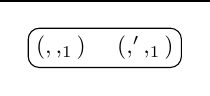
\begin{tikzpicture}[scale=0.85, every node/.style={transform shape}]

\node[rounded corners,draw](t0rx) {$(\otR, \key, \val_1)$ \quad $(\otW, \key', \val_1)$}; 

\end{tikzpicture}
\end{center}

It is important to note, however, that the set of abstract executions generated by $\prog$ 
is still bound to the structure of the program.
For example, executing $\prog$ under the anarchic execution model will never lead to 
an abstract execution with multiple transactions, 
or to an abstract execution where a transaction writes a key other than $\key'$ is written.

The \cref{def:axiom-to-cm} defines all the possible abstract executions 
induced by a axiomatic definition $(\RP, \Ax)$.

\begin{definition}[Programs under axiomatic definition]
\label{def:axiom-to-cm}
\label{def:axiom-to-prog}
The semantics of a program $\prog$ under a consistency model with axiomatic definition 
$(\RP, \Ax)$ is given by 
\[
\interpr{\prog}_{(\RP, \Ax)} = \Set{ \aexec }[ (\aexec_{0}, \thdenv_{0}, \prog) \toAEXEC{\_}_{(\RP, \Ax)}^{\ast} (\aexec, \stub, \prog_{f}) ]
\]
where $\thdenv_{0} = \lambda \cl \in \dom(\prog) \ldotp \lambda \vx \ldotp 0$ and $\prog_{f} = \lambda \cl \in \dom(\prog).\pskip$.
\end{definition}

We define the set of all the possible behaviours of a program $\prog$ to be $\interpr{\prog}_{\anarchic}$. 
One may argue that the axiomatic definition $\anarchicCM$ does not truly represent an anarchic consistency model. 
Consider the following code:
\[
\begin{session}
\begin{transaction}
\plookup{\pvar{a}}{\key}; \\
\plookup{\pvar{b}}{\key};\\
\pifs{\pvar{a} != \pvar{b}} \pmutate{\key'}{\val_1} \pife
\end{transaction}
\end{session}
\]
Under a even weaker anarchic consistency model, 
it would be possible for program $\prog'$ to write the value $\val_1$ for key $\key'$. 
However, this never happens if $\prog'$ is executed under our $\anarchicCM$.
Because we embedded into abstract execution the assumption that 
transactions only read at most one value for each key.

We can weaken the anarchic behaviours further by lifting this limitation 
and still retain the validity of all the results contained in this report.
However, the constraint that an object is never read twice in transactions is enforced by atomic visibility, 
so it is unnecessary to lift such limitation of our $\anarchicCM$.

The set of all possible behaviours exhibited by a program $\prog$ under a consistency model $(\RP, \Ax)$ 
can be defined by intersecting the set of executions that $\prog$ exhibits under the anarchic consistency model,
with the set of all executions allowed by the axiomatic definition $(\RP, \Ax)$ (\cref{thm:consistency-intersect-anarchic}).

\begin{theorem}
\label{thm:consistency-intersect-anarchic}
For any program $\prog$ and axiomatic definition $(\RP, \Ax)$:
\[
\interpr{\prog}_{(\RP, \Ax)} = \interpr{\prog}_{\anarchic} \cap \CMa(\RP, \Ax)
\]
\end{theorem}
\begin{proof}
    It is easy to see \( \interpr{\prog}_{(\RP, \Ax)} \subseteq \CMa(\RP, \Ax) \) by \cref{def:axiom-to-cm} 
    so \( \interpr{\prog}_{(\RP, \Ax)} \subseteq \interpr{\prog}_{\anarchic} \cap \CMa(\RP, \Ax) \).
    For another way, by \cref{prop:aexec-semantics-mono}, 
    we know \( \interpr{\prog}_{\anarchic} \subseteq \interpr{\prog}_{(\RP, \Ax)} \).
    Then, by the definition of \( \interpr{\prog}_{\stub} \), it follows
    \( \interpr{\prog}_{\anarchic} \cap \CMa(\RP, \Ax) \subseteq \interpr{\prog}_{(\RP, \Ax)} \).
\end{proof}


\begin{proposition}[Monotonic axiomatic definition]
\label{prop:aexec-semantics-mono}
Let define \( (\RP_1, \Ax_1) \sqsubseteq (\RP_2, \Ax_2) \) as the following:
\[
    \fora{\aexec,\txidset} \RP_2(\aexec,\txidset) \subseteq \RP_1(\aexec,\txidset)
\]
and,
\[
    \fora{\aexec} \bigcup_{\A_1 \in \Ax_1}\A_1(\aexec) \subseteq \bigcup_{\A_2 \in \Ax_2}\A_2(\aexec)
\]
then
\[ \interpr{\prog}_{(\RP, \Ax)} \subseteq \interpr{\prog}_{\anarchic} \]
\end{proposition}
\begin{proof}
    Since \( \anarchic \sqsubseteq (\RP, \Ax) \),
    We prove stronger result that for \( (\RP_1, \Ax_1) \sqsubseteq  (\RP_2, \Ax_2)\),
    the following  hold:
    \[
        \begin{array}{@{}l@{}}
            \fora{\cl, \aexec, \aexec', \prog, \prog', \stk, \stk'} 
            \cl \vdash ( \aexec, \stk ), \prog \toAEXEC{\stub}_{(\RP_1, \Ax_1)} ( \aexec', \stk' ), \prog' 
            \implies \cl \vdash ( \aexec, \stk ), \prog \toAEXEC{\stub}_{(\RP_2, \Ax_2)} ( \aexec', \stk' ), \prog' \\
        \end{array}
    \]
    We prove it by induction on the derivations.
    The only interesting case is the \rl{PAtomicTrans} rule.
    Given an initial runtime abstract execution \( \aexec \),
    a set of observable transactions \( \txidset \),
    a new transaction identifier \( \txid \),
    by the \rl{AAtomicTrans} rule, it is sufficient to prove, 
    first, all the snapshot under the stronger consistency model is also a valid snapshot under the weaker one:
    \begin{equation}
        \label{equ:obs-state-included}
        \fora{\aexec,\txidset} \RP_2(\aexec,\txidset) \subseteq  \RP_1(\aexec,\txidset)
    \end{equation}
    and second if it is valid  to commit a new transition with the observable set \( \txidset \) under stronger consistency model,
    it is able to do so under weaker consistency model:
    \begin{equation}
        \label{equ:consis-both-exist}
        \bigcup_{\A_1 \in \Ax_1}\A_1(\aexec')^{-1}(\txid) \subseteq \bigcup_{\A_2 \in \Ax_2}\A_2(\aexec')^{-1}(\txid)
    \end{equation}
    The \cref{equ:obs-state-included,equ:consis-both-exist} can be proven by \( (\RP_1, \Ax_1) \sqsubseteq  (\RP_2, \Ax_2) \).

    \caseB{\rl{PAssign}, \rl{PAssume}, \rl{PChoice}, \rl{PLoop}, \rl{PSeqSkipS}, \rl{PPar}, \rl{PWait}}
    These base cases do not depend on the consistency model, so they trivial hold because of the hypothesis.
    \caseI{\rl{PSeq}}
    It is proved directly by applying the \ih
\end{proof}


\section{Relationship between kv-stores and abstract execution}
\subsection{KV-Store to Abstract Executions}
\label{app:aexec2kv}
\label{sec:thm:aexec2kv-compatible-proof}

We introduce the definition of the dependency graph induced an abstract execution:

\begin{definition}
\label{def:aexec2graph}
Given an abstract execution $\aexec$ that satisfies the last write wins policy,
the dependency graph $\graphOf[\aexec] \defeq (\TtoOp{T}_{\aexec}, \WR_{\aexec}, 
\WW_{\aexec}, \RW_{\aexec})$ is defined by letting
\begin{itemize}
\item $\txid \toEDGE{\WR_{\aexec}(\key)} \txid'$ if and only if 
$\txid = \max_{\AR_{\aexec}}(\visibleWrites_{\aexec}(\key, \txid'))$, 
\item $\txid \toEDGE{\WW_{\aexec}(\key)} \txid'$ if and only 
$\txid, \txid' \in_{\aexec} (\otW, \;\key, \stub)$ 
and $\txid \toEDGE{\AR_{\aexec}} \txid'$,
\item $\txid \toEDGE{\RW_{\aexec}(\key)} \txid'$ if and only if either 
$(\otR, \key, \stub) \in_{\aexec} \txid, (\otW, \key, \stub) \in_{\aexec} \txid'$ and 
whenever $\txid'' \toEDGE{\WR_{\aexec}(\key)} \txid$, 
then $\txid'' \toEDGE{\WW_{\aexec}(\key)} \txid'$.
\end{itemize}
\end{definition}

Note that each abstract execution $\aexec$ determines a kv-store $\mkvs_{\aexec}$,
as a result of \cref{def:aexec2graph} and \cref{thm:kv2graph}. 
Let $\mkvs$ be the unique kv-store such that $\Gr_{\mkvs} = \graphOf[\aexec]$, then $\mkvs_{\aexec} = \mkvs$. 
As we will discuss later in this Section,
this mapping $\mkvs_{(\stub)}$ is NOT a bijection, 
in that several abstract executions may be encoded in the same kv-store.
Because kv-stores abstract away the total arbitration order of transactions.

Upon the relation \( \mkvs_{\aexec} = \mkvs \),
there is a deeper link between kv-store plus views and abstract exertions.
This notion, named \emph{compatibility}, bases on the intuition that 
clients can make observations over kv-stores and abstract executions, in terms of snapshots.

In kv-stores, observations are snapshots induced by views. 
While in abstract executions, observations correspond to the snapshots induced by the visible transactions.
Note that it is under the condition that the abstract execution adopts $\RP_{\LWW}$ resolution policy.
This approach is analogous to the one used by operation contexts in \cite{repldatatypes}.
Thus, a kv-store $\mkvs$ is \emph{compatible} with an abstract execution $\aexec$, written \( \mkvs \compatible \aexec \)
if any observation made on $\mkvs$ can be replicated by an observation made on $\aexec$, and vice-versa. 

\begin{definition}
\label{def:compatible}
Given a kv-store $\mkvs$,
an abstract execution $\aexec$ is compatible with $\mkvs$, written 
$\aexec \compatible \mkvs$, if and only if there exists a  mapping 
$f: \pset{\txidset_{\aexec}} \rightarrow \Views(\mkvs)$
such that  
\begin{itemize}
\item for any subset $\txidset \subseteq \txidset_{\aexec}$, then $\RP_{\LWW}(\aexec, \txidset) = \Set{\snapshot[\mkvs, f(\txidset)]}$; 
\item for any view $\vi \in \Views(\mkvs)$, there exists a subset $\txidset \subseteq \txidset_{\aexec}$ 
such that $f(\txidset) = \vi$, and $\RP_{\LWW}(\aexec, \txidset) = \Set{\snapshot[\mkvs_{\aexec}, \vi]}$.
\end{itemize}
\end{definition}

The function $\getView[\aexec, \txidset]$ defines the view on \( \mkvs_\aexec \) that corresponds to \( \txidset \) as the following:
\[
    \getView[\aexec, \txidset] \defeq \lambda \key. \Set{0} \cup \Set{i}[\wtOf(\mkvs_{\aexec}(\key, i)) \in \txidset]
\]
Inversely, the function \( \Tx[\mkvs, \vi] \) converts a view to a set of observable transactions:
\[
    \Tx[\mkvs, \vi] \defeq \Set{\wtOf(\mkvs(\key, i))}[\key \in \Keys \land i \in \vi(\key)]
\]
Given \( \getView \), \( \Tx \), \cref{def:compatible}, 
it follows \( \aexec \compatible \mkvs_{\aexec} \) shown in \cref{thm:aexec2kv.compatible}.

\begin{theorem}
\label{thm:aexec2kv.compatible}
For any abstract execution $\aexec$ that satisfies the last write wins policy, $\aexec \compatible \mkvs_{\aexec}$.
\end{theorem}
\begin{proof}
Given the function $\getView[\aexec, \cdot]$ from $\pset{\txidset_{\aexec}}$ to $\Views(\mkvs_{\aexec})$,
we prove it satisfies the constraint of \cref{def:compatible}.
Fix a set of transitions \( \txidset \).
By the \cref{prop:getview.valid}, the view $\getView[\aexec, \txidset]$  on \( \mkvs_\aexec \) is a valid view,
that is, \( \getView[\aexec, \txidset] \in \Views(\mkvs_\aexec) \).
Given that it is a valid view, the \cref{prop:compatible.aexec2kv} proves:
\begin{equation}
    \label{equ:visible-trans-to-view}
    \RP_{\LWW}(\aexec, \txidset) = \Set{\snapshot[\mkvs_{\aexec}, \getView[\aexec, \txidset]]} 
\end{equation}

The another way round is more subtle,
because \( \txidset \) contains any read only transaction.
By \cref{prop:getview.tx}, it is safe to erase read only transactions from \( \txidset \),
when calculating the view \( \getView[\aexec, \txidset] \).
Last, by \cref{prop:compatible.kv2aexec}, we prove the following:
\begin{equation}
    \label{equ:view-to-visible-trans}
    \RP_{\LWW}(\aexec, \txidset) = \snapshot[\mkvs_{\aexec}, \vi]
\end{equation}
By \cref{equ:visible-trans-to-view} and \cref{equ:view-to-visible-trans},
it follows \( \aexec \compatible \mkvs_{\aexec} \).
\end{proof}

\begin{proposition}[Valid views]
\label{prop:getview.valid}
For any abstract execution $\aexec$, and $\txidset \subseteq \txidset_{\aexec}$, 
$\getView[\aexec, \txidset] \in \Views(\mkvs_{\aexec})$.
\end{proposition}
\begin{proof}
Assume an abstract execution $\aexec$, a set of transactions $\txidset \subseteq \txidset_{\aexec}$, and a key \( \key \).
By the definition of $\getView[\aexec, \txidset]$, 
then $0 \in \getView[\aexec, \txidset](\key)$, and 
$0 \leq i < \abs{ \mkvs_{\aexec}(\key) }$ for any index \( i \) such that $i \in \getView[\aexec, \txidset](\key)$.
Therefore we only need to prove that $\getView[\aexec, \txidset]$ satisfies \eqref{eq:view.atomic}.
Let $j \in \getView[\aexec, \txidset](\key)$ for some key $\key$, and let $\txid = 
\wtOf(\mkvs_{\aexec}(\key, j))$. Let also $\key', i$ be such that 
$\wtOf(\mkvs_{\aexec}(\key', i)) = \txid$. We need to show that 
$i \in \getView[\aexec, \txidset](\key')$. Note that it $\txid = \txid_{0}$ 
then $\wtOf(\mkvs_{\aexec}(\key', i)) = \txid$ only if $i = 0$, and 
$0 \in \getView[\aexec, \txidset](\key')$ by definition. 
Let then $\txid \neq \txid_{0}$. Because $\wtOf(\mkvs_{\aexec}(\key, j)) = \txid$ 
and $j \in \getView[\aexec, \txidset]$, then it must be the case that $\txid \in \txidset$. 
Also, because $\wtOf(\mkvs_{\aexec}(\key', i)) = \txid$, then $(\otW, \key, \stub) \in 
\TtoOp{T}_{\aexec}(\txid)$. It follows that there exists an index $i' \in \getView[\aexec, \txid](\key')$ 
such that $\wtOf(\mkvs_{\aexec}(\key', i')) = \txid$. By definition of 
$\mkvs_{\aexec}$, if $\wtOf(\mkvs_{\aexec}(\key', i')) = \txid$, then it must 
be $i' = i$, and therefore $i \in \getView[\aexec, \txid](\key')$.
\end{proof}


\begin{proposition}[Visible transactions to views]
\label{prop:compatible.aexec2kv}
For any subset $\txidset \subseteq \txidset_{\aexec}$, $\RP_{\LWW}(\aexec, \txidset) = \Set{\snapshot[\mkvs_{\aexec}, \getView[\aexec, \txidset]]}$.
\end{proposition}

\begin{proof}
Fix $\txidset \subseteq \aexec$, and let $\Set{\mkvs} = \RP_{\LWW}(\aexec, \txidset)$. We prove that, for any $\key \in \Keys$, 
$\mkvs(\key) = \snapshot[\getView[\aexec, \txidset]](\key)$. There are two different cases: 
\begin{enumerate}
    \item $\txidset \cap \Set{ \txid }[ (\otW, \key, \stub) \in_{\aexec} \txid ] = \emptyset$. 
In this case $\mkvs(\key) = \val_0$. 
We know that $\graphOf[\aexec]$ satisfies all the constraints required by the definition of dependency graph 
(\cite{laws}). Together with \cref{thm:kv2graph} it follows that $\mkvs_{\aexec}(\key, 0) = (\val_0, \txid_0, \stub)$.
We prove that $\getView[\aexec, \txidset](\key) = \Set{0}$, 
hence 
\[ 
\snapshot[\mkvs_{\aexec}, \getView[\aexec, \txidset]](\key) = \valueOf(\mkvs_{\aexec}(\key, 0)) = \val_{0}
\]
Note that whenever $(\otW, \key, \stub) \in_{\aexec} \txid$ for some $\txid$, then 
$\txid \notin \txidset$. Therefore, whenever $(\val, \txid, \stub) = \mkvs_{\aexec}(\key, i)$ for some $i \geq 0$, then 
$\txid \notin \txidset$.
\[
\getView[\aexec, \txidset](\key) = \Set{0} \cup \Set{i }[ \wtOf(\mkvs_{\aexec}(\key, i)) \in \txidset)] = \Set{0} \cup \emptyset = \Set{0}
\]
\item Suppose now that $\txidset \cap \Set{ \txid }[ (\otW, \key, \stub) \in_{\aexec} \txid ] \neq \emptyset$. 
Let then $\txid = \max_{\AR_{\aexec}}(\txidset \cap \Set{\txid }[ (\otW, \key, \stub) \in_{\aexec} \txid])$. 
Then $(\otW, \key, \val) \in_{\aexec} \txid$ for some $\val \in \Val$. Furthermore, $\RP_{\LWW}(\aexec, \txidset)(\key) = \val$.
By definition, $\txid' \in \txidset \cap \Set{ \txid }[ (\otW, \key, \stub) \in_{\aexec} \txid]$, 
then either $\txid' = \txid$ or $\txid' \toEDGE{\AR_{\aexec}} \txid$. The definition of 
$\graphOf[\aexec]$ gives that $\txid' \toEDGE{\WW_{\aexec}(\key)} \txid$. 
Because $(\otW, \key, \val) \in_{\aexec} \txid$, then there exists an index 
$i \geq 0$ such that $\mkvs_{\aexec}(\key, i) = (\val, \txid, \stub)$. Furthermore, 
whenever $\wtOf(\key, j) = \txid'$ for some $\txid'$ and $j > i$, then it must 
be the case that $\txid \toEDGE{\WW_{\aexec}(\key)} \txid'$, and because 
$\WW_{\aexec}(\key)$ is transitive and irreflexive, it must be that  
$\neg( \txid' \toEDGE{\WW_{\aexec}(\key)} \txid)$ and $\txid \neq \txid'$: this implies that 
$\txid' \notin \txidset$. It follows that $\max(\getView[\aexec, \txidset](\key)) = i$, hence 
$\snapshot[\mkvs_{\aexec}, \getView[\aexec, \txidset]] = \valueOf(\mkvs_{\aexec}(\key, i)) = \val$.
\end{enumerate}
\end{proof}

\begin{proposition}[Read-only transactions erasing]
\label{prop:getview.tx}
Let $\vi \in \Views(\mkvs_{\aexec})$, and let $\txidset \subseteq \txidset_{\aexec}$ be a 
set of read-only transactions in $\aexec$. Then 
$\getView[\aexec, \txidset \cup \Tx[\mkvs_{\aexec}, \vi]] = \vi$. 
\end{proposition}

\begin{proof}
Fix a key $\key$. Suppose that $i \in \getView[\aexec, \txidset \cup \Tx[\mkvs_{\aexec}, \vi]](\key)$. 
By definition, $\mkvs_{\aexec}(\key, j) = (\stub, \txid, \stub)$ for some $\txid \in \txidset \cup \Tx[\mkvs_{\aexec}, \vi]$. 
Because $\txidset$ only contains read-only transactions, by definition of $\mkvs_{\aexec}$ there exists 
no index $j$ such that $\mkvs_{\aexec}(\key, j) = (\stub, \txid', \stub)$ for some $\txid' \in \txidset$, 
hence it must be the case that $\txid \in \Tx[\mkvs_{\aexec}, \vi]$. By definition of $\Tx$, 
this is possible only if there exist a key $\key'$ and an index $j$ such that $\mkvs_{\aexec}(\key', \vi) = (\stub, \txid, \stub)$. 
Because $\vi$ is atomic by definition, and because $\mkvs_{\aexec}(\key, i) = (\stub, \txid, \stub)$, then we have that $i \in \vi(\key)$. 

Now suppose that $i \in \vi(\key)$, and let $\mkvs_{\aexec}(\key, i) = (\stub, \txid, \stub)$ for some $\txid$. 
This implies that $(\otW, \key, \stub) \in_{\aexec} \txid$.
By definition $\txid \in \Tx[\mkvs_{\aexec}, \vi]$, hence $\txid \in \txidset \cup \Tx[\mkvs_{\aexec}, \vi)]$. 
Because $\txid \in \txidset \cup \Tx[\mkvs_{\aexec}, \vi]$, then for any key $\key'$ such that 
$(\otW, \key', \stub) \in_{\aexec} \txid$, there exists an index $j \in \getView[\aexec, \txidset \cup \Tx[\mkvs_{\aexec}, \vi]]$ 
$\mkvs(\key', j) = (\stub, \txid, \stub)$; because kv-stores only allow a transaction to write at most one version 
per key, then the index $j$ is uniquely determined. In particular, we know that $(\otW, \key, \stub) \in_{\aexec} \txid$, 
and $\mkvs_{\aexec}(\key, i) = (\stub, \txid, \stub)$, from which it follows that $i \in \getView[\aexec, \txidset \cup \Tx[\mkvs_{\aexec}, \vi]](\key)$.
\end{proof}


\begin{proposition}[Views to visible transactions]
\label{prop:compatible.kv2aexec}
Given a view $\vi \in \Views(\mkvs_{\aexec})$, there exists $\txidset \subseteq \txidset_{\aexec}$ 
such that $\getView[\aexec, \txidset] = \vi$, and $\RP_{\LWW}(\aexec, \txidset) = \snapshot[\mkvs_{\aexec}, \vi]$.
\end{proposition}

\begin{proof}
We only need to prove that, for any $\vi \in \Views(\mkvs_{\aexec})$, there exists $\txidset \subseteq \txidset_{\aexec}$ such 
that $\getView[\aexec, \txidset] = \vi$. Then it follows from \cref{prop:compatible.aexec2kv} that 
$\RP_{\LWW}(\aexec, \txidset) = \snapshot[\mkvs_{\aexec}, \vi]$. 
It suffices to choose $\txidset = \bigcup_{\key \in \Keys}(\Set{\wtOf(\mkvs_{\aexec}(\key, i))}[ i > 0 \land i \in \vi(\key)])$.
Fix a key $\key$, and let $i \in \vi(\key)$. We prove that $i \in \getView[\aexec, \txidset]$. 
If $i = 0$, then $i \in \getView[\aexec, \txidset]$ by definition. 
Therefore, assume that $i > 0$. Let $\txid = \wtOf(\mkvs_{\aexec}(\key, i))$.
It must be the case that $\txid \in \txidset$ and $i \in \getView[\aexec, \txidset](\key)$.

Next, suppose that $i \in \getView[\aexec, \txidset](\key)$. We prove that $i \in \vi(\key)$.
Note that if $i = 0$, then $i \in \vi(\key)$ because of the 
definition of views. Let then $i > 0$. Because $i \in \getView[\aexec, \txidset](\key)$, we have that 
$\wtOf(\mkvs_{\aexec}(\key, i)) \in \txidset$.  Let $\txid = \wtOf(\mkvs_{\aexec}(\key, i))$. Because $i > 0$, 
it must be the case that $\txid \neq \txid_0$.
By definition, $\txid \in \txidset$ only if there 
exists an index $j$ and key $\key'$, possibly different from $\key$, such that $\wtOf(\mkvs_{\aexec}(\key', j)) = \txid$ and $j \in \vi(\key')$. 
Because $\txid \neq \txid_0$ we have that $j > 0$. Finally, because $\vi$ is atomic by definition, $j \in \vi(\key')$
$\wtOf(\mkvs_{\aexec}(\key', j)) = \txid = \wtOf(\mkvs_{\aexec}(\key, i))$, then it must be the case 
that $i \in \vi(\key)$, which concludes the proof.
\end{proof}


\subsection{KV-Store Traces to Abstract Execution Traces}
\label{sec:kvtrace2aexec}

To prove our definitions using execution test on kv-stores 
is sound and complete with respect with the axiomatic definitions on abstract executions (\cref{sec:kv-sound-complete-proof}),
we need to prove trace equivalent between these two models.

In this section, we only consider the trace that does not involve \( \prog \) but only committing fingerprint and view shift.
In \cref{sec:et-sound-complete-constructor}, we will go further and discuss the trace installed with \( \prog \).

Similar to \(\anarchic\), let $\ET_\top$ be the most permissive execution test.
That is $\ET_\top \vdash (\mkvs, \vi) \csat \fp: (\mkvs',\vi')$ 
such that whenever $\vi(\key) \neq \vi'(\key)$ then either $(\otW, \key, \stub) \in \fp$ or $(\otR, \key, \stub) \in \fp$.
%{\color{red} I forgot this last constraint in the latest version of the document, definitions 
%and proofs of theorems that follow must be re-factored to take the constraint into account.}
We will relate $\ET_{\top}$-traces to abstract executions that satisfy the last write wins resolution policy, \ie \( (\RP_{\LWW}, \emptyset) \).

To bridge $\ET_{\top}$-traces to abstract executions, 
The \aeset(\tr) function converse the trace of \( \ET_\top \) to set of possible abstract executions (\cref{def:kvtrace2aexec}).
In fact, for any trace \( \tr \) and abstract execution $\aexec \in \aeset(\tr)$, 
the last configuration of $\tr$ is $(\mkvs_{\aexec}, \stub)$ (\cref{prop:kvtrace2aexec}).
We often use \( \aexec_\tr \) for \( \aexec \in \aeset(\tr) \).

\begin{definition}
\label{def:kvtrace2aexec}
Given a kv-store $\mkvs$, a view $\vi$, 
an initial abstract execution $\aexec_0 = ( [ ], \emptyset, \emptyset)$, 
an abstract execution $\aexec$, a set of transactions  
$\txidset \subseteq \txidset_{\aexec}$, a transaction identifier $\txid$ and a set of operations $\fp$,
the \( \extend \)  function defined as the follows:
\begin{align*}
\extend[\aexec, \txid, \txidset, \fp] & \defeq 
\begin{cases}
\text{undefined} & \text{if} \ \txid = \txid_{0}\\
\left(\TtoOp{T}_{\aexec} \uplus \Set{\txid \mapsto \fp}, \VIS', \AR' \right) & \text{if} \ \dagger \\
\end{cases} \\
\dagger & \equiv 
\begin{multlined}[t]
\txid = \txid_{\cl}^{n}
\land \VIS' = \VIS_{\aexec} \uplus \Set{(\txid', \txid)}[\txid \in \txidset]  \\
{} \land \AR' = \AR_{\aexec} \uplus \Set{(\txid', \txid)}[\txid' \in \txidset_{\aexec}]
\end{multlined}
\end{align*}
Given a $\ET_{\top}$ trace $\tr$, let $\lastConf(\tr)$ be the last configuration appearing in $\tr$.
The set of abstract executions $\aeset(\tr)$ is defined as the smallest set such that:
\begin{itemize}
\item $\aexec_{0} \in \aeset((\mkvs_{0}, \vienv_{0}))$, 
\item if $\aexec \in \aeset(\tr)$, then $\aexec \in \aeset\left(\tr \toET{(\cl, \varepsilon)}[\ET_{\top}] (\mkvs, \vienv) \right)$, 
\item if $\aexec \in \aeset(\tr)$, then $\aexec \in \aeset\left(\tr \toET{(\cl, \emptyset)}[\ET_{\top}] (\mkvs, \vienv) \right)$, 
\item 
    let $(\mkvs', \vienv') = \lastConf(\tr)$; 
    if $\aexec \in \aeset(\tr)$, $\fp \neq \emptyset$,
    and $\txidset = \Tx[\mkvs, \vienv'(\cl)] \cup \txidset_\rd$ where \( \txidset_\rd \) is a set of \emph{read-only transactions}
    such that $(\otW, \key, \val) \notin_{\aexec} \txid'$ for all keys \( \key \) and values \( \val \) and transactions \( \txid' \in \txidset_\rd\),
    and if the transaction $\txid$ is the transaction appearing in $\lastConf(\tr)$ but not in $\mkvs$, 
    then $\extend(\aexec, \txid, \txidset, \fp) \in \aeset\left(\tr \toET{(\cl, \fp)}[\ET_{\top}] (\mkvs, \vienv) \right)$.
\end{itemize}
\end{definition}

\begin{proposition}[Trace of \( \ET \) to abstract executions]
\label{prop:kvtrace2aexec}
For any $\ET_{\top}$-trace $\tr$, 
the abstract execution $\aexec \in \aeset(\tr)$ satisfies the last write wins policy,
and $(\mkvs_{\aexec}, \stub) = \lastConf(\tr)$.
\end{proposition}
\begin{proof}
Fix a $\ET_{\top}$-trace $\tau$. 
We prove by induction on the number of transitions $n$ in $\tau$. 
\begin{itemize}
\item \caseB{$n = 0$}
It means $\tr = (\mkvs_{0}, \stub)$.
It follows from \cref{def:kvtrace2aexec} that $\aexec_{\tau} = ([], \emptyset, \emptyset)$. 
This triple satisfies the constraints of \cref{def:aexec}, as well as the resolution policy $\RP_{\LWW}$. 
It is also immediate to see that $\graphOf(\aexec) = ([], \emptyset, \emptyset, \emptyset)$.
In particular, $\txidset_{\graphOf(\aexec)} = \emptyset$, 
and the only kv-store $\mkvs$ such that $\txidset_{\Gr_{\mkvs}} = \emptyset$ 
is given by $\mkvs = \mkvs_{0}$. 
By definition, $\mkvs_{\aexec_{\tr}} = \mkvs_{0}$, as we wanted to prove.

\item \caseI{$n > 0$} In this case, we have that $\tr = \tr' \toET{(\cl, \mu)} (\mkvs, \vienv)$ 
for some $\cl, \mu, \mkvs, \vienv$. The $\ET_{\top}$-trace $\tau'$ contains exactly $n-1$ transitions, 
so that by induction we can assume that $\aexec_{\tau'}$ is a valid abstract execution that satisfies 
$\RP_{\LWW}$. and $\lastConf(\tau') = (\mkvs_{\aexec_{\tau'}}, \vienv')$ for some $\vienv'$. 

We perform a case analysis on $\mu$. 
If $\mu = \varepsilon$, then it follows that $\mkvs = \mkvs_{\aexec_{\tau'}}$, 
and $\aexec_{\tau} = \aexec_{\tau'}$ by \cref{def:kvtrace2aexec}. 
Then by the inductive hypothesis $\aexec_{\tau}$ is an abstract execution that satisfies $\RP_{\LWW}$,
$\lastConf(\tau) = (\mkvs, \stub)$, and $\mkvs_{\aexec_{\tau}} = \mkvs_{\aexec_{\tau'}} = \mkvs$, 
and there is nothing left to prove. 

Suppose now that $\mu = \fp$, for some $\fp$. In this case we have that  
$\mkvs \in \updateKV[\mkvs_{\aexec_{\tau'}}, \vienv'(\cl), \fp, \cl]$. Note that if 
$\fp = \emptyset$, then $\mkvs = \mkvs_{\aexec_{\tau'}}$ and $\aexec_{\tau} = \aexec_{\tau'}$. 
By the inductive hypothesis, $\aexec_{\tau}$ is an abstract execution that satisfies 
$\RP_{\LWW}$, and $\mkvs = \mkvs_{\aexec_{\tau'}} = \mkvs_{\aexec_{\tau}}$. 
Assume then that $\fp \neq \emptyset$. 
By definition, $\mkvs = \updateKV[\mkvs_{\aexec_{\tau'}}, \vienv'(\cl), \fp, \txid]$ 
for some $\txid \in \nextTxid(\cl, \mkvs_{\aexec_{\tau}})$. It follows that $\txid$ 
is the unique transaction such that $\txid \notin \mkvs_{\aexec_{\tau'}}$, and $\txid \in \mkvs$ 
(the fact that $\txid \in \mkvs$ follows from the assumption that $\fp \neq \emptyset$). Let 
$\txidset = \Tx[\mkvs_{\aexec_{\tau'}}, \vienv'(\cl)]$; then $\aexec_{\tau} = \extend(\mkvs_{\aexec_{\tau'}}, \txid, \txidset, \fp)$. 
Note that $\aexec_{\tau}$ satisfies the constraints of abstract execution required by \cref{def:aexec}:
\begin{itemize}
\item  Because $\txid \in \nextTxid(\cl, \mkvs_{\aexec_{\tau}})$, it must be the case that $\txid = \txid_{\cl}^{m}$ for some 
$m \geq 1$; we have that $\TtoOp{T}_{\aexec_{\tau}} = \TtoOp{T}_{\aexec_{\tau'}}\rmto{\txid_{\cl}^{m}}{\fp}$, 
from which it follows that 
\[
\txidset_{\aexec_{\tau}} = \dom(\TtoOp{T}_{\aexec_{\tau}}) = \dom(\TtoOp{T}_{\aexec_{\tau'}}) \cup 
\Set{\txid_{\cl}^{m} } = \txidset_{\aexec_{\tau'}} \cup \Set{\txid_{\cl}^{m} }
\]
By inductive hypothesis, $\txid_0 \notin \txidset_{\aexec_{\tau'}}$, and therefore $\txid_{0} \notin 
\txidset_{\aexec_{\tau'}} \cup \Set{\txid_{\cl}^{m} } = \txidset_{\aexec}$.

\item \( \VIS_{\aexec_{\tau}} \subseteq \AR_{\aexec_{\tau}} \).
    Let $(\txid' ,\txid'') \in \VIS_{\aexec_{\tau}}$. Then either $\txid'' = \txid_{\cl}^{m}$ and $\txid' \in \txidset$, or $(\txid', \txid'') \in 
\VIS_{\aexec_{\tau'}}$. In the former case, we have that $(\txid', \txid_{\cl}^{m}) \in \AR_{\aexec_{\tau}}$ by definition; 
in the latter case, we have that $(\txid', \txid'') \in \AR_{\aexec_{\tau'}}$ because $\aexec_{\tau'}$ is a valid 
abstract execution by inductive hypothesis, and therefore $(\txid', \txid'') \in \AR_{\aexec_{\tau}}$ by definition. 
This concludes the proof that $\VIS_{\aexec_{\tau}} \subseteq \AR_{\aexec_{\tau}}$. 
\item \( \VIS_{\aexec_\tr} \) is irreflexive.
Assume $(\txid', \txid'') \in \VIS_{\aexec_{\tau}}$, then either 
$(\txid' \txid'') \in \VIS_{\aexec_{\tau'}}$, and because $\VIS_{\aexec_{\tau'}}$ is irreflexive by the inductive hypothesis, 
then $\txid' \neq \txid''$; 
or $\txid'' = \txid_{\cl}^{m}$, $\txid' \in \txidset \subseteq \txidset_{\aexec_{\tau'}}$, 
and because $\txid_{\cl}^{m} \notin \mkvs_{\aexec_{\tau'}}$, then $\txid' \neq \txid_{\cl}^{m}$. 

\item $\AR_{\aexec_{\tau}}$ is total. Let $(\txid', \txid'') \in \txidset_{\aexec_{\tau}}$. 
Suppose that $\txid' \neq \txid''$.
\begin{enumerate}
\item If $\txid' \neq 
\txid_{\cl}^{m}$, $\txid'' \neq \txid_{\cl}^{m}$, then it must be the case that $\txid', \txid'' \in \txidset_{\aexec_{\tau'}}$; 
this is because we have already argued that $\txidset_{\aexec_{\tau}} = \txidset_{\aexec_{\tau'}} \cup \Set{\txid_{\cl}^{m}}$. 
By the inductive hypothesis, we have that either $(\txid', \txid'') \in \AR_{\aexec_{\tau'}}$, or 
$(\txid'', \txid') \in \AR_{\aexec_{\tau'}}$. Because $\AR_{\aexec_{\tau'}} \subseteq \AR_{\aexec_{\tau}}$, 
then either $(\txid', \txid'') \in \AR_{\aexec_{\tau'}}$ or $(\txid'', \txid') \in \AR_{\aexec_{\tau}}$. 
\item if $\txid'' = \txid_{\cl}^{m}$, then it must be $\txid' \in \txidset_{\aexec_{\tau'}}$. By definition, 
$(\txid', \txid_{\cl}^{m}) \in \AR_{\aexec_{\tau}}$. Similarly, if $\txid' = \txid_{\cl}^{m}$, we 
can prove that $(\txid'', \txid_{\cl}^{m}) \in \AR_{\aexec_{\tau}}$.
\end{enumerate}
\item  $\AR_{\aexec_{\tau}}$ is irreflexive. It follows is the same as the one of $\VIS_{\aexec_{\tau}}$.
\item \( \AR_{\aexec_{\tau}} \) is transitive.
Assume $(\txid', \txid'') \in \AR_{\aexec_{\tau}}$ and $(\txid'', \txid''') \in \AR_{\aexec_{\tau}}$. 
Note that it must be the case that $\txid', \txid'' \in \txidset_{\aexec_{\tau'}}$ by the definition of 
$\AR_{\aexec}$, and in particular $(\txid', \txid'') \in \AR_{\aexec_{\tau'}}$. 
For $\txid'''$, we have two possible cases. 
\begin{enumerate}
\item Either $\txid''' \in \txidset_{\aexec_{\tau}}$, from 
which it follows that $(\txid'', \txid''') \in \AR_{\aexec_{\tau'}}$; because
of $\AR_{\aexec_{\tau'}}$ is transitive by the inductive hypothesis, then 
$(\txid', \txid''') \in \AR_{\aexec_{\tau'}}$, and therefore $(\txid' ,\txid''') \in 
\AR_{\aexec_{\tau}}$.
\item Or $\txid''' = \txid_{\cl}^{m}$, and because $\txid' \in \txidset_{\aexec_{\tau'}}$, then 
$(\txid', \txid_{\cl}^{m}) \in \AR_{\aexec_{\tau}}$ by definition. 
\end{enumerate}
\item \( \SO_{\aexec_{\tau}} \subseteq \AR_{\aexec_{\tau}} \).
Let $\cl'$ be a client such that $(\txid_{\cl'}^{i}, \txid_{\cl'}^{j}) \in \AR_{\aexec_{\tau}}$. 
If $\cl' \neq \cl$, then it must be the case that $\txid_{\cl'}^{i}, \txid_{\cl'}^{j} \in \txidset_{\aexec_{\tau'}}$, 
and therefore $(\txid_{\cl'}^{i}, \txid_{\cl'}^{j}) \in \AR_{\aexec_{\tau'}}$. By the inductive hypothesis, 
it follows that $i < j$. If $\cl' = \cl$, then by definition of $\AR_{\aexec_{\tau}}$ it must be  $i \neq m$. 
If $j \neq m$ we can proceed as in the previous case to prove that $i < j$. If $j = m$, then 
note that $\txid_{\cl}^{i} \in \txidset_{\aexec_{\tau}}$ only if $\txid_{\cl}^{i} \in \mkvs_{\aexec_{\tau'}}$. 
Because $\txid_{\cl}^{m} \in \nextTxid(\mkvs_{\aexec_{\tau'}}, \cl)$, then we have that $i < m$, 
as we wanted to prove.
\end{itemize}

Next, we prove that $\aexec_{\tau}$ satisfies the last write wins policy. 
Let $\txid' \in \txidset_{\aexec_{\tau}}$, and suppose that $(\otR, \key, \val) \in_{\aexec_{\tau}} \txid'$. 
\begin{itemize} 
\item If $\txid' \neq \txid$, then we have that $\txid \in \txidset_{\aexec_{\tau'}}$. We also have that 
$\VIS^{-1}_{\aexec_{\tau}}(\txid') = \VIS^{-1}_{\aexec_{\tau'}}(\txid')$, $\AR^{-1}_{\aexec_{\tau}}(\txid') 
= \AR^{-1}_{\aexec_{\tau'}}(\txid')$; finally, for any $\txid'' \in \txidset_{\aexec_{\tau'}}$, 
$(\otW, \key, \val') \in_{\aexec_{\tau}} \txid''$ if and only if $(\otW, \key, \val') \in_{\aexec_{\tau'}} 
\txid''$. Therefore, let $\txid_{r} = \max_{\AR_{\aexec_{\tau}}}(\VIS^{-1}_{\aexec_{\tau}}(\txid') \cap 
\Set{\txid'' }[ (\otW, \key, \stub) \in_{\aexec_{\tau}} \txid''])$. We have that $\txid_{r} = \max_{\AR_{\aexec_{\tau'}}}(\VIS^{-1}_{\aexec_{\tau'}}(\txid) 
\cap \Set{ \txid'' }[ (\otW, \key, \stub \in_{\aexec_{\tau'}} \txid''])$, and because $\aexec_{\tau'}$ satisfies the last write 
wins resolution policy,then $(\otW, \key, \val) \in_{\aexec_{\tau'}} \txid_{r}$. This also implies that 
$(\otW, \key, \val) \in_{\aexec_{\tau}} \txid_{r}$. 

\item Now, suppose that $\txid' = \txid$. Suppose that $(\otR, \key, \val) \in_{\aexec_{\tau}} \txid'$. 
By definition, we have that $(\otR, \key, \val) \in \fp$. Recall that $\tau = \tau' \toET{(\cl, \fp)}[\ET_{\top}] (\mkvs, \vienv)$, 
and $\lastConf(\tau') = (\mkvs_{\aexec_{\tau'}}, \vienv')$ for some $\vienv'$. 
That is, 
\[
    (\mkvs_{\aexec_{\tau'}}, \vienv') \toET{(\cl, \fp)}[\ET_{\top}] (\mkvs, \vienv)
\]
which in turn implies that $\ET_{\top} \vdash (\mkvs_{\aexec_{\tau'}}, \vienv'(\cl)) \csat \fp : (\mkvs,\vienv(\cl) )$. 
Let then $r = \max\Set{i}[ i \in \vienv'(\cl)(\key)]$. 
By definition of execution test, and because $(\otR, \key, \val) \in \fp$, then it must be the case that 
$\mkvs_{\aexec_{\tau'}}(\key, r) = (\val, \txid'', \stub)$ for some $\txid''$. 

We now prove that 
$\txid'' = \max_{\AR_{\aexec_{\tau}}}(\VIS^{-1}_{\aexec_{\tau}}(\txid) \cap \Set{ \txid'' }[ (\otW, \key, \stub) \in_{\aexec_{\tau}} \txid''])$. 
First we have
\[ 
\begin{array}{l}
\VIS^{-1}_{\aexec_{\tau}}(\txid) = 
\Tx[\mkvs_{\aexec_{\tau'}}, \vienv'(\cl)] = 
\Set{\wtOf(\mkvs_{\aexec_{\tau'}}(\key',  i)) }[ \key' \in \Keys \land  i \in \vienv'(\cl)(\key')]
\end{array}
\]
Note that $r \in \vienv'(\cl)(\key)$, and $\txid'' = \wtOf(\mkvs_{\aexec_{\tau'}}(\key, r))$. 
Therefore, $\txid'' \in \VIS^{-1}_{\aexec_{\tau}}(\txid)$. 
Because $\mkvs = \updateKV[\mkvs_{\aexec_{\tau'}}, \vienv'(\cl), \fp, \txid]$, it 
must be the case that $\wtOf(\mkvs(\key, r)) = \txid''$. Also, because $\wtOf(\mkvs_{\aexec_{\tau'}}(\key, r)) = \txid''$, 
then $(\otW, \key, \stub) \in_{\aexec_{\tau''}} \txid''$, or equivalently $(\otW, \key, \stub) \in \TtoOp{T}_{\aexec_{\tau'}}(\txid'')$. 
We have already proved that $\VIS_{\aexec_{\tau}}$ is irreflexive, hence it must be the case that $\txid'' \neq \txid$. 
In particular, because $\aexec_{\tau} = \extend(\aexec_{\tau'}, \txid, \stub, \stub)$, then we have that 
$\TtoOp{T}_{\aexec_{\tau}}(\txid'') = \TtoOp{T}_{\aexec_{\tau'}}\rmto{\txid}{\fp}(\txid'') = 
\TtoOp{T}_{\aexec_{\tau'}}(\txid'')$, hence $(\otW, \key, \stub) \in \TtoOp{T}_{\aexec_{\tau}}(\txid'')$. Equivalently, 
$(\otW, \key, \stub) \in_{\aexec_{\tau}} \txid''$. We have proved that $\txid'' \in \VIS^{-1}_{\aexec_{\tau}}(\txid)$, 
and $(\otW, \key, \stub) \in_{\aexec_{\tau}} \txid''$. 

Now let $\txid'''$ be such that $\txid''' \in \VIS^{-1}_{\aexec_{\tau}}(\txid)$, and $(\otW, \key \stub) \in_{\aexec_{\tau}} \txid'''$. 
Note that $\txid''' \neq \txid$ because $\VIS_{\aexec_{\tau}}$ is irreflexive.
We show that either $\txid''' = \txid''$, or $\txid''' \toEDGE{\AR_{\aexec_{\tau}}} \txid''$. 
Because $\txid''' \in \VIS^{-1}_{\aexec_{\tau}}(\txid)$, then there exists a key $\key'$ and an index $i \in \vienv'(\cl)$ 
such that $\wtOf(\mkvs_{\aexec_{\tau'}}(\key', i)) = \txid'''$. Because $(\otW, \key, \stub) \in_{\aexec_{\tau}} \txid'''$, 
and because $\txid''' \neq \txid$, then $(\otW, \key, \stub) \in_{\aexec_{\tau'}} \txid'''$, and therefore there exists 
an index $j$ such that $\wtOf(\mkvs_{\aexec_{\tau'}}(\key, j)) = \txid'''$. We have that $\wtOf(\mkvs_{\aexec_{\tau'}}(\key, j) = 
\wtOf(\mkvs_{\aexec_{\tau'}}(\key', i))$, and $i \in \vienv'(\cl)$. By \cref{eq:view.atomic}, it must be $j \in \vienv'(\cl)$. 
Note that $r = \max\Set{i}[ i \in \vienv'(\cl)]$, hence we have that $j \leq r$. If $j = r$, then $\txid''' = \txid''$ and 
there is nothing left to prove. If $j < r$, then we have that $(\txid''', \txid'') \in \AR_{\aexec_{\tau'}}$, and 
therefore $(\txid''', \txid'') \in \AR_{\aexec_{\tau}}$.
\end{itemize}
Finally, we need to prove that $\mkvs = \mkvs_{\aexec_{\tau}}$.
Recall $\mkvs = \updateKV[\mkvs_{\aexec_{\tau'}}, \vienv'(\cl), \fp, \txid]$, 
and $\aexec_{\tau} = \extend(\aexec_{\tau'}, \txid, \Tx[\mkvs_{\aexec_{\tau'}}, \vienv'(\cl), \fp]$. 
The result follows then from \cref{prop:extend.update.sameop}. 
\end{itemize}
\end{proof}


\begin{proposition}[\( \extend \) matching \( \updateKV\)]
\label{prop:extend.update.sameop}
Given an abstract execution $\aexec$, a set of transactions $\txidset \subseteq \txidset_{\aexec}$,
a transaction $\txid \notin \txidset_{\aexec}$, and a fingerprint $\fp \subseteq \pset{\Ops}$,
if the new abstract execution $\aexec' = \extend(\aexec, \txidset, \txid, \fp)$,
and the view $\vi = \getView[\mkvs_{\aexec}, \txidset]$,
then $\updateKV[\mkvs_{\aexec}, \vi, \fp, \txid] = \mkvs_{\aexec'}$.
\end{proposition}

\begin{proof}
Let $\Gr = \Gr_{\updateKV[\mkvs_{\aexec}, \vi, \fp, \txid]}$, $\Gr' = \graphOf(\aexec')$. 
Note that $\mkvs_{\aexec'}$ is the unique kv-store such that $\Gr_{\mkvs_{\aexec'}} = \graphOf(\aexec') = \Gr'$. 
It suffices to prove that $\Gr = \Gr'$. Because the function $\Gr_{\cdot}$ is injective, it follows that 
$\updateKV[\mkvs_{\aexec}, \vi, \fp, \txid] = \mkvs_{\aexec'}$, as we wanted to prove.  

The proof is a consequence of \cref{lem:graph.extend} and \cref{lem:graph.update}. 
Consider the dependency graph $\Gr_{\mkvs_{\aexec}}$.
Recall that $\mkvs_{\aexec}$ is the unique kv-store such that $\Gr_{\mkvs_{\aexec}} = \graphOf(\aexec)$. 
We prove that $\TtoOp{T}_{\Gr} = \TtoOp{T}_{\Gr'}$, $\WR_{\Gr} = \WR_{\Gr'}$ and 
$\WW_{\Gr} = \WW_{\Gr'}$ (from the last two it follows that $\RW_{\Gr} = \RW_{\Gr'}$). 
\begin{itemize}
\item It is easy to see $\TtoOp{T}_{\Gr} = \TtoOp{T}_{\Gr'}$.

\item $\WR_{\Gr} = \WR_{\Gr'}$.
Let \( \mkvs  = \mkvs_\aexec \).
Suppose that $\txid' \toEDGE{\WR_{\Gr}(\key)} \txid''$ for some $\txid', \txid''$. 
By \cref{lem:graph.update} we have that either $\txid' \toEDGE{\WR_{\Gr_\mkvs}(\key)} \txid''$, 
or $\txid'' = \txid$, $(\otR, \key, \stub) \in \fp$, $\txid' = \max_{\WW_{\Gr_\mkvs}(\key)}\Set{\wtOf(\key, i) }[i \in \vi(\key)]$. 

\begin{itemize}
\item If $\txid' \toEDGE{\WR_{\Gr_\mkvs}(\key)} \txid''$, then because 
$\Gr_\mkvs = \graphOf(\aexec)$, we have that $\txid' \toEDGE{\WR_{\graphOf(\aexec)}(\key)} \txid''$. 
Recall that $\Gr' = \graphOf(\extend(\aexec, \txidset, \txid, \fp))$, hence by \cref{lem:graph.extend} 
we obtain that $\txid' \toEDGE{\WR_{\Gr'}(\key)} \txid''$. 

\item If $\txid'' = \txid$, $(\otR, \key, \stub) \in \fp$, and $\txid' = \max_{\WW_{\Gr_\mkvs}(\key)} \Set{\wtOf(\mkvs_{\aexec}(\key, i))}[i \in \vi(\key)]$, 
    then we also have that $\txid' = \max_{\WW_{\graphOf(\aexec)}(\key)} (\txidset \cap \Set{\txid'''}[(\otW, \key, \stub) \in_{\aexec} \txid''']) $. 
This is because of the assumption that 
\begin{align*}
    \Set{\wtOf(\mkvs_{\aexec}(\key, i))}[i \in \vi(\key)]
    & = \Set{\wtOf(\mkvs_{\aexec}(\key', i))}[\key' \in \Keys \land i \in \vi(\key')] \cap \Set{\wtOf(\mkvs_{\aexec}(\key, \stub)} \\
    & = \Tx[\mkvs_{\aexec}, \vi] \cap \Set{\wtOf(\mkvs_{\aexec}(\key, \stub)}  \\
    & = \txidset \cap \Set{\txid'''}[(\otW, \key, \stub) \in_{\aexec} \txid''']
\end{align*}
Again, it follows from \cref{lem:graph.extend} that $\txid' \toEDGE{\WR_{\Gr'}(\key)} \txid''$. 
\end{itemize}
\item \( \WW_{\Gr} = \WW_{\Gr'}\). The \( \WW_{\Gr} = \WW_{\Gr'} \) follows the similar reasons as $\WR_{\Gr} = \WR_{\Gr'}$.
\end{itemize}
\end{proof}

\begin{lemma}[Graph to abstract execution extension]
\label{lem:graph.extend}
Let $\aexec$ be an abstract execution, 
$\txid \notin \txidset_{\aexec} \cup \Set{\txid_0}$ be a transaction identifier $\txidset_{\aexec}$, and $\fp \in \txidset_{\aexec}$. 
Let $\txidset \subseteq \txidset_{\aexec}$ be a set of transaction identifiers.
Let $\Gr = \graphOf(\aexec), \Gr' = \graphOf(\extend(\aexec, \txid, \txidset, \fp))$. 
We have the following: 
\begin{enumerate}
\item for any $\txid' \in \txidset_{\Gr'}$, either $\txid' \in \txidset_{\Gr}$ and $\TtoOp{T}_{\Gr}(\txid') = \TtoOp{T}_{\Gr'}(\txid')$, 
or $\txid' = \txid$ and $\TtoOp{T}_{\Gr'}(\txid) = \fp$.
\item $\txid' \toEDGE{\WR_{\Gr'}(\key)} \txid''$ if and only if either 
$\txid' \toEDGE{\WR_{\Gr}(\key)_{\Gr}} \txid''$, or $(\otR, \key, \stub) \in \fp$, $\txid'' = \txid$ and 
$\txid' = \max_{\WW_{\Gr}(\key)}(\txidset)$, 
\item $\txid' \toEDGE{\WW_{\Gr'}(\key)} \txid''$ if and only if 
either $\txid' \toEDGE{\WW_{\Gr}(\key)} \txid''$, or $(\otW, \key, \stub) \in \fp$, $\txid'' = \txid$, 
and $(\otW, \key, \stub) \in_{\Gr} \txid'$.
\end{enumerate}
\end{lemma}

\begin{proof}
Fix a key $\key$. Let $\aexec' = \extend(\aexec, \txid, \txidset, \fp)$. Recall that $\Gr' = \graphOf(\aexec')$.

\begin{enumerate}
\item By definition of $\extend$, and 
because $\txid \notin \txidset_{\aexec}$, we have that 
$\txidset_{\aexec'} = \txidset_{\aexec} \uplus \Set{\txid}$. Furthermore, $\TtoOp{T}_{\aexec'}(\txid) = \fp$, 
from which it follows that $\TtoOp{T}_{\Gr'}(\txid) = \fp$.
For all $\txid' \in \txidset_{\aexec}$, we have that $\TtoOp{T}_{\aexec'}(\txid') = 
\TtoOp{T}_{\aexec}(\txid') = \TtoOp{T}_{\Gr}(\txid')$.
\item
There are two cases that either the \( \txid'' \) already exists in the dependency graph before,
or it is the newly committed transaction.
\begin{itemize}
\item Suppose that $\txid' \toEDGE{\WR(\key)_{\Gr}} \txid''$ for some $\txid', \txid'' \in \txidset_{\Gr}$. 
By definition, $(\otR, \key, \stub) \in_{\aexec} \txid''$,  
and $\txid' = \max_{\AR_{\aexec}}(\VIS_{\aexec}^{-1}(\txid'') \cap \Set{\txid'''}[(\otW, \key, \stub) \in_{\aexec} \txid'''])$. 
Because $\txid'' \in \txidset_{\Gr} = \txidset_{\aexec}$, it follows that $\txid'' \neq \txid$. By definition, 
$\VIS^{-1}_{\aexec'}(\txid'') = \VIS^{-1}_{\aexec}(\txid)$: also, whenever 
$\txid_{a}, \txid_{b} \in \VIS^{-1}_{\aexec'}(\txid)$ we have that $\txid_{a}, \txid_{b} \in \txidset_{\aexec}$, 
and therefore if $\txid_{a} \toEDGE{\AR_{\aexec'}} \txid_{b}$, then it must be the case 
that $\txid_{a} \toEDGE{\AR_{\aexec}} \txid_b$; also, $\TtoOp{T}_{\aexec}(\txid_{a}) = \TtoOp{T}_{\aexec'}(\txid_{a})$. 
As a consequence, we have that 
\[
    \begin{array}{l}
        \max{}_{\AR_{\aexec'}}(\VIS^{-1}_{\aexec'}(\txid) \cap \Set{ \txid'''}[(\otW, \key, \stub) \in_{\aexec'} \txid''']) =
        \max{}_{\AR_{\aexec}}(\VIS^{-1}_{\aexec}(\txid) \cap \Set{\txid'''}[(\otW, \key, \stub) \in_{\aexec} \txid''']) = \txid'
    \end{array}
\] 
and therefore $\txid' \toEDGE{\WR_{\Gr'}} \txid$. 

\item Suppose now that $(\otR,\key, \stub) \in \fp$, and $\txid' = \max_{\WW(\key)_{\Gr}}(\txidset)$. 
    By Definition, $\txid' = \max_{\AR_{\aexec}}(\txidset) \cap \Set{\txid'''}[(\otW, \key, \stub) \in_{\aexec} \txid''']$, 
and, $\txidset = \VIS^{-1}_{\aexec'}(\txid)$.
Because $\txidset \subseteq \txidset_{\aexec}$, we have 
that for any $\txid_{a}, \txid_{b}$, if $\txid_{a} \toEDGE{\AR_{\aexec}} \txid_{b}$, 
then $\txid_{a} \toEDGE{\AR_{\aexec'}} \txid_{b}$; and $\TtoOp{T}_{\aexec'}(\txid_{a}) = 
\TtoOp{T}_{\aexec}(\txid_a)$. Therefore, 
\[
    \txid' = \max{}_{\AR_{\aexec'}}(\VIS^{-1}_{\aexec'}(\txid) \cap \Set{\txid'''}[(\otW, \key, \stub) \in_{\aexec'} \txid'''], 
\] 
from which it follows that $\txid' \toEDGE{\WR_{\Gr'}(\key)}\txid$.

Now, suppose that $\txid' \toEDGE{\WR_{\Gr'}(\key)} \txid''$ for some $\txid', \txid'' \in \txidset_{\Gr'} = 
\txidset_{\aexec'}$. We have that $ (\otR, \key, \stub) \in_{\aexec'} \txid''$, 
$(\otW, \key, \stub) \in_{\aexec'} \txid'$, and $\txid'' = \max_{\AR_{\aexec'}}(\VIS_{\aexec'}^{-1}(\txid'') 
\cap \Set{\txid'''}[(\otW, \key, \stub) \in_{\aexec'} \txid''']$. 
We also have that $\txidset_{\aexec'} = \txidset_{\aexec} \uplus \Set{\txid}$. We perform a case 
analysis on $\txid''$. 

\begin{itemize}
\item If $\txid'' = \txid$, then by definition of $\extend$ we have that 
$\VIS^{-1}_{\aexec'}(\txid) = \txidset$. Note that $\txidset \subseteq \txidset_{\aexec}$, so that 
for any $\txid_{a}, \txid_{b} \in \txidset_{\aexec}$, we have that $\txid_{a} \toEDGE{\AR_{\aexec'}} \txid_{b}$ 
if and only if $\txid_{a} \toEDGE{\AR_{\aexec}} \txid_{b}$, 
and $(\otW, \key, \val) \in_{\aexec'} \txid_{a}$ if and only if $(\otW, \key, \val) \in_{\aexec} \txid_{a}$. 
Thus, $\txid' = \max_{\AR_{\aexec}}(\txidset 
\cap \Set{\txid'''}[(\otW, \key, \stub) \in_{\aexec} \txid''']) = \max_{\WW_{\Gr}(\key)}(\txidset)$. 

\item If $\txid'' \in \txidset_{\aexec}$, then it is the case that 
    $\txid' = \max_{\AR_{\aexec'}}(\VIS^{-1}_{\aexec'}(\txid'') \cap \Set{ \txid'''}[(\otW, \key, \stub) \in_{\aexec'} \txid''']$. 
Similarly to the case above, we can prove that $\VIS^{-1}_{\aexec'}(\txid'') = \VIS^{-1}_{\aexec}(\txid)$, 
for any $\txid_{a}, \txid_{b} \in \VIS^{-1}_{\aexec}(\txid)$, $(\otW, \key, \val) \in_{\aexec'} \txid_{a}$ 
implies $(\otW, \key, \val) \in_{\aexec} \txid_{a}$, and $\txid_{a} \toEDGE{\AR_{\aexec'}} \txid_{b}$ 
implies $\txid_{a} \toEDGE{\AR_{\aexec}} \txid_{b}$, from which it follows that 
$\txid' = \max_{\AR_{\aexec}}(\VIS^{-1}_{\aexec}(\txid'') \cap \Set{\txid'''}[(\otW, \key \stub) \in_{\aexec} \txid'''])$, 
and therefore $\txid' \toEDGE{\WR_{\Gr}(\key)} \txid''$.
\end{itemize}
\end{itemize}

\item 
Similar to \( \WR(\key)_{\Gr} \), there are two cases that either the \( \txid'' \) already exists in the dependency graph before,
or it is the newly committed transaction.
\begin{itemize}
\item Suppose that $\txid' \toEDGE{\WW_{\Gr}(\key)} \txid''$ for some $\txid', \txid'' \in \txidset_{\aexec}$. 
Then $(\otW,\key,\stub) \in_{\aexec} \txid', (\otW, \key, \stub) \in_{\aexec} \txid''$, and $\txid' \toEDGE{\AR_{\aexec}} \txid''$. 
By definition of $\extend$, it follows that $\txid' \toEDGE{\AR_{\aexec'}} \txid''$, and because 
$\txid', \txid'' \in \txidset_{\aexec}$, hence $\txid', \txid'' \neq \txid$, then 
$(\otW,\key, \stub) \in_{\aexec'} \txid'$, $(\otW, \key, \stub) \in_{\aexec'} \txid''$. By definition, 
we have that $\txid' \toEDGE{\WW_{\aexec'}(\key)} \txid''$.

\item Suppose that $(\otW, \key, \stub) \in_{\aexec} \txid'$, $(\otW, \key, \stub) \in \fp$. Because $\txid' \in \txidset_{\aexec}$, 
we have that $\txid' \neq \txid$, hence $(\otW, \key, \stub) \in_{\aexec' }\txid'$. By definition, 
$\TtoOp{T}_{\aexec'}(\txid) = \fp$, hence $(\otW, \key, \stub) \in_{\aexec'} \txid$. Finally, 
the definition of $\extend$ ensures that $\txid' \toEDGE{\AR_{\aexec'}} \txid$. Combining 
these three facts together, we obtain that  
$\txid' \toEDGE{\WW_{\Gr'}(\key)} \txid$. 

Now, suppose that $\txid' \toEDGE{\WW_{\Gr'}(\key)} \txid''$ for some $\txid', \txid'' \in \txidset_{\aexec}$. 
Then $\txid' \toEDGE{\AR_{\aexec'}} \txid''$, $(\otW, \key, \stub) \in_{\aexec'} \txid'$, $(\otW, \key, \stub) 
\in_{\aexec'} \txid''$. 
Recall that $\txidset_{\Gr'} = \txidset_{\aexec'} = \txidset_{\aexec} \uplus \Set{ \txid }$. We perform a case analysis on $\txid''$. 

\begin{itemize}

\item If $\txid'' = \txid$, then the definition of $\extend$ ensures that $\txid' \toEDGE{\AR_{\aexec'}} \txid$ 
implies that $\txid \in \txidset_{\aexec}$, hence $\txid' \neq \txid$. 
Together with $(\otW, \key, \stub) \in_{\aexec'} 
\txid'$, this leads to $(\otW, \key, \stub) \in_{\aexec} \txid'$. 

\item If $\txid'' \in \txidset_{\aexec}$, then $\txid'' \neq \txid$. The definition of $\extend$ ensures that $\txid' \toEDGE{\AR_{\aexec}} \txid''$. 
This implies that $\txid', \txid'' \in \txidset_{\aexec}$, hence $\txid', \txid'' \neq \txid$, and $\TtoOp{T}_{\aexec'}(\txid') = \TtoOp{T}_{\aexec}(\txid')$, 
$\TtoOp{T}_{\aexec'}(\txid'') = \TtoOp{T}_{\aexec}(\txid'')$. It follows that $(\otW, \key, \stub) \in_{\aexec} \txid'$, 
$(\otW, \key, \stub) \in_{\aexec} \txid''$, and therefore $\txid' \toEDGE{\WW_{\Gr}(\key)} \txid''$.

\end{itemize}
\end{itemize}
\end{enumerate}
\end{proof}


\begin{lemma}[Graph to kv-store update]
\label{lem:graph.update}
Let $\mkvs$ be a kv-store, and $\vi \in \Views(\mkvs)$. Let $\txid \notin \mkvs$, and 
$\fp \subseteq \pset{\Ops}$, and let $\mkvs' = \updateKV[\mkvs, \vi, \fp, \txid]$. 
Let $\Gr = \Gr_{\mkvs}$, $\Gr' = \Gr_{\mkvs'}$; then for all $\txid', \txid'' \in \txidset_{\Gr'}$ and keys $\key$, 
\begin{itemize}
\item $\TtoOp{T}_{\Gr'} = \TtoOp{T}_{\Gr}\rmto{\txid}{\fp}$, 
\item $\txid' \toEDGE{\WR_{\Gr'}(\key)} \txid''$ if and only if either 
$\txid' \toEDGE{\WR_{\Gr}(\key)} \txid''$, or $(\otR, \key, \stub) \in \fp$ and 
$\txid' = \max_{\WW_{\Gr}(\key)}(\Set{\wtOf(\mkvs(\key, i)) }{ i \in \vi(\key)})$, 
\item $\txid' \toEDGE{\WW_{\Gr'}(\key)} \txid''$ if and only if either 
$\txid' \toEDGE{\WW_{\Gr}(\key)} \txid''$, or $(\otW, \key, \stub) \in \fp$ 
and $\txid' = \wtOf(\mkvs(\key, \stub))$. 
\end{itemize}
\end{lemma}

\begin{proof}
Fix $\key \in \Keys$. Because $\txid \notin \mkvs$, then $\txid \notin \txidset_{\Gr}$, 
and by definition of $update$ we obtain that $\Set{\txid'}[\txid' \in \mkvs'] = 
\Set{\txid'}[\txid' \in \mkvs] \cup \Set{\txid}$. It follows that $\txidset_{\Gr'} = \txidset_{\Gr} \uplus \Set{\txid }$.

\begin{enumerate}
\item Suppose that $(\otR, \key, \val) \in_{\Gr} \txid'$. By definition, 
there exists an index $i$ such 
that $\mkvs(\key, i) = (\val, \stub, \Set{\txid'} \cup \stub)$. Because $\mkvs' = \updateKV[\mkvs, \vi, \fp, \txid]$, 
it is immediate to observe that $\mkvs'(\key, i) = (\val, \stub, \Set{\txid'} \cup \stub)$, and therefore 
$(\otR,\key, \val) \in_{\Gr'} \txid'$. Conversely, note that if $(\otR, \key, \val) \in_{\Gr'} \txid$, 
then there exists an index $i = 0,\cdots, \lvert \mkvs'(\key) \rvert - 1$ such that 
$\mkvs'(\key, i) = (\val, \stub, \Set{\txid'} \cup \stub)$. As a simple consequence of \cref{cor:updatekv.singlecell} 
it follows that it must be the case that $i \leq \lvert \mkvs(\key) \rvert - 1$, and because 
$\txid' \neq \txid$, we have that $\mkvs(\key, i) = (\val, \stub, \Set{\txid'} \cup \stub)$. Therefore 
$(\otR, \key, \val) \in_{\Gr} \txid'$. 

Similarly, if $(\otW, \key, \val) \in_{\Gr} \txid'$, 
then there exists an index $i=0,\cdots, \lvert \mkvs(\key) \rvert - 1$ such that 
$\mkvs(\key, i) = (\val, \txid', \val)$. It follows that $\mkvs'(\key, i) = (\val, \txid', \stub)$, hence 
$(\otW, \key, \val) \in_{\Gr'} \txid'$. If $(\otW, \key, \val) \in \fp$, then we 
have from \cref{cor:updatekv.singlecell} that $\mkvs'(\key, \lvert \mkvs'(\key) \rvert - 1) = (\val, \txid', \stub)$, 
hence $(\otW, \key, \val) \in_{\Gr'} \txid'$. 
Conversely, if $(\otW, \key, \val) \in_{\Gr'} \txid'$, then there exists an index 
$i = 0, \cdots, \lvert \mkvs'(\key) \rvert - 1$ such that $\mkvs(\key, i) = (\val, \txid', \stub)$. 
We have two possible cases: either $i < \lvert \mkvs'(\key, i) \rvert - 1$, leading to  
$\txid' \neq \txid$ and $\mkvs(\key, i) = (\val, \txid', \stub)$, or equivalently 
$(\otR,\key, \val) \in_{\Gr} \txid'$; or $i = \lvert \mkvs'(\key, i) \rvert - 1$, 
leading to $\txid' = \txid$, and $\mkvs(\key, i) = (\val, \txid, \emptyset)$ 
for some $\val$ such that $(\otW, \key, \val) \in \fp$. 

Putting together the facts above, we obtain that $\TtoOp{T}_{\Gr'} = 
\TtoOp{T}_{\Gr}\rmto{\txid}{\fp}$, as we wanted to prove.

\item There are two cases that either the \( \txid'' \) already exists in the dependency graph before,
or it is the newly committed transaction.
\begin{itemize}
\item Suppose that $\txid' \toEDGE{\WR_{\Gr}(\key)} \txid''$. 
By definition, there exists an index $i = 0,\cdots, \lvert \mkvs(\key) \rvert - 1$ 
such that $\mkvs(\key, i) = (\stub, \txid', \Set{\txid''} \cup \stub)$. It is immediate 
to observer, from the definition of $\updateKV$, that $\mkvs'(\key, i) = (\stub, \txid', \Set{\txid''} \cup \stub)$, 
and therefore $\txid' \toEDGE{\WR_{\Gr'}(\key)} \txid''$. 

\item Next, suppose that $(\otR, \key, \stub) \in \fp$, and $\txid' = \max_{\WW_{\Gr}(\key)}(\Set{\wtOf(\mkvs(\key, i))}[i \in \vi(\key)]$. 
By Definition, $\mkvs(\key, i) = (\stub, \txid', \stub)$, where $i = \max(\vi(\key))$. This is because 
$\txid' \rightarrow{\WW_{\Gr}(\key)} \txid''$ if and only if $\txid' = \wtOf(\mkvs(\key, j_1)), \txid'' = 
\wtOf(\mkvs(\key, j_2))$ for some $j_1, j_2$ such that $j_1 < j_2$. 
The definition of $\updateKV$ now ensures that $\mkvs'(\key, i) = (\stub, \txid', \Set{\txid } \cup \stub)$, 
from which it follows that $\txid' \toEDGE{\WR_{\Gr'}(\key)} \txid$.

Conversely, suppose that $\txid' \toEDGE{\WR_{\Gr'}(\key)} \txid''$. 
Recall that $\txidset_{\Gr'} = \txidset_{\Gr} \cup \Set{ \txid }$, hence either 
$\txid'' \in \txidset_{\Gr}$ or $\txid'' = \txid$. 

\begin{itemize}
\item If $\txid'' = \txid$, then it must be the case that there exists an index $i = 0,\cdots, \lvert \mkvs'(\key) \rvert - 1$ 
such that $\mkvs'(\key, i) = (\stub, \txid', \Set{\txid } \cup \stub)$. Note that if $\mkvs'(\key, \lvert \mkvs'(\key) \rvert -1)$ is 
defined, then it must be the case that $\mkvs'(\key, \lvert \mkvs'(\key) \rvert -1) = (\stub, \txid, \emptyset)$, 
hence it must be the case that $i < \lvert \mkvs'(\key) \rvert - 1$. Because $\txid \notin \mkvs$, 
then by the definition of $\updateKV$ it must be the case that $(\otR, \key, \stub) \in \fp$, 
$\mkvs(\key, i) = (\stub, \txid', \stub)$ and $i = \max(\vi(\key))$; this also implies that $\txid' = 
\max_{\WW(\key)}\Set{\wtOf(\mkvs(\key, i))}[i \in \vi(\key)]$. 

\item If $\txid'' \in \txidset_{\Gr}$, then  it must be the case that $\txid'' \neq \txid$. 
In this case, it also must exist an index $i = 0,\cdots, \lvert \mkvs'(\key) \rvert - 1$ 
such that $\mkvs'(\key, i) = (\stub, \txid', \Set{\txid''} \cup \stub)$. As in the previous 
case, we note that $i < \lvert \mkvs'(\key) \rvert - 1$, which together 
with the fact that $\txid'' \neq \txid$ leads to $\mkvs(\key, i) = (\stub, \txid', \Set{\txid''} \cup \stub)$. 
It follows that $\txid' \toEDGE{\WR_{\Gr}(\key)} \txid''$.
\end{itemize}
\end{itemize}

\item 
Similar to \( \WR(\key)_{\Gr} \), there are two cases that either the \( \txid'' \) already exists in the dependency graph before,
or it is the newly committed transaction.
\begin{itemize}
\item Suppose that $\txid' \toEDGE{\WW_{\Gr}(\key)} \txid''$. 
By definition, there exist two indexes $i, j$ such that 
$\mkvs(\key, i) = (\stub, \txid', \stub)$, $\mkvs(\key, j) = (\stub, \txid'', \stub)$ 
and $i < j$. The definition of $\updateKV$ ensures that 
$\mkvs'(\key, i) = (\stub, \txid', \stub)$, $\mkvs'(\key, j) = (\stub, \txid'', \stub)$, 
and because $i < j$ we obtain that $\txid' \toEDGE{\WW_{\Gr'}(\key)} \txid''$. 

\item Suppose that $(\otW, \key, \stub) \in \fp$. Then $\mkvs'(\key, \lvert \mkvs(\key) \rvert) = (\stub, \txid, \stub)$.
Let $\txid' \in \txidset_{\Gr}$; by definition there exists an index $i = 0,\cdots, \lvert \mkvs(\key) \rvert$ 
such that $\mkvs(\key, i) = (\stub, \txid', \stub)$. It follows that $\mkvs'(\key, i) = (\stub, \txid', \stub)$, and 
because $i < \lvert \mkvs(\key) \rvert$, then we have that $\txid' \toEDGE{\WW_{\Gr'}(\key)} \txid$. 

Conversely, suppose that $\txid' \toEDGE{\WW_{\Gr'}(\key)} \txid''$. Because 
$\txidset_{\Gr'} = \txidset_{\Gr} \cup \Set{ \txid }$, we have two possibilities. Either $\txid'' = \txid$, 
or $\txid'' \in \txidset_{\Gr}$. 

\begin{itemize}
\item If $\txid'' = \txid$, then it must be the case that $(\otW, \key, \stub) \in_{\Gr'} \txid$, 
or equivalently there exists an index $i=0,\cdots, \lvert \mkvs'(\key) \rvert -1 $ such that 
$\mkvs'(\key, i) = (\stub, \txid, \stub)$. Because $\txid \notin \mkvs$, and because for any 
$i = 0, \cdots, \lvert \mkvs(\key) \rvert - 1$, $\mkvs'(\key, i) = (\stub, \txid, \stub) \implies 
\mkvs(\key, i) = (\stub, \txid, \stub)$, then it necessarily has to be $i = \mkvs'(\key) \rvert - 1$. 
According to the definition of $\updateKV$, this is possible only if $(\otW,\key, \stub) \in \fp$. 
Finally, note that because $\txid' \toEDGE{\WW_{\Gr'}(\key)} \txid$, then 
there exists an index $j < \lvert \mkvs'(\key, i) \rvert - 1$ such that 
$\mkvs'(\key, j) = (\stub, \txid' ,\stub)$. The fact that $j < \lvert \mkvs'(\key, i) \rvert - 1$ 
From \cref{cor:updatekv.singlecell} we obtain that $\mkvs(\key, j) = (\stub, \txid', \stub)$, 
or equivalently $\txid' = \wtOf(\mkvs(\key, \stub))$. 

\item If $\txid'' \in \txidset_{\Gr}$, then there exist two indexes $i,j$ such that 
$j < \lvert \mkvs'(\key, j) \rvert - 1$, $\mkvs'(\key, j) = (\stub, \txid'', \stub)$, 
$i < j$, and $\mkvs'(\key, i) = (\stub, \txid', \stub)$. It is immediate to observe 
that $\mkvs(\key, i) = (\stub, \txid', \stub)$, $\mkvs(\key, j) = (\stub, \txid'', \stub)$, 
from which $\txid' \toEDGE{\WW_{\Gr}(\key)} \txid''$ follows. 
\end{itemize}
\end{itemize}

\end{enumerate}
\end{proof}

%\subsection{\( \ET_{\top}\)}
The \( \ET_{\top} \) is the most permissive execution test.
\begin{align*}
    \ET_{\top} & \defeq \Set{(\mkvs,\vi,\cl,\fp)}[%
        \vi \in \Views(\mkvs) 
        \land \fora{\key,\val} (\otR,\key,\val) \in \fp 
        \implies 
        \val = \valueOf[\mkvs(\key,\max(\vi(\key)))]
    ]
\end{align*}

\begin{lemma}
    \CMs[\ET(\emptyset, \emptyset)] = \CMs[\ET_{\top}]
\end{lemma}
\begin{proof}
    It is easy to see \( \ET(\emptyset, \emptyset) \subseteq \ET_{\top}\) and then \( \CMs[\ET(\emptyset, \emptyset)] \subseteq \CMs[\ET_{\top}] \).
    Let consider \( \CMs[\ET_{\top}] \subseteq \CMs[\ET(\emptyset, \emptyset)] \).
    Assume \( \mkvs \in  \CMs[\ET_{\top}] \), which means there is a trace \( \tr \):
    \begin{centermultline}
        \tr = \conf_0 \toET{\alpha_0}[\ET_{\top}] \conf_1 \toET{\alpha_1}[\ET_{\top}] \dots \toET{\alpha_{n-1}}[\ET_{\top}] \conf_n
    \end{centermultline}
    By \cref{prop:et.normalform}, we can assume \( \tr \) is a normal trace.
    We prove that there exists a trace \( \tr' \) with the same length \( n \)
    \begin{centermultline}[equ:et-top-et-empty-sets]
        \tr' = \conf_0 \toET{\alpha_0}[\ET(\emptyset, \emptyset)] \conf'_1 \toET{\alpha_1}[\ET(\emptyset, \emptyset)] \dots \toET{\alpha_{n-1}}[\ET(\emptyset, \emptyset)] \conf'_n \\
        \land \fora{\cl} \conf'_n\projection{2}(\cl) = \vi_0
        \land \conf'_n\projection{1} = \conf_n\projection{1}
    \end{centermultline}
    We prove \cref{equ:et-top-et-empty-sets} by induction on the length \( n \).
    \begin{itemize}
        \item \( n = 0 \). In this case \( \tr = \conf_0 \) and we pick \( \tr'  = \conf_0 \).
        \item \( n + 1 \).
        Suppose \cref{equ:et-top-et-empty-sets} when the length is \( n \), let consider the \( n + 1 \).
        There are two possible cases for the trace \( \tr \): the last step ((n+1)-\emph{th} step) is a view shift or a fingerprint step.
        \begin{itemize}
            \item The last step of \( \tr \) is a view shift, \ie
            \begin{centermultline}
                \tr = \conf_0 \toET{\alpha_0}[\ET_{\top}] \conf_1 \toET{\stub}[\ET_{\top}] \dots \toET{\alpha_1}[\ET_{\top}] \conf_n \toET{\cl_n,\epsilon}[\ET_{\top}] \conf_{n + 1}
            \end{centermultline}
            By \ih there exists a trace \( \tr'' \) with \( n \) steps that satisfies \cref{equ:et-top-et-empty-sets}:
            \begin{centermultline}
                \tr'' = \conf_0 \toET{\alpha_0}[\ET(\emptyset, \emptyset)] \conf'_1 \toET{\alpha_1}[\ET(\emptyset, \emptyset)] \dots \toET{\alpha_{n-1}}[\ET(\emptyset, \emptyset)] \conf'_n \\
                \land \fora{\cl} \conf'_n\projection{2}(\cl) = \vi_0
                \land \conf'_n\projection{1} = \conf_n\projection{1}
            \end{centermultline}
            We can pick the trace \( \tr' = \tr'' \toET{\cl_n,\epsilon} \conf'_{n+1} \), which means appending a view shift step without changing the view of \( \cl_n \).
            Note that \( \fora{\cl} \conf'_{n}(\cl) = \vi_0 \) and then \( \fora{\cl} \conf'_{n+1}(\cl) = \vi_0 \).
            Also we know \( \conf_n\projection{1} = \conf_{n+1}\projection{1} = \conf'_n\projection{1} = \conf'_{n+1}\projection{1} \).
            Thus \( \tr' \) satisfies \cref{equ:et-top-et-empty-sets}.
            \item The last step of \( \tr \) is a fingerprint step, \ie
            \begin{centermultline}
                \tr = \conf_0 \toET{\alpha_0}[\ET_{\top}] \conf_1 \toET{\stub}[\ET_{\top}] \dots \toET{\alpha_1}[\ET_{\top}] \conf_n \toET{\cl_n,\fp_n}[\ET_{\top}] \conf_{n + 1}
            \end{centermultline}
            By \ih there exists a trace \( \tr'' \) with \( n \) steps that satisfies \cref{equ:et-top-et-empty-sets}:
            \begin{centermultline}
                \tr'' = \conf_0 \toET{\alpha_0}[\ET(\emptyset, \emptyset)] \conf'_1 \toET{\alpha_1}[\ET(\emptyset, \emptyset)] \dots \toET{\alpha_{n-1}}[\ET(\emptyset, \emptyset)] \conf'_n \\
                \land \fora{\cl} \conf'_n\projection{2}(\cl) = \vi_0
                \land \conf'_n\projection{1} = \conf_n\projection{1}
            \end{centermultline}
            Let \(\mkvs_n = \conf_n\projection{1} = \conf'_n\projection{1} \), and the views \( \vi_n = \conf_n\projection{2}(\cl_n) \) 
            and \( \vi'_n = \getView[\mkvs,\lfpTx[\mkvs,\extRead[\mkvs_n,\fp_n,\vi_n], \emptyset] ] \).
            That is, \( (\mkvs_n,\vi'_n,\cl_n,\fp_n) \in \ET(\emptyset,\emptyset) \) and \( \updateKV[\mkvs_n,\vi_n,\fp_n,\cl_n] = \updateKV[\mkvs_n,\vi'_n,\fp_n,\cl_n] \).
            The new trace \( \tr''' \) can be constructed by appending a view shift for client \( \cl_n \) and the fingerprint step to \( \tr'' \):
            \begin{centermultline}
                \exsts{\conf'_{n+1}}
                \tr''' = \tr'' \toET{\cl_n,\epsilon}[\ET(\emptyset,\emptyset)] (\mkvs_n,\conf'_{n}\projection{2}\rmto{\cl_n}{\vi'_n}) 
                \toET{\cl_n,\fp_n}[\ET(\emptyset,\emptyset)] \conf'_{n+1} \\
                {} \land \fora{\cl} \conf'_{n+1}\projection{2}(\cl) = \vi_0
                \land \conf'_{n+1}\projection{1} = \conf_{n+1}\projection{1}
            \end{centermultline}
            Note that the last step of \( \tr'' \) is also a view shift.
            By \cref{lem:et.absorb}, 
            the new view shift in \( \tr''' \) can be absorbed with previous view shift which yields \( \tr' \) that has length \( n + 1 \) and satisfies \cref{equ:et-top-et-empty-sets}. \qedhere
        \end{itemize}
    \end{itemize}
\end{proof}

\subsection{Abstract Execution Traces to KV-Store Traces}
\label{sec:aexectrace2kv}

We show to construct, given an abstract execution $\aexec$, 
a set of $\ET_{\top}$-traces $\KVtrace(\ET_{\top}, \aexec)$ in normal form such that for any 
$\tr \in \KVtrace(\ET_{\top}, \aexec)$, the trace \( \tr \) satisfies $\lastConf(\tr) = (\mkvs_{\aexec}, \stub)$. 
%To define the function $\KVtrace(\ET_{\top}, \stub)$ formally, 
We first define the \( \cut(\aexec,n) \) function in \cref{def:aexec.inductive} 
which gives the prefix of the first \( n \) transactions of the abstract execution \( \aexec \).
The  \( \cut(\aexec,n) \) function is very useful for later discussion.

\begin{definition}
\label{def:aexec.inductive}
Let $\aexec$ be an abstract execution, let $n = \lvert \T_{\aexec} \rvert$, and let 
$\Set{\txid_{i}}_{i=1}^{n} \subseteq \T_{\aexec}$ be such that $\txid_{i} \toEDGE{\AR_{\aexec}} \txid_{i+1}$. 
The \emph{cut} of the first \( n \) transactions from an abstract execution \( \aexec \) is defined as the follows:
\[
\begin{rclarray}
\cut(\aexec, 0) & \defeq & ([], \emptyset, \emptyset)\\
\cut(\aexec , i+1) & \defeq & \extend(\cut(\aexec, i), \txid_{i+1}, \VIS^{-1}_{\aexec}(\txid_{i+1}), \TtoOp{T}_{\aexec}(\txid_{i+1}))
\end{rclarray}
\]
\end{definition}

\begin{proposition}[Well-defined \( \cut \)]
\label{prop:aexec.inductive}
For any abstract execution $\aexec$, $\aexec = \cut(\aexec, \lvert \T_{\aexec} \rvert)$.
\end{proposition}
\begin{proof}
    This is an instantiation of \cref{lem:cut.explicit} by choosing $i = \lvert \T_{\aexec} \rvert$. 
\end{proof}

\begin{lemma}[Prefix]
\label{lem:cut.explicit}
For any abstract execution $\aexec$, and index $i: i \leq j \leq \lvert \T_{\aexec} \rvert$, 
if $\T_{\aexec} = \Set{\txid_{i}}_{i=1}^{n}$ be such that 
$\txid_{i} \toEDGE{\AR_{\aexec}} \txid_{i+1}$, 
then $\cut(\aexec, i) = \aexec_{i}$ where 
\[
\begin{rclarray}
\TtoOp{T}_{\aexec_{i}}(\txid) &=& 
\begin{cases}
\TtoOp{T}_{\aexec}(\txid) & \text{if } \exists j \leq i.\; \txid = \txid_{j}\\
\text{undefined} & \text{otherwise}\\
\end{cases} \\
\VIS_{\aexec_{i}} &=& \Setcon{ (\txid, \txid') \in \T_{\aexec_{i}} }{ \txid \toEDGE{\VIS_{\aexec}} \txid'} \\
\AR_{\aexec_{i}} &=& \Setcon{ (\txid, \txid') \in \T_{\aexec_{i}} }{ \txid \toEDGE{\AR_{\aexec}} \txid'}
\end{rclarray}
\]
\end{lemma}

\begin{proof}
Fix an abstract execution $\aexec$. We prove by induction on $i = \lvert \T_{\aexec} \rvert$.
\begin{itemize}
\item \caseB{$i = 0$} Then $\TtoOp{T}_{\aexec'} = [], \VIS_{\aexec'} = \emptyset$, 
$\AR_{\aexec'} = \emptyset$, which leads to $\aexec' = \cut(\aexec, 0)$. 
\item \caseI{$i = i' + 1$} 
Assume that $\cut(\aexec, i') = \aexec_{i'}$. 
We prove the following: 
\begin{itemize}
\item $\TtoOp{T}_{\cut(\aexec, i)} = \TtoOp{T}_{\aexec_i}$. 
By definition, 
\[
    \begin{array}{l}
\TtoOp{T}_{\cut(\aexec,i)} = \TtoOp{T}_{\cut(\aexec, i')}\rmto{\txid_{i}}{\TtoOp{T}_{\aexec}(\txid_{i})} 
\TtoOp{T}_{\aexec_{i'}}\rmto{\txid_{i}}{\TtoOp{T}_{\aexec}}(\txid_{i}) = \TtoOp{T}_{\aexec_{i}}
\end{array}
\]
\item $\VIS_{\cut(\aexec, i)} = \VIS_{\aexec_{i}}$. 
Note that, by inductive hypothesis, $\T_{\cut(\aexec, i')} = \T_{\aexec_{i'}} = \Set{\txid_{j}}_{j=1}^{i'}$. 
We have that  
\[
\begin{array}{l}
    \VIS_{\cut(\aexec, i)}
    \begin{array}[t]{l}
    = \VIS_{\cut(\aexec, i')} \cup \Setcon{(\txid_j, \txid_{i}) \in \VIS_{\aexec} }{ j = 1,\cdots, i'} \\ 
    = \VIS_{\aexec_{i'}} \cup \{(\txid_{j}, \txid_{i}) \in \VIS_{\aexec} \mid j=1,\cdots, i'\} \\ 
    = \Setcon{(\txid_{j'}, \txid_{j}) \in \VIS_{\aexec} }{ j', j = 0,\cdots, i'} \cup \Setcon{(\txid_{j}, \txid_{i} \in \VIS_{\aexec} }{ j=1,\cdots, i'} \\
    = \Setcon{(\txid_{j'}, \txid_{j} \in \VIS_{\aexec}  }{ j',j = 0,\cdots, i} \\
    = \VIS_{\aexec_{i}}
    \end{array}
\end{array}
\]
\item $\AR_{\cut(\aexec, i)} = \AR_{\aexec_{i}}$. It follows the same way 
as the above. 
\end{itemize}
\end{itemize}
\end{proof}

Let $\Clients(\aexec) \defeq \Setcon{\cl }{ \exists n.\;\txid_{\cl}^{n} \in \T_{\aexec}}$.
Given an abstract execution $\aexec$, a client $\cl$ and an index $i : 0 \leq i < \abs{\T_\aexec}$,
the function $\nextTxid[\aexec, \cl, i] \defeq \min_{\AR_{\aexec}} \Setcon{\txid_{\cl}^{j} }{ \txid_{\cl}^{n} \notin \T_{\cut(\aexec, i)}}$. 
Note that $\nextTxid[\aexec, \cl, i]$ could be undefined. 
The conversion from abstract execution tests to \( \ET \) traces is in \cref{def:aexec2kvtrace}.

\begin{definition}
\label{def:aexec2kvtrace}
Given an abstract execution $\aexec$ and an index $i : 0 \leq i < \abs{\T_\aexec}$, 
the function $\KVtrace(\ET_{\top}, \aexec, i)$ is defined as the smallest set such that:
\begin{itemize}
\item 
$(\mkvs_{0}, \lambda \cl \in \Clients(\aexec). \lambda \key.\Set{0}) \in \KVtrace(\ET_{\top}, \aexec, 0)$, 
\item suppose that $\tr \in \KVtrace(\ET_{\top}, \aexec, i)$ for some $i$.  
Let
\begin{itemize} 
\item $\txid = \min_{\AR_{\aexec}}(\T_{\aexec} \setminus T_{\cut(\aexec, i)})$, 
\item  $\cl, n$ be such that $\txid = \txid_{\cl}^{n}$, 
\item  $\vi = \getView(\aexec, \VIS^{-1}_{\aexec}(\txid_{\cl}^{n}))$, 
\item $\vi' = \getView(\aexec, \T)$, where $\T$ is an arbitrary subset of $\T_{\aexec}$ if 
$\nextTxid[\aexec, \cl, i+1]$ is undefined, or is such that 
$\T \subseteq (\AR_{\aexec}^{-1})?(\txid) \cap \VIS^{-1}_{\aexec}(\nextTxid[\cl, i+1])$, 
\item $\fp = \TtoOp{T}_{\aexec}(\txid)$, 
\item $(\mkvs_{\tr}, \vienv_{\tr}) = \lastConf(\tr)$, and
\item $\mkvs = \updateKV(\mkvs_{\tr}, \vi, \fp, \txid)$.
\end{itemize}
Then
\[
\left( 
\begin{array}{l}
\tr \xrightarrowtriangle{(\cl, \varepsilon)}_{\ET_{\top}} (\mkvs_{\tr}, \vienv_{\tr}\rmto{\cl}{\vi}) 
\xrightarrowtriangle{(\cl, \fp)}_{\ET_{\top}} (\mkvs, \vienv_{\tr}\rmto{\cl}{\vi'}) 
\end{array}
\right) \in \KVtrace(\ET_{\top}, \aexec, i+1)
\]
\end{itemize}
Last, the function $\KVtrace(\ET_{\top}, \aexec) \defeq \KVtrace(\ET_{\top}, \aexec, \lvert \T_\aexec \rvert)$.
\end{definition}

\begin{proposition}[Abstract executions to trace \( \ET_\top \)]
\label{prop:aexec2kvtrace}
Given an abstract execution $\aexec$ satisfying $\RP_{\LWW}$, 
and a trace $\tr \in \KVtrace(\ET_{\top}, \aexec)$,
then $\lastConf(\tr) = (\mkvs_{\aexec}, \stub)$ and $\mkvs_{\aexec} \in \CMs(\ET_{\top})$. 
\end{proposition}
\begin{proof}
Let $\aexec$ be an abstract execution that satisfies the last write wins policy. 
Let $n = \lvert \T_{\aexec} \rvert$. Fix $i =0,\cdots, n$, 
and let $\tr \in \KVtrace(\ET_{\top}, \aexec, i)$. We prove, by 
induction on $i$, that $\tr \in \CMs(\ET_{\top})$, and 
$\lastConf(\tr) = (\mkvs_{(\cut(\aexec, i)}, \stub)$. 
Then the result follows from  \cref{prop:aexec.inductive}.

\begin{itemize}
\item \caseB{$i = 0$} By definition, $\tr = (\mkvs_{0}, \vienv_{0})$, 
where $\vienv_{0} = \lambda \cl \in \Clients(\aexec). \lambda \key.\Set{0}$. 
Clearly, we have that $\tr \in \CMs(\ET_{\top})$. 
\item \caseI{$i = i'+1$} Let $\txid_{i} = \min_{\AR_{\aexec}}(\T_{\aexec} \setminus \T_{\cut(\aexec, i')})$, 
and suppose that $\txid_{i} = \txid_{\cl}^{m}$ for some client $\cl$ and index $m$. 
Fix $\vi = \getView(\aexec, \VIS_{\aexec}^{-1}(\txid_{i}))$, and  $\fp = \TtoOp{T}_{\aexec}(\txid_{i})$.
We prove that there exists a trace $\tr' \in \KVtrace(\ET_{\top}, \aexec, i')$ and a set 
$\T$ such that: 
\begin{enumerate}
\item if $\nextTxid[\cl, \aexec, i]$ is undefined then $\T \subseteq \T_{\aexec}$, otherwise 
\[
    \T \subseteq \VIS^{-1}_{\aexec}(\nextTxid[\cl, \aexec, i]) \cap (\AR_{\aexec}^{-1})?(\txid_{i})
\]
\item the new trace \( \tr \) such that
\[
\tr = \tr' \xrightarrowtriangle{(\cl, \varepsilon)} (\mkvs_{\tr'}, \vienv_{\tr'}\rmto{\cl}{\vi}) \xrightarrowtriangle{(\cl, \fp)} 
(\mkvs,  \vienv_{\tr'}\rmto{\cl}{\vi'})
\]
where $(\mkvs_{\tr'}, \vienv_{\tr'}) = \lastConf(\tr')$, and $\mkvs = \updateKV(\mkvs_{\tr'}, \vi, \fp, \txid_{i})$, 
and $\vi' = \getView(\aexec, \T)$.
\end{enumerate}
By inductive hypothesis, we may assume that $\tr' \in \CMs(\ET_{\top})$, and $\mkvs_{\tr'} = \mkvs_{\cut(\aexec, i')}$. 
We prove the following facts: 
\begin{enumerate}
\item $\mkvs = \mkvs_{\extend(\cut(\aexec, i))}$. 
Because of \cref{prop:extend.update.sameop} and \cref{prop:aexec.inductive},
we obtain 
\[
\begin{array}{l}
\mkvs = \updateKV(\mkvs_{\tr'}, \vi, \fp, \txid_{i}) \\
\quad = \updateKV(\mkvs_{\cut(\aexec, i')}, \getView(\aexec, \VIS^{-1}_{\aexec}(\txid_{i}), \TtoOp{T}_{\aexec}(\txid_{i}), \txid_{i}) \\
\quad = \mkvs_{\extend(\cut(\aexec, i'), \VIS^{-1}_{\aexec}(\txid_{i}), \txid_{i}, \TtoOp{T}_{\aexec}(\txid_{i})) } \\
\quad = \mkvs_{\extend(\cut(\aexec, i))}
\end{array}
\]

\item $(\mkvs_{\tr'}, \vienv_{\tr'}) \xrightarrowtriangle{(\cl, \varepsilon)}_{\ET_{\top}} (\mkvs_{\tr'}, \vienv_{\tr'}\rmto{\cl}{\vi})$. 
It suffices to prove that $\vienv_{\tr'}(\cl) \viewleq \vi$ for any key $\key$.
By \cref{lem:cut.explicit} we have that $\T_{\cut(\aexec, i')} = \Set{\txid_{j}}_{j=1}^{i'}$, for 
some $\txid_{1},\cdots, \txid_{i'}$ such that whenever $1 \leq j < j' \leq i'$, then 
$\txid_{j} \toEDGE{\AR_{\aexec}} \txid_{j'}$. We consider two possible cases: 

\begin{itemize}
\item For all $j : 1 \leq j \leq i'$, and $h \in \Nat$, then $\txid_{j} \neq \txid_{\cl}^{h}$.
In this case we have that no transition contained in $\tr'$ has the form 
$(\stub, \stub) \xrightarrowtriangle{(\cl, \stub)} (\stub, \stub)$, from which it is possible to infer 
that  $\vienv_{\tr'}(\cl) = \lambda \key. \Set{0}$. Because $\vi = \getView(\aexec, \VIS^{-1}_{\aexec}(\txid_{i}))$, 
then by definition we have that $0 \in \vi(\key)$ for all keys $\key \in \Keys$. It follows that 
$\vienv_{\tr'}(\cl) \viewleq \vi$. 

\item There exists an index $j : 1 \leq j \leq i'$ and an integer $h \in \Nat$ such that $\txid_{j} = \txid_{\cl}^{h}$. 
Without loss of generality, let $j$ be the largest such index. 
It follows that the last transition in $\tr'$ of the form $(\stub, \stub) \toEDGE{(\cl, \fp_{j})} (\stub, \vienv_{\mathsf{pre}})$ 
is such that $\vienv_{\mathsf{pre}}(\cl) = \getView(\aexec, \T_{\mathsf{pre}})$, 
for some $\T_{\mathsf{pre}} \subseteq \VIS^{-1}_{\aexec}(\txid_{i}) \cap (\AR^{-1}_{\aexec})?(\txid_{j})$.
This is because $\nextTxid[\cl, \aexec, j]$  is defined and equal to $\txid_{i}$. 
Furthermore, because the trace $\tr'$ is in normal form by construction, 
in $\tr'$ a transition of the form $(\stub, \stub) \xrightarrowtriangle{(\cl, \varepsilon)}_{\ET_{\top}} (\stub, \stub)$ 
is always followed by a transition of the form $(\stub, \stub) \xrightarrowtriangle{(\cl, \fp')}_{\ET_{\top}} (\stub, \stub)$. 
Because we assume that the last transition where client $\cl$ executes a transaction in $\tr'$ 
has the form $(\stub, \stub) \xrightarrowtriangle{(\cl, \fp_{j})}_{\ET_{\top}} (\stub, \vienv_{\mathsf{pre}})$, 
then the latter is also the last transition for client $\cl$ in $\tr'$ 
(i.e. including both execution of transactions and view updates). 
It follows that $\vienv_{\tr'}(\cl) = \vienv_{\mathsf{pre}}(\cl)$, and in particular 
$\vienv_{\tr'}(\cl) = \getView(\aexec, \T_{\mathsf{pre}})$. By definition, 
$\T_{\mathsf{pre}} \subseteq  \VIS^{-1}_{\aexec}(\txid_{i}) \cap (\AR^{-1}_{\aexec})?(\txid_{j}) 
\subseteq \VIS^{-1}_{\aexec}(\txid_{i})$. By  \cref{lem:getView.monotone}, 
we have that $\vienv_{\tr'}(\cl) = \getView(\aexec, \T_{\mathsf{pre}}) \viewleq 
\getView(\aexec, \VIS^{-1}_{\aexec}(\txid_{i})) = \vi$, as we wanted to prove.
\ac{Note: this is more a sketch, rather than a real proof. A Proposition giving an explicit form to the 
structure of any $\tr \in \KVtrace(\ET_{\top}, \aexec)$ would be helpful for a more rigorous proof here.}
\end{itemize}


\item $(\mkvs_{\tr'}, \vienv_{\tr'}\rmto{\cl}{\vi}) \xrightarrowtriangle{(\cl, \fp)}_{\ET_{\top}} (\mkvs,  \vienv_{\tr'}\rmto{\cl}{\vi'})$. 
    It suffices to show that $\ET_{\top} \vdash (\mkvs_{\tr'}, \vi) \csat \fp: (\mkvs,\vi')$. 
That is, it suffices to show that $\vi \in \Views(\mkvs_{\tr'})$, $\vi' \in \Views(\mkvs)$, 
and whenever $(\otR, \key, \val) \in \fp$, then $\max_{<}(\vi(\key)) = (\val, \stub, \stub)$. 
The first two facts are a consequence of \cref{lem:cut.views}, $\mkvs_{\tr'} = \mkvs_{\cut(\aexec, i')}$, and  $\mkvs_{\cut(\aexec, i)}$. 
The last one that if $(\otR, \key, \val) \in \fp$ then $\max_{<}(\vi(\key)) = (\val, \stub, \stub)$ follows the fact that 
$\aexec$ satisfies the last write wins policy and the fact that $\vi = \getView(\VIS^{-1}_{\aexec}(\txid_{i}))$.
\ac{Again, the proof is really loose here, mostly because I got bored.}
\end{enumerate} 

\end{itemize}
\end{proof}

\begin{lemma}[Monotonic \( \getView \)]
\label{lem:getView.monotone}
Let $\aexec$ be an abstract execution, and let $\T_1 \subseteq \T_2 \subseteq \T_{\aexec}$. 
Then $\getView(\aexec, \T_1) \viewleq \getView(\aexec, \T_2)$.
\end{lemma}
\begin{proof}
Fix $\key \in \Keys$. By definition  
\[
\begin{array}{l}
    \getView(\aexec, \T_1)(\key) = \Set{0} \cup \Setcon{ i }{\WTx(\mkvs_{\aexec}(\key, i)) \in \T_1} \\
    \quad \subseteq \Set{0} \cup \Setcon{i }{ \WTx(\mkvs_{\aexec}(\key, i)) \in \T_2} \\
\quad = \getView(\aexec, \T_2)(\key)
\end{array}
\]
then it follows that  $\getView(\aexec, \T_1) \viewleq \getView(\aexec, \T_2)$.
\end{proof}

\begin{lemma}[Valid view on cut of abstract execution]
\label{lem:cut.views}
Let $\aexec$ be an abstract execution, with $\T_{\aexec} = \Set{\txid_{i}}_{i = 1}^{n}$ for 
$n = \lvert \T_{\aexec} \rvert$, and \( i : 0 \leq i < n\) such that $\txid_{i} \toEDGE{\AR_{\aexec}} \txid_{i+1}$.
Assuming $\T_{0} = \emptyset$, and $\T_{i} \subseteq \AR^{-1}?(\txid_{i})$ for $i : 0 \leq i \leq n$,
then $\getView(\aexec, \T_{i}) \in \Views(\mkvs_{\cut(\aexec, i)})$.
\end{lemma}

\begin{proof}
We prove by induction on the index $i$. 
\begin{itemize}
\item \caseB{$i = 0$} It follows $\T_{0} = \emptyset$, and $\getView(\aexec, \T_{0}) = \lambda \key. \Set{0}$. 
We also have that $\mkvs_{\cut(\aexec, 0)} = \lambda \key. \List{(\val_0, \txid_{0}, \emptyset)}$, hence 
it is immediate to see that $\getView(\aexec, \T_{0}) \in \Views(\mkvs_{\cut(\aexec, 0)})$.

\item \caseI{$i = i'+1$}
Suppose that for any $\T \subseteq (\AR_{\aexec}^{-1}?)(\txid_{i'})$, 
then $\getView(\aexec, \T) \in \Views(\mkvs_{\cut(\aexec, i)})$. 
Let consider the set $\T_{i}$.
Note that, because of \cref{prop:extend.update.sameop}, we have that
\[
\begin{array}{l}
\mkvs_{\cut(\aexec, i)} =
\mkvs_{\extend(\cut(\aexec, i'), \txid_{i}, \VIS^{-1}_{\aexec}(\txid_{i}), \TtoOp{T}_{\aexec}(\txid_{i})} 
= \updateKV(\mkvs_{\cut(\aexec, i')}, \getView(\VIS^{-1}_{\aexec}(\txid_{i})), \TtoOp{T}_{\aexec}(\txid_{i}), \txid_{i})
\end{array}
\]
There are two possibilities:
\begin{itemize}
\item $\txid_{i} \notin \T_{i}$, where case $\T_{i} \subseteq (\AR_{\aexec}^{-1})?(\txid_{i'})$.
From the inductive hypothesis we get $\getView(\aexec, \T_{i}) \in \Views(\mkvs_{\cut(\aexec, i')})$. 
Note that $\mkvs_{\cut(\aexec, i')}$ only contains the transactions identifiers from $\txid_{1}$ to $\txid_{i'}$;
in particular, it does not contain $\txid_{i}$. 
Because $\mkvs_{\cut(\aexec, i)} = \updateKV(\mkvs_{\cut(\aexec, i')}, \stub, \stub, \txid_{i})$, 
then by \cref{lem:updatekv.preserveviews} we have that $\getView(\aexec, \txid_{i}) \in \Views(\mkvs_{\cut(\aexec, i)})$.

\item $\txid \in \T_{i}$. Note that for any key $\key$ such that 
$(\otW, \key, \stub) \notin \TtoOp{T}_{\aexec}(\txid_{i})$, then 
$\getView(\aexec, \T_{i})(\key) = \getView(\aexec, \T_{i} \setminus \Set{\txid_{i}})(\key)$; 
and for any key $\key$ such that $(\otW, \key, \stub) \in \TtoOp{T}_{\aexec}(\txid_{i})$, 
then $\getView(\aexec, \T_{i}(\key) = \getView(\aexec, \T_{i} \setminus \Set{\txid_{i}})(\key) 
\cup \Setcon{j }{ \WTx(\mkvs_{\aexec}(\key, i)) = \txid_{j}}$. 
In the last case, the index $j$ must be such that $j < \lvert \mkvs_{\cut(\aexec, i)} \rvert - 1$, 
because we know that $\txid_{i} \in \mkvs_{\cut(\aexec, i)}$. 
It follows from this fact and the inductive hypothesis, 
that $\getView(\aexec, \T_{i}) \in \Views(\mkvs_{\cut(\aexec, i)})$.
\ac{This is a loose proof sketch.} 
\end{itemize}
\end{itemize}
\end{proof}

\begin{lemma}[\(\updateKV \) preserving views]
\label{lem:updatekv.preserveviews}
Given a kv-store $\mkvs$, a transactions $\txid \notin \mkvs$, views $\vi, \vi' \in \Views(\mkvs)$, 
and set of operations $\fp$, then $\vi \in \updateKV(\mkvs, \vi', \fp, \txid)$.
\end{lemma}

\begin{proof}
Immediate from the definition of $\updateKV$. Note that $\txid \notin \mkvs$ ensures that 
$\vi$ still satisfies \eqref{eq:view.atomic} with respect to the new kv-store $\updateKV(\mkvs, \vi', \fp, \txid)$.
\end{proof}

%\subsection{Galois connection}

Now we can prove \cref{thm:kvtrace2aexec}.
The last statement in \cref{thm:kvtrace2aexec} implies that there is a \emph{Galois connection}
between the set of $\ET_{\top}$-traces, and the set of abstract executions that satisfy the 
last write wins policy. The lower and upper adjoints of this connection are the 
lifting of the functions $\aeset(\cdot)$ and $\KVtrace(\cdot)$ to sets of $\ET_{\top}$-traces 
and abstract executions, respectively. However, these two sets are not isomorphic: 
when converting a set of abstract executions into kv-traces, we abstract away the 
pairs $\txid \xrightarrow{\VIS} \txid'$ in the visibility relation where $\txid$ is a read-only transaction.
When converting a $\ET_{\top}$-trace into a set of abstract executions, 
we (partially) lose the information about the views of clients immediately after it executed a transaction.

\begin{theorem}[Galois connection between key-value store trace and abstract execution]
\label{thm:kvtrace2aexec}
Given a $\ET_{\top}$-trace $\tr$, there exists a set of abstract executions $\aeset({\tr})$ 
such that $\lastConf(\tr) = (\hh, \_)$ for any $\hh \in \aeset(\tr)$.
Given an abstract execution $\aexec$ satisfying the last write wins resolution policy,
there exists a set of $\ET_{\top}$-traces $\KVtrace({\aexec})$ in normal form
such that $\lastConf(\tr) = (\hh_{\aexec}, \_)$ for any $\tr \in \KVtrace({\aexec})$.
\end{theorem}
\begin{proof}
    It can be derived from \cref{prop:kvtrace2aexec} and \cref{prop:aexec2kvtrace}.
\end{proof}

\begin{corollary} 
\label{cor:kvtrace2aexec}
$\CMs(\ET_{\top}) = \{\hh_{\aexec} \mid \aexec \text{ satisfies } \RP_{\LWW}\}$.
\end{corollary}
\begin{proof}
    It follows by \cref{thm:kvtrace2aexec}.
\end{proof}



\section{The Sound and Complete Constructors of the KV-Store Semantics with Respect to Abstract Executions}
\label{sec:kv-sound-complete-proof}
In this Section we first define the set of $\ET$-traces generated by a program $\prog$. 
Then we prove correctness our semantics on kv-stores,
meaning that if a program $\prog$ executing under the execution 
test $\ET$ terminates in a state $(\hh, \_)$, then $\hh \in \CMs(\ET)$. 
\subsection{Traces of Programs under Key-value Stores}
\label{sec:kv-sound-complete-theorem}

The \( \OPtraces(\ET, \prog) \) is the set of all possible traces generated by the program \( \prog \)
starting from the initial configuration \( ( \mkvs_0, \viewFun_0 ) \).

\begin{definition}
Given an execution test $\ET$ a program $\prog$ and a state 
$(\hh, \viewFun, \thdenv)$, the  $\OPtraces(\ET, \prog, \hh, \viewFun, \thdenv)$ function
is defined as the smallest set such that:
\begin{itemize}
\item $(\hh, \viewFun) \in \OPtraces(\ET, \prog, \hh, \viewFun, \thdenv)$
\item if $\tr \in \OPtraces(\ET, \prog', \hh', \viewFun',\thdenv')$
and $((\hh, \viewFun, \thdenv) , \prog) \toT{(\cl, \iota)}_{\ET} (\hh', \viewFun', \thdenv')$, 
then $\tr \in \OPtraces(\ET, \prog, \hh, \viewFun, \thdenv')$
\item if $\tr \in \OPtraces(\ET, \prog', \hh', \viewFun', \thdenv')$ and 
$(\hh, \viewFun, \thdenv), \prog) \toT{(\cl, \vi, \opset)} ((\hh', \viewFun', \thdenv'), \prog')$,  
then $
\left( 
\begin{array}{l}
(\hh, \viewFun) \xrightarrowtriangle{(\cl, \varepsilon)}_{\ET} \\
\quad (\hh, \viewFun\rmto{\cl}{\vi}) \xrightarrowtriangle{(\cl, \opset)}_{\ET} \tr 
\end{array}
\right) \in \OPtraces(\ET, \prog, \hh, \viewFun, \thdenv)
$
\end{itemize}
The set of traces generated by a program $\prog$ under the execution test $\ET$ is 
then defined as $\OPtraces(\ET, \prog) \defeq \OPtraces(\ET, \prog, \hh_{0}, \viewFun_{0}, \thdenv_{0})$, 
where $\viewFun_{0} = \lambda \cl \in \dom(\prog).\lambda \ke.\{0\}$, and 
$\thdenv_{0} = \lambda \cl \in \dom(\prog).\lambda a.0$.
\end{definition}


\begin{proposition}
\label{prop:program-trace-in-et-trace}
For any program $\prog$ and execution test $\ET$, 
$\OPtraces(\ET, \prog) \subseteq \Confs(\ET)$ and $\tr \in \OPtraces(\ET, \prog)$ is in normal form. 
\end{proposition}
\begin{proof}
    First, by the definition of \( \OPtraces \), 
    it only constructs trace in normal form.
    It is easy to prove that for any trace \( \tau \) in \( \OPtraces(\ET, \prog) \), by induction on the trace length,
    the trace is also in \( \Confs(\ET) \).
\end{proof}

\begin{corollary}
If a trace in the following form
\[
    (\hh_{0}, \viewFun_{0}, \thdenv_{0}), \prog) \toL_{\ET} \cdots \toL_{\ET} 
    (\hh, \viewFun, \thdenv, \lambda \cl \in \dom(\prog). \pskip)
\]
then $\hh \in \CMs(\ET)$.
\end{corollary}
\begin{proof}
    By the definition of \( \OPtraces \), 
    there exists a corresponding trace \( \tau \in \OPtraces(\ET, \prog) \).
    By \cref{prop:program-trace-in-et-trace}, such trace \( \tau \in \Confs(\ET) \),
    therefore \( \mkvs \in \CMs(\ET)\) by definition of \( \CMs(\ET) \).
\end{proof}

Similar to \( \interpr{\prog}_{(\RP,\Ax)} \) (\cref{def:axiom-to-prog}), the function \( \interpr{\prog}_{\ET} \) is defined as the following:
\[
    \interpr{\prog}_{\ET} = \{ \mkvs \mid (\mkvs_{0}, \viewFun_0 \thdenv_{0} ), \prog \toG{\_}_{\ET}^{\ast} (\mkvs, \_, \prog_{f}) \}
\]
where $\thdenv_{0} = \lambda \cl \in \dom(\prog).\lambda \vx.0$ and $\prog_{f} = \lambda \cl \in \dom(\prog).\pskip$.

\begin{proposition}
    \label{thm:consistency-intersect-permissive}
    For any program $\prog$ and execution test $\ET$:
    \( \interpr{\prog}_{\ET} = \interpr{\prog}_{\ET_\top}  \cap \CMs(\ET) \).
\end{proposition}
\begin{proof}
    We prove a stronger result that for any program $\prog$ and execution test $\ET$, $\OPtraces(\ET, \prog) = \OPtraces(\ET_{\top}, \prog) \cap \Confs(\ET)$.
    It is easy to see \(\OPtraces(\ET, \prog) \subseteq \OPtraces(\ET_\top, \prog) \).
    By \cref{prop:program-trace-in-et-trace}, we know \( \OPtraces(\ET, \prog) \subseteq \Confs(\ET)\).
    Therefore \(  \OPtraces(\ET, \prog) \subseteq \OPtraces(\ET_\top, \prog) \cap \Confs(\ET) \).

    Let consider a trace \( \tau \) in \( \OPtraces(\ET_\top, \prog) \cap \Confs(\ET) \).
    By inductions on the length of trace, 
    every step that commits a new transaction  must satisfy \( \ET \) as \( \tau \in \Confs(\ET) \).
    It also reduce the program \( \prog \) since \( \tau \in \OPtraces(\ET_\top, \prog) \).
    By the definition \( \OPtraces(\ET, \prog) \), we can construct the same trace \( \tau \) so that \( \tau \in \OPtraces(\ET, \prog) \).
\end{proof}

\subsection{Adequate of KV-Store Semantic}

Our main aim is to prove that for any program $\prog$, 
the set of  kv-stores generated by $\prog$ under $\ET$ 
corresponds to all the possible abstract executions that 
can be obtained by running $\prog$ on a database that satisfies the axiomatic definition $\Ax$. 
In this sense, we aim to establish that our operational semantics is \emph{adequate}.

More precisely, suppose that a given execution test $\ET$ captures precisely 
a consistency model defined in the axiomatic style, using a set of 
axioms $\Ax$ and a resolution policy $\RP$ over abstract executions.
That is, for any abstract execution $\aexec$ that satisfies 
the axioms $\Ax$ and the resolution policy $\RP$, then $\KVtrace(\ET_{\top}, \aexec) \cap \CMs(\ET) \neq \emptyset$; 
and for any $\tr \in \CMs(\ET)$, there exists an abstract execution 
$\aexec \in \aeset(\tr)$ that satisfies the axioms $\Ax$ and the resolution policy $\RP$. 

To recall, we have already defined what is the set of all possible behaviours 
that can be produced by a program $\prog$ under a given consistency model $\CM$, for 
which an axiomatic definition $(\RP, \Ax)$ is known in {thm:consistency-intersect-anarchic}. 
It in turn requires: 
\textbf{(i)} the set of all possible behaviours that may be exhibited by a program $\prog$, independently of the consistency model, 
\ie \( \interpr{\prog}_{\anarchic} \) that is defined in \cref{def:anarchic-model,def:axiom-to-prog}; 
and \textbf{(ii)} defining the set of all possible behaviours that 
are allowed by a given consistency model $\CM$, 
\ie \( \CMa(\RP,\Ax) \) that is defined in \cref{def:axiom-to-aexec}.
Then the set of all possible behaviours of $\prog$ under $\CM$ 
is obtained by intersecting the two sets above (\cref{thm:consistency-intersect-anarchic}).
The kv-store semantics is intrinsically not expressive enough to tackle \textbf{(i)}. 
By \cref{cor:kvtrace2aexec}, only those kv-store arising from
abstract executions satisfying the last write wins resolution policy 
can be captured in the kv-store framework.
Further than \cref{cor:kvtrace2aexec}, we now consider the program \( \prog \).
The \cref{prop:kv2aexec_transition} and \cref{prop:aexec2kv_transition} show 
the connection between reduction steps between 
the last write win resolution policy \( (\RP_{\LWW}, \emptyset) \) 
and the most permissive execution test \( \ET_\top \).

\begin{proposition}[Permissive execution test to last write win]
\label{prop:kv2aexec_transition}
Suppose that $(\mkvs, \vienv, \thdenv), \prog \toCMD{(\cl, \vi, \fp)}_{\ET_{\top}} (\mkvs', 
\vienv', \thdenv'), \prog'$. Assuming an abstract execution $\aexec$ 
such that $\mkvs_{\aexec} = \mkvs$, and a set of read-only transactions $\txidset \subseteq \txidset_{\aexec}$,
then there exists an abstract execution $\aexec'$ such that $\mkvs_{\aexec'} = \mkvs'$, and 
\[
(\aexec, \thdenv), \prog \toAEXEC{(\cl, \txidset \cup \Tx(\mkvs, \vi), \fp)}_{(\RP_{\LWW}, \emptyset)}
(\aexec', \thdenv'), \prog'
\]
\end{proposition}
\begin{proof}
Suppose that $(\mkvs, \vienv, \thdenv), \prog \toCMD{(\cl, \vi, \fp)}_{\ET_{\top}} (\mkvs', \vienv', \thdenv), \prog'$. 
This transition can only be inferred by applying Rule \rl{PSingleThread}, meaning that 
\begin{itemize}
\item $\prog(\cl) \mapsto \cmd$ for some command $\cmd$, 
\item $\cl \vdash (\mkvs, \vienv(\cl), \thdenv(\cl)), \cmd \toCMD{(\cl, \vi, \fp)}_{\ET_{\top}} (\mkvs', \vi', \stk'), \cmd'$ 
for some $\vi', \stk'$, and 
\item $\vienv' = \vienv\rmto{\cl}{\vi'}$, $\thdenv' = \thdenv\rmto{\cl}{\stk'}$ and $\prog' = \prog\rmto{\cl}{\cmd'}$. 
\end{itemize}
Let $\aexec$ be such that $\mkvs_{\aexec} = \mkvs$, and let $\txidset \subseteq \txidset_{\aexec}$ be a set of read-only transactions in $\aexec$. 
It suffices to show that there exists an abstract execution $\aexec'$ such that 
$\mkvs_{\aexec'} = \mkvs'$, and 
\[
    \cl \vdash (\aexec, \thdenv(\cl)), \cmd \toAEXEC{(\cl, \txidset \cup \Tx(\mkvs, \vi), \fp)}_{(\RP_{\LWW}, \emptyset)} (\aexec', \stk'), \cmd'.
\]
By the \rl{ASingleThread} rule, we obtain 
\[ 
    (\aexec, \thdenv) \prog, \toAEXEC{(\cl, \txidset \cup \Tx(\mkvs,\vi), \fp)}_{(\RP_{\LWW}, \emptyset)} (\aexec' ,\thdenv'), \prog'
\]
Now we perform a rule induction on the derivation of the transition 
\[
    \cl \vdash (\mkvs, \vienv(\cl), \thdenv(\cl)), \cmd \toCMD{(\cl, \vi, \fp)}_{\ET_{\top}} (\mkvs', \vi', \sn'), \cmd'
\]
\caseB{\rl{PCommit}}
This implies that 
\begin{itemize}
\item $\cmd = \ptrans{\trans}$ for some $\trans$, and $\cmd' = \pskip$,
\item $\vienv(\cl) \viewleq \vi$, 
\item let $\sn = \snapshot[\mkvs, \vi]$; then $(\thdenv(\cl), \sn, \emptyset) \toTRANS^{\ast} (\stk', \_, \fp)$, 
\item $hh' = \updateKV[\mkvs, \vi, \txid, \fp]$ for some $\txid \in \nextTxid(\mkvs, \cl)$, and
\item $\ET_{\top} \vdash \mkvs, \vi \triangleright \fp: \vi'$.
\end{itemize}
Choose an arbitrary set of of read-only transactions $\txidset \subseteq \txidset_{\aexec}$.
We observe that $\getView(\aexec, \txidset \cup \Tx(\mkvs, \vi)) = \vi$ since $\mkvs_{\aexec} = \mkvs$ and \cref{prop:getview.tx}.
We can now apply \cref{prop:compatible.aexec2kv} and ensure that $\RP_{\LWW}(\aexec, \txidset \cup \Tx(\mkvs, \vi)) = \{\sn\}$.
Let $\aexec' = \extend(\aexec, \txid, \txidset \cup \Tx(\mkvs, \vi)), \fp)$. 
Because $\getView(\aexec, \txidset \cup \Tx(\mkvs, \vi)) = \vi$, $\mkvs_{\aexec} = \mkvs$,
then by \cref{prop:extend.update.sameop} we have that $\mkvs_{\aexec'} = \updateKV[\mkvs, \vi, \txid, \fp] = \mkvs'$. 
To summarise, we have that $\txidset \cup \Tx(\mkvs, \vi) \subseteq \txidset_{\aexec}$, $\sn \in \RP_{\LWW}(\aexec, \txidset \cup \Tx(\mkvs, \vi))$,
$(\thdenv(\cl), \sn, \emptyset) \toTRANS^{\ast} (\stk', \_, \fp)$ and $\txid \in \nextTxid(\txidset_{\aexec}, \cl)$. 
Now we can apply \rl{ACommit} and infer
\[
\cl \vdash (\aexec, \thdenv(\cl)), \ptrans{\trans} \toAEXEC{(\cl, \txidset \cup \Tx(\mkvs_{\aexec}, \vi))}_{(\RP_{\LWW}, \emptyset)} 
(\aexec', \stk'), \pskip
\]
which is exactly what we wanted to prove. 

\caseB{\rl{PPrimitive},\rl{PChoice},\rl{PIter},\rl{PSeqSkip}}
These cases are trivial since they do not alter the state of \( \mkvs \).
\caseI{\rl{PSeq}}
It is derived by the \ih
\end{proof}

\begin{proposition}[Last write win to permissive execution test]
\label{prop:aexec2kv_transition}
Suppose that $(\aexec, \thdenv), \prog \toAEXEC{(\cl, \txidset, \fp)}_{(\RP_{\LWW}, \emptyset)} (\aexec', \thdenv'), \prog'$. 
Then for any $\vienv$ and $\vi \in \Views(\mkvs_{\aexec})$ such that $\vi \viewleq \getView(\aexec, \txidset)$, 
the following holds:
\[
    (\mkvs_{\aexec}, \vienv\rmto{\cl}{\vi}, \thdenv), \prog 
    \toAEXEC{(\cl, \getView(\aexec, \txidset), \fp)}_{\ET_{\top}} (\mkvs_{\aexec'}, \vienv, \thdenv'), \prog'
\]
\end{proposition}
\begin{proof}
Suppose that $(\aexec, \thdenv), \prog \toAEXEC{(\cl, \txidset, \fp)}_{(\RP_{\LWW}, \emptyset)} (\aexec', \thdenv'), \prog'$. 
Fix a function $\vienv$ from clients in $\dom(\prog)$ to views in $\Views(\mkvs)$, and a view $\vi \viewleq \getView(\aexec, \txidset)$.
We show that 
$(\mkvs_{\aexec}, \vienv\rmto{\cl}{\vi}, \thdenv) \toCMD{(\cl, \getView(\aexec, \txidset), \fp)}_{\ET_{\top}} (\mkvs_{\aexec'}, 
\vienv, \thdenv'), \prog'$. 

Note that the transition 
$\aexec, \thdenv, \prog \toAEXEC{(\cl, \txidset, \fp)}_{(\RP_{\LWW}, \emptyset)} (\aexec', \thdenv'), \prog'$ 
can only be inferred using \rl{ASingleThread} rule, 
from which it follows that 
\[
    \cl \vdash (\aexec, \thdenv(\cl)), \prog(\cl) 
    \toAEXEC{(\cl, \txidset, \fp)}_{(\RP_{\LWW}, \emptyset)} (\aexec' ,\stk'), \cmd'
\]
for some $\stk'$ such that $\thdenv' = \thdenv\rmto{\cl}{\stk'}$ 
and $\cmd'$ such that $\prog' = \prog\rmto{\cl}{\cmd'}$.
It suffices to show that 
\[
    \cl \vdash (\mkvs_\aexec, \vi, \thdenv(\cl)), \prog(\cl) 
   \toCMD{(\cl, \getView(\mkvs_{\aexec}, \txidset), \fp)}_{\ET_{\top}} 
    (\mkvs_{\aexec'}, \vienv(\cl), \stk'), \cmd'
\]
Then by applying \rl{PSingleThread} we obtain 
\[
    (\mkvs_{\aexec}, \vienv\rmto{\cl}{\vi}, \thdenv), \prog 
    \toCMD{(\cl, \getView(\mkvs_{\aexec}, \txidset), \fp)}_{\ET_{\top}} 
    (\mkvs_{\aexec'}, \vienv, \thdenv'), \prog'
\]
The rest of the proof is performed by a rule induction on the derivation to inter 
\[ 
    \cl \vdash (\aexec, \thdenv(\cl)), \prog(\cl) 
    \toAEXEC{(\cl, \txidset, \fp)}_{(\RP_{\LWW}, \emptyset)} (\aexec', \stk'), \cmd'
\]
\caseB{\rl{ACommit}}
In this case we have that 
\begin{itemize}
    \item $\prog = \ptrans{\trans}$, 
    \item $\prog' = \pskip$, 
    \item $(\thdenv(\cl), \sn, \emptyset), \trans \toTRANS^{\ast} (\stk', \_, \fp), \pskip$ for an index $\sn \in \RP_{\LWW}(\aexec, \txidset)$, and 
    \item $\aexec' = \extend(\aexec, \txid, \txidset, \fp)$ for some $\txid \in \nextTxid(\aexec, \cl)$. 
\end{itemize}
Furthermore, it is easy to see by induction on the length of the derivation 
$(\thdenv(\cl), \sn, \emptyset), \trans \toTRANS^{\ast} (\stk', \_, \fp), \pskip$, 
that whenever $(\otR, \key, \val) \in \fp$ then $\sn(\key) = \val$.
Note that $\snapshot[\mkvs_{\aexec}, \getView(\aexec, \txidset)] = \sn$ by \cref{prop:compatible.aexec2kv}.
Also, if $(\otR,\key, \val) \in \fp$ then $\sn(\key) = \val$, which is possible only if  
$\mkvs_{\aexec}(\key, \max_{<}(\getView(\aexec, \txidset)(\key))) = (\val, \_, \_)$.
This ensures that $\ET_{\top} \vdash (\mkvs_{\aexec}, \getView(\aexec, \txidset)) \triangleright \fp: \vienv(\cl)$. 
\ac{There should be a condition here that $\vienv(\cl)(\key)$ is the same as $\getView(\aexec, \txidset)(\key)$ 
for any $\key$ that is neither read nor written by $\fp$.} 
We can now combine all the facts above to apply rule \rl{PCommit}
\[
    \cl \vdash (\mkvs_{\aexec}, \vi, \thdenv(\cl)), \ptrans{\trans}
    \toCMD{(\cl, \getView(\mkvs_{\aexec}, \txidset), \fp)}_{\ET_{\top}} 
    (\mkvs', \vienv(\cl), \stk'), \pskip, 
\] 
where $\mkvs' = \updateKV[\mkvs_{\aexec}, \txid, \getView(\aexec, \txidset), \fp]$. 
Recall that $\aexec' = \extend(\aexec, \txidset, \txid, \fp)$. 
Therefore by \cref{prop:extend.update.sameop} we have that $\mkvs' = \mkvs_{\aexec'}$, 
which concludes the proof of this case.

\caseB{\rl{APrimitive},\rl{AChoice},\rl{AIter},\rl{ASeqSkip}}
These cases are trivial since they do not alter the state of \( \aexec \).
\caseI{\rl{ASeq}}
It is derived by the \ih
\end{proof}

\begin{corollary}
For any program $\prog$, 
\[
\interpr{\prog}_{\ET_{\top}} = \{\mkvs_{\aexec} \mid \aexec \in \interpr{\prog}_{(\RP_{\LWW}, \emptyset)}\}
\]
\end{corollary}
\begin{proof}
    It can be derived by \cref{prop:aexec2kv_transition} and \cref{prop:kv2aexec_transition}.
\end{proof}



\subsection{Soundness and Completeness Constructor}
\label{sec:kv2aexec-sound-complete}

We now show how all the results illustrated so far 
can be put together to show that the kv-store operational semantics 
is sound and complete with respect to abstract execution operational semantics.

\subsubsection{Soundness}
Recall that in the abstract execution operational semantics,
a client \( \cl \) loses information of the visible transactions immediately after it commits a transaction.
Yet such information is indirectly presented when the next transaction from the same client is committed.
To define the soundness judgement (\cref{def:et_sound}), we introduce a notation of \emph{invariant} ({def:invariant-for-clients})
to encore constraints on the visible transactions after each commit.

\ac{The idea behind client-based invariant being that $I(\aexec, \cl)$ represents 
the minimal set of transactions that $\cl$ must see in $\aexec$, before 
updating the view and performing a transaction. Such a set of transaction 
roughly correspond to the view of the client before performing a 
sequence of \emph{update view+execute transaction} operations, 
or equivalently from the view obtained after the execution of the 
last transaction from that client.}

\begin{definition}[Invariant for clients]
\label{def:invariant-for-clients}
A \emph{client-based invariant condition}, or simply \emph{invariant}, is a 
function $I : \Aexecs \times \Clients \to \pset{\TxID}$ 
such that for any $\cl$ we have that $I(\aexec, \cl) \subseteq \txidset_{\aexec}$, and 
for any  $\cl'$ such that $\cl' \neq \cl$ we have that 
$I(\extend(\aexec, \txid_{\cl'}^{\cdot}, \stub, \stub), \cl) = I(\aexec, \cl)$.
\end{definition}



\begin{definition}[Soundness judgement]
\label{def:et_sound}
An execution test $\ET$ is sound with respect to an axiomatic 
definition $(\RP_{\LWW}, \Ax)$ if and only if
there exists an invariant condition $I$ such that 
if assuming that
\begin{itemize}
    \item a client \( \cl \) having an initial view \( \vi \), 
        commits a transaction \( \txid \) with a fingerprint \( \fp \) and updates the view to \( \vi' \), 
        which is allowed by \( \ET \) \ie $\ET \vdash (\mkvs, \vi) \csat \fp: (\mkvs',\vi')$ where \( \mkvs' = \updateKV[\mkvs, \vi ,\fp, \txid]\),
    \item a $\aexec$ such that $\mkvs_{\aexec} = \mkvs$ and $I(\aexec, \cl) \subseteq \Tx(\mkvs, \vi)$,
\end{itemize}
then there exist a set of read-only transactions $\txidset_{\rd}$ such that 
\begin{itemize}
\item the view \( \vi \) satisfies \( \Ax \), \ie $\forall \A \in \Ax. \Setcon{\txid' }{ (\txid', \txid) \in \A(\aexec')} \subseteq \Tx(\mkvs, \vi) \cup \txidset_{\rd}$, 
\item the invariant is preserved, \ie $I(\aexec', \cl) \subseteq \Tx(\mkvs', \vi')$ for some \( \aexec' \) that \( \mkvs' = \mkvs_{\aexec'}\)
\end{itemize}
\end{definition}

\begin{theorem}[Soundness]
\label{thm:et_soundness}
If $\ET$ is sound with respect to $(\RP_{\LWW}, \Ax)$, then 
\[
    \CMs(\ET) \subseteq \Setcon{ \mkvs }{ \exists \aexec \in \CMa(\RP_{\LWW}, \Ax)).\;\mkvs_{\aexec} = \mkvs}
\]
\end{theorem}
\begin{proof}
Let $\ET$ be an execution test that is sound with respect to an 
axiomatic definition $(\RP_{\LWW}, \Ax)$. Let $I$ be 
the invariant that satisfies \cref{def:et_sound}. 
Let consider an $\ET$-trace $\tr$.
Because of \cref{prop:et.normalform}, we can assume that $\tr$ is in normal form. 
Without lose generality, we can also assume that the trace does not have transitions labelled as $(\stub, \emptyset)$.
Thus we have that the following trace \( \tr \):
\begin{align*}
\tr & =  (\mkvs_{0}, \vienv_{0}) \toET{(\cl_{0}, \varepsilon)} (\mkvs_{0}, \vienv_{0}') 
\toET{(\cl_{0}, \fp_{0})} 
(\mkvs_1, \vienv_{1}) \toET{(\cl_1, \varepsilon)}  \cdots
\toET{(\cl_{n-1}, \fp_{n-1})} (\mkvs_{n}, \vienv_{n})
\end{align*}
For any $i : 0 \leq i \leq n$, let $\tr_{i}$ be the prefix of $\tr$ that 
contains only the first $2i$ transitions. 
Clearly $\tr_{i}$ is a valid $\ET$-trace, and it is also a $\ET_{\top}$-trace. 
By \cref{prop:kvtrace2aexec}, 
any abstract execution $\aexec_{i} \in \aeset(\tr_{i})$ satisfies the last write wins policy. 
We show by induction on $i$ that we can always find 
an abstract execution $\aexec_{i} \in \aeset(\tr_{i})$ such that $\aexec_i \models \Ax$ and $I(\aexec_{i}, \cl) \subseteq \txidset^{i}_{\cl}$
for any client $\cl$ and set of transactions 
$\txidset^{i}_{\cl} = \Tx(\aexec_{i}, \vienv_{i}(\cl)) \cup \txidset^{i}_\rd$, 
and read-only transactions $\txidset_\rd^{i}$ in $\aexec_{i}$.
If so, because $\aexec_{i}$ satisfies the last write wins policy,
then it must be the case that $\aexec_{i} \models (\RP_{\LWW}, \Ax)$. 
Then by choosing $i = n$, we will obtain that $\aexec_{n} \models (\RP_{\LWW}, \Ax)$. 
Last, by \cref{prop:kvtrace2aexec}, $\mkvs_{\aexec_{n}} = \mkvs_{n}$, and there is nothing left to prove.
Now let prove such $\aexec_{i} \in \aeset(\tr_{i})$ always exists.

\caseB{$i = 0$} 
Let $\aexec_{0}$ be the only abstract execution included in $\aeset(\tr_{0})$, 
that is $\aexec_{0} = ([], \emptyset, \emptyset)$. 
For any $\A \in \Ax$, it must be the case that 
$\A(\aexec_{0}) \subseteq \txidset_{\aexec_{0}} = \emptyset$, 
hence the inequation $\A(\aexec_{0}) \subseteq \VIS_{\aexec_{0}}$ is trivially satisfies.
Furthermore, for the client invariant $I$ we also require that $I(\aexec_{0}, \stub) \subseteq \txidset_{\aexec_{0}} = \emptyset$; 
for any client $\cl$ we can choose $\txidset_{\cl}^{0} = \Tx(\vienv_{0}(\cl)) \cup \emptyset = \emptyset$. 
Therefore $I(\aexec_{0}, \cl) = \emptyset \subseteq \emptyset = \txidset_{\cl}^{0}$.

\caseI{$i' = i + 1$ where $i < n$}
By the inductive hypothesis, there exists an abstract execution $\aexec_i$ such that  
\begin{itemize}
\item $\aexec_{i} \models \A$ for all $\A \in \Ax$, and 
\item $I(\aexec, \cl) \subseteq \txidset_{\cl}^{i}$ for any client $\cl$ and set of transactions $\txidset_{\cl}^{i} = \Tx(\mkvs_{i}, \vienv_{i}(\cl))$.
\end{itemize}

We have two transitions to check, the view shift and committing a transaction.
\begin{itemize}
\item the view shift transition $(\mkvs_{i}, \vienv_{i}) \toET{(\cl_{i}, \varepsilon)} (\mkvs_{i}, \vienv'_{i})$. 
By definition, it must be the case that $\vienv'_{i} = \vienv_{i}\rmto{\cl}{\vi'_{i}}$ 
for some $\vi'_{i}$ such that $\vienv_{i}(\cl) \viewleq \vi'_{i}$.
Let $(\txidset_{\cl}^{i})' = \Tx(\mkvs_{i}, \vi'_{i})$; then we have 
\(
\txidset_{\cl}^{i} = \Tx(\mkvs_{i}, \vienv_{i}(\cl)) \subseteq \Tx(\mkvs_{i}, \vi'_{i}) = (\txidset_{\cl}^{i})'
\)
As a consequence, $I(\aexec, \cl) \subseteq \txidset_{\cl}^{i} \subseteq (\txidset_{\cl}^{i})'$.

\item the commit transaction transition $(\mkvs_{i}, \vienv_{i}') \toET{(\cl_{i}, \fp_{i})}
(\mkvs_{i+1}, \vienv_{i+1})$.
A necessary condition for this transition 
to appear in $\tr$ is that $\ET \vdash (\mkvs_{i}, \vienv(\cl)) \triangleright \fp_{i}: (\mkvs_{i+1},\vienv_{i+1}(\cl))$. 
Because $I$ is the invariant to derive that $\ET$ is sound with respect to $\Ax$, 
and because $I(\aexec_{i}, \cl_{i}) \subseteq (\txidset^{i}_{\cl})'$, 
then by \cref{def:et_sound} we have the following:
\begin{itemize}
\item there exists a set of read-only transactions $\txidset_\rd$ 
    such that 
    \[
        \Setcon{\txid' }{ (\txid', \txid_{(\cl, i)}) \in \A(\aexec_{i+1})} \subseteq (\txidset^{i}_{\cl})' \cup \txidset_\rd
    \]
where 
$\txid_{(\cl, i)} \in \nextTxid(\mkvs_{i}, \cl)$
and $\aexec_{i+1} = \extend(\aexec_{i}, \txid_{(\cl, i)}, (\txidset^{i}_{\cl})' \cup \txidset_\rd, \fp_{i})$,
\item  $I(\aexec_{i+1}, \cl) \subseteq \Tx(\mkvs_{i+1}, \vienv_{i+1}(\cl))$.
\end{itemize} 
Because $\aexec_{i} \in \aeset(\tr_{i})$, by definition of $\aeset(\stub)$ we have that 
$\aexec_{i+1} \in \aeset(\tr)$ (under the assumption that $\fp_{i} \neq \emptyset$), 
and because $\lastConf(\tr_{i+1}) = (\mkvs_{i+1}, \stub)$, then $\mkvs_{\aexec_{i+1}} = \mkvs_{i+1}$. 

Now we need to check if \( \aexec_{i+1} \) satisfies \( \Ax\) and the invariant \( I \) is preserved.
\begin{itemize}
\item $\A(\aexec_{i+1}) \subseteq \VIS_{\aexec}^{i+1}$ for any $\A \in \Ax$.
Fix $\A \in \Ax$ and $(\txid', \txid) \in \A(\aexec_{i+1})$. 
Because $\aexec_{i+1} = \extend(\aexec_{i}, \txid_{(\cl, i)}, (\txidset_{\cl}^{i})' \cup \txidset_\rd, \fp_{i}$), 
we distinguish between two cases.
\begin{itemize}
\item If $\txid = \txid_{(\cl, i)}$, then it must be the case that $\txid' \in (\txidset^{i}_{\cl})' \cup \txidset_\rd$, 
and by definition of $\extend(\stub)$ we have that $(\txid' ,\txid_{(\cl, i)}) \in \VIS_{\aexec_{i+1}}$. 
\item If $\txid \neq \txid_{(\cl, i)}$, then we have that $\txid, \txid' \in \txidset_{\aexec_{i}}$. 
Because $\aexec_{i}$ and $\aexec_{i+1}$ agree on $\txidset_{\aexec_{i}}$, then $(\txid', \txid) \in \A(\aexec_{i})$.
Because $\aexec_{i} \models \A$, then $(\txid', \txid) \in \VIS_{\aexec_{i}}$. 
By definition of $\extend$, it follows that $(\txid', \txid) \in \VIS_{\aexec_{i+1}}$.
\end{itemize}

\item Finally, we show the invariant is preserved.
Fix a client $\cl'$. 
\begin{itemize}
\item If $\cl' = \cl$, then we have already proved that 
$I(\aexec_{i+1}, \cl) \subseteq \txidset_{\cl}^{i+1}$. 
\item if $\cl' \neq \cl$, then note that $\vienv_{i}(\cl') = \vienv'_{i}(\cl') = \vienv_{i+1}(\cl')$, 
and in particular $(\txidset^{\cl'}_{i})' = \Tx(\aexec_{i}, \vienv'_{i}(\cl')) = \Tx(\aexec_{i+1}, \vienv_{i+1}(\cl')) =  \txidset_{\cl'}^{i+1}$.
By the inductive hypothesis we know that $I(\aexec_{i}, \cl) \subseteq \txidset_{\cl'}^{i}$, 
and by the definition of invariant, we have $I(\aexec_{i+1}, \cl) \subseteq \txidset_{\cl'}^{i} = \txidset_{\cl'}^{i+1}$. 
\end{itemize}
\end{itemize}
\end{itemize}
\end{proof}

\begin{corollary}
\label{cor:et-soundness}
If $\ET$ is sound with respect to $(\RP_{\LWW}, \Ax)$, then 
for any program $\prog$, $\interpr{\prog}_{\ET} \subseteq \Setcon{ \mkvs_{\aexec} }{ \aexec \in \interpr{\prog}_{(\RP_{\LWW}, \Ax)} }$.
\end{corollary}
\begin{proof}
\begin{align*}
\interpr{\prog}_{\ET} 
& \stackrel{\cref{thm:consistency-intersect-permissive}}{=} 
\interpr{\prog}_{\ET_\top} \cap \CMs(\ET) \\
& \stackrel{\cref{cor:kvtrace2aexec}}{=} 
\Setcon{\mkvs_{\aexec} }{ \aexec \text{ satisfies } \RP_{\LWW}} \cap \CMs(\ET) \\
& \stackrel{\cref{thm:et_soundness}}{\subseteq} 
\Setcon{\mkvs_{\aexec} }{ \aexec \text{ satisfies } \RP_{\LWW} \land \aexec \in \CMa(\RP_{\LWW}, \Ax) } \\
& \stackrel{\cref{thm:consistency-intersect-anarchic}}{=}
\Setcon{ \mkvs_{\aexec} }{ \aexec \in \interpr{\prog}_{(\RP_{\LWW}, \Ax)} }
\end{align*}
\end{proof}

\subsubsection{Completeness}
The Completeness judgement is in \cref{def:et_complete}.
Given a transaction \( \txid_i \) from client \( \cl \), it converts the visible transactions \( \VIS_{\aexec}^{-1}(\txid_{i}) \) into view  and such view should satisfy the \( \ET \).
Note that \( \aexec \) does not contain precise information about final view after update,
yet the visible transactions of the immediate next transaction from the same client \( \cl \) include those information.

\begin{definition}
\label{def:et_complete}
An execution test $\ET$ is \emph{complete} with respect 
to an axiomatic definition $(\RP_{\LWW}, \Ax)$ if, for any abstract execution $\aexec \in \CMa(\RP_{\LWW}, \Ax)$ 
and index \( i : 1 \leq i < \abs{\txidset_{\aexec}}\) such that \( \txid_{i} \toEDGE{\AR_{\aexec}} \txid_{i+1} \), there exist an initial view $\vi_{i}$ and a final view $\vi_{i}'$ where 
\begin{itemize}
\item $\vi_{i} = \getView(\aexec, \VIS_{\aexec}^{-1}(\txid_{i}))$, 
\item let $\txid_{i} = \txid_{\cl}^{n}$ for some $\cl, n$; 
    \begin{itemize}
        \item if the transaction $\txid_{i}' = \min_{\SO_{\aexec}}\Setcon{\txid' }{ \txid_i \toEDGE{\SO_{\aexec}} \txid'}$ is defined, then $\vi' = \getView(\aexec, \txidset_{i})$ where $\txidset_{i} \subseteq (\AR_{\aexec}^{-1})\rflx(\txid_{i}) \cap \VIS_{\aexec}^{-1}(\txid_{i}'))$; 
        \item otherwise $\vi' = \getView(\aexec, \txidset_{i})$ where $\txidset_{i} \subseteq (\AR_{\aexec}^{-1})\rflx(\txid_{i})$, 
    \end{itemize}
\item $\ET \vdash (\mkvs_{\cut(\aexec, i-1)}, \vi_{i}) \csat \TtoOp{T}_{\aexec}(\txid_{i}) : (\mkvs_{\cut(\aexec, i)},\vi_{i}')$.
\end{itemize}
\end{definition}

\begin{theorem}
\label{thm:et_complete}
Let $\ET$ be an execution test that is complete with respect to an axiomatic definition $(\RP_{\LWW}, \Ax)$. 
Then $\CMa(\RP_{\LWW}, \Ax) \subseteq \CMs(\ET)$.
\end{theorem}
\begin{proof}
Fix an abstract execution $\aexec \in \CMa(\RP_{\LWW}, \Ax)$. 
For any \(i : 1 \leq i < \abs{\txidset_\aexec} \), suppose that \( \txid_i \) that is the i-\emph{th} transaction follows the arbitrary order, \ie $\txid_{i} \toEDGE{\AR_{\aexec}} \txid_{i+1}$ 
and let $\cl_{i}$ be the client of the i-\emph{th} step, \ie $\txid_{i} = \txid_{\cl_{i}}^{\stub}$.
Because $\ET$ is complete with respect to $(\RP_{\LWW}, \Ax)$, 
for any step $i$ we can find an initial views $\vi_i$,and a final view $\vi'_{i}$ such that 
\begin{itemize}
\item $\vi_i = \getView(\aexec, \VIS^{-1}_{\aexec}(\txid_{i}))$, 
\item there exists a set of transactions $\txidset_{i}$ such that $\getView(\aexec, \txidset_{i}) = \vi'_{i}$, and 
either $\min_{\SO_{\aexec}}\Setcon{\txid' }{ \txid_{i} \toEDGE{\SO_{\aexec}} \txid'}$ is 
is defined and $\txidset_{i} \subseteq (\AR_{\aexec}^{-1})\rflx(\txid_{i}) \cap \VIS^{-1}_{\aexec}(\txid')$, 
or $\txidset_{i} \subseteq (\AR_{\aexec}^{-1})\rflx(\txid_{i})$, 
\item $\ET \vdash (\mkvs_{\cut(\aexec, i-1)}, \vi_i) \triangleright \TtoOp{T}_{\aexec}(\txid_{i}): (\mkvs_{\cut(\aexec, i)}, \vi'_{i})$.
\end{itemize}
Given above, let $\mkvs_{i} = \cut(\aexec, i)$ and $\fp_{i} = \TtoOp{T}_{\aexec}(\txid_{i})$. Define the views for clients as 
\[
\vienv_{0} = \lambda \cl \in \Setcon{\cl' }{ \exsts{ \txid \in \txidset_{\aexec} } \txid = \txid_{\cl'}} \ldotp \lambda \key \ldotp \Set{0}
\quad \vienv'_{i-1} = \vienv_{i}\rmto{\cl_{i}}{ \vi_i}
\quad \vienv_{i} = \vienv'_{i-1}\rmto{\cl_{i} }{\vi'_{i}}
\]
and the ke-stores as
\[
\mkvs_{0} = \lambda \key.(\val_{0}, \txid_{0}, \emptyset)
\quad \mkvs_{i} = \updateKV(\mkvs_{i-1}, \vi_i, \fp_{i}, \txid_{i})
\]
Now by \cref{prop:aexec2kvtrace} we have that the following sequence of $\ET_{\top}$-reductions 
\[
\begin{array}{l}
(\mkvs_{0}, \vienv_{0}) \toET{(\cl_{1}, \varepsilon)}[\ET_{\top}] (\mkvs_{0}, \vienv'_{0}) 
\toET{(\cl_{1}, \fp_{1})}[\ET_{\top}] (\mkvs_{1}, \vienv_{1}) 
\toET{(\cl_{2}, \varepsilon)}[\ET_{\top}]
\cdots \toET{(\cl_{n}, \fp_{n})}[\ET_{\top}] (\mkvs_{n}, \vienv_{n})
\end{array}
\]
Note that $\mkvs_{i} = \mkvs_{\cut(\aexec, i)}$. 
Because $\ET \vdash ( \mkvs_{\cut(\aexec,i-1)}, \vi_i ) \csat \fp_{i} : (\mkvs_{i}, \vi'_{i})$, 
or equivalently $\ET \vdash ( \mkvs_{\cut(\aexec, i-1)}, \vienv'_{i-1}(\cl_{i}) ) \csat \fp_{i} : ( \mkvs_{\cut(\aexec, i-1)}, \vienv_{i}(\cl_{i}) )$, therefore 
\[
\begin{array}{l}
(\mkvs_{0}, \vienv_{0}) \toET{(\cl_{1}, \varepsilon)} (\mkvs_{0}, \vienv'_{0}) 
\toET{(\cl_{1}, \fp_{1})} (\mkvs_{1}, \vienv_{1})
\toET{(\cl_{2}, \varepsilon)}
\cdots \toET{(\cl_{n}, \fp_{n})} (\mkvs_{n}, \vienv_{n})
\end{array}
\]
It follows that $\mkvs_{n} \in \CMs(\ET)$ then $\mkvs_{n} = \mkvs_{\cut(\aexec, n)} = \mkvs_{\aexec}$, and there is nothing left to prove.
\end{proof}

\begin{corollary}
\label{cor:et-completeness}
If $\ET$ is complete with respect to $(\RP_{\LWW}, \Ax)$, then 
for any program $\prog$, $\Setcon{ \mkvs_{\aexec} }{ \aexec \in \interpr{\prog}_{(\RP_{\LWW}, \Ax)} } \subseteq \interpr{\prog}_{\ET}$.
\end{corollary}
\begin{proof}
\begin{align*}
\Setcon{ \mkvs_{\aexec} }{ \aexec \in \interpr{\prog}_{(\RP_{\LWW}, \Ax)} }
& \stackrel{\cref{thm:consistency-intersect-anarchic}}{=} 
\Setcon{\mkvs_{\aexec} }{ \aexec \text{ satisfies } \RP_{\LWW} \land \aexec \in \CMa(\RP_{\LWW}, \Ax) } \\
& \stackrel{\cref{thm:et_complete}}{\subseteq} 
\Set{\mkvs_{\aexec} }[ \aexec \text{ satisfies } \RP_{\LWW}] \cap \CMs(\ET) \\
& \stackrel{\cref{cor:kvtrace2aexec}}{=} 
\interpr{\prog}_{\ET_\top} \cap \CMs(\ET) \\
& \stackrel{\cref{thm:consistency-intersect-permissive}}{=} 
\interpr{\prog}_{\ET} 
\end{align*}
\end{proof}


\section{The Soundness and Completeness of Execution Tests}
\label{app:et_sound_complete}
We now show using \cref{def:et_sound,def:et_complete} to prove the soundness and completeness of execution tests with respect to axiomatic definitions.
It is sufficient to match these two definition, 
then by \cref{cor:et-soundness,cor:et-completeness} we have \( \CMs(\ET) = \Setcon{\mkvs_\aexec}{\aexec \in \CMa(\RP_\LWW,\Ax)} \).
\label{sec:kv-sound-complete-proof}
\label{sec:spec-proof}
\subsection{Monotonic Read \( \MRd \)}
\label{sec:sound-complete-mr}

The execution test $\ET_\MRd$ is sound with respect to the axiomatic definition $(\RP_{\LWW}, \Set{\lambda \aexec. \VIS_{\aexec} ; \SO_{\aexec} })$. 
we choose an invariant as the following,  
\[
    I(\aexec, \cl) = \left( \bigcup_{\Setcon{\txid_{\cl}^{n} \in \T_{\aexec} }{ n \in \Nat}} \VIS_{\aexec}^{-1}(\txid^n_\cl) \right) \setminus \T_\rd
\]
where \( \T_\rd \) is all the read-only transactions in 
\( \bigcup_{\Setcon{\txid_{\cl}^{n} \in \T_{\aexec} }{ n \in \Nat}} \VIS_{\aexec}^{-1}(\txid^n_\cl) \).
Assume a kv-store $\mkvs$, an initial and a final view $\vi, \vi'$  a fingerprint $\fp$ 
such that $\ET_{\MRd} \vdash (\mkvs, \vi) \csat \fp: (\mkvs',\vi')$. 
Also choose an arbitrary $\cl$, a transaction identifier $\txid \in \nextTxid(\mkvs, \cl)$, 
and an abstract execution $\aexec$ such that $\mkvs_{\aexec} = \mkvs$ and 
\begin{equation}
I(\aexec, \cl) \subseteq \Tx(\mkvs, \vi)
\label{eq:mr_invariant}
\end{equation}
Let \( \aexec' = \extend(\aexec, \txid, \fp, \Tx(\mkvs, \vi) \cup \T_\rd) \).
We now check if \( \aexec' \) satisfies the axiomatic definition and the invariant is preserved:
\begin{itemize}
    \item $\Setcon{\txid' }{ (\txid', \txid) \in \VIS_{\aexec'} ; \SO_{\aexec'} } \subseteq \Tx(\mkvs, \vi) \cup \T_\rd$. 
Suppose that $\txid' \toEDGE{\VIS_{\aexec'}} \txid'' \toEDGE{\SO_{\aexec'}} \txid$ 
for some $\txid', \txid''$. We show that $\txid' \in I(\aexec, \cl)$, and then \cref{eq:mr_invariant} ensures 
that $\txid' \in \Tx(\mkvs, \vi) \cup \T_{\mathsf{rd}}$. 
Suppose $\txid'' \toEDGE{\SO_{\aexec'}} \txid$, then $\txid'' = \txid_{\cl}^{n}$ for some $n \in \Nat$.
Because $\txid'' \neq \txid$ and $\T_{\aexec'} \setminus \T_{\aexec} = \Set{ \txid }$, we also 
have that $\txid'' \in \aexec$. By the invariant of $I(\aexec, \cl)$, 
we have that $\VIS^{-1}_{\aexec}(\cl) \subseteq I(\aexec, \cl)$:
because $\txid' \toEDGE{\VIS_{\aexec'}} \txid''$ and $\txid'' \neq \txid$ we have 
that $\txid' \toEDGE{\VIS_{\aexec}} \txid''$ and therefore $\txid' \in I(\aexec, \cl)$. 

\item $I(\aexec', \cl) \subseteq \Tx(\aexec', \vi') = \Tx(\mkvs', \vi')$. 
    In this case, because $\ET_{\MRd} \vdash (\mkvs, \vi) \csat \fp: (\mkvs',\vi')$, 
then it must be the case that $\vi \viewleq \vi'$. 
A trivial consequence of this fact is that $\Tx(\mkvs, \vi) \subseteq \Tx(\mkvs, \vi')$.
Also, because $\aexec' = \extend(\aexec, \txid, \Tx(\mkvs, \vi) \cup \T_{\mathsf{rd}})$, 
we have that $\Tx(\mkvs_{\aexec}, \vi) = \Tx(\mkvs_{\aexec'}, \vi)$. 
\ac{to infer this there should be a Lemma that states that if $\vi \in \Views(\mkvs)$, 
then $\Tx(\updateKV(\mkvs, \vi', \fp, \txid), \vi) = \Tx(\mkvs, \vi)$.}
Finally, note that $\Setcon{\txid_{\cl}^{n} \in \aexec' }{ n \in \Nat} = 
\Setcon{ \txid_{\cl}^{n} \in \T_{\aexec} }{ n \in \Nat} \cup \txid$, that for any 
$\txid_{\cl}^{n} \in \T_{\aexec}$ we have that $\VIS^{-1}_{\aexec'}(\txid_{\cl}^{n}) = 
\VIS^{-1}_{\aexec}(\txid_{\cl}^{n})$, and that 
$\VIS_{\aexec'}^{-1}(\txid) = \Tx(\mkvs, \vi) \cup \T_{\mathsf{rd}}$. 
Using all these facts, we obtain 
\[
\begin{rclarray}
    I(\aexec', \cl) &=& \left( \bigcup_{\Setcon{\txid_{\cl}^{n} \in \aexec' }{ n \in \Nat}} \VIS_{\aexec'}^{-1}(\txid_{\cl}^{n}) \right) \setminus \T_\rd \\
                &=& \left( \left( \bigcup_{\Setcon{\txid_{\cl}^{n} \in \aexec }{ n \in \Nat}} \VIS_{\aexec}^{-1}(\txid_{\cl}^{n}) \right) \setminus \T_\rd  \right) \cup \left( \VIS^{-1}_{\aexec'}(\txid) \setminus \T_\rd  \right) \\
&=& I(\aexec, \cl) \cup \Tx(\mkvs, \vi) \\
&\stackrel{\eqref{eq:mr_invariant}}{\subseteq}& \Tx(\mkvs, \vi) \\
&=& \Tx(\mkvs_\aexec, \vi) \\
&=& \Tx(\mkvs_{\aexec'}, \vi) \\
&\subseteq& \Tx(\mkvs_{\aexec'}, \vi')
\end{rclarray}
\]
\end{itemize}

We show that the execution test $\ET_{\MRd}$ is complete 
with respect to the axiomatic definition $(\RP_{\LWW}, \Set{\lambda \aexec.(\VIS_{\aexec};\SO_{\aexec})})$. 
Let $\aexec$ be an abstract execution that satisfies the definition
$\CMa(\RP_{\LWW}, \Set{\lambda \aexec.(\VIS_{\aexec};\SO_{\aexec})})$, 
and consider a transaction $\txid \in \T_{\aexec}$. 
Assume i-\emph{th} transaction \( \txid_i \) in the arbitrary order,
and let $\vi_i = \getView(\aexec, \VIS^{-1}_{\aexec}(\txid_{i}))$.
We have two possible cases: 
\begin{itemize}
    \item the transaction $\txid'_{i} = \min_{\SO_{\aexec}}\Setcon{\txid' }{ \txid_{i} \toEDGE{\SO_{\aexec}} \txid'}$ is 
defined. In this case let $\vi'_{i} =\getView(\aexec, (\AR^{-1}_{\aexec})?(\txid_{i}) \cap \VIS^{-1}_{\aexec}(\txid'_{i}))$. 
Note that $\txid_{i} \toEDGE{\SO_{\aexec}} \txid'_{i}$, and because $\aexec \models \VIS_{\aexec} ; \SO_{\aexec}$, 
it follows that $\VIS^{-1}_{\aexec}(\txid_{i}) \subseteq \VIS^{-1}_{\aexec}(\txid'_{i})$. 
We also have that $\VIS^{-1}_{\aexec}(\txid_{i}) \subseteq (\AR^{-1}_{\aexec})?(\txid_{i})$ because of 
the definition of abstract execution. It follows that 
\[
\VIS^{-1}_{\aexec}(\txid_{i}) \subseteq (\AR^{-1}_{\aexec})?(\txid_{i}) \cap \VIS^{-1}_{\aexec}(\txid'_{i}),
\]
Recall that  $\vi_i = \getView(\aexec, \VIS^{-1}_{\aexec}(\txid_{i}))$, 
and $\vi'_{i} =\getView(\aexec, (\AR^{-1}_{\aexec})?(\txid_{i}) \cap \VIS^{-1}_{\aexec}(\txid'_{i}))$. 
Thus we have that $\vi_i \viewleq \vi'_{i}$, and therefore $\ET_{\MRd} \vdash (\mkvs_{\cut(\aexec, i)}, \vi_i) 
\csat \TtoOp{T}_{\aexec}(\txid_{i}) : (\mkvs_{\cut(\aexec, i+1)},\vi'_{i})$. 
\item the transaction $\txid'_{i} = \min_{\SO_{\aexec}}\Setcon{\txid' }{ \txid_{i} \toEDGE{\SO_{\aexec}} \txid_{i}}$ 
is not defined. In this case, let $\vi'_{i} = \getView(\aexec, (\AR^{-1}_{\aexec})?(\txid_{i}))$. 
As for the case above, we have that $\vi_i \viewleq \vi'_{i}$, and therefore 
$\ET_{\MRd} \vdash (\mkvs_{\cut(\aexec, i)}, \vi_i) \csat \TtoOp{T}_{\aexec}(\txid_{i}) : (\mkvs_{\cut(\aexec, i+1)},\vi'_{i}),\vi'_{i})$. 
\end{itemize}

\subsection{Monotonic Write \( \MW \)}
\label{sec:sound-complete-mw}

The execution test $\ET_\MW$ is sound with respect to the axiomatic definition 
$(\RP_{\LWW}, \Set{\lambda \aexec. \SO_{\aexec} ; \VIS_{\aexec} })$.
We pick the invariant as empty set given the fact of no constraint on the view after update:
\[ 
    I( \aexec, \cl ) = \emptyset 
\]
Assume a kv-store $\mkvs$, an initial and a final view $\vi, \vi'$  a fingerprint $\fp$ 
such that $\ET_{\MW} \vdash (\mkvs, \vi) \csat \fp: (\mkvs',\vi')$. 
Also choose an arbitrary $\cl$, a transaction identifier $\txid \in \nextTxid(\mkvs, \cl)$, 
and an abstract execution $\aexec$ such that $\mkvs_{\aexec} = \mkvs$ and 
\( I(\aexec, \cl) =  \emptyset \subseteq \Tx[\mkvs, \vi] \).
Let \( \aexec' = \extend(\aexec, \txid, \Tx[\mkvs, \vi] \cup \txidset_\rd, \fp ) \).
Note that since the invariant  is empty set, it remains to prove that there exists a set of read-only transactions \( \txidset_\rd \) such that:
\[
    \begin{array}{@{}l@{}}
        \fora{ \txid' }  (\txid' ,\txid)  \in \SO_{\aexec'} ; \VIS_{\aexec'}
        \implies \txid' \in \Tx[\mkvs, \vi] \cup \txidset_\rd
    \end{array}
\]
Initially we take \( \txidset_\rd = \emptyset \), 
and by closing the \( \Tx[\mkvs, \vi] \) with respect to the relation \( \SO_{\aexec'} ; \VIS_{\aexec'} \),
we will add more read-only transactions into the set \( \txidset_\rd\).
Suppose \( (\txid' ,\txid)  \in \SO_{\aexec'} ; \VIS_{\aexec'} \), 
that is, \( \txid' \toEDGE{\SO_{\aexec'}} \txid'' \toEDGE{\VIS_{\aexec'}} \txid \).
We perform a case analysis on if \( \txid'' \) has write:
\begin{itemize}
\item If the transaction \( \txid'' \) writes to a key.
For the new abstract execution \( \aexec' \), the visible transactions for \( \txid \) must come from \( \Tx[\mkvs, \vi] \cup \txidset_\rd \).
It means \( \txid'' \in \Tx[\mkvs, \vi] \cup \txidset_\rd  \).
Then given that \( \txid'' \) is not a read-only transaction, we have \( \txid'' \in \Tx[\mkvs, \vi] \).
Now there are two cases:
\begin{itemize}
    \item if \( \txid' \) is a read-only transaction, we include \( \txid' \in \txidset_{\rd} \).
    \item if \( \txid' \) has at least one write, it is easy to see \( \txid' \in \Tx[\mkvs, \vi] \) since \( j \in \vi(\key) \land \wtOf(\mkvs(\key', i)) \toEDGE{\SO\rflx} \wtOf(\mkvs(\key, j)) \implies i \in \vi(\key') \).
\end{itemize}
\item If the transaction \( \txid'' \in \txidset_\rd \) is a read-only transaction, 
since \( \txidset_\rd \) is initial empty, there must exist a later transaction \( \txid''' \) from the same client that writes to a key,
and such transaction \( \txid''' \) is included in \( \Tx[\mkvs, \vi] \):
\[
    \txid' \toEDGE{\SO_{\aexec'}} \txid'' 
    \toEDGE{\SO_{\aexec'}} \txid''' \toEDGE{\VIS_{\aexec'}} \txid 
    \land \txid''' \in \Tx[\mkvs,\vi]
\]
Since \( \SO \) is transitive, 
therefore \( \txid' \toEDGE{\SO_{\aexec'}} \txid''' \toEDGE{\VIS_{\aexec'}} \txid \),
which we have already proven \( \txid' \in \Tx[\mkvs, \vi] \) or we will include \( \txid' \) in \( \txidset_\rd \).
Since there are finite transactions from a client in a trace, there must exist a \( \txidset_\rd \) in the end.
\end{itemize}


The execution test $\ET_{\MW}$ is complete with respect to 
the axiomatic definition $(\RP_{\LWW}, \Set{\lambda \aexec.(\SO_{\aexec} ; \VIS_{\aexec})})$. 
Let $\aexec$ be an abstract execution that satisfies the definition
$\CMa(\RP_{\LWW}, \Set{\lambda \aexec.(\SO_{\aexec} ; \VIS_{\aexec})})$, 
and consider a transaction $\txid \in \txidset_{\aexec}$. 
Assume i-\emph{th} transaction \( \txid_i \) in the arbitrary order,
and let view \( \vi_{i} = \getView[\aexec, \VIS^{-1}_{\aexec}(\txid_{i})] \).
We also pick any final view such that \( \vi'_{i} \subseteq \getView[\aexec, (\AR^{-1}_{\aexec})\rflx(\txid_{i})] \).
It suffices to prove \( \ET_\MW \vdash (\mkvs_{\cut[\aexec, i-1]}, \vi_i ) \csat  \TtoOp{T}_{\aexec}(\txid_{i}) : (\mkvs_{\cut[\aexec, i-1]}, \vi'_{i}) \).
It means to prove the follows:
\begin{equation}
\label{equ:mw-complete}
\begin{array}{@{}l@{}}
    \fora{j,m,\key, \key' } j \in \vi(\key)  
    \land \wtOf(\mkvs_{\cut[\aexec, i-1]}(\key', m)) \toEDGE{\SO\rflx} \wtOf(\mkvs_{\cut[\aexec, i-1]}(\key, j))  
    \implies m \in \vi(\key')
\end{array}
\end{equation}
Assume \( j \) and \( \key' \) such that \( j \in \vi(\key')\), which means \( \wtOf(\mkvs_{\cut[\aexec, i-1]}(\key', j)) \in \VIS^{-1}_{\aexec}(\txid_{i}) \).
Now let consider transaction \( \txid \) that commits before \( \txid \) from the same session, \ie \( \txid \toEDGE{\SO} \wtOf(\mkvs_{\cut[\aexec, i-1]}(\key, j)) \).
By the constraint \( \lambda \aexec.(\SO_{\aexec} ; \VIS_{\aexec}) \), the transaction \( \txid \in \VIS^{-1}_{\aexec}(\txid_{i}) \).
It means that in the kv-store \(  \mkvs_{\cut[\aexec, i-1]} \) every version written by \( \txid =  \wtOf(\mkvs_{\cut[\aexec, i-1]}(\key', m)) \) should be included in the view \( m \in \vi_i(\key') \).
Thus we have the proof of \cref{equ:mw-complete}.

\subsection{Read Your Write \( \RYW \) }

\label{sec:sound-complete-ryw}

The execution test $\ET_\RYW$ is sound with respect to the axiomatic definition 
$(\RP_{\LWW}, \{\lambda \aexec. \SO_{\aexec} \})$.
We pick an invariant for the \( \ET_\RYW \) as the following:
\[
    I(\aexec, \cl) = \left( \bigcup_{\Set{\txid_{\cl}^{n} \in \txidset_{\aexec} }[ n \in \Nat ]} (\SO_{\aexec}^{-1})\rflx(\txid^n_\cl) \right) \setminus \txidset_\rd
\]
where \( \txidset_\rd \) is all the read-only transactions in \( \bigcup_{\Set{\txid_{\cl}^{n} \in \txidset_{\aexec} }[ n \in \Nat ]} (\SO_{\aexec}^{-1})\rflx(\txid^n_\cl) \).
Assume a kv-store $\mkvs$, an initial and a final view $\vi, \vi'$  a fingerprint $\fp$ 
such that $\ET_{\RYW} \vdash (\mkvs, \vi) \csat \fp: (\mkvs',\vi')$. 
Also choose an arbitrary $\cl$, a transaction identifier $\txid_\cl^n \in \nextTxid(\mkvs, \cl)$, 
and an abstract execution $\aexec$ such that $\mkvs_{\aexec} = \mkvs$ and 
\( I(\aexec, \cl) \subseteq \Tx(\mkvs, \vi) \).
Let a new abstract execution \( \aexec' = \extend(\aexec, \txid_\cl^n, \fp, \Tx(\mkvs, \vi) \cup \txidset_\rd) \).
We need to prove that \( \aexec' \) satisfies the constraint and the invariant is preserved:
\begin{itemize}
    \item \( \txid \in \Tx(\mkvs, \vi) \cup \txidset_\rd  \) for all \( \txid \) such that \( \txid \toEDGE{\SO_{\aexec'}} \txid_\cl^n  \). 
    Assume a transaction \( \txid \) such that \( \txid \toEDGE{\SO_{\aexec'}} \txid_\cl^n \).
It immediately implies that \( \txid = \txid_\cl^m\) where \( m < n \) and \( \txid_\cl^m \in \aexec \).
Thus we prove that 
\[ 
    \txid \in \left( \bigcup_{\Set{\txid_{\cl}^{n} \in \txidset_{\aexec} }[ n \in \Nat]} (\SO_{\aexec}^{-1})\rflx(\txid^n_\cl) \right) \subseteq \Tx(\mkvs,\vi) \cup \txidset_\rd
\]
\item \(I(\aexec',\cl) \subseteq \Tx(\mkvs_{\aexec'}, \vi') \).
Let \( \txidset'_\rd = \txidset_\rd \) if the new transaction \( \txid_\cl^n\) has writes, otherwise \( \txidset'_\rd = \txidset_\rd \cup \Set{\txid_\cl^n}\).
First we have
\[ I(\aexec', \cl) = \left(\bigcup_{\Set{\txid_{\cl}^{m} \in \txidset_{\aexec'} }[ m \in \Nat ]} (\SO_{\aexec'}^{-1})\rflx(\txid^m_\cl) \right) \setminus \txidset'_{\rd} = \left( (\SO_{\aexec'}^{-1})\rflx(\txid^n_\cl) \right) \setminus \txidset'_\rd 
\]
Note that \( \txid^n_\cl \) is the latest transaction committed by the client \( \cl \).
For any transaction \( \txid \in (\SO_{\aexec'}^{-1})\rflx(\txid^n_\cl) \setminus \txidset'_\rd \) that has write,
because execution test requires \( z \in \vi'(\key) \) for any key \( \key \) and index \( z \) such that \( \wtOf( \mkvs_{\aexec'}(\key, z) ) \toEDGE{\SO_\aexec} \txid \),
then \( \txid \in \Tx(\mkvs_{\aexec'}, \vi') \) as what we wanted.
\end{itemize}

The execution test $\ET_{\RYW}$ is complete with respect to 
the axiomatic definition $(\RP_{\LWW}, \Set{\lambda \aexec.\SO_{\aexec} })$. 
Let $\aexec$ be an abstract execution that satisfies the definition
$\CMa(\RP_{\LWW}, \Set{\lambda \aexec.\SO_{\aexec} })$.
Assume i-\emph{th} transaction \( \txid_i \) in the arbitrary order,
and let view \( \vi_{i} = \getView(\aexec, \VIS^{-1}_{\aexec}(\txid_{i}) ) \).
We construct the final view \( \vi'_i\) depending on whether \( \txid_i \) is the last transaction from the client.
\begin{itemize}
\item If the transaction \( \txid'_i = \min_{\SO_\aexec}\left(\Set{\txid'}[\txid_i \toEDGE{\SO_\aexec} \txid' ] \right) \)  is defined,
then \( \vi'_i = \getView(\aexec, \txidset_i) \) where \( \txidset_i \subseteq (\AR_{\aexec}^{-1})\rflx(\txid_i) \cap \VIS_\aexec^{-1}(\txid'_i) \) for some \( \txidset_i \).
Given the definition \( \lambda \aexec.\SO_{\aexec} \), 
we know \( \SO_\aexec^{-1}(\txid'_i) \subseteq \VIS_\aexec^{-1}(\txid'_i) \).
We pick \( \txidset_i = (\AR_\aexec^{-1})\rflx(\txid_i) \cap \SO_\aexec^{-1}(\txid'_i) = (\SO_\aexec^{-1})\rflx(\txid_i) \).
To recall \( \vi'_i = \getView(\aexec, \txidset_i) \), therefore \( \ET_\RYW \vdash (\mkvs_{\cut(\aexec, i-1)}, \vi_i) \csat \TtoOp{T}_{\aexec}(\txid_{i}) : (\mkvs_{\cut(\aexec, i)}, \vi'_{i}) \).
\item If there is no other transaction after \( \txid_i \) from the same client,
we pick \( \vi'_i = \getView(\aexec, \txidset_i) \) where \( \txidset_i = (\SO_\aexec^{-1})\rflx(\txid_i) \),
so \( \ET_\RYW \vdash (\mkvs_{\cut(\aexec, i-1)}, \vi_i) \csat \TtoOp{T}_{\aexec}(\txid_{i}) : (\mkvs_{\cut(\aexec, i)}, \vi'_{i}) \).
\end{itemize}

\subsection{Write Following Read \( \WFR \) }
\label{sec:sound-complete-wfr}

The write-read relation  on \( \aexec \) is defined as the following:
\[
\WR(\aexec, \ke) \defeq \Setcon{ (\txid, \txid') }{ \exsts{\val} (\otW, \ke, \val) \in_\aexec \txid \land (\otR, \ke, \val) \in_\aexec \txid' \land \txid = \max_\AR(\VIS^{-1}(\txid')) }
\]
The notation \( \WR_\aexec \) is defined as \( \WR_\aexec \defeq \bigcup_{\ke \in \Keys} \WR(\aexec, \ke) \).
Note that for a kv-store \( \mkvs \) such that \( \mkvs = \mkvs_\aexec \),
by the definition of  \(  \mkvs = \mkvs_\aexec \), 
the following holds:
\[
    \WR_\aexec = \Setcon{(\txid, \txid')}{\exsts{\ke, i } \mkvs(\ke, i) = (\stub, \txid, \txid'\cup \stub)}
\]
Note that such \( \WR_\aexec \) coincides with \( \WR_\Gr \) and \( \WR_\mkvs \).

The execution test $\ET_\WFR$ is sound with respect to the axiomatic definition 
\( (\RP_{\LWW}, \Set{\lambda \aexec. \WR_\aexec ; (\PO_{\aexec})? ; \VIS_{\aexec} })\).
We pick the invariant as \( I( \aexec, \cl ) = \emptyset \), given the fact of no constraint on the view after update.
Assume a kv-store $\mkvs$, an initial and a final view $\vi, \vi'$  a fingerprint $\fp$ 
such that $\ET_{\WFR} \vdash (\mkvs, \vi) \csat \fp: (\mkvs', \vi')$. 
Also choose an arbitrary $\cl$, a transaction identifier $\txid \in \nextTxId(\mkvs, \cl)$, 
and an abstract execution $\aexec$ such that $\hh_{\aexec} = \mkvs$ and 
\( I(\aexec, \cl) =  \emptyset \subseteq \Tx(\mkvs, \vi) \).
Let \( \aexec' = \extend(\aexec, \txid, \Tx(\mkvs, \vi) , \f ) \).
Note that since the invariant is empty set, it remains to prove the following (the read-only transactions set is empty):
\[
    \begin{array}{@{}l@{}}
        \fora{ \txid' } 
        (\txid' ,\txid)  \in \WR(\aexec',\ke) ; (\PO_{\aexec'})? ; \VIS_{\aexec'} 
        \implies \txid' \in \Tx(\mkvs, \vi) 
    \end{array}
\]
Suppose \( (\txid' ,\txid)  \in \WR(\aexec', \ke) ; (\PO_{\aexec'})? ; \VIS_{\aexec'} \) for some key \( \ke \),
that is, \( \txid' \toEdge{\WR(\aexec', \ke)} \txid'' \toEdge{\SO_{\aexec'}?} \txid''' \toEdge{\VIS_{\aexec'}} \txid \) for some transaction \( \txid''' \).
It immediately implies that \( \txid''' \in \Tx(\mkvs, \vi)  \) by \( \aexec' = \extend(\aexec, \txid, \Tx(\mkvs, \vi) , \f ) \).
Because \( \txid' \toEdge{\WR(\aexec', \ke)} \txid'' \), there exists an index \( i \) such that \( \mkvs(\ke, i) = (\stub, \txid', \txid'' \cup \stub) \).
By the execution test \( \ET_\WFR \), we have \( i \in \vi( \ke ) \) then \( \txid' \in \Tx(\mkvs, \vi ) \).


The execution test $\ET_\WFR$ is complete with respect to the axiomatic definition 
\( (\RP_{\LWW}, \Set{\lambda \aexec. \WR(\aexec', \ke) ; (\PO_{\aexec'})? ; \VIS_{\aexec'} })\).
Assume i-\emph{th} transaction \( \txid_i \) in the arbitrary order,
and let view \( \vi_{i} = \getView(\aexec, \VIS^{-1}_{\aexec}(\txid_{i}) ) \).
We also pick any final view such that \( \vi'_{i} \subseteq \getView(\aexec, (\AR^{-1}_{\aexec})?(\txid_{i}) ) \).
Note that there is nothing to prove for \( \vi'_i \),
so it is sufficient to prove the following:
\[
    \begin{array}{l}
    \fora{\ke, \ke', m, j, \txid'} j \in \vi(\ke)
    \land \txid' \in \RTx(\hh_{\cut(\aexec, i-1)}(\ke', m)) \land \txid' {\xrightarrow{\PO?}} \WTx(\hh_{\cut(\aexec, i-1)}(\ke, j)) ) 
    \implies m \in \vi(\ke')
    \end{array}
\]
Given a key \( \ke \) and an index \( j \) such that \( j \in \vi(\ke) \), 
it means that the writer \( \txid \) of the version \( \hh_{\cut(\aexec, i-1)}(\ke, j) \) is visible, \ie \( \txid \in \VIS_{\aexec'}^{-1}(\txid_i) \).
Assume some \( \txid' \) such that \( (\txid', \txid) \in (\PO_{\aexec'})? \) and reads a version of some key \( \mkvs(\ke',m) \).
Therefore, we know the writer of the key \( \txid'' = \WTx(\mkvs(\ke',i)) \) has a write-read edge to \( \txid' \), \ie \( \txid'' \toEdge{\WR_\aexec} \txid'\) 
By the constraint on abstract execution \( \aexec \), we know \( \txid'' \in \VIS^{-1}_{\aexec}(\txid_{i}) \),
which means \( m \in \vi(\ke')\) by the definition of \( \getView \).

\subsection{Causal Consistency \( \CC \)}
\label{sec:sound-complete-cc}

The wildly used specification on abstract executions for causal consistency is that \( \VIS \) is transitive.
Yet it is for the sack of elegant specification, while there is a minimum visibility relation given by \( (\WR_\aexec \cup \SO_\aexec)^{+} ; \VIS_\aexec \subseteq \VIS_\aexec \) (\cref{lem:aexec-spec-cc}).

\begin{lemma}
    \label{lem:aexec-spec-cc}
    For any abstract execution \( \aexec \) under last-write-win, if it satisfies the following:
    \[
        (\WR_\aexec \cup \SO_\aexec)^{+} ; \VIS_\aexec \subseteq \VIS_\aexec \quad \SO_\aexec \subseteq \VIS_\aexec
    \]
    There exists a new abstract execution \( \aexec' \) where \( \T_\aexec = \T_{\aexec'} \), \( \AR_\aexec = \AR_{\aexec'} \),
    \( \VIS_{\aexec'} ; \VIS_{\aexec'} \subseteq \VIS_{\aexec'} \), and
    under last-write-win \( \TtoOp{T}_{\aexec}(\txid) = \TtoOp{T}_{\aexec'}(\txid) \) for all transactions \( \txid \).
\end{lemma}
\begin{proof}
    To recall, the write-read relation under a key \( \WR(\aexec, \ke) \) is defined as 
    \( \WR(\aexec, \ke) \defeq \Setcon{ (\txid, \txid') }{ \exsts{\val} (\otW, \ke, \val) \in_\aexec \txid \land (\otR, \ke, \val) \in_\aexec \txid' \land \txid = \max_\AR(\VIS^{-1}(\txid')) }\).
    Given an \( \aexec \) that satisfies the following
    \[
        (\WR_\aexec \cup \SO_\aexec )^{+} ; \VIS_\aexec \subseteq \VIS_\aexec \quad \SO_\aexec \subseteq \VIS_\aexec
    \]
    we erase some visibility relation for each transaction following the order of arbitration \( \AR \) until the visibility is transitive.
    Assume the i-\emph{th} transaction \( \txid_i \)  with respect to the arbitration order.
    Let \( R_i \) denote a new visibility for transaction \( \txid_i \) such that
    \( R_i\projection{2} = \Set{\txid_i}\)
    and the visibility relation before (including) \( \txid_i \) is transitive.
    Let \( \aexec_i = \mkvs_\cut(\aexec, i) \) and \( \VIS_i = \bigcup_{ 0 \leq k \leq i} R_i \).
    For each step, says i-\emph{th} step, we  preserve the following:
    \begin{gather}
        \VIS_i ; \VIS_i \subseteq \VIS_i \label{equ:vis-i-transitive} \\
        \fora{\txid} (\txid,\txid_i) \in R_i \implies (\txid, \txid_i) \in (\WR_i \cup \SO_i)^{+}
        \label{equ:last-read-correct}
    \end{gather}
    
    \begin{itemize}
    \item \caseB{\( i = 1 \) and \( R_1 = \emptyset \)}
    Assume it is from client \( \cl \).
    There is no transaction committed before, so \( \VIS_1 = \emptyset \) and \( \VIS_1 ; \VIS_1 \subseteq \VIS_1 \) as \cref{equ:vis-i-transitive}.

    \item \caseI{i-\emph{th} step}
    Suppose the (i-1)-\emph{th} step satisfies \cref{equ:vis-i-transitive} and \cref{equ:last-read-correct}.
    Let consider i-\emph{th} step and the transaction \( \txid_i \).
    Initially we take \( R_i \) as empty set.
    We first extend \( R_i \) by closing with respect to \( \WR_i \)
    and prove that it does not affect any read from the transaction \( \txid_i \).
    Then we will do the same for \( \SO_i \).
    \begin{itemize}
        \item \( \WR_i\). For any read \( (\otR, \ke, \val ) \in \txid_i \),
        there must be a transaction \( \txid_j \) that \( \txid_j \toEdge{\WR(\aexec_i,\ke), \AR} \txid_i \) and \( j < i \).
        We include \( (\txid_j, \txid_i) \in R_i \).
        Let consider all the visible transactions of \( \txid_j \).
        Assume a transaction \( \txid' \in \VIS_{i-1}^{-1}(\txid_j) \), 
        thus \( \txid' \in \VIS_{j}^{-1}(\txid_j) = R_j^{-1}(\txid_j) \).
        It is safe to include \( (\txid', \txid_i) \in R_i \) without affecting the read result,
        because those transaction \( \txid' \) is already visible for \( \txid_i \) in the abstract execution \( \aexec \):
        by \cref{equ:last-read-correct} we know \( R_j \subseteq (\WR_j \cup \SO_j)^{+} \subseteq (\WR_\aexec \cup \SO_\aexec)^{+}\),
        and by the definition of \( \WR(\aexec_i,\ke) \) we know \( \WR(\aexec_i,\ke) \subseteq \VIS_\aexec\).

        \item Given \( \SO_\aexec \subseteq \VIS_\aexec \), we include \( (\txid_j,\txid_i) \) for some \( \txid_j \)
        such that \( \txid_j \toEdge{\SO_\aexec} \txid_i\).
        For the similar reason as \( \WR \),
        it is safe to includes all the visible transactions \( \txid' \) for \( \txid_j \), \ie \( \txid' \in R_j^{-1}\).
        \end{itemize}
        
    By the construction, both \cref{equ:vis-i-transitive} and \cref{equ:last-read-correct} are preserved. 
    Thus we have the proof.
    \end{itemize}
\end{proof}

By \cref{lem:aexec-spec-cc}, the execution test $\ET_\CC$ is sound with respect to the axiomatic specification 
\( (\RP_{\LWW}, \Set{\lambda \aexec. ( \SO_{\aexec} \cup \WR_{\aexec} )^{+} ; \VIS_{\aexec}, \lambda \aexec \ldotp \SO_\aexec })\).
We pick an invariant for the \( \ET_\CC \) as the union of those for \( \MRd\) and \( \RYW \) shown in the following:
\[  
\begin{rclarray}
    I_1(\aexec, \cl) & = & \left( \bigcup_{\Setcon{\txid_{\cl}^{n} \in \T_{\aexec} }{ n \in \Nat }} \VIS_{\aexec}^{-1}(\txid^n_\cl) \right) \setminus \T_\rd \\
    I_2(\aexec, \cl) & = & \left( \bigcup_{\Setcon{\txid_{\cl}^{n} \in \T_{\aexec} }{ n \in \Nat }} (\SO_{\aexec}^{-1})?(\txid^n_\cl) \right) \setminus \T_\rd
\end{rclarray}
\]
where \( \T_\rd \) is all the read-only transactions included in both 
\( \left( \bigcup_{\Setcon{\txid_{\cl}^{n} \in \T_{\aexec} }{ n \in \Nat }} \VIS_{\aexec}^{-1}(\txid^n_\cl) \right)\) 
and \( \left( \bigcup_{\Setcon{\txid_{\cl}^{n} \in \T_{\aexec} }{ n \in \Nat }} (\SO_{\aexec}^{-1})?(\txid^n_\cl) \right) \).
Assume a kv-store $\hh$, an initial and a final view $\vi, \vi'$  a fingerprint $\opset$ 
such that $\ET_{\CC} \vdash (\hh, \vi) \triangleright \opset: \vi'$. 
Also choose an arbitrary $\cl$, a transaction identifier $\txid_\cl^n \in \nextTxId(\hh, \cl)$, 
and an abstract execution $\aexec$ such that $\hh_{\aexec} = \hh$ and 
\( I_1(\aexec, \cl) \cup I_2(\aexec, \cl) \subseteq \Tx(\hh, \vi) \).
Let a new abstract execution \( \aexec' = \extend(\aexec, \txid_\cl^n, \f, \Tx(\mkvs, \vi) \cup \T_\rd) \).
We are about to prove there exists an extra set of read-only transactions \( \T'_\rd \) such that:
\begin{gather}
    \fora{\txid} (\txid, \txid_\cl^n) \in \SO_{\aexec'} \implies \txid \in \Tx(\mkvs, \vi) \cup \T_\rd \cup \T'_\rd \label{equ:cc-sound-update-so}\\
    \fora{\txid} (\txid, \txid_\cl^n) \in ( \SO_{\aexec'} \cup \WR_{\aexec'} )^{+} ; \VIS_{\aexec'} \implies \txid \in \Tx(\mkvs, \vi) \cup \T_\rd \cup \T'_\rd \label{equ:cc-sound-update-visvis}\\
    I_1(\aexec',\cl) \cup I_2(\aexec',\cl) \subseteq \Tx(\mkvs_{\aexec'}, \vi') \label{equ:cc-sound-inv} 
\end{gather}

\begin{itemize}
\item The invariant \( I_2 \) implies \cref{equ:cc-sound-update-so} as the same as \( \RYW \) in \cref{sec:sound-complete-ryw}.
\item To prove \cref{equ:cc-sound-update-visvis}, let \( \T'_\rd = \emptyset \) initially,
and more read-only transactions will be added in \( \T'_\rd \) until the \cref{equ:cc-sound-update-visvis} holds.
Assume transaction \( \txid \) such that \( ((\txid, \txid_\cl^n) \in ( \SO_{\aexec'} \cup \WR_{\aexec'} )^{+} ; \VIS_{\aexec'}) \).
That is, there exists some transaction \( \txid' \) such that
\( \txid \toEdge{( \SO_{\aexec'} \cup \WR_{\aexec'} )^+}  \txid' \toEdge{\VIS_{\aexec'}} \txid_\cl^n\).
We consider two cases for \( \txid' \): \( \txid' \) is also visible by previous transactions from the same client; 
or \( \txid' \) is a newly visible transaction for the client.
\begin{itemize}
    \item if \( \txid' \) is also visible by previous transactions from the same client, it means \( \txid' \toEdge{\VIS_{\aexec'}} \txid_\cl^m \) for some \( m < n \).
    The edge already exists before, therefore \( \txid' \toEdge{\VIS_\aexec} \txid_\cl^m \).
    Since \( \txid \toEdge{( \SO_{\aexec} \cup \WR_{\aexec} )^{+}} \txid' \) and \( ( \SO_{\aexec} \cup \WR_{\aexec} )^{+} ; \VIS_{\aexec} \subseteq \VIS_{\aexec} \),
    we know \( \txid \toEdge{ \VIS_{\aexec} }  \txid_\cl^m  \).
    Because of \( I_1 \) and \( \txid_\cl^m \toEdge{\SO} \txid_\cl^n \), then \( \txid \in I_1 \cup \T_\rd \subseteq \Tx(\mkvs, \vi) \cup \T_\rd \).
    
    \item if \( \txid' \) is a newly visible transaction for the client \( \cl \),
    it suffices to prove \(\txid \in \Tx(\mkvs, \vi) \cup \T_\rd \cup \T'_\rd \) 
    for some \( \txid \toEdge{ ( \SO_{\aexec'} \cup \WR_{\aexec'} ) ; \VIS_{\aexec'} } \txid_\cl^n  \)%
    \footnote{For two relation \( R_1, R_2\), \( R_1^* ; R_2 \subseteq R_2 \iff R_1 ; R_2 \subseteq R_2 \) }.
    Since \( \txid' \toEdge{\VIS_{\aexec'}} \txid_\cl^n \) so \( \txid' \in Tx(\mkvs, \vi) \cup \T_\rd \cup \T'_\rd\).
    More specifically, \( \txid' \) is not visible for the client before, we know \( \txid' \in Tx(\mkvs, \vi) \cup \T'_\rd\).
    We perform case analysis if \( \txid' \) has write.
    \begin{itemize}

        \item If \( \txid' \) writes to some keys, \ie \( \txid' \in Tx(\mkvs, \vi) \), 
        because  \( \CC \) satisfies \( \MW \) and \( \WFR \),
        and by the execution tests for \( \MW \) and \( \WFR \) (the proofs follows \cref{sec:sound-complete-mw} and \cref{sec:sound-complete-wfr}),
        the \( \txid \) is either already in \( \Tx(\mkvs, \vi) \), 
        or \( \txid \) is a read-only and we include it in \( \T'_\rd \).

        \item If \( \txid' \) is a read-only transaction,
        given that \( \T'_\rd \) initially is empty set,
        we know there exists a third transaction \( \txid'' \) that writes to some keys
        and it satisfies \( \txid \toEdge{( \SO_{\aexec'} \cup \WR_{\aexec'} )}  \txid' \toEdge{( \SO_{\aexec'} \cup \WR_{\aexec'} )}  \txid'' \toEdge{\VIS_{\aexec'}} \txid_\cl^n \).
        Since \( \txid'' \) has a write, it means 
        \( \txid \toEdge{( \SO_{\aexec'} \cup \WR_{\aexec'} )}  \txid' \toEdge{( \SO_{\aexec'} )}  \txid'' \toEdge{\VIS_{\aexec'}} \txid_\cl^n \).
        \begin{itemize}
            \item if \( \txid \toEdge{\WR_{\aexec'} }  \txid' \toEdge{ \SO_{\aexec'} }  \txid'' \toEdge{\VIS_{\aexec'}} \txid_\cl^n \),
            this is exactly \( \WFR \).
            Therefore,the \( \txid \) is either already in \( \Tx(\mkvs, \vi) \), 
            or \( \txid \) is a read-only and we include it in \( \T'_\rd \).

            \item if \( \txid \toEdge{\SO_{\aexec'} }  \txid' \toEdge{ \SO_{\aexec'} }  \txid'' \toEdge{\VIS_{\aexec'}} \txid_\cl^n \),
            because \( \SO \) is transitive, we have \( \txid \toEdge{\SO_{\aexec'}} \txid'' \toEdge{\VIS_{\aexec'}} \txid_\cl^n \).
            By previous case we already know \( \txid \in \Tx(\mkvs, \vi) \cup \T'_\rd \).
        \end{itemize}
    \end{itemize}
    \end{itemize}
    \item Finally the new abstract execution preserves the invariant \( I_1 \) and \( I_2 \) 
    because  \( \CC \) satisfies \( \MW \) and \( \RYW \).
    The proofs are the same as those in \cref{sec:sound-complete-mr} and \cref{sec:sound-complete-ryw}.

\end{itemize}

The execution test $\ET_\CC$ is complete with respect to the axiomatic specification 
\( (\RP_{\LWW}, \Set{\lambda \aexec. \VIS_{\aexec} ; \VIS_{\aexec}, \lambda \aexec \ldotp \SO_\aexec })\).

For \( \MRd \), since \(  \VIS_\aexec ; \SO_\aexec \subseteq  \VIS_\aexec ; \VIS_{\aexec} \subseteq \VIS_\aexec \),
the proof is as the same proof as in \cref{sec:sound-complete-mr}.
For \( \MW \), since \( \SO_\aexec ; \VIS_\aexec \subseteq  \VIS_\aexec ; \VIS_{\aexec} \subseteq \VIS_\aexec \),
the proof is as the same proof as in \cref{sec:sound-complete-mw}.
For \( \RYW \), since \( \SO_\aexec \subseteq \VIS_\aexec \),
the proof is as the same proof as in \cref{sec:sound-complete-ryw}.
For \( \WFR \), since \( \WR_\aexec ; \SO_\aexec? ; \VIS_\aexec \subseteq \VIS_\aexec ; \VIS_{\aexec}? ; \VIS_\aexec \subseteq \VIS_\aexec \),
the proof is as the same proof as in \cref{sec:sound-complete-wfr}.

\subsection{Update Atomic \( \UA \)}
\label{sec:sound-complete-ua}

Given abstract execution \( \aexec \), we define write-write relation for a key \( \ke \) as the following:
\[ 
    \WW(\aexec,\ke) \defeq \Setcon{(\txid, \txid')}{\txid \toEdge{\AR_\aexec} \txid' \land (\otW,\ke, \stub ) \in \txid \land (\otW,\ke, \stub ) \in \txid'  } 
\]
Then, the notation \( \WW_\aexec \defeq \bigcup_{\ke \in \Keys} \WW(\aexec, \ke) \).
Note that for a kv-store \( \mkvs \) such that \( \mkvs = \mkvs_\aexec \),
by the definition of  \(  \mkvs = \mkvs_\aexec \), 
the following holds:
\[
    \WW_\aexec = \Setcon{(\txid, \txid')}{\exsts{\ke, i,j } \txid = \WTx(\mkvs(\ke, i)) \land \txid' = \WTx(\mkvs(\ke, j)) \land i < j}
\]
Also the \( \WW_\aexec \) coincides with \( \WW_\Gr \) and \( \WW_\mkvs \).

The execution test $\ET_\UA$ is sound with respect to the axiomatic specification \( (\RP_{\LWW}, \Set{\lambda \aexec. \WW_\aexec }) \).
We pick the invariant as \( I( \aexec, \cl ) = \emptyset \), given the fact of no constraint on the final view.
Assume a kv-store $\hh$, an initial and a final view $\vi, \vi'$  a fingerprint $\opset$ 
such that $\ET_{\UA} \vdash (\hh, \vi) \csat \opset: (\hh', \vi')$. 
Also choose an arbitrary $\cl$, a transaction identifier $\txid \in \nextTxId(\hh, \cl)$, 
and an abstract execution $\aexec$ such that $\hh_{\aexec} = \hh$ and 
\( I(\aexec, \cl) =  \emptyset \subseteq \Tx(\hh, \vi) \).
Let \( \aexec' = \extend(\aexec, \txid, \Tx(\mkvs, \vi), \f ) \).
Note that since the invariant is empty set, it remains to prove the following:
\[
    \begin{array}{@{}l@{}}
        \fora{ \txid' } \txid' \toEdge{\WW_{\aexec'}} \txid \implies \txid' \in \Tx(\mkvs, \vi)
    \end{array}
\]
Assume a transaction \( \txid' \) that writes to a key \( \ke \) as \( \txid \), \ie \( \txid' \toEdge{\WW_{\aexec'}} \txid \).
Since that \( \txid' \) is a transaction already existing in \( \mkvs\),
we have \( \WTx(\mkvs(\ke, i)) = \txid' \) for some index \( i \).
By the execution test of \( \UA \), we know \( i \in \vi(\ke) \) therefore \( \txid' \in \Tx(\mkvs, \vi) \).

The execution test $\ET_\UA$ is complete with respect to 
the axiomatic specification \( (\RP_{\LWW}, \Set{\lambda \aexec. \WW_\aexec }) \).
Assume i-\emph{th} transaction \( \txid_i \) in the arbitrary order,
and let view \( \vi_{i} = \getView(\aexec, \VIS^{-1}_{\aexec}(\txid_{i}) ) \).
We also pick any final view such that \( \vi'_{i} \subseteq \getView(\aexec, (\AR^{-1}_{\aexec})?(\txid_{i}) ) \).
Note that there is nothing to prove for \( \vi'_i \),
so it is sufficient to prove the following:
\[
    \fora{\ke} (\otW, \ke, \stub) \in \TtoOp{T}_{\aexec}(\txid_{i}) 
    \implies 
    \fora{j : 0 \leq j < \abs{\mkvs_{\cut(\aexec, i-1)}(\ke)}} j \in \vi_i(\ke)
\]
Let consider a key \( \ke \) that have been overwritten by the transaction \( \txid_i \).
By the constraint of \( \aexec \) that \( \WW_\aexec \subseteq \VIS_\aexec \),
for any transaction \( \txid \) that writes to the same key \( \ke \) and committed before \( \txid_i \), 
they are included in the visible set \(\txid \in \VIS^{-1}_{\aexec}(\txid_{i}) \).
Note that \( \txid \toEdge{\WW_\aexec} \txid_i \implies \txid \toEdge{\AR_\aexec} \txid_i \implies \txid \in \mkvs_{\cut(\aexec,i-1)}\).
Since that the transaction \( \txid \) write to the key \( \ke \),
it means \( \WTx(\mkvs_{\cut(\aexec, i-1)}(\ke,j)) = \txid \) for some index \( j \).
Then by the definition of \( \getView \), we have \( j \in \vi_i(\ke)\).

\subsection{Consistency Prefix \( \CP \) }
\label{sec:sound-complete-cp}

Given abstract execution \( \aexec \), we define read-write read-write relation:
\[
    \RW(\aexec,\key) \defeq \Setcon{(\txid, \txid')}{\txid \toEDGE{\AR_\aexec} \txid' \land (\otR,\key, \stub ) \in \txid \land (\otW,\key, \stub ) \in \txid'  } 
\]
It is easy to see \( \RW(\aexec,\key) \)  can be derived from \( \WW(\aexec,\key) \) and \( \WR(\aexec, \key ) \) as the following:
\[
    \RW(\aexec,\key) = \Setcon{(\txid, \txid')}{ \exsts{\txid'' } (\txid'', \txid) \in \WR(\aexec, \key) \land (\txid'', \txid') \in \WW(\aexec, \key) }
\]
Then, the notation \( \RW_\aexec \defeq \bigcup_{\key \in \Keys} \RW(\aexec, \key) \).
Note that for a kv-store \( \mkvs \) such that \( \mkvs = \mkvs_\aexec \),
by the definition of  \(  \mkvs = \mkvs_\aexec \), 
the following holds:
\[
    \RW_\aexec = \Setcon{(\txid, \txid')}{\exsts{\key, i,j } \txid \in \rsOf(\mkvs(\key, i)) \land \txid' = \wtOf(\mkvs(\key, j)) \land i < j}
\]
The \( \RW_\aexec \) also coincides with \( \RW_\Gr \) and \( \RW_\mkvs \).


An abstract execution \( \aexec \) satisfies consistency prefix (\(\CP\)), 
if it satisfies \( \AR_\aexec ; \VIS_\aexec \subseteq \VIS_\aexec \) and \( \SO_\aexec \subseteq \VIS_\aexec \).
Given the definition, there is a corresponding definition on dependency graph by solve the following inequalities:
\[
    \begin{array}{@{}l@{}}
        \WR \subseteq \VIS \\
        \WW \subseteq \AR \\
        \VIS \subseteq \AR \\
        \VIS ; \RW \subseteq \AR \\
        \AR ; \AR \subseteq \AR  \\
        \SO \subseteq \VIS \\
        \AR ; \VIS \subseteq \VIS
    \end{array}
\]
By solving the inequalities the visibility and arbitration relations are:
\[
    \begin{rclarray}
        \AR & \defeq & \left( (\SO \cup \WR ) ; \RW? \cup \WW \cup R \right)^+ \\
        \VIS & \defeq & \left( (\SO \cup \WR ) ; \RW? \cup \WW \cup R \right)^* ; (\SO \cup \WR )
    \end{rclarray}
\]
for some relation \( R \subseteq \AR \).
When \( R = \emptyset \), it is the smallest solution therefore the minimum visibility required.

\sx{A bit verbal}
\begin{lemma}
    \label{lem:cp-eauiv-spec}
    For any abstract execution \( \aexec \),
    if it satisfies 
    \[
        \left( (\SO \cup \WR ) ; \RW? \cup \WW \right)^* ; \VIS_\aexec \subseteq \VIS_\aexec 
        \qquad \SO_\aexec \subseteq \VIS_\aexec
    \]
    then there exists a new \( \aexec' \) such that \( \T_\aexec = \T_{\aexec'} \), 
    under last-write-win \( \TtoOp{T}_{\aexec}(\txid) = \TtoOp{T}_{\aexec'}(\txid) \) for all transactions \( \txid \),
    and the relations satisfy the following:
    \[ 
        \AR_{\aexec'} ; \VIS_{\aexec'} \subseteq \VIS_{\aexec'}  \qquad \SO_{\aexec'} \subseteq \VIS_{\aexec'}
    \]
    and vice versa.
\end{lemma}
\begin{proof}
    Assume abstract execution \( \aexec' \) that
    satisfies \( \AR_{\aexec'} ; \VIS_{\aexec'} \subseteq \VIS_{\aexec'} \)
    and  \( \SO_{\aexec'} \subseteq \VIS_{\aexec'} \).
    We already show that:
\[
    \begin{rclarray}
        \AR_{\aexec'} & = & \left( (\SO_\aexec \cup \WR_\aexec ) ; \RW_\aexec? \cup \WW_\aexec \cup R \right)^+ \\
        \VIS_{\aexec'} & = & \left( (\SO_\aexec \cup \WR_\aexec ) ; \RW_\aexec? \cup \WW_\aexec \cup R \right)^* ; (\SO_\aexec \cup \WR_\aexec )
    \end{rclarray}
\]
for some relation \( R \subseteq \AR_{\aexec'} \).
If we take \( R  = \emptyset \), we have the proof for:
\[
        \SO \subseteq \VIS_\aexec \qquad 
        \left( (\SO_\aexec \cup \WR_\aexec ) ; \RW_\aexec? \cup \WW_\aexec \right)^* ; \VIS_\aexec \subseteq \VIS_\aexec
\]
For another way, we pick the \( R \) that extends
\( \left( (\SO_\aexec \cup \WR_\aexec ) ; \RW_\aexec? \cup \WW_\aexec \cup R \right)^+ \) 
to a total order.
\end{proof}

By \cref{lem:cp-eauiv-spec} to prove soundness and completeness of \( \ET_\CP \), it is sufficient to use the definition:
\[
    (\RP_{\LWW}, \Set{\lambda \aexec. \left( (\SO \cup \WR ) ; \RW? \cup \WW \right)^* ; \VIS_\aexec, \lambda \aexec \ldotp \SO_\aexec }) 
\]

For the soundness, we pick the invariant as the following:
\[  
\begin{rclarray}
    I_1(\aexec, \cl) & = & \left( \bigcup_{\Setcon{\txid_{\cl}^{i} \in \T_{\aexec} }{ i \in \Nat }} \VIS_{\aexec}^{-1}(\txid^i_\cl) \right) \setminus \T_\rd \\
    I_2(\aexec, \cl) & = & \left( \bigcup_{\Setcon{\txid_{\cl}^{i} \in \T_{\aexec} }{ i \in \Nat }} (\SO_{\aexec}^{-1})?(\txid^i_\cl) \right) \setminus \T_\rd
\end{rclarray}
\]
where \( \T_\rd \) is all the read-only transactions included in both 
\( \left( \bigcup_{\Setcon{\txid_{\cl}^{i} \in \T_{\aexec} }{ i \in \Nat }} \VIS_{\aexec}^{-1}(\txid^i_\cl) \right)\) 
and \( \left( \bigcup_{\Setcon{\txid_{\cl}^{i} \in \T_{\aexec} }{ i \in \Nat }} (\SO_{\aexec}^{-1})?(\txid^i_\cl) \right) \).
Assume a key-value store $\mkvs$, an initial and a final view $\vi, \vi'$  a fingerprint $\fp$ 
such that $\ET_{\CP} \vdash (\mkvs, \vi) \csat \fp: ( \mkvs',\vi')$. 
Also choose an arbitrary $\cl$, a transaction identifier $\txid_\cl^n \in \nextTxid(\mkvs, \cl)$, 
and an abstract execution $\aexec$ such that $\mkvs_{\aexec} = \mkvs$ and 
\( I_1(\aexec, \cl) \cup I_2(\aexec, \cl) \subseteq \Tx(\mkvs, \vi) \).
Let a new abstract execution \( \aexec' = \extend(\aexec, \txid_\cl^n, \fp, \Tx(\mkvs, \vi) \cup \T_\rd) \).
We are about to prove that there exists an extra set of read-only transaction \( \T'_\rd \) such that:
\begin{gather}
    \fora{\txid} (\txid, \txid_\cl^n) \in \SO_{\aexec'} \implies \txid \in \Tx(\mkvs, \vi) \cup \T_\rd \cup \T'_\rd \label{equ:cp-sound-update-so}\\
    \begin{array}{l}
    \fora{\txid} (\txid, \txid_\cl^n) \in \left( (\SO_{\aexec'} \cup \WR_{\aexec'} ) ; \RW_{\aexec'}? \cup \WW_{\aexec'} \right)^* ; \VIS_{\aexec'} \\
    \qqquad \implies \txid \in \Tx(\mkvs, \vi) \cup \T_\rd \cup \T'_\rd 
    \end{array}
    \label{equ:cp-sound-update-arvis}\\
    I_1(\aexec',\cl) \cup I_2(\aexec',\cl) \subseteq \Tx(\mkvs_{\aexec'}, \vi') \label{equ:cp-sound-inv} 
\end{gather}
\begin{itemize}
\item the invariant \( I_2 \) implies the \cref{equ:cp-sound-update-so} where the proof is the same as \( \RYW \) in \cref{sec:sound-complete-ryw}.

\item For \cref{equ:cp-sound-update-arvis}, it is sufficient to prove one step inclusion, \ie
\[
    \begin{array}{l}
    \fora{\txid} (\txid, \txid_\cl^n) \in \left( (\SO_{\aexec'} \cup \WR_{\aexec'} ) ; \RW_{\aexec'}? \cup \WW_{\aexec'} \right) ; \VIS_{\aexec'} 
    \implies \txid \in \Tx(\mkvs, \vi) \cup \T_\rd \cup \T'_\rd 
\end{array}
\]
To prove above, let \( \T'_\rd \) initially be empty set.
We will add more read-only transactions until it satisfies \cref{equ:cp-sound-update-arvis}.
Assume a transaction \( \txid \) such that 
\( (\txid, \txid_\cl^n) \in \left( (\SO_{\aexec'} \cup \WR_{\aexec'} ) ; \RW_{\aexec'}? \cup \WW_{\aexec'} \right) ; \VIS_{\aexec'}\).
There exists a transaction \( \txid' \) such that \( \txid \toEDGE{(\SO_{\aexec'} \cup \WR_{\aexec'} ) ; \RW_{\aexec'}? \cup \WW_{\aexec'}} \txid' \toEDGE{\VIS_{\aexec'}}  \txid_\cl^n \).
It follows \( \txid'  \in \Tx(\mkvs, \vi) \cup \T_\rd \cup \T'_\rd  \).
Note that \( \txid \) and \( \txid' \) must exist in the abstract execution \( \aexec \) before update.
There are two cases: \( \txid' \) writes to at least a key; or \( \txid' \) is a read-only transaction.
\begin{itemize}
    \item
    If \( \txid' \) writes to at least a key, then \( \txid' \in \Tx(\mkvs, \vi)\).
    %\[
        %\begin{rclarray}
            %\func{RW^{-1}}{\mkvs, \key, i} & \defeq & \Setcon{\txid}{\exsts{ j \leq i } \txid \in \rsOf(\mkvs(\key,j))} \\
            %\dagger & \equiv &
            %\begin{array}[t]{@{}l@{}}
                %\fora{\key, \key', i, j, m, \txid, \txid', \txid''} \\
                %\left( \begin{array}{@{}l@{}}
                %i \in \vi(\key) 
                %\land \txid \in \Set{\wtOf(\mkvs(\key,i))} \cup \func{RW^{-1}}{\mkvs, \key, i} \land {} \\
                %\quad \left(
                    %\begin{array}{@{}l @{}}
                        %\left( \begin{array}{@{}l@{}}
                                %\txid' \in \func{SO^{-1}}{\txid} \land {} \\
                                %\txid' \in \Set{\wtOf(\mkvs(\key',j))} \cup  \rsOf(\mkvs(\key',j))
                        %\end{array} \right)  \lor {} \\
                        %\left( \begin{array}{@{}l@{}}
                                %\txid \in \rsOf(\mkvs(\key',j)) \land \txid' = \wtOf(\mkvs(\key',j))
                        %\end{array} \right)
                        %\end{array} \right) 
                    %\end{array}
                    %\right)  \\
                    %{} \lor \left( \begin{array}{@{}l@{}}
                            %i \in \vi(\key) \land \key = \key' \land j < i
                    %\end{array} \right) \\
                    %\qquad \implies j \in \vi(\key') 
            %\end{array} \\
        %\end{rclarray}
    %\]
    %We link the conditions in \( \dagger \) to relation:
    %\begin{itemize}
        %\item \( \RW_\aexec\). Assume a key \( \key \),  an index \( i \) and the writer \( \txid  = \wtOf(\mkvs(\key,i))\),
    %then \( \txid' \in \RW^{-1}(\mkvs, \key, i)\) if and only if \( \txid' \toEDGE{\RW_\aexec} \txid\).
        %\item \( \SO_\aexec\). The transaction identifiers encode the \( \SO_\aexec \).
        %That is, \( \txid' \in \SO^{-1}(\txid)\) if and only if \(\txid' \toEDGE{\SO_\aexec} \txid \).
        %\item  \( \WR_\aexec \). It is easy to see \( \txid \in \rsOf(\mkvs(\key',j)) \land \txid' = \wtOf(\mkvs(\key',j)) \) if and only if \( \txid' \toEDGE{\WR_\aexec} \txid \).
        %\item \( \WW_\aexec \). The write-write relation describes the order of write operations for a key which corresponds the version orders in key-value store.
        %That is, \( \txid' = \wtOf(\mkvs(\key,j)) \land \txid = \wtOf(\mkvs(\key,i)) \land j < i\) if and only if
        %\( \txid' \toEDGE{\WW_\aexec} \txid\).
    %\end{itemize}
    %Let assume \( \txid' \) writes to i-\emph{th} version a key \( \key \).
    %Given above and 
    %\[ \txid \toEDGE{(\SO_{\aexec'} \cup \WR_{\aexec'} ) ; \RW_{\aexec'}? \cup \WW_{\aexec'}} \txid' \toEDGE{\VIS_{\aexec'}}  \txid_\cl^n \] we can substitute and rewrite the \( \dagger \) as the following:
    %\begin{gather}
        %\begin{array}{@{}l@{}}
            %\fora{\txid'',\key',j}
            %\wtOf(\mkvs(\key,i)) = \txid' \land {} \\
            %\left( \begin{array}{@{}l@{}}
            %\txid'' \toEDGE{\RW_{\aexec'}?} \txid' \land {} \\
            %\quad \left(
                %\begin{array}{@{}l @{}}
                    %\left( \begin{array}{@{}l@{}}
                            %\txid \toEDGE{\SO_{\aexec'}} \txid'' \land 
                            %\txid \in \Set{\wtOf(\mkvs(\key',j))} \cup  \rsOf(\mkvs(\key',j))
                    %\end{array} \right)  \\
                    %{} \lor 
                    %\left( \begin{array}{@{}l@{}}
                            %\txid \toEDGE{\WR_{\aexec'}} \txid'' \land \txid = \wtOf(\mkvs(\key',j))
                    %\end{array} \right)
                    %\end{array} \right) 
                %\end{array}
                %\right)  \\
                %{} \lor \left( \begin{array}{@{}l@{}}
                        %\txid \toEDGE{\WW_{\aexec'}} \txid'' \land \txid = \wtOf(\mkvs(\key',j))
                %\end{array} \right) \\
                %\qquad \implies j \in \vi(\key') 
        %\end{array} 
        %\label{equ:cp-dagger}
    %\end{gather}
    Now we perform case analysis if \( \txid \) is a read-only transaction.
    \begin{itemize}
        \item if \( \txid \) has write, we prove \( \txid \in \Tx(\mkvs, \vi)\).
        Recall the \( \dagger \) is defined as the following:
        \begin{equation}
        \label{equ:cp-dagger}
        \dagger  \equiv 
            \fora{\key, \key', i, j}
                i \in \vi(\key)  \wedge \wtOf(\mkvs(\key', j)) \toEDGE{(((\SO \cup \WR_{\mkvs}) ; \RW_{\mkvs}?) \cup \WW_{\mkvs})^{+}} \wtOf(\mkvs(\key, i))
            \implies j \in \vi(\key')  
        \end{equation}
        Since \( \WR_\mkvs \), \( \WW_\mkvs \) and \( \RW_\mkvs \) coincide with
        \( \WR_\aexec \), \( \WW_\aexec \) and \( \RW_\aexec \) respectively.
        Also because \( \txid \) write to at least one key,
        it is easy to see there exists some version \( \key'',m\) such that 
        \( \txid = \wtOf(\mkvs(\key'',m))\) and \( m \in \vi(\key'')\).
        By definition of \( \Tx \), it follows \( \txid \in \Tx(\mkvs, \vi) \).
        %Therefore by the definition of \( \Tx \), then \( \txid \in \VIS^{-1}(\txid_\cl^n)\).
        \item if \( \txid \) is a read-only transaction, we add it into \( \T'_\rd \).
    \end{itemize}
    \item 
    if \( \txid' \) is a read-only transaction, then either \( \txid' \in \T_\rd \) or \( \txid' \in \T'_\rd \).
    More specifically we have three cases: \textbf{(i)} \( \txid' \in \bigcup_{\Setcon{\txid_{\cl}^{i} \in \T_{\aexec} }{ i \in \Nat }} \VIS_{\aexec}^{-1}(\txid^i_\cl) \), \textbf{(ii)} \( \txid' \in \bigcup_{\Setcon{\txid_{\cl}^{i} \in \T_{\aexec} }{ i \in \Nat }} (\SO_{\aexec}^{-1})?(\txid^i_\cl) \) or \textbf{(iii)} \( \txid' \in \T'_\rd\).
    \begin{itemize}
        \item
            Assume \( \txid' \in \bigcup_{\Setcon{\txid_{\cl}^{i} \in \T_{\aexec} }{ i \in \Nat }} \VIS_{\aexec}^{-1}(\txid^i_\cl) \).
        It means \( \txid' \) is visible for some previous transaction \( \txid_\cl^m \) (\( m < n \)) from the same client \( cl \), 
        \ie 
        \[ 
            \txid \toEDGE{(\SO_{\aexec'} \cup \WR_{\aexec'} ) ; \RW_{\aexec'}? \cup \WW_{\aexec'}} \txid' \toEDGE{\VIS_{\aexec'}}  \txid_\cl^m 
        \]
        Note that all the edges before \( \txid_\cl^m \) must exist in \( \aexec \).
        Since \( \aexec \) satisfies the \( \left( (\SO \cup \WR ) ; \RW? \cup \WW \right)^* ; \VIS_\aexec \subseteq \VIS_\aexec \),
        we have \( \txid \toEDGE{\VIS_{\aexec'}} \txid_\cl^m \) and then \( \txid \in \bigcup_{\Setcon{\txid_{\cl}^{i} \in \T_{\aexec} }{ i \in \Nat }} \VIS_{\aexec}^{-1}(\txid^i_\cl)\).
        By the invariant \( I_1 \), it means \( \txid \in \Tx(\mkvs, \vi) \cup \T_\rd \).
    \item \( \txid' \in \bigcup_{\Setcon{\txid_{\cl}^{i} \in \T_{\aexec} }{ i \in \Nat }} \SO_{\aexec}^{-1}(\txid^i_\cl) \).
    Since \( \txid' \) is a read-only transaction, 
    the edges can be simplified to \( \txid \toEDGE{(\SO_{\aexec'} \cup \WR_{\aexec'} )} \txid' \toEDGE{\SO_{\aexec'}}  \txid_\cl^n \).
    Given that \( \SO \) is transitive, then  either \( \txid \toEDGE{\SO_{\aexec'}} \txid_\cl^n \) or \( \txid \toEDGE{\WR_{\aexec'} } \txid' \toEDGE{\SO_{\aexec'}}  \txid_\cl^n \).
    \begin{itemize}
        \item \( \txid \toEDGE{\SO_{\aexec'}} \txid_\cl^n \).
            It follows \( \txid \in \bigcup_{\Setcon{\txid_{\cl}^{i} \in \T_{\aexec} }{ i \in \Nat }} \SO_{\aexec}^{-1}(\txid^i_\cl) = \Tx(\mkvs, \vi) \cup \T_\rd \).
        \item \( \txid \toEDGE{\WR_{\aexec'} } \txid' \toEDGE{\SO_{\aexec'}}  \txid_\cl^n \).
            The \( \WR \) edge must exists in \( \aexec \).
            Because \( \WR_\aexec \subseteq \VIS_\aexec \) then  \( \txid \toEDGE{\VIS_{\aexec} } \txid' \toEDGE{\SO_{\aexec'}}  \txid_\cl^n  \).
            It means 
            \[ 
                \txid \in \bigcup_{\Setcon{\txid_{\cl}^{i} \in \T_{\aexec} }{ i \in \Nat }} \VIS_{\aexec}^{-1}(\txid^i_\cl) = \Tx(\mkvs, \vi) \cup \T_\rd 
            \]
    \end{itemize}
    \item 
    Last, \( \txid' \in \T'_\rd \).
    Since \( \T'_\rd \) initially is empty set, there exists another write transaction \( \txid'' \) such that:
    \[
        \txid \toEDGE{(\SO_{\aexec'} \cup \WR_{\aexec'} ) ; \RW_{\aexec'}? \cup \WW_{\aexec'}} \txid' \toEDGE{(\SO_{\aexec'} \cup \WR_{\aexec'} ) ; \RW_{\aexec'}? \cup \WW_{\aexec'}} \txid'' \toEDGE{\VIS_{\aexec'}}  \txid_\cl^n
    \]
    %Given that \( \txid' \) is a read-only and \( \txid'' \) has write, the edges can be simplified:
    %\[
        %\txid \toEDGE{(\SO_{\aexec'} \cup \WR_{\aexec'} )} \txid' \toEDGE{\SO_{\aexec'} ; \RW_{\aexec'}?} \txid'' \toEDGE{\VIS_{\aexec'}}  \txid_\cl^n
    %\]
    %Because transitivity of  \( \SO \), we have the following two cases:
    %\[
        %\begin{array}{@{}l@{}}
            %\txid \toEDGE{ \WR_{\aexec'} } \txid' \toEDGE{\SO_{\aexec'} ; \RW_{\aexec'}?} \txid'' \toEDGE{\VIS_{\aexec'}}  \txid_\cl^n \\
            %\txid \toEDGE{\SO_{\aexec'} ; \RW_{\aexec'}?} \txid'' \toEDGE{\VIS_{\aexec'}}  \txid_\cl^n 
        %\end{array}
    %\]
    %\( \txid \toEDGE{ \WR_{\aexec'} } \txid' \toEDGE{\SO_{\aexec'} ; \RW_{\aexec'}?} \txid'' \toEDGE{\VIS_{\aexec'}}  \txid_\cl^n \).
        If \( \txid \) has write, by \cref{equ:cp-dagger} then \( \txid \in \Tx(\mkvs,\vi) \).
        Otherwise if \( \txid \) is a read only transaction, we add it into \( \T'_\rd \).
            %\( \txid \toEDGE{\SO_{\aexec'} ; \RW_{\aexec'}?} \txid'' \toEDGE{\VIS_{\aexec'}}  \txid_\cl^n \).
            %Similarly by \cref{equ:cp-dagger}, either \( \txid \in \Tx(\mkvs,\vi) \)  or we add it into \( \T'_\rd \).
    \end{itemize}
\end{itemize}

\item Since \( \CP \) satisfies \( \RYW \) and \( \MR \), thus invariants \( I_1 \) and  \( I_2 \) are preserved after update.

\end{itemize}

    
For completeness, we prove the three parts of the execution test separately.
\begin{itemize}
\item Since \( \SO_\aexec \subseteq \VIS_\aexec  \), the prove for \( \ET_\RYW \) is the as in \cref{sec:sound-complete-mr}.
\item For any \( \VIS_\aexec \)  satisfies the constraint for \( \CP \), by \cref{lem:cp-eauiv-spec} it satisfies that 
\[
    \VIS \defeq \left( (\SO \cup \WR ) ; \RW? \cup \WW \cup R \right)^* ; (\SO \cup \WR )
\]
for some relation \( R \).
It means \( \VIS_\aexec ; \SO_\aexec \subseteq \VIS_\aexec \).
Therefore it is complete with respect to \( \ET_\MR \).

\item Let consider the \( \dagger \).
Assume i-\emph{th} transaction \( \txid_i \) in the arbitrary order,
and let view \( \vi_{i} = \getView(\aexec, \VIS^{-1}_{\aexec}(\txid_{i}) ) \).
We also pick any final view such that \( \vi'_{i} \subseteq \getView(\aexec, (\AR^{-1}_{\aexec})?(\txid_{i}) ) \).
Note that there is nothing to prove for \( \vi'_i \) since the \( \dagger \) does not constrain the \( \vi'_i \).
Recall the \( \dagger \):
\[
\dagger  \equiv 
        \fora{\key, \key', m, j}
             m \in \vi(\key)  \wedge \wtOf(\mkvs(\key', j)) \toEDGE{(((\SO \cup \WR_{\mkvs}) ; \RW_{\mkvs}?) \cup \WW_{\mkvs})^{+}} \wtOf(\mkvs(\key, m))
         \implies j \in \vi(\key')  
\]
Assume \( j \in \vi_i(\key) \) for some key \(\key \) and index \( i \).
It means the writer of the version is visible by the transaction \( \txid_i\),
\ie \( \wtOf(\mkvs(\key,i)) \in \VIS^{-1}_{\aexec}(\txid_{i}) \).
Let the \( \mkvs = \mkvs_{\cut(\aexec, i-1)} \).
We need to prove the following:
\begin{gather}
    \label{equ:cp-complete-arvis}
    \begin{array}{@{}l@{}}
        \fora{\key, \key', m, j, \txid, \txid'} 
        m \in \vi(\key) 
        \land \wtOf(\mkvs(\key,m)) \in \VIS_\aexec^{-1}(\txid_i) \\
        \quad {} \land \wtOf(\mkvs(\key', j)) \toEDGE{(((\SO \cup \WR_{\mkvs}) ; \RW_{\mkvs}?) \cup \WW_{\mkvs})^{+}} \wtOf(\mkvs(\key, m)) \\
            \qquad \implies \wtOf(\mkvs(\key',j)) \in \VIS_\aexec^{-1}(\txid_i)
    \end{array}
\end{gather}
%Note that \( \txid \in \Set{\wtOf(\mkvs(\key,i))} \cup \func{RW^{-1}}{\mkvs, \key, i} \) 
%means \( \txid \toEDGE{\RW_{\aexec}?} \wtOf(\mkvs(\key,i)) \),
%the formulae \(\left( \begin{array}{@{}l@{}} \txid \in \rsOf(\mkvs(\key',j)) \land \txid' = \wtOf(\mkvs(\key',j)) \end{array} \right) \) 
%means \( \txid \toEDGE{\WR_\aexec} \txid' \),
%and \( \left( \begin{array}{@{}l@{}} \txid = \wtOf(\mkvs(\key',m)) \land \txid' = \wtOf(\mkvs(\key',j)) \land m > j \end{array} \right) \) 
%means \( \txid \toEDGE{\WW_\aexec} \txid' \).
%Given all the correspondence, the \cref{equ:cp-complete-arvis} holds if the following holds:
%\[
    %\begin{rclarray}
        %\begin{array}[t]{@{}l@{}}
            %\fora{\key, \key', i, j, \txid, \txid'} \\
            %\left( \begin{array}{@{}l@{}}
            %i \in \vi(\key) 
            %\land \wtOf(\mkvs(\key,i)) \in \VIS_\aexec^{-1}(\txid_i) \\
            %{} \land \txid' = \wtOf(\mkvs(\key',j))
            %\land \txid \toEDGE{\RW_{\aexec}?} \wtOf(\mkvs(\key,i)) \land {} \\
            %\left(
                %\begin{array}{@{}l @{}}
                    %\txid' \toEDGE{\WR_\aexec ; \SO_\aexec}\txid \lor
                    %\txid' \toEDGE{\SO_\aexec}\txid \lor
                    %\txid' \toEDGE{\WR_\aexec}\txid
                    %\end{array} \right) 
                %\end{array}
                %\right)  \\
                %{} \lor \txid' \toEDGE{\WW_\aexec} \wtOf(\mkvs(\key,i)) \\
                %\qquad \implies \txid' \in \VIS_\aexec^{-1}(\txid_i)
        %\end{array} \\
    %\end{rclarray}
%\]
%Then the above holds, if the following holds:
%\begin{gather}
    %\label{equ:cp-complete-arvis-2}
    %\begin{rclarray}
        %\begin{array}[t]{@{}l@{}}
            %\fora{\key, i, \txid} \\
            %\left( \begin{array}{@{}l@{}}
            %i \in \vi(\key) 
            %\land \wtOf(\mkvs(\key,i)) \in \VIS_\aexec^{-1}(\txid_i) \\
            %{} \land \txid \toEDGE{( (\WR_\aexec; \SO_\aexec) \cup \SO_\aexec \cup \WR_\aexec) ; \RW_{\aexec}? \cup \WW_\aexec} \wtOf(\mkvs(\key,i)) 
                %\end{array}
                %\right)  \\
                %\qquad \implies \txid \in \VIS_\aexec^{-1}(\txid_i)
        %\end{array} \\
    %\end{rclarray}
%\end{gather}
Since \( \WR_\mkvs \), \( \WW_\mkvs \) and \( \RW_\mkvs \) coincide with
\( \WR_\aexec \), \( \WW_\aexec \) and \( \RW_\aexec \) respectively,
and \( \left( (\SO \cup \WR ) ; \RW? \cup \WW \right)^* ; \VIS_\aexec \subseteq \VIS_\aexec \),
It implies \cref{equ:cp-complete-arvis}.
\end{itemize}

\subsection{Parallel Snapshot Isolation \(\PSI\)}
\label{sec:sound-complete-psi}

The axiomatic definition for \( \PSI \) is 
\[ 
    (\RP_{\LWW}, \Set{\lambda \aexec. \VIS_{\aexec} ; \VIS_{\aexec}, \lambda \aexec \ldotp \SO_\aexec, \lambda \aexec. \WW_\aexec })
\]
There exist a minimum visibility such that 
\[ 
    (\RP_{\LWW}, \Set{\lambda \aexec. (\WR_{\aexec} \cup \WW_{\aexec} \cup \SO ) ; \VIS_{\aexec}, \lambda \aexec \ldotp \SO_\aexec, \lambda \aexec. \WW_\aexec })
\]
by solve the following inequalities:
\[
    \begin{array}{@{}l@{}}
        \WR \subseteq \VIS \\
        \WW \subseteq \VIS \\
        \SO \subseteq \VIS \\
        \VIS ; \VIS \subseteq \VIS 
    \end{array}
\]
It is easy to see the former implies to later.
For another way round, \cref{lem:aexec-spec-psi}.

\begin{lemma}
    \label{lem:aexec-spec-psi}
    For any abstract execution \( \aexec \) under last-write-win, if it satisfies the following:
    \[
        (\WR_\aexec \cup \WW_\aexec \cup \SO_\aexec ) ; \VIS_\aexec \subseteq \VIS_\aexec \quad \SO_\aexec \subseteq \VIS_\aexec
    \]
    There exists a new abstract execution \( \aexec' \) where \( \txidset_\aexec = \txidset_{\aexec'} \), \( \AR_\aexec = \AR_{\aexec'} \),
    \( \VIS_{\aexec'} ; \VIS_{\aexec'} \subseteq \VIS_{\aexec'} \), and
    under last-write-win \( \TtoOp{T}_{\aexec}(\txid) = \TtoOp{T}_{\aexec'}(\txid) \) for all transactions \( \txid \).
\end{lemma}
\begin{proof}
    we erase some visibility relation for each transaction following the order of arbitration \( \AR \) until the visibility is transitive.
    Assume the i-\emph{th} transaction \( \txid_i \)  with respect to the arbitration order.
    Let \( R_i \) denote a new visibility for transaction \( \txid_i \) such that
    \( R_i\projection{2} = \Set{\txid_i}\)
    and the visibility relation before (including) \( \txid_i \) is transitive.
    Let \( \aexec_i = \mkvs_{\cut[\aexec, i]} \) and \( \VIS_i = \bigcup_{0 \leq k \leq i} R_i \).
    For each step, says i-\emph{th} step, we  preserve the following:
    \begin{gather}
        \VIS_i ; \VIS_i \subseteq \VIS_i \label{equ:vis-i-transitive-psi} \\
        \fora{\txid} (\txid,\txid_i) \in R_i \implies (\txid, \txid_i) \in (\WR_i \cup \WW_i \cup \SO_i)
        \label{equ:last-read-correct-psi}
    \end{gather}
    \begin{itemize}
    \item \caseB{\( i = 1 \) and \( R_1 = \emptyset \)}
    Assume it is from client \( \cl \).
    There is no transaction committed before, so \( \VIS_1 = \emptyset \) and \( \VIS_1 ; \VIS_1 \subseteq \VIS_1 \) as \cref{equ:vis-i-transitive-psi}.

    \item \caseI{i-\emph{th} step}
    Suppose the (i-1)-\emph{th} step satisfies \cref{equ:vis-i-transitive-psi} and \cref{equ:last-read-correct-psi}.
    Let consider i-\emph{th} step and the transaction \( \txid_i \).
    Initially we take \( R_i \) as empty set.
    We first extend \( R_i \) by closing with respect to \( \WR_i \)
    and prove that it does not affect any read from the transaction \( \txid_i \).
    Then we will do the same for \( \SO_i \) and \( \WW_i \).
    \begin{itemize}
        \item \( \WR_i\). For any read \( (\otR, \key, \val ) \in \txid_i \),
        there must be a transaction \( \txid_j \) that \( \txid_j \toEDGE{\WR(\aexec_i,\key), \AR} \txid_i \) and \( j < i \).
        We include \( (\txid_j, \txid_i) \in R_i \).
        Let consider all the visible transactions of \( \txid_j \).
        Assume a transaction \( \txid' \in \VIS_{i-1}^{-1}(\txid_j) \), 
        thus \( \txid' \in \VIS_{j}^{-1}(\txid_j) = R_j^{-1}(\txid_j) \).
        It is safe to include \( (\txid', \txid_i) \in R_i \) without affecting the read result,
        because those transaction \( \txid' \) is already visible for \( \txid_i \) in the abstract execution \( \aexec \):
        by \cref{equ:last-read-correct-psi} we know \( R_j \subseteq (\WR_j \cup \SO_j \cup \WW_j)^{+} \subseteq (\WR_\aexec \cup \SO_\aexec \cup \WW_\aexec)^{+}\),
        and by the definition of \( \WR(\aexec_i,\key) \) we know \( \WR(\aexec_i,\key) \subseteq \VIS_\aexec\).

    \item Given \( \SO_\aexec \subseteq \VIS_\aexec \) (and \( \WW_\aexec \subseteq \VIS_\aexec \) respectively) we include \( (\txid_j,\txid_i) \) for some \( \txid_j \)
        such that \( \txid_j \toEDGE{\SO_\aexec} \txid_i\) (and \( \txid_j \toEDGE{\WW_\aexec} \txid_i \) respectively).
        For the similar reason as \( \WR \),
        it is safe to includes all the visible transactions \( \txid' \) for \( \txid_j \), \ie \( \txid' \in R_j^{-1}\).
        \end{itemize}
        
    By the construction, both \cref{equ:vis-i-transitive} and \cref{equ:last-read-correct} are preserved. 
    Thus we have the proof.
    \end{itemize}
\end{proof}

To prove soundness, we pick an invariant for the \( \ET_\PSI \) as the union of those for \( \MR\) and \( \RYW \) shown in the following:
\begin{align*}
    I_1(\aexec, \cl) & =  \left( \bigcup_{\Set{\txid_{\cl}^{n} \in \txidset_{\aexec} }[ n \in \Nat ]} \VIS_{\aexec}^{-1}(\txid^n_\cl) \right) \setminus \txidset_\rd \\
    I_2(\aexec, \cl) & =  \left( \bigcup_{\Set{\txid_{\cl}^{n} \in \txidset_{\aexec} }[ n \in \Nat ]} (\SO_{\aexec}^{-1})\rflx(\txid^n_\cl) \right) \setminus \txidset_\rd
\end{align*}
where \( \txidset_\rd \) is all the read-only transactions included in both 
\[ \txidset_\rd \in \left( \bigcup_{\Set{\txid_{\cl}^{n} \in \txidset_{\aexec} }[ n \in \Nat ]} \VIS_{\aexec}^{-1}(\txid^n_\cl) \right)\]
and \[ \txidset_\rd  \in \left( \bigcup_{\Set{\txid_{\cl}^{n} \in \txidset_{\aexec} }[ n \in \Nat ]} (\SO_{\aexec}^{-1})\rflx(\txid^n_\cl) \right) \]
Assume a kv-store $\mkvs$, an initial and a final view $\vi, \vi'$  a fingerprint $\fp$ 
such that $\ET_{\PSI} \vdash (\mkvs, \vi) \csat \fp: (\mkvs',\vi')$. 
Also choose an arbitrary $\cl$, a transaction identifier $\txid_\cl^n \in \nextTxid(\mkvs, \cl)$, 
and an abstract execution $\aexec$ such that $\mkvs_{\aexec} = \mkvs$ and 
\( I_1(\aexec, \cl) \cup I_2(\aexec, \cl) \subseteq \Tx[\mkvs, \vi] \).
We are about to prove there exists an extra set of read-only transactions \( \txidset'_\rd \) such that
the new abstract execution \( \aexec' = \extend[\aexec, \txid_\cl^n, \fp, \Tx[\mkvs, \vi] \cup \txidset_\rd \cup \txidset'_\rd] \) and:
\begin{gather}
    \fora{\txid} (\txid, \txid_\cl^n) \in \SO_{\aexec'} \implies \txid \in \Tx[\mkvs, \vi] \cup \txidset_\rd \cup \txidset'_\rd \label{equ:psi-sound-update-so}\\
    \fora{\txid} (\txid, \txid_\cl^n) \in \WW_{\aexec'} \implies \txid \in \Tx[\mkvs, \vi] \cup \txidset_\rd \cup \txidset'_\rd \label{equ:psi-sound-update-ua}\\
    \fora{\txid} (\txid, \txid_\cl^n) \in ( \SO_{\aexec'} \cup \WR_{\aexec'} \cup \WW_{\aexec'} )^{+} ; \VIS_{\aexec'} \implies \txid \in \Tx[\mkvs, \vi] \cup \txidset_\rd \cup \txidset'_\rd \label{equ:psi-sound-update-closure}\\
    I_1(\aexec',\cl) \cup I_2(\aexec',\cl) \subseteq \Tx[\mkvs_{\aexec'}, \vi'] \label{equ:psi-sound-inv} 
\end{gather}
\begin{itemize}
\item The invariant \( I_2 \) implies \cref{equ:psi-sound-update-so} as the same as \( \RYW \) in \cref{sec:sound-complete-ryw}.
\item Since \( \PSI \) also satisfies \( \UA \), the \cref{equ:si-sound-update-ww} can be proven as the same as \( \UA \) in \cref{sec:sound-complete-ua}.
\item \cref{equ:psi-sound-update-closure}.
    Note that \[ (\txid, \txid_\cl^n) \in ( \SO_{\aexec'} \cup \WR_{\aexec'} \cup \WW_{\aexec'}); \VIS_{\aexec'} \implies (\txid, \txid_\cl^n) \in ( \SO_{\aexec} \cup \WR_{\aexec}  \cup \WW_{\aexec} ) ; \VIS_{\aexec'} \]
    Also, recall that \( \SO_\aexec = \SO_\mkvs \), \( \WR_\aexec = \WR_\mkvs \) and  \( \WW_\aexec = \WW_\mkvs \).
    Let \[ \txidset'_\rd = \lfpTx[\mkvs,\vi,\SO_{\mkvs} \cup \WR_{\mkvs} \cup \WW_{\mkvs}] \]
    This means \[ \aexec' = \extend[\aexec, \txid_\cl^n, \fp, \lfpTx[\mkvs, \vi, \SO_{\mkvs} \cup \WR_{\mkvs} \cup \WW_\mkvs] \cup \txidset_\rd ] \]
    Let assume \( \txid \toEDGE{\SO_{\mkvs} \cup \WR_{\mkvs} \cup \WW_{\mkvs}} \txid' \) and \( \txid' \in \lfpTx[\mkvs, \vi, \SO_{\mkvs} \cup \WR_{\mkvs}\cup \WW_\mkvs ] \cup \txidset_\rd \).
    We have two possible cases:
    \begin{itemize}
        \item If \( \txid' \in \lfpTx[\mkvs, \vi, \SO_{\mkvs} \cup \WR_{\mkvs} \cup \WW_{\mkvs}] \), by  \cref{thm:view-vis-relation}, we know \[ \txid \in \lfpTx[\mkvs, \vi, \SO_{\mkvs} \cup \WR_{\mkvs} \cup \WW_{\mkvs}] \]
        \item If \( \txid' \in \txidset_\rd \), there are two cases:
        \begin{itemize}
            \item \( \txid' \in  \left( \bigcup_{\Set{\txid_{\cl}^{n} \in \txidset_{\aexec} }[ n \in \Nat ]} \VIS_{\aexec}^{-1}(\txid^n_\cl) \right) \).
                Since \( \txid' \) is a read-only transaction, it means \( \txid \toEDGE{\SO_{\mkvs} \cup \WR_{\mkvs} } \txid' \).
                By the property of \( \aexec \) (before update) that \( ( \SO \cup \WR_\aexec  ) ; \VIS_\aexec \in \VIS_\aexec \), it is known that \( \txid \in \left( \bigcup_{\Set{\txid_{\cl}^{n} \in \txidset_{\aexec} }[ n \in \Nat ]} \VIS_{\aexec}^{-1}(\txid^n_\cl) \right) \), that is, \( \txid \in \Tx[\mkvs,\vi] \cup \txidset_\rd\).

            \item \( \txid' \in  \left( \bigcup_{\Set{\txid_{\cl}^{n} \in \txidset_{\aexec} }[ n \in \Nat ]} \SO_{\aexec}^{-1}(\txid^n_\cl) \right) \).
                Given that \( \txid' \) is a read only transaction, we know \( \txid \in (\SO \cup \WR_\aexec)^{-1} \left( \bigcup_{\Set{\txid_{\cl}^{n} \in \txidset_{\aexec} }[ n \in \Nat ]} \SO_{\aexec}^{-1}(\txid^n_\cl) \right) \).
                By the property of \( \aexec \) (before update) that \( \SO \cup \WR_\aexec \in \VIS_\aexec \),
                it follows:
                \begin{align*}
                    \txid & \in VIS_\aexec^{-1} \left( \bigcup_{\Set{\txid_{\cl}^{n} \in \txidset_{\aexec} }[ n \in \Nat ]} \SO_{\aexec}^{-1}(\txid^n_\cl) \right) \\
                          & = \left( \bigcup_{\Set{\txid_{\cl}^{n} \in \txidset_{\aexec} }[ n \in \Nat ]} \VIS_{\aexec}^{-1}(\txid^n_\cl) \right)  \\
                          & = \Tx[\mkvs,\vi] \cup \txidset_\rd
                \end{align*}
                
        \end{itemize}
    \end{itemize}
\item Finally the new abstract execution preserves the invariant \( I_1 \) and \( I_2 \) 
because  \( \CC \) satisfies \( \MW \) and \( \RYW \).
\end{itemize}

The execution test $\ET_\PSI$ is complete with respect to the axiomatic definition 
\[ (\RP_{\LWW}, \Set{\lambda \aexec.  \VIS_\aexec ; \VIS_{\aexec}, \lambda \aexec \ldotp \SO_\aexec , \lambda \aexec \ldotp \WW_\aexec })\]
Assume i-\emph{th} transaction \( \txid_i \) in the arbitrary order,
and let view \( \vi_{i} = \getView[\aexec, \VIS^{-1}_{\aexec}(\txid_{i})] \).
We pick final view as \( \vi'_{i} = \getView[\aexec, (\AR^{-1}_{\aexec})\rflx(\txid_{i}) \cap \VIS_{\aexec}^{-1}(\txid'_i)] \),
if \( \txid'_i = \min_{\SO}\Set{\txid'}[\txid_i \toEDGE{\SO} \txid' ]\) is defined,
otherwise  \( \vi'_{i} = \getView[\aexec, (\AR^{-1}_{\aexec})\rflx(\txid_{i})]\).
Let the \( \mkvs = \mkvs_{\cut[\aexec, i-1]} \).
Now we prove the three parts separately.
\begin{itemize}
    \item \( \MR \).  By \cref{prop:cc-vis} since 
    \( \VIS_\aexec ; \SO_\aexec \subseteq \VIS_\aexec ; \VIS_\aexec \subseteq \VIS_\aexec \)
    so it follows as in \cref{sec:sound-complete-mr}.
    \item \( \RYW \). For \( \RYW \), since \( \WR_\aexec ; \SO_\aexec ; \VIS_\aexec \subseteq \VIS_\aexec ; \VIS_\aexec ; \VIS_\aexec \subseteq \VIS_\aexec\), 
    the proof is as the same proof as in \cref{sec:sound-complete-ryw}.
    \item \( \UA \). Since \( \WW_\aexec \subseteq \VIS_\aexec\), 
    the proof is as the same proof as in \cref{sec:sound-complete-ua}.
    \item \( \allowed[\WR_\mkvs \WW_\mkvs \cup \cup \SO]\). It is derived from \cref{thm:view-vis-relation} and 
        \[ (\WR_\aexec \cup \WW_\aexec \cup \SO_\aexec) ; \VIS_\aexec \subseteq \VIS_\aexec ; \VIS_\aexec \subseteq \VIS_\aexec\]
\end{itemize}

\subsection{Snapshot Isolation \( \SI \)}
\label{sec:sound-complete-si}

The axiomatic definition for \( \SI \) is 
\[ 
(\RP_{\LWW}, \Set{\lambda \aexec. \AR_\aexec ; \VIS_\aexec, \lambda \aexec \ldotp \SO_\aexec, \lambda \aexec \ldotp \WW_\aexec }) 
\]
By a lemma proven in \cite{SIanalysis}, for any \( \aexec \) satisfies the \( \SI \)
there exists an equivalent \( \aexec' \) with minimum visibility \( \VIS_{\aexec'} \subseteq \VIS_\aexec \) satisfying 
\[ 
    \left( \RP_{\LWW}, \Set{\lambda \aexec. \left( (\SO_{\aexec'} \cup \WW_{\aexec'} \cup \WR_{\aexec'} ) ; \RW_{\aexec'}\rflx \right)^+ ; \VIS'_{\aexec'}, 
    \lambda \aexec \ldotp (\WW_{\aexec'} \cup \SO_{\aexec'}) } \right) 
\]
Under the minimum visibility \( \VIS \) all the transactions still have the same behaviour as before,
meaning they do not violate last-write-win.

To prove the soundness, we pick the invariant as the following:
\begin{align*}
    I_1(\aexec, \cl) & = \left( \bigcup_{\Set{\txid_{\cl}^{i} \in \txidset_{\aexec} }[ i \in \Nat ]} \VIS_{\aexec}^{-1}(\txid^i_\cl) \right) \setminus \txidset_\rd \\
    I_2(\aexec, \cl) & = \left( \bigcup_{\Set{\txid_{\cl}^{i} \in \txidset_{\aexec} }[ i \in \Nat ]} (\SO_{\aexec}^{-1})\rflx(\txid^i_\cl) \right) \setminus \txidset_\rd
\end{align*}
where \( \txidset_\rd \) is all the read-only transactions included in both 
\( \left( \bigcup_{\Set{\txid_{\cl}^{i} \in \txidset_{\aexec} }[ i \in \Nat ]} \VIS_{\aexec}^{-1}(\txid^i_\cl) \right)\) 
and \( \left( \bigcup_{\Set{\txid_{\cl}^{i} \in \txidset_{\aexec} }[ i \in \Nat ]} (\SO_{\aexec}^{-1})\rflx(\txid^i_\cl) \right) \).
Assume a kv-store $\mkvs$, an initial and a final view $\vi, \vi'$  a fingerprint $\fp$ 
such that $\ET_{\SI} \vdash (\mkvs, \vi) \csat \fp: (\mkvs',\vi')$. 
Also choose an arbitrary $\cl$, a transaction identifier $\txid_\cl^n \in \nextTxid(\mkvs, \cl)$, 
and an abstract execution $\aexec$ such that $\mkvs_{\aexec} = \mkvs$ and 
\( I_1(\aexec, \cl) \cup I_2(\aexec, \cl) \subseteq \Tx[\mkvs, \vi] \).
Let a new abstract execution \( \aexec' = \extend[\aexec, \txid_\cl^n, \fp, \Tx[\mkvs, \vi] \cup \txidset_\rd]\).
We are about to prove there exists an extra set of read-only transaction \( \txidset'_\rd \) such that:
\begin{gather}
    \fora{\txid} (\txid, \txid_\cl^n) \in \SO_{\aexec'} \implies \txid \in \Tx[\mkvs, \vi] \cup \txidset_\rd \cup \txidset'_\rd \label{equ:si-sound-update-so}\\
    \fora{\txid} (\txid, \txid_\cl^n) \in \WW_{\aexec'} \implies \txid \in \Tx[\mkvs, \vi] \cup \txidset_\rd \cup \txidset'_\rd \label{equ:si-sound-update-ww}\\
    \begin{array}{l}
    \fora{\txid} (\txid, \txid_\cl^n) \in \left( (\SO_{\aexec'} \cup \WW_{\aexec'} \cup \WR_{\aexec'} ) ; \RW_{\aexec'}\rflx \right) ; \VIS_{\aexec'} 
    \implies \txid \in \Tx[\mkvs, \vi] \cup \txidset_\rd \cup \txidset'_\rd 
    \end{array}
    \label{equ:si-sound-update-arvis}\\
    I_1(\aexec',\cl) \cup I_2(\aexec',\cl) \subseteq \Tx[\mkvs_{\aexec'}, \vi'] \label{equ:si-sound-inv} 
\end{gather}
\begin{itemize}
\item The invariant \( I_2 \) implies \cref{equ:si-sound-update-so} as the same as \( \RYW \) in \cref{sec:sound-complete-ryw}.
\item Since \( \SI \) also satisfies \( \UA \), the \cref{equ:si-sound-update-ww} can be proven as the same as \( \UA \) in \cref{sec:sound-complete-ua}.
\item \cref{equ:si-sound-update-arvis}. 
    Note that \( (\txid, \txid_\cl^n) \in \left( (\SO_{\aexec'} \cup \WW_{\aexec'} \cup \WR_{\aexec'} ) ; \RW_{\aexec'}\rflx \right); \VIS_{\aexec'} \implies (\txid, \txid_\cl^n) \in \left( (\SO_{\aexec} \cup \WW_{\aexec} \cup \WR_{\aexec} ) ; \RW_{\aexec}\rflx \right) ; \VIS_{\aexec'}\).
    Also, recall that \( \rel_\aexec = \rel_\mkvs \) for \( \rel \in \Set{\SO, \WR, \WW, \RW} \).
    Let \( \txidset'_\rd = \lfpTx[\mkvs,\vi, \left( (\SO_{\aexec'} \cup \WW_{\aexec'} \cup \WR_{\aexec'} ) ; \RW_{\aexec'}\rflx \right)] \). 
    This means that \( \aexec' = \extend[\aexec, \txid_\cl^n, \fp, \lfpTx[\mkvs, \vi, \left( (\SO_{\aexec'} \cup \WW_{\aexec'} \cup \WR_{\aexec'} ) ; \RW_{\aexec'}\rflx \right)] \cup \txidset_\rd ] \).
    Let assume \( \txid \toEDGE{\left( (\SO_{\aexec'} \cup \WW_{\aexec'} \cup \WR_{\aexec'} ) ; \RW_{\aexec'}\rflx \right)} \txid' \) and \( \txid' \in \lfpTx[\mkvs, \vi, \left( (\SO_{\aexec'} \cup \WW_{\aexec'} \cup \WR_{\aexec'} ) ; \RW_{\aexec'}\rflx \right)] \cup \txidset_\rd \).
    We have two possible cases:
    \begin{itemize}
        \item If \( \txid' \in \lfpTx[\mkvs, \vi, \left( (\SO_{\aexec'} \cup \WW_{\aexec'} \cup \WR_{\aexec'} ) ; \RW_{\aexec'}\rflx \right)] \), by  \cref{thm:view-vis-relation}, we know \( \txid \in \lfpTx[\mkvs, \vi, \left( (\SO_{\aexec'} \cup \WW_{\aexec'} \cup \WR_{\aexec'} ) ; \RW_{\aexec'}\rflx \right)] \).
        \item If \( \txid' \in \txidset_\rd \), there are two cases:
        \begin{itemize}
            \item \( \txid' \in  \left( \bigcup_{\Set{\txid_{\cl}^{n} \in \txidset_{\aexec} }[ n \in \Nat ]} \VIS_{\aexec}^{-1}(\txid^n_\cl) \right) \).
                Since \( \txid' \) is a read-only transaction, it means \( \txid \toEDGE{\SO_{\mkvs} \cup \WR_{\mkvs} } \txid' \).
                By the property of \( \aexec \) (before update) that \( ( \SO \cup \WR_\aexec  ) ; \VIS_\aexec \in \VIS_\aexec \), it is known that \( \txid \in \left( \bigcup_{\Set{\txid_{\cl}^{n} \in \txidset_{\aexec} }[ n \in \Nat ]} \VIS_{\aexec}^{-1}(\txid^n_\cl) \right) \), that is, \( \txid \in \Tx[\mkvs,\vi] \cup \txidset_\rd\).

            \item \( \txid' \in  \left( \bigcup_{\Set{\txid_{\cl}^{n} \in \txidset_{\aexec} }[ n \in \Nat ]} \SO_{\aexec}^{-1}(\txid^n_\cl) \right) \).
                Given that \( \txid' \) is a read only transaction, we know \( \txid \in (\SO \cup \WR_\aexec)^{-1} \left( \bigcup_{\Set{\txid_{\cl}^{n} \in \txidset_{\aexec} }[ n \in \Nat ]} \SO_{\aexec}^{-1}(\txid^n_\cl) \right) \).
                By the property of \( \aexec \) (before update) that \( \SO \cup \WR_\aexec \in \VIS_\aexec \),
                it follows:
                \begin{align*}
                    \txid & \in VIS_\aexec^{-1} \left( \bigcup_{\Set{\txid_{\cl}^{n} \in \txidset_{\aexec} }[ n \in \Nat ]} \SO_{\aexec}^{-1}(\txid^n_\cl) \right) \\
                          & = \left( \bigcup_{\Set{\txid_{\cl}^{n} \in \txidset_{\aexec} }[ n \in \Nat ]} \VIS_{\aexec}^{-1}(\txid^n_\cl) \right)  \\
                          & = \Tx[\mkvs,\vi] \cup \txidset_\rd
                \end{align*}
        \end{itemize}
    \end{itemize}
\item Since \( \SI \) satisfies \( \RYW \) and \( \MR \), thus invariants \( I_1 \) and  \( I_2 \) are preserved, that is, \cref{equ:si-sound-inv}.
\end{itemize}

The execution test $\ET_\SI$ is complete with respect to the axiomatic definition 
\( (\RP_{\LWW}, \Set{\lambda \aexec.  \AR_\aexec ; \VIS_{\aexec}, \lambda \aexec \ldotp \SO_\aexec , \lambda \aexec \ldotp \WW_\aexec })\).
Assume i-\emph{th} transaction \( \txid_i \) in the arbitrary order,
and let view \( \vi_{i} = \getView[\aexec, \VIS^{-1}_{\aexec}(\txid_{i})] \).
We pick final view as \( \vi'_{i} = \getView[\aexec, (\AR^{-1}_{\aexec})\rflx(\txid_{i}) \cap \VIS_{\aexec}^{-1}(\txid'_i)] \),
if \( \txid'_i = \min_{\SO}\Set{\txid'}[\txid_i \toEDGE{\SO} \txid' ]\) is defined,
otherwise  \( \vi'_{i} = \getView[\aexec, (\AR^{-1}_{\aexec})\rflx(\txid_{i})]\).
Let the \( \mkvs = \mkvs_{\cut[\aexec, i-1]} \).
Now we prove the three parts separately.
\begin{itemize}
    \item \( \MR \).  By \cref{prop:cc-vis} since 
    \( \VIS_\aexec ; \SO_\aexec \subseteq \VIS_\aexec ; \VIS_\aexec \subseteq \VIS_\aexec \)
    so it follows as in \cref{sec:sound-complete-mr}.
    \item \( \RYW \). For \( \RYW \), since \( \WR_\aexec ; \SO_\aexec ; \VIS_\aexec \subseteq \VIS_\aexec ; \VIS_\aexec ; \VIS_\aexec \subseteq \VIS_\aexec\), 
    the proof is as the same proof as in \cref{sec:sound-complete-ryw}.
    \item \( \UA \). Since \( \WW_\aexec \subseteq \VIS_\aexec\), 
    the proof is as the same proof as in \cref{sec:sound-complete-ua}.
    \item \( \allowed[\left( (\SO_{\mkvs} \cup \WW_{\mkvs} \cup \WR_{\mkvs} ) ; \RW_{\mkvs}\rflx \right)]\). It is derived from \cref{thm:view-vis-relation} and 
        \( \left( (\SO_{\aexec} \cup \WW_{\aexec} \cup \WR_{\aexec} ) ; \RW_{\aexec}\rflx \right) ; \VIS_\aexec \subseteq \AR_\aexec ; \VIS_\aexec \subseteq \VIS_\aexec\).
\end{itemize}

\subsection{Serialisability \( \SER \)}
\label{sec:sound-complete-ser}

The execution test $\ET_\SER$ is sound with respect to the axiomatic definition 
\[ 
    (\RP_{\LWW}, \Set{\lambda \aexec. \AR })
\]
We pick the invariant as \( I( \aexec, \cl ) = \emptyset \), given the fact of no constraint on the view after update.
Assume a kv-store $\mkvs$, an initial and a final view $\vi, \vi'$  a fingerprint $\fp$ 
such that $\ET_{\SER} \vdash (\mkvs, \vi) \csat \fp: (\mkvs',\vi')$. 
Also choose an arbitrary $\cl$, a transaction identifier $\txid \in \nextTxid(\mkvs, \cl)$, 
and an abstract execution $\aexec$ such that $\mkvs_{\aexec} = \mkvs$ and 
\( I(\aexec, \cl) =  \emptyset \subseteq \Tx[\mkvs, \vi] \).
Let \( \aexec' = \extend[\aexec, \txid, \Tx[\mkvs, \vi], \fp] \).
Note that since the invariant is empty set, it remains to prove there exists a set of read-only transactions \( \txidset_\rd \) such that:
\[
    \begin{array}{@{}l@{}}
        \fora{ \txid' } 
        \txid' \toEDGE{\AR_{\aexec'}} \txid \implies \txid' \in \Tx[\mkvs, \vi] \cup \txidset_\rd
    \end{array}
\]
Since the abstract execution satisfies the constraint for \( \SER \), \ie \( \AR \subseteq \VIS \), we know \( \AR = \VIS \).
Since \( \Tx[\mkvs, \vi]  \) contains all transactions that write at least a key, 
we can pick a \( \txidset_\rd \) such that \( \Tx[\mkvs, \vi] \cup \txidset_\rd = \txidset_\aexec\),
which gives us the proof.


The execution test $\ET_\UA$ is complete with respect to the axiomatic definition \( (\RP_{\LWW}, \Set{\lambda \aexec. \AR_\aexec }) \).
Assume i-\emph{th} transaction \( \txid_i \) in the arbitrary order,
and let view \( \vi_{i} = \getView[\aexec, \VIS^{-1}_{\aexec}(\txid_{i})] \).
We also pick any final view such that \( \vi'_{i} \subseteq \getView[\aexec, (\AR^{-1}_{\aexec})\rflx(\txid_{i})] \).
Note that there is nothing to prove for \( \vi'_i \),
Now we need to prove the following:
\[
    \fora{\key, j}  0 \leq j < \abs{\mkvs_{\cut[\aexec, i-1]}(\key)} \implies j \in \vi_i(\key)
\]
Because \( \VIS^{-1}(\txid_i) = \AR^{-1}(\txid_i) = \Set{\txid }[\txid \in \mkvs_{\cut[\aexec, i-1]} ]\),
so for any key \( \key \) and index \( j \) such that \( 0 \leq j < \abs{\mkvs_{\cut[\aexec, i-1]}(\key)} \),
the j-\emph{th} version of the key contains in the view, \ie \( j \in \vi(\key)\).



\section{Program Analysis}
\label{app:robustness}
%
%Contents: \\
%transactional implementation of a counter. \\
%Counter is not robust when a 
%weak consistency model (i.e. causal consistency, in practice anything that does not 
%guarantee both write-conflict detection and monotonic reads) is assumed. \\
%A single counter is robust as long as the consistency model used by the database 
%guarantees both write-conflict detection and monotonic reads.\\
%Multiple counters are not robust even when monotonic reads and write-conflict 
%detection are guaranteed by the database. In particular, multiple counters are 
%not robust when PSI is guaranteed by the database.\\
%Multiple counters are robust if a stronger consistency models, such as SI, is employed 
%by the database.
We give two applications of our theory aimed at showing the 
robustness of a transactional library against a given consistency 
model. The first application considers a single counter library, 
and proves that it is robust against Parallel Snapshot Isolation. 
The second application aims at proving the robustness of two 
counters against Snapshot Isolation. 

\mypar{Code for Counter Objects} 
We start by reviewing the transactional code for the 
increment and read operations provided by a counter 
object over a key $\ke$, denoted as  $\ctrinc(\ke)$ and 
$\ctrread(\ke)$, respectively.

\[
\begin{array}{lrlr}
\ctrinc(\ke) = &
\begin{session}
\begin{transaction}
\pderef{\pv{a}}{\ke};\\
\pmutate{\ke}{\pv{a}+1};
\end{transaction}
\end{session}
&
\hspace{10pt}\ctrread(\ke) = &
\begin{session}
\begin{transaction}
\pderef{\pv{a}}{\ke};\\
\end{transaction}
\end{session}
\end{array}
\]
%For the moment, we assume that the key-value store contains a single object $\ke$. 
Clients can interact with the key-value store only by invoking the $\ctrinc(\ke)$ and 
$\ctrread(\ke)$ operations. A transactional library is a set of transactional operations. 
For a single counter over key $\ke$, we define the transactional library $\Counter(\ke) = \{ \ctrinc(\ke), \ctrread(\ke)\}$, 
while for multiple counters over a set of keys $\mathsf{K} = \{\ke_i\}_{i \in I}$, respectively, we define $\Counter(\mathsf{K}) = 
\bigcup_{i \in I} \Counter(\ke_i)$.

\mypar{KV-store semantics of a transactional library}
Given the transactional code 
$\ptrans{\trans}$, we define $\fp(\mkvs, \vi, \ptrans{\trans})$ 
to be the fingerprint that would be produced by a client that has view $\vi$ 
over the kv-store $\mkvs$, upon executing $\ptrans{\trans}$.
For the $\ctrinc(\ke)$ and $\ctrread(\ke)$ operations discussed above, 
we have that 
%$\fp(\mkvs, \vi, \mathsf{inc}(\ke))$ is the fingerprint generated 
%by a client $\cl$ with view $\vi$ after executing the operation $\mathsf{inc}(\ke)$. 
%Specifically, 
$\fp(\mkvs, \vi, \ctrinc(\ke)) = \{(\otR, \ke, n), (\otW, \ke, n+1) \mid 
n = \snapshot(\mkvs, \vi)\}$, and $\fp(\mkvs, \vi ,\mathsf{read}(\ke)) = 
\{(otR, \ke, n) \mid n = \snapshot(\mkvs, \vi)\}$.
%A transactional module is a set of transaction codes $\{\ptrans{\trans_i}_{i \in I}\}$.
Given an execution test $\ET$, and a transactional library $L = \{\ptrans{\trans_i}\}_{i \in I}$, 
we define the set of valid $\ET$-traces for t$L$ as the set 
$\mathsf{Traces}(\ET, \{\ptrans{\trans_i}\}_{i \in I})$ 
of $\ET$-traces in which only $\ET$-reductions of the form 
\[
(\hh_{0}, \viewFun_{0}) \xrightarrow{(\cl_0, \lambda_0)}_{\ET} (\hh_{1}, \viewFun_{1}) \xrightarrow{(\cl_1, \lambda_1)}_{\ET} \cdots 
\xrightarrow{(\cl_{n-1}, \lambda_{n-1})}_{\ET} (\hh_{n}, \viewFun_{n}),
\]
where for any $j=0,\cdots,n-1$, either $\lambda_{j} = \varepsilon$ or $\lambda_{j} = \fp(\hh_{j}, \viewFun_{j}(\cl_{j}), \ptrans{\trans_{i}})$ 
for some $i \in I$. Henceforth we commit an abuse of notation and write $(\mkvs, \viewFun) \xrightarrow{(\cl, \ptrans{\trans})}_{\ET} (\mkvs', \viewFun')$ 
in lieu of $(\mkvs, \viewFun) \xrightarrow{(\cl, \fp(\mkvs,\viewFun(\cl), \ptrans{\trans})}_{\ET} (\mkvs', \viewFun')$.
We also let $\mathsf{KVStores}(\ET, \{\ptrans{\trans_i}\}_{i \in I})$ be the set of kv-stores 
that can be obtained when clients can only perform operations from $\{\ptrans{\trans_i}\}_{i \in I}$ 
under the execution test $\ET$. Specifically, 
\[
\mathsf{KVStores}(\ET, \{\ptrans{\trans_i}\}_{i \in I}) = \{ \mkvs \mid \left( (\hh_0, \viewFun_{0}) \xrightarrowtriangle{\cdot}_{\ET} \cdots 
\xrightarrowtriangle{\cdot}_{\ET} (\mkvs, \_)\right) \in \mathsf{Traces}(\ET, \{\ptrans{\trans_{i}}\}_{i \in I}) \}.
\]

\mypar{Anomaly of a single counter under Causal Consistency.}
It is well known that the transactional library consisting of a single counter over a single 
key, $\Counter(\ke)$, implemented on top of a kv-store guaranteeing Causal Consistency, 
leads to executions over the kv-store that cannot be simulated by the same transactional 
library implemented on top of a serialisable kv-store. 
For simplicity, let us assume that $\Keys = \{ke\}$.
Let $\hh_{0} = [\ke \mapsto (0, \txid_{0}, \emptyset)]$,  
$\hh_1 = [\ke \mapsto (0, \txid_{0}, \{\txid_{\cl_1}^{1}\} \lcat (0, \txid_{\cl_1}^{1}, \emptyset)$, 
$\hh_2 = [\ke \mapsto (0, \txid_{0}, \{\txid_{\cl_1}^{1}, \txid_{\cl_2}^{1}\}) \lcat (0, \txid_{\cl_1}^{1}, \emptyset) 
\lcat (0, \txid_{\cl_2}^{1}, \emptyset)$. Let also
$\vi_{0} = [\ke \mapsto {0}]$. Then we have that 
\[
(\hh_{0}, [\cl_1 \mapsto \vi_0, \cl_2 \mapsto \vi_0]) \xrightarrowtriangle{(\cl_1, \mathsf{inc(\ke)})}_{\ET_{\CC}} 
(\hh_1, [\cl_1 \mapsto \_, \cl_2 \mapsto \vi_0]) \xrightarrowtriangle{(\cl_1, \mathsf{inc(\ke)})}_{\ET_{\CC}} 
(\hh_2, \_).
\]
By looking at the kv-store $\hh_{2}$, we immediately find a cycle in the graph induced by 
the relations $\PO_{\hh_{2}}, \RF_{\hh_{2}}, \VO_{\hh_{2}}, \AD_{\hh_{2}}$: 
$\txid_{\cl_1}^{1} \xrightarrow{\AD} \txid_{\cl_2}^{1} \xrightarrow{\AD} \txid_{\cl_1}^{1}$. 
Following from \cref{thm:serialisable_nocycle}, then 
which proves that $\hh_2$ is not included in $\CMs(\ET_{\SER})$, i.e. it is 
not serialisable.

\mypar{Robustness of a Single counter under Parallel Snapshot Isolation.}
Here we show that the  single counter library $\Counter(\ke)$ is robust under any consistency model 
that guarantees both write conflict detection (formalised by the execution test 
$\ET_{\UA}$), monotonic reads (formalised by the execution test $\ET_{\MRd}$) 
and read your writes (formalised by the execution test $\ET_{\RYW}$). 
Because $\ET_{\PSI}$ guarantees all such consistency guarantees, i.e. 
$\CMs(\ET_{\PSI}) \subseteq \CMs(\ET_{\MRd} \cap \ET_{\RYW} \cap \ET_{\UA})$, 
then it also follows that a single counter is robust under Parallel Snapshot Isolation.
\begin{proposition}
\label{prop:counter_hhshape}
%Let $\mathsf{Counter}(\ke) = \{\mathsf{inc}(\ke), \mathsf{read}(\ke)\}$.
Let $\mkvs \in \mathsf{KVStores}(\ET_{\UA} \cap \ET_{\MRd} \cap \ET_{\RYW}, \Counter(\ke))$. 
Then there exist $\{\txid_i\}_{i = 1}^{n}$ and $\{\T_{i}\}_{i = 0}^{n}$ such that 
\begin{align}
\mkvs(\ke) = \left( (0, \txid_{0}, \T_{0} \uplus \{\txid_1\}) \lcat \cdots \lcat (n-1, \txid_{n-1}, \T_{n-1} \uplus \{\txid_{n}\}) \right) 
\lcat (n, \txid_{n}, \T_{n}) \label{eq:psi_counter_shape}\\
\forall i=0,\cdots,n.\T_{i} \cap \{\txid_{i}\}_{i=0}^{n} = \emptyset \label{eq:psi_counter_rwtxs}\\
\forall \txid, \txid'.\;\forall i,j=0,\cdots, n.\; \txid \xrightarrow{\PO} \txid' 
\wedge \txid \in \{\txid_{i}\} \cup \T_{i} \implies 
\left(\begin{array}{l}
(\txid' = \txid_{j} \implies i < j) \wedge {} \\
(\txid' \in \T_{j} \implies i \leq j) \\
%(\txid \in \T_{i} \wedge \txid' = \txid_{j} \implies i < j) \wedge {} \\
%(\txid \in \T_{i} \wedge \txid' \in \T_{j} \implies i \leq j)
\end{array}\right) \label{eq:psi_counter_so}
\end{align}
%
%
%
%for any $i = 1,\cdots, n$, $\T_{i} \cap \{\txid_i\}_{i=0}^{n} = \emptyset$, and 
%$\mkvs(\ke) = \left(\prod_{i=0}^{n-1} (i, \txid_{i}, \T_{i} \uplus \{\txid_{i+1}\}) \right) \lcat 
%(n, \txid_{n}, \T_{n})$. Furthermore, if there exist four indexes $i,j, p, q$ such that 
%$\txid_{\cl}^{p} \in \WTx(\mkvs(\ke, i) \cup \RTx(\mkvs(\ke, i))$ and 
%$\txid_{\cl}^{q} \in \WTx(\mkvs(\ke, j) \cup \RTx(\mkvs(\ke, j))$, then 
%$i < j \implies p < q$.
\end{proposition}

\begin{proof}
It suffices to prove that the properties \eqref{eq:psi_counter_shape},\eqref{eq:psi_counter_rwtxs}, 
\eqref{eq:psi_counter_so} given in \cref{prop:counter_hhshape}, are invariant under 
$(\ET_{\MRd} \cap \ET_{\RYW} \cap \ET_{\UA})$-reductions of the form 
\begin{align}
(\mkvs, \viewFun) \xrightarrow{(\cl, \mathsf{inc}(\ke))}_{\ET_{\UA} \cap \ET_{\MRd} \cap \ET_{\RYW}} (\mkvs', \viewFun') \label{eq:psi_counter_inc}\\
(\mkvs, \viewFun) \xrightarrow{(\cl, \mathsf{read}(\ke))}_{\ET_{\UA} \cap \ET_{\MRd} \cap \ET_{\RYW}} (\mkvs', \viewFun). \label{eq:psi_counter_read}
\end{align}
To this end, we will need the following auxiliary result which holds for any configuration $(\mkvs, \viewFun)$ 
that can be obtained under the execution test $\ET_{\RYW} \cap \ET_{\MRd}$:
%\begin{equation}
%\forall i, n.\; \forall \cl.\; \txid_{\cl}^{n} \in \{\WTx(\mkvs(\ke, i))\} \cup \RTx(\mkvs(\ke, i)) \implies 
%\exists j \geq i.\;\viewFun(\cl) = [\ke \mapsto \{0, \cdots, j\}] \label{eq:psi_counter_view}
%\end{equation} 

%\begin{equation}
%\forall i, n.\; \forall \cl.\; \txid_{\cl}^{n} \in \{\WTx(\mkvs(\ke, i))\} \cup \RTx(\mkvs(\ke, i)) \implies 
%i \in \viewFun(\cl). \label{eq:psi_counter_view}
%\end{equation} 

\begin{equation}
\forall i, j, n,m, \cl, \ke. \; \txid_{\cl}^{n} \in \{\WTx(\mkvs(\ke, i))\} \cup \RTx(\mkvs(\ke, i)) 
\wedge \txid_{\cl}^{m} \in \{\WTx(\mkvs(\ke, j))\} \cup \RTx(\mkvs(\ke, j)) \wedge m < n 
\wedge i \in \viewFun(\cl)(\ke) \implies 
j \in \viewFun(\cl)(\ke). \label{eq:psi_counter_view}
\end{equation} 

Suppose that there exist two sets $\{\txid_{i}\}_{i=1}^{n}$ and 
$\{\T_{i}\}_{i=0}^{n}$ such that $(\mkvs, \{\txid_{i}\}_{i=1}^{n}, \{\T_{i}\}_{i=0}^{n})$ 
satisfies the properties \eqref{eq:psi_counter_shape}-\eqref{eq:psi_counter_so}. 
We prove that, for transitions of the form \eqref{eq:psi_counter_inc}-\eqref{eq:psi_counter_read}, 
there exist an index $m$ and two collections $\{\txid_{i}\}_{i=1}^{m}$, $\{\T'_{i}\}_{i=0}^{m}$ 
such that $(\mkvs', \{\txid_{i}\}_{i=1}^{m}, \{\T'_{i}\}_{i=0}^{m})$ satisfies the properties 
\eqref{eq:psi_counter_shape}-\eqref{eq:psi_counter_so}. We consider the two transitions separately.

\begin{itemize}
\item 
Assume that
\[
(\mkvs, \viewFun) \xrightarrow{(\cl, \mathsf{inc}(\ke))}_{\ET_{\UA} \cap \ET_{\MRd} \cap  \ET_{\RYW}} (\mkvs', \viewFun')
\]
for some $\cl, \mkvs', \viewFun'$. Let $n+1 = \lvert \mkvs(\ke) \rvert$. Because of the definition of 
$\ET_{\UA}$, we must have that $\viewFun(\cl) = [\ke \mapsto \{0, \cdots, n\}]$. Also, 
because $\mkvs$ satisfies \eqref{eq:psi_counter_shape}, we have that $\snapshot(\mkvs, \viewFun(\cl))(\ke) = n$. 
In particular, $\fp(\ke, \viewFun(\cl), \mathsf{inc}(\ke)) = \{(\otR, \ke, n), (\otW, \ke, n+1)\}$. 
Thus we have that $\mkvs' \in \updateKV(\mkvs, \viewFun(\cl), \cl, \{(\otR, \ke, n), (\otW, \ke, n+1)\})$. 
Let $\txid_{n+1}$ be the transaction identifier 
chosen to update $\mkvs$, i.e. $\mkvs' = \updateKV(\mkvs, \viewFun(\cl), \txid_{n+1}, \{(\otR, \ke, n), (\otW, \ke, n+1)\})$, 
where $\txid_{n+1} \in \nextTxId(\mkvs, \cl)$; 
let also $\T_{n+1} = \emptyset$. Then we have the following: 
\begin{itemize}
\item  $(\mkvs', \{\txid_{i}\}_{i=1}^{n+1}, \{\T_{i}\}_{i=0}^{n+1})$ satisfies Property \eqref{eq:psi_counter_shape}. 
%Recall that $\mkvs' \in \updateKV(\mkvs, \viewFun(\cl), \cl, \{(\otR, \ke, n), (\otW, \ke, n+1)\}$. 
Recall that $(\mkvs, \{\txid_{i}\}_{i=1}^{n}, \{\T_{i}\}_{i=0}^{n})$ satisfies \eqref{eq:psi_counter_shape}, 
i.e.
\[\mkvs(\ke) = \left( (0, \txid_{0}, \T_{0} \uplus \{\txid_1\}) \lcat \cdots \lcat (n-1, \txid_{n-1}, \T_{n-1} \uplus \{\txid_{n}\}) \right) 
\lcat (n, \txid_{n}, \T_{n}).
\]
%for some $\{\txid_{i}\}_{i=1}^{n}$ and $\{\T_{i}\}_{i=0}^{n}$. 
%Let $\txid_{n+1}$ be the transaction identifier 
%chosen to update $\mkvs$, i.e. $\mkvs' = \updateKV(\mkvs, \viewFun(\cl), \txid_{n+1}, \{(\otR, \ke, n), (\otW, \ke, n+1)\})$, 
%where $\txid_{n+1} \in \nextTxId(\mkvs, \cl)$. 
It follows that $\mkvs'(\ke) = \left( (0, \txid_{0}, \T_{0} \uplus \{\txid_1\}) \lcat \cdots \lcat (n-1, \txid_{n-1}, \T_{n} \uplus \{\txid_{n+1}\}) \right) 
\lcat (n+1, \txid_{n+1}, \T_{n+1})$, 
where we recall that $\T_{n+1} = \emptyset$.

\item $(\mkvs', \{\txid_{i}\}_{i=1}^{n+1}, \{\T_{i}\}_{i=0}^{n+1})$ 
satisfies Property \eqref{eq:psi_counter_rwtxs}. Let $i =0, \cdots, n+1$. If $i = n+1$, then 
$\T_{i} = \emptyset$, from which $\T_{i} \cap \{\txid_{j}\}_{j=0}^{n+1} = \emptyset$ follows. If $i < n+1$, then 
because $(\mkvs, \{\txid_{i}\}_{i=1}^{n}, \{\T_{i}\}_{i=0}^{n})$ 
satisfies Property \eqref{eq:psi_counter_rwtxs}, then $\T_{i} \cap \{\txid_{j}\}_{j=0}^{n} = \emptyset$. 
Finally, because $\txid_{n+1}$ was chosen to be fresh with respect to the transaction identifiers appearing in 
$\mkvs$, and $\T_{i} \subseteq \RTx(\mkvs(\ke, i))$, then  we also have that $\T_{i} \cap \{\txid_{n+1}\} = \emptyset$. 
%By combining all these facts, we obtain that $\mkvs'$ satisfies Property \eqref{eq:psi_counter_rwtxs}.
\item $(\mkvs', \{\txid_{i}\}_{i=1}^{n+1}, \{\T_{i}\}_{i=0}^{n+1})$ satisfies Property \eqref{eq:psi_counter_so}. Let 
$\txid, \txid'$ be such that $\txid \xrightarrow{\PO} \txid'$. Choose two arbitrary indexes $i,j=0,\cdots, n+1$, 
and assume that $\txid \in \{\txid_{i}\} \cup \T_{i}$. Note that if $i \leq n$, $j \leq n$, then 
because $(\mkvs, \{\txid_{i}\}_{i=1}^{n}, \{\T_{i}\}_{i=0}^{n})$ satisfies Property $\eqref{eq:psi_counter_so}$, then 
if $\txid' = \txid_{j}$ it follows that $i < j$, and if $\txid' \in \T_{j}$ it follows that $i \leq j$, as 
we wanted to prove. 
If $\txid \in \{\txid_{n+1}\} \cup \T_{n+1}$, then it must be $\txid = \txid_{n+1}$ because 
$\T_{n+1} = \emptyset$. Recall that $\txid_{n+1}$ is the transaction identifier that was used 
to update $\mkvs$ to $\mkvs'$, i.e. $\mkvs' = \updateKV(\mkvs, \viewFun(\cl), \txid_{n+1}, \_)$. By 
definition of $\updateKV$, it follows that $\txid_{n+1} \in \nextTxId(\mkvs, \cl)$, 
and because $\txid_{n+1} \xrightarrow{\PO} \txid'$, then $\txid'$ cannot appear in $\mkvs'$. 
In particular, 
$\txid' \notin \{\txid_{j}\}_{j=0}^{n+1} \cup \bigcup \{\T_{j}\}_{j=0}^{n+1}$, hence in this case there is nothing to prove. 
Finally, if $\txid' \in \{\txid_{n+1}\} \cup \T_{n+1}$, then 
it must be the case that $\txid' = \txid_{n+1}$. If $\txid = \txid_{j}$, because 
$\txid \xrightarrow{\SO} \txid'$ and $\txid' = \txid_{n+1}$, it cannot be $\txid = \txid_{n+1}$, 
hence it must be $i \leq n < n+1$. 
%If $\txid \in \T_{i}$, because $\T_{n+1} = \emptyset$ it 
%follows that $j < i$. 
%\item $(\mkvs', \viewFun')$ satisfies Property \eqref{eq:psi_counter_view}.  
%Consider an arbitrary client $\cl'$. If $\cl' \neq \cl$, $\viewFun'(\cl') = \viewFun(\cl')$: if $\txid_{\cl'}^{m} \in \{\WTx(\mkvs'(\ke, i))\} 
%\cup \RTx(\mkvs'(\ke, i))$ for some $i = 0,\cdots, n+1$, then because $\RTx(\mkvs'(\ke, n+1)) = \emptyset$, $\cl' \neq \cl$ and $\txid_{n+1} = \txid_{\cl}^{\cdot}$, 
%then it must be the case that $i \leq n$. Because $(\mkvs, \viewFun)$ satisfies Property \eqref{eq:psi_counter_view}, 
%then there exists an index $j \geq i$ such that $\viewFun'(\cl') = \viewFun(\cl') = [\ke \mapsto \{0,\cdots, j\}]$. 
%Finally, suppose that $\cl' = \cl$. 
%By definition of $\ET_{\UA}$, $\viewFun(\cl) = [\ke \mapsto \{0,\cdots, n\}]$, and the definition 
%of $\ET_{\MRd}$ and $\ET_{\RYW}$ imply that $\viewFun'(\cl) = [\ke \mapsto \{0,\cdots, n+1\}]$. 
%Clearly, whenever $\txid_{\cl}^{\cdot} \in  \{\WTx(\mkvs'(\ke, i))\} 
%\cup \RTx(\mkvs'(\ke, i))$ for some $i$, then it must be the case that $i \leq n$.
\end{itemize}

\item Suppose that 
%$(\mkvs, \viewFun)$ satisfies the properties \eqref{eq:psi_counter_rwtxs}-\eqref{eq:psi_counter_view}; 
%assume also that 
\[
(\mkvs, \viewFun) \xrightarrow{(\cl, \mathsf{read}(\ke))}_{\ET_{\UA} \cap \ET_{\MRd} \cap \ET_{\RYW}} (\mkvs', \viewFun').
\]
As in the previous case, we have that $\mkvs' = \updateKV(\mkvs, \viewFun(\cl), \txid, \{(\otR, \ke, i)\})$, where 
$m = \snapshot(\mkvs, \viewFun(\cl))(\ke)$  - 
in particular, because $(\mkvs, \{\txid_{i}\}_{i=1}^{n}, \{\T_{i}\}_{i=0}^{n}$ satisfies 
Property \eqref{eq:psi_counter_shape}, then it must be the case that $m = \max_{<}(\viewFun(\cl)(\ke))$ - 
and $\txid \in \nextTxId(\mkvs, \cl)$. 
For $i=0,\cdots, n$, let $\T'_{i} := \T_{i}$ if $i \neq m$, $\T'_{i} = \T_{i} \cup \{\txid\}$ if 
$i = m$. Then we have that $(\mkvs', \{\txid_{i}\}_{i=0}^{n}, \{\T'_{i}\}_{i=0}^{n})$ satisfies 
properties \eqref{eq:psi_counter_shape}-\eqref{eq:psi_counter_so}.
%We also have that $\viewFun'(\cl') = \viewFun(\cl')$ for any $\cl' \neq \cl$, and 
%from the definition of $\ET_{\MRd}$ we also have that $\viewFun(\cl) \viewleq \viewFun'(\cl)$. 
%Henceforth, we let $i = \max_{<}\viewFun(\cl)(\ke)$.
Putting all these facts together, we obtain the following: 
\begin{itemize}
\item $(\mkvs', \{\txid_{i}\}_{i=0}^{n}, \{\T'_{i}\}_{i=0}^{n})$ satisfies Property \eqref{eq:psi_counter_shape}. 
WIthout loss of generality, suppose that $m < n$. 
Because $(\mkvs,  \{\txid_{i}\}_{i=0}^{n}, \{\T_{i}\}_{i=0}^{n})$ satisfies Property \eqref{eq:psi_counter_shape}, 
we have that 
\[
\mkvs(\ke) = \left( (0, \txid_{0}, \T_{0} \uplus \{\txid_1\}) \lcat \cdots \lcat (m, \txid_{m}, \T_{m} \uplus \{\txid_{m+1}\}) 
\lcat \cdots \lcat (n-1, \txid_{n-1}, \T_{n-1} \uplus \{\txid_{n}\}) \right) \lcat (n, \txid_{n}, \T_{n}),
\] 
and from the definition of $\updateKV$ it follows that 
\[
\begin{array}{ll}
\mkvs(\ke) &= \left( (0, \txid_{0}, \T_{0} \uplus \{\txid_1\}) \lcat \cdots \lcat (m, \txid_{m}, \T_{m} \cup \{\txid\} \uplus \{\txid_{m+1}\}) 
\lcat \cdots \lcat (n-1, \txid_{n-1}, \T_{n-1} \uplus \{\txid_{n}\}) \right) \lcat (n, \txid_{n}, \T_{n}) \\
& = \left( (0, \txid_{0}, \T'_{0} \uplus \{\txid_1\}) \lcat \cdots \lcat (m, \txid_{m}, \T'_{m} \uplus \{\txid_{m+1}\}) 
\lcat \cdots \lcat (n-1, \txid_{n-1}, \T_{n-1} \uplus \{\txid_{n}\}) \right) \lcat (n, \txid_{n}, \T_{n})
\end{array}
\]
%satisfies $\eqref{eq:psi_counter_shape}$, then if $i < n$, then $\mkvs(\ke, i) = 
%(i, \txid_{i}, \T_{i} \cup \{\txid_{i+1}\})$;  
%otherwise $i = n$ and $\mkvs(\ke, i) = \mkvs(\ke, n) = (n, \txid_{n}, \T_{n})$. 
%In both cases we have that 
%hence $m = \snapshot(\mkvs(\ke), \viewFun(\cl)) = \valueOf(i, \_, \_) = i$.
%
%Because $\mkvs' = \updateKV(\mkvs, \viewFun(\cl), \txid, \{(\otR, \ke, n)\}$, 
%then $\lvert \mkvs'(\ke) \rvert = \lvert \mkvs(\ke) \rvert = n+1$. 
%By definition of $\updateKV$, we have that for any $j=0,\cdots, n$, 
%$j \neq i$, then $\mkvs(\ke, j) = \mkvs'(\ke, j)$; without loss of generality, 
%let us assume that $i \neq n$: we also have that 
%\[
%\begin{array}{l}
%\mkvs'(\ke, i) = \text{let } (v, \txid', \T) = \mkvs(\ke, i) \text{ in } (v, \txid', \T \cup \{\txid\}) = \\
%\text{let } (v, \txid', \T) = (i, \txid_{i}, \T_{i} \cup \{\txid_{i+1}\}) \text{ in } 
%(v, \txid', \T \cup \{\txid\}) = (n ,\txid', \T_{i} \cup \{\txid \} \cup \{\txid_{i+1}\}.
%\end{array}
%\]
%Similarly, in the case that $i = n$, we have that $\mkvs'(\ke, i) =(i, \txid_{i}, \T_{i} \cup \{\txid\})$.
%If we let $\T'_{j} := \T_{j}$ for any $j \neq i$, and $\T'_{i} := \T_{i} \cup \{ \txid \}$, then 
%we have that $\mkvs'$ satisfies Property \ref{eq:psi_counter_shape}, relatively to the sets 
%$\{\txid_{i}\}_{i=1}^{n}$ and $\{\T'_{j}\}_{j = 0}^{n}$.

\item $(\mkvs',  \{\txid_{i}\}_{i=0}^{n}, \{\T'_{i}\}_{i=0}^{n})$ satisfies Property \eqref{eq:psi_counter_rwtxs}. 
%To this end, let $i =0,\cdots, n$, 
%and consider the set of transactions $\{\T'_{i}\}_{i=0}^{n}$. 
Recall that $m = \max_{<}(\viewFun(\cl)(\ke))$; let $i=0,\cdots,n$.

Let again $i = \max_{<}\viewFun(\cl)(\ke)$ . 
If $i \neq m$, then $\T'_{i} = \T_{i}$, and because $(\mkvs,  \{\txid_{i}\}_{i=0}^{n}, \{\T_{i}\}_{i=0}^{n})$ 
satisfies Property \eqref{eq:psi_counter_rwtxs} 
we have that $\T'_{i} \cap \{\txid_{i}\}_{i=0}^{n} = \emptyset$. If $i = m$, then 
we have that $\T'_{i} = \T'_{m} = \T_{m} \cup \{\txid\}$, where we recall that $\txid \in \nextTxId(\mkvs, \cl)$. 
Because $(\mkvs,  \{\txid_{i}\}_{i=0}^{n}, \{\T_{i}\}_{i=0}^{n})$ 
satisfies Property \eqref{eq:psi_counter_rwtxs}, we have that $\T_{m} \cap \{\txid_{i}\}_{i=0}^{n} 
= \emptyset$. Finally, because $\txid \in \nextTxId(\mkvs,\cl)$, then it must be the case that 
for any $i = 0,\cdots, n$, $\txid \notin \{\WTx(\mkvs'(\ke,i))\}_{i=0}^{m} = \{\txid_{i}\}_{i=0}^{m}$,  
where the last equality follows because we have already proved that $(\mkvs',  \{\txid_{i}\}_{i=0}^{n}, \{\T'_{i}\}_{i=0}^{n})$ 
satisfies Property \eqref{eq:psi_counter_shape}.
%from which it follows that $\{\txid\} 
%\cap \{\txid_{i}\}_{i=0}^{n} = \emptyset$. By putting these two facts together, we obtain that 
%$\T'_{i} \cap \{\txid_{i}\}_{i=0}^{n} = (\T_{i} \cup \{\txid\}) \cap \{\txid_{i}\}_{i=0}^{n} = 
%emptyset$. 

\item $(\mkvs',  \{\txid_{i}\}_{i=0}^{n}, \{\T'_{i}\}_{i=0}^{n})$ satisfies Property \eqref{eq:psi_counter_so}. 
%By assumption, we know 
%that $(\mkvs, \viewFun)$ satisfies properties \eqref{eq:psi_counter_so} and \eqref{eq:psi_counter_view}. 
Let $\txid', \txid''$ be such that $\txid' \xrightarrow{\PO} \txid''$. 
Suppose also that $\txid' \in \{\txid_{i}\} \cup \T'_{i}$ for some $i = 0,\cdots, n$. We consider two different cases:
\begin{itemize}
\item $\txid' = \txid_{i}$. Suppose then that $\txid'' = \txid_{j}$ for some $j = 0, \cdots, n$. Because 
$(\mkvs,  \{\txid_{i}\}_{i=0}^{n}, \{\T_{i}\}_{i=0}^{n})$ satisfies Property 
\eqref{eq:psi_counter_so}, then it must be the case that $i < j$. Otherwise, 
suppose that $\txid'' \in \T'_{j}$ for some $j=0,\cdots,n$. If $j \neq m$, then $\T'_{j} = \T_{j}$, 
and because $(\mkvs,  \{\txid_{i}\}_{i=0}^{n}, \{\T_{i}\}_{i=0}^{n})$ satisfies Property \eqref{eq:psi_counter_so}, we have that $i \leq j$. 
Otherwise, $\T'_{j} = \T'_{m} =  \T_{m} \cup \{\txid\}$. Without loss of generality, in this case 
we can assume that $\txid'' = \txid$ (we have already shown that if $\txid'' \in \T_{j}$, then 
it must be $i \leq j$. Recall that $j = m = \max(\viewFun(\cl)(\ke))$, by the Definition of 
$\ET_{\UA}$ it must be the case that $\viewFun(\cl) = [\ke \mapsto \{0,\cdots, j\}]$. 
It also follows that $\txid = \txid_{\cl}^{p}$ for some $p \geq 0$, and because $\txid' \xrightarrow{\PO} \txid'' = \txid$, 
then $\txid' = \txid_{\cl}^{q}$ for some $q < p$. Because of Property 
\eqref{eq:psi_counter_view}, and because $\txid' = \txid_{i} = \WTx(\mkvs(\ke, i))$, then it must be the case the 
case that $i \in \viewFun(\cl)(\ke)$, hence  $i \leq m = j$.

\item $\txid' \in \T'_{i}$. We need to distinguish the cases $i \neq m$, leading to $\T'_{i} = \T_{i}$, 
or $i = m$, in which case $\T'_{i} = \T'_{m} = \T_{m} \cup \{\txid\}$. If either $i \neq m$, or $i = m$ and $\txid \in 
\T_{m}$, then we can proceed as in the case $\txid' = \txid_{i}$. Otherwise, suppose that $i = m$ and 
$\txid' = \txid$. Then, because $\txid' \xrightarrow{\PO} \txid''$, and $\txid \in \nextTxId(\mkvs,\cl)$, 
it must be the case that $\txid = \txid_{\cl}^{p}$ for some $p \geq 0$, and whenever 
$\txid_{\cl}^{\cdot} \in \ke$, then $\txid_{\cl}^{\cdot} \xrightarrow{\PO} \txid$. In particular 
we cannot have that $\txid'' \in \ke$, because $\txid \xrightarrow{\PO} \txid''$, which 
concludes the proof.
\end{itemize}

\item $(\mkvs', \viewFun')$ satisfies Property \eqref{eq:psi_counter_view}.

\end{itemize}

\end{itemize}

\end{proof}

\begin{corollary}
\label{cor:psi_counter_acyclic}
Given $\mkvs \in \mathsf{KVStores}(\ET_{\UA} \cap \ET_{\MRd} \cap \ET_{\RYW}, \mathsf{Counter})$, 
then $\graphOf(\mkvs)$ is acyclic.
\end{corollary}

\begin{proof}
Let $\{\txid_{i}\}_{i=1}^{n}$, $\{\T_{i}\}_{i=0}^{n}$ 
be such that $(\{\txid_{i}\}_{i=1}^{n}, \{\T_{i}\}_{i=0}^{n})$ 
satisfies properties \eqref{eq:psi_counter_shape}-\eqref{eq:psi_counter_so}. 
First, we define a partial order between transactions appearing in $\mkvs$ 
as the smallest relation $\dashrightarrow$ such that for any $\txid, \txid', \txid''$ and 
$i,j = 0,\cdots, n$
\[
\begin{array}{ll}
\txid \in \T_{i} &\implies \txid_{i} \dashrightarrow \txid,\\
i < j &\implies \txid_{i} \dashrightarrow \txid_{j},\\
\txid \in \T_{i} \wedge i < j & \implies \txid \dashrightarrow \txid_{j}\\
\txid, \txid' \in \T_{i} \wedge \txid \xrightarrow{\PO} \txid' &\implies \txid \dashrightarrow \txid'\\
\txid \dashrightarrow \txid' \rightarrow \txid'' &\implies \txid \dashrightarrow \txid''
\end{array}
\]
It is immediate that if $\txid \dashrightarrow \txid'$ then either $\txid \in \{\txid_{i}\} \cup \T_i$, 
$\txid' = \{\txid_{j}\} \cup \T_{j}$ for some $i,j$ such that $i < j$, or $\txid = \txid_{i}$, $\txid' \in \T_i$, 
or $\txid, \txid' \in \T_{i}$ and $\txid \xrightarrow{\PO_{\mkvs}} \txid'$. A consequence of this fact, 
is that $\dashrightarrow$ is irreflexive.

Next, observe that we have the following: 
\begin{itemize}
\item whenever $\txid \xrightarrow{\RF_{\mkvs}} \txid'$, then 
there exists an index $i = 0,\cdots, n$ such that $\txid = \txid_{i}$, 
and either $i < n$ and $\txid' \in \T_{i} \cup \{ \txid_{i+1} \}$, 
or $i = n$ and $\txid' \in \T_{i}$: by definition, we have that $\txid \dashrightarrow \txid'$;
\item whenever $\txid, \xrightarrow{\VO_{\mkvs}} \txid'$, 
then there exist two indexes $i, j: 0 \leq i < j \leq n$ such that 
$\txid = \txid_{i}, \txid' = \txid_{j}$; again, we have that $\txid \dashrightarrow \txid'$, 
\item whenever $\txid \xrightarrow{\AD_{\mkvs}} \txid'$, then 
there exist two indexes $i, j: 0 \leq i < j \leq n$ such that either 
$\txid \in \T_{i}$ and $\txid' = \txid_{j}$, or $\txid = \txid_{i+1}$, 
$i+1 < j$ and $\txid' = \txid_{j}$; in both cases, we obtain that $\txid \dashrightarrow \txid'$,
\item whenever $\txid \xrightarrow{\PO_{\mkvs}} \txid'$, then 
$\txid \in \{\txid_{i}\} \cup \T_{i}$ for some $i=0,\cdots,n$, 
and either $\txid' = \txid_{j}$ for some $i < j$,  or $\txid' \in \T_{j}$ for 
some $i \leq j$; it follows that $\txid \dashrightarrow \txid'$.
\end{itemize}

We have proved that $\dashrightarrow$ is an irreflexive relation, and it contains $(\PO_{\mkvs} \cup \RF_{\mkvs} \cup \VO_{\mkvs} \cup \AD_{\mkvs})^+$; 
because any subset of an irreflexive relation is itself irreflexive, we obtain that $\graphOf(\mkvs)$ is acyclic.
\end{proof}

\begin{corollary}
$\mathsf{KVStores}(\ET_{\PSI}, \mathsf{Counter}(\ke)) \subseteq \mathsf{KVStores}(\ET_{\SER}, \mathsf{Counter}(\ke))$. 
\end{corollary}

\begin{proof}
Let $\mkvs \in \mathsf{KVStores}(\ET_{\PSI}, \mathsf{Counter}(\ke))$. Because $\ET_{\PSI} \supseteq \ET_{\MRd} \cap \ET_{\RYW} \cap \ET_{\UA}$, 
we have that $\mkvs \in \mathsf{KVStores}(\ET_{\MRd} \cap \ET_{\RYW} \cap \ET_{\UA}, \mathsf{Counter}(\ke))$. 
By \cref{cor:psi_counter_acyclic} we have that $\graphOf(\mkvs)$ is acyclic. We can now employ the construction 
outlined in \cite{laws} to recover an abstract execution $\aexec = (\T_{\mkvs}, \VIS, \AR)$ such that $\PO \subseteq \VIS$ and $\AR \subseteq \VIS$, 
and $\graphOf(\aexec) = \graphOf(\mkvs)$.
Finally, the results from \cref{sec:sound-complete-ser} establish that, from $\aexec$ we can recover a $\ET_{\SER}$-trace in 
$\mathsf{Traces}(\ET_{\SER}, \mathsf{Counter}(\ke))$ 
whose last configuration is $(\mkvs', \_)$, and 
$\graphOf(\mkvs') = \graphOf(\aexec) = \graphOf(\mkvs)$, leading to $\mkvs' = \mkvs$. It follows that $\mkvs \in 
\mathsf{KVStores}(\ET_{\SER}, \mathsf{Counter}(\ke))$.
\end{proof}

\paragraph{Multiple counters are not robust against PSI}
Suppose that the kv-store contains multiple keys $\ke, \ke', \cdots$, each of which 
can be accessed and modified by clients using the code of transactional libraries 
$\mathsf{Counter}(\ke), \mathsf{Counter}(\ke'), \cdots$. We show that in this
 case it is possible to have the interactions of two client with the kv-store result 
 in  a non-serialisable final configuration. 
 
 More formally, suppose that $\Keys = \{\ke_1, \ke_2\}$, and let $\mathsf{Counter} = \bigcup_{\ke \in \Keys} \mathsf{Counter}(\ke)$. 
 Let also 
 \[
 \begin{array}{lcl}
 \hh_{0} &=& [\ke_1 \mapsto (0, \txid_{0}, \emptyset), \ke_2 \mapsto (0, \txid_0, \emptyset)]\\
 \hh_{1} &=& [\ke_1 \mapsto (0, \txid_{0}, \{\txid_{\cl_1}^{1}\}) \lcat (1, \txid_{\cl_1}^{1}, \emptyset), \ke_2 \mapsto (0, \txid_0, \emptyset)]\\
 \hh_{2} &=& [\ke_1 \mapsto (0, \txid_{0}, \{\txid_{\cl_1}^{1}\}) \lcat (1, \txid_{\cl_1}^{1}, \emptyset), \ke_2 \mapsto (0, \txid_0, \{\txid_{\cl_2}\}) \lcat(1, \txid_{\cl_2}^{1}, \emptyset)\\
 \hh_{3} &=& [\ke_1 \mapsto (0, \txid_{0}, \{\txid_{\cl_1}^{1}\}) \lcat (1, \txid_{\cl_1}^{1}, \emptyset), \ke_2 \mapsto (0, \txid_0, \{\txid_{\cl_2}\}) \lcat(1, \txid_{\cl_2}^{1}, \{\txid_{\cl_1}^{2}\})\\
  \hh_{4} &=& [\ke_1 \mapsto (0, \txid_{0}, \{\txid_{\cl_1}^{1}\}) \lcat (1, \txid_{\cl_1}^{1}, \{\txid_{\cl_2}^{2}\}), \ke_2 \mapsto (0, \txid_0, \{\txid_{\cl_2}\}) \lcat(1, \txid_{\cl_2}^{1}, \{\txid_{\cl_1}^{2}\})\\
 && \\
 \viewFun_0 &=& [\cl_1 \mapsto [\ke_1 \mapsto \{0\},  \ke_2 \mapsto \{0\}], \cl_2 \mapsto [\ke_1 \mapsto \{0\}, \ke_2 \mapsto \{0\}]]\\
 \viewFun_1 &=& [\cl_1 \mapsto [\ke_1 \mapsto \{0,1\}, \ke_2 \mapsto \{0\}], \cl_2 \mapsto [\ke_1 \mapsto \{0\}, \ke_2 \mapsto \{0\}]]\\
 \viewFun_2 &=& [\cl_1 \mapsto [\ke_1 \mapsto \{0,1\}, \ke_2 \mapsto \{0\}], \cl_2 \mapsto [\ke_1 \mapsto \{0\}, \ke_2 \mapsto \{0,1\}]]\\
 \viewFun_3 &=& \viewFun_2\\
 \viewFun_4 &=& \viewFun_2\\
\end{array}
\]
  
 Observe that we have the sequence of $\ET_{\PSI}$-reductions 
 \[
 (\hh_0, \viewFun_0) \xrightarrowtriangle{\cl_1, \mathsf{inc}(\ke_1)}_{\ET_{\PSI}} (\hh_1, \viewFun_1) \xrightarrowtriangle{(\cl_2, \mathsf{inc}(\ke_2)} 
 (\hh_2, \viewFun_2) \xrightarrowtriangle{(\cl_1, \mathsf{read}(\ke_2)}_{\ET_{\PSI}} (\hh_3, \viewFun_3) \xrightarrowtriangle{(\cl_2, \mathsf{read}(\ke_1)} 
 (\hh_4, \viewFun_4)
 \]
and therefore $\hh_4 \in \mathsf{KVStores}(\ET_{\PSI}, \mathsf{Counter})$. 
On the other hand, for $\graphOf(\hh_4)$ we have the following cycle, which proves that 
$\hh_4 \notin \mathsf{KVStrores}(\ET_{\SER}, \mathsf{Counter})$: 
\[
\txid_{\cl_1}^{1} \xrightarrow{\PO_{\hh_4}} \txid_{\cl_1}^{2} \xrightarrow{\AD_{\hh_4}} \txid_{\cl_2}^{1} \xrightarrow{\PO_{\hh_4}} 
\txid_{\cl_2}^{2} \xrightarrow{\AD_{\hh_4}} \txid_{\cl_1}^{1}.
\]

\paragraph{Robustness of multiple counters under Snapshot Isolation.}
The reason why multiple counters fail to be robust under Parallel Snapshot Isolation is 
that two different clients can observe increments over different counters to have been 
executed in different order. For example, in the example above we had that client $\cl_1$ 
observed the initial value of $\ke_2$ after it incremented $\ke_1$, and vice-versa $\cl_2$ 
observed the initial value of $\ke_1$ after it incremented $\ke_2$. This situation does not 
arise when the execution test employed by clients guarantees Snapshot Isolation: 
by definition, this consistency model ensures that there is a total order among all the the updates 
performed over $\ke_1$ and $\ke_2$, and that is consistent with the order in which such updates 
are observed by clients. 

We show that multiple counters are robust against Snapshot Isolation. 
The proof strategy we employ is the same as for the proof of robustness of a single 
counter against PSI: we characterise the shape of kv-stores that can be obtained 
as a result of multiple clients invoking arbitrary operations on counters, and we show 
that the corresponding dependency graph has no cycle. 
To this end, we will need the following, auxiliary result that characterises cycles in 
Snapshot Isolation: 
\begin{proposition}
\label{prop:si_cycles}
Let $\mkvs \in \CM(\ET_{\SI})$. Then the relation $((\PO_{\mkvs} \cup \RF_{\mkvs} \cup \VO_{\mkvs}) ; \AD_{\mkvs}?)^{+}$ is 
irreflexive. ALternatively, $\mkvs$ only admits cycles with two consecutive $\AD_{\mkvs}$-edges.
\end{proposition}

\begin{proof}
This is a straightforward consequence of the correspondence between $\ET_{\SI}$-traces and 
abstract executions that satisfy the axiomatic definition of $\SI$ (\cref{sec:sound-complete-si}), and the fact that for any 
such abstract execution $\aexec$, the relation $((\PO_{\mkvs} \cup \RF_{\mkvs} \cup \VO_{\mkvs}); \AD_{\mkvs}?)^{+}$ 
is irreflexive (\cite{fekete-tods,SIanalysis,laws}).
\end{proof}

We only consider 
the case where the transactional library contains two counters, i.e. we 
consider the transactional library $\Counter(\{\ke_1, \ke_2\})$ for some $\ke_1, \ke_2 \in \Keys$. 
However, our line of reasoning can be generalised to an arbitrary number of counters. 
%Therefore, let $\mathsf{Counter} = \mathsf{Counter}(\ke_1) \cup \mathsf{Counter}(\ke_2)$. 

Let also $\mkvs$ be in $\mathsf{KVStores}(\ET_{\SI}, \Counter(\{\ke_1, \ke_2\})$. Because 
$\ET_{\SI} \subseteq \ET_{\PSI}$, $\mkvs(\ke_1)$ and $\mkvs(\ke_2)$ satisfy the 
properties from Proposition \ref{prop:counter_hhshape}. 
Furthermore, none of the transaction identifiers appearing in $\mkvs$ appears 
both in $\hh_{\ke_1}$ and $\hh_{\ke_2}$.
\begin{proposition}
\label{prop:si_counter_hhshape1}
Let $\mkvs$ be in $\mathsf{KVStores}(\ET_{\SI}, \Counter(\{\ke_1, \ke_2\}))$. 
Let $n_1 = \lvert \mkvs(\ke_1) \rvert$, $n_2 = \lvert \mkvs(\ke_2) \rvert$. 
Then there exist $\{\txid_{i}^{\ke_1}\}_{i=1}^{n_1 - 1}$, $\{\txid_{i}^{\ke_2}\}_{i=0}^{n_2 - 1}$, 
$\{\T_{i}^{\ke_1}\}_{i=0}^{n_1-1}$, $\{\T_{i}^{\ke_2}\}_{i=0}^{n_2 - 1}$ such that, 
for $h = 1,2$: 
\begin{align}
\mkvs(\ke_{h}) = \left( (0, \txid_{0}, \T^{\ke_{h}}_{0} \uplus \{\txid^{\ke_{h}}_1\}) \lcat \cdots \lcat (n-1, \txid^{\ke_{h}}_{n-1}, \T_{n_{h}-2} \uplus \{\txid^{\ke_{h}}_{n}\}) \right) 
\lcat (n-1, \txid_{n_{h} - 1}, \T^{\ke_{h}}_{n_{h} - 1}) \label{eq:si_counter_shape}\\
\forall i=0,\cdots,n.\T^{\ke_{h}}_{i} \cap \{\txid^{\ke_{h}}_{i}\}_{i=0}^{n_{h}-1} = \emptyset \label{eq:si_counter_rwtxs}\\
\forall \txid, \txid'.\;\forall i,j=0,\cdots, n_{h} - 1.\; \txid \xrightarrow{\PO} \txid' 
\wedge \txid \in \{\txid^{\ke_{h}}_{i}\} \cup \T^{\ke_{h}}_{i} \implies 
\left(\begin{array}{l}
(\txid' = \txid^{\ke_{h}}_{j} \implies i < j) \wedge {} \\
(\txid' \in \T^{\ke_{h}}_{j} \implies i \leq j) \\
%(\txid \in \T_{i} \wedge \txid' = \txid_{j} \implies i < j) \wedge {} \\
%(\txid \in \T_{i} \wedge \txid' \in \T_{j} \implies i \leq j)
\end{array}\right) \label{eq:si_counter_so}\\
\left( \{\txid^{\ke_{1}}_{i}\}_{i=1}^{n_1 -1} \cup \bigcup_{i=0}^{n_1 - 1} \T_{i}^{\ke_1} \right) \cap 
\left( \{\txid^{\ke_{2}}_{i}\}_{i=1}^{n_2 -1} \cup \bigcup_{i=0}^{n_2 - 1} \T_{i}^{\ke_1} \right) = \emptyset \label{eq:si_counter_disjoint}
\end{align}

\end{proposition}

\begin{proof}
Each of the properties \eqref{eq:psi_counter_shape}, \eqref{eq:si_counter_rwtxs}, \eqref{eq:si_counter_so} 
can be proved as in \cref{prop:counter_hhshape}. The fact that $(\mkvs, \{\txid_{i}^{\ke_{1}}\}_{i=1}^{n_1 - 1}, \{\txid^{\ke_2}_{i}\}_{i=1}^{n_2 - 1}, 
\{\T_{i}^{\ke_1}\}_{i=0}^{n_1 - 1}, \{\T_{i}^{\ke_2}\}_{i=0}^{n_2-1})$ also satisfies Property \eqref{eq:si_counter_disjoint} 
follows from the fact that each of the operations in $\Counter(\{\ke_1, \ke_2\})$ only access a single key. 
\end{proof}

Following the proof pattern we employed for a single counter under $\ET_{\PSI}$, we now 
define a strict partial order $\rightarrow$ among transaction identifiers appearing in a store 
$\mkvs \in \mathsf{KVStores}(\ET_{\SI},  \Counter(\{\ke_1, \ke_2\}))$, and show that such a 
total order covers the relation $(\PO_{\mkvs} \cup \RF_{\mkvs} \cup \VO_{\mkvs} \cup \AD_{\mkvs})^{\ast}$. 
Because clients may invoke counter operations on different keys, and because the 
order in which a clients observes versions of different keys is regulated by $\ET_{\SI}$, 
the definition of the total order is considerably more complicated than the one 
obtained for a single-key counter under $\ET_\PSI$.

\begin{definition}
\label{def:si_counter_order}
Let $\mkvs \in \mathsf{KVStores}(\ET_{\SI}, \Counter(\{\ke_1, \ke_2\})$, and let 
$n_1 = \lvert \mkvs(\ke_1) \rvert$, $n_2 = \lvert \mkvs(\ke_2) \rvert$. 
and $\{\txid_{i}^{\ke_1}\}_{i=1}^{n_1 - 1}$, $\{\txid_{i}^{\ke_2}\}_{i=0}^{n_2 - 1}$, 
$\{\T_{i}^{\ke_1}\}_{i=0}^{n_1-1}$, $\{\T_{i}^{\ke_2}\}_{i=0}^{n_2 - 1}$ the indexes 
and sets such that $(\mkvs, \{\txid_{i}^{\ke_{1}}\}_{i=1}^{n_1 - 1}, \{\txid^{\ke_2}_{i}\}_{i=1}^{n_2 - 1}, 
\{\T_{i}^{\ke_1}\}_{i=0}^{n_1 - 1}, \{\T_{i}^{\ke_2}\}_{i=0}^{n_2-1})$ satisfies the property from 
Proposition \ref{prop:si_counter_hhshape1}. Let $h, l \in \{1,2\}$ with $h \neq l$; we 
let $(\dashrightarrow, \twoheadrightarrow, \rightarrow)$ be the smallest relation such that 
\[
\begin{array}{ll}
\txid \in \T^{\ke_{h}}_{i} &\implies \txid^{\ke_{h}}_{i} \dashrightarrow \txid,\\
i < j &\implies \txid_{i} \dashrightarrow \txid_{j},\\
\txid \in \T^{\ke_{h}}_{i} \wedge i < j & \implies \txid \dashrightarrow \txid^{\ke_{h}}_{j}\\
\txid, \txid' \in \T^{\ke_{h}}_{i} \wedge \txid \xrightarrow{\PO} \txid' &\implies \txid \dashrightarrow \txid'\\
\txid \dashrightarrow \txid'' \dashrightarrow \txid &\implies \txid \dashrightarrow \txid'\\
\txid \in (\T^{\ke_{h}}_{I} \cup \{\txid^{\ke_{h}}_{l}\}) \wedge \txid' \in (\T^{\ke_{l}}{j} \cup \{\txid^{\ke_l}_{j}\} \wedge \txid \xrightarrow{\PO} \txid' &\implies \txid \twoheadrightarrow \txid'\\
\txid \dashrightarrow \txid' \vee \txid \twoheadrightarrow \txid' &\implies \txid \rightarrow \txid'\\
\txid \rightarrow \txid'' \rightarrow \txid' &\implies \txid \rightarrow \txid'
\end{array}
\]
%
%For the sake of clarity, we write $\txid \twoheadrightarrow \txid'$ in the case that $\txid \rightarrow \txid'$ 
%and either $\txid \in \mkvs(\ke_1), \txid' \in \mkvs(\ke_2)$, or $\txid \in \mkvs(\ke_2), \txid' \in \mkvs(\ke_1)$. 
%We also let $\txid \dashrightarrow \txid'$ if $\txid \rightarrow \txid'$, and $\txid, \txid' \in \mkvs(\ke_h)$ 
%for $h = 1,2$.
\end{definition}
Given $\mkvs \in \CMs(\ET_{\SI}, \Counter(\{\ke_1, \ke_2\}))$, 
It is important to observe that the definition of $\dashrightarrow$ is a generalisation of the relation 
with the same notation we defined for a single counter over $\ET_{\PSI}$, and therefore it is irreflexive. 
Furthermore, whenever $\txid \xrightarrow{\RF_{\mkvs} \cup \VO_{\mkvs} \cup \AD_{\mkvs}} \txid'$, it must be the case that 
$\txid \dashrightarrow \txid'$ (the same does not hold anymore in the case of $\txid \xrightarrow \txid'$, 
We also observe that whenever $\txid \twoheadrightarrow \txid'$, then it cannot be $\txid \xrightarrow{\RF \cup \VO \cup \AD} \txid'$, 
because the relation $\twoheadrightarrow$ only relates transactions accessing different keys, and the structure of 
the multiple counter library ensures that transactions always access exactly one of the two keys $\ke_1, \ke_2$). 
Finally, note that whenever $\txid \xrightarrow{\PO_{\mkvs}} \txid'$, then either $\txid, \txid'$ access the same 
key, and therefore $\txid \dashrightarrow \txid'$, or $\txid, \txid'$ access different keys, and therefore 
$\txid \twoheadrightarrow \txid'$. It follows that $(\PO_{\mkvs} \cup \RF_{\mkvs} \cup \VO_{\mkvs} \cup \AD_{\mkvs})^{+}$ 
is contained in $(\dashrightarrow \cup \twoheadrightarrow)^{+} = \rightarrow$; therefore, 
to prove that $\mkvs \in \CMs(\ET_{\SER}  \Counter(\{\ke_1, \ke_2\}))$, it suffices to prove that 
the relation$\rightarrow$ is irreflexive.
%
%Note that the definition of $\dashrightarrow$ coincides with partial order over transaction 
%identifiers from the proof of \cref{cor:psi_counter_acyclic}, and therefore it is irreflexive.

\begin{proposition}
Let $\mkvs \in \mathsf{KVStores}(\ET_{\SI}, \mathsf{Counter})$: the relation $\rightarrow$ 
defined by \cref{def:si_counter_order} is irreflexive.
\end{proposition}

\begin{proof}
By contradiction. Suppose that there exists a transaction identifier $\txid \in \mkvs$ such that 
$\txid \rightarrow \txid$. Then there exists a cyclic sequence of transaction identifiers 
$\txid^{0}, \cdots, \txid^{n}$ such that $\txid^{n} =  \txid^{0} = \txid$, and
\[ 
\txid^{0} \rightarrow \txid^{1} \rightarrow \cdots \rightarrow \txid^{n}.
\]
First note that, because $\rightarrow = (\dashrightarrow \cup \twoheadrightarrow)^{+}$, 
and because $\dashrightarrow$ is transitive and irreflexive, then it must be the 
case that the cycle above contains at least one edge of the form $\txid^{i} \twoheadrightarrow \txid^{i+1}$. 
Because the relation $\twoheadrightarrow$ only relates transactions accessing different object, 
then it must be the case that the cycle above also contains a second edge $\txid^{j} \twoheadrightarrow \txid^{j+1}$, 
where $j \neq i$: this is because if the cycle above contained exactly one edge labelled as $\twoheadrightarrow$, 
then $\txid^{0} = \txid^{n}$ would need to access both keys $\ke_1$ and $\ke_2$, contradicting the 
fact that the operations from $\Counter(\{\ke_1, \ke_2\})$ only access a single object. 
Thus, the cycle above can be rewritten as 
\[ 
\txid \twoheadrightarrow \txid^{a} (\dashrightarrow \cup \twoheadrightarrow)^{+} \txid^{b} \twoheadrightarrow  \txid^{c} (\dashrightarrow \cup \twoheadrightarrow)^{+} \txid, 
\]
where $\txid = \txid^{i}$ for some $i=0,\cdots, n-1$. Note that it cannot be $\txid^{a} = \txid^{b}$, because 
otherwise we would have $\txid \twoheadrightarrow \twoheadrightarrow \txid$, or equivalently 
$\txid \xrightarrow{\PO_{\mkvs}} \txid$, contradicting the acycicity of the relation $\PO_{\mkvs}$. 
Also note that the relation $(\dashrightarrow \cup \twoheadrightarrow)^{+} ; \twoheadrightarrow$ can be rewritten as 
$(\dashrightarrow^{*} ; \twoheadrightarrow)^{+}$, and because $\dashrightarrow$ is transitive, 
this is equivalent to $(\dashrightarrow^{?} ; \twoheadrightarrow)^{+}$, where $\dashrightarrow^{?}$ is 
the reflexive closure of $\dashrightarrow^{?}$. 
We have determined that the presence of a cycle in the relation $(\PO_{\mkvs} \cup \RF_{\mkvs} \cup \VO_{\mkvs} \cup \AD_{\mkvs})^{+}$ 
implies the existence of a cycle of the form 
\[
\txid \twoheadrightarrow \_ \dashrightarrow^{?} \ \cdots \twoheadrightarrow \_ \dashrightarrow^{?} \txid.
\]
However, because any edge labelled as $\twoheadrightarrow$ cannot correspond to a $\AD_{\mkvs}$ edge, 
it follows that the orignal cycle cannot have two adjacent $\AD_{\mkvs}$-edges. 
%
%Without loss of generality, we may assume that such a cycle is minimal: i.e., 
%there exists no shorter cycle induced by the relation $\rightarrow$.
%Because $\txid^{0}$ appears only in $\mkvs(\ke_1)$ or $\mkvs(\ke_2)$ 
%(Property \ref{eq:si_counter_disjoint}), and because transitions of the form 
%$\txid \twoheadrightarrow \txid'$ are defined between transaction identifiers 
%appearing in the list of versions of different keys in $\mkvs$, then it 
%must be the case that the sequence above contains an even number of 
%$\twoheadrightarrow$ transitions. If such a number is zero, then it is immediate to observe that 
%$\txid^{0} \neq \txid^{n}$, leading to a contradiction. 
%Suppose then that that there exist two different indexes $i, j$ such that 
%$\txid^{i} \twoheadrightarrow \txid^{i+1}$ and $\txid^{j} \twoheadrightarrow \txid^{j+1}$. Without loss of 
%generality, suppose that $i < j$, and for no index $h: h < i \vee h > j$ we have $\txid^{h} \twoheadrightarrow \txid^{h+1}$. 
%%Let $\dashrightarrow$ be the reflexive, transitive closure of $\rightarrow$, and 
%Observe that in this case we have $\txid^{i} \twoheadrightarrow \txid^{i+1} \dashrightarrow^{?} \txid{j} \twoheadrightarrow \txid^{j+1} 
%(\dashrightarrow)^{?} \txid^{i}$, where $\dashrightarrow^{?}$ is the reflexive closure of $\dashrightarrow$.
%In fact, by definition, $\txid^{i+1} \in \{\WTx(\mkvs(\ke_{h}, p)\} \cup \RTx(\mkvs(\ke_{h}, p))$ 
%for $h=1,2$ and $p = 0,\cdots, \lvert \mkvs(\ke_{h}) \rvert - 1$, 
%$\txid_{j} \in \{ \WTx(\mkvs(\ke_{h}, q)\} \cup \RTx(\mkvs(\ke_{h}, q))$ for some $q = 0,\cdots, \lvert \mkvs(\ke_{h}) \rvert - 1$. 
%Observe that for any two transaction identifier $\txid, \txid' \in \mkvs(\ke_h)$ we have that either 
%$\txid \dashrightarrow \txid'$, $\txid = \txid'$ or $\txid' \dashrightarrow \txid$. In particular, 
%either $\txid^{i+1} \dashrightarrow \txid^{j}, \txid^{i+1} = \txid^{j}$ or $\txid^{j} \dashrightarrow \txid^{i+1}$. 
%If we have that $\txid^{j+1} \dashrightarrow \txid^{j}$, then we can easily find a cycle of the form
%$\txid^{j} \rightarrow \txid^{i+1} \rightarrow{\txid^{j}}$, contradicting the minimality of the cycle that we have considered. 
%Therefore, it must be $\txid^{i+1} \dashrightarrow^{?} \txid^{j}$. The fact that $\txid^{j+1} \dashrightarrow^{?} \txid^{i}$ 
%follows from the fact that we chose the indexes $i, j$ so that for no index $h: h < i \vee h > j$ we have $\txid^{h} \twoheadrightarrow \txid^{h+1}$. 
%
%Finally, note that the cyclic path $\txid^{i} \twoheadrightarrow \txid^{i+1} \dashrightarrow^{?} \txid{j} \twoheadrightarrow \txid^{j+1} 
%(\dashrightarrow)^{?} \txid^{i}$ correspond to a cycle in $\graphOf(\mkvs)$ of the form: 
%\[
%\txid^{i} \xrightarrow{\PO_{\mkvs}} \txid^{i+1} \xrightarrow{(\PO_{\mkvs} \cup \RF_{\mkvs} \cup \VO_{\mkvs} \cup \AD_{\mkvs})^{\ast}} 
%\txid^{j} \xrightarrow{\PO_{\mkvs}} \txid^{j+1} \xrightarrow{(\PO_{\mkvs} \cup \RF_{\mkvs} \cup \VO_{\mkvs} \cup \AD_{\mkvs})^{\ast}} 
%\txid^{i}
%\]
This contradicts Proposition \ref{prop:si_cycles}.
%Finally, let us consider the order in which transactions $\txid^{i}, \txid^{i+1}, \txid^{j}, \txid^{j+1}$ must have been 
%executed to give rise to the kv-store $\mkvs$. Because $\txid^{i} \twoheadrightarrow \txid^{i+1}$, it must 
%be the case that $\txid^{i}$ has been executed before $\txid^{i+1}$; similarly we can prove that $\txid^{i}$ 
%has been executed before $\txid^{j+1}$. WIthout loss of generality, assume that $\txid^{i}$ has also 
%been executed before $\txid^{j}$. For simplicity, we only consider the case where we assume that $\txid^{i+1} \neq \txid^{j}$ 
%and $\txid^{j+1} \neq \txid^{i}$, although the proof in the remaning cases is similar.
%We have that $\txid^{j} \in \{\WTx(\mkvs(\ke_{h}), p_{h})\} \cup \RTx(\mkvs(\ke_{h}, \p_{h})$ for some $h=1,2$ and $p_{h} = 0,\cdots, 
%\lvert \mkvs(\ke_{h}) \rvert$. 

\end{proof}

%Furthermore, when clients employ the execution test $\ET_{\SI}$ to commit transactions, 
%then we have the following: 
%\begin{proposition}
%Let $\mkvs \in \mathsf{KVStores}(\ET_{\PSI}, \mathsf{Counter})$, and let 
%$n_1 = \lvert \mkvs(\ke_1) \rvert$, $n_2 = \lvert \mkvs(\ke_2) \rvert$. 
%and $\{\txid_{i}^{\ke_1}\}_{i=1}^{n_1 - 1}$, $\{\txid_{i}^{\ke_2}\}_{i=0}^{n_2 - 1}$, 
%$\{\T_{i}^{\ke_1}\}_{i=0}^{n_1-1}$, $\{\T_{i}^{\ke_2}\}_{i=0}^{n_2 - 1}$ the indexes 
%and sets such that $(\mkvs, \{\txid_{i}^{\ke_{1}}\}_{i=1}^{n_1 - 1}, \{\txid^{\ke_2}_{i}\}_{i=1}^{n_2 - 1}, 
%\{\T_{i}^{\ke_1}\}_{i=0}^{n_1 - 1}, \{\T_{i}^{\ke_2}\}_{i=0}^{n_2-1})$ satisfies the property from 
%Proposition \ref{prop:si_counter_hhshape1}. Let $h, l \in \{1,2\}$ with $h \neq l$; then 
%\begin{align} 
%\forall i, j = 0,\cdots, \ke_{h} - 1, p, q = 0,\cdots, \ke_{l} - 1, \txid, \txid', \txid'', \txid'''. \txid \in \T_{i}^{\ke_h} \wedge 
%\txid' \in \T_{j}^{\ke_{h}} \wedge \txid'' \in \T_{p}^{\ke_{l}} \wedge \txid''' \in \T_{q}^{\ke_{k}} \wedge 
%\txid'' \xrightarrow{PO} \txid' \wedge i < j \implies p \leq q \label{eq:si_counter_crossRD}
%\end{align}
%\end{proposition}

% verify implementation
\section{Verification of implementations}
\label{sec:implementation-verification}
\label{app:implementation-verification}
We verify two protocols, COPS and Clock-SI, that the former is a full replicated implementation for causal consistency and the latter is a shard implementation for snapshot isolation.
\subsection{COPS}
\label{sec:cops}
\lstinputlisting{\RootPath/cops/pseudocode}

\subsection{semantics}
Let \( \repl \in \Repls \) denotes the set of totally ordered replicates.
Each replicate can have multiple clients, and 
each clients can commit a sequence of either read-only transitions or single-write transactions.
To model these, we annotate the transaction identifier with replicate \( \repl \), client \( \cl \), 
local time of the replicate \( n \) and read-only transactions count \( n' \), \ie \( \txidCOPS{\repl}{\cl}{n}{n'} \).
Note that the \( (n, \repl, n') \) can be treated as a single number that \( n \) are the higher bits, 
\( \repl \) the middle bits and \( n' \) the lower bits.
There is a total order among transitions from the same replica and from the same client.
We extend version with the set of all versions it dependencies on, \( \dep \in \pset{\Keys \times \TxID} \).
The function \( \depOf{\ver} \) denotes the dependencies set of the version.
For readability, we annotate view with either a replica, \( \viREPL \), or a client, \( \viCL \).
The view environment is extended with replicas and their views, \( \viewFunCOPS : (\Repls \times \ClientID ) \parfinfun \Views \).
We give the following semantics to capture the behaviours of the code.

\begin{lstlisting}[caption={put},label={lst:simplified-put}]
// mixing the client API and system API
put(repl,k,v,ctx) {

    // Dependency for previous reads and writes
    deps = ctx_to_dep(ctx);(*\label{line:put-ctx-to-deps}*)

    atomic{
        // increase local time.
        inc(repl.local_time);(*\label{line:put-inc-local}*) 

        // appending local kv with a new version.
        list_isnert(repl.kv[k],(v, (local_time + id), deps));(*\label{line:put-update-kv}*)
    }

    // update dependency for writes
    ctx.writers += (k,(local_time + id),deps);(*\label{line:put-update-ctx}*)

    // put in the queue to sync with other replicas
    enqueue(k,v,(current_ver+id),(deps ++ vers));
}
\end{lstlisting}

The client always fetches the version with the maximum writer it can observed for each key,
Which is computed by \( \funcn{getMax} \) function. 
It is different from \( \snapshot \) as \( \snapshot \) fetches the latest version with respect to the position in the list.

\[
    \begin{rclarray}
        \func{getMax}{\mkvsCOPS, \viCL} & \defeq &
        \lambda \ke \ldotp \left( \max_\txid\Setcon{(\val, \txid, \T, \dep)}{\exsts{i} (\val, \txid, \T, \dep) = \mkvsCOPS(\ke, i)} \right)\projection{1}
    \end{rclarray}
\]
\begin{mathpar}
    \inferrule[Put]{%
        ( \stk, \func{getMax}{\mkvsCOPS, \viCL}, \emptyset ), \pmutate{\ke}{\vx} \toL
        ( \stk', \stub, \Set{(\otW, \ke, \val )} ), \pskip
        \\\\
        \dep = \Setcon{(\ke', \txid)}{\exsts{i} i \in \viCL(\ke') \land \txid = \WTx(\mkvsCOPS(\ke', i))} \texttt{ ---> \cref{lst:simplified-put}, \cref{line:put-ctx-to-deps}} 
        \\\\
        \txid = \min\Setcon{%
        \txidCOPS{\repl}{\cl}{n'}{0}
        }{%
            \fora{\ke', i \in \viREPL(\ke'), n} \\
            \quad \txidCOPS{\stub}{\stub}{n}{\stub} = \WTx(\mkvsCOPS(\ke',i)) \\
            \qquad {} \implies n' > n 
        } \texttt{ ---> \cref{lst:simplified-put}, \cref{line:put-inc-local}}
        \\\\
        \mkvsCOPS' = \mkvsCOPS\rmto{\ke}{\mkvsCOPS(\ke) \lcat \List{(\ke, \txid, \emptyset, \dep)}} \texttt{ ---> \cref{lst:simplified-put}, \cref{line:put-update-kv}}
        \\\\
        \viREPL' = \viREPL\rmto{\ke}{\viREPL(\ke) \uplus \Set{\abs{\mkvsCOPS'(\ke)} - 1}} \texttt{ ---> \cref{lst:simplified-put}, \cref{line:put-update-kv}}
        \\\\
        \viCL' = \viCL\rmto{\ke}{\viREPL(\ke) \uplus \Set{\abs{\mkvsCOPS'(\ke)} - 1}} \texttt{ ---> \cref{lst:simplified-put}, \cref{line:put-update-ctx}}
    }{%
    \repl, \cl \vdash 
    \mkvsCOPS, \viREPL, \viCL, \stk, \ptrans{\pmutate{\ke}{\vx};} \toT{}
    \mkvsCOPS', \viREPL', \viCL', \stk', \pskip
    }
\end{mathpar}
The \verb|get_trans| fetches the latest versions from the replica via multiple atomic reads, one for each key.
As a result, a client has a list of candidates \verb|rst|.
Since interleaving might happen, versions might become out-of-date because the replicate receives new versions.
It is not a problem to read old versions as long as they satisfy causal consistency,
\ie if a client read a version \( \ver \), it should at least read all the versions that \( \ver \) depends on.
Thus the algorithm use \verb|ccv| to track the maximum versions the client should fetches,
and re-fetches the \verb|ccv[k]| version from the replica if it is greater than the candidate.

The following is a simplified algorithm by directly taking a list of versions \verb|ccv| satisfies causal consistency constraint,
and then read the versions indicated by \verb|ccv|.
The simplified algorithm is easier to understand.
\begin{lstlisting}[caption={get\_trans},label={lst:get-trans}]
// A simplified version by guessing
// a ccv satisfying dependency constraints
// and then read versions indicated by ccv.
// Note that it is a weaker version of the original code,
// as the original implementation fetches the latest versions
// for keys by a sequence of atomic get_by_version calls
List(Val) get_trans(ks,ctx) {
    take ccv: (*$\forall$*) k (*$\in$*) ks.(*\label{line:get-trans-ccv-1}*)
        (_,_,deps) := get_by_version(k,ccv[k]) (*${}\land \forall$*) dep (*$\in$*) deps.(*\label{line:get-trans-ccv-2}*)
            dep.key (*$\in$*) ks (*$\implies$*) ccv[dep.key] >= dep.ver (*\label{line:get-trans-ccv-3}*)

    for k in ks(*\label{line:get-trans-read-1}*)
        rst[k] = get_by_version(k,ccv[k]);(*\label{line:get-trans-read-2}*)

    // update the ctx
    for (k,ver,deps) in rst(*\label{line:get-trans-update-ctx-1}*)
        ctx.readers += (k,ver,deps);(*\label{line:get-trans-update-ctx-2}*)

    return to_vals(ks);
}                                   
\end{lstlisting}
\begin{mathpar}
    \inferrule[GetTrans]{%
        \viCL \viewleq \viCL' \viewleq \viREPL  \texttt{ ---> \cref{lst:get-trans}, \cref{line:get-trans-update-ctx-1,line:get-trans-update-ctx-2}}
        \\\\
        {\left(\begin{array}{@{}l@{}}
        \fora{i : 1 \leq i \leq j, \ke', m, \ver}  \\
        \quad \ver = \mkvsCOPS(\ke_i, \max(\viCL'(\ke_i)) \land {} \\
        \quad (\ke', \WTx(\mkvsCOPS(\ke', m))) \in \ver\projection{4} \\
        \qquad {} \implies m \in \viCL'(\ke')
        \end{array}\right)} \texttt{ ---> \cref{lst:get-trans}, \cref{line:get-trans-ccv-1,line:get-trans-ccv-2,line:get-trans-ccv-3}}
        \\\\
        \trans =  \pderef{\vx_1}{\ke_1}; \dots; \pderef{\vx_j}{\ke_j};
        \\\\
        ( \stk, \func{getMax}{\mkvsCOPS, \viCL'}, \emptyset ), \trans \toL
        ( \stk', \stub, \f ), \pskip \texttt{ ---> \cref{lst:get-trans}, \cref{line:get-trans-read-1,line:get-trans-read-2}}
        \\\\
        \txidCOPS{\repl}{\cl}{n'}{n} = \max\Setcon{\txidCOPS{\repl}{\cl}{z'}{z}}{\txidCOPS{\repl}{\cl}{z'}{z} \in \mkvsCOPS }
        \\
        \mkvsCOPS' = \updKV{\mkvsCOPS, \viCL', \txidCOPS{\repl}{\cl}{n'}{n+1}, \f} 
    }{%
        \repl, \cl \vdash 
        \mkvsCOPS, \viREPL, \viCL, \stk, \ptrans{\pderef{\vx_1}{\ke_1}; \dots; \pderef{\vx_j}{\ke_j}; } \toT{}
        \mkvsCOPS', \viREPL, \viCL', \stk', \pskip
    }
    \and
    \inferrule[ClientCommit]{%
        \repl, \cl \vdash 
        \mkvsCOPS, \viewFunCOPS(\repl), \viewFunCOPS(\cl), \stk, \prog(\cl) \toT{}
        \mkvsCOPS', \viREPL', \viCL', \stk', \cmd'
    }{%
        \mkvsCOPS, \viewFunCOPS, \thdenv, \prog \toG{}
        \mkvsCOPS', \viewFunCOPS\rmto{\repl}{\viREPL'}\rmto{\cl}{\viCL'}, \thdenv\rmto{\cl}{\stk'}, \prog\rmto{\cl}{\cmd'}
    }
\end{mathpar}
A replica updates its local state only if all the dependencies has been receive.
\begin{lstlisting}[caption={Send and receive},label={lst:send-receive}]
// Syn to other replicas
send() {
    (k,v,ver,deps) := dequeue();
    for id in repls {
        send (k,v,ver,deps) to id;
    }
}

// receive a write message from other replica
on_receive(k,v,ver,deps) {
    // for a single machine
    // the following check immediately holds
    for (k',ver') in deps {
        wait until dep_check(k',ver');(*\label{line:receive-wait}*)
    }

    atomic{
        list_isnert(kv[k],(v,ver,deps));(*\label{line:receive-update-view-1}*)
        (remote_local_time + id) = ver;(*\label{line:receive-update-view-2}*)
        local_time = max(remote_local_time, local_time);(*\label{line:receive-update-view-3}*)
    }
}
\end{lstlisting}
\begin{mathpar}
    \inferrule[sync]{%
        \viREPL = \viewFunCOPS(\repl)\rmto{\ke}{\viewFunCOPS(\repl)(\ke) \uplus i} 
        \texttt{ ---> \cref{lst:send-receive}, \cref{line:receive-update-view-1,line:receive-update-view-2,line:receive-update-view-3}}
        \\\\
        {\left(\begin{array}{@{}l@{}}
        \fora{\ke', m, \ver} 
        \ver = \mkvsCOPS(\ke, i) \land {} \\
        \quad (\ke', \WTx(\mkvsCOPS(\ke', m))) \in \ver\projection{4} \\
        \qquad {} \implies m \in \viREPL'(\ke') 
        \end{array}\right)} \texttt{ ---> \cref{lst:send-receive}, \cref{line:receive-wait}} 
    }{%
        \mkvsCOPS, \viewFunCOPS, \thdenv, \prog \toG{}
        \mkvsCOPS, \viewFunCOPS\rmto{\repl}{\viREPL}, \thdenv, \prog
    }
\end{mathpar}

A view \( \vi \) on key-value store \( \mkvsCOPS \) \emph{agrees} 
with another view \( \vi \) on another key-value store \( \mkvsCOPS' \), if and only
\[
 \func{getMax}{\mkvsCOPS, \vi} = \func{getMax}{\mkvsCOPS', \vi'}
\]



%\begin{theorem}
    %For any trace \( \tr \) of COPS with final configuration \( (\mkvsCOPS, \viewFunCOPS) \), 
    %there exists a trace \( \tr' \) with final configuration \( (\mkvsCOPS', \viewFunCOPS') \) such that 
    %each step of the trace \( \tr' \) commits a transaction with strictly greater transaction identifier than any one appearing in the key-value store:
    %\[
        %\begin{array}{@{}l@{}}
        %(\mkvsCOPS_i, \viewFunCOPS_i) 
        %\toG{} (\mkvsCOPS_{i+1}, \viewFunCOPS_{i+1}) 
        %\land \exsts{\txid} \txid \in \mkvsCOPS_{i+1} 
        %\land \txid \notin \mkvsCOPS_{i+1}
        %\implies \fora{\txid' \in \mkvsCOPS_i} \txid > \txid'
        %\end{array}
    %\]
    %and any replica's view from \( \viewFunCOPS \) agrees with its counterpart from  \( \viewFunCOPS' \):
    %\[
        %\fora{i} 
        %\func{getMax}{\mkvsCOPS, \viewFunCOPS(i)} = \func{getMax}{\mkvsCOPS', \viewFunCOPS'(i)}
    %\]
%\end{theorem}
%\begin{proof}
%\end{proof}

%\begin{lemma}
%\[
    %\begin{array}{@{}l@{}}
    %\fora{\repl, \cl, \mkvsCOPS, \mkvsCOPS', \mkvsCOPS'', \viREPL, \viREPL', \viREPL'', \viCL, \viCL', \viCL'', \stk, \stk', \cmd, \cmd'} \\
    %\quad \func{getMax}{\mkvsCOPS, \viREPL} = \func{getMax}{\mkvsCOPS'', \viREPL''} 
    %\land \func{getMax}{\mkvsCOPS, \viCL} = \func{getMax}{\mkvsCOPS'', \viCL''} \\
    %\qquad \repl, \cl \vdash 
    %\mkvsCOPS, \viREPL, \viCL, \stk, \cmd \toT{}
    %\mkvsCOPS', \viREPL', \viCL', \stk', \cmd' \\
    %\qquad \implies 
    %\exsts{\mkvsCOPS''', \viREPL'''}
    %\mkvsCOPS'', \viREPL'', \viCL'', \stk, \cmd \toT{}
    %\mkvsCOPS''', \viREPL''', \viCL', \stk', \cmd' \\
    %\qquad \func{getMax}{\mkvsCOPS', \viREPL'} = \func{getMax}{\mkvsCOPS''', \viREPL'''} 
    %\land \func{getMax}{\mkvsCOPS', \viCL'} = \func{getMax}{\mkvsCOPS''', \viCL'''} \\
    %\end{array}
%\]
%\end{lemma}
%\begin{proof}
%We perform case analysis.
%\begin{itemize}
    %\item \rl{Put}.
    %We have \( \cmd \equiv \ptrans{\pmutate{\ke}{\vx};} \) for some key \( \ke \) and variable \( \vx \).
    %Suppose key-value stores \(  \mkvsCOPS, \mkvsCOPS', \mkvsCOPS'' \), 
    %replica's views \( \viREPL, \viREPL', \viREPL''\) and client's views \( \viCL, \viCL', \viCL''\) such that
    %\[
    %\begin{array}{@{}l@{}}
    %\func{getMax}{\mkvsCOPS, \viREPL} = \func{getMax}{\mkvsCOPS'', \viREPL''} 
    %\land \func{getMax}{\mkvsCOPS, \viCL} = \func{getMax}{\mkvsCOPS'', \viCL''} \\
    %\qquad \repl, \cl \vdash 
    %\mkvsCOPS, \viREPL, \viCL, \stk, \cmd \toT{}
    %\mkvsCOPS', \viREPL', \viCL', \stk', \cmd' \\
    %\end{array}
    %\]
    %By the premiss of the \rl{Put} rule, the new key-value store
    %\[
        %\mkvsCOPS' = \mkvsCOPS\rmto{\ke}{\mkvsCOPS(\ke) \lcat \List{(\ke, \txid, \emptyset, \dep)}}
    %\]
    %where
    %\[
        %\txid = \min\Setcon{%
            %\txidCOPS{\repl}{\cl}{n'}{0}
        %}{%
            %\fora{\ke', i \in \viREPL(\ke'), n} \\
            %\quad \txidCOPS{\stub}{\stub}{n}{\stub} = \WTx(\mkvsCOPS(\ke',i)) \\
            %\qquad {} \implies n' > n 
        %} 
    %\]
    %and the new views of replica and client are
    %\[   
        %\begin{array}{@{}l@{}}
        %\viREPL' = \viREPL\rmto{\ke}{\viREPL(\ke) \uplus \Set{\abs{\mkvsCOPS'(\ke)} - 1}} \\
        %{} \land \viCL' = \viCL\rmto{\ke}{\viREPL(\ke) \uplus \Set{\abs{\mkvsCOPS'(\ke)} - 1}}
        %\end{array}
    %\]
    %Similarly there exists a new \( \mkvsCOPS''' \) by committing a single-write transaction \( \txid' \) and two new views \( \viREPL''' \) and \( \viCL''' \).
    %This means for those key \( \ke' \) that is different from the key \( \ke \) being overwritten,
    %\begin{equation}
        %\label{equ:get-max-match-all-other-key}
        %\begin{array}{@{}l@{}}
            %\func{getMax}{\mkvsCOPS', \viREPL'}(\ke') = \func{getMax}{\mkvsCOPS''', \viREPL'''}(\ke') \\
            %{} \land \func{getMax}{\mkvsCOPS', \viCL'}(\ke') = \func{getMax}{\mkvsCOPS''', \viCL'''}(\ke') 
        %\end{array}
    %\end{equation}
    %Note that the \( \txid \) is greater than any writers \( \txidCOPS{\repl}{\cl}{n'}{0} \) that can be observed by the \( \viREPL \), so is \( \txid' \).
    %That is,
    %\begin{equation}
        %\label{equ:get-max-match-overwritten-key}
        %\begin{array}{@{}l@{}}
            %\func{getMax}{\mkvsCOPS', \viREPL'}(\ke) = \stk(\vx) = \func{getMax}{\mkvsCOPS''', \viREPL'''}(\ke)  \\
            %{} \land \func{getMax}{\mkvsCOPS', \viCL'}(\ke) = \stk(\vx) = \func{getMax}{\mkvsCOPS''', \viCL'''}(\ke) 
        %\end{array}
    %\end{equation}
    %Combine \cref{equ:get-max-match-all-other-key} and \cref{equ:get-max-match-overwritten-key},
    %we have the proof.

    %\item \rl{GetTrans}.
    %Since the views of replica remain unchanged, so we only need to prove that there exists a new key-value store and a new view \( \viCL''' \) such that
    %\[
        %\func{getMax}{\mkvsCOPS', \viCL'}(\ke) = \stk(\vx) = \func{getMax}{\mkvsCOPS''', \viCL'''}(\ke) 
    %\]
    
%\end{itemize}
%\end{proof}

\begin{lemma}
    \label{lem:client-subset-repl}
    The view of a client is subset of the view of the replica that the client interacts with.
\end{lemma}


\begin{lemma}
    Let ignore the dependencies of versions from \( \mkvsCOPS \).
    Given the initial key-value store \( \mkvsCOPS_0 \), initial views \( \viewFunCOPS_0 \) and some programs \( \prog_0 \), for any \( \mkvsCOPS_i \) and \( \viewFunCOPS_i \)  such that: 
    \[
        \mkvsCOPS_0, \viewFunCOPS_0, \thdenv_0, \prog_0 {\toG{}}^* \mkvsCOPS_i, \viewFunCOPS_i, \thdenv_i, \prog_i
    \]
    The key-value store \( \mkvsCOPS_i \) satisfies the \cref{def:mkvs} and any replica or client view \( \vi \) from \( \viewFunCOPS_i \) is a valid view of the key-value store, \ie \( \vi \in \Views(\mkvsCOPS_i) \).
\end{lemma}
\begin{proof}
    We need to prove the  \( \mkvsCOPS_i \) satisfies the well-formed conditions,
    and any view \( \vi_i \Views(\mkvsCOPS_i) \).
    We prove it by introduction on the length \( i \).
    \begin{itemize}
    \item \caseB{\(i = 0\)}
        It holds trivially since each key only has the initial version \( (\val_0,\txid_0,\emptyset, \emptyset) \).
        Since there is only the initial version for each key, it is easy to see that any view \( \vi_0 \) satisfying the well-formed conditions in \cref{def:views}.
    \item \caseI{\(i > 0\)}
        Suppose it holds when \( i \), let consider \( i + 1 \).
        We perform case analysis on the possible next step:
        \begin{itemize}
            \item \rl{Put}
                Assume the client \( \cl \) of a replica \( \repl \) commits a single-write transaction \( \txid \) that installs a new version for key \( \ke \).
                By the premiss of \rl{Put}, the new transaction identifier \( \txid = \txidCOPS{\repl}{\cl}{n'}{0} \) where for some \( n' \) that is greater than any \( n \) from any writers \( \txidCOPS{\stub}{\stub}{n}{\stub} \) that are observable by the replica \( \repl \).
                Since the new transaction \( \txid = \txidCOPS{\repl}{\cl}{n'}{0} \) is a single-write transaction which is always installed at the end of the list associated to \( \ke \), it is sufficient to prove the following:
                \begin{gather}
                    \fora{j} 0 \leq j < \abs{ \mkvsCOPS_i(\ke) } \implies \WTx(\mkvsCOPS_{i}(\ke, m)) \neq \txid \label{equ:write-trans-unique} \\
                    \fora{j, n} \txidCOPS{\repl}{\cl}{n}{\stub} \in \Set{\WTx(\mkvsCOPS_{i}(\ke,j))} \cup \RTx(\mkvsCOPS_{i}(\ke, j)) \implies n < n' \label{equ:replica-time-monotonic-inc}
                \end{gather}
                By \cref{lem:repl-observe-own}, we know that for any version written \( \ver = \mkvsCOPS_i(\ke, j) \) by the same replica \( \txidCOPS{\repl}{\stub}{\stub}{\stub} = \WTx(\ver) \), such version is included in the replica's view \( j \in \viREPL(\ke) \).
                It implies that first the new transaction identifier is unique \cref{equ:write-trans-unique} and second it is greater than any transactions in the form of \( \txidCOPS{\repl}{\cl}{\stub}{\stub} \) \cref{equ:replica-time-monotonic-inc}.
                Thus the new key-value store \( \mkvsCOPS_{i+1} \) satisfies the well-formed conditions.
                Now let consider the views, especially the views of the replica \( \viREPL' \) and the client \( \viCL' \).
                Since that views \( \vi' \) from different replicas or clients remain unchanged, by \ih they satisfy \( \vi' \in \Views(\mkvsCOPS_{i+1}) \).
                The new view for replica \( \viREPL' = \viREPL\rmto{\ke}{\abs{\mkvsCOPS_{i+1}(\ke)} - 1} \)
                where \( \viREPL \) is the replica's view before updating and the writer of the last version of \( \ke \) is \( \txid \).
                Because \( \txid \) is a single-write transaction, so the new view \( \viREPL' \) still satisfies the atomic read.
                For similar reason, the new view for client \( \viCL' \) till satisfies atomic read.
                Therefore we have \( \viREPL', \viCL' \in \Views(\mkvsCOPS_{i+1}) \).
            \item \rl{GetTrans}

        \end{itemize}
    \end{itemize}
\end{proof}

\begin{lemma}
    \label{lem:repl-observe-own}
    A replica observes all its own transactions.
\end{lemma}

\subsection{Clock-SI}
\label{sec:clock-si}
\lstinputlisting{\RootPath/cops/pseudocode}

\subsection{semantics}
Let \( \repl \in \Repls \) denotes the set of totally ordered replicates.
Each replicate can have multiple clients, and 
each clients can commit a sequence of either read-only transitions or single-write transactions.
To model these, we annotate the transaction identifier with replicate \( \repl \), client \( \cl \), 
local time of the replicate \( n \) and read-only transactions count \( n' \), \ie \( \txidCOPS{\repl}{\cl}{n}{n'} \).
Note that the \( (n, \repl, n') \) can be treated as a single number that \( n \) are the higher bits, 
\( \repl \) the middle bits and \( n' \) the lower bits.
There is a total order among transitions from the same replica and from the same client.
We extend version with the set of all versions it dependencies on, \( \dep \in \pset{\Keys \times \TxID} \).
The function \( \depOf{\ver} \) denotes the dependencies set of the version.
For readability, we annotate view with either a replica, \( \viREPL \), or a client, \( \viCL \).
The view environment is extended with replicas and their views, \( \viewFunCOPS : (\Repls \times \ClientID ) \parfinfun \Views \).
We give the following semantics to capture the behaviours of the code.

\begin{lstlisting}[caption={put},label={lst:simplified-put}]
// mixing the client API and system API
put(repl,k,v,ctx) {

    // Dependency for previous reads and writes
    deps = ctx_to_dep(ctx);(*\label{line:put-ctx-to-deps}*)

    atomic{
        // increase local time.
        inc(repl.local_time);(*\label{line:put-inc-local}*) 

        // appending local kv with a new version.
        list_isnert(repl.kv[k],(v, (local_time + id), deps));(*\label{line:put-update-kv}*)
    }

    // update dependency for writes
    ctx.writers += (k,(local_time + id),deps);(*\label{line:put-update-ctx}*)

    // put in the queue to sync with other replicas
    enqueue(k,v,(current_ver+id),(deps ++ vers));
}
\end{lstlisting}

The client always fetches the version with the maximum writer it can observed for each key,
Which is computed by \( \funcn{getMax} \) function. 
It is different from \( \snapshot \) as \( \snapshot \) fetches the latest version with respect to the position in the list.

\[
    \begin{rclarray}
        \func{getMax}{\mkvsCOPS, \viCL} & \defeq &
        \lambda \ke \ldotp \left( \max_\txid\Setcon{(\val, \txid, \T, \dep)}{\exsts{i} (\val, \txid, \T, \dep) = \mkvsCOPS(\ke, i)} \right)\projection{1}
    \end{rclarray}
\]
\begin{mathpar}
    \inferrule[Put]{%
        ( \stk, \func{getMax}{\mkvsCOPS, \viCL}, \emptyset ), \pmutate{\ke}{\vx} \toL
        ( \stk', \stub, \Set{(\otW, \ke, \val )} ), \pskip
        \\\\
        \dep = \Setcon{(\ke', \txid)}{\exsts{i} i \in \viCL(\ke') \land \txid = \WTx(\mkvsCOPS(\ke', i))} \texttt{ ---> \cref{lst:simplified-put}, \cref{line:put-ctx-to-deps}} 
        \\\\
        \txid = \min\Setcon{%
        \txidCOPS{\repl}{\cl}{n'}{0}
        }{%
            \fora{\ke', i \in \viREPL(\ke'), n} \\
            \quad \txidCOPS{\stub}{\stub}{n}{\stub} = \WTx(\mkvsCOPS(\ke',i)) \\
            \qquad {} \implies n' > n 
        } \texttt{ ---> \cref{lst:simplified-put}, \cref{line:put-inc-local}}
        \\\\
        \mkvsCOPS' = \mkvsCOPS\rmto{\ke}{\mkvsCOPS(\ke) \lcat \List{(\ke, \txid, \emptyset, \dep)}} \texttt{ ---> \cref{lst:simplified-put}, \cref{line:put-update-kv}}
        \\\\
        \viREPL' = \viREPL\rmto{\ke}{\viREPL(\ke) \uplus \Set{\abs{\mkvsCOPS'(\ke)} - 1}} \texttt{ ---> \cref{lst:simplified-put}, \cref{line:put-update-kv}}
        \\\\
        \viCL' = \viCL\rmto{\ke}{\viREPL(\ke) \uplus \Set{\abs{\mkvsCOPS'(\ke)} - 1}} \texttt{ ---> \cref{lst:simplified-put}, \cref{line:put-update-ctx}}
    }{%
    \repl, \cl \vdash 
    \mkvsCOPS, \viREPL, \viCL, \stk, \ptrans{\pmutate{\ke}{\vx};} \toT{}
    \mkvsCOPS', \viREPL', \viCL', \stk', \pskip
    }
\end{mathpar}
The \verb|get_trans| fetches the latest versions from the replica via multiple atomic reads, one for each key.
As a result, a client has a list of candidates \verb|rst|.
Since interleaving might happen, versions might become out-of-date because the replicate receives new versions.
It is not a problem to read old versions as long as they satisfy causal consistency,
\ie if a client read a version \( \ver \), it should at least read all the versions that \( \ver \) depends on.
Thus the algorithm use \verb|ccv| to track the maximum versions the client should fetches,
and re-fetches the \verb|ccv[k]| version from the replica if it is greater than the candidate.

The following is a simplified algorithm by directly taking a list of versions \verb|ccv| satisfies causal consistency constraint,
and then read the versions indicated by \verb|ccv|.
The simplified algorithm is easier to understand.
\begin{lstlisting}[caption={get\_trans},label={lst:get-trans}]
// A simplified version by guessing
// a ccv satisfying dependency constraints
// and then read versions indicated by ccv.
// Note that it is a weaker version of the original code,
// as the original implementation fetches the latest versions
// for keys by a sequence of atomic get_by_version calls
List(Val) get_trans(ks,ctx) {
    take ccv: (*$\forall$*) k (*$\in$*) ks.(*\label{line:get-trans-ccv-1}*)
        (_,_,deps) := get_by_version(k,ccv[k]) (*${}\land \forall$*) dep (*$\in$*) deps.(*\label{line:get-trans-ccv-2}*)
            dep.key (*$\in$*) ks (*$\implies$*) ccv[dep.key] >= dep.ver (*\label{line:get-trans-ccv-3}*)

    for k in ks(*\label{line:get-trans-read-1}*)
        rst[k] = get_by_version(k,ccv[k]);(*\label{line:get-trans-read-2}*)

    // update the ctx
    for (k,ver,deps) in rst(*\label{line:get-trans-update-ctx-1}*)
        ctx.readers += (k,ver,deps);(*\label{line:get-trans-update-ctx-2}*)

    return to_vals(ks);
}                                   
\end{lstlisting}
\begin{mathpar}
    \inferrule[GetTrans]{%
        \viCL \viewleq \viCL' \viewleq \viREPL  \texttt{ ---> \cref{lst:get-trans}, \cref{line:get-trans-update-ctx-1,line:get-trans-update-ctx-2}}
        \\\\
        {\left(\begin{array}{@{}l@{}}
        \fora{i : 1 \leq i \leq j, \ke', m, \ver}  \\
        \quad \ver = \mkvsCOPS(\ke_i, \max(\viCL'(\ke_i)) \land {} \\
        \quad (\ke', \WTx(\mkvsCOPS(\ke', m))) \in \ver\projection{4} \\
        \qquad {} \implies m \in \viCL'(\ke')
        \end{array}\right)} \texttt{ ---> \cref{lst:get-trans}, \cref{line:get-trans-ccv-1,line:get-trans-ccv-2,line:get-trans-ccv-3}}
        \\\\
        \trans =  \pderef{\vx_1}{\ke_1}; \dots; \pderef{\vx_j}{\ke_j};
        \\\\
        ( \stk, \func{getMax}{\mkvsCOPS, \viCL'}, \emptyset ), \trans \toL
        ( \stk', \stub, \f ), \pskip \texttt{ ---> \cref{lst:get-trans}, \cref{line:get-trans-read-1,line:get-trans-read-2}}
        \\\\
        \txidCOPS{\repl}{\cl}{n'}{n} = \max\Setcon{\txidCOPS{\repl}{\cl}{z'}{z}}{\txidCOPS{\repl}{\cl}{z'}{z} \in \mkvsCOPS }
        \\
        \mkvsCOPS' = \updKV{\mkvsCOPS, \viCL', \txidCOPS{\repl}{\cl}{n'}{n+1}, \f} 
    }{%
        \repl, \cl \vdash 
        \mkvsCOPS, \viREPL, \viCL, \stk, \ptrans{\pderef{\vx_1}{\ke_1}; \dots; \pderef{\vx_j}{\ke_j}; } \toT{}
        \mkvsCOPS', \viREPL, \viCL', \stk', \pskip
    }
    \and
    \inferrule[ClientCommit]{%
        \repl, \cl \vdash 
        \mkvsCOPS, \viewFunCOPS(\repl), \viewFunCOPS(\cl), \stk, \prog(\cl) \toT{}
        \mkvsCOPS', \viREPL', \viCL', \stk', \cmd'
    }{%
        \mkvsCOPS, \viewFunCOPS, \thdenv, \prog \toG{}
        \mkvsCOPS', \viewFunCOPS\rmto{\repl}{\viREPL'}\rmto{\cl}{\viCL'}, \thdenv\rmto{\cl}{\stk'}, \prog\rmto{\cl}{\cmd'}
    }
\end{mathpar}
A replica updates its local state only if all the dependencies has been receive.
\begin{lstlisting}[caption={Send and receive},label={lst:send-receive}]
// Syn to other replicas
send() {
    (k,v,ver,deps) := dequeue();
    for id in repls {
        send (k,v,ver,deps) to id;
    }
}

// receive a write message from other replica
on_receive(k,v,ver,deps) {
    // for a single machine
    // the following check immediately holds
    for (k',ver') in deps {
        wait until dep_check(k',ver');(*\label{line:receive-wait}*)
    }

    atomic{
        list_isnert(kv[k],(v,ver,deps));(*\label{line:receive-update-view-1}*)
        (remote_local_time + id) = ver;(*\label{line:receive-update-view-2}*)
        local_time = max(remote_local_time, local_time);(*\label{line:receive-update-view-3}*)
    }
}
\end{lstlisting}
\begin{mathpar}
    \inferrule[sync]{%
        \viREPL = \viewFunCOPS(\repl)\rmto{\ke}{\viewFunCOPS(\repl)(\ke) \uplus i} 
        \texttt{ ---> \cref{lst:send-receive}, \cref{line:receive-update-view-1,line:receive-update-view-2,line:receive-update-view-3}}
        \\\\
        {\left(\begin{array}{@{}l@{}}
        \fora{\ke', m, \ver} 
        \ver = \mkvsCOPS(\ke, i) \land {} \\
        \quad (\ke', \WTx(\mkvsCOPS(\ke', m))) \in \ver\projection{4} \\
        \qquad {} \implies m \in \viREPL'(\ke') 
        \end{array}\right)} \texttt{ ---> \cref{lst:send-receive}, \cref{line:receive-wait}} 
    }{%
        \mkvsCOPS, \viewFunCOPS, \thdenv, \prog \toG{}
        \mkvsCOPS, \viewFunCOPS\rmto{\repl}{\viREPL}, \thdenv, \prog
    }
\end{mathpar}

A view \( \vi \) on key-value store \( \mkvsCOPS \) \emph{agrees} 
with another view \( \vi \) on another key-value store \( \mkvsCOPS' \), if and only
\[
 \func{getMax}{\mkvsCOPS, \vi} = \func{getMax}{\mkvsCOPS', \vi'}
\]



%\begin{theorem}
    %For any trace \( \tr \) of COPS with final configuration \( (\mkvsCOPS, \viewFunCOPS) \), 
    %there exists a trace \( \tr' \) with final configuration \( (\mkvsCOPS', \viewFunCOPS') \) such that 
    %each step of the trace \( \tr' \) commits a transaction with strictly greater transaction identifier than any one appearing in the key-value store:
    %\[
        %\begin{array}{@{}l@{}}
        %(\mkvsCOPS_i, \viewFunCOPS_i) 
        %\toG{} (\mkvsCOPS_{i+1}, \viewFunCOPS_{i+1}) 
        %\land \exsts{\txid} \txid \in \mkvsCOPS_{i+1} 
        %\land \txid \notin \mkvsCOPS_{i+1}
        %\implies \fora{\txid' \in \mkvsCOPS_i} \txid > \txid'
        %\end{array}
    %\]
    %and any replica's view from \( \viewFunCOPS \) agrees with its counterpart from  \( \viewFunCOPS' \):
    %\[
        %\fora{i} 
        %\func{getMax}{\mkvsCOPS, \viewFunCOPS(i)} = \func{getMax}{\mkvsCOPS', \viewFunCOPS'(i)}
    %\]
%\end{theorem}
%\begin{proof}
%\end{proof}

%\begin{lemma}
%\[
    %\begin{array}{@{}l@{}}
    %\fora{\repl, \cl, \mkvsCOPS, \mkvsCOPS', \mkvsCOPS'', \viREPL, \viREPL', \viREPL'', \viCL, \viCL', \viCL'', \stk, \stk', \cmd, \cmd'} \\
    %\quad \func{getMax}{\mkvsCOPS, \viREPL} = \func{getMax}{\mkvsCOPS'', \viREPL''} 
    %\land \func{getMax}{\mkvsCOPS, \viCL} = \func{getMax}{\mkvsCOPS'', \viCL''} \\
    %\qquad \repl, \cl \vdash 
    %\mkvsCOPS, \viREPL, \viCL, \stk, \cmd \toT{}
    %\mkvsCOPS', \viREPL', \viCL', \stk', \cmd' \\
    %\qquad \implies 
    %\exsts{\mkvsCOPS''', \viREPL'''}
    %\mkvsCOPS'', \viREPL'', \viCL'', \stk, \cmd \toT{}
    %\mkvsCOPS''', \viREPL''', \viCL', \stk', \cmd' \\
    %\qquad \func{getMax}{\mkvsCOPS', \viREPL'} = \func{getMax}{\mkvsCOPS''', \viREPL'''} 
    %\land \func{getMax}{\mkvsCOPS', \viCL'} = \func{getMax}{\mkvsCOPS''', \viCL'''} \\
    %\end{array}
%\]
%\end{lemma}
%\begin{proof}
%We perform case analysis.
%\begin{itemize}
    %\item \rl{Put}.
    %We have \( \cmd \equiv \ptrans{\pmutate{\ke}{\vx};} \) for some key \( \ke \) and variable \( \vx \).
    %Suppose key-value stores \(  \mkvsCOPS, \mkvsCOPS', \mkvsCOPS'' \), 
    %replica's views \( \viREPL, \viREPL', \viREPL''\) and client's views \( \viCL, \viCL', \viCL''\) such that
    %\[
    %\begin{array}{@{}l@{}}
    %\func{getMax}{\mkvsCOPS, \viREPL} = \func{getMax}{\mkvsCOPS'', \viREPL''} 
    %\land \func{getMax}{\mkvsCOPS, \viCL} = \func{getMax}{\mkvsCOPS'', \viCL''} \\
    %\qquad \repl, \cl \vdash 
    %\mkvsCOPS, \viREPL, \viCL, \stk, \cmd \toT{}
    %\mkvsCOPS', \viREPL', \viCL', \stk', \cmd' \\
    %\end{array}
    %\]
    %By the premiss of the \rl{Put} rule, the new key-value store
    %\[
        %\mkvsCOPS' = \mkvsCOPS\rmto{\ke}{\mkvsCOPS(\ke) \lcat \List{(\ke, \txid, \emptyset, \dep)}}
    %\]
    %where
    %\[
        %\txid = \min\Setcon{%
            %\txidCOPS{\repl}{\cl}{n'}{0}
        %}{%
            %\fora{\ke', i \in \viREPL(\ke'), n} \\
            %\quad \txidCOPS{\stub}{\stub}{n}{\stub} = \WTx(\mkvsCOPS(\ke',i)) \\
            %\qquad {} \implies n' > n 
        %} 
    %\]
    %and the new views of replica and client are
    %\[   
        %\begin{array}{@{}l@{}}
        %\viREPL' = \viREPL\rmto{\ke}{\viREPL(\ke) \uplus \Set{\abs{\mkvsCOPS'(\ke)} - 1}} \\
        %{} \land \viCL' = \viCL\rmto{\ke}{\viREPL(\ke) \uplus \Set{\abs{\mkvsCOPS'(\ke)} - 1}}
        %\end{array}
    %\]
    %Similarly there exists a new \( \mkvsCOPS''' \) by committing a single-write transaction \( \txid' \) and two new views \( \viREPL''' \) and \( \viCL''' \).
    %This means for those key \( \ke' \) that is different from the key \( \ke \) being overwritten,
    %\begin{equation}
        %\label{equ:get-max-match-all-other-key}
        %\begin{array}{@{}l@{}}
            %\func{getMax}{\mkvsCOPS', \viREPL'}(\ke') = \func{getMax}{\mkvsCOPS''', \viREPL'''}(\ke') \\
            %{} \land \func{getMax}{\mkvsCOPS', \viCL'}(\ke') = \func{getMax}{\mkvsCOPS''', \viCL'''}(\ke') 
        %\end{array}
    %\end{equation}
    %Note that the \( \txid \) is greater than any writers \( \txidCOPS{\repl}{\cl}{n'}{0} \) that can be observed by the \( \viREPL \), so is \( \txid' \).
    %That is,
    %\begin{equation}
        %\label{equ:get-max-match-overwritten-key}
        %\begin{array}{@{}l@{}}
            %\func{getMax}{\mkvsCOPS', \viREPL'}(\ke) = \stk(\vx) = \func{getMax}{\mkvsCOPS''', \viREPL'''}(\ke)  \\
            %{} \land \func{getMax}{\mkvsCOPS', \viCL'}(\ke) = \stk(\vx) = \func{getMax}{\mkvsCOPS''', \viCL'''}(\ke) 
        %\end{array}
    %\end{equation}
    %Combine \cref{equ:get-max-match-all-other-key} and \cref{equ:get-max-match-overwritten-key},
    %we have the proof.

    %\item \rl{GetTrans}.
    %Since the views of replica remain unchanged, so we only need to prove that there exists a new key-value store and a new view \( \viCL''' \) such that
    %\[
        %\func{getMax}{\mkvsCOPS', \viCL'}(\ke) = \stk(\vx) = \func{getMax}{\mkvsCOPS''', \viCL'''}(\ke) 
    %\]
    
%\end{itemize}
%\end{proof}

\begin{lemma}
    \label{lem:client-subset-repl}
    The view of a client is subset of the view of the replica that the client interacts with.
\end{lemma}


\begin{lemma}
    Let ignore the dependencies of versions from \( \mkvsCOPS \).
    Given the initial key-value store \( \mkvsCOPS_0 \), initial views \( \viewFunCOPS_0 \) and some programs \( \prog_0 \), for any \( \mkvsCOPS_i \) and \( \viewFunCOPS_i \)  such that: 
    \[
        \mkvsCOPS_0, \viewFunCOPS_0, \thdenv_0, \prog_0 {\toG{}}^* \mkvsCOPS_i, \viewFunCOPS_i, \thdenv_i, \prog_i
    \]
    The key-value store \( \mkvsCOPS_i \) satisfies the \cref{def:mkvs} and any replica or client view \( \vi \) from \( \viewFunCOPS_i \) is a valid view of the key-value store, \ie \( \vi \in \Views(\mkvsCOPS_i) \).
\end{lemma}
\begin{proof}
    We need to prove the  \( \mkvsCOPS_i \) satisfies the well-formed conditions,
    and any view \( \vi_i \Views(\mkvsCOPS_i) \).
    We prove it by introduction on the length \( i \).
    \begin{itemize}
    \item \caseB{\(i = 0\)}
        It holds trivially since each key only has the initial version \( (\val_0,\txid_0,\emptyset, \emptyset) \).
        Since there is only the initial version for each key, it is easy to see that any view \( \vi_0 \) satisfying the well-formed conditions in \cref{def:views}.
    \item \caseI{\(i > 0\)}
        Suppose it holds when \( i \), let consider \( i + 1 \).
        We perform case analysis on the possible next step:
        \begin{itemize}
            \item \rl{Put}
                Assume the client \( \cl \) of a replica \( \repl \) commits a single-write transaction \( \txid \) that installs a new version for key \( \ke \).
                By the premiss of \rl{Put}, the new transaction identifier \( \txid = \txidCOPS{\repl}{\cl}{n'}{0} \) where for some \( n' \) that is greater than any \( n \) from any writers \( \txidCOPS{\stub}{\stub}{n}{\stub} \) that are observable by the replica \( \repl \).
                Since the new transaction \( \txid = \txidCOPS{\repl}{\cl}{n'}{0} \) is a single-write transaction which is always installed at the end of the list associated to \( \ke \), it is sufficient to prove the following:
                \begin{gather}
                    \fora{j} 0 \leq j < \abs{ \mkvsCOPS_i(\ke) } \implies \WTx(\mkvsCOPS_{i}(\ke, m)) \neq \txid \label{equ:write-trans-unique} \\
                    \fora{j, n} \txidCOPS{\repl}{\cl}{n}{\stub} \in \Set{\WTx(\mkvsCOPS_{i}(\ke,j))} \cup \RTx(\mkvsCOPS_{i}(\ke, j)) \implies n < n' \label{equ:replica-time-monotonic-inc}
                \end{gather}
                By \cref{lem:repl-observe-own}, we know that for any version written \( \ver = \mkvsCOPS_i(\ke, j) \) by the same replica \( \txidCOPS{\repl}{\stub}{\stub}{\stub} = \WTx(\ver) \), such version is included in the replica's view \( j \in \viREPL(\ke) \).
                It implies that first the new transaction identifier is unique \cref{equ:write-trans-unique} and second it is greater than any transactions in the form of \( \txidCOPS{\repl}{\cl}{\stub}{\stub} \) \cref{equ:replica-time-monotonic-inc}.
                Thus the new key-value store \( \mkvsCOPS_{i+1} \) satisfies the well-formed conditions.
                Now let consider the views, especially the views of the replica \( \viREPL' \) and the client \( \viCL' \).
                Since that views \( \vi' \) from different replicas or clients remain unchanged, by \ih they satisfy \( \vi' \in \Views(\mkvsCOPS_{i+1}) \).
                The new view for replica \( \viREPL' = \viREPL\rmto{\ke}{\abs{\mkvsCOPS_{i+1}(\ke)} - 1} \)
                where \( \viREPL \) is the replica's view before updating and the writer of the last version of \( \ke \) is \( \txid \).
                Because \( \txid \) is a single-write transaction, so the new view \( \viREPL' \) still satisfies the atomic read.
                For similar reason, the new view for client \( \viCL' \) till satisfies atomic read.
                Therefore we have \( \viREPL', \viCL' \in \Views(\mkvsCOPS_{i+1}) \).
            \item \rl{GetTrans}

        \end{itemize}
    \end{itemize}
\end{proof}

\begin{lemma}
    \label{lem:repl-observe-own}
    A replica observes all its own transactions.
\end{lemma}


%\section{Logic}


\sx{
    Parametrised by CM.

    Generalise CAP by generalise the meaning of box assertions, stable and atomic update rule.

    Two example write skew and long fork.

    Discussion: our first step. For each consistency models, we want to build specific pattern to use the capabilities
    so to provide a more syntactic rules.

    Cite: FCSL(for the idea that recording some history in the assertions), 
    CAP,
    Iris (they have powerful framework, whether it also fits in the weaker consistency world?)
    TaDA
    Relaxed SL (The first separation logic that deal with weaker behaviour)

    Alexey, Reaon about ..... in Dis. Sys. A proof system to verify if 
    a system (a set of operations that might be installed with tokens to specify synchronisation ) satisfies invariant.
}

We present a logic that is parametrised by consistency models that have strong session guarantees.
The logic has syntax that similar to concurrent abstract predicate (CAP),
but we generalise \emph{assertions} and \emph{atomic update rule} so it is parametrised by consistency models.


We motivate the logic by the \emph{write skew} example under snapshot isolation (\cref{fig:write-skew-si-proof}).
This example distinguishes snapshot isolation (SI) from serialisability.
For serialisability that transactions appear one after another, only one key, \( \vx \) or \( \vy \), will be 1 at the end.
While for SI, transactions take a snapshot when they start, and concurrent transactions can commit as long as they write to different keys.
In \cref{fig:write-skew-si-proof}, both transactions may take snapshots where \( \vx \) and \( \vy \) are 0, and can commit, 
which yields result that \( \vx \) and \( \vy \) are 1.

\begin{figure}[!t]
\hrule
\[
\intass :
\begin{array}[t]{@{} c @{\quad} c @{\quad}  @{} }
\begin{rclarray}[t]
    \CB{L} & : & \vx \fpW 1 \sep \vy \fpR 0 \sep \null \fpA \cass{\CB{L}}{\lrid} \\
\end{rclarray}
&
\begin{rclarray}[t]
    \CB{R} & : & \vx \fpR 0 \sep \vy \fpW 1 \sep \null \fpA \cass{\CB{R}}{\lrid} \\
\end{rclarray}
\\
\begin{rclarray}[t]
    \CB{U} & : & \exsts{\V n} \vx \fpR \V{n} \\
\end{rclarray} 
&
\begin{rclarray}[t]
    \CB{U} & : & \exsts{\V n} \vy \fpR \V{n} \\
\end{rclarray} \\
\end{array}
\]
\[
\CB{L} \composeK \CB{L} \ \text{is undefined} \quad  \CB{R} \composeK \CB{R} \ \text{is undefined} \quad \CB{U} \ \text{is the unit}
\]
\hrule\vspace{5pt}
\[
\begin{session}
{\color{blue}P : } \specline{ \cass{\CB{L}}{\lrid} \sep \cass{\CB{R}}{\lrid} \sep \boxass{\vx \pt 0 \sep \vy \pt 0 }{\lrid}{\intass}  } \\
\begin{parl}
\begin{session}
    {\color{blue}P1 : } \specline{\cass{\CB{L}}{\lrid} \sep 
            \boxass{\vx \pt 0 \sep \vy \pt 0 }{\lrid}{\intass} \\
            {} \lor \boxass{\vx \pt 0 \sep ( \vy \pt 0 \lor \vy \pt 1 ) \sep \cass{\CB{R}}{\lrid} }{\lrid}{\intass} 
    } \\
    \txid_1 : \begin{transaction}
        {\color{blue}p1 : } \specline{\vx \fpI 0 \sep ( \vy \fpI 0 \lor \vy \fpI 1 )} \\
        \plookup{\pvar{b}}{\vy} ; 
        \quad \pifs{\pvar{b} = 0} 
        \pmutate{\vx}{1} ;
        \pife \\
        {\color{blue}q1 : } \specline{\vx \fpW 1 \sep  \vy \fpR 0 \lor {}\\
        \quad \vx \fpI 0 \sep \vy \fpR 1 )} \\
    \end{transaction} \\
    {\color{blue}Q1 : } \specline{ 
            \boxass{ \vx \pt 1 \sep \vy \pt 0 \sep \cass{\CB{L}}{\lrid} }{\lrid}{\intass} \\
            {} \lor \boxass{\vx \pt 1 \sep ( \vy \pt 0 \lor \vy \pt 1 ) \sep {} \\
            \cass{\CB{R}}{\lrid} \sep \cass{\CB{L}}{\lrid} }{\lrid}{\intass}  \\
            {} \lor \cass{\CB{L}}{\lrid} \sep \boxass{\vx \pt 0 \sep \vy \pt 1 \sep \cass{\CB{R}}{\lrid} }{\lrid}{\intass}  \\
    } \\
\end{session}
&
\begin{session}
    {\color{blue}P2 : } \specline{\cass{\CB{R}}{\lrid} \sep 
            \boxass{ ( \vx \pt 0 \sep \vy \pt 0 }{\lrid}{\intass} \\
            {} \lor \boxass{ ( \vx \pt 0 \lor \vx \pt 1 ) \sep \vy \pt 0 \sep \cass{\CB{L}}{\lrid} }{\lrid}{\intass} 
    } \\
    \txid_2 : \begin{transaction}
        {\color{blue}p2 : } \specline{ ( \vx \fpI 0 \lor \vx \fpI 1 ) \sep \vy \fpI 0 )} \\
        \plookup{\pvar{a}}{\vx} ; 
        \quad \pifs{\pvar{a} = 0} 
        \pmutate{\vy}{1} ; 
        \pife \\
        {\color{blue}q2 : } \specline{ \vx \fpR 0 \sep \vy \fpW 1 \lor {} \\
        \quad \vx \fpR 1 \sep \vy \fpI 0 )} \\
    \end{transaction} \\
    {\color{blue}Q2 : } \specline{ 
            \boxass{ \vx \pt 0 \sep \vy \pt 1 \sep \cass{\CB{R}}{\lrid} }{\lrid}{\intass} \\
            {} \lor \boxass{ ( \vx \pt 0 \lor \vx \pt 1 ) \sep \vy \pt 1 \sep {} \\
            \cass{\CB{L}}{\lrid} \sep \cass{\CB{R}}{\lrid} }{\lrid}{\intass}  \\
            {} \lor \cass{\CB{R}}{\lrid} \sep \boxass{\vx \pt 1 \sep \vy \pt 0 \sep \cass{\CB{L}}{\lrid} }{\lrid}{\intass}  \\
    } \\
\end{session}
\end{parl} \\
{\color{blue}Q : } \specline{ 
        \cass{\CB{L}}{\lrid} \sep \boxass{ \vx \pt 0 \sep \vy \pt 1 \sep \cass{\CB{R}}{\lrid} }{\lrid}{\intass} 
        \lor \cass{\CB{R}}{\lrid} \sep \boxass{\vx \pt 1 \sep \vy \pt 0 \sep \cass{\CB{L}}{\lrid} }{\lrid}{\intass}
        \lor \boxass{ \vx \pt 1 \sep \vy \pt 1 \sep \cass{\CB{L}}{\lrid} \sep \cass{\CB{R}}{\lrid} }{\lrid}{\intass}  \\
} \\
\end{session}
\]
\hrule
\caption{Interference (the top) and the sketch proof (the bottom) for write skew under snapshot isolation}
\label{fig:write-skew-si-proof}
\end{figure}

We often use \( \lpre, \lpost \) to denote \emph{transactional assertions} and \( \gpre, \gpost \) for \emph{program assertions}.
The transactional assertions, such as \( p1 \) in \cref{fig:write-skew-si-proof}, 
describe the state of local snapshots for transactions and more importantly the fingerprints.
The fingerprint is the transaction's contribution to the key-value store, that is, \emph{the first read preceding any write} and \emph{last write} of each key.
The transactional assertions for individual keys have the following forms: \( \vx \fpI 0 \), \( \vx \fpR 0\), \( \vx \fpW 0\), and \( \vx \fpRW (0,1) \),
where \( \otR \) and \( \otW \) are read and write labels respectively.
The first three asserts the only key \( \vx \) in the local snapshot has value 0 and it has not been touched (no label), 
has been read (\(\otR\)) and has been written (\(\otW\)) respectively.
The last one asserts that the key \( \vx \) currently has value 1, 
\emph{the first read preceding any write} fetched 0 and the \emph{the last write} updated the key to \( 1 \).
We extend the standard sequential separation logic rules in a ways that the first read to a key adds a read label to the assertion; 
and a write to a key adds a write label to assertion and updates the value.
It is easy to see that transactional assertions are interpreted as pairs of snapshots and fingerprints.
We use \( (\sn,\fp) \in \evalLS{\lpre} \) to denote the snapshot \( \sn \) and fingerprint \( \fp \) satisfy 
the assertion \( \lpre \) under the stack \( \stk \) and logical environment \( \lenv \).
All the detail is in \cref{sec:reasoning-transaction}.

The program assertions, such as \( P1 \) in \cref{fig:write-skew-si-proof}, 
describe clients' views on key-value stores, together with some capabilities for the purpose of reasoning.
The assertion in the form of \( \boxass{\bar{\lpre}}{\lrid}{\intass}\),
for example \( \boxass{\vx \pt 1 \sep \vy \pt 1}{\lrid}{\intass} \) in \( \gpre_1 \),
is called the \emph{shared region assertions} also know as \emph{boxed assertions},
where \( \lrid \) is a unique \emph{region identifier},  \( \intass \) is \emph{interference},
and \( \lpre \) describes the views on key-value stores.
Region are shareable and indivisible, \ie 
\( \boxass{\bar{\lpre}}{\lrid}{\intass} \sep \boxass{\bar{\lpost}}{\lrid}{\intass} \iff \boxass{\bar{\lpre} \land \bar{\lpost}}{\lrid}{\intass}\).

Interference is a set of actions to specify what transactions are allowed by the region.
Each action has the form \( \kap : \assfp \),
where \( \kap \) is the \emph{client-specified capability} and \( \assfp \) is the \emph{fingerprint},
describes that if a client holds the capability \( \kap \), 
it is allowed to execute a transaction with the fingerprint \( \assfp \).
For instance in \cref{fig:write-skew-si-proof}, 
the \( \CB{L}\) allows a client to read \( \vy \) when it is 0 (\(\vy \fpR 0\)) and write 1 to \( \vx \) (\(\vx \fpW 1\)),
and similarly \( \CB{R} \) allows a client to read \( \vx \) when it is 0 and write 1 to \( \vy \).
The fingerprint \( \assfp \) in an action also specifies capabilities transformation.
For example, \( \null \fpA \cass{\CB{L}}{\lrid} \) means that \( \CB{L} \) needs to return to the shared region after the transaction is committed.
Last, the capabilities forms \emph{a partial commutative monoid (PCM)} where \( \composeK \) denotes the composition function.
In the write skew example (\cref{fig:write-skew-si-proof}), 
both \( \CB{L} \) and \( \CB{R} \) are unique as the compositions are undefined and \( \CB{U} \) is the unit.

Interference induces a label transitions system upon states \( (\mkvs, \vi, \ca) \)
where the labels are actions from the interference.
Then the \emph{invariant} of a region \( \func{inv}{\lrid} \) is the set of states reachable from 
the initial states of the regions provided by the function \( \func{init}{\lrid}\).

Given the invariant, a state \( (\mkvs, \vi, \ca) \) satisfies the assertion \( \boxass{\bar{\lpre}}{\lrid}{\intass} \),
if it is in the invariant of the region \( (\mkvs, \vi, \ca) \in \func{inv}{\lrid} \) and the snapshot induced by the view \( \snapshot[\mkvs, \vi] \) and 
the shared capabilities satisfy \( \bar{\lpre} \) (details in \cref{def:prog-assertion}).

Now let discuss the sketch proof in \cref{fig:write-skew-si-proof}, 
especially the \(\rl{PRCommit} \) rule for committing a transaction (other rules are standard and can be found in \cref{sec:reasoning-prog}):
\[
    \inferrule[\rl{PRCommit}]{%
        \tripleL{\lpre}{\trans}{\lpost} 
        \\ \repartition{\gpre}{\gpost}{\lpre}{\lpost}
        \\\\ \stable{\gpre, \ET} 
        \\ \stable{\gpost, \ET} 
    }{%
        \tripleG{\gpre}{ \ptrans{\trans} }{\gpost}
    }
\]
An assertion \( \gpre \) is \emph{stable} under execution test \( \ET \), written \( \stable{\gpre, \ET} \), if it is true against the interference.
Stabilisation needs to takes the following two situations into account: 
\textbf{(i)} the environment might interfere and change the state of key-value stores, 
note that, but not the views of the current client since the views are local; 
\textbf{(ii)} consequentially, the client might advance the views.
For example, \( P1 \) is stable as it describes the states that 
either the environment does nothing \( \boxass{\vx \pt 0 \sep \vy \pt 0 }{\lrid}{\intass} \),
or the environment has performed the action associated with \( \cass{\CB{R}}{\lrid}\), 
after which the environment cannot do any further action since the capabilities \( \cass{\CB{R}}{\lrid}\) is in the shared region,
\ie \( \boxass{\vx \pt 0 \sep ( \vy \pt 0 \lor \vy \pt 1 ) \sep \cass{\CB{R}}{\lrid} }{\lrid}{\intass}  \).
Let discuss further the assertions \( \vx \pt 0 \sep ( \vy \pt 0 \lor \vy \pt 1 ) \sep \cass{\CB{R}}{\lrid} \).
The environment returns the capability \( \cass{\CB{R}}{\lrid} \), 
it means the environment commits a transaction that writes 1 to \( \vy \) and the capability \( \cass{\CB{R}}{\lrid} \), 
yet since the current client still have the \( \vy \pt 0 \) as its view on the \( \vy \).
Afterword, the view might be advanced so we get an more up-to-date view with \( \vy \pt 1 \).

We generalise the \emph{repartitioning} \( \repartition{\gpre}{\gpost}{\lpre}{\lpost} \) from CAP \cite{cap}:
\begin{definition}[Repartitioning]
The repartitioning  \( \repartition{\gpre}{\gpost}{\lpre}{\lpost} \) is defined as that 
given any key-value store, view and capabilities, \( (\mkvs, \vi, \ca) \) that satisfy the precondition \( \gpre \):
\begin{itemize}
    \item the snapshot \( \snapshot[\mkvs,\vi] \) together with empty fingerprint satisfies the transactional precondition \( \lpre \); and
    \item for any snapshot and fingerprint \( \fp \) satisfy the transactional postcondition \( \lpost \), if
        there exists a new key-value store \( \mkvs' \), a new view \( \vi' \) and new capabilities \( \ca' \) such that 
    \begin{itemize}
        \item the new key-value store \( \mkvs' \in \updateKV(\mkvs, \vi, \stub, \fp) \),
        \item the update is allowed by the execution test, \ie \( (\mkvs, \vi) \csat \fp : \vi' \), and
        \item the transition from \( (\mkvs, \vi, \ca) \) to \( (\mkvs', \vi', \ca') \) is allowed by guarantee, \ie some local capabilities,
    \end{itemize} 
\end{itemize}
then the state \( (\mkvs', \vi', \ca') \) satisfies the postcondition \( \gpost \).
\end{definition}

For example,  let consider the transaction \( \txid_1 \) in \cref{fig:write-skew-si-proof}.
The precondition \( P1 \) asserts following views:

%\begin{center}
%\begin{tikzpicture}
%\begin{pgfonlayer}{foreground}
%%\draw[help lines] grid(5,4);

%%Location x
%\node(locx) {$\vx \mapsto$};

%\matrix(versionx) [version list]
    %at ([xshift=\tikzkvspace]locx.east) {
    %{a} \& $\txid_0$ \\
    %{a} \& $\emptyset $ \\
%};
%\tikzvalue{versionx-1-1}{versionx-2-1}{locx-v0}{$0$};

%%Location y
%\path (locx.south) + (0,\tikzkeyspace) node (locy) {$\vy \mapsto$};
%\matrix(versiony) [version list]
   %at ([xshift=\tikzkvspace]locy.east) {
  %{a} \& $\txid_0$  \\
  %{a} \& $\emptyset $ \\
%};

%\tikzvalue{versiony-1-1}{versiony-2-1}{locy-v0}{$0$};

%\end{pgfonlayer}
%\end{tikzpicture}
%%
%\quad
%%
%\begin{tikzpicture}
%\begin{pgfonlayer}{foreground}
%%\draw[help lines] grid(5,4);

%%Location x
%\node(locx) {$\vx \mapsto$};

%\matrix(versionx) [version list]
    %at ([xshift=\tikzkvspace]locx.east) {
    %{a} \& $\txid_0$ \\
    %{a} \& $\Set{\txid}$  \\
%};
%\tikzvalue{versionx-1-1}{versionx-2-1}{locx-v0}{$0$};

%%Location y
%\path (locx.south) + (0,\tikzkeyspace) node (locy) {$\vy \mapsto$};
%\matrix(versiony) [version list, column 3/.style={dotted}, column 4/.style={dotted}]
   %at ([xshift=\tikzkvspace]locy.east) {
       %{a} \& $\txid_0$ \& {a} \& \color{gray}$\txid$ \\
  %{a} \& $\emptyset$ \& {a} \&  \color{gray} $\emptyset$\\
%};

%\tikzvalue{versiony-1-1}{versiony-2-1}{locy-v0}{$0$};
%\node[version node,draw=none,fit=(versiony-1-3) (versiony-2-3),fill=white, inner sep=0pt] (locx-v1) {\color{gray}$1$};

%\end{pgfonlayer}
%\end{tikzpicture}
%%
%\quad
%%
%\begin{tikzpicture}
%\begin{pgfonlayer}{foreground}
%%\draw[help lines] grid(5,4);

%%Location x
%\node(locx) {$\vx \mapsto$};

%\matrix(versionx) [version list]
    %at ([xshift=\tikzkvspace]locx.east) {
    %{a} \& $\txid_0$ \\
    %{a} \& $\Set{\txid}$  \\
%};
%\tikzvalue{versionx-1-1}{versionx-2-1}{locx-v0}{$0$};

%%Location y
%\path (locx.south) + (0,\tikzkeyspace) node (locy) {$\vy \mapsto$};
%\matrix(versiony) [version list]
   %at ([xshift=\tikzkvspace]locy.east) {
 %{a} \& $\txid_0$ \& {a} \& $\txid$ \\
  %{a} \& $\emptyset$ \& {a} \& $\emptyset$\\
%};

%\tikzvalue{versiony-1-1}{versiony-2-1}{locy-v0}{$0$};
%\tikzvalue{versiony-1-3}{versiony-2-3}{locy-v1}{$1$};

%\end{pgfonlayer}
%\end{tikzpicture}
%\end{center}
%Note that the they must satisfy the invariant of the region \( \lrid \).
%The transactional precondition \( p1 \) describes exactly the snapshots given the views above.
%The transaction \( \txid_1 \) has the fingerprints \( \Set{(\otW, \vx, 1), (\otR, \vy, 0)} \) or  
%\( \Set{(\otR, \vx, 1)} \) by the transactional postcondition \( \lpost \).
%The repartitioning asserts that any new key-value stores \( \mkvs' \) and new views \( \vi' \)
%by committing the fingerprint under snapshot isolation \( \SI \):
%\begin{center}
%\begin{tikzpicture}
%\begin{pgfonlayer}{foreground}
%%\draw[help lines] grid(5,4);

%%Location x
%\node(locx) {$\vx \mapsto$};

%\matrix(versionx) [version list, column 2/.style={text width=7mm}]
    %at ([xshift=\tikzkvspace]locx.east) {
        %{a} \& $\txid_0$ \& {a} \& $\txid'$ \\
        %{a} \& $\emptyset$ \& {a} \& $\emptyset$ \\
%};
%\tikzvalue{versionx-1-1}{versionx-2-1}{locx-v0}{$0$};
%\tikzvalue{versionx-1-3}{versionx-2-3}{locx-v1}{$1$};

%%Location y
%\path (locx.south) + (0,\tikzkeyspace) node (locy) {$\vy \mapsto$};
%\matrix(versiony) [version list, column 2/.style={text width=7mm}]
   %at ([xshift=\tikzkvspace]locy.east) {
  %{a} \& $\txid_0$  \\
  %{a} \& $\Set{\txid'}$ \\
%};

%\tikzvalue{versiony-1-1}{versiony-2-1}{locy-v0}{$0$};

%\end{pgfonlayer}
%\end{tikzpicture}
%%
%\quad
%%
%\begin{tikzpicture}
%\begin{pgfonlayer}{foreground}
%%\draw[help lines] grid(5,4);

%%Location x
%\node(locx) {$\vx \mapsto$};

%\matrix(versionx) [version list, column 2/.style={text width=7mm}]
    %at ([xshift=\tikzkvspace]locx.east) {
        %{a} \& $\txid_0$ \& {a} \& $\txid'$ \\
        %{a} \& $\Set{\txid}$ \& {a} \& $\emptyset$ \\
%};
%\tikzvalue{versionx-1-1}{versionx-2-1}{locx-v0}{$0$};
%\tikzvalue{versionx-1-3}{versionx-2-3}{locx-v1}{$1$};

%%Location y
%\path (locx.south) + (0,\tikzkeyspace) node (locy) {$\vy \mapsto$};
%\matrix(versiony) [version list, column 2/.style={text width=7mm}, column 3/.style={dotted}, column 4/.style={dotted}]
   %at ([xshift=\tikzkvspace]locy.east) {
       %{a} \& $\txid_0$ \& {a} \& \color{gray}$\txid$ \\
       %{a} \& $\Set{\txid'}$ \& {a} \&  \color{gray} $\emptyset$\\
%};

%\tikzvalue{versiony-1-1}{versiony-2-1}{locy-v0}{$0$};
%\node[version node,draw=none,fit=(versiony-1-3) (versiony-2-3),fill=white, inner sep=0pt] (locx-v1) {\color{gray}$1$};

%\end{pgfonlayer}
%\end{tikzpicture}
%%
%\quad
%%
%\begin{tikzpicture}
%\begin{pgfonlayer}{foreground}
%%\draw[help lines] grid(5,4);

%%Location x
%\node(locx) {$\vx \mapsto$};

%\matrix(versionx) [version list]
    %at ([xshift=\tikzkvspace]locx.east) {
    %{a} \& $\txid_0$ \\
    %{a} \& $\Set{\txid}$  \\
%};
%\tikzvalue{versionx-1-1}{versionx-2-1}{locx-v0}{$0$};

%%Location y
%\path (locx.south) + (0,\tikzkeyspace) node (locy) {$\vy \mapsto$};
%\matrix(versiony) [version list]
   %at ([xshift=\tikzkvspace]locy.east) {
 %{a} \& $\txid_0$ \& {a} \& $\txid$ \\
  %{a} \& $\emptyset$ \& {a} \& $\emptyset$\\
%};

%\tikzvalue{versiony-1-1}{versiony-2-1}{locy-v0}{$0$};
%\tikzvalue{versiony-1-3}{versiony-2-3}{locy-v1}{$1$};

%\end{pgfonlayer}
%\end{tikzpicture}
%\end{center}
they should satisfy the postcondition \( \gpost \).
It is easy to see that
the fingerprint \( \Set{(\otW, \vx, 1), (\otR, \vy, 0)} \) is allowed to commit 
by \( \cass{\CB{R}}{\lrid} \) after which it returns to the region,
and \( \Set{(\otR, \vy, 1)} \) is allowed by \( \CB{U} \).
This will give us a postcondition \emph{before stabilisation}:
\[
\boxass{ \vx \pt 1 \sep \vy \pt 0 \sep \cass{\CB{L}}{\lrid} }{\lrid}{\intass} 
\lor \boxass{\vx \pt 1 \sep \vy \pt 1  \sep \cass{\CB{R}}{\lrid} \sep \cass{\CB{L}}{\lrid} }{\lrid}{\intass}
\lor \cass{\CB{L}}{\lrid} \sep \boxass{\vx \pt 0 \sep \vy \pt 1 \sep \cass{\CB{R}}{\lrid} }{\lrid}{\intass} 
\]
By stabilisation we will get the final postcondition \( \gpost_1 \) shown in \cref{fig:write-skew-si-proof}.


We can also prove the \emph{long fork} (\cref{fig:long-fork-proof}), 
which distinguish snapshot isolation (SI) from parallel snapshot isolation (PSI).
We use the similar pattern by putting back the capabilities to the region once the capabilities has been used for helping the reasoning.


\subsection{Reasoning inside transactions}
\label{sec:reasoning-transaction}

Recall that a transaction takes a snapshot of the kv-store and commits the fingerprint by the end.
Because of the atomicity, only the \emph{first reads preceding any write} and the \emph{last writes} of keys are contained in the fingerprint.
All the intermediate reads and writes are not observable to other transactions and have no effect on the key-value store.
To capture the state of the local snapshot as well as the fingerprint, 
the \emph{transactional assertions} (\cref{def:local_assertions}) extend normal sequential separate logic assertions with read and/or write labels, 
\eg \( \vx \fpR 0 \), \( \vy \fpW 1 \) and \( \pv{z} \fpRW (0,1) \).


\begin{definition}[Transactional assertions]
\label{def:fingerprint}
\label{def:local_assertions}
\label{def:logical-expr}
Assume a countably infinite set of \emph{logical variables} $\lvar \in \LVar$.
The set of \emph{logical expressions} $\lexpr \in \LExpr$ is defined by the inductive grammar:
\(
\begin{rclarray}
   \lexpr & ::= & \val \mid \lvar \mid \var \mid \lexpr + \lexpr \mid  \dots 
\end{rclarray}
\)
where \(\val \in \Val\)  and \(\var \in \Vars\).
The \emph{logical expression evaluation} function, $\evalLE[(., .)]{.}:\LExpr \times \Stacks \times \LEnv\rightharpoonup \Val$, is defined inductively over the structure of logical expressions,
where the \emph{logical environments} \(\lenv \in \LEnv: \LVar \parfun \Val\) associates logical variables with values:
%
\[
\begin{array}{@{}c@{}}
    \begin{rclarray}
        \evalLE{\val} & \defeq & \val \\
    \end{rclarray}
    \quad
    \begin{rclarray}
        \evalLE{\lvar} & \defeq & \lenv(\lvar) \\
    \end{rclarray}
    \quad
    \begin{rclarray}
        \evalLE{\var} & \defeq & \stk(\var) \\
    \end{rclarray} 
    \quad
    \begin{rclarray}
        \evalLE{\lexpr_1 + \lexpr_2} & \defeq & \evalLE{\lexpr_1} + \evalLE{\lexpr_2} \\
    \end{rclarray}
    \dots
\end{array}
\]
The set of \emph{transactional assertions}, $\lpre,  \lpost \LAst$, is defined by the following grammars:
\[
\begin{rclarray}
	\assfp & ::= & \lexpr \fpI \lexpr \mid \lexpr \fpR \lexpr \mid \lexpr \fpW \lexpr \mid \lexpr \fpRW (\lexpr, \lexpr)  \\
	\lpre, \lpost & ::= & \assfalse \mid \asstrue \mid \lpre \land \lpost \mid \lpre \lor \lpost \mid \exsts{\lvar} \lpre \mid \lpre \implies \lpost
    \mid \assemp \mid \assfp \mid \lpre \sep \lpost  \\
\end{rclarray}	 
\]
The \emph{transactional assertion interpretation function}, $\evalLS[(.,.)]{.}: \LAst \times \LEnv \times \LAst \parfun \pset{\Snapshots \times \Fingerprints} $, is defined over the structure of local assertions, where the composition for snapshots \( \composeH \defeq \uplus \) is standard disjointed union on two functions and the composition for fingerprints \( \fp \composeO \fp' \defeq \fp \uplus \fp'\) when they contain different keys, \ie \( \fp\projection{2} \cap \fp'\projection{2} = \emptyset\):
\[
\begin{rclarray}
	\evalLS{\assfalse} & \defeq & \emptyset \\
	\evalLS{\asstrue} & \defeq & \Snapshots \times \Fingerprints \\
	\evalLS{\lpre \land \lpost} & \defeq & \evalLS{\lpre} \cap \evalLS{\lpost} \\
	\evalLS{\lpre \lor \lpost} & \defeq & \evalLS{\lpre} \cup \evalLS{\lpost} \\
	\evalLS{\exsts{\lvar} \lpre} & \defeq & \bigcup_{\val \in \textnormal{\Val}}\evalLS[\lenv\rmto{\lvar}{\val}, \stk]{\lpre}  \\
	\evalLS{\lpre \implies \lpost} & \defeq & \Setcon{(\sn, \fp)}{(\sn , \fp) \in \evalLS{\lpre} \implies (\sn , \fp) \in \evalLS{\lpost}}\\
	\evalLS{\assemp} & \defeq & \Set{ ( \unitH, \unitE) }  \\
	\evalLS{ \lexpr_1 \fpI \lexpr_2 } & \defeq & \Set{\left(\Set{\evalLE{\lexpr_1} \mapsto \evalLE{\lexpr_2} }, \unitO\right)} \\
	\evalLS{ \lexpr_1 \fpR \lexpr_2 } & \defeq & \Set{\left(\Set{\evalLE{\lexpr_1} \mapsto \evalLE{\lexpr_2} }, \Set{(\otR, \evalLE{\lexpr_1},\evalLE{\lexpr_2})}\right)} \\
	\evalLS{ \lexpr_1 \fpW \lexpr_2 } & \defeq & \Set{\left(\Set{\evalLE{\lexpr_1} \mapsto \evalLE{\lexpr_2} }, \Set{(\otW, \evalLE{\lexpr_1},\evalLE{\lexpr_2})}\right)} \\
	\evalLS{ \lexpr_1 \fpRW (\lexpr_2, \lexpr_3) } & \defeq & \Set{\left(\Set{\evalLE{\lexpr_1} \mapsto \evalLE{\lexpr_3} }, \Set{(\otR, \evalLE{\lexpr_1},\evalLE{\lexpr_2}), \\ \quad (\otW, \evalLE{\lexpr_1},\evalLE{\lexpr_3})}\right)} \\
	\evalLS{\lpre \sep \lpost} & \defeq & 
    \Setcon{
        (\sn_1 \composeH \sn_2, \fp_{1} \composeE \fp_{2})
    }{ 
        (\sn_{1},\fp_{1}) \in \evalLS{\lpre} 
        \land (\sn_{2}, \fp_{2} ) \in \evalLS{\lpost} 
    } 
\end{rclarray}%
\]
\end{definition}

The \emph{transactional assertions} (\cref{def:local_assertions}) have \( \assfalse \), \(\asstrue \), conjunction \( \land \), disjunction \( \lor \), existential quantification \( \exists \), implication \( \implies  \), empty \( \assemp \), fingerprint assertions \( \stub \stackrel{\stub}{\hookrightarrow} \stub \) and separation conjunction \( \sep \).
They describes the state of local snapshot used by a transaction and more importantly the fingerprint of the transaction.
They are interpreted to pairs of snapshots and fingerprints.

A \emph{fingerprint assertion} describes the possible global effect from a transaction.
It includes the default \(\lexpr_{1} \fpI \lexpr_{2} \), the \emph{first read preceding any write} \( \lexpr_{1} \fpR \lexpr_{2} \), \emph{last write} \( \lexpr_{1} \fpW \lexpr_{2} \) for the key \( \lexpr_{1} \) and the combination of them \( \lexpr_{1} \fpRW \lexpr_{2} \).
The \( \lexpr_{1} \fpI \lexpr_{2} \) means the only key \( \lexpr_{1} \) in the local snapshot has value \( \lexpr_{2} \),
and the key has no associated fingerprint.
The \( \lexpr_{1} \fpR \lexpr_{2} \) means the key has been read before any other write carrying value \( \lexpr_{2} \) and the current value for the key is also \( \lexpr_{2} \).
The \( \lexpr_{1} \fpW \lexpr_{2} \) means the key has been written at least once, and the last written value is \( \lexpr_{2} \).
Because read does not change the state of snapshot, and the write fingerprint corresponds to the last write for the key,
so the state of the snapshot matches the fingerprint for cases \( \lexpr_{1} \fpR \lexpr_{2} \) and  \( \lexpr_{1} \fpW \lexpr_{2} \).
Last, The combined fingerprint \( \lexpr_{1} \fpRW (\lexpr_{2}, \lexpr_{3}) \) means the key has been read and then written at least once, the first read fetched value \( \lexpr_{2} \), and the last written value and the current state of the local snapshot for the key are both \( \lexpr_{3} \).

Other transactional assertions have standard interpretations.
Note that the separation conjunction \( \sep \) asserts two local snapshots and fingerprints when the keys are disjointed.
Observe that program expressions $\Expr$ (\cref{fig:semantics}) are contained in logical expressions $\LExpr$ (\cref{def:local_assertions}), \ie $\Expr \subset \LExpr$. 

The proof rules for transactions (\cref{fig:rule-trans}) are standard except \rl{TRLookup} and \rl{TRMutate}.
The \rl{TRLookup} rule adds read label only if there is no write label.
Because once a key has been written, the following reads are local to the transaction.
However, the local read always needs to match the current state of snapshot.
Especially for the case when the precondition is \( \lexpr \fpRW (\lexpr'', \lexpr') \),
the current state of the key is the last written value \( \lexpr' \).
The\rl{TRMutate} rule changes the state of the key and more importantly adds write label.
For the case when the precondition is \( \lexpr \fpRW (\lexpr'', \lexpr') \), 
the rule changes the value \( \lexpr' \) to the new written value \( \lexpr''' \)
but keeps the old read value \( \lexpr'' \) the same.

\begin{figure}[!t]
\sx{Font for E}
\hrule
\begin{mathpar}
    \inferrule[\rl{TRLookup}]{%
        \var \notin \func{fv}{\lexpr}  
        \\ \lpre \toFP{\otR(\expr, \lexpr)} \lpost
    }{%
        \tripleL{ \lpre }{ \plookup{\var}{\expr} }{\var \dot= \lexpr \sep \lpost\sub{\var}{\lexpr} }
    }
    \and
    \inferrule[\rl{TRMutate}]{
        \lpre \toFP{\otW(\expr_{1},\expr_{2})} \lpost
    }{%
        \tripleL{ \lpre }{ \pmutate{\expr_1}{\expr_2} }{ \lpost } 
    }
    \and
    \inferrule[\rl{TRAss}]{
        \var \notin \func{fv}{\lexpr}
    }{%
        \tripleL{\var \dot= \lexpr }{ \passign{\var}{\expr} }{\var \dot= \expr\sub{\var}{\lexpr} }
    }
    \and
    \inferrule[\rl{TRAssume}]{ }{%
        \tripleL{ \expr \dot\neq 0 }{ \passume{\expr} }{ \expr \dot\neq 0 } 
    }
    \and
    \inferrule[\rl{TRChoice}]{%
        \tripleL{ \lpre }{ \trans_{1} }{ \lpost } 
        \\ \tripleL{ \lpre }{ \trans_{2} }{ \lpost } 
    }{%
        \tripleL{ \lpre }{ \trans_{1} \pchoice \trans_{2} }{ \lpost }
    }
    \and
    \inferrule[\rl{TRSeq}]{%
        \tripleL{ \lpre }{ \trans_{1} }{ \lframe }
        \\ \tripleL{ \lframe }{ \trans_{2} }{ \lpost }
    }{%
        \tripleL{ \lpre }{ \trans_{1} \pseq \trans_{2} }{ \lpost }
    }
    \and
    \inferrule[\rl{TRIter}]{%
        \tripleL{ \lpre }{ \trans }{ \lpre } 
    }{%
        \tripleL{ \lpre }{ \trans\prepeat }{ \lpre }
    }
    \and
    \inferrule[\rl{TRFrame}]{%
        \tripleL{ \lpre }{ \trans }{ \lpost } \and \func{fv}{\lframe} \cup \func{modify}{\trans} = \emptyset
    }{% 
        \tripleL{ \lpre \sep \lframe }{ \trans }{ \lpost \sep \lframe }
    }
\end{mathpar}


\hrule
\[
\begin{array}{@{} c @{\qquad} c @{}}
\begin{rclarray}
    \lexpr \fpI \lexpr' & \toFP{\otR(\lexpr,\lexpr')} & \lexpr \fpR \lexpr' \\
    \lexpr \fpR \lexpr' & \toFP{\otR(\lexpr,\lexpr')} & \lexpr \fpR \lexpr' \\
    \lexpr \fpW \lexpr' & \toFP{\otR(\lexpr,\lexpr')} & \lexpr \fpW \lexpr' \\
    \lexpr \fpRW (\lexpr'', \lexpr') & \toFP{\otR(\lexpr,\lexpr')} & \lexpr \fpRW (\lexpr'', \lexpr') \\
\end{rclarray}
&
\begin{rclarray}
    \lexpr \fpI \lexpr' & \toFP{\otW(\lexpr,\lexpr'')} & \lexpr \fpW \lexpr'' \\
    \lexpr \fpR \lexpr' & \toFP{\otW(\lexpr,\lexpr'')} & \lexpr \fpRW (\lexpr',\lexpr'') \\
    \lexpr \fpW \lexpr' & \toFP{\otW(\lexpr,\lexpr'')} & \lexpr \fpW \lexpr'' \\
    \lexpr \fpRW (\lexpr'', \lexpr') & \toFP{\otW(\lexpr,\lexpr''')} & \lexpr \fpRW (\lexpr'', \lexpr''') \\
\end{rclarray}
\end{array}
\]
\hrule
\caption{The rules for transactions}
\label{fig:rule-trans}
 \end{figure}



\subsection{Reasoning programs}

Each region has \emph{client-specified capabilities} \( \kap \in \Kaps \) that forms \emph{a partial commutative monoid (PCM)} (\cref{def:capabilities}).
To recall, \emph{a PCM} is a partially ordered set that is closed under a commutative binary operation \( \compose \) and has a set of identify elements \( \unitelem \).
The client-specified capabilities are lifted to \emph{capability composition function} \( \ca \in \Caps \) with their associated region identifiers (\cref{def:capabilities}).
For brevity, we often say \emph{capabilities} for \emph{capability composition function}.
The composition function for \emph{capabilities} \( \ca_l \composeC \ca_r \) is defined as compositing each region point-wise
and the units \( \unitC \) are functions where regions map to units of client-specified capabilities.

\begin{definition}[Capabilities]
\label{def:capabilities}
Assume a \emph{partial commutative monoid (PCM)} of \emph{client-specified capabilities} \( (\Kaps, \composeK, \unitK) \) with \( \kap \in \Kaps \), 
the composition \( \composeK \) and the units set \( \unitK \).
Given a set of \emph{region identifiers} \( \rid, \lrid \in \RegionID \), 
the \emph{capability composition function} or \emph{capabilities} is \( \ca \in \Caps \defeq \RegionID \parfun \Kaps \),
where the composition \( \composeC \) is defined as the follows:
\[
    \begin{rclarray}
        (\ca_{l} \composeC \ca_{r})(\rid) & \defeq  &
        \begin{cases}
            \ca_{l}(\rid) \composeK \ca_{r}(\rid) & \rid \in \dom(\ca_{l}) \cap \dom(\ca_{l}) \\
            \ca_{l}(\rid)  & \rid \in \dom(\ca_{l}) \setminus \dom(\ca_{l}) \\
            \ca_{r}(\rid) & \rid \in \dom(\ca_{r}) \setminus \dom(\ca_{l}) \\
            \text{undefined} & \text{otherwise} \\
        \end{cases}
    \end{rclarray}
\]
and the units set \( \unitC \defeq \Setcon{\ca}{\fora{\rid} \ca(\rid) \in \unitK } \).
A capability assertion is in the form of \( \cass{\kap(\vec{\lvar})}{\lrid} \in \CAst \).
The assertion is interpreted to a capability:
\(
\begin{rclarray}
    \evalC{\cass{\kap(\vec{\lvar})}{\lrid}} & \defeq & \Set{\lrid \mapsto \kap(\evalLE{\vec{\lvar}})} \\
\end{rclarray}
\).
\end{definition}

The \emph{capability assertions} are in the form of \( \cass{\kap(\vec{\lvar})}{\lrid} \) 
where \( \kap(\vec{\lvar}) \) is a client-specified syntactic capability parametrised by logical variables \( \vec{\lvar} \) and \( \lrid \) is the region identifier.
They are interpreted to some capabilities \( \Caps \) by interpreting the syntactic capabilities \( \kap(\vec{\lvar}) \).

Capabilities are resources that grant abilities to access the region.
That is, the \emph{interference} (\cref{def:intf}) of a region specifies the allowed fingerprints associated with certain capabilities,
and if a client holds those capabilities, it is allowed to perform those fingerprints.
Capabilities also can be used as ghost resources to track extra information and/or build protocols between clients.
For example in \cref{fig:write-skew-si-proof}, the capabilities \( \cass{\CB{L}}{\lrid} \) and \( \cass{\CB{L}}{\lrid} \) returns to shared region once being used,
so that other clients know the environment has executed transactions with fingerprints allowed by the capabilities.

Each shared region assertion is associated with a \emph{interference assertion} \( \intass \) to specify how the region can evolve (\cref{def:intf}).
\emph{A action} in the interference \( \exsts{\vec{\lvar}} \perm{\kap} : \bar{\fp} \) says that 
if a client holds the capability \( \perm{\kap} \), it is allowed to execute a transaction and transfer capabilities with respect to \( \bar{\fp} \).
The \emph{fingerprint and capability transferring assertions} \( \bar{\fp} \) has fingerprint assertion (\cref{def:fingerprint}) and additionally assertions for transferring of capabilities, 
\ie adding capabilities to the shared region \( \null \fpA \cass{\kap}{\lrid} \), 
deleting capabilities from the shared region \( \null \fpD \cass{\kap}{\lrid} \) and updating the shared capabilities \( \cass{\kap(\vec{\lvar})}{\lrid} \fpU \cass{\kap(\vec{\lvar})}{\lrid} \). 
Those assertions \( \bar{\fp} \) are interpreted as triples \( ( \fp, \ca, \ca' ) \) of fingerprints \( \opset \), capabilities that moves into the region \( \ca \) and capabilities that moves out of the region \( \ca' \).
The existential quantification is for binding variables between the capability \( \kap \) and the assertions \( \bar{\fp}\).

\emph{Interference assertions} are interpreted to \emph{interference environment}, \( \intf \in \Interference \) (\cref{def:intf}).
\emph{Interference environment} also \emph{interference} is a function from client-specified capabilities \( \kap \) to sets of possible transitions over shared states for a region, 
\ie tuples consisting of key-value stores, views, and (shared) capabilities (\cref{def:intf}). 
Given a interpretation of an action \( (\fp, \ca_d, \ca_a) \in \evalF[\lenv',\stk]{\bar{\fp}} \) and any initial state \( (\hh, \vi, \ca_r \composeC \ca_f ) \),
the final states \( (\hh',\vi', \ca_f \composeC \ca_a) \) are defined by committing the fingerprint \( \opset \) through \( \HHupdate \) function,
updating the view \( \vi \leq \vi' \), taking out \( \ca_r \) and adding \( \ca_a \).
Note that \( \ca_f \) are frames of capabilities as long as they are compatible before and after the update.
All the read values should match to the versions with respect to the view \( \vi \).
For technical reasons, the view \( \vi' \) after updating is any view greater than before.

\begin{definition}[Interference]
\label{def:intf}
The \emph{fingerprint and capability transferring assertions} is defined as:
\[
\begin{rclarray}    
    \bar{\fp}, \bar{\fp}' & ::= & 
    %\lexpr \fpI \lexpr 
    %\mid 
    \lexpr \fpR \lexpr 
    \mid \lexpr \fpW \lexpr 
    \mid \lexpr \fpRW (\lexpr, \lexpr)
    \mid \null \fpA \cass{\kap(\vec{\lvar})}{\lrid}  
    \mid \null \fpD \cass{\kap(\vec{\lvar})}{\lrid} 
    \mid \cass{\kap(\vec{\lvar})}{\lrid} \fpU \cass{\kap(\vec{\lvar})}{\lrid} 
    \mid \bar{\fp} \sep \bar{\fp}'
\end{rclarray}
\] 
Given a logical environment $\lenv \in \LEnv$ (\cref{def:local_assertions}), a stack $\stk \in \Stacks$ (\cref{def:stacks}) and the  interpretation function for transactional assertions \( \evalLS[(.,.)]{.} \) (\cref{def:fingerprint}), the \emph{fingerprint and capability transferring assertions} is interpreted through function, $\evalF[(., .)]{.}: \FAst \times \LEnv \times \Stacks \parfun \Opsets \times \Caps \times \Caps$:
\[
\begin{rclarray}
    \evalF{ \bar{\fp} } & \defeq &
        \Setcon{(\opset, \ca, \ca')}{
            (\stub,\opset) \in \evalLS{\bar{\fp}} \land \ca, \ca' \in \unitC
        } \quad \text{where} \ \bar{\fp} \in \LAst \\
    \evalF{\null \fpA \cass{\kap(\vec{\lvar})}{\lrid} } & \defeq & 
        \Setcon{(\unitO, \ca, \ca')}{
            \ca = \evalC{\cass{\kap(\vec{\lvar})}{\lrid}} \land \ca' \in \unitC
        } \\
    \evalF{\null \fpD \cass{\kap(\vec{\lvar})}{\lrid} } & \defeq &
        \Setcon{(\unitO, \ca, \ca')}{
            \ca \in \unitC \land \ca'  = \evalC{\cass{\kap(\vec{\lvar})}{\lrid}} 
        } \\
    \evalF{\cass{\kap(\vec{\lvar})}{\lrid} \fpU \cass{\kap'(\vec{\lvar}')}{\lrid} } & \defeq &
        \Setcon{(\unitO, \ca, \ca')}{
            \ca = \evalC{\cass{\kap(\vec{\lvar})}{\lrid}} \land \ca'  = \evalC{\cass{\kap'(\vec{\lvar}')}{\lrid}} 
        } \\
    \evalF{\fp_{1} \sep \fp_{2}} & \defeq & \Setcon{ ( \opset_{1} \composeO \opset_{2}, \ca_{1} \composeC \ca_{2}, \ca'_{1} \composeC \ca'_{2} ) }{(\opset_{1}, \ca_{1}, \ca'_{1}) \in \evalF{\fp_{1}}  \land (\opset_{2}, \ca_{2}, \ca'_{2}) \in \evalF{\fp_{2}}}\\

\end{rclarray}
\]
The grammar of \emph{interference assertions}, \( \intass \in \IAst \), is defined as:
\(
\begin{rclarray}
	\intass & ::=  & \emptyset \mid \Set{ \exsts{\vec{\lvar}} \perm{\kap} : \fp } \cup \intass 
\end{rclarray}
\).
The \emph{interference environments} \( \intf \) is defined as the follows:
\[
\begin{rclarray}
    \inter \in \Interference & \defeq & \Kaps \to ( \HisHeaps \times \Views \times \Caps ) \times  ( \HisHeaps \times \Views \times \Caps )
\end{rclarray}
\]
The interference assertions are interpreted to interference environments via \emph{interference interpretation} function, $\evalI[(., .)]{.}: \IAst \times \LEnv \times \Stacks \to \Interference$:
\[
\begin{array}{@{}l}
	\evalI{\Set{ \exsts{\vec{\lvar}} \perm{\kap} : \fp } \cup \intass }(\kap') \eqdef \\
    	\quad \left\{ 
            \begin{array}{@{}l @{\qqquad} l}
            \multicolumn{2}{@{}l@{}}{
                    \Setcon{
                        \begin{B}
                            (\hh, \vi, \ca_r \composeC \ca_f ), \\ 
                            (\hh',\vi', \ca_f \composeC \ca_a)
                        \end{B}
                    }{ 
                        \pred{atomic}{\hh, \vi} 
                        \land \exsts{\txid, \opset, \cl} 
                        ( \opset, \ca_{a}, \ca_{r} ) \in \evalF[\lenv',\stk]{\fp} \\
                        \quad {} \land \txid \in \func{nextTxid}{\hh, \cl}
                        \land \hh' = \updM{\hh, \vi, \txid, \opset}  \\
                        \quad {} \land \pred{readFrom}{\hh, \vi, \opset} 
                        \land \vi' \geq \vi 
                        \land \pred{atomic}{\hh', \vi'}
                        \\
                    } 
                    \cup \evalI{\intass}(\kap')%
            } \\
            & \text{if there exist a logical environment} \ \lenv' \ \text{by replacing} \ \vec{\lvar} \ \text{with some} \ \vec{\val} \ \text{\ie} \\ 
            & \lenv' = \lenv\rmto{\vec{\lvar}}{\vec{\val}}, \ \text{and under the new logical environment} \ \kap' = \evalI[\lenv', \stk]{\kap} \\
            \evalI{\intass}(\kap') 
            & \text{otherwise} \\
    	    \end{array}
        \right.  \\
\end{array}
\]
%\sx{maybe put readfrom as a side condition to the updateMKVS }
where the \( \predn{readFrom} \) asserts the fingerprint makes sense with respect to the view:
\[
\begin{rclarray}
    \pred{readFrom}{\hh, \vi, \opset} & \defeq & \fora{\ke, \val} (\otR, \ke, \val) \in \opset \implies \valueOf(\hh(\ke,\vi(\ke))) = \val
\end{rclarray}
\]
\end{definition}

A \emph{world} \( \w \in \World \) (\cref{def:world}) is a pair of \emph{local capabilities} \( \ca \) (\cref{def:capabilities}) and \emph{a shared state} \( \gs \).
The shared state is a function from region identifiers to quadruples consisting of key-value stores, views, shared capabilities and interference environments.
The composition functions for shared states \( \composeS \) asserts two shared states are identical.

\begin{definition}[Worlds]
\label{def:invariant-region}
\label{def:world}
Given the set of key-value stores $\HisHeaps$ (\cref{def:his_heap}), views \( \Views \) (\cref{def:views}), capabilities \( \Caps\) (\cref{def:capabilities}) and region identifiers \( \RegionID \), the set of \emph{shared states} is \( \SStates \eqdef \RegionID \parfun \HisHeaps \times \Views \times \Caps \times \Interference \).
%Each region has its current state and the interference.
The \emph{shared state composition function}, $\composeS: \SStates \times \SStates \parfun \SStates$, is defined as $\composeS \eqdef \composeEq$, where for all domains $\sort M$ and all $m, m' \in \sort M$:
%
\[
\begin{rclarray}
	m \composeEq m' &  \eqdef  &
	\begin{cases}
		m & \text{if } m = m'\\
		\text{undefined} & \text{otherwise}
	\end{cases}
\end{rclarray}
\]
The set of \emph{worlds} \( \World \) is defined as the follows:
\[
\begin{rclarray}
	\world \in \World  & \eqdef & 
    \Setcon{
        (\ca, \gs) 
    }{ 
        \ca \in \Caps \land \gs \in \SStates
        \land \exsts{ \ca' } 
        (\stub, \stub, \ca') \in \func{collapse}{\gs} \\
        \quad {} \land \dom(\ca \composeC \ca') \subseteq \dom(\gs) 
        \land \fora{\rid \in \dom(\gs)}
        \exsts{\hh, \vi, \ca'', \intf}  \\
        \qquad \gs(\rid) = (\hh, \vi, \ca'', \intf) 
        \land ( \mkvs, \vi, \ca'' ) \in \func{inv}{\rid, \intf} 
        \land \dom(\hh) = \dom(\vi) \\
        \qquad {} \land \fora{ \addr \in \dom(\vi) }
        0 \leq \cu( \addr ) < \left| \hh(\addr) \right|
    }
\end{rclarray}
\]               
The \( \funcn{collapse}\) function is defined as the follows:
\[
\begin{rclarray}
    \func{collapse}{\emptyset} & \defeq & \Setcon{(\unitHH, \unitVI, \ca )}{ \ca \in \unitC } \\
    \func{collapse}{\Set{\rid \mapsto (\hh, \vi, \ca, \intf)} \uplus \gs } & \defeq & 
        \Setcon{ 
            (\hh \composeHH \hh', \vi \composeCU \vi', \ca \composeC \ca') 
        }{ 
            \land (\hh', \vi', \ca') \in \func{collapse}{\gs} }\\
\end{rclarray}
\] 
where the composition for kv-store are standard disjointed union for functions \( \composeHH \defeq \uplus\).
Assuming a global function \( \funcn{init} : \RegionID \to \HisHeaps \times \Views \times \Caps \) that returns the initial state for a region,
the \( ( \mkvs, \vi, \ca ) \in \func{inv}{\rid, \intf} \) iff:
\[
\begin{array}[t]{@{}l}
    ( \mkvs, \vi, \ca ) = \func{init}{\rid} 
    \lor \exsts{\mkvs', \vi', \ca'}
    ( \mkvs' , \vi', \ca' ) \in \func{inv}{\rid, \intf} \land (( \mkvs' , \vi', \ca' ), ( \mkvs, \vi, \ca )) \in \intf(\kap) 
\end{array}
\]
% 
The \emph{world composition function}, $\composeW: \World \times \World \parfun \World$, is defined component-wise as: $\composeW \eqdef (\composeC, \composeS)$.
The \emph{world unit set} is $\unitW \eqdef \Setcon{(\ca, \gs)}{(\ca, \gs) \in \World \land \ca \in \unitC}$.
The \emph{partial commutative monoid of worlds} is $(\World, \composeW, \unitW)$.
\end{definition}

The well-formed conditions for a world are:
\textbf{(i)} the state of every region is disjointed with each others (induced by the \(\funcn{collapse}\) function);
\textbf{(ii)} capabilities from regions are compatible with local capabilities and there is no capability of which the region identifier never appears in the shared state \ie \( \dom(\ca \composeC \ca') \in \dom(\gs) \); 
\textbf{(iii)} the state of a region \( (\mkvs, \vi, \ca'') \) satisfies the invariant of the region \( (\mkvs, \vi, \ca'') \in \func{inv}{\rid, \intf}\) and the domain of the view is the same as the domain of the key-value store, meaning they have exactly the same keys;
and \textbf{(iv)} the view of each region should be in the range of the key-value store.
In the \cref{def:world}, the \( \funcn{collapse} \) function erases the region identifiers and composites the states point-wise.
Because of the well-formedness, we introduce the \emph{erase function} \( \eraseW{.} : \World \to \HisHeaps \times \Views \) that collapses a world to \emph{a unique pair of a key-value store and a view}:
\(
\begin{rclarray}
    \eraseW{(\ca,\gs)} & \defeq & (\hh, \vi)
\end{rclarray}
\),
where \( (\hh, \vi, \stub) \in \func{collapse}{\gs} \).

The \emph{program assertions} also \emph{assertions} (\cref{def:assertion}) have capability assertions \( \cass{\kap}{\lrid} \) for local capabilities, \emph{shared region assertions} also known as \emph{boxed assertions} \( \boxass{\bar{\lpre}}{\lrid}{\intass} \) for the shared states and standard separation logic assertions.
We assume the entire key-value store are shared, thus we do not have assertions related to key-value stores outside shared regions.

\begin{definition}[Program assertions]
\label{def:assertion}
\label{def:prog-assertion}
Given the set of logical expression \( \lexpr \in \LExpr\), the set of \emph{program assertions}, $\gpre, \gpost \in \Ast$, are defined by the following inductive grammar:
\[
\begin{rclarray}
    \bar{\lpre}, \bar{\lpost} & ::= & \False \mid \True \mid \bar{\lpre} \land \bar{\lpost} \mid \bar{\lpre} \lor \bar{\lpost} \mid \exsts{\lvar} \bar{\lpre} \mid \bar{\lpre} \implies \bar{\lpost} \mid \assemp \mid \cass{\kap}{\lrid} \mid \lexpr \pt \lexpr \mid \bar{\lpre} \sep \bar{\lpost} \\
	\gpre , \gpost & ::= & \False \mid \True \mid \gpre \land \gpost \mid \gpre \lor \gpost \mid \exsts{\lvar}\gpre \mid \gpre \implies \gpost \mid \assemp \mid \cass{\kap}{\lrid} \mid \boxass{\bar{\lpre}}{\lrid}{\intass} \mid \gpre \sep \gpost \\
\end{rclarray}
\]
%
where $\lvar, \lrid \in \LVar$, $\lexpr_1, \lexpr_2 \in \LExpr$ (\cref{def:local_assertions}), $\kap \in \Kaps$ (\cref{def:capabilities}) and $\intass \in \IAst$ (\cref{def:intf}).
Given a logical environment $\lenv \in \LEnv$ and a stack $\stk \in \Stacks$, the \emph{assertion interpretation} function, $\evalW[(., .)]{.}: \Ast \times \LEnv \times \Stacks \to \powerset{\World}$, is defined as follows:
%
\[
\begin{array}{@{} l @{\qquad} l @{}}
\begin{rclarray}
	\evalW{\False} & \defeq & \emptyset \\
	\evalW{\True} & \defeq & \World \\
	\evalW{\gpre \land \gpost} & \defeq & \evalW{\gpre} \cap \evalW{\gpost} \\
	\evalW{\gpre \lor \gpost} & \defeq & \evalW{\gpre} \cup \evalW{\gpost} \\ 
\end{rclarray} 
&
\begin{rclarray}
	\evalW{\exsts{\lvar}  \gpre} & \defeq & \bigcup\limits_{\val \in \textnormal{\Val}} \evalW[\lenv\remapsto{\lvar}{\val}, \stk]{\gpre} \\
	\evalW{\gpre \implies \gpost} & \defeq & \Setcon{\w}{\w \in \evalW{\gpre} \implies \w \in \evalW{\gpost}} \\
	\evalW{\emp} & \defeq & \unitW \\
	\evalW{\cass{\kap}{\lrid}} & \defeq & \Setcon{ (\Set{\lrid \mapsto \evalI{\kap}}, \gs) }{\gs \in \SStates} \\
\end{rclarray}  
\end{array}
\]
\[
\begin{rclarray}
	\evalW{ \boxass{\bar{\lpre}}{\lrid}{\intass} } & \defeq & 
    \Setcon{
        (\ca, \gs)
    }{         
        \exsts{\hh, \vi, \ca'}
        \ca \in \unitC
        \land \gs(\lrid) = (\hh, \vi, \ca', \intf\evalI{\intass}) 
        \land (\hh, \vi, \ca') \in \evalAUX{\bar{\lpre}} 
    } \\
	\evalW{ \gpre \sep \gpost } & \defeq & 
	\Setcon{
	   (\world_1 \composeW \world_2) 
    }{
       \world_1 \in \evalW{\gpre} \land \world_2 \in \evalW{\gpost}
	} \\
\end{rclarray}%
\]
The function \( \evalAUX[(., .)]{.} \) evaluates the assertions \( \bar{\lpre} \):
\[
\begin{array}{@{} l @{\qquad} l @{}}
\begin{rclarray}
    \evalAUX{\assfalse} & \defeq & \emptyset \\
    \evalAUX{\asstrue} & \defeq & \HisHeaps \times \Views \times \Caps \\
    \evalAUX{\bar{\lpre} \land \bar{\lpost}} & \defeq & \evalAUX{\bar{\lpre}} \cap \evalAUX{\bar{\lpost}} \\ 
    \evalAUX{\bar{\lpre} \lor \bar{\lpost}} & \defeq & \evalAUX{\bar{\lpre}} \cup \evalAUX{\bar{\lpost}} \\ 
\end{rclarray} 
&
\begin{rclarray}
    \evalAUX{\exsts{\lvar} \bar{\lpre}} & \defeq & \bigcup\limits_{\val \in \Val} \evalAUX[\lenv\rmto{\lvar}{\val}, \stk]{\bar{\lpre}} \\
    \evalAUX{\bar{\lpre} \implies \bar{\lpost}} & \defeq & \Setcon{ (\hh, \vi, \ca) }{ (\hh, \vi, \ca) \in \evalAUX{\bar{\lpre}} \\ \quad \implies (\hh, \vi, \ca) \in \evalAUX{\bar{\lpost}} }\\
    \evalAUX{\assemp} & \defeq & \Setcon{ (\unitHH, \unitVI, \ca) }{\ca \in \unitC } \\
\end{rclarray}
\end{array}
\]
\[
\begin{rclarray}
    \evalAUX{\cass{\kap}{\lrid}} & \defeq & \Set{ (\unitHH, \unitVI, \Set{\lrid \mapsto \evalC{\kap}}) }\\
    %\evalAUX{\lexpr_{1} \pt \lexpr_2} & \defeq & 
    %\Setcon{ (\hh, \vi, \ca) }{%
        %(\hh, \vi, \ca) \in \evalAUX{\lexpr_{1} \pt \luexpr_2}
        %\land \exsts{\ke = \evalLE{\lexpr_{1}}} 
        %\vi(\ke) = \lvert \mkvs(\ke) \rvert - 1
    %} \\
    \evalAUX{\lexpr_{1} \pt \lexpr_2} & \defeq & \Setcon{ (\hh, \vi, \ca) }{ \Set{ \evalLE{\lexpr_{1}} \mapsto \evalLE{\lexpr_{2}} } = \clpsHH{\hh, \vi} \land \ca \in \unitC } \\
    \evalAUX{\bar{\lpre} \sep \bar{\lpost}} & \defeq & 
    \Setcon{ (\hh \composeHH \hh', \vi \composeVI \vi', \ca \composeC \ca') }{ (\hh, \vi, \ca) \in \evalAUX{\bar{\lpre}} \land (\hh', \vi', \ca') \in \evalAUX{\bar{\lpost}} } \\
\end{rclarray}%
\]
\end{definition}


The assertions inside regions \( \bar{\lpre} \) have capability assertions for shared capabilities, single-key assertions \( \lexpr \pt \lexpr \) and other standard separation logic assertions.
The single-key assertions \( \lexpr_1 \pt \lexpr_2 \) are interpreted to any pairs of kv-stores and views.
The view of each pair points to a version of the key \( \evalLE{\lexpr_1 }\) carrying value \( \evalLE{\lexpr_2}\).
The interpretation \( \evalAUX[(.,.)]{.} \) for the rest of \( \bar{\lpre} \) are standard.

Given \( \bar{\lpre} \) and its interpretation, shared region assertions are in the form of \( \boxass{\bar{\lpre}}{\lrid}{\intass} \).
They are interpreted to any world \( (\ca, \gs) \) where the local capabilities \( \ca \) is of unit elements,
the state of the region \( \lrid \) satisfies the assertion \( \bar{\lpre} \) and the interference environment of the region satisfies \( \intass \).
Because the composition of worlds is defined when the shared states are identical,
it means \( \boxass{\bar{\lpre}}{\lrid}{\intass} \sep \boxass{\bar{\lpost}}{\lrid}{\intass} \implies \boxass{\bar{\lpre} \land \bar{\lpost} }{\lrid}{\intass} \).

The \emph{rely} \( \Rely \) describes the allowed actions for the environment while the \emph{guarantee} \( \Guar \) are for the current client (\cref{def:rely-guarantee}).
They are defined as transitions over worlds.

\begin{definition}[Rely and guarantee]
\label{def:rely-guarantee}
Given the set of worlds $\World$ (\cref{def:world}), the \emph{update rely} relation, $\relyU \subseteq \World \times \World$, is defined as the follows:
\[	
    \begin{rclarray}
	\relyU & \eqdef &
	\Setcon{
		((\ca_l,\gs), (\ca_l, \gs'))	
	}{
        \fora{\rid}
        \gs(\rid) = \gs'(\rid) \lor 
        \exsts{\kap, \hh, \hh', \vi_\rid, \vi_{e}, \vi_{e}', \ca, \ca_\rid, \ca_{\rid}', \intf}   \\
        \quad \gs(\rid) = (\hh, \vi_\rid, \ca_\rid, \intf)
        \land \gs'(\rid) = (\hh', \vi_{\rid}, \ca_{\rid}',\intf) 
        \land ( \ca \composeC \ca_l \composeC \ca_r )\isdef
        \\
        \quad {} \land \kap \sqsubseteq \ca(\rid) 
        \land ( (\hh, \vi_e, \ca_\rid), (\hh', \vi_{e}', \ca_{\rid}') )  \in \intf(\kap)
        \land \vi_{\rid}' \geq \vi_\rid
	} \\
    \end{rclarray}
\]
The \emph{view shift rely} relation $\relyV \subseteq \World \times \World$, is defined as follows:
\[
    \begin{rclarray}
	\relyV & \eqdef &
	\Setcon{
		((\ca_l,\gs), (\ca_l, \gs'))	
	}{
        \fora{\rid}
        \gs(\rid) = \gs'(\rid) \lor 
        \exsts{\hh, \vi, \vi'\ca, \ca, \intf}
        \gs(\rid) = (\hh, \vi, \ca, \intf)
        \land \gs'(\rid) = (\hh, \vi', \ca, \intf) 
	} \\
    \end{rclarray}
\]
The \emph{rely} relation \( \Rely \) is the transitive closure of updates and view shift: \( \Rely \defeq {(\relyU \cup \relyV)}^{*} \).
The \emph{guarantee} relation, $\Guar \subseteq \World \times \World$, is defined as follows:
\[	
    \begin{rclarray}
	\Guar & \eqdef &
	\Setcon{
		((\ca_l,\gs), (\ca_{l}', \gs'))	
	}{
        \fora{\rid}
        \gs(\rid) = \gs'(\rid) \lor {}
        \exsts{\kap, \hh, \hh', \vi_\rid, \vi_{\rid}', \ca_\rid, \ca_{\rid}', \intf}   \\
        \quad \gs(\rid) = (\hh, \vi_\rid, \ca_\rid,\intf)
        \land \gs'(\rid) = (\hh', \vi_{\rid}', \ca_{\rid}',\intf) 
        \land \kap \sqsubseteq \ca_{l}(\rid)  \\
        \quad {} \land ( (\hh, \vi_\rid, \ca_\rid), (\hh', \vi_{\rid}', \ca_{\rid}') )  \in \intf(\kap)
        \land (\ca_{l} \composeC \ca_\rid)^{\perp} = (\ca_{l}' \composeC \ca_{\rid}')^{\perp}
	} \\
    \end{rclarray}
\]
where for any element \( m \) from its domain \( \sort{M} \), the  \emph{orthogonal} is defined as:
\[
\begin{rclarray}
m^{\perp} & \defeq & \Setcon{m'}{(m \compose{} m')\isdef \land m' \in \sort{M}} 
\end{rclarray}
\]
\end{definition}

The \emph{rely} \( \Rely \) describes how the environment can change the state of the shared regions.
Given the local capabilities \( \ca_l \) and shared capabilities \( \ca_r \), the environment might own any capabilities \( \ca\) that are compatible, \ie \( (\ca \composeC \ca_l \composeC \ca_r)\isdef \).
Then the \emph{update rely} \( \relyU \) allows the environment to perform those actions associated with the capabilities \( \ca \) with their own view \( \vi_e \) to update the key-value store and shared capabilities.
Note that the \emph{update rely} does not change the views, since the views are actually local for clients.
Separately, the \emph{view shift rely} \( \relyV \) allows to advance the local view.
%For technical reasons, even though the environment cannot change the view of the current client \( \vi_r\), but it is allowed to arbitrarily shift to the later versions due to the fact that for certain execution tests, the old view might be valid under the new key-value store.

The \emph{guarantee} \( \Guar \) describes the allowed actions for the current client (\cref{def:rely-guarantee}).
The current client can perform actions associated with the local capabilities \( \ca_l \) to update the shared region and consequently the local capabilities.
Yet it should ensure no resource created or deleted through requiring that the \emph{orthogonal} of local capabilities and shared capabilities together remains unchanged.
The orthogonal of a capability \( \ca \) is a set of capabilities that are compatible with the capability \( \ca \).
The guarantee allows to update several regions, but each region can be updated at most once.


\begin{definition}[Stable]
\label{def:stable}
A set of worlds $\setworld \subseteq \World$ is \emph{stable}, written $\stable{\setworld, \como}$, if and only if it is closed under the rely relation: 
\[
    \begin{rclarray}
        \stable{\setworld, \como} & \eqdef & 
        \begin{array}[t]{@{}l}
            \fora{\w, \w', \mkvs, \mkvs', \vi, \vi', \vi''} 
            \w \in \setworld 
            \land (\w, \w') \in \Rely  
            \land (\hh, \vi) = \eraseW{\w} \\
            \quad \land (\hh', \vi') = \eraseW{\w'} 
            \land \hh' \in \mathcal{CM}(\como)
            \land \et \vdash (\mkvs', \vi') \csat \unitO :  \vi'' 
            \implies \w' \in \setworld
        \end{array} \\
    \end{rclarray}
\]
\end{definition}

Assertions are \emph{stable} if they remain true against the rely (\cref{def:stable}).
Formally speaking, a set of worlds \( \setworld \) is stable under certain execution test \( \et \) if the set is closed under rely relation \( (\w, \w') \in \Rely \) with the side conditions:
\textbf{(i)} the new key-value store after a rely step is allowed by the consistency model induced by the execution test \( \mkvs' \in \CMs(\et) \);
and \textbf{(ii)} the new view under the new key-value store is able to progress, \ie \( \et \vdash (\mkvs', \vi') \csat \unitO :  \vi'' \).
Given the progress condition the new view is at least able to execute a \emph{dummy transaction}, \ie a transaction with empty fingerprint.
It ensures that the view make sense with respect to kv-store.
For example under serialisibility the progress condition ensure the view has to be always up-to-date with respect to the kv-store.

The rules for programs are in \cref{fig:rule-prog}.
The triple \( \tripleG{\gpre}{\prog}{\gpost} \) asserts that given any state satisfying the precondition \( \gpre \), if the program \( \prog \) terminates under the execution test \( \et \), the state after satisfies the postcondition \( \gpost \).
The \rl{PRCommit} rule is the key rule.
It commits the local effect of a transaction \( \trans \) via \emph{repartitioning} \( \repartition{\gpre}{\gpost}{\lpre}{\lpost} \).
The repartitioning means:
\begin{itemize}
\item
for any possible world \( \w \) satisfying the precondition \( \gpre \), there exists a snapshot corresponding the world \( \getSN{\mkvs, \vi} \) with empty fingerprint \( \unitO \) that overall satisfies the transactional precondition \( \lpre \);
\item
for any possible fingerprints  \( \opset \) satisfying the transactional postcondition \( \lpost \), there exists a world \( \w' \) satisfying the postcondition \( \gpost \) such that:
\begin{itemize}
\item 
the new key-value store in the new world \( \mkvs' \) is updated via committing the fingerprints \( \opset \) to \( \mkvs \);
\item
the new view \( \vi' \) is picked so that the update passes the execution test \( \et \vdash (\mkvs,\vi) \csat \opset : \vi' \);
\item
and, the update is allowed by the guarantee \( (\w, \w') \in \Guar\).
\end{itemize}
\end{itemize}


\begin{figure}[t!]
\hrule\vspace{5pt}

\begin{mathpar}
    \inferrule[\rl{PRCommit}]{%
        \tripleL{\lpre}{\trans}{\lpost} 
        \\ \repartition{\gpre}{\gpost}{\lpre}{\lpost}
        \\\\ \stable{\gpre, \como} 
        \\ \stable{\gpost, \como} 
    }{%
        \tripleG{\gpre}{ \ptrans{\trans} }{\gpost}
    }
    \and
    \inferrule[\rl{PRPar}]{%
        \tripleG{ \gpre_{1} }{ \cmd_{1} }{ \gpost_{1} }
        \\ \tripleG{ \gpre_{2} }{ \cmd_{2} }{ \gpost_{2} } 
        \\\\ \stable{\gpre_{1}, \como} 
        \\ \stable{\gpre_{2}, \como} 
    }{%
        \tripleG{ \gpre_{1} \sep \gpre_{2} }{ \cmd_{1} \ppar \cmd_{2} }{ \gpost_{1} \sep \gpost_{2} }
    }
    \and
    \inferrule[\rl{PRAss}]{%
        \thvar \notin \func{fv}{\lexpr} 
    }{%
        \tripleG{\thvar \dot= \lexpr }{ \pass{\thvar}{\expr} }{\thvar \dot= \expr\sub{\thvar}{\lexpr} }
    }
    \and
    \inferrule[\rl{PRAssume}]{ }{%
        \tripleG{ \expr \dot\neq 0 }{ \passume{\expr} }{ \expr \dot\neq 0 } 
    }
    \and
    \inferrule[\rl{PRChoice}]{%
        \tripleG{ \gpre }{ \cmd_{1} }{ \gpost } 
        \\ \tripleG{ \gpre }{ \cmd_{2} }{ \gpost } 
    }{%
        \tripleG{ \gpre }{ \cmd_{1} \pchoice \cmd_{2} }{ \gpost }
    }
    \and
    \inferrule[\rl{PRSeq}]{%
        \tripleG{ \gpre }{ \cmd_{1} }{ \gframe }
        \\ \tripleG{ \gframe }{ \cmd_{2} }{ \gpost }
    }{%
        \tripleG{ \gpre }{ \cmd_{1} \pseq \cmd_{2} }{ \gpost }
    }
    \and
    \inferrule[\rl{PRIter}]{%
        \tripleG{ \gpre }{ \cmd }{ \gpre } 
    }{%
        \tripleG{ \gpre }{ \cmd\prepeat }{ \gpre }
    }
    \and
    \inferrule[\rl{PRFrame}]{%
        \tripleG{ \gpre }{ \cmd }{ \gpost } 
        \\ \stable{\gframe, \como}
        \\ \func{fv}{\gframe} \cap \func{modify}{\cmd} = \emptyset 
    }{%
        \tripleG{ \gpre \sep \gframe }{ \cmd }{ \gpost \sep \gframe }
    }
\end{mathpar}


\hrule\vspace{5pt}
\[
\begin{rclarray}
    \repartition{\gpre}{\gpost}{\lpre}{\lpost} & \defeq & 
    \begin{array}[t]{@{}l@{}}
        \fora{ \w, \mkvs, \vi, \lenv, \stk } 
        \w \in \evalW{\gpre} 
        \land (\mkvs, \vi) = \eraseW{\w}
        \implies 
        (\getSN{\mkvs, \vi}, \unitO) \in \evalLS{\lpre}  \\
        \quad {} \land \fora{\w', \mkvs', \vi', \stk', \txid, \opset, \cl} 
        \txid \in \fresh{\mkvs, \cl} 
        \land (\stub, \opset) \in \evalLS[\lenv, \stk']{\lpost} \\
        \qquad {} \land \mkvs' = \updM{\mkvs, \vi, \txid, \opset}
        %\land \eraseW{\w}\projection{2} \leq \eraseW{\w'}\projection{2} 
        \land \et \vdash (\mkvs, \vi) \csat \opset : \vi' \\
        \qquad {} \land (\mkvs', \vi') = \eraseW{\w'} 
        \land (\w, \w') \in \Guar
        \implies \w' \in \evalW[\lenv, \stk']{\gpost}
    \end{array} 
\end{rclarray}                          
\]

\hrule\vspace{5pt}
\caption{The rules for programs}
\label{fig:rule-prog}
\end{figure}

\subsection{Transaction Soundness}


\begin{thm}[Transaction soundness]
\label{thm:transaction-soundness}
The transaction soundness is as follows:
\[
    \begin{array}{@{}l@{}}
        \for{ \lpre, \trans, \lpost } \tripleL{\lpre}{\trans}{\lpost} \implies \ \tripleSemL{\lpre}{\trans}{\lpost} \\
    \end{array}
\]
where,
\[
    \begin{rclarray}
    \tripleSemL{\lpre}{\trans}{\lpost} & \eqdef &
    \begin{array}[t]{@{}l@{}}
        \for{\lenv, \stk, \stk', \h, \h', \opset, \opset' } 
        (\h, \opset) \in \evalLS[\lenv, \stk]{\lpre} \\
        \quad {} \land \vdash (\stk, \h, \opset ), \trans \toL^{*}  (\stk', \h', \opset' ), \pskip 
        \implies (\h', \opset') \in \evalLS[\lenv, \stk']{\lpost}
    \end{array}
    \end{rclarray}
\]
\end{thm}
\begin{proof}
Induction on the derivations.

\caseB{\rl{TRSkip}}

We have  \(\trans \equiv \pskip\), \( \lpre \equiv \lpost \equiv \assemp \), thus \( \h_{p} = \h_{q} = \unitH \), \( \opset = \opset' \) and \( \stk = \stk' \), and then \( (\unitH,\unitO ) \in \evalLS[\lenv, \stk']{\assemp} \) holds.

\caseB{\rl{TRAss}}

We have \(\trans \equiv ( \pass{\var}{\expr} ) \), \( \lpre \equiv ( \var \doteq \lexpr ) \) and \( \lpost \equiv ( \var \doteq \expr\sub{\var}{\lexpr} ) \) for some \( \expr, \lexpr \) and \( \var \) such that \( \var \notin \func{fv}{\lexpr} \land \var \in \Vars\).
Given the transaction semantics (\figref{fig:thread_semantics}), it has \( \stk' = \stk\rmto{\var}{\val} \) where \( \val = \evalLE[\lenv, \stk]{\expr\sub{\var}{\lexpr}} \).
Since \( \var \notin \func{fv}{\lexpr} \), we know \( \evalLE[\lenv, \stk]{\lexpr} = \evalLE[\lenv, \stk']{\lexpr} \), and then \( \evalLE[\lenv, \stk]{\expr\sub{\var}{\lexpr}} = \evalLE[\lenv, \stk']{\expr\sub{\var}{\lexpr}} \).
This means the assertions related to stack holds even thought the stack changes.
Also because the heap and events set remains unchanged, this is \( \h = \h' \) and \( \opset = \opset' \), we have \( (\h', \opset' ) \in \evalLS[\lenv, \stk']{\lpost} \).

\caseB{\rl{TRLookup}}

We have  \(\trans \equiv ( \plookup{\var}{\expr} ) \) and four cases for pre- and post-conditions defined by the relation \( \toFP{\otR(\expr, \lexpr)}\).
In all the four cases, the heap remains the same \( \h = \h' = \Set{\addr \mapsto \val}\) and the stack get updated to \( \stk' = \stk\rmto{\var}{\val} \), yet since \( \var \notin \func{fv}{\lexpr}\), the logic value \( \lexpr \) and new logic address \( \expr\sub{\var}{\lexpr}\) are evaluated to the same value \( \val \) and \( \addr \).
While different cases have different operations.
Also note that the evaluation of the pre- and post-conditions in all four cases are singleton sets.
Now we do case analysis on four case and focus on the operations before and after.

If \( \lpre \equiv \expr \fpI \lexpr \) and \( \lpost \equiv \expr\sub{\var}{\lexpr} \fpR \lexpr \sep \var \dot= \lexpr \), the only interpretation for pre-condition \( \lpre \) is \( (\Set{\addr \mapsto \val}, \emptyset) \) where \( \addr = \evalLE{\expr} \) and \( \val = \evalLE{\lexpr}\).
In this case, a read operation is added \( \opset' = \Set{(\otR, \addr, \val)} \) and it is reflected in the post condition  \( \expr\sub{\var}{\lexpr} \fpR \lexpr  \).

If \( \lpre \equiv \expr \fpR \lexpr \) and \( \lpost \equiv \expr\sub{\var}{\lexpr} \fpR \lexpr \sep \var \dot= \lexpr \), since there is already a read operation, the new operations, adding a new read operation to the same address does not change anything, \ie \( \opset' = \Set{(\otR, \addr, \val)} \addO (\otR, \addr, \val ) = \Set{(\otR, \addr, \val)} \).
This is exactly the post-condition.
For the similar reason that the operations remains the same, it is sound when \( \lpre \equiv \expr \fpW \lexpr \) and \( \lpost \equiv \expr\sub{\var}{\lexpr} \fpW \lexpr \sep \var \dot= \lexpr \) and when \( \lpre \equiv \expr \fpRW (\lexpr,\lexpr') \) and \( \lpost \equiv \expr\sub{\var}{\lexpr} \fpRW (\lexpr,\lexpr') \sep \var \dot= \lexpr' \).

\caseB{ \rl{TRMutate} }

We have  \( \trans \equiv (\pmutate{\expr_{1}}{\expr_{2}}) \) and four cases for pre- and post-conditions defined by the relation \( \toFP{\otW(\expr, \lexpr)}\). 
In all the four cases, the stack remains untouched and the heap is updated to \( \h' = \Set{\addr \mapsto \val' }\) where the logical address \( \evalLE[\lenv,\stk']{\expr_{1}}  = \addr \) and the new values \( \evalLE[\lenv,\stk']{\expr_{2}} = \val'\).
Now we do case analysis on four case and focus on the operations before and after.

If \( \lpre \equiv \expr_{1} \fpI \lexpr \) and \( \lpost \equiv \expr_{1} \fpW \expr_{2} \), a new write operation is added to the initial empty operation set, this is, \( \opset' = \Set{(\otW, \addr, \val)}\) where \( \addr = \evalLE[\lenv,\stk']{\expr_{1}}\) and \( \val = \evalLE[\lenv,\stk']{\expr_{1}}\).
This is exactly the post-condition \( \expr_{1} \fpW \expr_{2} \).
If \( \lpre \equiv \expr_{1} \fpW \lexpr \) and \( \lpost \equiv \expr_{1} \fpW \expr_{2} \), the operations set before execution is \( \opset = \Set{(\otW, \addr, \val)}\) where \( \addr = \evalLE{\expr_{1}}\) and \( \val = \evalLE{\lexpr}\).
Since the set only have the last write, so the set after is \( \opset' = \opset \addO (\otW, \addr, \val') = \Set{(\otW, \addr, \val')}\), where \( \val' = \evalLE[\lenv,\stk']{\expr_{2}}\).
Note that since the stack remains untouched, so we have \( \addr = \evalLE{\expr_{1}} = \evalLE[\lenv,\stk']{\expr_{1}} \).
Thus, we have the proof for this case.
For the remaining two cases, they follows the same argument as the operations set only have the last write.

\caseI{\rl{TRChoice}}

We have  \(\trans \equiv \trans_{1} + \trans_{2} \), where \( \tripleL{\lpre}{\trans_{1}}{\lpost} \) and \( \tripleL{\lpre}{\trans_{2}}{\lpost} \) hold, for some \( \trans_{1}, \trans_{2}, \lpre, \lpost \).
Given the transaction semantics (\figref{fig:thread_semantics}), it either has \( ( \stk, \h, \opset ), \trans_{1} \pchoice \trans_{2} \toL ( \stk, \h, \opset ), \trans_{1} \) or  \( ( \stk, \h, \opset ), \trans_{1} \pchoice \trans_{2} \toL ( \stk, \h, \opset ), \trans_{2} \).
Let us pick \( \trans_{1} \) and  assume it can be reduced to \( \pskip \) from the initial state, \ie \( ( \txstk, \h, \opset ), \trans_{1}  \toL^{*} ( \txstk', \h', \opset' ), \pskip \).
By the premiss of the rule \( \tripleL{\lpre}{\trans_{1}}{\lpost} \) and the \ih, it implies \( \tripleSemL{\lpre}{\trans_{1}}{\lpost} \), so we prove \( (\h', \opset') \in \evalLE[\lenv, \stk']{\lpost} \).
Symmetrically, if we pick \( \trans_{2} \), it gives the same result.

\caseI{\rl{TRSeq}}

We have \( \trans \equiv \trans_{1} \pseq \trans_{2} \) where \( \tripleL{\lpre}{\trans_{1}}{\lframe} \) and \( \tripleL{\lframe}{\trans_{2}}{\lpost} \) hold, for some \( \trans_{1}, \trans_{2}, \lpre, \lpost, \lframe \).
Given the transaction semantics (\figref{fig:thread_semantics}), it has \( \vdash ( \stk, \h, \opset ), \trans_{1} \pseq \trans_{2} \toL^{*} ( \stk'', \h'', \opset'' ), \pskip \pseq \trans_{1} \toL ( \stk'', \h'', \opset'' ), \trans_{1} \toL^{*} ( \stk', \h', \opset' ), \pskip \) for some intermediate state \( (\stk'', \h'', \opset'') \).
By the premiss of the rule and the \ih, we have \( \tripleSemL{\lpre}{\trans_{1}}{\lframe} \) and so \( (\h'', \opset'') \in \evalLE[\lenv, \stk'']{\lframe} \).
The elimination of prefix \( \pskip\) does not change any state, so \( (\h'', \opset'') \in \evalLE[\lenv, \stk'']{\lframe} \) still holds.
Then, by the premiss and the \ih, we know \( \tripleSemL{\lframe}{\trans_{2}}{\lpost} \) and therefore the proof that \( (\h', \opset') \in \evalLE[\lenv, \stk']{\lpost} \).

\caseI{\rl{TRLoop}}

Since the triple is only partial correct, meaning that if the transaction \( \trans \) terminates it will reach a state satisfying the post-condition \( \lpost \), it is sufficient to prove the follows,
\[
    \for{\lpre, \trans, \nat > 0} \tripleL{\lpre}{\trans^{\nat}}{\lpre} \implies \ \tripleSemL{\lpre}{\trans^{\nat}}{\lpre} 
\]
where,
\[
\begin{rclarray}
    \trans^{1} & \defeq  & \trans \\
    \trans^{\nat} & \defeq  & \trans \pseq \trans^{\nat - 1} \\
\end{rclarray}
\]

We prove that by induction on the number \( \nat \).
For \( \nat = 1 \), it is proven directly by the \ih
For \( \nat > 1 \), we have \( \vdash (\stk, \h, \opset), \trans \pseq \trans^{\nat - 1} \toL^{*} (\stk'', \h'', \opset''), \trans^{\nat - 1} \toL^{*} (\stk', \h', \opset'), \pskip \) for some intermediate state \( ( \stk'', \h'', \opset'' ) \).
By the premiss and the \ih, we have \(\tripleSemL{\lpre}{\trans}{\lpre} \) and thus \(  (\h'', \opset'') \in \evalLS[\lenv, \stk'']{\lpre} \).
Then by the \ih that \(\tripleSemL{\lpre}{\trans^{\nat - 1}}{\lpre} \), we prove \(  (\h', \opset') \in \evalLS[\lenv, \stk']{\lpre} \).

\caseI{\rl{TRFrame}}

We need to prove \( \tripleSemL{\lpre \sep \lframe }{\trans}{\lpost \sep \lframe} \) given that \( \tripleSemL{\lpre}{\trans}{\lpost} \).
Assume variables \( \h, \h', \h'', \opset, \opset', \opset'', \stk, \stk' \) such that \( ( \h, \opset ) \in \evalLS[\lenv, \stk]{\lpre} \), \( ( \h', \opset' ) \in \evalLS[\lenv, \stk']{\lpost} \) and \( ( \h'', \opset'' ) \in \evalLS[\lenv, \stk]{\lframe}\).
Since \( \lpre \sep \lframe \), the point-wise composition is defined, \ie \( (\h \composeH \h'', \opset \composeO \opset'') \in \evalLS[\lenv, \stk]{\lpre \sep \lframe} \).
The domain of the heaps and operations sets, therefore, are disjointed.
The domain of a operations set is all the addresses \( \dom(\opset) \defeq \opset\projection{2}\).
We also know the domain of the operation set is a subset of the domain of the heap, \(\dom(\opset) \subseteq \dom(\h) \) which can be proven by induction on the structures of local assertions \( \LAst \).
By the hypothesis \( \tripleSemL{\lpre}{\trans}{\lpost} \), we know \( ( \stk, \h, \opset ), \trans \toL^{*} ( \stk', \h', \opset' ), \pskip \).
The heap after the execution should contain the same resources as before, this is \( \dom(\h) = \dom(\h') \).
Since \( \dom(\opset') \subseteq \dom(\h') \), we know the compositions \( \h' \composeH \h''\) and \( \opset' \composeO \opset''\) exist.
This means the frame does not affect the semantic steps, \ie \( ( \stk, \h \composeH \h'', \opset \composeO \opset''), \trans \toL^{*} ( \stk', \h' \composeH \h'', \opset' \composeO \opset'' ), \pskip \).
Finally, because there is no free variables overlap between \( \lframe \) and \( \lpre, \lpost \), the update of stack does not change the evaluation of the frame, this is, \( \evalLS[\lenv, \stk]{\lframe} = \evalLS[\lenv, \stk']{\lframe} \) which then gives us the result \( (\h' \composeH \h'', \opset' \composeO \opset'') \in \evalLS[\lenv, \stk']{\lpost \sep \lframe} \).


%and similarly \( ( \h_{q} \composeH \h_{r}, \opset_{q} \uplus \opset_{r} ) \in \evalLS[\lenv, \thstk \uplus \txstk_{q}]{\lpost \sep \lframe} \land ( \h_{q} ,\opset_{q} ) \in \evalLS[\lenv, \thstk \uplus \txstk_{q}]{\lpost} \land ( \h_{r}, \opset_{r} ) \in \evalLS[\lenv, \thstk \uplus \txstk_{q}]{\lframe}\).
%By the \ih that \( \tripleSemL{\lpre}{\trans}{\lpost} \), it means .
%Now we need to prove the follows,
%\[
    %\thstk \vdash ( \txstk_{p}, \h_{p}  \composeH \h_{r}, \opset_{p} \composeO \opset_{r}), \trans \toL^{*} ( \txstk_{q}, \h_{q} \composeH \h_{r}, \opset_{q} \composeO \opset_{r}), \pskip 
%\]
%First for the heaps part, since both \( (\h_{p} \composeH \h_{r}) \) and  \( (\h_{q} \composeH \h_{r}) \) are defined, this means the domain of the frame \( \h_{r} \) are separate from the ones of \( \h_{p}\) and \( \h_{q} \).
%Then by the \ih, the transaction \( \trans \) does not need any resource from \( \h_{r} \) to progress.
%Second for the event sets part, since it has \( ( \h_{q} \composeH \h_{r}, \opset_{q} \composeO \opset_{r} ) \in \evalLS[\lenv, \thstk \uplus \txstk_{q}]{\lpost \sep \lframe} \), so \( \opset_{q} = \unitO \lor \opset_{r} = \unitO \).
%if \( \opset_{q} = \unitO \), it must be that \( \opset_{p} = \unitO \), it holds by the \ih
%If \( \opset_{r} = \unitO \), it also holds by the \ih
%Given above we have the prove that \( \tripleSemL{\lpre \sep \lframe }{\trans}{\lpost \sep \lframe} \).


\end{proof}

\subsection{Program Soundness}
\begin{lem}[Locality of cut]
\label{lem:locality-cut}
A thread can only update its own cut when commit a new transaction,
\[
\begin{array}{@{}l}
    \for{\thstk, \thstk', \hh, \hh', \thcu, \thcu', \cu, \cu', \thid, \como} \exsts{\thcu''} \\
    \quad \thid, \como \vdash (\thstk, \hh, \thcu), \ptrans{\trans} \toT{\lbC{\stub}} (\thstk', \hh', \thcu'), \pskip \\
    \qquad \implies \thcu  = \thcu'' \uplus \setminus \Set{\thid \mapsto \cu } \land \thcu' = \thcu'' \uplus \setminus \Set{ \thid \mapsto \cu' }
\end{array}
\]
This means the cut environment can be arbitrary as long as the local update remains the same and the entire environment satisfy the consistency model.
\[
\begin{array}{@{}l}
    \for{\thstk, \thstk', \hh, \hh', \thcu, \thcu', \cu, \cu', \thid, \thid', \como} \\
    \quad \thid, \como \vdash (\thstk, \hh, \thcu \uplus \Set{\thid \mapsto \cu}), \ptrans{\trans} \toT{\lbC{\stub}} (\thstk', \hh', \thcu \uplus \Set{\thid \mapsto \cu'}), \pskip \\
    \quad {} \land ((\hh,\thcu' \uplus \Set{\thid' \mapsto \cu}),(\hh',\thcu' \uplus \Set{\thid' \mapsto \cu'})) \in \como \\
    \qquad \implies \thid', \como \vdash (\thstk, \hh, \thcu' \uplus \Set{\thid' \mapsto \cu}), \ptrans{\trans} \toT{\lbC{\stub}} (\thstk', \hh', \thcu' \uplus \Set{\thid' \mapsto \cu'}), \pskip \\
\end{array}
\]
\end{lem}
\begin{proof}
The first one is trivial as \( \thcu' = \thcu\rmto{\thid}{\cu'}\) in the \rl{PCommit} rule, and no other side condition has side effect on \( \thcu' \).
For the second part, by the hypothesis we have the following which are exactly the side conditions of the \rl{PCommit},
\[
\begin{array}{@{}l}
    \exsts{\h, \h', \txstk_{0}, \txstk, \txid, \opset } \\
    \quad \txid \in \func{fresh}{\hh}  
    \land \h = \clpsHH{\hh,\cu}
    \land \txstk_{0} = \emptyset 
    \land \thstk \vdash (\txstk_{0}, \h, \unitO), \trans \ \toL^{*} \  (\txstk, \h', \opset) , \pskip \\
    \quad {} \land \thstk' = \thstk\rmto{\ret}{\txstk(\ret)} 
    \land \hh' = \func{commit}{\hh, \cu, \txid, \opset}  \\
    \quad {} \land \cu' = \func{update}{\hh', \cu, \opset} 
    \land ((\hh,\thcu \uplus \Set{\thid \mapsto \cu}),(\hh',\thcu \uplus \Set{\thid \mapsto \cu})) \in \como
\end{array}
\]
If we replace \( \thcu \) by \( \thcu' \) and the thread identifier such that \( ((\hh, \thcu' \uplus \Set{\thid' \mapsto \cu}),(\hh',\thcu' \uplus \Set{\thid' \mapsto \cu'})) \in \como \) holds, it is easy to see other side conditions still hold, therefore we have the proof.
\end{proof}
\sx{need change for how we collapse a world}
\begin{lem}
\label{lem:rely-guar-como}
Any transition in the rely or guarantee should satisfies the consistency model,
\[
\begin{array}{@{}l}
    \for{\w, \w', \hh, \hh', \cu, \cu'}
    \exsts{\thcu, \thcu', \thid} \\
    \quad (\w, \w') \in \Rely \cup \Guar
    \land (\hh, \cu) \in \clpsW{\w}
    \land (\hh', \cu') \in \clpsW{\w'} \\
    \qquad \implies 
    \thcu(\thid) = \cu
    \land \thcu'(\thid) = \cu'
    \land ((\hh, \thcu),(\hh', \thcu')) \in \func{como}{\w}
\end{array}
\]
\end{lem}
\begin{proof}
The rely and guarantee are defined using the \( \predn{to}\) predicate by plugging in different capabilities.
It is sufficient to prove that any transition allowed by the \(\predn{to}\) predicate is also allowed by the consistency model,
\[
\begin{array}{@{}l}
    \for{\opset, \ca, \gs, \gs', \hh, \hh', \cu, \cu'}
    \exsts{\thcu, \thcu', \thid} \\
    \quad \pred{to}{\opset, \ca, \gs, \gs'} 
    \land (\hh, \cu) \in \clpsS{\gs}
    \land (\hh', \cu') \in \clpsS{\gs'} \\
    \qquad \implies 
    \thcu(\thid) = \cu
    \land \thcu'(\thid) = \cu'
    \land ((\hh, \thcu),(\hh', \thcu')) \in \como
\end{array}
\]
where the \( \como \) is the consistency model associated to regions.
Since it is a recursive predicate, we are going to prove the property by induction.
\caseB{\(\opset = \unitO\)}
It is trivial because \(\gs = \gs'\), therefore \( \hh = \hh' \) and \( \thcu = \thcu' \) and the consistency model is reflexive.
\caseI{\(\opset \neq \unitO\)}
There exist a region \( \rid \) that has been updated from \( (\hh, \cu) \) to \( (\hh', \cu') \) which is allowed by the invariant, and the update for other regions satisfies the \predn{to} predicate, which is allowed by the consistency model by \ih,
\[
    \begin{array}[t]{@{}l}
    \exsts{\rid, \hh, \hh', \hh'', \hh''', \cu, \cu', \thcu'', \thcu''', \opset', \intf, \gs'',\gs''' }  \\
    \quad \opset' \subseteq \opset
    \land \gs = \gs'' \uplus \Set{\rid \mapsto (\hh, \cu, \intf)} 
    \land \gs' = \gs''' \uplus \Set{\rid \mapsto (\hh', \cu', \intf)}  \\
    \quad {} \land (\hh,\cu) \toLTS{\opset'} (\hh',\cu') \in \func{inv}{\rid, \intf }
    \land ((\hh'', \thcu''),(\hh''',\thcu''')) \in \como
    \end{array}
\]
Given the definition of labelled transition system for a region (\defref{def:labelled-transition-system}), the transition \( (\hh, \cu) \toLTS{\opset} (\hh', \cu') \) should satisfy the consistency model,
\[
\begin{array}{@{}l}
    \exsts{ \thcu, \thcu', \thid } 
    (\hh, \cu) \toLTS{\opset'} (\hh', \cu') \in \func{inv}{\rid, \intf} \\
    \quad \implies
    \begin{B}
    \txid \in \func{fresh}{\hh} 
    \land \hh' = \func{commit}{\hh, \cu, \txid, \opset} 
    \land \cu' = \func{update}{\hh', \cu, \opset} \\
    {} \land ((\hh,\thcu),(\hh',\thcu')) \in \como
    \land \thcu(\thid) = \cu 
    \land \thcu'(\thid) = \cu' 
    \end{B}
\end{array}
\]
Because the well-formed condition for a world (\defref{def:world}), \ie regions must be disjointed, we know the compositions \( \hh \composeHH \hh'' \) and \( \hh' \composeHH \hh''' \) exist.
Also because of the locality of cut (\lemref{lem:locality-cut}), we can pick a minimum cut environment \( \thcu = \Set{\thid \mapsto \cu} \), \( \thcu' = \Set{\thid \mapsto \cu'}\) and a fresh thread identifier, in a way that it satisfies the consistency when combined with the others.
This is,
\[
\begin{array}{@{}l}
    \exsts{\thid} \\
    \begin{B}
    \thid \notin \dom(\thcu'') 
    \land (\hh \composeHH \hh'')\isdef 
    \land (\hh' \composeHH \hh''')\isdef  \\
    \land ((\hh', \Set{\thid \mapsto \cu}),(\hh'',\Set{\thid \mapsto \cu'})) \in \como 
    \land ((\hh'', \thcu''),(\hh''',\thcu''')) \in \como 
    \end{B} \\
    \quad \implies ((\hh' \composeHH \hh'', \Set{\thid \mapsto \cu} \uplus \thcu''), (\hh'' \composeHH \hh''' ,\Set{\thid \mapsto \cu'} \uplus \thcu''')) \in \como
\end{array}
\]
\end{proof}
\begin{thm}[Program soundness]
The program soundness is the follows,
\[
    \for{\gpre, \prog, \gpost}
    \como \tripleG{\gpre}{\prog}{\gpost} 
    \implies 
    \como \tripleSemG{\gpre}{\prog}{\gpost} 
\]
\end{thm}
\begin{proof}
Induction on the derivations.
\caseB{\rl{PRCommit}}
We have \( \prog \equiv \ptrans{\trans} \).
Because a transaction \( \ptrans{\trans} \) is reduced by one step in the semantics, it is sufficient to prove for any state \(\w\) that satisfies pre-condition, if a machine state \((\hh',\vi', \ca') \in \clpsW{\w'}\),  after arbitrary steps of rely, \ie \( (\w, \w') \in \Rely^{*} \) (\equref{equ:stable-pre-condition}), can transfers to a new state \((\hh'',\vi'', \ca'')\) (\equref{equ:commit-transaction}) then followed by arbitrary steps of rely \((\w'',\w''') \in \Rely^{*} \), the final state \( \w''' \) should satisfy the post-condition \(\gpost\) (\equref{equ:stable-post-condition}).
\sx{typesetting is a bit strange}
\begin{gather}
    \for{\w, \w',\lenv, \stk} 
    \stable{\gpre, \como} 
    \land \w \in \evalW{\gpre} 
    \land (\w, \w') \in \Rely
    \land (\w, \w') \in \como
    \implies \w' \in \evalW{\gpre} \tag{Stable Pre} \label{equ:stable-pre-condition} \\
    \begin{array}{@{}l}
    \begin{B}
        \tripleL{\lpre}{\trans}{\lpost}
        \land \repartition{\gpre}{\gpost}{\lpre}{\lpost}
    \end{B} \\
    \implies 
    \for{\w, \w', \hh, \hh', \vi, \vi', \vienv, \vienv', \ca, \ca', \thid, \lenv, \stk, \stk'} \\
    \quad \begin{B}
        \w \in \evalW{\gpre}
        \land (\hh, \vi, \ca) \in \clpsW{\w}
        \land \vienv(\thid) = \vi \\
        {} \land \thid, \como \vdash (\stk, \hh, \vienv), \ptrans{\trans} 
        \toT{\lbC{\txid}} (\stk', \hh', \vienv'), \pskip  \\
        {} \land \vienv'(\thid) = \vi'
        \land (\hh', \vi', \ca') \in \clpsW{\w'} 
    \end{B} 
    \implies  \w' \in \evalW[\lenv, \stk']{\gpost} 
    \end{array} \label{equ:commit-transaction} \tag{Commit} \\
    \for{\w, \w',\lenv, \stk}  
    \stable{\gpost, \como} 
    \land \w \in \evalW{\gpost} 
    \land (\w, \w') \in \Rely
    \land (\w, \w') \in \como
    \implies \w' \in \evalW{\gpost} \tag{Stable Post} \label{equ:stable-post-condition} 
\end{gather}
\sx{make sure the stack is correct}
\textbf{Stable pre-condition.} 
The \( \stable{\gpre, \como} \) predicate asserts any world \( \w \) that satisfies the pre-condition \( \gpre \), if the world can transfer to another world \( \w' \) through rely \( \Rely \), and if the transfer also satisfies the consistency model \( \como \), the new world \( \w' \) satisfies the pre-condition, which implies \equref{equ:stable-pre-condition}. 
\\
\textbf{Commit.}
For any \( \w, \hh, \vi, \lenv, \stk \) such that \( \w \in \evalW{\gpre} \) and \( (\hh, \vi, \ca) \in \clpsW{\w} \), by the predicate \( \pred{unbox}{\gpre, \lpre} \) (wrapped inside the repartitioning) we know \( (\clpsHH{\hh, \vi}, \unitO) \in \evalLS{\lpre} \), this is,
\begin{equation}
\label{equ:local-pre-condition}
\for{\w, \hh, \vi, \lenv, \stk} \w \in \evalW{P} \land (\hh, \vi, \stub) \in \clpsW{\w} \implies (\clpsHH{\hh, \vi}, \unitO) \in \evalLS{\lpre}
\end{equation}
Because of the soundness of transaction (\thmref{thm:transaction-soundness}), given a stack \( \stk \) and a logical environment \( \lenv \), if a initial configuration \( (\stk, \h, \unitO), \trans \) satisfies the pre-condition, \ie \( (\h, \unitO) \in \evalLS[\lenv,\stk]{\lpre} \), and if it can transfer to a final configuration \( (\stk', \h', \opset), \pskip \), the final configuration should satisfy the post-condition \( \lpost \).
This is, for any \( \thstk, \txstk, \txstk', \h, \h', \opset \), they satisfy the follows,
\begin{equation}
\label{equ:local-transaction-sound}
\begin{array}{@{}l}
    \for{\stk, \stk', \hh, \vi, \h, \h', \opset} 
    \h = \func{clps}{\hh,\vi} \\
    \quad (\h, \unitO) \in \evalLS[\lenv,\stk]{\lpre}
    \land \vdash (\stk, \h, \unitO), \trans \toL (\stk', \h', \opset), \pskip
    \implies (\h', \opset) \in \evalLS[\lenv,\stk']{\lpost}
\end{array}
\end{equation}
The repartition \( \repartition{\gpre}{\gpost}{\lpre}{\lpost} \) also asserts that any world \( \w \) satisfying the pre-condition \( \gpre \), if the corresponding machine of the world, \ie \( (\hh, \vi) \), can transfer to a new state \( (\hh',\vi') \), by committing the operations \( \opset \), then if a world \( \w' \) can collapses to the new machine state \( (\hh',\vi') \) and the transition \( (\w, \w') \) is allowed by both the guarantee and the consistency model, the new world \( \w' \) should satisfy the post-condition.
\begin{equation}
\label{equ:repartition}
\begin{array}{@{}l}
    \for{\w, \w', \hh, \hh', \vi, \vi', \stk, \stk', \opset, \lenv, \txid} \\
    \begin{B}
        \w \in \evalW{\gpre}
        \land (\hh, \vi, \stub) \in \eraseW{\w}
        \land \txid \in \func{fresh}{\hh} 
        \land \opset \in \evalLS[\lenv, \stk']{\lpost} \\
        {} \land \hh' = \func{updHisHp}{\hh, \vi, \txid, \opset}  
        \land \vi' = \func{updView}{\hh, \vi, \opset} \\
        {} \land (\hh',\vi', \stub) \in \eraseW{\w'}
        \land (\w, \w') \in \Guar 
        \land (\w, \w') \in \como 
    \end{B}
    \implies \w' \in \evalW[\lenv, \stk']{\gpost}
\end{array}
\end{equation}
First by \equref{equ:local-transaction-sound}, we know that for any world that satisfies \( \gpre \), there exist sets of operations corresponding to the transaction code \( \trans \) which then update the history heap and local view.
If we combine  \equref{equ:local-transaction-sound} and \equref{equ:repartition}, we have the follows,
\begin{equation}
\label{equ:combined-transaction-sound}
\begin{array}{@{}l}
    \for{\w, \w', \hh, \hh', \vi, \vi', \stk, \stk', \h, \h', \opset, \lenv, \txid} \\
    \begin{B}
        \w \in \evalW{\gpre}
        \land (\hh, \vi, \stub) \in \eraseW{\w}
        \land \txid \in \func{fresh}{\hh} 
        \land \h = \clpsHH{\hh, \cu}  \\
        {} \land \vdash (\stk, \h, \unitO), \trans \toL (\stk', \h', \opset), \pskip  \\
        {} \land \hh' = \func{updHisHp}{\hh, \vi, \txid, \opset}  
        \land \vi' = \func{updView}{\hh, \vi, \opset} \\
        {} \land (\hh',\vi', \stub) \in \eraseW{\w'}
        \land (\w, \w') \in \Guar 
        \land (\w, \w') \in \como 
    \end{B}
    \implies \w' \in \evalW[\lenv, \stk']{\gpost}
\end{array}
\end{equation}
\sx{
    Assume by the way \( (\w, \w') \in \como \) is constructed, it implies side condition for the consistency model in the semantics.
    Since how to specify consistency model does not settle down yet.
    Leave the soundness prove like this for now.
}
%Then, by the \lemref{lem:rely-guar-como} that the guarantee \( \Guar \) ensures the transition from \( \w \) to \( \w' \) satisfies the consistent model and picking the empty transaction stack as the initial \( \txstk = \txstk_{0} = \emptyset \) transaction stack for the transaction code \( \trans \), we have the follows,
%\[
%\begin{array}{@{}l}
    %\for{\w, \w', \hh, \hh', \cu, \cu', \lenv, \stk, \txid, \h, \h', \thstk} 
    %\exsts{\thcu, \thcu', \thid } \\
    %\begin{B}
        %\exsts{\h, \h', \txstk_{0}, \txstk', \txid, \opset } \\
        %\quad \w \in \evalW{\gpre} 
        %\land (\hh, \cu) \in \eraseW{\w}
        %\land \txid \in \func{fresh}{\hh} 
        %\land \h = \clpsHH{\hh, \cu}
        %\land \txstk_{0} = \emptyset \\
        %\quad {} \land \thstk \vdash (\txstk, \h, \unitO), \trans \toL (\txstk', \h', \opset), \pskip 
        %\land \hh' = \func{commit}{\hh, \cu, \txid, \opset} \\
        %\quad {} \land \cu' = \func{update}{\hh, \cu, \opset} 
        %\land (\hh',\cu') \in \eraseW{\w'}  \\
        %\quad {} \land ((\hh,\thcu),(\hh',\thcu')) \in \func{como}{\w}
        %\land \thcu(\thid) = \cu 
        %\land \thcu'(\thid) = \cu' \\
    %\end{B}
    %\implies \w' \in \evalW{\gpost}
%\end{array}
%\]
%In the equation above, we have all the side conditions of the \rl{PCommit} rule except the return value, \ie \( \thstk' = \thstk\rmto{\ret}{\txstk(\ret)} \).
%Since the return value does not affect how the post condition \( \gpost \) is interpreted by the repartition, we can fold all the side conditions to the follows,
%\[
%\begin{array}{@{}l}
    %\for{\w, \w', \hh, \hh', \cu, \cu', \lenv, \stk, \txid, \h, \h', \thstk, \thstk', \txid} 
    %\exsts{\thcu, \thcu', \thid } \\
    %\begin{B}
        %\quad \w \in \evalW{\gpre} 
        %\land (\hh, \cu) \in \eraseW{\w}
        %\land \thid, \func{como}{\w} \vdash (\thstk, \hh, \thcu), \ptrans{\trans} 
        %\toT{\lbC{\txid}} (\thstk', \hh', \thcu'), \pskip  \\
        %\quad {} \land (\hh',\cu') \in \eraseW{\w'}  
        %{} \land ((\hh,\thcu),(\hh',\thcu')) \in \func{como}{\w}
        %\land \thcu(\thid) = \cu 
        %\land \thcu'(\thid) = \cu' \\
    %\end{B}
    %\implies \w' \in \evalW{\gpost}
%\end{array}
%\]
%Now we can apply the \lemref{lem:locality-cut} which allows us to convert the existential quantification for \( \thcu, \thcu', \thid\) to global quantification, thus we have the proof for committing a new transaction, \ie \equref{equ:commit-transaction}. 
\textbf{Stable post-condition.} 
It can be proven for the similar reason as the proof for stable pre-condition.
\end{proof}


%%%%%%%%%%%%%%%%%%%%%%%%%%%%%%%%%%%%%%%%%%%%%%%%%%%%%%%%%%%%%%%%%%%%%%%%
% END OF APPENDIX
%%%%%%%%%%%%%%%%%%%%%%%%%%%%%%%%%%%%%%%%%%%%%%%%%%%%%%%%%%%%%%%%%%%%%%%%
\end{document}
